\documentclass{article}

\PassOptionsToPackage{compress}{natbib}
%\usepackage{corl_2022} % Use this for the initial submission.
\usepackage[final]{corl_2022} % Uncomment for the camera-ready ``final'' version.
%\usepackage[preprint]{corl_2022} % Uncomment for pre-prints (e.g., arxiv); This is like ``final'', but will remove the CORL footnote.


\usepackage{textcomp}

\usepackage[utf8]{inputenc} % allow utf-8 input
\usepackage[T1]{fontenc}    % use 8-bit T1 fonts
\usepackage{hyperref}       % hyperlinks
\usepackage{url}            % simple URL typesetting
\usepackage{booktabs}       % professional-quality tables
\usepackage{amsfonts}       % blackboard math symbols
\usepackage{nicefrac}       % compact symbols for 1/2, etc.
\usepackage{microtype}      % microtypography
%\usepackage{xcolor}         % colors
% \usepackage[table]{xcolor}    % loads also »colortbl«
\usepackage{colortbl}
\usepackage{placeins}

\usepackage{tikz}
\usetikzlibrary{positioning}
\usetikzlibrary{calc}
\usepackage{wrapfig}

% \usepackage{subfigure}
\usepackage{times}
\usepackage{epsfig}
\usepackage{graphicx}

\usepackage{amsmath}
\usepackage{amssymb}
\usepackage{subcaption}
\usepackage{listings}
\usepackage{siunitx}
\usepackage{enumitem}
\usepackage{multirow}
\usepackage{xspace}
\usepackage{float}
\usepackage[export]{adjustbox}
\usepackage{longtable}
\usepackage{afterpage}

\usepackage{geometry}
\usepackage{pdflscape}
% \usepackage{subfig}

\captionsetup[figure]{font=small,labelfont=small,skip=5pt,belowskip=-10pt}
\captionsetup[table]{font=small,labelfont=small,skip=5pt,belowskip=-10pt}

\usepackage{amssymb}% http://ctan.org/pkg/amssymb
\usepackage{pifont}% http://ctan.org/pkg/pifont
\usepackage{fontawesome}

\newcommand\blfootnote[1]{%
  \begingroup
  \renewcommand\thefootnote{}\footnote{#1}%
  \addtocounter{footnote}{-1}%
  \endgroup
}
\usepackage{lipsum}

% \usepackage{tikz}
\newcommand{\cmark}{\ding{51}}%
% \def\checkmark{\tikz\fill[scale=0.4](0,.35) -- (.25,0) -- (1,.7) -- (.25,.15) -- cycle;} 
\usepackage{adjustbox}
\usepackage{array}
\newcommand{\xmark}{\ding{53}}%
\newcolumntype{R}[2]{%
    >{\adjustbox{angle=#1,lap=\width-(#2)}\bgroup}%
    l%
    <{\egroup}%
}
\newcommand*\rot{\multicolumn{1}{R{30}{1em}}}
\newcommand*\rotn{\multicolumn{1}{R{90}{1em}}}
\newcommand*\rotsp{\multicolumn{3}{R{45}{1em}}}
\usepackage{rotating}
\definecolor{forestgreen}{rgb}{0.13, 0.55, 0.13}
\definecolor{indiagreen}{rgb}{0.07, 0.53, 0.03}

\usepackage[small]{titlesec}
\titlespacing*{\section}{0pt}{4pt plus 2pt minus 2pt}{2pt plus 1pt minus 1pt}
\titlespacing*{\subsection}{0pt}{1pt plus 1pt minus 1pt}{0pt plus 1pt minus 1pt}
\titlespacing*{\paragraph}{0pt}{0pt plus 0pt minus 2pt}{5pt}

\newbox{\bigpicturebox}

\definecolor{MyDarkBlue}{rgb}{0,0.08,1}
\definecolor{MyDarkGreen}{rgb}{0.02,0.6,0.02}
\definecolor{MyDarkRed}{rgb}{0.8,0.02,0.02}
\definecolor{MyDarkOrange}{rgb}{0.40,0.2,0.02}
\definecolor{MyPurple}{RGB}{111,0,255}
\definecolor{MyRed}{rgb}{1.0,0.0,0.0}
\definecolor{MyGold}{rgb}{0.75,0.6,0.12}
\definecolor{MyDarkgray}{rgb}{0.66, 0.66, 0.66}


\newcommand{\benchmark}{BEHAVIOR-1K\xspace}
\newcommand{\oldbenchmark}{BEHAVIOR-100\xspace}
\newcommand{\dataset}{\textsc{BEHAVIOR-1K Dataset}\xspace}
\newcommand{\simulator}{\textsc{OmniGibson}\xspace}
\newcommand{\bddlfull}{BEHAVIOR Domain Definition Language\xspace} 
\newcommand{\bddl}{BDDL\xspace} 
\newcommand{\rlvmc}{RL-VMC\xspace}
\newcommand{\rlprim}{RL-Prim.\xspace}
\newcommand{\rlprimhist}{RL-Prim.\-Hist.\xspace}

\renewcommand{\labelitemii}{{\tiny$\bullet$}}
\renewcommand{\labelitemiii}{{\tiny$\bullet$}}

\newcommand{\roberto}[1]{\textcolor{magenta}{[R:#1]}}
\newcommand{\ruohan}[1]{\textcolor{red}{[RZ:#1]}}
\newcommand{\josiah}[1]{\textcolor{blue}{[JW:#1]}}
\newcommand{\cem}[1]{\textcolor{MyGold}{[Cem: #1]}}
\newcommand{\eric}[1]{\textcolor{orange}{[Eric:#1]}}
\newcommand{\fei}[1]{\textcolor{orange}{[Fei:#1]}}
\newcommand{\chen}[1]{\textcolor{purple}{[Chen:#1]}}
\newcommand{\todo}[1]{\textcolor{MyDarkRed}{[TODO:#1]}}
\newcommand{\revision}[1]{\textcolor{black}{#1}}

\renewcommand\ttdefault{cmvtt}

\usepackage[resetlabels,labeled]{multibib}
\newcites{A}{Appendix References}

\usepackage{xparse}
\let\oriCiteA\citeA

%% The O{} in this re-definition means "an optional argument
%% with an empty default value". It is not related to the
%% "O" prefix in the OP's example. 
\RenewDocumentCommand{\citeA}{O{} O{} m}{%
  %% The "A" here *is* the prefix as required by the OP's example
  \renewcommand{\citenumfont}[1]{A##1}%  
  \oriCiteA[#1][#2]{#3}%
  \renewcommand{\citenumfont}[1]{##1}%
}


\title{\benchmark: A Human-Centered, Embodied AI Benchmark with 1,000 Everyday Activities and Realistic Simulation}

% The \author macro works with any number of authors. There are two
% commands used to separate the names and addresses of multiple
% authors: \And and \AND.
%
% Using \And between authors leaves it to LaTeX to determine where to
% break the lines. Using \AND forces a line break at that point. So,
% if LaTeX puts 3 of 4 authors names on the first line, and the last
% on the second line, try using \AND instead of \And before the third
% author name.

% NOTE: authors will be visible only in the camera-ready and preprint versions (i.e., when using the option 'final' or 'preprint'). 
% 	For the initial submission the authors will be anonymized.

% \author{
% Chengshu Li*, Ruohan Zhang*, Josiah Wong*, Cem Gokmen*, Sanjana Srivastava*, Roberto Martín-Martín*, Chen Wang*, Gabrael Levine*, Michael Lingelbach, Jiankai Sun, Mona Anvari, Minjune Hwang, Manasi Sharma, Arman Aydin, Dhruva Bansal, Samuel Hunter, Kyu-Young Kim, Alan Lou, Caleb R Matthews, Ivan Villa-Renteria, Jerry Huayang Tang, Claire Tang, Fei Xia, Silvio Savarese, Hyowon Gweon, Karen Liu, Jiajun Wu, Li Fei-Fei \\
% *:equally contributed
% }

% \author{%
% Chengshu Li*$^{\scriptscriptstyle 1}$,
% Ruohan Zhang*$^{\scriptscriptstyle 1}$,
% Josiah Wong*$^{\scriptscriptstyle 2}$,
% Cem Gokmen*$^{\scriptscriptstyle 1}$,
% \\\textbf{
% Sanjana Srivastava*$^{\scriptscriptstyle 1}$,
% Roberto Martín-Martín*$^{\scriptscriptstyle 9,10}$,
% Chen Wang*$^{\scriptscriptstyle 1}$,
% Gabrael Levine*$^{\scriptscriptstyle 1}$,
% }
% \\\textbf{
% Michael Lingelbach$^{\scriptscriptstyle 3}$,
% Jiankai Sun$^{\scriptscriptstyle 4}$, 
% Mona Anvari$^{\scriptscriptstyle 1}$,
% Minjune Hwang$^{\scriptscriptstyle 1}$,
% Manasi Sharma$^{\scriptscriptstyle 1}$,
% }
% \\\textbf{
% Arman Aydin$^{\scriptscriptstyle 1}$,
% Dhruva Bansal$^{\scriptscriptstyle 1}$,
% Samuel Hunter$^{\scriptscriptstyle 1}$,
% Kyu-Young Kim$^{\scriptscriptstyle 1}$,
% Alan Lou$^{\scriptscriptstyle 5}$,
% }
% \\\textbf{
% Caleb R Matthews$^{\scriptscriptstyle 1}$,
% Ivan Villa-Renteria$^{\scriptscriptstyle 1}$, 
% Jerry Huayang Tang$^{\scriptscriptstyle 1}$,
% Claire Tang$^{\scriptscriptstyle 1}$,
% Fei Xia$^{\scriptscriptstyle 6}$,
% }
% \\\textbf{
% Silvio Savarese$^{\scriptscriptstyle 1,8,10}$,
% Hyowon Gweon$^{\scriptscriptstyle 7,8}$,
% C. Karen Liu$^{\scriptscriptstyle 1,8}$, 
% Jiajun Wu$^{\scriptscriptstyle 1,8}$, 
% Li Fei-Fei$^{\scriptscriptstyle 1,8}$
% }
% \\\\
% Department of Computer Science, Stanford University$^{\scriptscriptstyle 1}$
% \\Department of Mechanical Engineering, Stanford University$^{\scriptscriptstyle 2}$
% \\Neurosciences IDP, Stanford University$^{\scriptscriptstyle 3}$
% \\Department of Aeronautics and Astronautics, Stanford University$^{\scriptscriptstyle 4}$
% \\Institute for Computational and Mathematical Engineering, Stanford University$^{\scriptscriptstyle 5}$
% \\Department of Electrical Engineering, Stanford University$^{\scriptscriptstyle 6}$
% \\Department of Psychology, Stanford University$^{\scriptscriptstyle 7}$
% \\Institute for Human-Centered AI (HAI), Stanford University$^{\scriptscriptstyle 8}$
% \\Deparment of Computer Science, The University of Texas at Austin$^{\scriptscriptstyle 9}$ \\Salesforce Research$^{\scriptscriptstyle 10}$
% }

\author{%
Chengshu Li*$^{\scriptscriptstyle 1}$,
Ruohan Zhang*$^{\scriptscriptstyle 1}$,
Josiah Wong*$^{\scriptscriptstyle 2}$,
\\\textbf{
Cem Gokmen*$^{\scriptscriptstyle 1}$,
Sanjana Srivastava*$^{\scriptscriptstyle 1}$,
Roberto Martín-Martín*$^{\scriptscriptstyle 9}$,
}
\\\textbf{
Chen Wang*$^{\scriptscriptstyle 1}$,
Gabrael Levine*$^{\scriptscriptstyle 1}$,
Wensi Ai*$^{\scriptscriptstyle 1}$,
}
\\\textbf{
Benjamin Martinez$^{\scriptscriptstyle 1}$,
Hang Yin$^{\scriptscriptstyle 1}$,
Michael Lingelbach$^{\scriptscriptstyle 3}$,
Minjune Hwang$^{\scriptscriptstyle 1}$,
}
\\\textbf{
Ayano Hiranaka$^{\scriptscriptstyle 1}$,
Sujay Garlanka$^{\scriptscriptstyle 11}$,
Arman Aydin$^{\scriptscriptstyle 1}$,
Sharon Lee$^{\scriptscriptstyle 1}$,
}
\\\textbf{
Jiankai Sun$^{\scriptscriptstyle 4}$, 
Mona Anvari$^{\scriptscriptstyle 1}$,
Manasi Sharma$^{\scriptscriptstyle 1}$,
Dhruva Bansal$^{\scriptscriptstyle 1}$,
}
\\\textbf{
Samuel Hunter$^{\scriptscriptstyle 1}$,
Kyu-Young Kim$^{\scriptscriptstyle 1}$,
Alan Lou$^{\scriptscriptstyle 5}$,
Caleb R Matthews$^{\scriptscriptstyle 1}$,
}
\\\textbf{
Ivan Villa-Renteria$^{\scriptscriptstyle 1}$, 
Jerry Huayang Tang$^{\scriptscriptstyle 1}$,
Claire Tang$^{\scriptscriptstyle 1}$,
Fei Xia$^{\scriptscriptstyle 6}$,
}
\\\textbf{
Yunzhu Li$^{\scriptscriptstyle 10}$,
Silvio Savarese$^{\scriptscriptstyle 1,8,12}$,
Hyowon Gweon$^{\scriptscriptstyle 7,8}$,
}
\\\textbf{
C. Karen Liu$^{\scriptscriptstyle 1,8}$, 
Jiajun Wu$^{\scriptscriptstyle 1,8}$, 
Li Fei-Fei$^{\scriptscriptstyle 1,8}$
}
\\\\
Department of Computer Science$^{\scriptscriptstyle 1}$, Department of Mechanical Engineering$^{\scriptscriptstyle 2}$
\\Neurosciences IDP$^{\scriptscriptstyle 3}$, Department of Aeronautics and Astronautics$^{\scriptscriptstyle 4}$
\\Institute for Computational and Mathematical Engineering$^{\scriptscriptstyle 5}$
\\Department of Electrical Engineering$^{\scriptscriptstyle 6}$, Department of Psychology$^{\scriptscriptstyle 7}$
\\Institute for Human-Centered Artificial Intelligence (HAI)$^{\scriptscriptstyle 8}$
\\Stanford University
\\
\\The University of Texas at Austin$^{\scriptscriptstyle 9}$ 
\\The University of Illinois Urbana-Champaign$^{\scriptscriptstyle 10}$
\\University of Southern California$^{\scriptscriptstyle 11}$
\\ Salesforce Research$^{\scriptscriptstyle 12}$
}

% \author{%
% Chengshu Li*$^{\scriptscriptstyle 1}$,
% Ruohan Zhang*$^{\scriptscriptstyle 1}$,
% Josiah Wong*$^{\scriptscriptstyle 1}$,
% Cem Gokmen*$^{\scriptscriptstyle 1}$,
% \\\textbf{
% Sanjana Srivastava*$^{\scriptscriptstyle 1}$,
% Roberto Martín-Martín*$^{\scriptscriptstyle 3,4}$,
% Chen Wang*$^{\scriptscriptstyle 1}$,
% Gabrael Levine*$^{\scriptscriptstyle 1}$,
% }
% \\\textbf{
% Michael Lingelbach$^{\scriptscriptstyle 1}$,
% Jiankai Sun$^{\scriptscriptstyle 1}$, 
% Mona Anvari$^{\scriptscriptstyle 1}$,
% Minjune Hwang$^{\scriptscriptstyle 1}$,
% Manasi Sharma$^{\scriptscriptstyle 1}$,
% }
% \\\textbf{
% Arman Aydin$^{\scriptscriptstyle 1}$,
% Dhruva Bansal$^{\scriptscriptstyle 1}$,
% Samuel Hunter$^{\scriptscriptstyle 1}$,
% Kyu-Young Kim$^{\scriptscriptstyle 1}$,
% Alan Lou$^{\scriptscriptstyle 1}$,
% }
% \\\textbf{
% Caleb R Matthews$^{\scriptscriptstyle 1}$,
% Ivan Villa-Renteria$^{\scriptscriptstyle 1}$, 
% Jerry Huayang Tang$^{\scriptscriptstyle 1}$,
% Claire Tang$^{\scriptscriptstyle 1}$,
% Fei Xia$^{\scriptscriptstyle 1}$,
% }
% \\\textbf{
% Silvio Savarese$^{\scriptscriptstyle 1,2,4}$,
% Hyowon Gweon$^{\scriptscriptstyle 1,2}$,
% C. Karen Liu$^{\scriptscriptstyle 1,2}$, 
% Jiajun Wu$^{\scriptscriptstyle 1,2}$, 
% Li Fei-Fei$^{\scriptscriptstyle 1,2}$
% }
% \\\\
% Stanford University$^{\scriptscriptstyle 1}$, Stanford Institute for Human-Centered AI (HAI)$^{\scriptscriptstyle 2}$,
% \\The University of Texas at Austin$^{\scriptscriptstyle 3}$, Salesforce Research$^{\scriptscriptstyle 4}$
% }

\begin{document}
\maketitle

%===============================================================================

\begin{abstract}
We present \benchmark, a comprehensive simulation benchmark for human-centered robotics.
\benchmark includes two components, guided and motivated by the results of an extensive survey on `\textit{what do you want robots to do for you?}'. The first is the definition of 1,000 everyday activities, grounded in 50 scenes (houses, gardens, restaurants, offices, etc.) with more than 9,000 objects annotated with rich physical and semantic properties. %organized in a knowledge base, called \dataset. 
The second is \simulator, a novel simulation environment that supports these activities via realistic physics simulation and rendering of rigid bodies, deformable bodies, and liquids. %Additionally to the kinodynamic states, \simulator also tracks and updates extended object states such as temperature, wetness level, and toggled state, and approximates complex physical processes such as blending substances and cooking food, which is essential to realistically simulate our diverse set of activities.
%The diversity and realism of \benchmark are guided and motivated by the results of an extensive survey on `\textit{what do you want robots to do for you?}' 
Our experiments indicate that the activities in \benchmark are long-horizon and dependent on complex manipulation skills, both of which remain a challenge for even state-of-the-art robot learning solutions. To calibrate the simulation-to-reality gap of \benchmark, we provide an initial study on transferring solutions learned with a mobile manipulator in a simulated apartment to its real-world counterpart. % and observe the compounding effect of navigation errors in subsequent parts of the activity.
We hope that \benchmark's human-grounded nature, diversity, and realism make it valuable for embodied AI and robot learning research.
Project website: \url{https://behavior.stanford.edu}.

\blfootnote{* indicates equal contribution\newline correspondence to \href{mailto:chengshu@stanford.edu,zharu@stanford.edu,jdwong@stanford.edu,cgokmen@stanford.edu,sanjana2@stanford.edu}{\{chengshu,zharu,jdwong,cgokmen,sanjana2\}@stanford.edu} }

%in benchmarking for robots.
% This survey exposed the large diversity of human desires and needs, and, together with crowdsourced definitions for the activities, indicated that a benchmark to develop robotic solutions that generalize needs to be diverse.
\end{abstract}


%and absorption processes, thermodynamics, and the simulation of additional state changes like mixing substances and cooking, cleaning and toggling, that are relevant to realistically simulate our diverse set of activities.
% All simulated states are mapped to logic discrete descriptions to map the logic language of the activity definitions.

% Two or three meaningful keywords should be added here
\keywords{Embodied AI Benchmark, Everyday Activities, Mobile Manipulation} 

%===============================================================================

\section{Introduction}
\label{s:intro}

Inspired by the progress that benchmarking brought to computer vision~\cite{deng2009imagenet,lin2014microsoft,everingham2010pascal,krishna2017visual,geiger2012we,goyal2017something,sigurdsson2018actor,xiang2017posecnn,martin2021jrdb,caba2015activitynet,gurari2018vizwiz} and natural language processing~\cite{marcinkiewicz1994building,wang2018glue,rajpurkar2016squad,socher2013recursive,antol2015vqa}, the robotics community has developed several benchmarks in simulation~\cite{batra2020rearrangement,weihs2021visual,gan2021threedworld,puig2018virtualhome,shridhar2020alfred,xia2020interactive,yu2020meta,james2019rlbench,savva2019habitat,szot2021habitat,srivastava2021behavior,zhu2020robosuite,tassa2018deepmind,brockman2016openai}.
The broader goal of these benchmarks is to fuel the development of general, effective robots that bring major benefits to people's daily lives---human-centered AI that ``serves human needs, goals, and values''~\cite{littman2021gathering, riedl2019human, xu2019toward,shneiderman2020bridging}. Inspiring as they are, the tasks and activities in those benchmarks are designed by researchers; it remains unclear if they are addressing the actual needs of humans. %However, efforts to identify and incorporate activities that are grounded in human needs have been lacking in the field. 

We observe that a human-centered robotic benchmark should not only be designed \emph{for} human needs, but also originated \emph{from} human needs: \textit{what everyday activities do humans want robots to do for them?} % To move toward a human-centered benchmark for embodied AI, we must first address the question: \textit{what everyday activities do humans want robots to do for them?}
%Useful information for guiding the key technical advances can come from surveying human needs directly. 
To this end, we conduct an extensive survey with 1,461 participants (see Sec.~\ref{sec:survey}) to rank a wide range of daily activities based on participants' desire to delegate these activities to robots. We also ask layperson annotators to provide definitions of those activities. The survey reveals systematicity in what activities people want robots to do, but more importantly, highlights two key factors that we should prioritize when designing robotic benchmarks: \textbf{diversity} in the type of scenes, objects, and activities, and \textbf{realism} of the underlying simulation environments. %physical states and processes involved in these activities. By incorporating such knowledge, we develop benchmarks that are diverse, ecological and human-centered, with activities that reflect actual human needs, goals, and values.%, and with the diversity to improve robot learning generalization along the most critical dimensions.

The most needed activities indicated by the survey range from `wash floor' to `clean bathtub.' Clearly, the diversity of these activities is far beyond what real-world robotics challenges may offer~\cite{kitano1997robocup,wisspeintner2009robocup,iocchi2015robocup,buehler2009darpa,krotkov2017darpa,correll2016analysis,eppner2017lessons,roa2021mobile}. %The diversity necessary to cover human needs forces robots to overcome the challenges of generalization. 
Developing simulation environments is a natural alternative: one can train and test robotic agents in many activities with diverse scenes, objects, and conditions efficiently and safely. %, quickly and safely without having to move a real robot.
However, for this paradigm to work, the activities have to be simulated realistically, reproducing accurately the circumstances that a robot may encounter in the real world. %, a common goal of existing embodied AI simulation benchmarks.
While significant progress in realism has been made in specific domains~\cite{heiden2021disect,urakami2019doorgym,lin2020softgym}, achieving realism for a diverse set of activities remains a tremendous challenge, due to the effort required to provide realistic models and simulation features. %Therefore, it is critical to guide this effort by understanding what types of realism are most critical and relevant for developing robots that meet human needs. 


% Achieving realism in simulation for these diverse activities is a significant challenge. 

%such as possible initial conditions, acceptable goal states, sensor observations, actions, and environment's dynamics. 


In this work, we present \textbf{\benchmark}, a Benchmark of 1,000 Everyday Household Activities in Virtual, Interactive, and Ecological Environments---the next generation of \oldbenchmark~\cite{srivastava2021behavior}. 
\benchmark includes two novel components to address the demands for diversity and realism: the diverse \textbf{\dataset} and the realistic \textbf{\simulator} simulation environment. The \dataset is a large-scale dataset comprising 1) a commonsense knowledge base for 1,000 activities with definitions in predicate logic (initial and goal conditions), as well as the objects involved, their properties, and their state transitions, and 2) high-quality 3D assets including 50 scenes and 9,000+ object models with rich physical and semantic annotations. 

All activities in the \dataset are instantiated in a novel simulation environment, \simulator, which we build on top of Nvidia's Omniverse and PhysX 5~\cite{physx} to provide realistic physics simulation and rendering of rigid bodies, deformable bodies, and fluids. 
%We incorporated these most advanced simulation technology into large realistic scenes with diverse task setups. 
%On top of this, 
\simulator expands beyond Omniverse's capabilities with a set of extended object states like temperature, toggled, soaked, and dirtiness. It also includes capabilities to generate valid initial activity configurations and discriminate valid goal solutions based on activity definitions. % in the \dataset with predicates. %such as \texttt{Cooked} or \texttt{Soaked} or \texttt{Cleaned}. 
With all these realistic simulation features, \simulator supports the 1,000 diverse activities in the \dataset.


We evaluate state-of-the-art reinforcement learning algorithms~\cite{schulman2017proximal,haarnoja2018soft} in several activities of \benchmark, both with visuomotor control in the original action space, and with action primitives that leverage sampling-based motion planning~\cite{Jordan.Perez.ea:CSAIL13}. Our analysis indicates that even a single activity in \benchmark is extremely challenging for current AI algorithms, and the baselines can only solve it with a significant injection of domain knowledge. Concretely, the difficulties derive in part from the length of \benchmark's activities and the complexity of the physical manipulation required. To calibrate the simulation-to-real gap of \benchmark, we provide an initial study on transferring solutions learned with a mobile manipulator in a simulated apartment to its real-world counterpart. %We also quantify the simulation-to-real gap in \simulator with extensive experiments on a real-world robotic setup: a mobile manipulator in a realistic apartment that we have accurately modeled in the simulation. We observe that both sensing and actuation noise can cause failures due to their effect on perception, planning, and execution in ways that are not observed in simulation, and provide information to researchers on how to close the gap.
%With its high levels of realism and diversity, w
We hope that the \benchmark benchmark, our survey, and our analysis will serve to support and guide the development of future embodied AI agents and robots.      

\vspace{1cm}

\begin{figure}[t]
    \centering
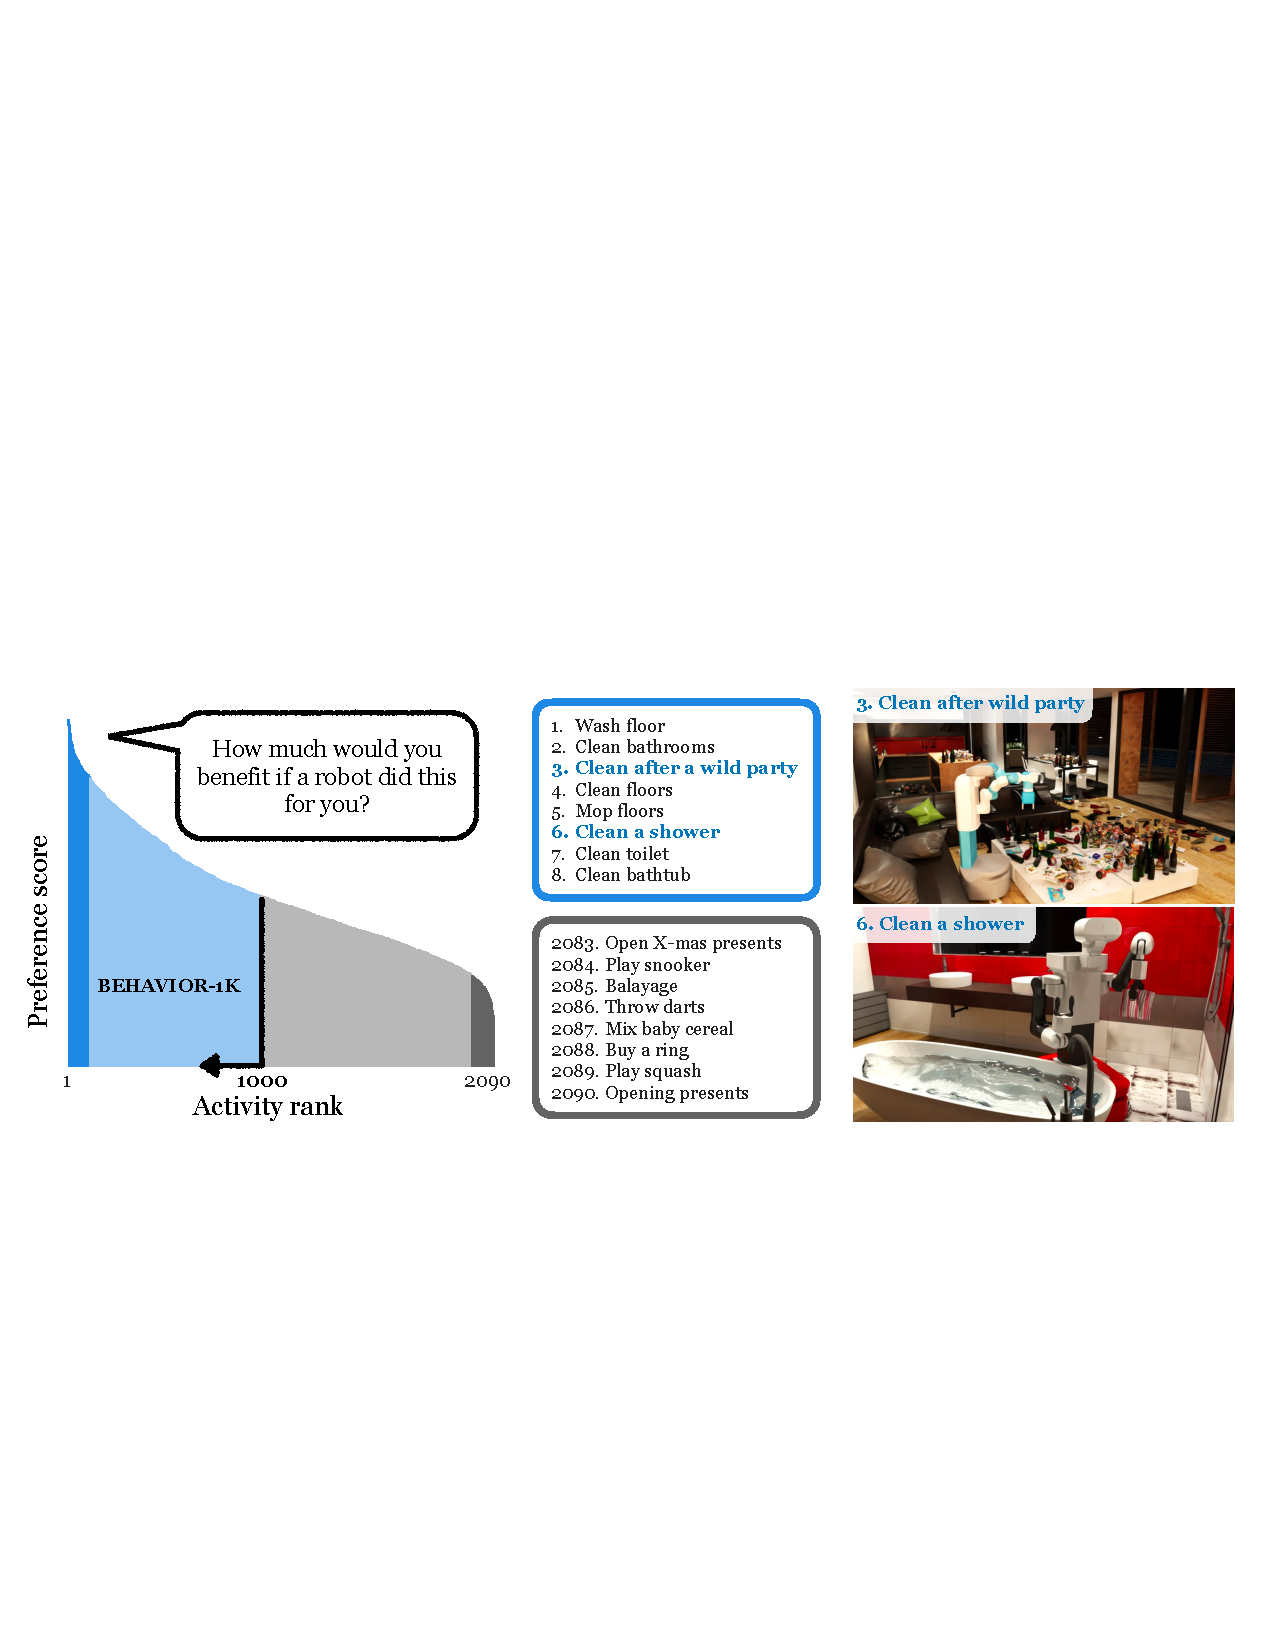
\includegraphics[width=0.99\textwidth]{figures/pull-new.pdf}
\begin{minipage}{0.4\textwidth}
% \includegraphics[width=0.99\textwidth]{figures/survey/all_acts_chart.pdf}
\end{minipage}
%\hfill
% \begin{minipage}{0.58\textwidth}
%  \resizebox{\textwidth}{!}{  
% \begin{tabular}{|c|l|c|l|}
% \hline
% 1 & clean your house after a wild party & 2 & clean a shower \\
% \hline
% 3 & clean grease & 4 & scrubbing bathroom floor \\
% \hline
% 5 & shoveling snow & 6 & washing outside windows \\
% \hline
% 7 & clean walls & 8 & clean up water damage \\
% \hline
% 9 & shovel snow & 10 & clean carpets \\
% \hline
% 11 & clean a grease trap & 12 & emptying trash cans \\
% \hline
% 13 & cleaning pavement & 14 & washing outside walls \\
% \hline
% 15 & washing plates & 16 & sweeping floors \\
% \hline
% 17 & clean the outside of a house & 18 & taking trash outside \\
% \hline
% 19 & clean a couch & 20 & remove hard water spots\\
% \hline
% \end{tabular}
% }
% \end{minipage}
\caption{\textbf{Developing a Human-Centered Benchmark for Embodied AI.} Left: human preference score over 2,090 activities, ranked based on a survey on 1,461 participants. The distribution indicates the high \textbf{diversity} of needs and preferences of humans that should be reflected in a comprehensive benchmark. Middle: Example activities. Laborious activities are ranked the highest, while pleasurable ones are ranked the lowest. Right: visualization of two of the top 8 activities generated by our \textbf{realistic} \simulator simulation environment.}
\label{fig:activity_ranking}
\end{figure}


%%%%%%%% Graveyard of text

%\benchmark is a simulation benchmark for embodied AI and robotics research, which provides realistic simulation of 1000 diverse activities that align with actual human needs. 

% making \simulator one of the most realistic simulators for EAI and robotics research.

% The current AI revolution has been built on top of large benchmarks that provided data and fair conditions to compare solutions~\cite{}. This has been fundamental for the progress in CV~\cite{}, and NLP~\cite{}. However, due to the lack of comprehensive benchmarks, this success has not been yet transferred to some areas of AI. \citet{dehghani2021benchmark} analyzed how the lack of good benchmarking principles for recommendation systems~\cite{} and Atari games~\cite{} is hindering progress and making hard to understand the current state-of-the-art. They call this \emph{rigging the lottery}. In this paper, we present a comprehensive and 



% One of the ultimate goals of these benchmarks is to facilitate the development of smart, effective, robots that facilitate human daily life, i.e., human-centered AIs that ``serve human needs, goals, and values"~\cite{littman2021gathering}. 
% To guide the advances toward this goal, it is critical to have benchmarks that are not only large in scale but that target appropriate tasks, i.e., grounded by actual human needs.
% But, what do humans want robots to do for them? What tasks should we benchmark on?
%\ruohan{realism}To effectively benchmark embodied AI agents in simulation, these benchmarks strive to provide \emph{realistic} simulation that poses similar challenges to those in the real world. %Benchmarks that are not rigorously grounded in actual human needs may pose the risk of driving the community further away from the aforementioned goal.
% What do we benchmark
% Developing a realistic simulator require significant effort, hence we may ask: what tasks should be simulated?


%In our path towards a human-centered benchmark for embodied AI, we need to gain knowledge about the question: \textit{what everyday activities do humans want robots do for them?} We conducted a first-of-its-kind survey with 1,412 participants (details in Sec.~\ref{sec:survey}). The results indicate a clear preference to delegate laborious tasks to robots. However, we also observed that the preferences from humans are extremely \textbf{diverse}, covering a wide range of daily activities. Moreover, we further asked humans to provide definitions of those activities, and this revealed further diversity in type of scenes, objects, physical states, and physical transitions involved. Such diversity is not covered by the existing embodied AI benchmarks. A new, human-centered benchmark needs thus to include a wide range of activities in ecologically diverse settings, pushing robots to overcome the key challenge of learning to generalize.

%Generalization can be more easily developed and tested in simulation. However, towards this goal, an important aspect for a simulation benchmark to enable progress in robotics is to be \textbf{realistic}: it needs to accurately reproduce the characteristics of problems that a robot could encounter in the real-world. While significant advances have been done in benchmarks for specific tasks~\cite{heiden2021disect,urakami2019doorgym,lin2020softgym}, achieving realism for a diverse set of activities is a tremendous challenge due to scientific and engineering effort to provide models, simulation and features. Hence guiding such effort towards realistically simulating a diverse set of activities that are grounded by human needs is important.  

% Generalization is a key goal of AI research, and it is easier to develop and test more general agents in simulation.

% These benchmarks aim to help the development of smart, effective robots that facilitate human daily life -- human-centered AIs that ``serve human needs, goals, and values''~\cite{littman2021gathering, riedl2019human, xu2019toward,shneiderman2020bridging}. Advancing toward this goal requires benchmarks with appropriate tasks, grounded in actual human needs, but this information has been so far missing. %leaving the selection of activities to the criteria of the developers.
\section{Creating a Benchmark Grounded in Human Needs: A Survey Study}
\label{sec:survey}

% Figuring out human needs

% While a significant amount of robotics research aspire to cover human needs, few information can be found about what humans want robots do for them~\cite{}. Since we aim at creating a benchmark that reflects human desires, we cover this lack of information by conducting a survey targeting general U.S. population that asked: \textit{What do you want robots to do for you?} The survey sources 1,990 activities from time-use surveys~\cite{atus,hetus,mtus} and WikiHow articles~\cite{wikihow}. It was conducted on Amazon Mechanical Turk with a total of representative 1412 respondents (see Sec.~\ref{sec:demographics} in our Appendix for demographic information) and 50 responses per activity. 

A significant amount of robotics research aspires to satisfy human needs, but those needs are typically assumed or speculated. Human-centric development requires direct information about what humans want from autonomous agents~\cite{littman2021gathering}. To create a benchmark that reflects these needs, we conduct a survey targeting the general U.S. population that asks: \textit{what do you want robots to do for you?} The survey sources around 2,000 activities from time-use surveys~\cite{atus, hetus, mtus}, which record how people spend their time, and from WikiHow articles~\cite{wikihow}. We conduct the survey on Amazon Mechanical Turk with a total of 1,461 respondents (demographics in Appendix~\ref{sec:demographics}) and fifty 10-point Likert scale responses per activity.

% What are the requirements of a benchmark for that?
Survey results are summarized in Fig.~\ref{fig:activity_ranking} (left), in which we rank the activities based on their human preference score. The full list of ranked activities can be found on our website. The distribution shows large statistical dispersion (Gini index$=0.158$): humans want robots to perform a wide range of activities, from cleaning chores to cooking large feasts. Tedious tasks like ``scrubbing the bathroom floor'' score the highest, while recreational activities like game-play score the lowest. There are around 200 cleaning activities and over 200 cooking activities, among many other categories.

%Yet some mundane but brief tasks like ``turning on the oven'' still score low, likely because of positive but low utility or more potential for interruption than assistance. Ruohan: I don't think this is true: we see turning on the lights
% Activities with extrinsic and intrinsic motivation, like clothes shopping, also score low. Ruohan: not always, let's be careful about the claims

\benchmark activities include the 909 activities with the highest human preference scores and 91 activities from \oldbenchmark~\cite{srivastava2021behavior}, which total the top-ranked 1,000 activities. \benchmark sets itself apart from other embodied AI benchmarks by being sourced from time-use surveys and using survey data to prioritize activities considered most important and useful by humans, and by including a tremendously diverse set of activities. % the resulting activity set creates diversity, another important feature for EAI benchmarks.


% We source from time-use surveys that documentS how humans spend their time~\cite{atus} and selecting according to human preference scores ensure that the final activities reflects actual human need, setting \benchmark apart from other EAI benchmarks. In addition to the realism requirement by simulation benchmarks for EAI, task definitions and simulation in our benchmark should also yield instantiations of the diversity in human needs.  

% \roberto{@sanjana, todo: add figure of the demographics in Appendix: . [In Appendix] (b) Demographic information of the survey participants to show the results are representative} 


% \begin{itemize}
%     \item Two requirements of such a benchmark:
%     \begin{itemize}
%         \item Tasks reflect human preferences for what autonomous agents should do
%         \item Task specification and simulation yields ecologically plausible instantiations of these human preferences 
%     \end{itemize}
%     \item Prior work
%     \begin{itemize}
%         \item Diverse task spaces and fine-grained physical simulation, but short, unrealistic tasks - control benchmarks like SoftGym
%         \item Complex activities, ecologically plausible in some ways, but narrow task space and limited to kinematics, which isn't actually very ecologically plausible
%         \begin{itemize}
%             \item Most direct competitors (VRR, Transport, etc.)
%             \item Cumulative barplot figure
%         \end{itemize}
%     \end{itemize}
%     \begin{itemize}
%         \item Has the underpinnings of a good benchmark, but doesn't target human preference directly (and neither do any of the others)
%         \item BEHAVIOR-100 (but only give it a category of its own in text)
%     \end{itemize}
%     \item Need human preference
%     \begin{itemize}
%         \item Requirement: AI to serve humans, not replace them or grow independently of their needs at all
%         \item Requirement for Embodied AI benchmark: task space that rewards exactly what humans need 
%     \end{itemize}
%     \item How we achieve that 
%     \begin{itemize}
%         \item Survey concept [get quantifiable measure of human preference] % main paper - motivator 
%         \item Considerations [get data from laypeople that is appropriately constrained by the empirical and theoretical limitations of ML decision algos and simulation] % supp
%         \begin{itemize}
%             \item Need layperson respondents 
%             \item Need them to understand what we are asking - ``robot'' is a very overloaded term
%             \begin{itemize}
%                 \item Wording pilot
%             \end{itemize}
%             \item Need *ranking* - we want way to *choose* our 1K activities 
%             \begin{itemize}
%                 \item BWS vs. Likert pilot
%             \end{itemize}
%             \item Limitations of the simulator, and how this can be adapted for other simulators 
%             \begin{itemize}
%                 \item E.g. multiagent, human-agent interaction, more nonkinematic simulated features  
%             \end{itemize}
%         \end{itemize}
%         \item Data source 
%         \begin{itemize}
%             \item *TUS: standard pitch of why they're great 
%             \item WikiHow: If we think it's necessary, we can say that the slightly off-target distribution of WikiHow doesn't matter because we're doing the survey
%         \end{itemize}
%         \item Survey execution details - number of respondents, style of question, etc. [we did quite a big survey indeed] % supp 
%     \end{itemize}
%     \item Survey results 
%     \begin{itemize}
%         \item Overall spread of scores - results have power 
%         \item Sampling of different task results 
%         \begin{itemize}
%             \item Latent variables underlying these preference results 
%             item Categories at each general score level - people want "cleaning" done, they don't always want "shopping" done, they rarely want "playing" done 
%         \end{itemize}
%         \item Demographics
%     \end{itemize}
% \end{itemize}

% Respectful and nuanced way to convince that we're better than others - including B-100
%   - need to say what's new 
% Convince of why the survey is needed, because the adversarial reviewer will ask the so what question, esp since other benchmarks don't have 
% Articulate the difference between them and us - this is a true benchmark, among all the other differences 

% Standalone paper on the social side of survey - esp. with Erik Brynjolfsson 
% Insight companion paper - negative GPT-3 results 
\section{Related Work: Embodied AI Benchmarks}
\label{sec:related}

% salmon color: 

\begin{table}[!t]
    \definecolor{myGrayCell}{rgb}{.8,.8,.8}
    \centering
    \resizebox{\linewidth}{!}{
    \begin{tabular}{|c|c|c|cccccccccccccccccccccc|}
        \rot{} & 
        \rot{} & 
        \rot{\textbf{\benchmark}} & 
        \rot{BEHAVIOR-100} & 
        \rot{AI2THOR Vis. Room Rearr.} & 
        \rot{TDW Transport} & 
        \rot{Rearr. T5 (Habitat)} &
        \rot{ManipulaTHOR ArmPointNav} & 
        \rot{Interactive Gibson Benchmark} & 
        \rot{VirtualHome} & 
        \rot{ALFRED} & 
        \rot{Habitat 2.0 HAB} & 
        \rot{SAPIEN ManiSkill} & 
        \rot{Watch-And-Help} & 
        \rot{RFUniverse} & 
        \rot{Rearr. T2 (OCRTOC)} & 
        \rot{IKEA Furniture Assembly} & 
        \rot{RLBench} & 
        \rot{Metaworld} & 
        \rot{Robosuite} & 
        \rot{SoftGym} & 
        \rot{DeepMind Control Suite} & 
        \rot{OpenAIGym} & 
        \rot{Habitat 1.0} & 
        \rot{Gibson}
        \\\cline{3-25}
        \multicolumn{2}{c}{} & 
        \multicolumn{13}{|c}{Mobile manipulation} & 
        % \multicolumn{2}{|c}{Other planning} & 
        \multicolumn{8}{|c}{Static manipulation} & 
        \multicolumn{2}{|c|}{Navigation}
        \\\cline{2-25}
        
        \rot{} & 
        \multicolumn{1}{|c|}{\begin{tabular}{@{}c@{}}Activities from\\ human preference survey\end{tabular}} &
         \textcolor{indiagreen}\faCheck & 
         \textcolor{red}\faTimes & 
         \textcolor{red}\faTimes & 
         \textcolor{red}\faTimes & 
         \textcolor{red}\faTimes &
         \textcolor{red}\faTimes &
         \textcolor{red}\faTimes & 
         \textcolor{red}\faTimes & 
         \textcolor{red}\faTimes & 
         \textcolor{red}\faTimes & 
         \textcolor{red}\faTimes &  
         \textcolor{red}\faTimes & 
         \textcolor{red}\faTimes & 
         \textcolor{red}\faTimes & 
         \textcolor{red}\faTimes & 
         \textcolor{red}\faTimes & 
         \textcolor{red}\faTimes & 
         \textcolor{red}\faTimes & 
         \textcolor{red}\faTimes & 
         \textcolor{red}\faTimes & 
         \textcolor{red}\faTimes & 
         \textcolor{red}\faTimes & 
         \textcolor{red}\faTimes 
        \\       
        
        \hline
        \rule{0pt}{12pt} & 
         \begin{tabular}{@{}c@{}} Activities\end{tabular} & 
         \textbf{1000} & 
         100 & 
         1 & 
         1 & 
         1 &
         1 & 
         2 & 
         549 & 
         7 & 
         3 &
         4 &
         5 & 
         5 &
         5 & 
         100 & 
         50 & 
         1 & 
         5 & 
         10 & 
         28 & 
         8 & 
         2 & 
         3
        \\

        & 
        \begin{tabular}{@{}c@{}} Scene types \end{tabular} & 
        \textbf{8} & 
        1 & 
        1 &
        1 &
        1 & 
        1 &
        1 &
        1 &
        1 & 
        1 & 
        1 & 
        1 & 
        1 & 
        1 & 
        1 & 
        1 & 
        1 & 
        1 & 
        1 & 
        1 & 
        1 & 
        1 & 
        1
        \\
        % & 
        %  Scenes / rooms &
        % \begin{tabular}{@{}c@{}}\textbf{50 / }\\\textbf{306}\end{tabular} & 
        % \begin{tabular}{@{}c@{}}15 / \\100\end{tabular} & 
        % \begin{tabular}{@{}c@{}}- / \\120\end{tabular} & 
        % \begin{tabular}{@{}c@{}}15 / \\105\end{tabular} & 
        % \begin{tabular}{@{}c@{}}55 static / \\-\end{tabular} & 
        % \begin{tabular}{@{}c@{}}- /\\30\end{tabular} & 
        % \begin{tabular}{@{}c@{}} 10 /\\-\end{tabular} & 
        % \begin{tabular}{@{}c@{}}6 / \\24\end{tabular} &
        % \begin{tabular}{@{}c@{}}- / \\120\end{tabular} & 
        % \begin{tabular}{@{}c@{}}1 / \\6\end{tabular} & 
        % \begin{tabular}{@{}c@{}}1 / \\-\end{tabular} & 
        % \begin{tabular}{@{}c@{}}7 / \\29\end{tabular} & 
        % \begin{tabular}{@{}c@{}}Gibson\end{tabular} &
        % \begin{tabular}{@{}c@{}}1 / \\-\end{tabular} & 
        % \begin{tabular}{@{}c@{}}1 / \\-\end{tabular} & 
        % \begin{tabular}{@{}c@{}}1 / \\-\end{tabular} & 
        % \begin{tabular}{@{}c@{}}1 / \\-\end{tabular} & 
        % \begin{tabular}{@{}c@{}}1 / \\-\end{tabular} & 
        % \begin{tabular}{@{}c@{}}1 / \\-\end{tabular} & 
        % \begin{tabular}{@{}c@{}}1 / \\-\end{tabular} & 
        % \begin{tabular}{@{}c@{}}1 / \\-\end{tabular} & 
        % \begin{tabular}{@{}c@{}}Matterport\\+ Gibson\end{tabular} &
        %  \begin{tabular}{@{}c@{}}572\\static\end{tabular}
        % \\
        & 
         Scenes / rooms &
        \textbf{50/373} & 
        15/100 & 
        -/120 & 
        15/105 & 
        55 static/- & 
        -/30 & 
        10/- & 
        6/24 &
        -/120 & 
        1/6 & 
        1/- & 
        7/29 & 
        Gibson &
        1/- & 
        1/- & 
        1/- & 
        1/- & 
        1/- & 
        1/- & 
        1/- & 
        1/- & 
        HM3D &
        572 static
        \\


        \multirow{1}*{\rotatebox{90}{Diversity}}
         & 
         \begin{tabular}{@{}c@{}} Object categories\end{tabular} & 
         \textbf{1949} & 
         391 & 
         118 & 
         ~50 & 
         YCB & 
         150 & 
         5 & 
         308 & 
         84 & 
         41+YCB &
         4 &
         117 &
         UNK &
         12+YCB & 
         73+ & 
         ~28 & 
         7 & 
         10 & 
         4 & 
         4 & 
         4 & 
         Mtpt. & 
         N/A
        \\
        & 
        \begin{tabular}{@{}c@{}} Object models\end{tabular} & 
        \textbf{9318} & 
        1217 & 
        118 &
        112 & 
        YCB &
        150 & 
        152 & 
        UNK &
        84 &
        92+YCB & 
        162 & 
        UNK & 
        UNK &
        101+YCB & 
        73+ & 
        28 & 
        80 & 
        10 & 
        4 & 
        4 & 
        4 & 
        N/A & 
        N/A
        \\
        % & 
        %  \begin{tabular}{@{}c@{}}\# Object models\\per cat.\end{tabular} & 
        %  \textbf{1-61} & 
        %  1 & 
        %   & 
        %  3 & 
        %  1 & 
        %  12.83 & 
        %  1 & 
        %  1 & 
        %  & 
        %  1 & 
        %  1 & 
        %  1 & 
        %  1 & 
        %  & 
        %  & 
        %  
        % \\
        &
        \begin{tabular}{@{}c@{}} Objs. per activity\end{tabular} & 
        \textbf{3-47} & 
        3-34 & 
        5 &
        7-9 &
        2-5 &
        2-3 & 
        ~10 & 
        1-24 &
        2 &
        5 &
        1 &
        2-8 &
        1-6 &
        5-10 &
        1-2 &
        1-2 &
        1 &
        1-3 &
        1-3 &
        1-3 &
        1 &
        0-1 &
        N/A
        \\        
        
        & 
        \begin{tabular}{@{}c@{}}Diff. state changes \\required per activity \end{tabular} & 
        \textbf{2-11} & 
        2-8 & 
        4 & 
        4 &
        4 &
        2 &
        1-3 & 
        1-7 & 
        2-3 & 
        1-2 &
        1 & 
        1-3 &
        1 &
        1 &
        1-3 & 
        1-4 & 
        4 & 
        1 & 
        1-3 & 
        1-2 & 
        1-2 & 
        1 & 
        1
        \\
        
         & 
        % \begin{tabular}{@{}c@{}}Infinite\\-possible sampling\end{tabular} & 
        \begin{tabular}{@{}c@{}}Infinite scene-\\agnostic instantiation\end{tabular} & 
        \textcolor{indiagreen}\faCheck & 
        \textcolor{indiagreen}\faCheck & 
        \textcolor{red}\faTimes & 
        \textcolor{red}\faTimes & 
        \textcolor{red}\faTimes & 
        \textcolor{red}\faTimes & 
        \textcolor{red}\faTimes & 
        \textcolor{red}\faTimes & 
        \textcolor{indiagreen}\faCheck & 
        \textcolor{indiagreen}\faCheck & 
        \textcolor{red}\faTimes & 
        \textcolor{red}\faTimes & 
        \textcolor{red}\faTimes & 
        \textcolor{red}\faTimes & 
        \textcolor{red}\faTimes & 
        \textcolor{red}\faTimes & 
        \textcolor{red}\faTimes & 
        \textcolor{red}\faTimes & 
        \textcolor{red}\faTimes & 
        \textcolor{red}\faTimes & 
        \textcolor{red}\faTimes & 
        N/A & 
        N/A
        \\ 
        \cline{1-25}

        \rule{0pt}{12pt} 
        & 
        \begin{tabular}{@{}c@{}}Visual quality score\end{tabular} & 
        $\mathbf{3.20}$&
        $1.69$ &
        $1.73$ &
        $1.65$ &
        - &
        $1.73$ &
        - &
        - &
        $1.73$ &
        $1.74$ &
        - &
        - &
        - &
        - &
        - &
        - &
        - &
        - &
        - &
        - &
        - &
        - &
        - 
        \\ 
        & 
        \begin{tabular}{@{}c@{}}Kinematics, dynamics\end{tabular} & 
        \textcolor{indiagreen}\faCheck &
        \textcolor{indiagreen}\faCheck &
        \textcolor{indiagreen}\faCheck &
        \textcolor{indiagreen}\faCheck &
        \textcolor{indiagreen}\faCheck &
        \textcolor{indiagreen}\faCheck &
        \textcolor{indiagreen}\faCheck &
        \textcolor{red}\faTimes &
        \textcolor{indiagreen}\faCheck &
        \textcolor{indiagreen}\faCheck &
        \textcolor{indiagreen}\faCheck &
        \textcolor{red}\faTimes &
        \textcolor{indiagreen}\faCheck &
        \textcolor{indiagreen}\faCheck &
        \textcolor{indiagreen}\faCheck &
        \textcolor{indiagreen}\faCheck &
        \textcolor{indiagreen}\faCheck &
        \textcolor{indiagreen}\faCheck &
        \textcolor{indiagreen}\faCheck &
        \textcolor{indiagreen}\faCheck &
        \textcolor{indiagreen}\faCheck &
        \textcolor{indiagreen}\faCheck &
        \textcolor{indiagreen}\faCheck 
        \\ 
        
        \multirow{1}*{\rotatebox{90}{Realism}} & 
         
        \begin{tabular}{@{}c@{}}Continuous extended\\states (temp., wetness)\end{tabular} & 
        \textcolor{indiagreen}\faCheck & 
        \textcolor{indiagreen}\faCheck & 
        \textcolor{red}\faTimes & 
        \textcolor{red}\faTimes & 
        \textcolor{red}\faTimes & 
        \textcolor{red}\faTimes & 
        \textcolor{red}\faTimes & 
        \textcolor{red}\faTimes & 
        \textcolor{red}\faTimes & 
        \textcolor{red}\faTimes &
        \textcolor{red}\faTimes & 
        \textcolor{red}\faTimes & 
        \textcolor{red}\faTimes & 
        \textcolor{red}\faTimes & 
        \textcolor{red}\faTimes & 
        \textcolor{red}\faTimes & 
        \textcolor{red}\faTimes & 
        \textcolor{red}\faTimes & 
        \textcolor{red}\faTimes & 
        \textcolor{red}\faTimes & 
        \textcolor{red}\faTimes & 
        \textcolor{red}\faTimes & 
        \textcolor{red}\faTimes 
        \\ 
        & 
        \begin{tabular}{@{}c@{}} Flexible materials\end{tabular} & 
        \textcolor{indiagreen}\faCheck & 
        \textcolor{red}\faTimes & 
        \textcolor{red}\faTimes & 
        \textcolor{red}\faTimes & 
        \textcolor{red}\faTimes & 
        \textcolor{red}\faTimes & 
        \textcolor{red}\faTimes &
        \textcolor{red}\faTimes &
        \textcolor{red}\faTimes & 
        \textcolor{red}\faTimes & 
        \textcolor{red}\faTimes & 
        \textcolor{red}\faTimes & 
        \textcolor{indiagreen}\faCheck &
        \textcolor{red}\faTimes & 
        \textcolor{red}\faTimes & 
        \textcolor{red}\faTimes & 
        \textcolor{red}\faTimes & 
        \textcolor{red}\faTimes & 
        \textcolor{indiagreen}\faCheck & 
        \textcolor{red}\faTimes & 
        \textcolor{red}\faTimes & 
        \textcolor{red}\faTimes & 
        \textcolor{red}\faTimes 
        \\ 
        & 
        \begin{tabular}{@{}c@{}}Deformable bodies\end{tabular} & 
        \textcolor{indiagreen}\faCheck & 
        \textcolor{red}\faTimes & 
        \textcolor{red}\faTimes & 
        \textcolor{red}\faTimes & 
        \textcolor{red}\faTimes & 
        \textcolor{red}\faTimes & 
        \textcolor{red}\faTimes &
        \textcolor{red}\faTimes & 
        \textcolor{red}\faTimes & 
        \textcolor{red}\faTimes & 
        \textcolor{red}\faTimes & 
        \textcolor{red}\faTimes & 
        \textcolor{indiagreen}\faCheck &
        \textcolor{red}\faTimes & 
        \textcolor{red}\faTimes & 
        \textcolor{red}\faTimes & 
        \textcolor{red}\faTimes & 
        \textcolor{red}\faTimes & 
        \textcolor{red}\faTimes & 
        \textcolor{red}\faTimes & 
        \textcolor{red}\faTimes & 
        \textcolor{red}\faTimes & 
        \textcolor{red}\faTimes 
        \\ 
        & 
        \begin{tabular}{@{}c@{}}Realistic Fluid\end{tabular} & 
        \textcolor{indiagreen}\faCheck & 
        \textcolor{red}\faTimes & 
        \textcolor{red}\faTimes & 
        \textcolor{red}\faTimes & 
        \textcolor{red}\faTimes & 
        \textcolor{red}\faTimes & 
        \textcolor{red}\faTimes & 
        \textcolor{red}\faTimes & 
        \textcolor{red}\faTimes & 
        \textcolor{red}\faTimes & 
        \textcolor{red}\faTimes &
        \textcolor{red}\faTimes &
        \textcolor{indiagreen}\faCheck &
        \textcolor{red}\faTimes &
        \textcolor{red}\faTimes & 
        \textcolor{red}\faTimes & 
        \textcolor{red}\faTimes & 
        \textcolor{red}\faTimes & 
        \textcolor{indiagreen}\faCheck & 
        \textcolor{red}\faTimes & 
        \textcolor{red}\faTimes & 
        \textcolor{red}\faTimes & 
        \textcolor{red}\faTimes 
        \\ 
        & 
        \begin{tabular}{@{}c@{}}Thermal effects (steam/fire)\end{tabular} & 
        \textcolor{indiagreen}\faCheck & 
        \textcolor{red}\faTimes & 
        \textcolor{red}\faTimes & 
        \textcolor{red}\faTimes & 
        \textcolor{red}\faTimes & 
        \textcolor{red}\faTimes & 
        \textcolor{red}\faTimes & 
        \textcolor{red}\faTimes & 
        \textcolor{red}\faTimes & 
        \textcolor{red}\faTimes & 
        \textcolor{red}\faTimes &
        \textcolor{red}\faTimes &
        \textcolor{indiagreen}\faCheck &
        \textcolor{red}\faTimes &
        \textcolor{red}\faTimes & 
        \textcolor{red}\faTimes & 
        \textcolor{red}\faTimes & 
        \textcolor{red}\faTimes & 
        \textcolor{red}\faTimes & 
        \textcolor{red}\faTimes & 
        \textcolor{red}\faTimes & 
        \textcolor{red}\faTimes & 
        \textcolor{red}\faTimes 
        \\ 
         &
         \begin{tabular}{@{}c@{}}Realistic action execution\end{tabular} & 
         \textcolor{indiagreen}\faCheck &
         \textcolor{indiagreen}\faCheck &
         \textcolor{red}\faTimes &
         \textcolor{indiagreen}\faCheck &
         \textcolor{red}\faTimes &
         \textcolor{indiagreen}\faCheck &
         \textcolor{indiagreen}\faCheck &
         \textcolor{red}\faTimes &
         \textcolor{red}\faTimes &
         \textcolor{indiagreen}\faCheck &
         \textcolor{indiagreen}\faCheck &
         \textcolor{red}\faTimes &
         \textcolor{indiagreen}\faCheck &
         \textcolor{indiagreen}\faCheck &
         \textcolor{indiagreen}\faCheck &
         \textcolor{indiagreen}\faCheck &
         \textcolor{indiagreen}\faCheck &
         \textcolor{indiagreen}\faCheck &
         \textcolor{indiagreen}\faCheck &
         \textcolor{indiagreen}\faCheck &
         \textcolor{indiagreen}\faCheck &
         \textcolor{indiagreen}\faCheck &
         \textcolor{indiagreen}\faCheck 
        \\\cline{1-25}

        % & 
        % \begin{tabular}{@{}c@{}}Realistic\\obs. space\end{tabular} &
        % \textcolor{indiagreen}\faCheck & 
        % \textcolor{indiagreen}\faCheck & 
        % \textcolor{indiagreen}\faCheck &
        % \textcolor{indiagreen}\faCheck &
        % \textcolor{red}\faTimes &
        % \textcolor{indiagreen}\faCheck & 
        % \textcolor{red}\faTimes &
        % \textcolor{red}\faTimes &
        % \textcolor{indiagreen}\faCheck & 
        % \textcolor{indiagreen}\faCheck &
        % \textcolor{indiagreen}\faCheck & 
        % \textcolor{indiagreen}\faCheck & 
        % \textcolor{indiagreen}\faCheck &
        % \textcolor{indiagreen}\faCheck & 
        % \textcolor{indiagreen}\faCheck &
        % \textcolor{indiagreen}\faCheck & 
        % \textcolor{indiagreen}\faCheck &
        % \textcolor{indiagreen}\faCheck 
        % \\
        % & 
        % \begin{tabular}{@{}c@{}}Scenes reconstructed\\from real homes\end{tabular} & 
        % \textcolor{indiagreen} ? &
        % \textcolor{indiagreen}\faCheck &
        % \textcolor{red}\faTimes &
        % \textcolor{red}\faTimes &
        % \textcolor{indiagreen}\faCheck &
        % \textcolor{red}\faTimes &
        % \textcolor{indiagreen}\faCheck &
        % \textcolor{red}\faTimes &
        % \textcolor{red}\faTimes &
        % \textcolor{red}\faTimes &
        % \textcolor{red}\faTimes &
        % \textcolor{red}\faTimes &
        % \textcolor{red}\faTimes &
        % \textcolor{red}\faTimes &
        % \textcolor{red}\faTimes &
        % \textcolor{red}\faTimes &
        % \textcolor{red}\faTimes &
        % \textcolor{indiagreen}\faCheck &
        % \textcolor{indiagreen}\faCheck         

        \rot{} 
        \rule{0pt}{15pt} & 
        \multicolumn{1}{|c|}{\begin{tabular}{@{}c@{}}Benchmark focus: Task-\\Planning and/or Control\end{tabular}} & 
        TP+C & 
        TP+C & 
        TP & 
        TP+C & 
        TP+C & 
        TP+C & 
        C & 
        TP &         
        TP & 
        TP+C & 
        C & 
        TP &
        TP+C &
        TP+C & 
        C & 
        TP+C & 
        C & 
        C & 
        C & 
        C & 
        C & 
        C & 
        C 
        \\\cline{2-25}
    \end{tabular}
  }
  \caption{\textbf{Comparison of Embodied AI Benchmarks:} 
  \benchmark contains 1,000 diverse activities that are grounded by human needs. It achieves a new level of diversity in scenes, objects, and state changes involved. \simulator provides realistic simulation of these 1,000 activities, including some of the most advanced simulation and rendering features such as fluid and deformable bodies. This table is extended from~\cite{srivastava2021behavior}.}

  \label{tab:comparingbenchmarks}
\end{table}



% general role of benchmarks in AI research
% Concrete benchmarks help drive recent advances in AI research by providing an objective lens to track progress, as seen in computer vision~\cite{deng2009imagenet,lin2014microsoft,everingham2010pascal,krishna2017visual,geiger2012we,goyal2017something,sigurdsson2018actor,xiang2017posecnn,martin2021jrdb,caba2015activitynet,gurari2018vizwiz} and NLP~\cite{marcinkiewicz1994building,wang2018glue,rajpurkar2016squad,socher2013recursive,antol2015vqa}. For embodied AI and robotics research, simulation benchmarks~\cite{batra2020rearrangement,weihs2021visual,gan2021threedworld,puig2018virtualhome,shridhar2020alfred,xia2020interactive,yu2020meta,james2019rlbench,savva2019habitat,szot2021habitat} provide lower-cost, faster, and safer training and evaluation. Though simulation provides convenience, real-world robotics challenges await~\cite{kitano1997robocup,wisspeintner2009robocup,iocchi2015robocup,buehler2009darpa,krotkov2017darpa,correll2016analysis,eppner2017lessons,roa2021mobile}, making realism the most common criterion of an embodied AI benchmark's quality. 
 

%????
We provide an extensive comparison between \benchmark, and other embodied AI benchmarks in simulation~\cite{batra2020rearrangement,weihs2021visual,gan2021threedworld,puig2018virtualhome,shridhar2020alfred,xia2020interactive,yu2020meta,james2019rlbench,savva2019habitat,szot2021habitat} in Table~\ref{tab:comparingbenchmarks}. We include a number of factors that contribute to diversity and realism and observe a significant step forward with \benchmark.
First, no other benchmark grounds their activity set on the needs of lay people.  
Other benchmarks often target a relatively restricted set of activities, and their simulators are realistic only in the relevant aspects for those tasks. In fact, we often observe a diversity-realism tradeoff. For instance, instruction-following benchmarks such as VirtualHome~\cite{puig2018virtualhome} and ALFRED~\cite{puig2018virtualhome, shridhar2020alfred} are diverse in the number of scenes, objects, and state changes, but offer a limited low-level physical realism. On the other hand, household rearrangement benchmarks such as Habitat 2.0 HAB~\cite{szot2021habitat}, TDW Transport~\cite{gan2021threedworld}, and SAPIEN ManiSkill~\cite{xiang2020sapien,mu2021maniskill} support realistic action execution and accurate physics simulation for rigid bodies, but only include a handful of tasks. Similarly, SoftGym~\cite{lin2020softgym} and RFUniverse~\cite{fu2022rfuniverse} have the closest simulation features and hence realism to \simulator, but they also lack the task diversity needed to support the development of human-centered general robots. %\benchmark achieves a quantum leap improvement in all crucial dimensions for embodied AI benchmarking.


%B100 motivated by "addressing diversity in human needs"
%We argue that addressing the diversity of human needs is at least as important as realism. 
The most similar benchmark to us is the previous generation \oldbenchmark~\cite{srivastava2021behavior}. \oldbenchmark brought forward several beneficial design choices that we inherit in \benchmark such as the activity sources (ATUS~\cite{atus}), activity definition logic language, and evaluation metrics. However, it fell short in the diversity and realism necessary to support a human-centered embodied AI benchmark in simulation, dimensions where \benchmark achieves unmatched levels.
While \oldbenchmark comprises 100 activities selected by researchers, our \benchmark increases diversity by one order of magnitude, to 1,000 activities, that are grounded in human needs thanks to our unique survey. 
%Table, motivated as comparison in diversity and realism
Furthermore, \oldbenchmark includes only 15 scenes (all houses) and 300+ object categories, while \benchmark increases to 50 scenes (houses, stores, restaurants, offices, etc.) and 1,900+ object categories. In terms of realism, \benchmark extends the simulatable physical states and processes with \simulator: fluids, flexible materials, mixing substances, etc. The realism achieved in rendering by \simulator for \benchmark is also significantly higher than what was possible in \oldbenchmark and other benchmarks (see Fig.~\ref{fig:sim_render}).


% There are a few benchmarks that are built upon the principle of developing human-centered AI, in computer vision~\cite{gurari2018vizwiz}, 



%\input{3-overview}
\section{\dataset}
% \subsection{Obtaining Realistic and Diverse Human-Aligned Activity Definitions}
\label{sec:activity}
% Once activity topics have been sourced to be distributed by human need, they need to be defined concretely. These definitions should reflect intuitive, human instantiations of the activity topics.

\begin{figure}[t]
    \centering
    % IMPORTANT! IF YOU NEED TO MAKE THIS FIGURE SMALLER, ASK CEM TO MAKE HIGHER ASPECT RATIO VERSION SO THAT IT STILL LOOKS FULL-WIDTH
    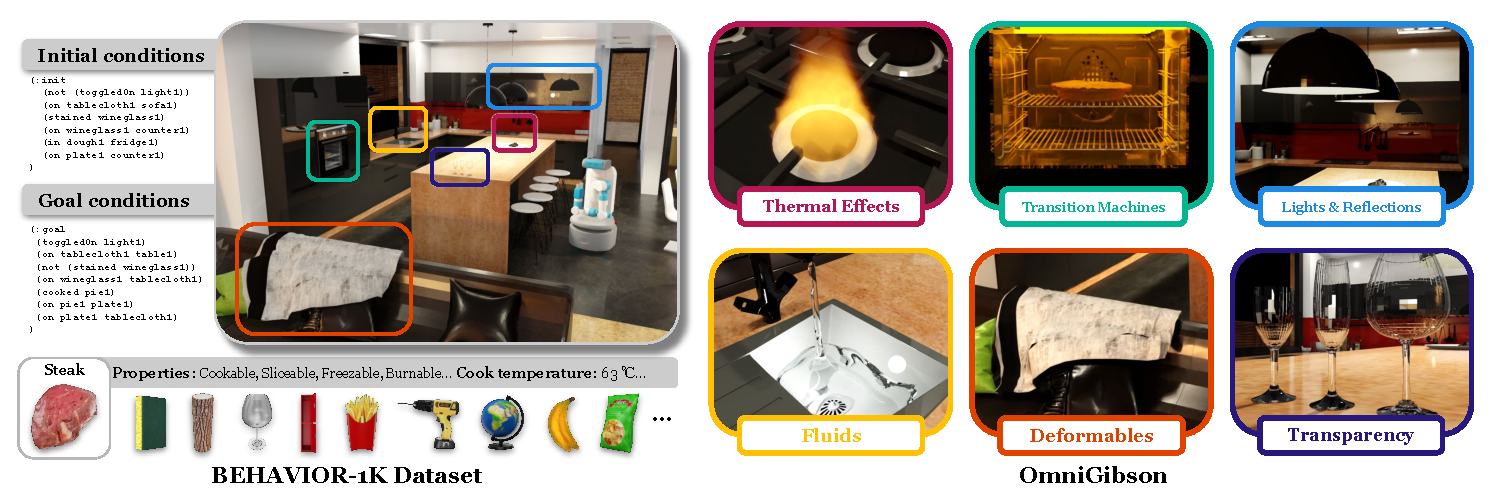
\includegraphics[width=\textwidth]{figures/models/scene_features.pdf}
    \caption{\textbf{Elements of \benchmark.} Our benchmark comprises two elements: \dataset and \simulator. Left: \dataset includes 1,000 BDDL activity definitions (top left), 50 realistic and diverse scenes (top right), and 9,000+ objects with properties annotated in the knowledge base (bottom). Right: \simulator provides the necessary functionalities to realistically simulate the 1000 activities, including thermal effects such as fire/steam/smoke (top left), fluid dynamics (bottom left), functional machines for transition rules (top center), deformable bodies/cloths (bottom center), realistic lighting and reflections (top right), and transparency rendering (bottom right). Together, they constitute a concrete, realistic instantiation of an everyday activity like \texttt{CookingDinner} in simulation.}%A \benchmark scene such as the house scene shown here contains many articulated objects to support this rich set of features.}
    \label{fig:model_vis}
\end{figure}

Once activities have been sourced to reflect human needs, they need to be concretely defined and instantiated the way they would occur in the real world. We build the \dataset, which includes a knowledge base of crowdsourced activity definitions with relevant objects and object states, and a large-scale repository of high-quality, interactive 3D models.

% Sanjana, an important change: we are merging 4.1 and 4.2 and reduce 4.2 to one paragraph. The beginning of 4.1 now will be the beginning of 4. Let me give you some glue starting point - ok
% or you can give it a try. just mention that we creating a database that includes activity defs, knowledge base and models 
% - gave it a pass 

%To get activity definitions that represent human need yet can be simulated and interpreted as reward,
We crowdsource concrete definitions of activities in the form of \bddlfull (\bddl)~\cite{srivastava2021behavior}. \bddl is based on predicate logic and designed to be accessible for laypeople to describe concrete initial and goal conditions for a given activity. Unlike geometric, image/video, or experience goal specifications~\cite{batra2020rearrangement, weihs2021visual}, \bddl definitions are in terms of objects and object states, allowing annotators to define at an intuitive semantic level. The semantic symbols also capture the fact that multiple physical states might be valid initializations and solutions to an activity. See Listings~\ref{lst:bddl3},~\ref{lst:bddl4} and~\ref{lst:bddl5} in Appendix for example definitions.

% To get such representative definitions, \benchmark activities are defined by lay annotators. Crowdsourcing 1,000 ecologically plausible task definitions that can be simulated and interpreted as reward requires a systematic, accessible process. \benchmark definitions are therefore written in \bddlfull (\bddl)~\cite{srivastava2021behavior}. \bddl is based in predicate logic and has custom operators designed for usability, making it a natural way to express concrete initial scenes and general desired goals. Its terms and predicates are objects and states the objects can be in; the annotators are therefore able to write definitions at a semantic level that is more intuitive than arbitrary geometry. The semantic symbols also capture the fact that multiple physical states may be valid initializations and solutions to a task.

The object and object state spaces that activity definitions are built upon are annotated to be ecologically plausible. The object spaces are derived from 5,000 WikiHow articles for the 1,000 activities and mapped to 2,964 leaf-level synsets either from WordNet~\cite{wordnet} or custom-designed. Through crowdworkers, students, and GPT-3~\cite{gpt3}, we also associate each object with our fully simulatable object states: for example, \texttt{apple} is associated with \texttt{cooked} and \texttt{sliced}, but not \texttt{toggledOn}.
%These associations are activity-agnostic, since simulating irrelevant and undesirable states provides important learning signals. 
Many object-property pairs are augmented with parameters, e.g., ``cooked temperature for apples'', taking advantage of \simulator's continuous extended states to make activities especially realistic. Finally, annotators and researchers also create transition rules, e.g., turning tomatoes and salt into sauces, or requiring sandpaper to remove rust. The result is a knowledge base of tens of thousands of elements underlying 1000 ecologically plausible activity definitions. We ensure annotation quality by having five experienced machine learning annotators verify a subset of all types of annotations and receive extremely high approval rates ($>$96.8\%). See Appendix~\ref{as:act_ann} for more details about the knowledge base.

% Along with \bddl to provide intuitive structure, annotators are given ecologically plausible spaces of objects and object states to build definition content from. As seen in Fig.~\ref{fig:activity_pipeline}, we recruit \todo{X} crowdworkers and \todo{Y} students to collect 4,500 WikiHow articles from which we extracted \todo{X} noun phrases and mapped them to 1,484 WordNet~\cite{wordnet} synsets that form \benchmark's object space. With crowdworkers, students, and GPT-3~\cite{gpt3} we also collect annotations for each object with nine unary object states (e.g. ``cooked'', ``toggled on''), four binary states (e.g. ``filled'', ``on top''), and one variable-arity state (``mixed''). Over 20 more states are inferred from these annotations. For eight states and every object they applied to, students also collect parameters (e.g. object-specific ``cook temperature''s). Annotators and researchers finally create realistic cleaning and cooking transitions (such as turning tomatoes and salt into sauce, or using specifically sandpaper to deal with rust instead of a generic cleaning solution) for over 150 activities. 

% We ensure annotation quality by having five experienced machine learning annotators verify 10\% of every crowdsourced or GPT-3-generated pipeline step. All object- and object state-related annotations have >96.8\% approval, and activity definitions have >4.85/5.0 Likert scores for all approval survey questions (see Appendix for details). Furthermore, the goals are verified as logically solvable with \bddl's solver, and the custom annotation software guarantees simulatability in \simulator.

% These rich annotations result in 900 \bddl definitions (examples in fig.~\ref{fig:activity_definition_examples}). To ensure the quality of annotations, we conduct quality assessment by randomly samping 10\% of each annotation generated via crowdsourcing or a learned method, and send them to five experienced machine learning data annotators to verify. The average approval rate is \todo{X} (see Appendix for details).

% Along with \bddl to provide intuitive structure, annotators are given ecologically plausible spaces of objects and object states to build definition content from. Fig.~\ref{fig:activity_pipeline} outlines each step of this data collection: overall, we collect 4,500 WikiHow articles, extract \todo{XX} noun phrases from them, and finalize 1,484 object terms that span the object spaces of each activity. Each object term is mapped to a WordNet~\ref{wordnet} synset, eliminating ambiguity and providing taxonomic structure. We associate each of these objects with over 35 fully simulated object states, thereby collecting over 50,000 annotations from humans and GPT-3~\cite{gpt3}

% Activity definition results (referring to Table 1)
% With this pipeline, we recruited X humans (X upworkers, Y students) work on ...
% 4500 articles, X noun phrases, X objects, X object states (X unary Y binary Z unary, can use a few examples), X types of transition maps (including recipes),  X object state parameters, which lead to 900 BDDL definitions. Example BDDL definitions can be seen in Fig.~\ref{fig:activity_definition_examples}. To ensure the quality of annotations, we conduct quality assessment by randomly sample x\% of annotations, and send them to X to verify. The average approval rate is X (see Appendix for details). 

The diversity of these activity definitions requires diverse object and scene models. % and (b) realistic simulation of different physical states and processes (see Sec.~\ref{sec:simulation}). 
On top of the 15 house scenes from \oldbenchmark~\cite{srivastava2021behavior}, we acquire 35 fully interactive scenes across diverse scene types, such as gardens, offices, restaurants, and stores, that are essential for everyday activities. This is unprecedented compared to other benchmarks (see Table~\ref{tab:comparingbenchmarks}). We also acquire 9,000+ object instances across 1,900+ categories required by the activities, and annotate rich physical (e.g., friction, mass, articulation) and semantic properties (e.g., category) for each object. Representative scene and object models can be seen in Fig.~\ref{fig:model_vis}. More details of the 3D models can be found in Appendix~\ref{as:modeling}.

% bddl1: simple, involves substances and complex cleaning 
% bddl2: moderate, involves assembly? 
% bddl3: most complex, involves comp/decomp
% bddl4: b100 - some pick and place that involves basic cleaning 
% bddl5: b100 - some long pick and place
% \todo{cite gpt3}



% \item All previous common sense knowledgebase are insufficient due to B1K's diversity (Table \ref{tab:activity_cskb}), so we create B1K dataset to support B1K activity definition. 

% - good benchmarking and simulation requires parametrization with data that is 
%     - ecologically plausible 
%     - grounded in human preference
% - Prior work?
%       - at least involve it so i can cite all the other benchmarks 
% - Definitions - two parts, the underlying data and the symbolic language for specification
% - Annotations to get data for definitions
%     - Realistic 
%     - Grounded 
%     - Human preference
% - Symbolic language
%     - Human preference: semantic, custom quantifiers 
%     - Eco plaus: all kinds of new features
%           - cite prior attempts 
%     - BDDL repo
% - Definition annotations
%     - Interface
% - Quality metrics
% - BEHAVIOR symbolics create appropriate challenge
% - Impact



% Once activity topics have been sourced to be distributed by human need, they need to be defined concretely. These definitions should reflect intuitive, human instantiations of the activity topics, and have the richness seen for the same task in the real world. 

% To get such representative definitions, \benchmark activities are defined by lay annotators. Collecting ecologically plausible task definitions that can be simulated is a major design problem. Collecting 1,000 requires a systematic process, and crowdsourcing requires it to be accessible. We therefore use \bddlfull (\bddl)~\cite{srivastava2021behavior} and offer annotators a visual versoin~\cite{srivastava2021behavior}. \bddl is predicate logic-based and inspired by PDDL~\cite{mcdermott1998pddl}, with custom operators to make it more accessible. As a formalization of human reasoning, it is a natural way to describe an environment and express desired goals. In \bddl, logic constants and variables are objects and predicates are states of the objects, meaning the definitions are built at a semantic level. The semantic symbols are intuitive for laypeople, and they capture the fact that there are multiple reasonable simulator configurations that both instantiate and solve these complex and naturalistic tasks.
% \todo{correctly reference supplementary bddl}

% To ensure that not only the structure but the content of the definitions are as reflective of human need as possible, we equip annotators with ecologically plausible object spaces and realistic object-state associations. Each activity's object space is sourced from from five relevant WikiHow~\cite{wikihow} articles, since WikiHow is a prevalent and crowdsourced database of items needed to do a task. Each object is mapped to a WordNet~\cite{wordnet} synset to avoid word sense ambiguity and obtain taxonomic structure in the object space. These objects are then associated with each of our 35+ fully simulated object states\textemdash for example, ``apple'' is associated with ``cooked'' and ``frozen'' but not ``toggled on''. Associations are determined activity-agnostically because it should always be possible to enter irrelevant and undesired object states, as common sense and safety signals are important to learning human need. Object-state associations are also annotations, collected from foundation models (FMs)~\cite{bommasani2021opportunities}, specifically GPT-3~\cite{gpt3}, or humans where necessary. This set of sources makes the definition substrates ecologically plausible and scalable to collect. 

% The combination of intuitive, semantic \bddl structure and ecologically plausible content spaces make it possible for us to collect naturalistic definitions that are free from researcher bias at scale. Lsts.~\ref{lst:bddl1},~\ref{lst:bddl2}, and~\ref{lst:bddl3} show \benchmark definitions of increasing difficulty. Compared to \bddl definitions from \oldbenchmark (lsts.~\ref{lst:bddl4} and~\ref{lst:bddl5}, the activity length is of similar range but the expressiveness is much higher - in \benchmark, arbitrarily subdividable substances like flour or juice can be represented generally as objects and cleaning is more substance-specific than simply cleaning implement and water, and we can transform sets of objects into new objects as in building or cooking.









% \subsection{Creating Diverse 3D Scene and Object Models}
% \label{sec:model}

% On top of the 15 house scenes from \oldbenchmark~\cite{srivastava2021behavior}, we acquired 35 new, fully interactive scenes across diverse scene types such as gardens, offices, restaurants, grocery stores, that are essential for everyday human activities, which is unprecedented compared to other EAI benchmarks (see Table~\ref{tab:comparingbenchmarks}). We also acquired 3,300+ object instaces across 1,200 categories needed for the activities and annotated rich physical (friction, mass, articulation, etc), and semantic properties (category, heat/light/water source location, etc) for each object. Representative scene and object models can be seen in Fig.~\ref{fig:model_vis}, and additional information can be found in Appendix.

% The 1000 activities selected and defined by humans require a diverse set of object and scene models to be performed in simulation. These models have to be as realistic as possible (visually, physically) to aim the development of embodied AI solutions.
% We acquire scenes and object 3D models from 3D artists covering a diverse set of scene types that are essential for everyday human activities, including apartments, houses, gardens, grocery stores, generic halls, hotels, offices, restaurants, schools, public restrooms, and commercial kitchens (Table~\ref{tab:comparingbenchmarks}).
% These scenes are fully interactive: we annotate missing articulation and any other physical property. 

% \roberto{in Appendix: all \dataset object models in Fig.~\ref{fig:model_object}.  Fig.~\ref{fig:model_scene}. Table~\ref{tab:model_scene} provides details of each scene.
% }

% the activity definitions, it is evident that these 1000 diverse activities require a large number of interactive, high quality 3D models for daily scenes and objects. 

% For scene models, we used 15 scenes from \oldbenchmark, and purchased 35 scenes from 3D artists online, covering a diverse set of scene types that are essential for everyday human activities, including apartments, houses, gardens, grocery stores, generic halls, hotels, offices, restaurants, schools, public restrooms, and commercial kitchens (Table~\ref{tab:comparingbenchmarks}). Many of the scenes are large-scale: the number of object types can be as many as 137 (e.g. in a large house scene), and the number of instances as many as 6994 (e.g. in a grocery store scene). For these scenes to be useful for EAI research, they need to be fully \emph{interactive}. We manually process these scenes by segmenting all rooms, walls, floors, and objects properly. Scene modeling results can be visualized in Fig.~\ref{fig:model_vis}, Fig.~\ref{fig:model_scene}. Table~\ref{tab:model_scene} provides details of each scene.  

% %iG: 30/100+, need to check numbers. 
% For object models, we purchased X object models online. Many of our object models include common daily objects (e.g., IKEA furnitures, daily objects) that can be acquired and used for sim2real experiments (Sec.~\ref{sec:sim2real}). Again, to create full interactive scenes, we manually process these models by: (a) annotating object local coordinate frames; (b) performing moderate vertex reduction to ensure rendering speed while maintaining visual quality; (c) matching the object categories to WordNet synsets in activity definitions. In addition, we conduct additional post-processing for (a) articulated objects: annotating the joint configurations (e.g. joint type, origin, axis, limits); (b) light objects: annotating the light source type, location and intensity; (c) objects with certain states: annotating locations of heat source, water source, toggle button, and so on. %(c) annotating deformable objects \ruohan{@Eric} by ...; (c) annotating whether an object is consisted of particles \ruohan{@Eric}.  
 









\section{\simulator: Instantiating \benchmark with Realistic Simulation}
\label{sec:simulation}

\begin{figure}[t]
\captionsetup[subfloat]{labelformat=empty}
\captionsetup[subfloat]{justification=centering}
\centering
\subfloat[][\textbf{\simulator\\ $\mathbf{3.20\pm1.23}$}]{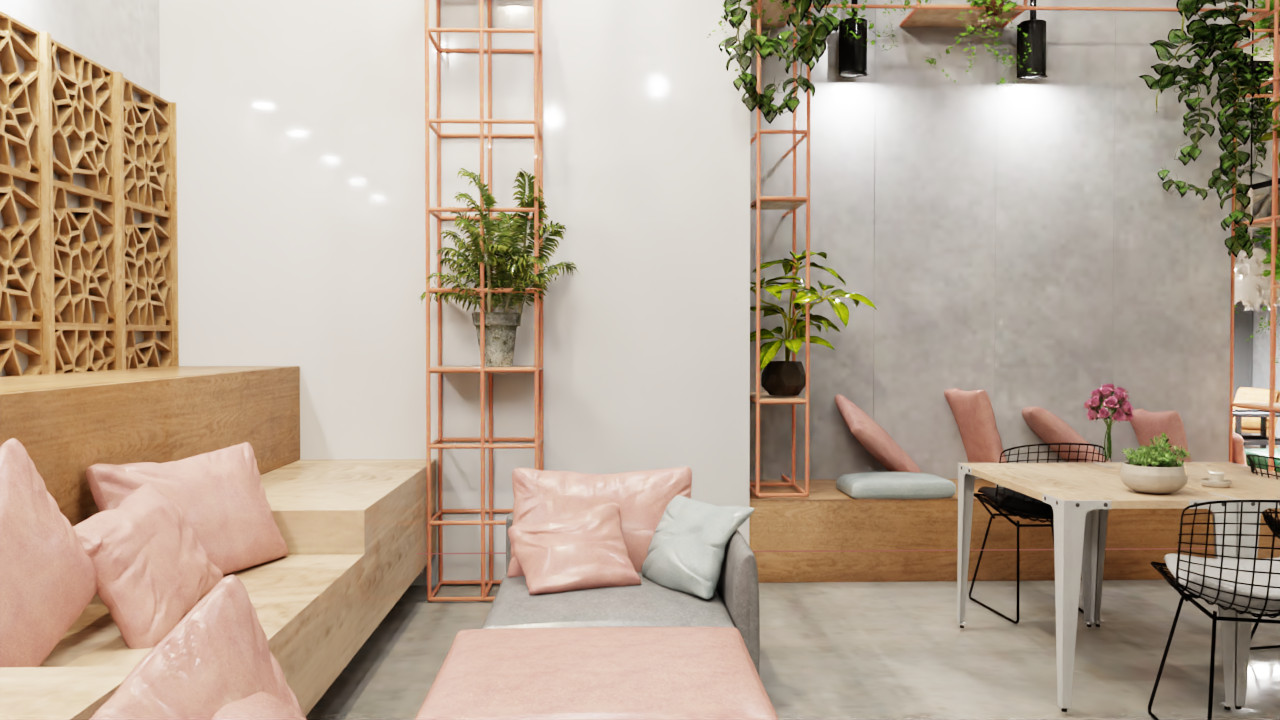
\includegraphics[width=.199\textwidth]{figures/omnigibson/og_sample.jpg}}
\hfill
\subfloat[][Habitat 2.0\\ $1.74\pm1.33$]{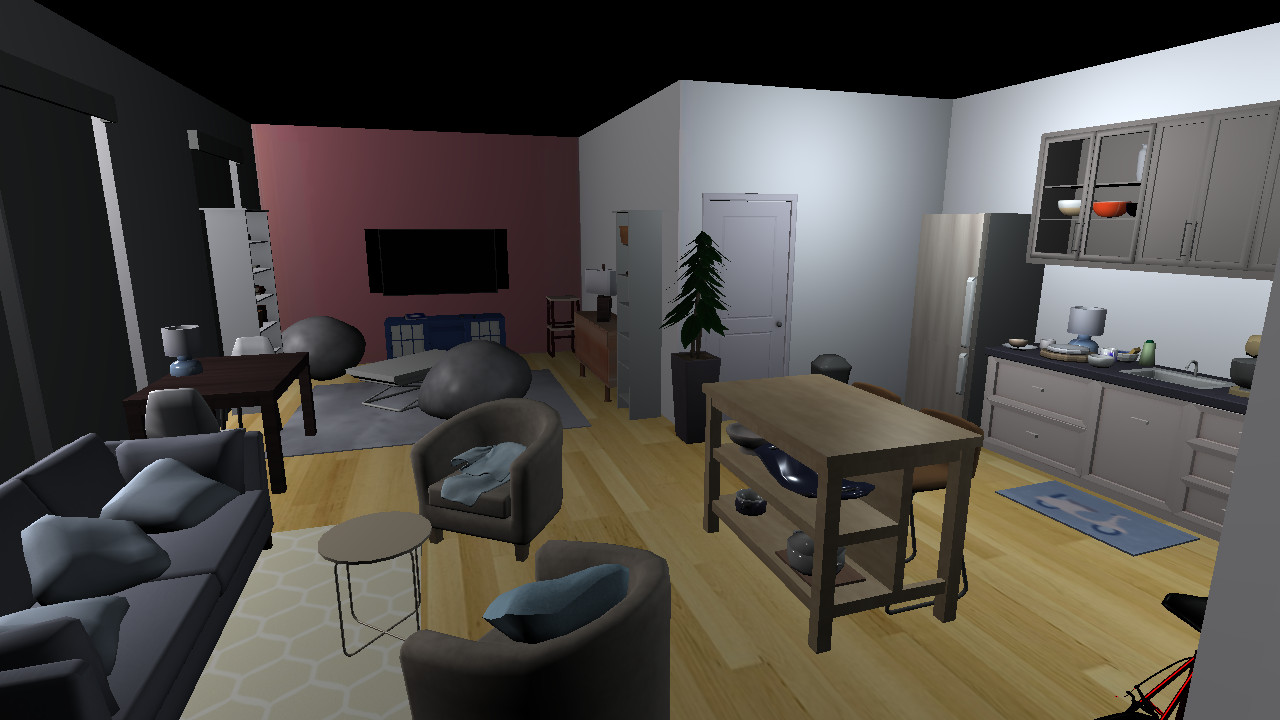
\includegraphics[width=.199\textwidth]{figures/omnigibson/habitat_sample.jpg}}
\hfill
\subfloat[][AI2-THOR\\ $1.73\pm1.37$]{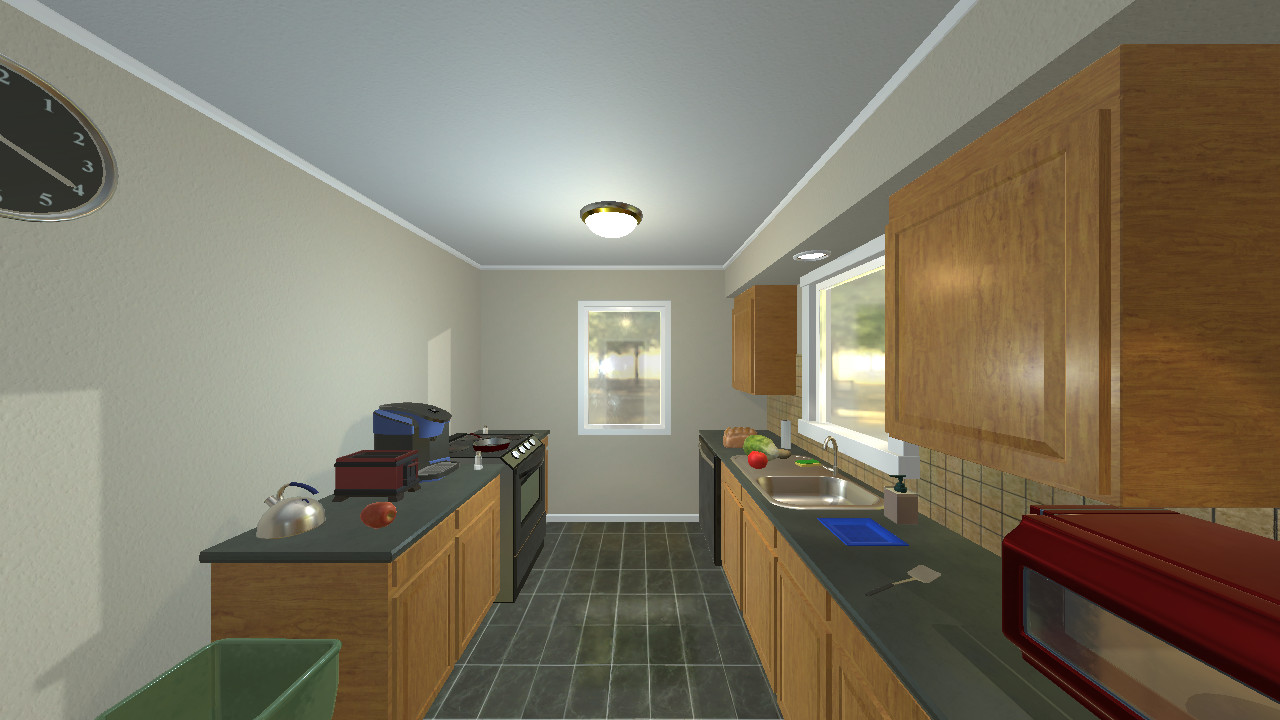
\includegraphics[width=.199\textwidth]{figures/omnigibson/ai2_sample.jpg}}
\hfill
\subfloat[][iGibson 2.0\\ $1.69\pm1.24$]{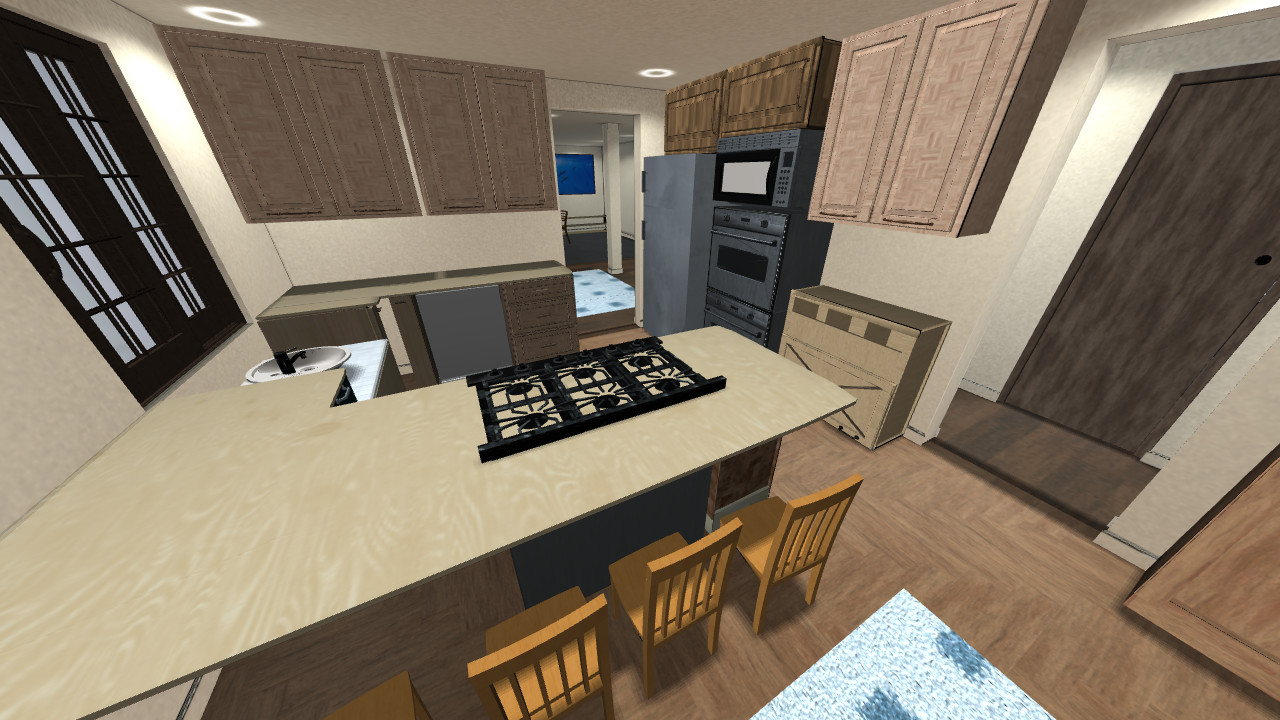
\includegraphics[width=.199\textwidth]{figures/omnigibson/ig2_sample.jpg}}
\hfill
\subfloat[][ThreeDWorld\\ $1.65\pm1.23$]{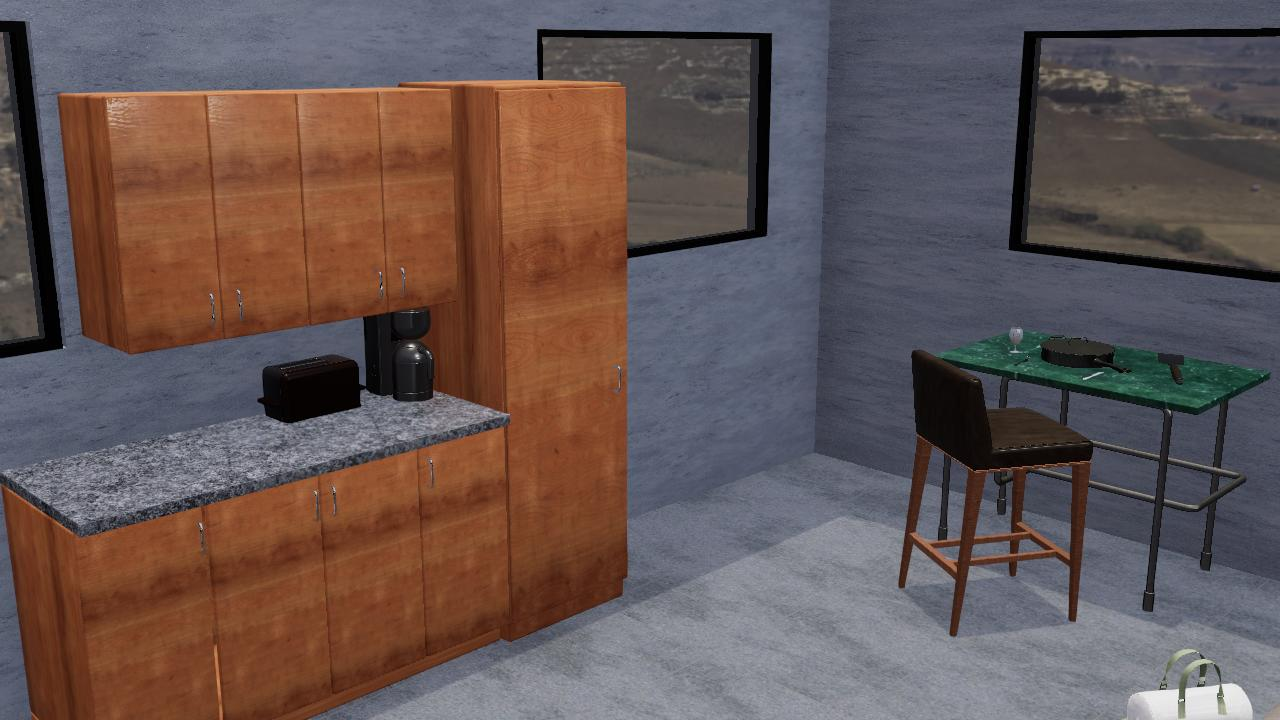
\includegraphics[width=.199\textwidth]{figures/omnigibson/tdw_sample.jpg}}
% \begin{subfigure}{.19\textwidth}
% 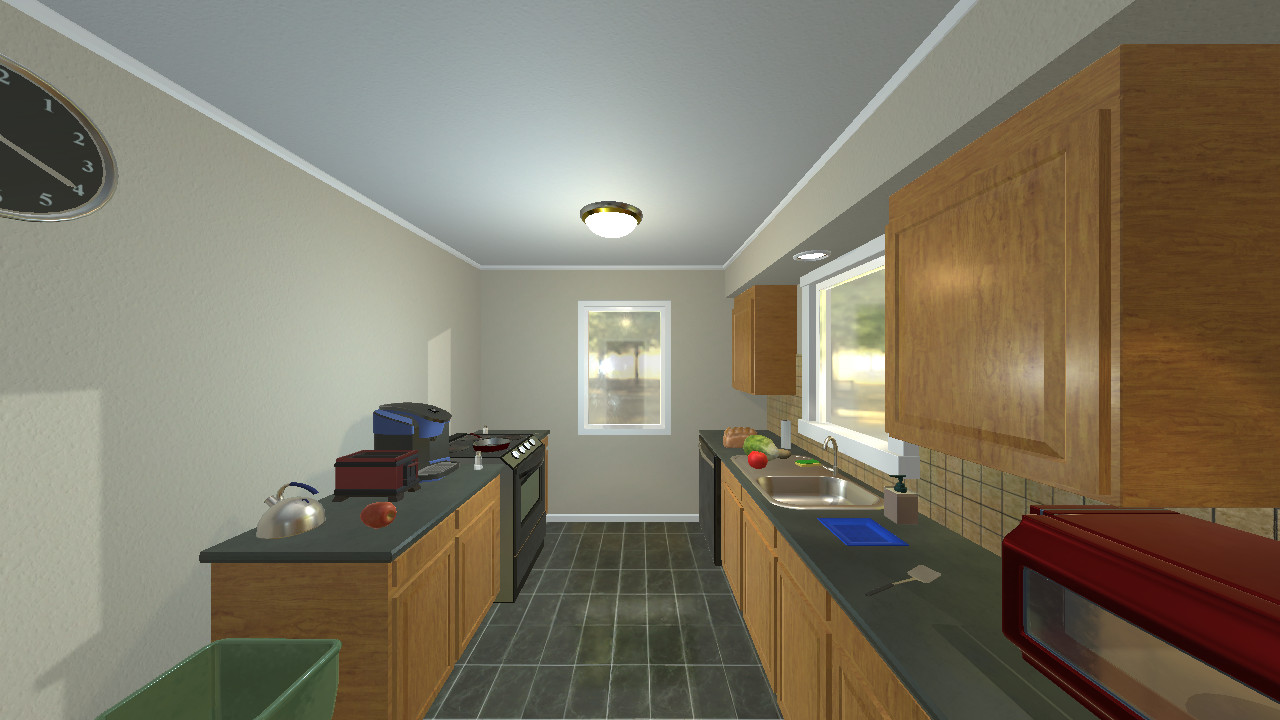
\includegraphics[width=\textwidth]{figures/omnigibson/ai2_sample.png}
% \caption{AI2Thor: $3.27\pm1.25$}
% \end{subfigure}
% \begin{subfigure}{.19\textwidth}
% 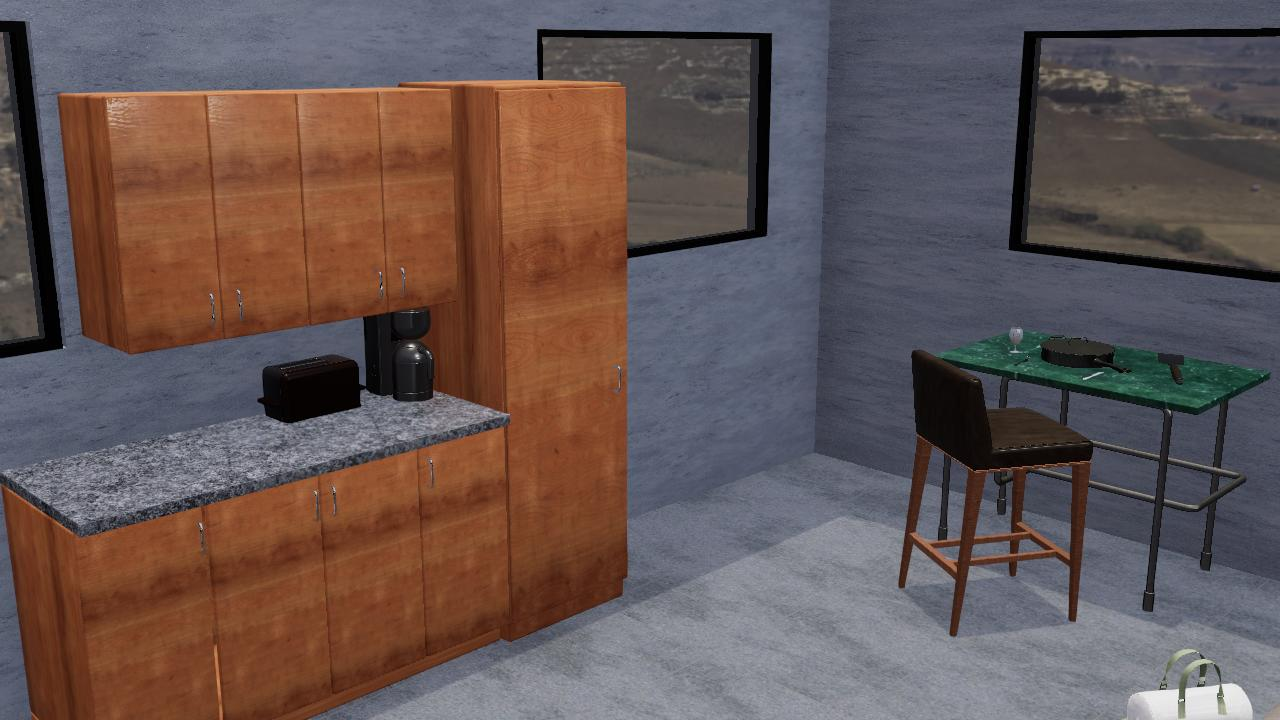
\includegraphics[width=\textwidth]{figures/omnigibson/tdw_sample.jpg}
% \caption{ThreeDWorld: $3.37\pm1.23$}
% \end{subfigure}
% \begin{subfigure}{.19\textwidth}
% 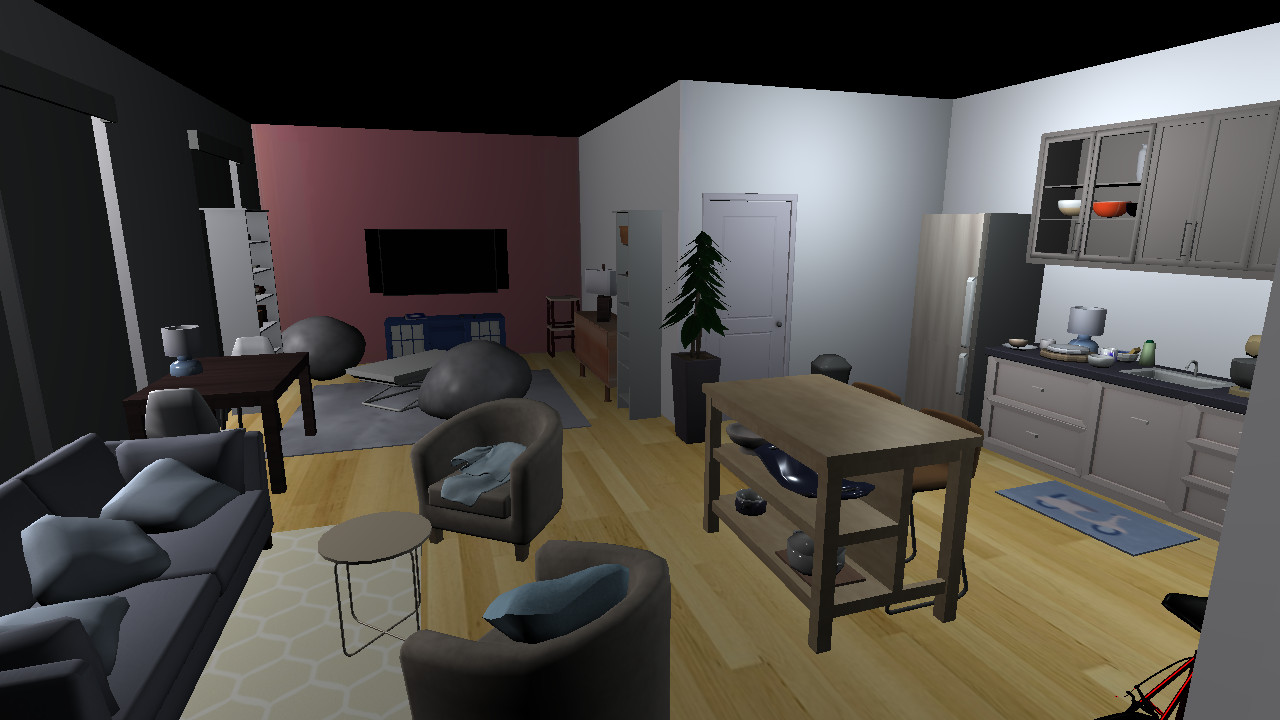
\includegraphics[width=\textwidth]{figures/omnigibson/habitat_sample.png}
% \caption{Habitat2.0: $3.27\pm1.32$}
% \end{subfigure}
% \begin{subfigure}{.19\textwidth}
% 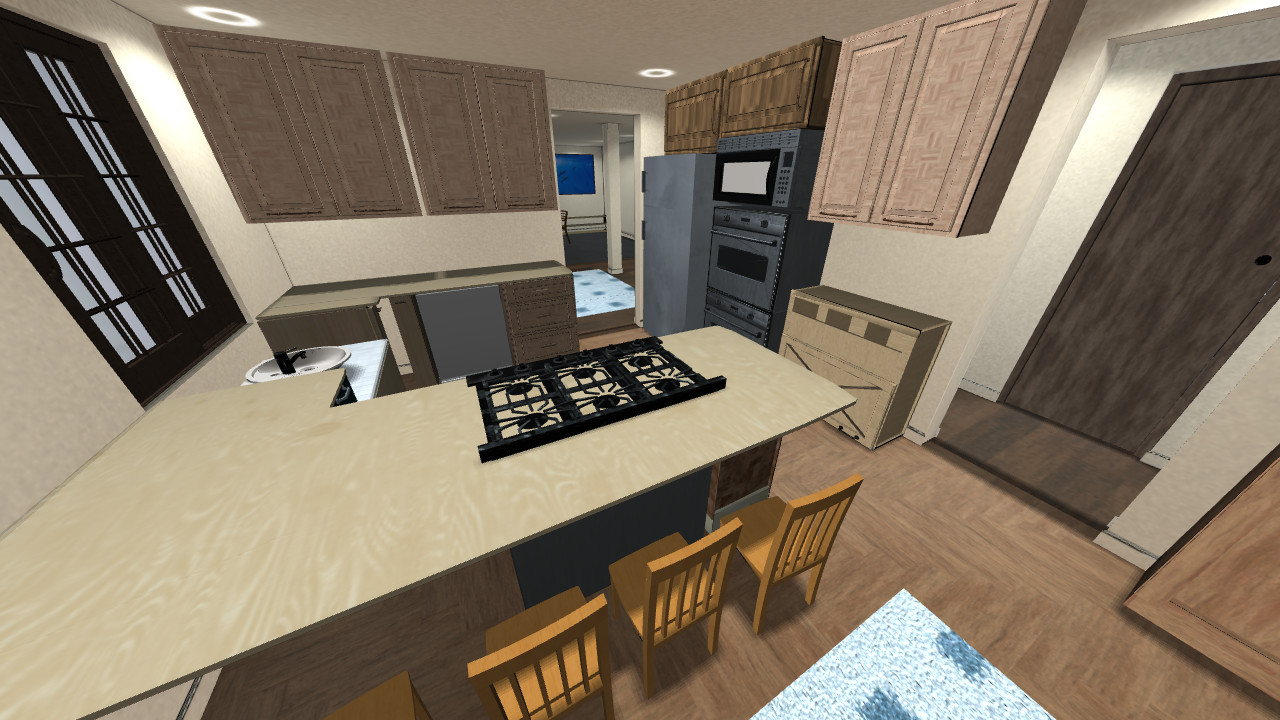
\includegraphics[width=\textwidth]{figures/omnigibson/ig2_sample.png}
% \caption{iGibson2.0: $3.27\pm1.25$}
% \end{subfigure}
\vspace{15pt}
\caption{\textbf{Comparison of Visual Realism:} We evaluate \simulator's visual realism against other simulation environments by running a survey with 60 human subjects. We ask them to rank the realism of sampled images from each environment with a score of 5 (most realistic) to 1 (least realistic). We report the mean and standard deviation and show a sampled image from the study. We observe that the participants consider \simulator to be significantly more visually realistic than all other environments. See Appendix~\ref{amt_study_appx} for more info.}
\label{fig:sim_render}
\end{figure}

% diversity + realism
%An important characteristic of \oldbenchmark is that it's not bounded to any specific simulation environment~\cite{behinh2}, although a fully functional implementation in iGibson 2.0~\cite{li2021ig2} is provided.
%As we use the same general logic language (BDDL) to define activities, we are able to maintain this benefit in \benchmark.
\oldbenchmark is implemented in iGibson 2.0~\cite{li2021ig2}; however, realistic simulation of the diverse activities in \benchmark is beyond the capability of iGibson 2.0. We present a novel simulation environment, \simulator, that provides the necessary functionalities to support and instantiate \benchmark.
\simulator is built on top of Nvidia Omniverse and PhysX 5, providing the simulation of not only rigid bodies, but also deformable objects, fluids, and flexible materials (see Fig.~\ref{fig:sim_obj_prop}), while generating highly realistic ray-traced or path-traced virtual images (see Fig.~\ref{fig:sim_render}).
These features significantly boost the realism of \benchmark compared to other benchmarks.


Similar to \oldbenchmark, \simulator also simulates additional, non-kinematic extended object states (e.g., temperature, soaked level) based on heuristics (e.g., temperature increases when being next to a heat source that is toggled on). \simulator also implements the functionalities to generate infinite valid physical configurations that satisfy the activities' initial conditions as logical predicates (e.g. \texttt{food} is \texttt{frozen}), and to evaluate their goal conditions (e.g. \texttt{food} is \texttt{cooked} and \texttt{onTop} of a \texttt{plate}, the \texttt{cloth} is \texttt{folded}) based on the object's physical states (pose and joint configuration) and extended states. \revision{\simulator natively supports randomization during scene initialization and can sample amongst object models and their poses/states.} The full details of extended object states and logical predicates that \simulator supports can be found in Appendix~\ref{as:object_states}. 

% However, the current simulators' features are insufficient to fully capture many of \benchmark's key properties, such as fluids, deformables, and high-fidelity rendering. 
% To that end, we present \simulator, a state-of-the-art simulator built upon NVIDIA's Omniverse physics and rendering engine and iGibson's~\cite{li2021ig2} infrastructure that enables \benchmark to be fully realized in simulation. \simulator provides 3 key properties crucial to instantiating \benchmark: (1) Accurate simulation of \textbf{complex physical processes} (Fig.~\ref{fig:sim_obj_prop}), (2) \textbf{visual realism} via high-fidelity, super real-time raytraced rendering (Fig.~\ref{fig:sim_render}), and (3) grounded \textbf{perceptual modules} to drive multi-modal embodied AI research (Fig.~\ref{fig:sim_modalities}). \eric{Do we want to highlight (3) this much? This seems to be a basic requirement of any simulator.}

%\subsection{Simulating Complex Physical Processes}

Many everyday tasks are difficult to simulate because they require modeling complex physical processes, such as folding a towel or pouring a glass of water. \simulator unlocks them by supporting realistic simulation of fluids, deformable bodies, and cloths (see Fig.~\ref{fig:model_vis}). Indeed, without these features, over half of \benchmark activities would not be simulatable, highlighting how crucial these features are for capturing everyday activities. \simulator also captures multiple physical processes that are not natively simulatable by Omniverse, such as baking pies or pureeing vegetables. Aside from the extended states mentioned above, we also design a modular \textit{Transition Machine}, which specifies custom transitions between groups of objects when specified conditions are met. For example, a dough placed inside an oven that reaches a certain temperature threshold will turn into a pie. This further expands \simulator's capacity to simulate complex, realistic activities that would otherwise be intractable to fully simulate physically.

% \subsection{High-Fidelity Rendering for Visual Realism}

% Visual realism has been a key limiting factor of current simulation platforms. While rendering capabilities in other simulators have improved significantly during recent years, the sim2real visual domain gap remains quite evident. \simulator substantially improves current state-of-the-art simulation rendering by providing super real-time raytracing, enabling high-fidelity visuals that include realistic visualization of fluids, transparencies, and lights. Moreover, for even greater visual fidelity, \simulator can also leverage path-tracing to render hyper-realistic images. These features considerably reduce the visual domain gap between simulation and reality, and we measure the relative improvement quantitatively by evaluating \simulator's visual quality against current state-of-the-art embodied AI simulators (Fig.~\ref{fig:sim_render}). \eric{And we will get favorable ratings from MTurks?}

% \subsection{Grounding Agent Interactions via Perceptual Modules}

% \eric{In this section, maybe we can claim we provide realistic agent sensing AND actuation, not just sensing alone}
% \fei{suggest changing subsection title to realistic sensing and actuation}

% \fei{This subsection needs to be grounded in numbers or qualitative results, maybe a figure like relmogen paper figure A.5}
% \simulator is agent-centric, and emphasizes grounded interactions between embodied agents and their environment. To that end, \simulator provides diverse perceptual modules to capture realistic sensor modalities from an agent's perspective, including RGB, Depth, Semantic Segmentation, Normal, and Optical Flow images, in addition to non-visual modalities such as proprioception and Lidar scans (Fig.~\ref{fig:sim_modalities}). \simulator also provides varying abstraction levels for agent action spaces, including low-level control, assistive manipulation, and primitive skill execution. Overall, these modules are intended to be useful to the broad embodied AI research community, with the goal of accelerating breakthroughs on \benchmark.


% \eric{In B100 and iG 2.0, we focus a lot on talking about object-centric physical properties (kinematic and non-kinematic) and unary/binary predicate checking/sampling/update mechanism). Do we want to re-iterate these (with the new states added, of course)?} 


% \simulator increases realism in both precision in physics and quality in visuals,

% \begin{enumerate}
%     \item The diversity of these 1K activities require simulating complex physical phenomena (Fig.~\ref{fig:sim_obj_prop}). Built upon Nvidia's Omniverse and iGibson~\cite{li2021ig2}, OmniGibson supports new features, including particles, deformables, transparency, and mixtures of materials (Fig.~\ref{fig:sim_physics}).
%     \item OmniGibson has extremely high rendering quality, with an option to enable super high quality rendering through path tracing technique (Fig.~\ref{fig:sim_render}). 
%     \item OmniGibson's perceptual module will provide utilities for embodied AI research, such as different visual modalities, including RGB images, depth, semantic / instance segmentation, optical flow, scene graph, etc (Fig.~\ref{fig:sim_modalities}).  
%     \item Rendering speed test results and comparison with other benchmarks. Ideally, we can show that OmniGibson achieves high-quality rendering without sacrificing rendering speed, but this is unknown at this point.  
%     \item Although OmniGibson is the only simulator that can support B1K now, in the future, B1K is simulator agnostic and can be implemented in any simulator that is as powerful as OmniGibson. 
% \end{enumerate}


% \begin{figure}[h]
%     \centering
%     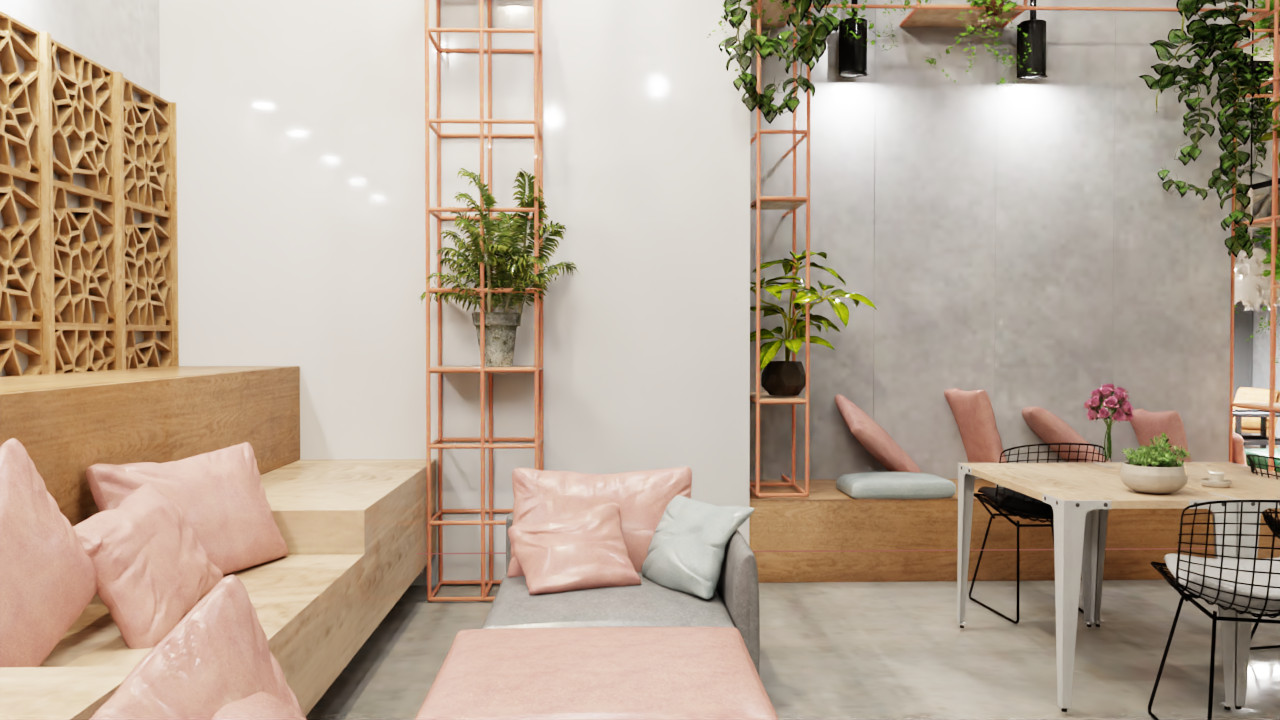
\includegraphics[width=0.19\textwidth]{figures/omnigibson/og_sample.png}
%     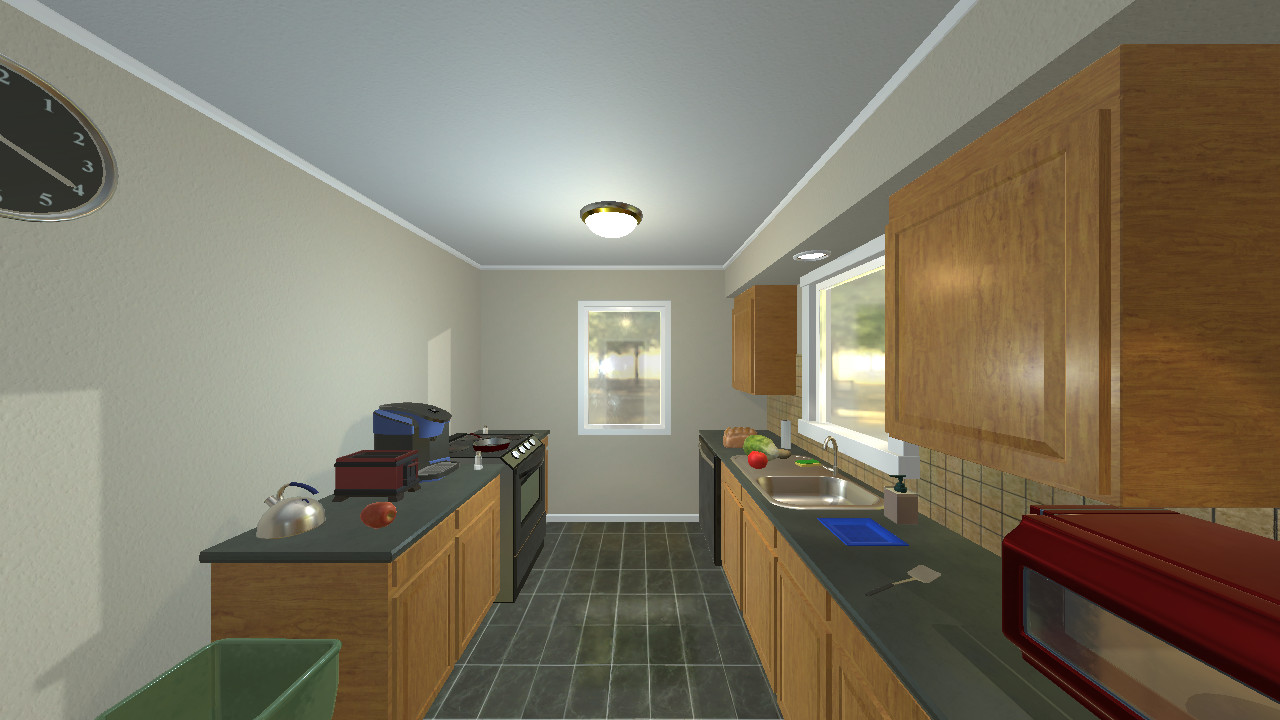
\includegraphics[width=0.19\textwidth]{figures/omnigibson/ai2_sample.png}
%     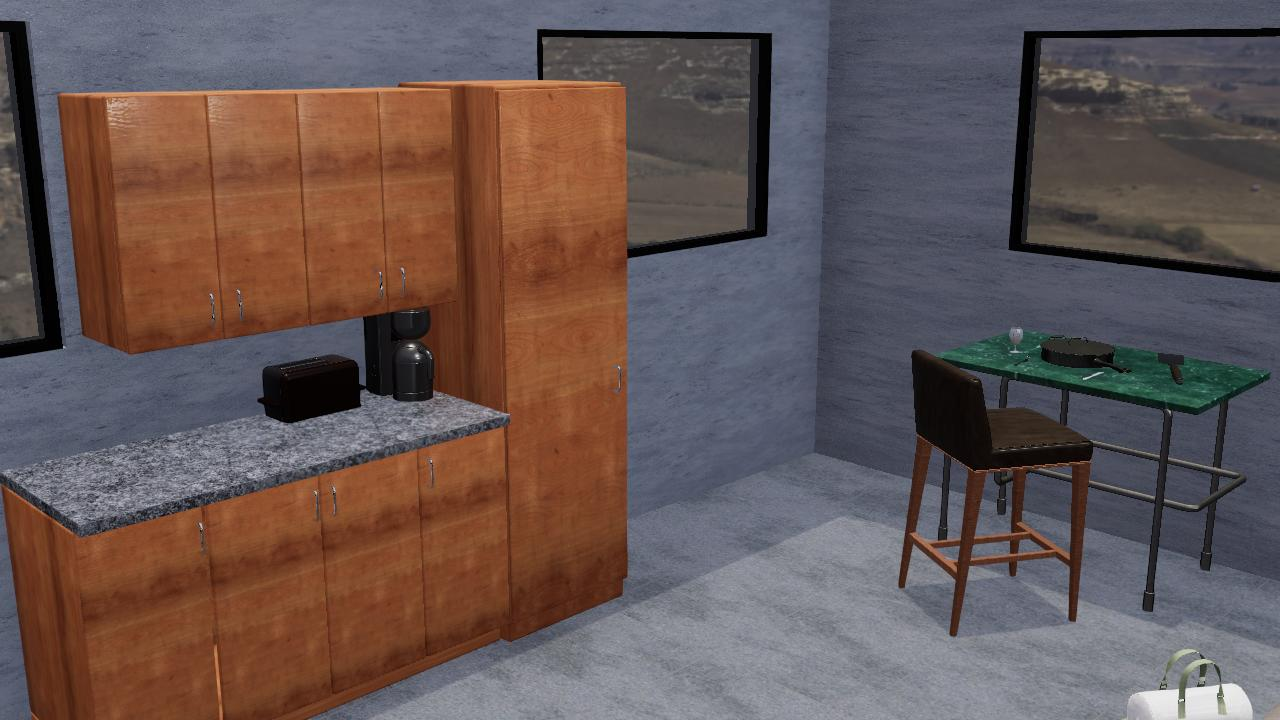
\includegraphics[width=0.19\textwidth]{figures/omnigibson/tdw_sample.jpg}
%     \includegraphics[width=0.19\textwidth]{figures/render_compare_results.png}
%     \includegraphics[width=0.19\textwidth]{figures/render_compare_results.png}
%     \caption{[Comparative][In main body of text] Left: rendering quality example of \simulator, AI2Thor, and ThreeDWorld. Right: we quantify the relative visual realism of \simulator against the other main embodied AI simulators (AI2Thor, ThreeDWorld, Habitat2.0, iGibson2.0) with an AMT study, where subjects were asked to rank randomly sampled images from each simulator in order of realism. We find that \simulator performs XXX \josiah{TODO! Once we have results}.}
%     %\caption{[Comparative][In main body of text] (a) Side-by-side comparison of rendering quality: OmniGibson, OmniGibson-path tracing (super high quality but slow), iGibson, Habitat, AI2. The figures of other benchmarks will come from their demo videos, but OmniGibson will still be visually better than them. (b) Quantitative results for the AMT study showing that OmniGibson is the most realistic judging by humans.}
%     \label{fig:sim_render}
% \end{figure}


% \begin{figure}[h]
% \scalebox{0.96}{
% \captionsetup[subfigure]{labelformat=empty}
% \centering

% \sbox{\bigpicturebox}{%
%   \begin{subfigure}[b]{.49\textwidth}
%   \scalebox{1}[1.2]{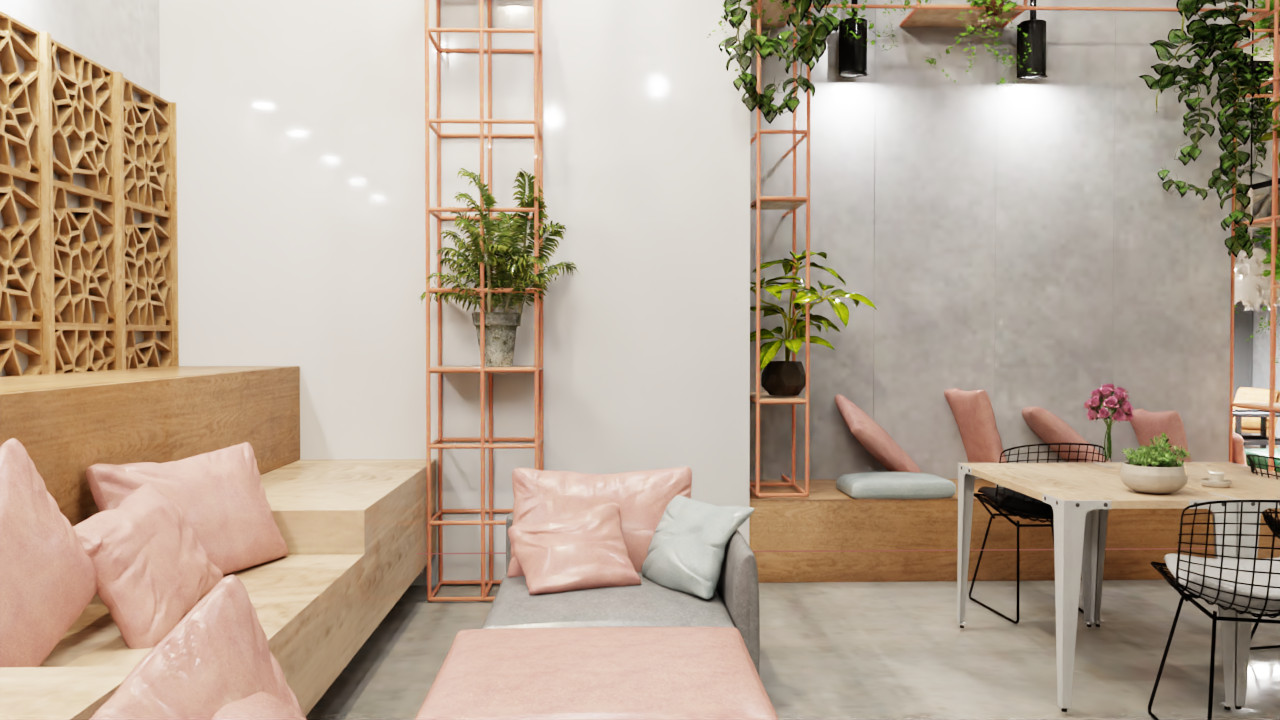
\includegraphics[width=\textwidth]{figures/omnigibson/og_sample.png}}%
% \caption{\textbf{OmniGibson: $\mathbf{1.82\pm1.24}$}}
% \end{subfigure}\hspace{0.3cm}
% }


% \usebox{\bigpicturebox}\hfill
% \begin{minipage}[b][\ht\bigpicturebox][s]{.50\textwidth}
% \begin{subfigure}{.49\textwidth}
% 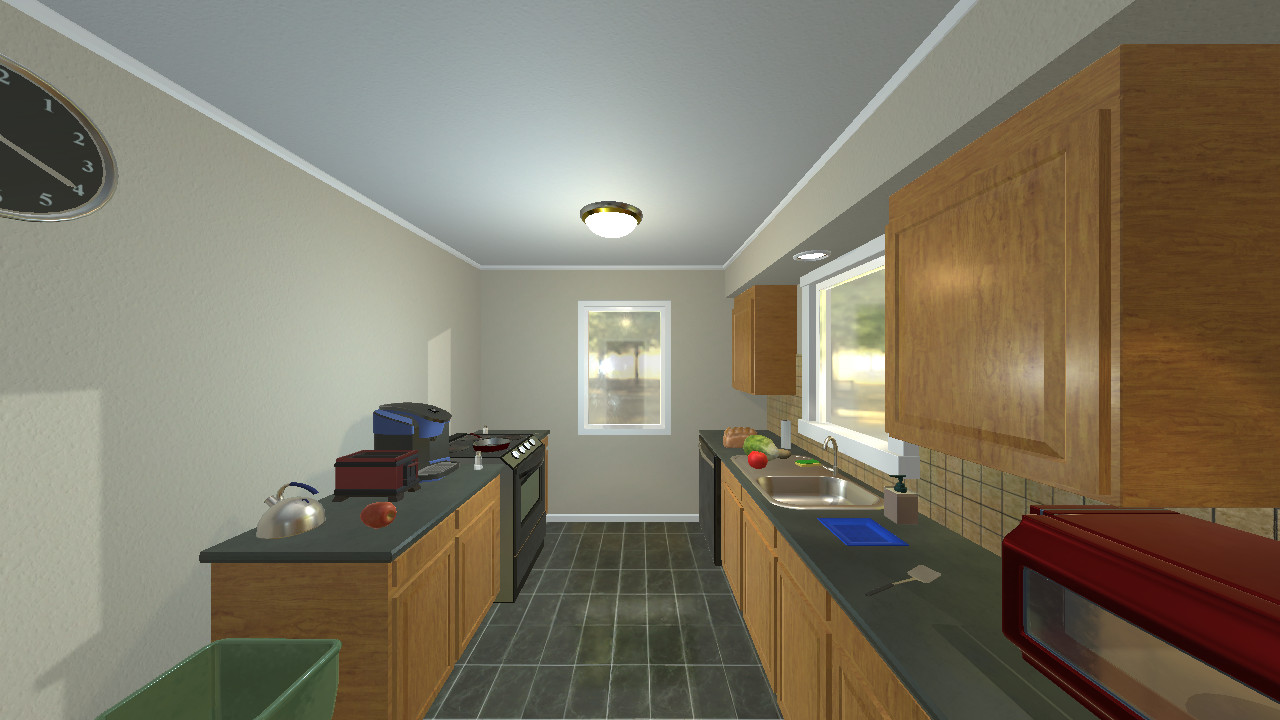
\includegraphics[width=\textwidth]{figures/omnigibson/ai2_sample.png}
% \caption{AI2Thor: $3.27\pm1.25$}
% \end{subfigure}\hfill
% \begin{subfigure}{.49\textwidth}
% 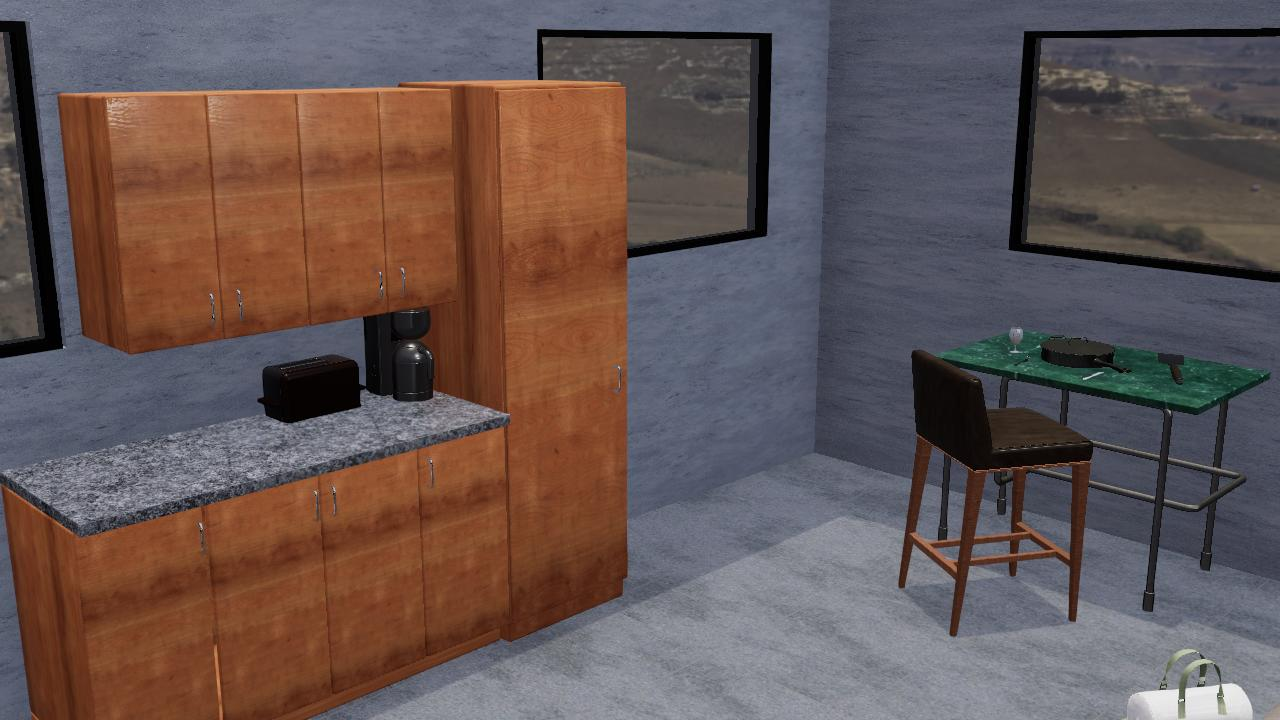
\includegraphics[width=\textwidth]{figures/omnigibson/tdw_sample.jpg}
% \caption{ThreeDWorld: $3.37\pm1.23$}
% \end{subfigure}

% \vfill

% \begin{subfigure}[b]{.49\textwidth}
% 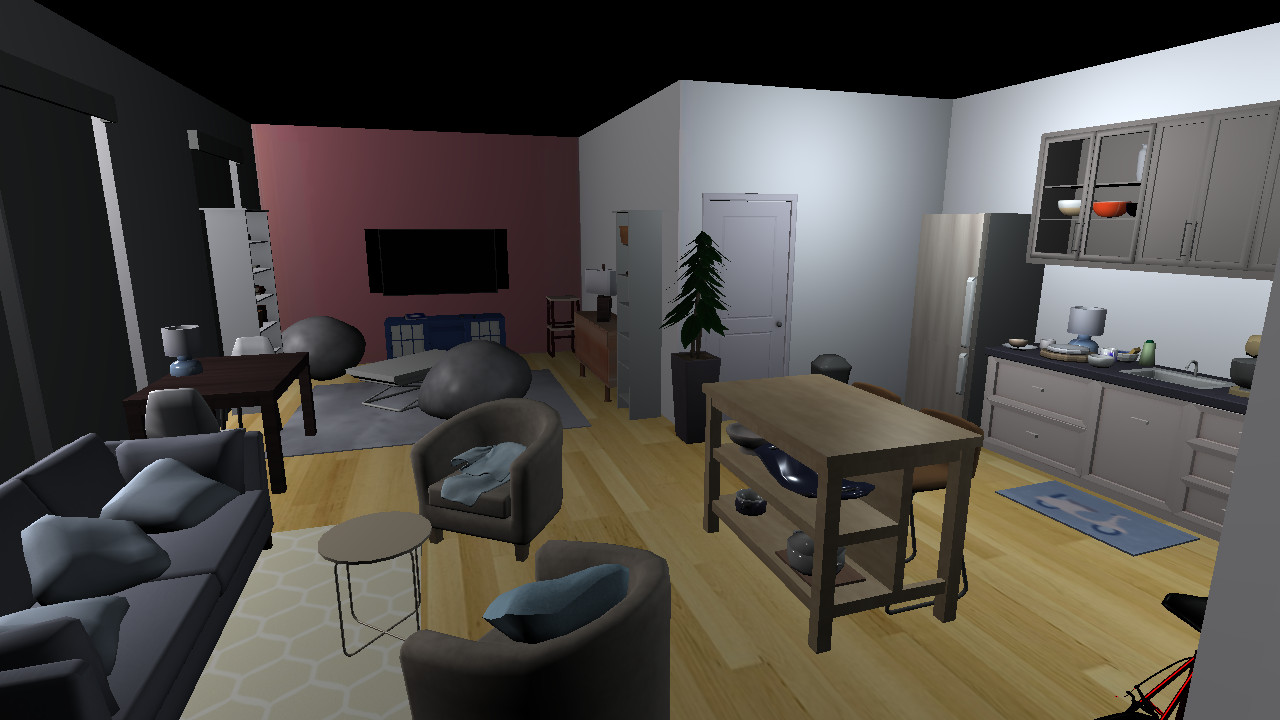
\includegraphics[width=\textwidth]{figures/omnigibson/habitat_sample.png}
% \caption{Habitat2.0: $3.27\pm1.32$}
% \end{subfigure}\hfill
% \begin{subfigure}[b]{.49\textwidth}
% 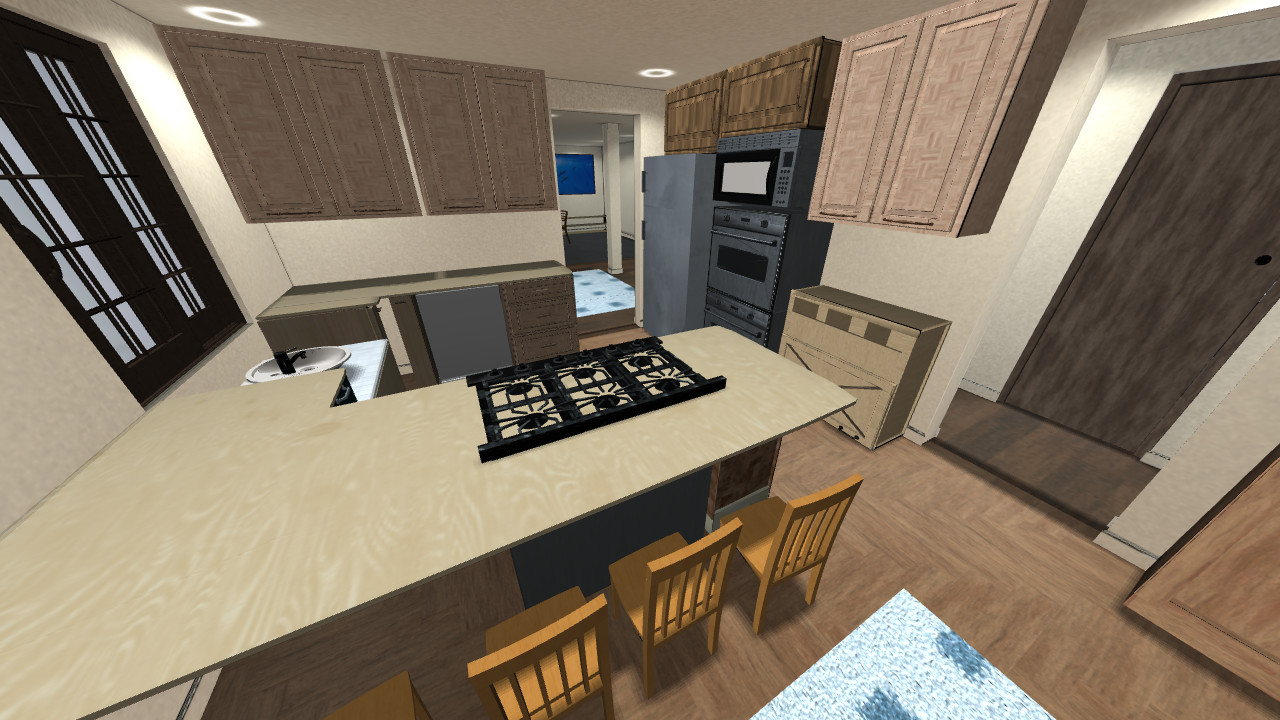
\includegraphics[width=\textwidth]{figures/omnigibson/ig2_sample.png}
% \caption{iGibson2.0: $3.27\pm1.25$}
% \end{subfigure}
% \end{minipage}
% }
% \caption{We evaluate \simulator's visual realism compared to alternative simulation environments by running a survey with 50 human participants to rank the realism of sampled images from each respective environment in order of 1 (most realistic) to 5 (least realistic). We report the resulting mean and standard deviation for each environment, as well as a sampled image from the study, and find that the survey participants consider \simulator to be significantly more realistic compared to all other environments.}

% \label{fig:sim_render}

% \end{figure}


% \sbox{\bigpicturebox}{%
%   \begin{subfigure}[b]{.49\textwidth}
%   \scalebox{1}[1.2]{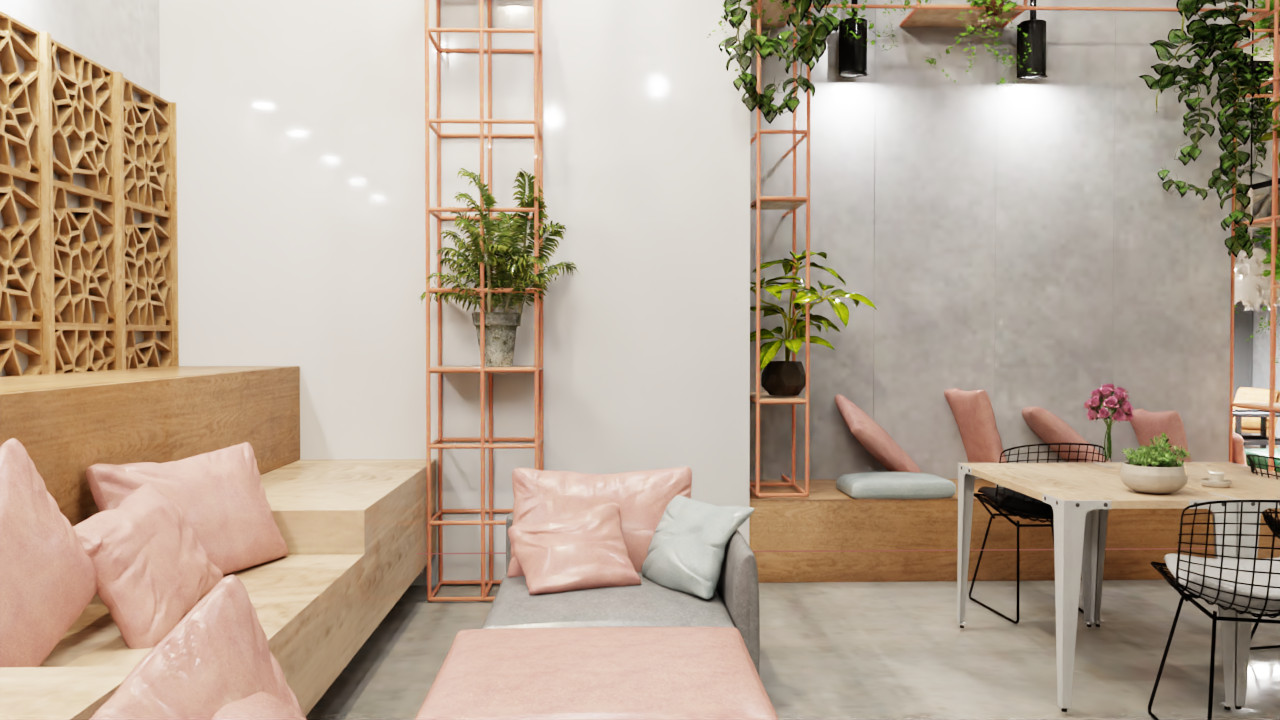
\includegraphics[width=\textwidth]{figures/omnigibson/og_sample.png}}%
% \caption{\textbf{OmniGibson: $\mathbf{1.82\pm1.24}$}}
% \end{subfigure}\hspace{0.3cm}
% }


% \usebox{\bigpicturebox}\hfill
% \begin{minipage}[b][\ht\bigpicturebox][s]{.50\textwidth}
% \begin{subfigure}{.49\textwidth}
% 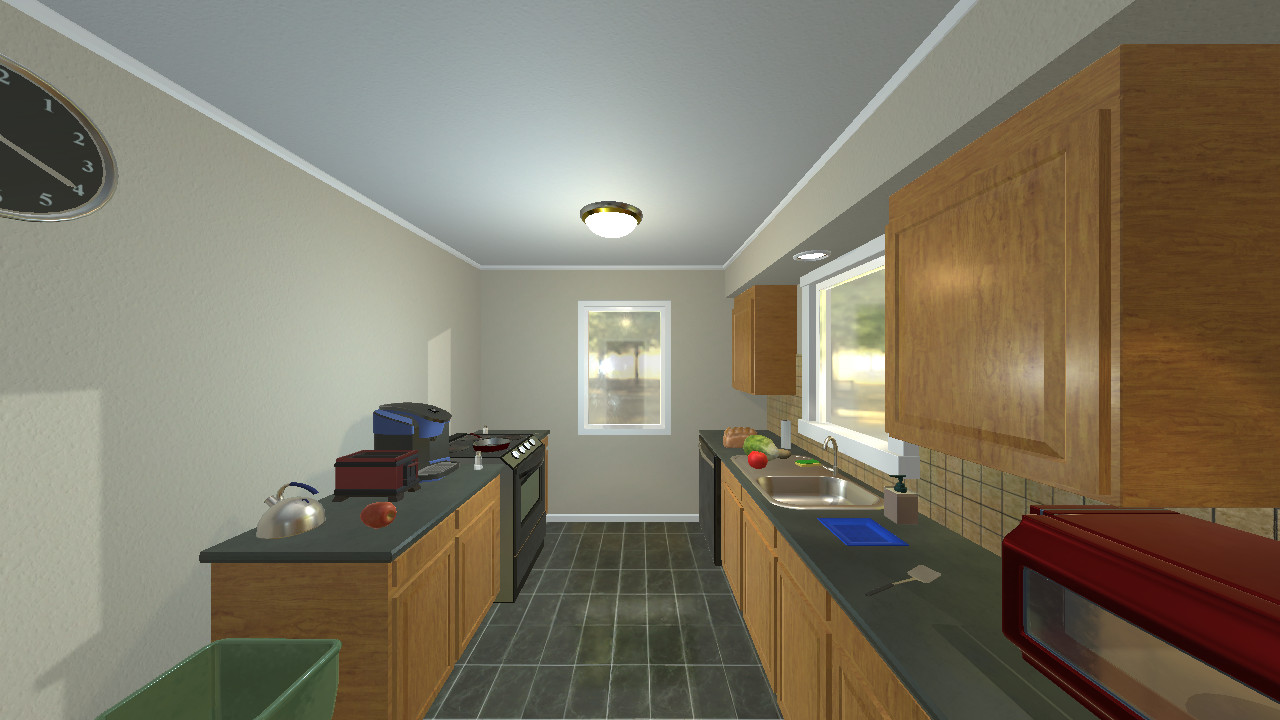
\includegraphics[width=\textwidth]{figures/omnigibson/ai2_sample.png}
% \caption{AI2Thor: $3.27\pm1.25$}
% \end{subfigure}\hfill
% \begin{subfigure}{.49\textwidth}
% 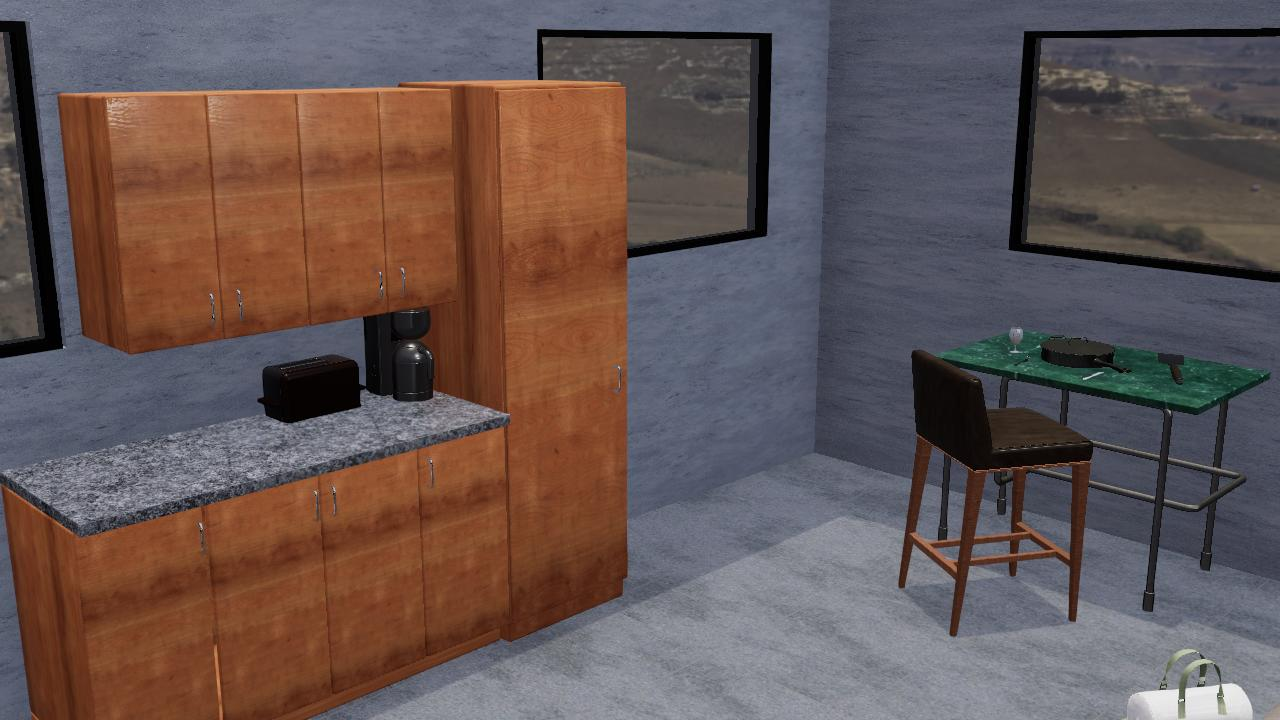
\includegraphics[width=\textwidth]{figures/omnigibson/tdw_sample.jpg}
% \caption{ThreeDWorld: $3.37\pm1.23$}
% \end{subfigure}

% \vfill

% \begin{subfigure}[b]{.49\textwidth}
% 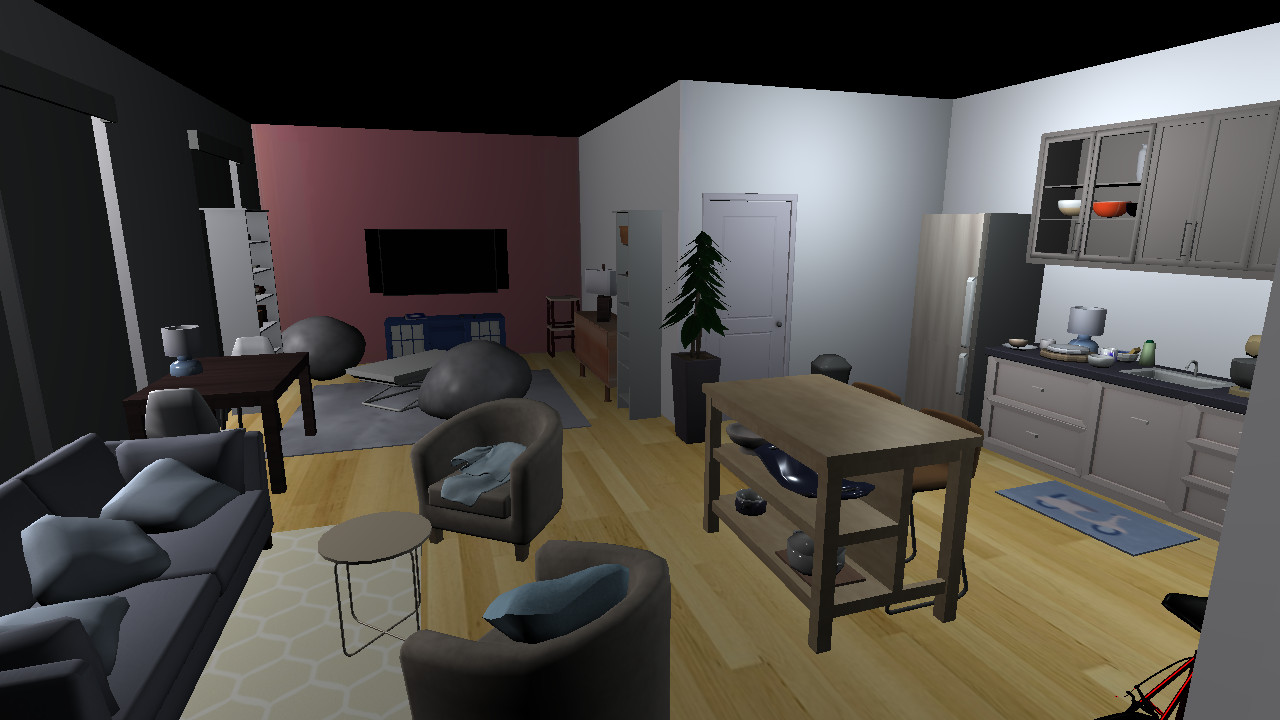
\includegraphics[width=\textwidth]{figures/omnigibson/habitat_sample.png}
% \caption{Habitat2.0: $3.27\pm1.32$}
% \end{subfigure}\hfill
% \begin{subfigure}[b]{.49\textwidth}
% 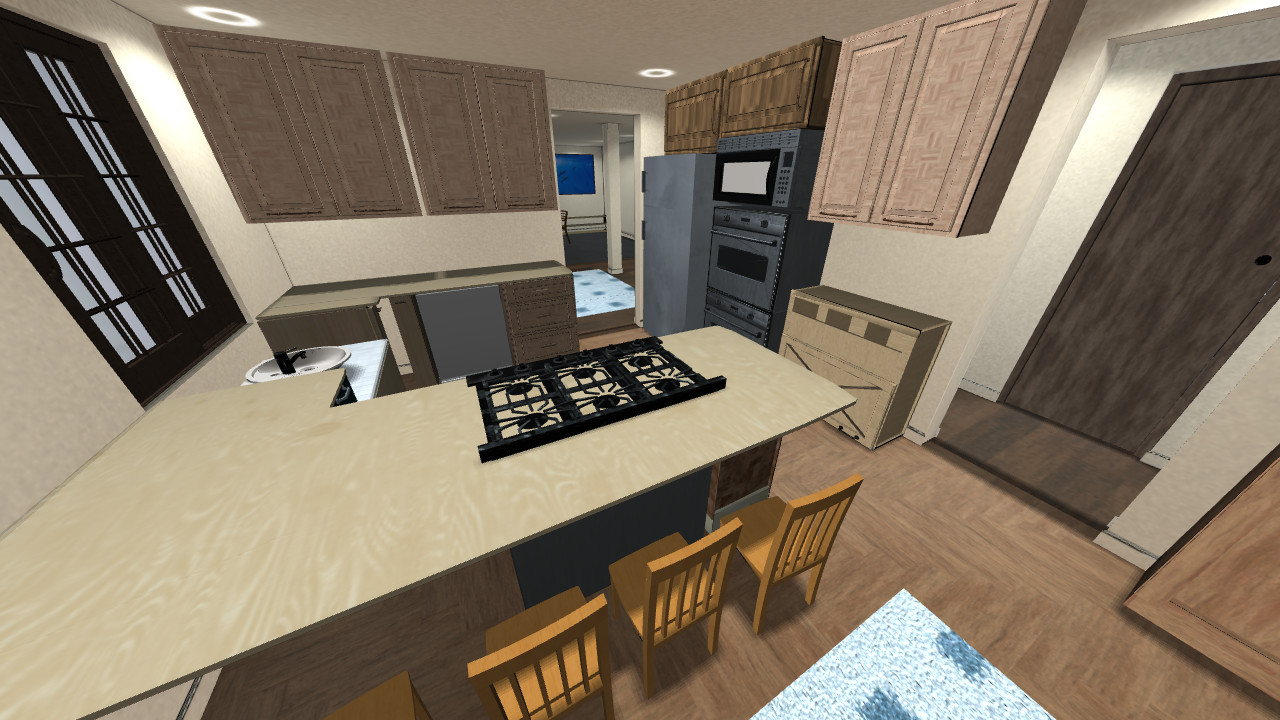
\includegraphics[width=\textwidth]{figures/omnigibson/ig2_sample.png}
% \caption{iGibson2.0: $3.27\pm1.25$}
% \end{subfigure}
% \end{minipage}
% }




% \begin{figure}
% \centering

% \sbox{\bigpicturebox}{%
%   \begin{subfigure}[b]{.45\textwidth}
%   \scalebox{1}[1.2]{\includegraphics[width=\textwidth]{example-image}}%
% \caption{Big picture}
% \end{subfigure}
% }

% \usebox{\bigpicturebox}\hfill
% \begin{minipage}[b][\ht\bigpicturebox][s]{.45\textwidth}
% \begin{subfigure}{.45\textwidth}
% \includegraphics[width=\textwidth]{example-image-a}
% \caption{Small figure}
% \end{subfigure}\hfill
% \begin{subfigure}{.45\textwidth}
% \includegraphics[width=\textwidth]{example-image-b}
% \caption{Small figure}
% \end{subfigure}

% \vfill

% % \begin{subfigure}[b]{.45\textwidth}
% % \includegraphics[width=\textwidth]{example-image-c}
% % \caption{Small figure}
% % \end{subfigure}


% \begin{subfigure}[b]{.45\textwidth}
% \includegraphics[width=\textwidth]{example-image-a}
% \caption{Small figure}
% \end{subfigure}\hfill
% \begin{subfigure}[b]{.45\textwidth}
% \includegraphics[width=\textwidth]{example-image-b}
% \caption{Small figure}
% \end{subfigure}

% \end{minipage}

% \end{figure}



% To conclude, \simulator is a realistic simulator that supports a set of diverse features required to simulate \benchmark activities (see Fig.~\ref{fig:sim_obj_prop}). Although OmniGibson is the only simulator that can support B1K now, in the future, B1K is simulator agnostic and can be implemented in other simulators. 

\begin{figure}[t]
    \centering
    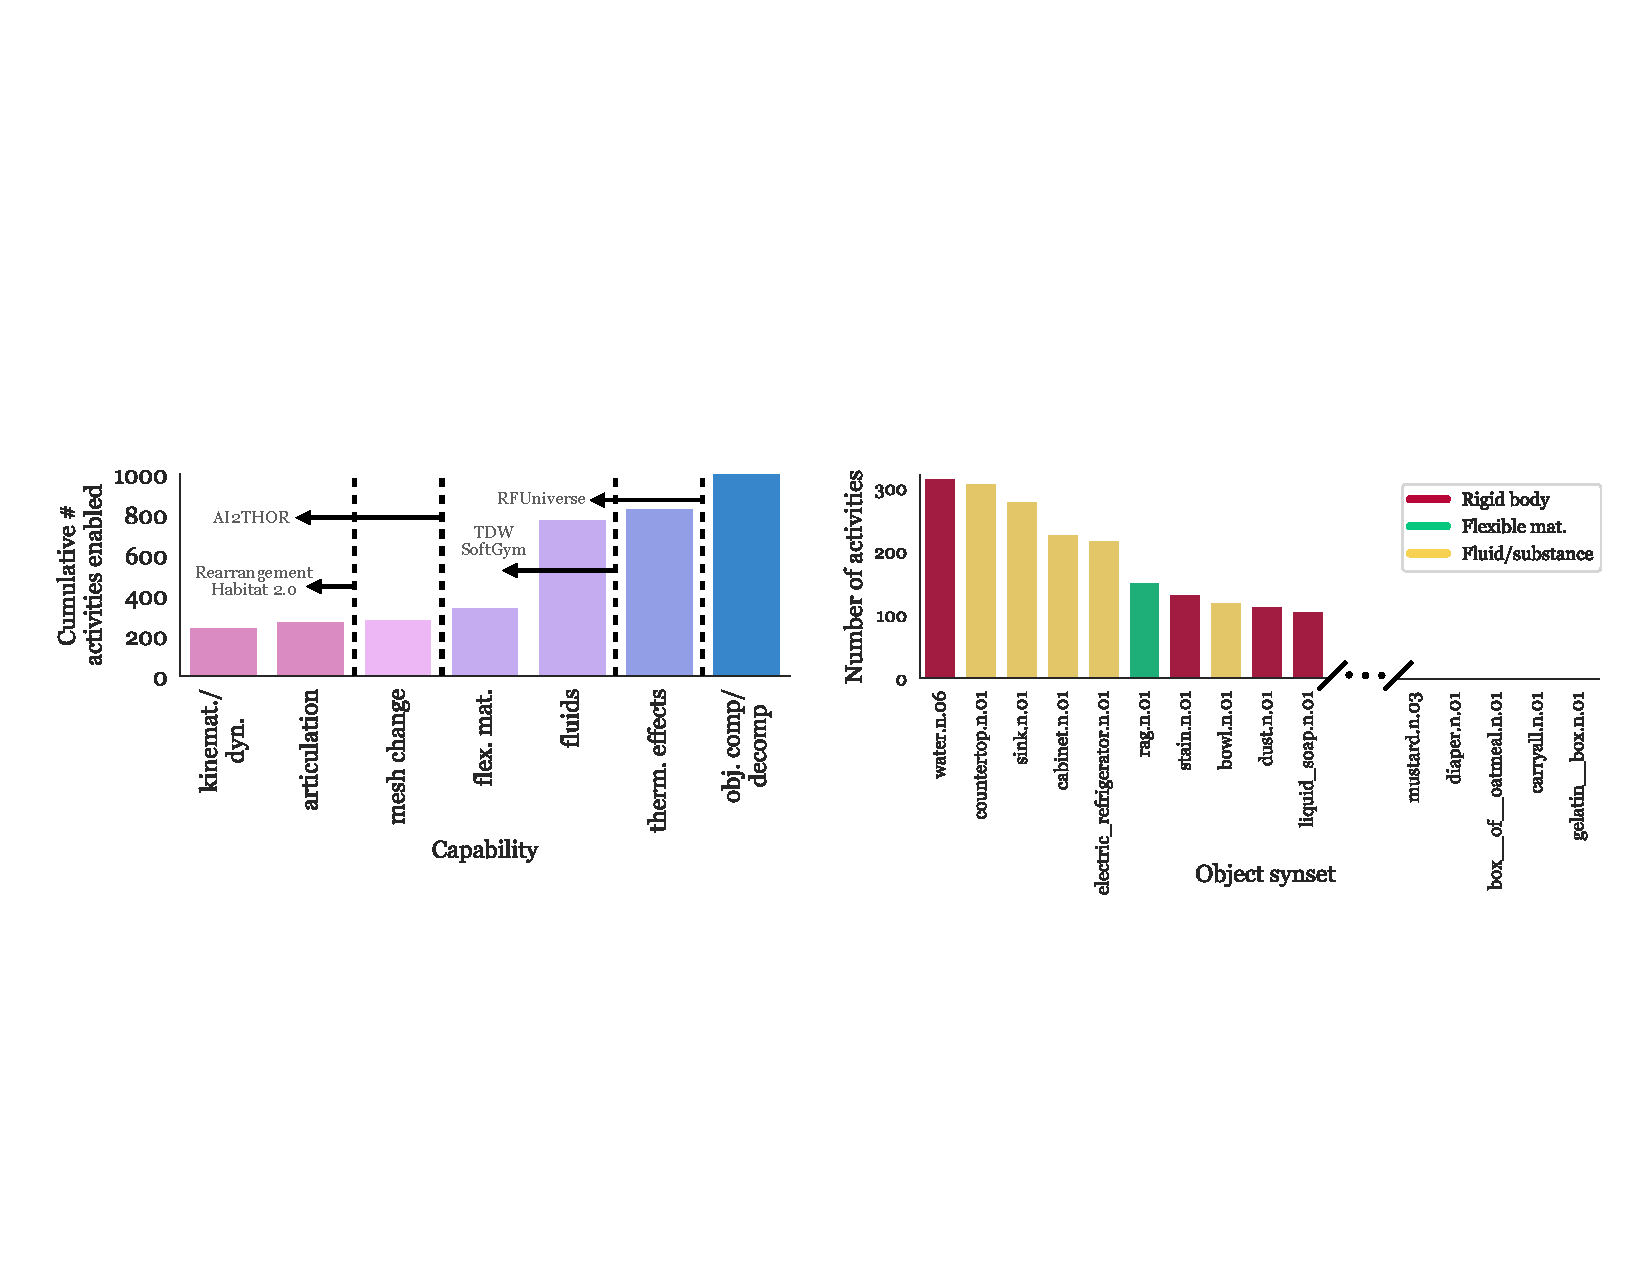
\includegraphics[width=1\textwidth]{figures/object-activity-figs-2024.pdf}\\
    \caption{\textbf{Objects and States in Activity Definitions:} Left: the number of activities unlocked by each simulation capability that \simulator has. None of the other simulation environments are sufficient to fully support \benchmark, e.g. Habitat 2.0 can support only 23\% of the activities. Right: the number of activities that require each object synset (category). Several top-10 object synsets are fluids and flexible materials, necessitating the development of \simulator. As we expect, the object synsets also follow a long-tail distribution: most objects are involved in only a few activities.}
    \vspace{10pt}
    \label{fig:sim_obj_prop}
\end{figure}


\section{Experiments: Evaluating Embodied AI Solutions in \benchmark}
\label{sec:baseline}


In our experiments, we aim to answer three questions: How do existing vision-based robot learning algorithms perform in \benchmark, and what assumptions have to be made to improve their success? What elements of the activities are the most problematic for current AI? What are the main sources of the sim-real gap in \benchmark/\simulator? Our goal is to indicate promising research directions to improve AI's performance in \benchmark activities in simulation and, ultimately, in the real world.

%How important is each technical components for training a successful home robot? 4) How could training the agent in a realistic simulated environment help solving real world robot manipulation tasks?

\subsection{Evaluating \benchmark Solutions in \simulator}
\label{ss:ev_in_sim}

%\paragraph{Activities:} 
% To gain insights on the difficulties associated to characteristics of the \textbf{activities}, w
\paragraph{Experimental Setups.} We selected three paradigmatic activities for our experiments: 
\texttt{CollectTrash}, where the agent gathers empty bottles and cups, and throws them into a trash bin (rigid body manipulation); \texttt{StoreDecoration}, where the agent stores items into a drawer (articulated object manipulation); and \texttt{CleanTable}, where the agent wipes a dirty table with a soaked piece of cloth (manipulation of flexible materials and fluids). 
% Each activity takes place in a different scene: living rooms of different apartments, and a restaurant. 
% All three activities are defined using BDDL that provides a sparse final success signal as the reward function to train the policy.
We evaluate three different baselines based on state-of-the-art reinforcement learning algorithms (RL)~\cite{barto2003recent}: 
\begin{itemize}
    \item \rlvmc, a visuomotor control (from image to low-level joint commands) RL solution based on Soft Actor-Critic (SAC)~\cite{haarnoja2018soft};
    \item \rlprim, a RL solution based on PPO~\cite{schulman2017proximal} that leverages a set of action primitives based on a sampling-based motion planner~\cite{lavalle2006planning,kuffner2000rrt,Jordan.Perez.ea:CSAIL13} (\texttt{pick}, \texttt{place}, \texttt{push}, \texttt{navigate}, \texttt{dip} and \texttt{wipe}). The policy outputs a discrete selection of a primitive applied on an object;
    \item \rlprimhist, a variant of \rlprim that takes in the history observations (3 steps) as additional inputs to help disentangle similar-looking states.    
\end{itemize} 

All agents are trained with a sparse task success reward without any reward engineering. Following the metrics proposed in \oldbenchmark~\cite{srivastava2021behavior}, we report the success rate and efficiency metrics (distance traveled, time invested, and disarrangement caused) in Table~\ref{tab:baseline_performance} and~\ref{tab:baseline_metric}, and the success score Q in Table~\ref{tab:baseline_q_score} in Appendix. 

\begin{table}[t]
    \centering
    \resizebox{\textwidth}{!}{\begin{tabular}{l|cc|ccc}
    \toprule
    \multicolumn{1}{c|}{\multirow{2}{*}{Method}} & \multicolumn{2}{c|}{Policy Features} & \multicolumn{3}{c}{Task success rate} \\
    \multicolumn{1}{c|}{} & Primitives & History & \texttt{StoreDecoration} & \texttt{CollectTrash} & \texttt{CleanTable} \\ \midrule
    \rlvmc & \textcolor{red}\faTimes & \textcolor{red}\faTimes & $0.0 \pm 0.0$ & $0.0 \pm 0.0$ & $0.0 \pm 0.0$ \\
    \rlprim & \textcolor{indiagreen}\faCheck & \textcolor{red}\faTimes & $0.48 \pm 0.06$ & $0.42 \pm 0.02$ & $0.77 \pm 0.08$ \\
    \rlprimhist & \textcolor{indiagreen}\faCheck & \textcolor{indiagreen}\faCheck & $0.55 \pm 0.05$ & $0.63 \pm 0.03$ & $0.88 \pm 0.02$ \\ \bottomrule
    \end{tabular}
    }
    \caption{Task success rates across three baseline methods. \rlvmc with end-to-end visuomotor control completely fails to solve any of the activities, whereas \rlprim and \rlprimhist with action primitives are able achieve decent performance. Memory of observations helps in longer horizon activities (e.g. \texttt{CollectTrash}).}
    \label{tab:baseline_performance}
\end{table}

% RL has demonstrated success in learning mappings from robot's observations to actions to achieve embodied AI tasks~\cite{robomimic2021}. We evaluated a visuomotor control (from image to low-level joint commands) RL solution based on Soft Actor-Critic (SAC)~\cite{haarnoja2018soft} on the aforementioned activities (\rlvmc). Similar to what has been observed with other end-to-end RL algorithms, without costly reward engineering~\cite{fu2018learning}, SAC cannot solve these long-horizon mobile manipulation activities due to problems such as credit assignment~\cite{alipov2021towards}, deep exploration~\cite{yang2021exploration,JMLR:v20:18-339}, and vanishing gradients~\cite{10.1142/S0218488598000094}. To alleviate the challenge of long-horizon, we implemented a set of action primitives based on a sampling-based motion planner~\ref{lavalle2006planning,kuffner2000rrt,Jordan.Perez.ea:CSAIL13}: \textit{Pick}, \textit{Place}, \textit{Push}, \textit{Toggle}, \textit{Navigate}, \textit{Dip} and \textit{Wipe}. We trained a RL agent using Proximal Policy Optimization (PPO)~\cite{schulman2017proximal} in the discrete action space action primitives on objects (\rlprim). Even with the help of action primitives, some \benchmark activities require more 20 steps and several of the phases of the activity look visually similar. We hypothesize that a memory mechanism can help  disentangling these states and identifying the different phases. We evaluated a variant of the primitive-based agent with history of previous actions (\rlprimhist) to analyze the effect of agent's memory on task success.

%\paragraph{Simplifying Physics and Actuation during Training.} 
Grasping is a challenging research topic on its own. To facilitate our experiments, we adopt an assistive \texttt{pick} primitive that creates a rigid connection between the object and the gripper if grasping is requested when all fingers are in contact with the object, a stricter form of \textit{StickyMitten} used in prior works~\cite{szot2021habitat, ehsani2021manipulathor, li2020hrl4in}. Furthermore, to accelerate training, %Due to the complex scenes and processes involved, \simulator currently achieves around 50 fps. We accelerate planning, simulation and rendering for training, by 
the action primitives check only the feasibility (e.g., reachability, collisions) of the final configuration, e.g. the grasping pose for \texttt{pick} or the desired location for \texttt{navigate}. If kinematically feasible, the action primitives will directly set the robot state to the final configuration, and continue to simulate from then on. We include an ablation analysis of the effect of these assumptions and simplifications in our evaluation (see Table~\ref{tab:baseline_ablation}).
%The effect of these assumptions on the model performance is studied in Table.\ref{tab:baseline_ablation}.
Further details about our training and evaluation setup can be found in Appendix~\ref{sec:baseline_appendix}.

% Activating full-physics grasping (the use of assistive grasping must be explained before, in the conditions of the "normal" run)
% Activating full-path physics (the use of "teleportation" must be explained before, in the conditions of the "normal" run)

%\subsection{Results}
\paragraph{Results: Task Completion.} Table~\ref{tab:baseline_performance} contains task success rates across our baseline methods. The extreme long-horizon in our activities causes the visuomotor control (RL-VMC) policy to fail in all three activities, potentially due to problems such as credit assignment~\cite{alipov2021towards}, deep exploration~\cite{yang2021exploration,JMLR:v20:18-339}, and vanishing gradients~\cite{10.1142/S0218488598000094} as reported by prior works.
Our baselines with time-extended action primitives (\rlprim and \rlprimhist) obtain better success, achieving over 40\% success rates across all three activities. We observe that longer-horizon activities are more challenging: while \texttt{CleanTable} can be accomplished by executing the optimal sequence of 6 primitive steps, \texttt{CollectTrash} requires at least $16$.
This supports the idea that some form of action-space abstraction must be necessary to solve long-horizon activities of \benchmark, as others reported~\cite{srivastava2021behavior, szot2021habitat,xia2020relmogen}.
% \paragraph{\benchmark activities are challenging for end-to-end visuo-motor control RL algorithms:} In  we show the experimental results of all baseline methods in the three activities.  With the access to action primitives, \rlprim achieves $>$40\% success rate in all three activities. We observe that the activities with longer-horizon are more challenging, comparing the results of \texttt{clean\_table} (requires at least $6$ primitive steps) to \texttt{collect\_trash} (require at least $16$ primitive steps).
% \paragraph{Temporal information is crucial for long-horizon \benchmark activities:} 
When analyzing the role of memory, we observe a sizable performance gain from \rlprim to \rlprimhist, especially in long-horizon activities with aliased observations such as \texttt{CollectTrash}. In this task, when the robot is looking at the trash bin, it needs additional information to know what location has been cleaned already in order to proceed to other locations.
Our results indicate that memory will play a critical role for embodied AI in long-horizon \benchmark activities.
% like \texttt{collect\_trash} with up to $\times$3 more improvement than in short-horizon activities like \texttt{store\_halloween}.

\paragraph{Results: Efficiency.} In addition to success, efficiency is also critical in the evaluation of embodied AI: a successful policy in simulation may be infeasible in the real world if it takes a long time or wastes too much energy. In Table~\ref{tab:baseline_metric}, we report the results with three efficiency metrics proposed by Srivastava et al.~\cite{srivastava2021behavior}. We observe that the use of memory (\rlprimhist) improves efficiency across all metrics: distance navigated (Dist.~Nav.), simulated time (Sim.~Time), and kinematic object disarrangement (Kin.~Dis.), i.e., amount of object displacement due to robot motion.%Analysis of additional metrics such as the fraction of activity achieved (Q) can be found in Appendix.
%\rlvmc has the worst spatial and time efficiency because it cannot learn meaningful behaviors and constantly move around with at no avail. 

We also evaluate to what extent the simplifications we introduce in physics and actuation (grasping, motion execution) during training impact the performance of \rlprim during evaluation when these simplifications are removed. We report the results in Table~\ref{tab:baseline_ablation}. 
% We evaluate the performance of \rlprim with fully physically-simulated grasping and motion trajectories and reports the results in Table.~\ref{tab:baseline_ablation}. 
We observe a radical performance drop after enabling fully physics-based grasping during evaluation. Grasping is thus a critical component of any embodied AI task, and researchers should be careful when simplifying its execution during training. While \simulator supports fully physics-based grasping,  designing a \texttt{pick} action primitive for arbitrary objects that leverages fully physics-based grasping is by itself an open research problem that we leave for future work. In contrast, there is much less performance drop after enabling full trajectory motion execution during evaluation. This result supports our hypothesis that it is reasonable to accelerate the training process by assuming that motion planning is likely to provide viable paths in free space during evaluation.

\begin{table}[t]
\centering
\begin{minipage}[t]{.41\linewidth}%
\resizebox{\textwidth}{!}{%
\begin{tabular}{l|ccc}%
\toprule
\multicolumn{1}{c|}{\multirow{2}{*}{Method}} & \multicolumn{3}{c}{Metrics in \texttt{CollectTrash}} \\
\multicolumn{1}{c|}{} & Dist. Nav. [m] & Sim. Time [s] & Kin. Dis. [m] \\ \midrule
\rlvmc & $27.58 \pm 5.95$  & $16.67 \pm 0.00$ & $0.00 \pm 0.00$ \\
\rlprim & $17.98 \pm 2.35$ & $13.95 \pm 5.14$ & $12.34 \pm 5.01$  \\
\rlprimhist & $15.33 \pm 2.70$  & $12.48 \pm 3.68$  & $10.82 \pm 3.90$  \\ \bottomrule
\end{tabular}}
\caption{Efficiency metrics across three baseline methods. \rlvmc has low spatial and temporal efficiency because it fails to learn, whereas history information helps remove redundant actions and improve efficiency.}
\label{tab:baseline_metric}%
\end{minipage}%
\hfill
\begin{minipage}[t]{.56\linewidth}%
\resizebox{\textwidth}{!}{%
\begin{tabular}{cc|ccc}%
\toprule
\multicolumn{2}{c|}{Phys. Realism} & \multicolumn{3}{c}{Task success rate} \\
Grasping & Full Motion & \texttt{StoreDecoration} & \texttt{CollectTrash} & \texttt{CleanTable} \\ \midrule
\textcolor{indiagreen}\faCheck & \textcolor{indiagreen}\faCheck & $0.0 \pm 0.0$ & $0.0 \pm 0.0$ & $0.0 \pm 0.0$ \\
\textcolor{red}\faTimes & \textcolor{indiagreen}\faCheck & $0.46 \pm 0.04$ & $0.36 \pm 0.08$ & $0.73 \pm 0.03$ \\ 
\textcolor{red}\faTimes & \textcolor{red}\faTimes & $0.48 \pm 0.06$ & $0.42 \pm 0.02$ & $0.77 \pm 0.08$ \\ \bottomrule
\end{tabular}}
\caption{Ablation study of \rlprim on the impact of removing the simplifying assumptions of grasping and motion execution during evaluation. We observe a large drop in performance when enabling fully physics-based grasping, but not when enabling full trajectory motion execution.}
\label{tab:baseline_ablation}
\end{minipage}
\vspace{10pt}
\end{table}

% \begin{enumerate}
%     \item B1K is a challenging benchmark, solving these 1K activities may require years of effort. Here we make an initial attempt to tackle a few (10) B1K activities, discuss the insight gained, and provide starting code for follow-up research. 
%     \item Task settings: including how we define reward function based on BDDL activity definition and how we configure the learning agents (Fig.~\ref{fig:baseline_task}).
%     \item Our baseline methods and assumptions: end-to-end RL (image+proprioception), skill-based RL, and parameterized skill-based RL (both with pre-mapping). We will use visuals to help explain these methods (Fig.~\ref{fig:baseline_methods}).
%     \item We discuss their performance and insight:
%         \begin{enumerate}
%             \item Overall, how well do these methods work and why (Table \ref{tab:baseline_performance})? 
%             \item The increase in sample efficiency due to skill parameterization.
%             \item The challenge of sparse reward, including suboptimal policy caused by local minima in the reward function. 
%             \item The challenge of manipulating deformable objects.
%         \end{enumerate}
% \end{enumerate}
\subsection{Evaluating \benchmark Solutions on a Real Robot}
% Demonstrating realism
\label{sec:sim2real}

\begin{figure}[t!]
    \centering
    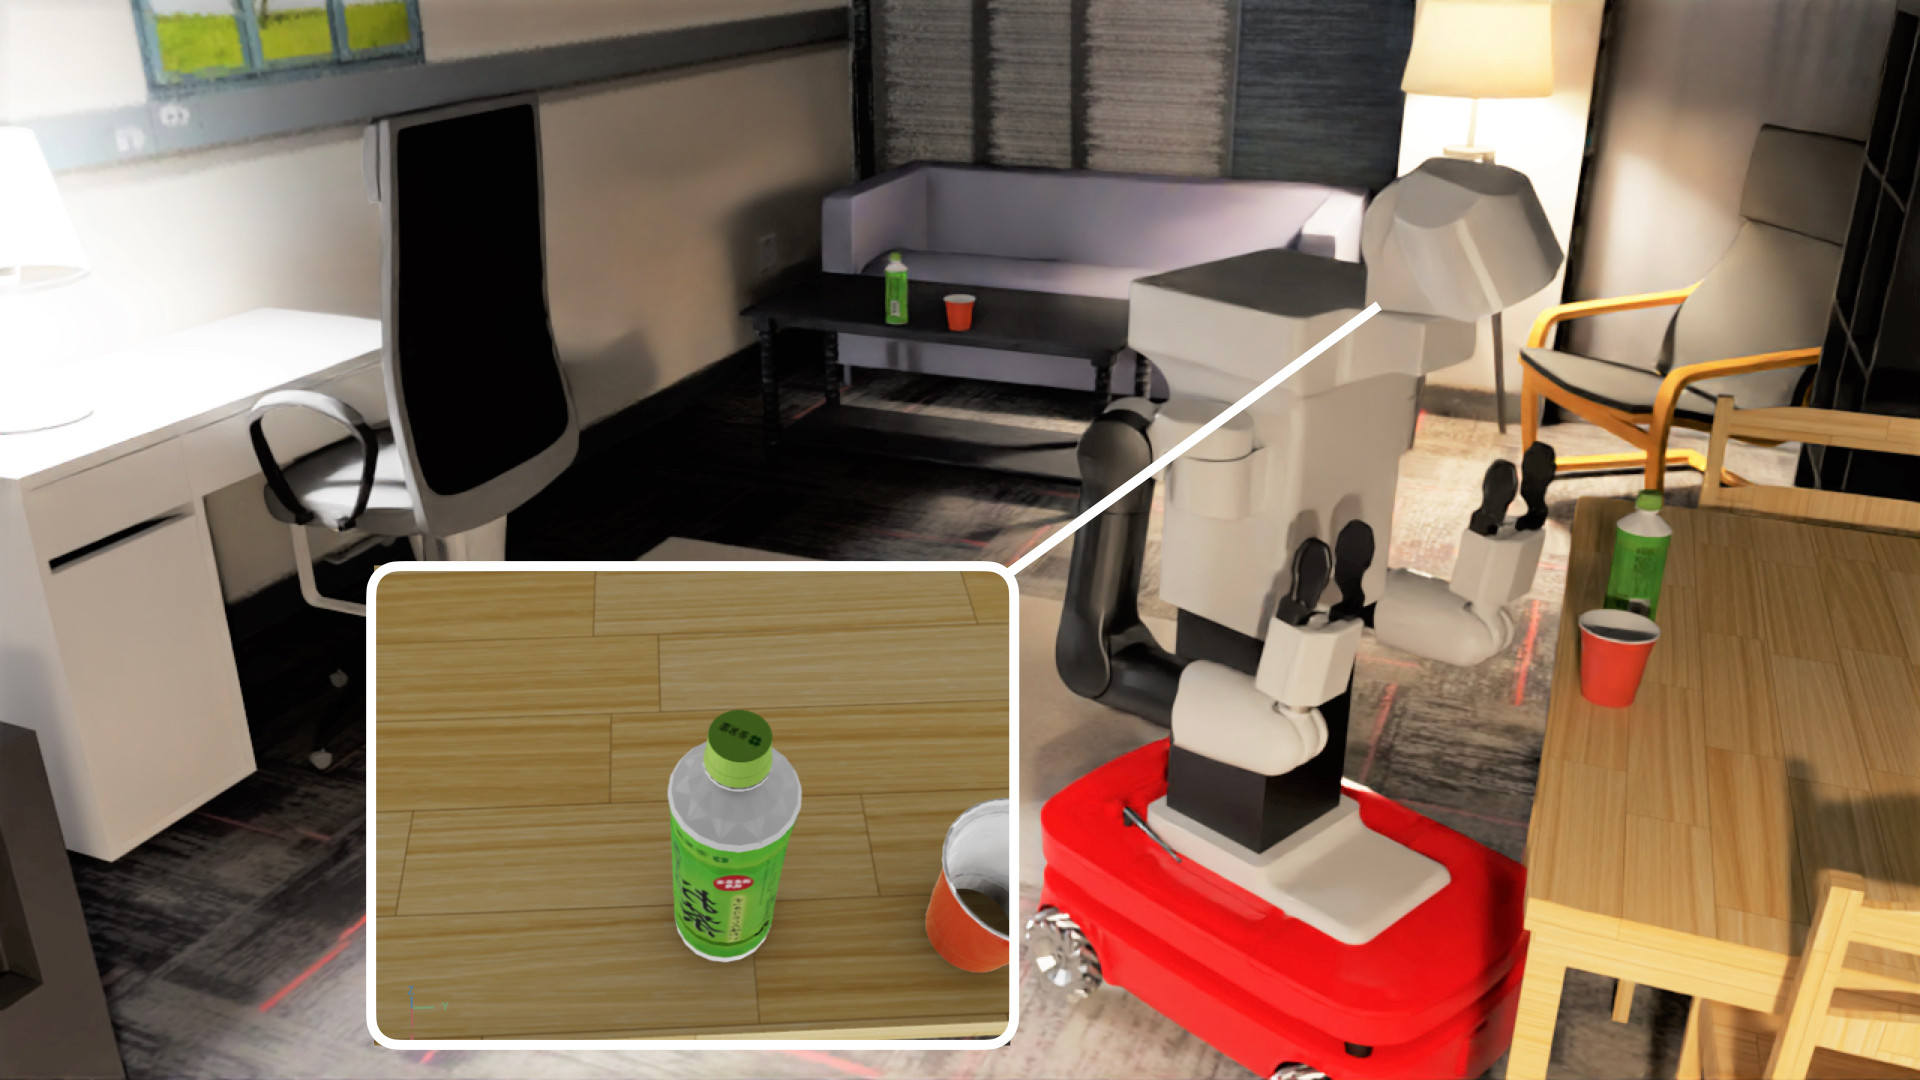
\includegraphics[width=0.27\textwidth,valign=c]{figures/sim2real/sim.001.jpeg}
    \hfill
    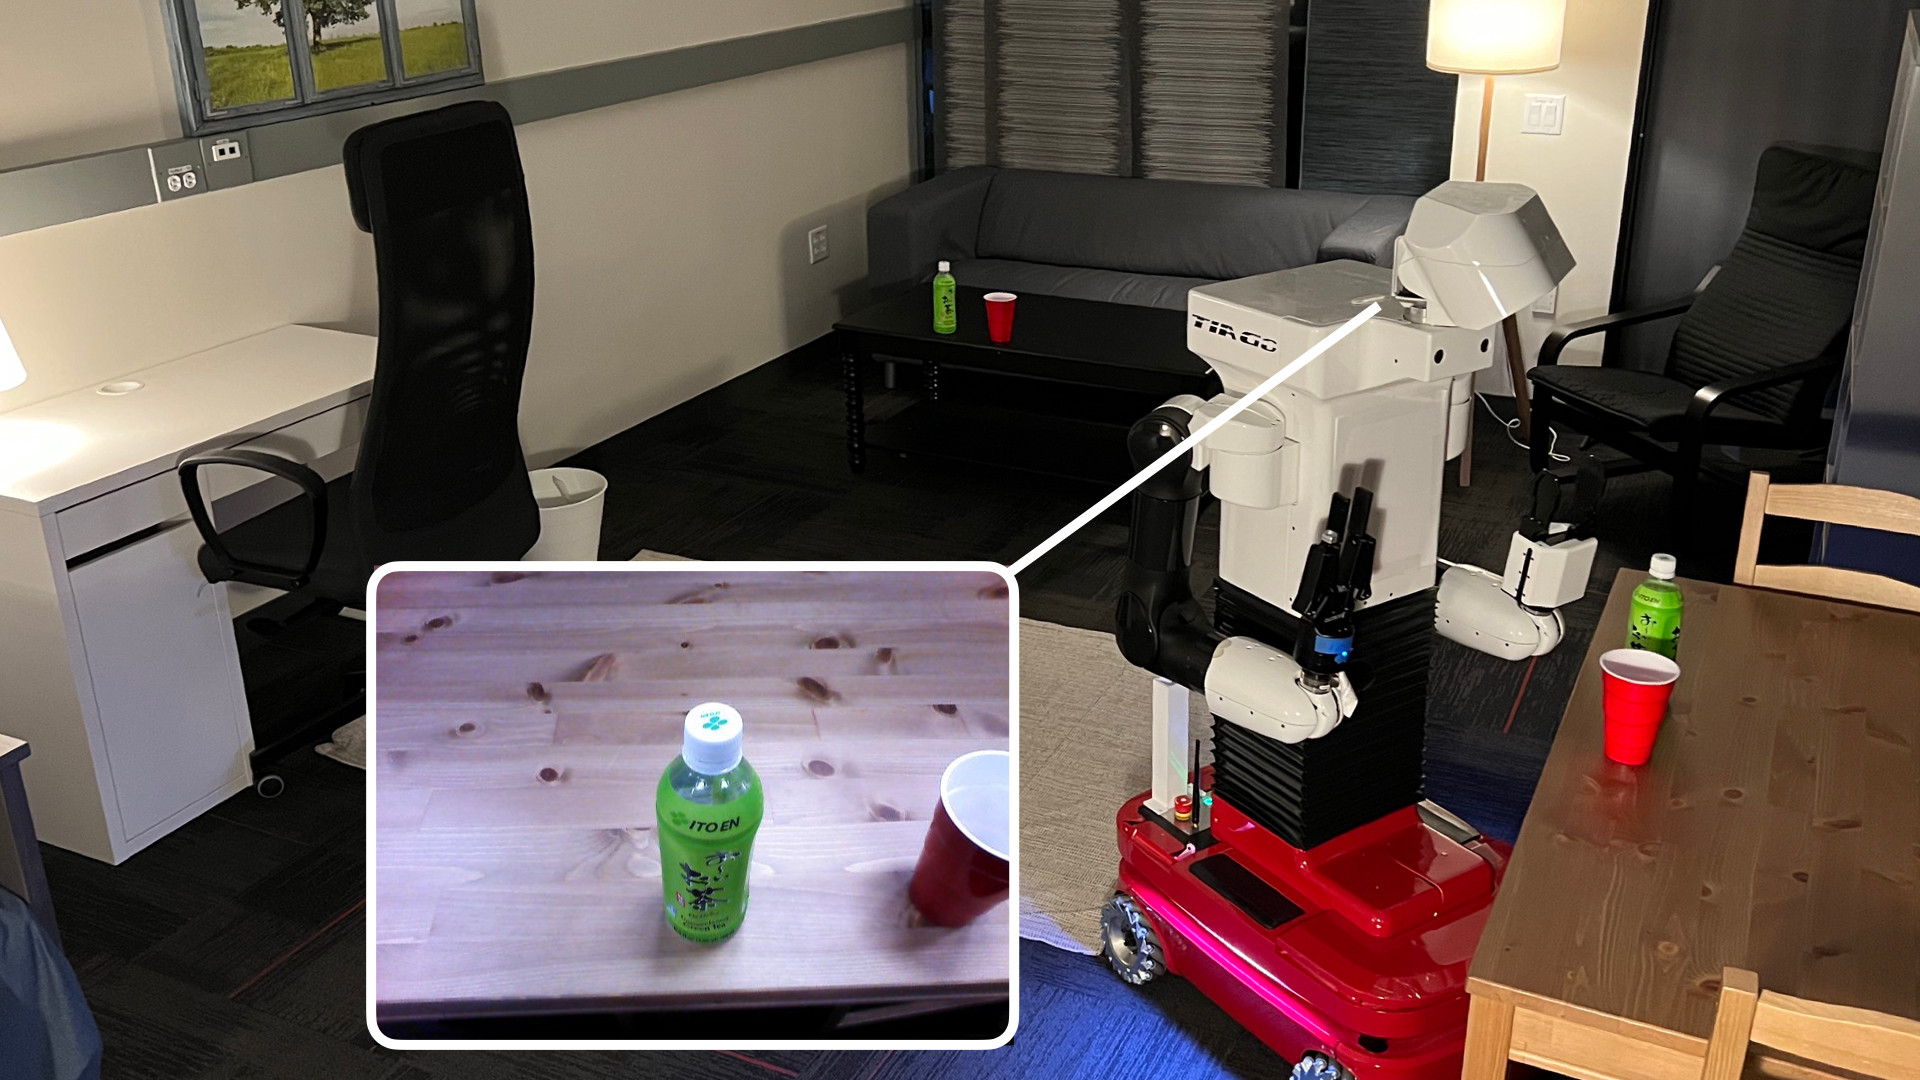
\includegraphics[width=0.27\textwidth,valign=c]{figures/sim2real/real.001.jpeg}
    \hfill
    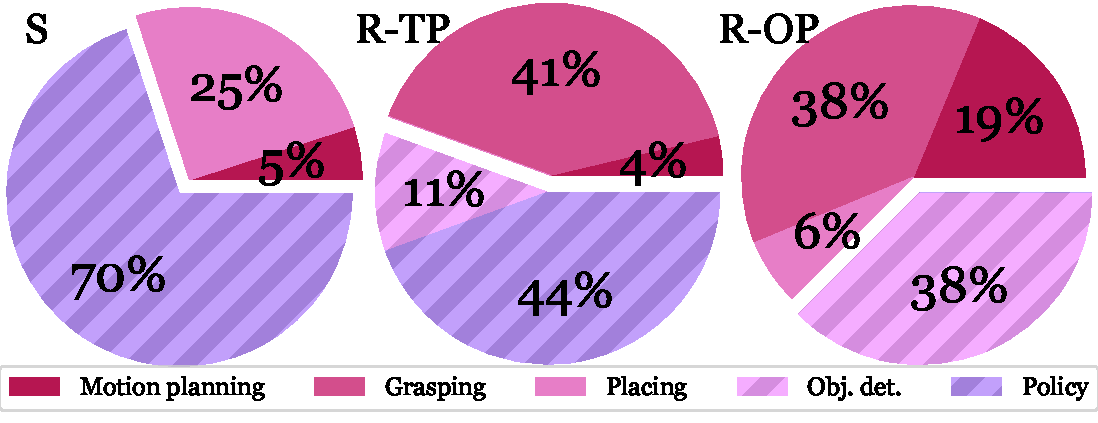
\includegraphics[width=0.44\textwidth,valign=c]{figures/sim2real/error_plot.pdf}
    \caption{\textbf{Characterizing the Sim-Real Gap:} Left: a side-by-side comparison of the simulated and the real scene, including virtual and real images obtained by the robot. While the high-resolution images are extremely similar, the mismatch in wooden texture and camera properties causes a sizable gap in the visual input to the agent. Right: source of failure in \texttt{S}imulation (\texttt{S}, left) and in \texttt{R}eal-world with a \texttt{T}rained \texttt{P}olicy in \simulator (\texttt{R-TP}, middle) and an \texttt{O}ptimal \texttt{P}olicy (\texttt{R-OP}, right) due to actuation (solid color) or perception (striped). In simulation, without full simulation of grasping (see Sec.~\ref{ss:ev_in_sim}), policy failures (i.e., selecting the wrong action primitive) dominate. On the real robot, grasping is one of the main causes of error, as well as perception issues (policy errors with the trained visual policy, object detection errors with the optimal policy).}
    \label{fig:sim2real_setup}
\end{figure}

% One of the main advantages of B1K on OmniGibson is the high level of realism (in virtual images, in physics, in distribution and quality of the assets, in the definition of activities). This realism should facilitate the ultimate goal of our benchmark: creating solutions that can transfer to real-world tasks. 

We performed a series of experiments with a real robot to answer the question: \textit{what are the main sources of discrepancy between our realistic simulation and the real world?}
To that end, we used a real-world counterpart of the simulated scene of a mockup apartment for the \texttt{CollectTrash} activity. We scanned the apartment and converted it into a virtual, interactive scene. % digital twin of this apartment in our lab, created by first 3D scanning, then replacing walls, floors, ceilings and all objects by 3D models from our dataset.
We use a real bi-manual mobile manipulator Tiago, and leverage the RGB-D images from its onboard sensors and a YOLOv3 object detector~\cite{redmon2018yolov3,bjelonicYolo2018} to localize the objects in 3D space for manipulation. 
For navigation, the robot localizes with a particle filter~\cite{thrun2005probabilistic} based on two LiDAR sensors and a map of the apartment.
% We query the location of the objects using the area of depth channel of the RGB-D camera that corresponds to the bounding box detection.
The action primitives are implemented with the same sampling-based motion planning algorithm as in simulation~\cite{kuffner2000rrt,Jordan.Perez.ea:CSAIL13} with additional tuning. 
% e study the sim2real transference of a solution for \texttt{collect\_trash} to a real robot. Our goal is to assess the potential differences in perception and execution between the real robot actuation/sensing and the simulated one.
% We transfer the most successful policy trained in simulation, the RL policy using action primitives (see Sec.~\ref{} and Table~\ref{}). The locations where to collect bottles and cups to place them are the same as in simulation, and defined in the registered 2D map used for real-robot localization. However, we do not assume that the object location is known. We integrate an object detector based on YOLO~\ref{} that provides bounding boxes around the objects of interest. The 3D location of the objects, used to parameterize actions such as \texttt{grasping} and \texttt{placing}, is obtained from the area of the depth image corresponding to the detection bounding box. The action primitives are solved using the same sampling-based motion planning algorithm as in simulation. 
% Considering a successful trial only when all four trash items are successfully gathered into the trash bin, our solution achieves XXX success, indicating that the realism of B1K in OmniGibson makes direct sim2real transfer possible. However, this is a drop in performance wrt. the success rate of the same solution in simulation (XXX\%).
We evaluate two strategies for selecting action primitives in the real world: an optimal policy based on human input, and a vision-based policy (\rlprim) trained in \simulator. To facilitate sim-to-real transfer, during training we additionally applied image-based data augmentation to the observations based on a prior work~\cite{fan2021secant} (see Appendix~\ref{as:s2r} for further details). With the optimal policy, we evaluate the gap in actuation between the simulated and the real robot; with the learned policy, we also evaluate the gap in visual perception. We achieve different success rates in simulation (50 runs, $\sim$40\% success) and in the real world with optimal (27 runs, $\sim$22\%) and trained policies (26 runs, 0\%), hinting at a sim-real gap that we analyze below.
%Note that in simulation, we evaluate with assistive \textit{Pick} primitive because our previous analysis (Sec.~\ref{ss:ev_in_sim}) shows that physics-based grasping has a significant adverse effect on performance - indicating the difficulty of simulating realistic grasping.%  that failures in execution with fully simulated grasping would be caused 100\% of the time by grasping.

The failure cases are depicted in Fig.~\ref{fig:sim2real_setup} (right). We observe that the majority of failures in simulation are due to the visual policy (perception), while others are caused by stochasticity in the \texttt{place} primitive and the sampling-based motion planner. The reason why none of the failures are due to grasping is that, in simulation, we evaluate with the assistive \texttt{pick} primitive. %, as physics-based grasping would significantly degrade the policy performance (Sec.~\ref{ss:ev_in_sim}), highlighting the difficulty of training reinforcement learning agents with physically realistic grasping.
Grasping is fairly difficult in the real world, contributing to around 40\% of the failures for both the trained and the optimal policy. %the main failure case in the real world is unsuccessful grasping. It is also important to note that not all errors in the real world are caused by grasping, indicating a mismatch in the difficulty of grasping in simulation and in the real world.
For the learned policy, 44\% of the errors come from the visual policy selecting the wrong action primitive due to the differences between the simulated and the real images. The visual discrepancy results from unmodeled effects such as the real camera's poor dynamic range (see Fig.~\ref{fig:sim2real_setup}, left and middle) % and contrast between the ASUS camera and the virtual camera, where the simulated camera does not accurately reproduce the dynamic range of the real camera. 
and imperfect object modeling (e.g. the exact wooden texture and the surface reflectivity of the tables), which can be alleviated by more targeted domain randomization.
Interestingly, several manipulation failures on the real robot are caused by unfavorable robot base placement resulting from navigation inaccuracies in the previous timestep. This compounding source of error is not present in simulation because we assume perfect localization and execution. %navigation is unrealistically accurate.

We believe this analysis provides relevant information about the main sources and severity of the sim-real gap in \benchmark in \simulator, and provide insights for future research avenues.
Our plan is to use some of these insights to create novel sim-to-real solutions that make progress on \benchmark.
% Fig.~\ref{fig:sim2real_results} depict a further analysis of the differences. We see that the few failures in simulation are caused by XXX (xxx failures). Differently, most failures in simulation are caused by XXX (xxx failures) and XXX (xxx failures). XXX is also a significant harder challenge in real-world than in simulation. These are avenues of improvement for simulators and for novel research that can facilitate sim2real transfer. Further analysis and comparisons between simulation and real can be found in our Appendix.



% \begin{figure}[t!]
%     \centering
%     \includegraphics[width=0.45\textwidth]{figures/sim2real/comparison_sim2realb.jpg}
%     \includegraphics[width=0.4\textwidth]{figures/sim2real/reasons_sim2real2.jpg}
%     \caption{[In main body of text] Left: degree of completion (Q) of our solution in simulation and in real-world: while the direct sim2real transfer achieves some success, it is only able to fulfill the entire task (collect four objects) in XXX of the trials. Right: analysis of the causes of failure in simulation and in real-world: the few failures in simulation are caused by XXX. On the real robot, the noise in actuation and in sensing is XXXX}
%     \label{fig:sim2real_results}
% \end{figure}

%Optional if we have time: YOLO experiments on real scenes and virtual scenes. 
\section{Discussion and Limitations}
\label{sec:discuss}
We have presented \benchmark, a benchmark for embodied AI and robotics research with realistic simulation of 1000 diverse activities grounded in human needs. \benchmark comprises two elements: \dataset, a semantic knowledge base of everyday activities, and a large-scale 3D model library; \simulator, a simulation environment that provides realistic rendering and physics for rigid/deformable objects, flexible materials and fluids. In our evaluation, we observed that \benchmark is an extremely challenging benchmark: solving these 1,000 activities autonomously is beyond the capability of current state-of-the-art AI algorithms. We studied and attempted to solve a handful of the activities with action primitives in order to gain insights into the most challenging components, providing a starting point for other researchers to work on our benchmark. Similarly, we explored the sources of the sim-real gap by creating a digital twin of a real-world mock apartment, and by performing rigorous evaluation and analysis of policies in both simulation and the real world with a simulated and real mobile manipulator. 
%We believe the significant engineering effort of bringing forward this diverse and realistic benchmark, and the scientific effort of studying the task difficulty in simulation and real-world could enable and guide future research towards relevant areas.
%Our ultimate goal is to help robots tackle the challenge of generalization where it matters most to assist humans in their everyday lives.
% \ruohan{Opportunities brought by B1K ("broader challenges"): test of generalizability.}

%\section{Limitations}

\paragraph{Limitations:} We inherit several limitations from our underlying physics and rendering engine, Nvidia's Omniverse. In \simulator, we trade off rendering speed for visual realism (ray-traced), reaching around 60 fps for a house scene of around 60 objects (v.s. around 100 fps in iGibson 2.0~\cite{li2021ig2}). We are actively working on performance optimization. %Speed issues will be alleviated by the constant progress in hardware.
Another limitation is that we only include activities that do not require interactions with humans. Realistic simulation of humans (behavior, motion, appearance) is extremely challenging and an open research area. We plan to include simulated humans as technology matures. Finally, there is still room for improvement in \simulator to further facilitate sim2real transfer, such as incorporating noise models of perception and actuation.
% We plan to incorporate some models of real-world sensor noise that decrease the quality of the virtual sensor signals (e.g., images) to make them more similar to the real ones.

% \ruohan{the limitation of sim2real}
% \fei{when talking about the sim2real limitation, might be good to mention the detection model and grasping method has only been tested in clean setups, easy classes, no clutters, etc.}
% All submissions must include a limitations section, explicitly describing limiting assumptions, failure modes, and other limitations of the results and experiments and how these might be addressed in the future. Please include the limitation section in the main paper within the 8-page limit.





%==============

%\clearpage
% The acknowledgments are automatically included only in the final and preprint versions of the paper.
\acknowledgments{This work was done in part when Chengshu Li, Josiah Wong, and Michael Lingelbach were interns at Nvidia Research. The work is in part supported by the Stanford Institute for Human-Centered AI (HAI), the Toyota Research Institute (TRI), NSF CCRI \#2120095, NSF RI \#2211258, NSF NRI \#2024247, ONR MURI N00014-22-1-2740, ONR MURI N00014-21-1-2801, Amazon, Bosch, Salesforce, and Samsung. Ruohan Zhang is partially supported by the Wu Tsai Human Performance Alliance Fellowship. Sanjana Srivastava is partially supported by the National Science Foundation Graduate Research Fellowship Program (NSF GRFP).}


%===============================================================================

%\clearpage
% no \bibliographystyle is required, since the corl style is automatically used.
\bibliography{ref}  % .bib

%\clearpage


\appendix
\setcounter{figure}{0} 
\setcounter{table}{0} 
\renewcommand{\thetable}{A.\arabic{table}}
\renewcommand{\thefigure}{A.\arabic{figure}}

\section{Survey}
\label{as:survey}

In this section, we provide further information about the survey presented in Sec.~\ref{sec:survey} that guided our benchmark development. We'll discuss how we selected activities that are part of the survey, the survey design and execution, and the demographic information about the survey participants.

\subsection{Activity Sources} 
We source activities from a combination of \textit{time-use surveys} and WikiHow~\cite{koupaee2018wikihow}. Time-use surveys are studies that inquire about the daily time use of a population~\cite{atus}, making them a good proxy for daily requirements of embodied intelligence. We combine information from three time-use surveys\textemdash American~\cite{atus}, Harmonized European~\cite{hetus}, and Multinational~\cite{mtus} Time Use Surveys\textemdash and obtain an initial set of 540 activities. 
The time-use surveys focus on activities that happen with enough frequency and require a significant amount of time. However, there are other activities that are essential for everyday human life, but not reflected in the time-use surveys.
WikiHow articles include activities that are important for humans where they seek guidance, even if they are not as frequent as the ones included in the time-use surveys. 
This indicates a great potential to source additional useful and relevant daily activities. 
We complement the activities from the time use surveys with WikiHow article titles, of which there are 180,000+. These constitute a raw set of activities that are filtered down by feasibility, as explained in the next paragraph. 

\paragraph{Activity filtering for feasibility:} Simulation constrains which activities collected from time-use surveys and WikiHow can actually be used in \benchmark. We used the following criteria based on \simulator and \bddl constraints to filter the activity pool prior to the survey: 

\begin{table}[h]
    \centering
    \label{tab:xxxx}
    \resizebox{\textwidth}{!}{%
\begin{tabular}{|l|l|}
    \hline
    \textbf{Filtering principle} & 
    % \textbf{Reason} & 
    \textbf{Example activity filtered out} \\
    \hline
    Activity requires physics or chemistry not supported in simulation & 
        % Unsimulatable by definition & 
        \texttt{SteamingClothes}, \texttt{MakingSoap} \\
    Activity involves creating or consuming media & 
        %Decision not to simulate media, difficult to represent media content compactly in \bddl &
        \texttt{ReadingABook} \\
    Activity requires more than a day in real time & 
        % Time horizon has potential to be excessive for modern algorithms, and activity is likely to be mostly passive &
        \texttt{DryingSeedsOvernight} \\
    Activity requires non-visual perceptual modalities & 
        % Most simulators, including \simulator, only provide visual signals & 
        \texttt{SweeteningFood} \\
    Activity requires geometric configurations too fine-grained for \bddl &
        % \bddl has only the positional predicates listed in~\ref{tab:supp_preds_table}, making it powerful for expressing general positions but not specific ones & 
        \texttt{SettingUpANativityScene} \\
    Activity is predicated on branded items & 
        % Branding is generally inappropriate for an open-source tool \todo{what's the exact reason here?} & 
        \texttt{SprayingWindex} \\
    Activity involves other people or live animals & 
        % \simulator does not currently support multi-agent use, and current behavior models of both humans and non-human animals are unlikely to be realistic enough to use as ground truth in a benchmark over a long time-horizon and in high-level cognitive activities \\
        \texttt{AskingForARaise}\\
    \hline
\end{tabular}
}
\end{table}
After filtering and eliminating duplicates, and including the activities from~\cite{srivastava2021behavior}, 2,090 activities remain to be surveyed.

% \labelitemii{{\tiny$\bullet$}}
\subsection{Survey Design} 
Our survey is structured as follows:
\vspace{-2mm}
\begin{itemize}[leftmargin=1.5em]
    % \item Survey respondent reads instructions, which say ``What activities would you like done by a robot? Let's assume that this robot can do any activity well. For each activity, tell us how much you would like a robot to complete it for you.'', followed by detailed instructions describing the question format and illustrative examples.
    \item \textbf{Demographic questions} requesting information about the number of people in the household, occupation, general location, and relationship between household work, automation, and livelihood (see Fig.~\ref{fig:activity_survey_demo} for results). 
    \item \textbf{Activity survey questions} requesting the value of automation of a batch of activities to the respondent. Specifically, this section comprises:
    \begin{itemize}
        \item 50 questions, one question per activity 
        \item Question text: \textit{On a scale of 1 (left) to 10 (right), rate how much you want a robot to do this activity for you.}
        \item Each response uses an independent Likert score~\cite{likert1932technique} on a scale from 1 (less beneficial) to 10 (most beneficial)
    \end{itemize}
\end{itemize}

We piloted alternatives for the survey about two design decisions: 1) question wording, and 2) question format. With respect to the wording for the question, we piloted three alternatives to specify the \textit{agent}: \textit{robot}, \textit{assistant}, and \textit{automation}. Our goal was to study any possible (mis)conceptions about robots that might bias the study. By way of 30 pairwise T-tests and 10 ANOVAS~\cite{stats2013montgomery}, we did not find any statistically significant difference between the results obtained using these three wordings. With respect to the format of the question, we piloted two alternative formats: 10-point Likert, and three-element best-worst scaling. By way of Kendall's tau~\cite{stats2013montgomery}, there was a strong correlation between the rankings determined by Likert scores and standard metrics of best-worst scaling. We, therefore, conclude that either method will give us a similar ranking, and select the more resource-efficient option (Likert). 

\paragraph{Survey collection:}
We deployed our survey on Amazon Mechanical Turk~\cite{paolacci2010running} and collected 50 unique responses per activity. There were a total of 1,461 different respondents and their average scores ranged from 1.9 to 9.3, showing high diversity. The average score was 5.16. To ensure response quality, we repeated four questions in every survey as an attention check. If responses to a pair of repeats differed by more than two points, we considered it failed. Two or more failures led to rejection. We also rejected survey responses that had no significant variance across their responses to 50 different activities.

% ROBERTO: Commenting out this plot. It is unclear the information that it provides. If we want to include it back, we should fix the ticks in the x axis and include more activities, right now it takes too much space to just show 20 numbers (scores)
% \begin{figure}[t]
%     \centering
%     \includegraphics[width=\textwidth]{figures/survey/evenspace20.pdf}
%     \caption{Results of the activity preference survey for twenty activities. The activities are evenly spaced throughout the entire ranking of 1,990 activities.}
%     \label{fig:activity_survey_responses}
% \end{figure} 

\subsection{Demographic Information}
\label{sec:demographics}

Fig.~\ref{fig:activity_survey_demo} depicts the results of our demographic questions on the participants of the survey. We observe that most adult age groups have good representation, particularly pre-retirement age groups, and are concentrated in the 30-40 group. Racially, the respondents are around 75\% white, a larger proportion than the U.S. population but similar to the Mechanical Turk proportion~\cite{pew2016mturkdemog}. Other races appear to have proportions similar to but not the same as their presence on both Mechanical Turk and in the general population; this may be due to their overall small numbers in all three~\cite{pew2016mturkdemog}. There is some Native American representation, though not statistically significant. Income-wise, respondents tend to be in the \$30,000-\$150,000 range, particularly in the lower half. 

The participants' gender is distributed by 43.41\% women, 55.50\% men, 0.83\% non-binary, 0.26\% other. Gender representation is not as even as the U.S. population but more so than the Mechanical Turk worker population~\cite{pew2016mturkdemog}. There is a small representation of non-binary individuals. When it comes to disability status, our participants reported 92.56\% no-disability, 5.74\% disability, and 1.70\%
prefer not to answer. Thus, our survey contained some but limited representation of people with disabilities. This group, together with the elderly, are groups commonly assumed to potentially benefit from robotic efforts; they could be subject to future targeted surveys.

\begin{figure}[t!]
\centering
% \begin{subfigure}[t]{0.3\textwidth}
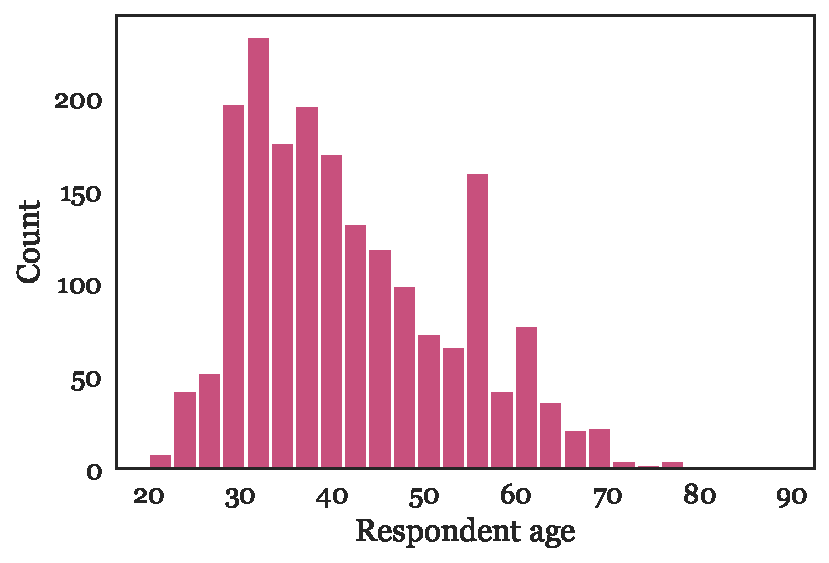
\includegraphics[width=0.33\textwidth,valign=T]{figures/survey/age.pdf}%
% \caption{Age}
% \end{subfigure}
\hfill%
% \begin{subfigure}[t]{0.3\textwidth}
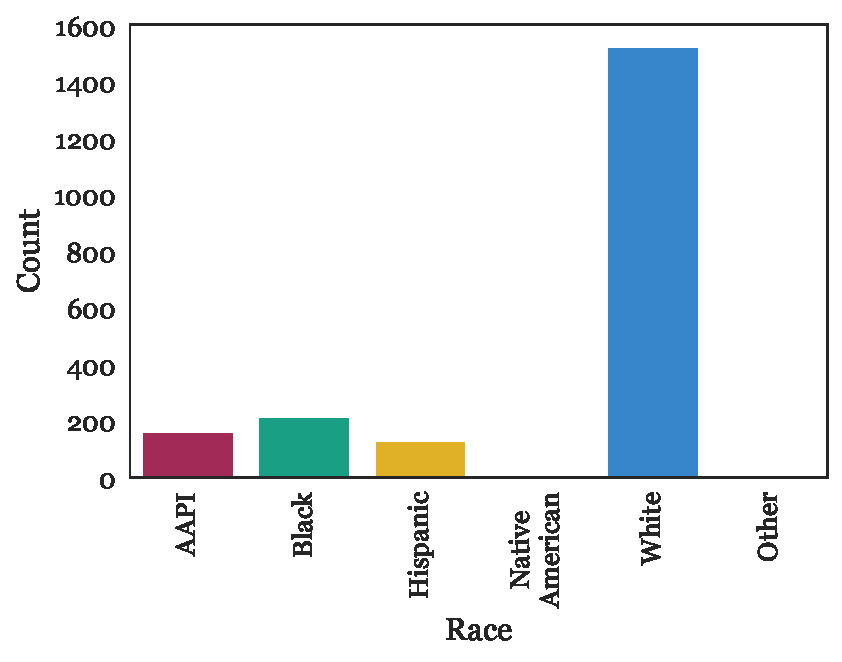
\includegraphics[width=0.33\textwidth,valign=T]{figures/survey/race.pdf}%
% \caption{Race}
% \end{subfigure}
\hfill%
% \begin{subfigure}[t]{0.30.33\textwidth}
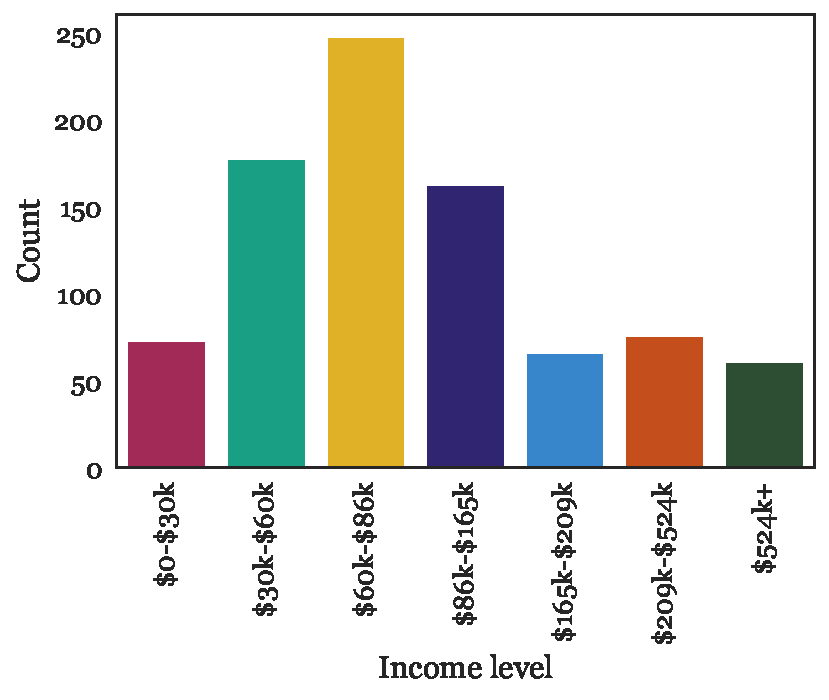
\includegraphics[width=0.33\textwidth,valign=T]{figures/survey/income.pdf}%
% \caption{Income}
% \end{subfigure}
% \\
% \begin{subfigure}[t]{0.3\textwidth}
%     \includegraphics[width=\textwidth]{figures/survey/gender.pdf}
% \caption{Gender}
% \end{subfigure}
% % \hfill
% \begin{subfigure}[t]{0.3\textwidth}
%     \includegraphics[width=\textwidth]{figures/survey/disability.pdf}
% \caption{Disability status}
% \end{subfigure}
\caption{\textbf{Demographic distribution of the participants in our survey.} Respondents appear to have similar demographics to the wider U.S. Mechanical Turk worker population~\cite{pew2016mturkdemog}. Not pictured: respondent gender (43.41\% women, 55.50\% men, 0.83\% non-binary, 0.26\% other), disability status (92.56\% no, 5.74\% yes, 1.70\% prefer not to answer).}
\label{fig:activity_survey_demo}
\end{figure}

\section{Activity Annotation}
\label{as:act_ann}
Obtaining the \bddl definitions for 1,000 activities requires multiple preparatory steps to gather the knowledge needed. This knowledge also becomes part of the~\dataset. The pipeline is outlined in Fig.~\ref{fig:activity_pipeline}. We now detail each annotation other than the survey. Furthermore, quality assessment statistics for these annotations are found in Sec.~\ref{sec:annot_qa}. We see that experienced annotators find our resulting \benchmark knowledge base highly accurate.

\begin{figure}[t]
    \centering
    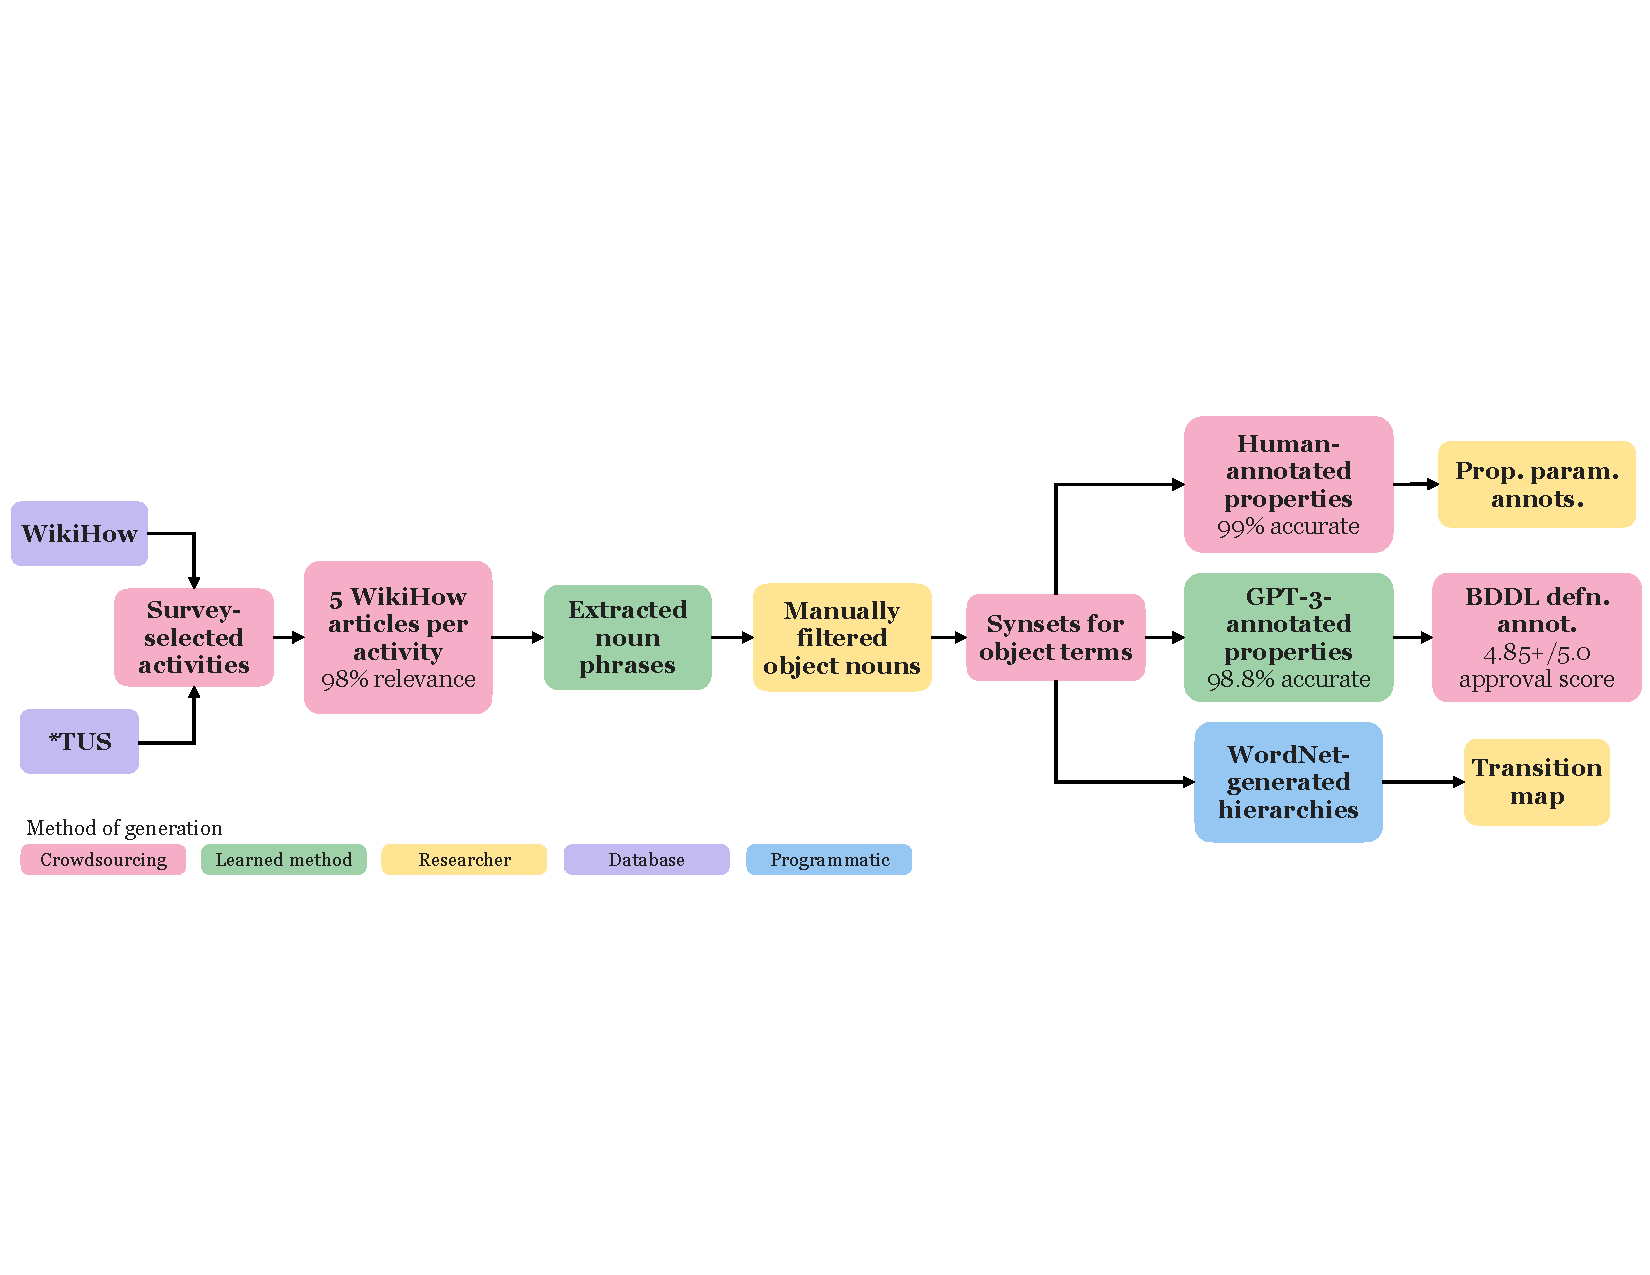
\includegraphics[width=\textwidth]{figures/activities/pipeline.pdf}
    \caption{\textbf{Flow chart of the annotation pipeline:} activity selection, activity article collection, object list extraction, object property and parameter annotation, \bddl annotation.}
    \label{fig:activity_pipeline}
\end{figure}

\paragraph{Obtaining list of objects per activity (WikiHow articles, noun phrase extraction, and manual object filtering):} Our activity definition requires first defining a set of objects and properties that the annotators could use to describe an activity. We would like these domains to be natural and ecological, containing all relevant objects that humans may consider necessary for a task. To obtain such an ecologically plausible object space per activity, we parse WikiHow articles. Since WikiHow is a how-to database with a wide following and community as well as expert- and peer-review, the article texts document objects that are used and acted on in an activity. We therefore asked crowdworkers from the Upwork platform to collect articles; for robustness, we had five articles collected for each activity. We used a chunking model~\cite{akbik2018coling} to extract noun phrases from the article text, then we manually filtered the noun phrases into tangible objects. 

\paragraph{Synsets for object terms and WordNet hierarchy generation:} After obtaining an object space for each activity, we take their union and crowdworkers match each one to a WordNet~\cite{wordnet} synset. This eliminates word-sense ambiguity in the knowledge base and creates a hierarchical structure in the overall object space via the WordNet hierarchy. This process yielded 1,538 total WordNet leaf synsets. Based on various property annotations and needs of the activity set, there are also 1,426 custom synsets for a total of 2,964 leaf synsets.

\paragraph{Property annotations:} Each object that is a leaf-level synset of the WordNet hierarchy is associated with the set of object properties in \benchmark, each of which is fully simulatable in \simulator (full list of properties in Table~\ref{tab:supp_props}). The properties define which predicates can apply to the object - e.g. an object having the \texttt{cookable} property means it can be \texttt{cooked} and \texttt{not cooked}. This association is done task-agnostically because objects/states that are irrelevant or undesirable for a specific activity will still provide important learning signals. All properties that apply to many of the 2,964 leaf synsets and therefore require a large-scale annotation are done by either GPT-3~\cite{gpt3} or crowdworkers. GPT-3 is used for all properties (total of eight) for which the Hamming distance and false-positive rate for a sample compared to a human-annotated ground-truth are both less than 10\%. Human annotation is used for five more properties. The remaining properties are either sensitive to the simulator implementation and are therefore annotated manually, or can be inferred from the other annotations and are determined analytically. 

This annotation is done only for leaf-level synsets, then properties of higher-level synsets are inferred from the leaf-level annotations. This prevents definition unsolveability. In more detail: as shown in Fig.~\ref{fig:activity_pipeline}, the hierarchical structure is applied to the object space. This allows activity definition annotators to refer to them instead of leaf-level synsets; for example, a \texttt{PuttingAwayGroceries} definition can have ``five \texttt{edible\_fruit.n.01}s'' rather than ``two \texttt{apple.n.01}s and three \texttt{banana.n.01}s'', allowing more variation in activity instantiation because far more object models are valid. However, 3-D object models are generally only attached to leaf- or near-leaf-level synsets, meaning that a definition may have a higher-level synset with various predicates attached to it, and at simulation time the object model (associated with one of the synset's descendants) must have those states simulated. A problem might occur when e.g. \texttt{container.n.01} is annotated as \texttt{fillable} and the definition calls for a \texttt{container.n.01} to be \texttt{filled} with a \texttt{liquid}, but the actual model that gets sampled into the simulator to satisfy \texttt{container.n.01} is a cloth bag that doesn't support being \texttt{filled} with a \texttt{liquid}. So to avoid this unsolveability, the properties of any non-leaf synset are exactly the \textit{intersection of all its descendants' properties}.

%\begin{table}[t]
% \centering
% \resizebox{\textwidth}{!}{%
{\scriptsize
\centering
\begin{longtable}{|l|p{.20\textwidth}|p{.25\textwidth}|p{.28\textwidth}|}
        \hline
        \textbf{Object property} & \textbf{Annotation method} & \textbf{Prompt to annotator} & \textbf{Example objects}
        \\\hline
        \texttt{assembleable} & 
            manual &
            N/A & 
             \texttt{desk.n.01},  \texttt{table.n.02}
        \\\hline
        % \texttt{boilable} & 
        %     prog. (all \texttt{liquid}) &
        %     N/A & 
        %      \texttt{champagne.n.01},  \texttt{beef\_broth.n.01}
        % \\\hline
        \texttt{breakable} & 
            human &
            %  Mark if the object can \\be broken into smaller pieces \\by a human dropping it \\on the floor without a tool.\end{tabular} &
            Mark if the object can be broken into smaller pieces by a human dropping it on the floor without a tool.  & 
              \texttt{wine\_bottle.n.01}, \texttt{room\_light.n.01} 
        \\\hline
        % \texttt{cleaningTool} & 
        %     GPT-3 &
        %     %  Is a [object] designed \\to clean things?\end{tabular} & 
        %     Is a [object] designed to clean things? &
        %      \texttt{scrub\_brush.n.01}, \texttt{pipe\_cleaner.n.01}
        % \\\hline
        \texttt{cloth} & 
            manual &
            N/A & 
             \texttt{hammock.n.02}, \texttt{canvas.n.01} 
        \\\hline
        \texttt{coldSource} & 
            GPT-3 &
            Is [object] a source of cold? & 
             \texttt{refrigerator.n.01}, \texttt{ice.n.01}
        \\\hline
        \texttt{cookable} & 
            GPT-3 &
            Can a [object] be cooked? & 
             \texttt{biscuit.n.01},
            \texttt{pizza.n.01}
        \\\hline
        \texttt{deformable} & 
             prog. (all \texttt{softBody}, \texttt{cloth}, \texttt{rope}) &
            N/A & 
              \texttt{tortilla.n.01},  \texttt{clay.n.01} 
        \\\hline
        \texttt{diceable} & 
             prog. (all \texttt{sliceable}'s derivative synsets &
            N/A & 
              \texttt{half\_\_apricot.n.01},  \texttt{half\_\_brisket.n.01} 
        \\\hline
        \texttt{drapeable} & 
             prog. (all \texttt{cloth}, \texttt{rope} &
            N/A & 
              \texttt{dress.n.01},  \texttt{bath\_towel.n.01} 
        \\\hline
        \texttt{fillable} & 
             manual &
            N/A & 
              \texttt{stockpot.n.01},  \texttt{bucket.n.01} 
        \\\hline
        \texttt{fireSource} & 
            GPT-3 &
            %  Is a [object] designed \\to create fire?\end{tabular} & 
            Is a [object] designed to create fire? & 
             \texttt{lighter.n.01}, \texttt{sparkler.n.01} 
        \\\hline
        \texttt{flammable} & 
            human &
            %  Mark if the object can \\catch fire (i.e. burn with \\a flame). For example, \\'wood' and 'gasoline' are \\\textbf{flammable}.\end{tabular}  & 
            Mark if the object can catch fire (i.e. burn with a flame). &
             \texttt{candle.n.01}, \texttt{mail.n.01}
        \\\hline
        \texttt{foldable} & 
             prog. (all \texttt{cloth}, \texttt{softBody}) &
            N/A & 
             \texttt{tortilla.n.01}, \texttt{jean\_jacket.n.01} 
        \\\hline
        \texttt{freezable} & 
             prog. (all \texttt{heatable}) &
            N/A & 
             \texttt{olive\_oil.n.01}, \mbox{\texttt{ginger\_beer.n.01}}
        \\\hline
        \texttt{heatable} & 
            prog. (all rigid bodies) &
            N/A & 
             \texttt{oil.n.01}, \texttt{fish\_knife.n.01} 
        \\\hline
        \texttt{heatSource} & 
            GPT-3 &
            Is a [object] a source of heat? & 
             \texttt{oven.n.01}, \texttt{toaster.n.01} 
        \\\hline
        \texttt{liquid} & 
            GPT-3 &
            Is a [object] a liquid? & 
             \texttt{gasoline.n.01}, \mbox{\texttt{liquid\_soap.n.01}} 
        \\\hline
        \texttt{macroPhysicalSubstance} & 
            manual &
            N/A & 
             \texttt{grated\_cheese.n.01}, \texttt{blueberry.n.02} 
        \\\hline
        \texttt{meltable} & 
            manual &
            N/A & 
             \texttt{cheese.n.01}, \texttt{chocolate.n.02} 
        \\\hline
        \texttt{microPhysicalSubstance} & 
            manual &
            N/A & 
             \texttt{brown\_sugar.n.01}, \texttt{cinnamon.n.03} 
        \\\hline
        \texttt{mixingTool} & 
            manual &
            N/A & 
             \texttt{putty\_knife.n.01}, \texttt{teaspoon.n.02} 
        \\\hline
        \texttt{needsOrientation} & 
            manual &
            N/A & 
             \texttt{cumin\_\_shaker.n.01}, \texttt{salt\_\_shaker.n.01} 
        \\\hline
        \texttt{openable} & 
            human &
            %  Mark if the object is \\designed to be opened.\end{tabular}  & 
            Mark if the object is designed to be opened. &
             \texttt{mixer.n.04}, \texttt{keg.n.01} 
        \\\hline
        \texttt{particleApplier} & 
            manual &
            %  Mark if the object is \\designed to be opened.\end{tabular}  & 
            N/A &
             \texttt{pepper\_mill.n.01}, \texttt{detergent\_\_atomizer.n.01} 
        \\\hline
        \texttt{particleRemover} & 
            GPT-3 &
            %  Mark if the object is \\designed to be opened.\end{tabular}  & 
            Can a [object] absorb liquid? &
             \texttt{scrub\_brush.n.01}, \texttt{broom.n.01} 
        \\\hline
        \texttt{particleSource} & 
            manual (on top of \texttt{particleApplier} &
            %  Mark if the object is \\designed to be opened.\end{tabular}  & 
            N/A &
             \texttt{sink.n.01}
        \\\hline
        \texttt{particleSink} & 
            manual (on top of \texttt{particleRemover} &
            %  Mark if the object is \\designed to be opened.\end{tabular}  & 
            N/A &
             \texttt{sink.n.01}
        \\\hline
        % \texttt{overcookable} & 
        %      prog. (all \texttt{cookable}) &
        %     N/A & 
        %      \texttt{gazpacho.n.01}, \texttt{jam.n.01}
        % \\\hline
        % \texttt{physicalSubstance} & 
        %     manual &
        %     N/A & 
        %      \texttt{flour.n.01}, \texttt{salt.n.02} 
        % \\\hline
        \texttt{rigidBody} & 
            manual &
            N/A & 
             \texttt{tomato.n.01}, \texttt{desk.n.01} 
        \\\hline
        \texttt{rope} & 
            manual &
            N/A & 
             \texttt{ribbon.n.01}, \texttt{fairy\_light.n.01} 
        \\\hline
        \texttt{sliceable} & 
            GPT-3 &
            %  Can a [object] be sliced \\easily by a human \\with a knife?\end{tabular} & 
            Can a [object] be sliced easily by a human with a knife? &
             \texttt{sweet\_corn.n.01}, \mbox{\texttt{sandwich.n.01}} 
        \\\hline
        \texttt{slicingTool} & 
            GPT-3 &
            Can a [object] slice an apple? & 
             \texttt{blade.n.09}, \texttt{razor.n.01}
        \\\hline
        % \texttt{soakable} & 
        %     GPT-3 &
        %     Can a [object] absorb liquid? & 
        %      \texttt{sponge.n.01}, \texttt{tea\_bag.n.01}
        % \\\hline
        \texttt{softBody} & 
            manual &
            N/A & 
             \texttt{dough.n.01}, \texttt{pillow.n.01} 
        \\\hline
        \texttt{substance} & 
             prog. (all \texttt{liquid}, \texttt{vis.Subst.}, \texttt{phys.Subst.}) &
            N/A & 
             \texttt{water.n.06}, \texttt{milk.n.01} 
        \\\hline
        \texttt{toggleable} & 
            human &
            %  The object can be switched \\between a finite number \\of \textit{discrete} states and is \\designed to do so.\end{tabular} & 
            The object can be switched between a finite number of \textit{discrete} states and is designed to do so. &
            %  \texttt{hot\_tub.n.01}, \\ \texttt{light\_bulb.n.01}\end{tabular} \\
            \texttt{hot\_tub.n.01}, \texttt{light\_bulb.n.01} 
        \\\hline
        \texttt{unfoldable} & 
            prog. (all \texttt{foldable}) &
            N/A & 
             \texttt{tissue.n.02}, \texttt{foil.n.01} 
        \\\hline
        \texttt{visualSubstance} & 
            manual &
            N/A & 
             \texttt{coriander.n.02}, \mbox{\texttt{cocoa\_powder.n.01}}
        \\\hline
        \texttt{waterCook} & 
            manual (special case of \texttt{cookable} &
            N/A & 
             \texttt{chickpea.n.01}, \mbox{\texttt{white\_rice.n.01}}
        \\\hline
        % \texttt{waterSource} & 
        %     manual &
        %     N/A & 
        %     \texttt{sink.n.01} 
        % \\\hline
        % \texttt{wetable} & 
        %     prog. (all non-\texttt{substance} &
        %     N/A & 
        %      \texttt{lasagna.n.01}, \texttt{ashtray.n.01}
        % \\\hline
    % \end{tabular}
    \caption{Properties annotated for \benchmark for each object category and included in the \dataset knowledge base}
    \label{tab:supp_props}
\end{longtable}
}
%\end{table}


\paragraph{Property parameter annotations:} \bddl separates objects and object states (i.e. terms and predicates), but simulating realistic ``cooking'' or ``filling'' requires information for object-object property tuples, not just objects or object properties alone. For example, in the real world, an \texttt{apple.n.01} and a \texttt{chicken.n.01} do not become cooked at the same temperature, so simply knowing they are both \texttt{cookable} is insufficient. \dataset therefore includes manual annotation of several property parameters that are (object, object property) specific, such as \texttt{cookTemperature} for all \texttt{cookable} objects. 

Examples of object-property pairs and parameters:
\vspace{-2mm}
\begin{itemize}[leftmargin=2em]
    \item Temperature required for \texttt{cookable} object to go from \texttt{(cooked object) = False} to \texttt{(cooked object) = True}
    \begin{itemize}
        \item \texttt{crab.n.05}: must reach \textbf{63\textdegree C}
        \item \texttt{squash.n.02}: must reach \textbf{58\textdegree C}
         \item \texttt{meatball.n.01}: must reach \textbf{63\textdegree C}
        \item \texttt{chicken\_leg.n.01}: must reach \textbf{74\textdegree C}
    \end{itemize}
    \item Temperature generated by \texttt{heatSource} object. For \texttt{toggleable heatSource}s, this may require \texttt{toggledOn(object) = True}
    \begin{itemize}
        \item \texttt{toaster\_oven.n.01}: generates \textbf{204\textdegree C}
        \item \texttt{ember.n.01}: generates \textbf{1093\textdegree C}
        \item \texttt{hand\_blower.n.01}: generates \textbf{45\textdegree C}
        \item \texttt{coffee\_maker.n.01}: generates \textbf{93\textdegree C}
    \end{itemize}
\end{itemize}



\paragraph{Transition rules:} There are many activities that involve complex chemical and physical processes that are beyond the capability of the state-of-the-art simulation technology. For example, blending different fruits into a smoothie or sanding a rusted surface are extremely difficult to simulate, but the agent actions to complete these tasks are still within reach, e.g. placing the fruits inside a blender. Therefore, in ordet to support these type of activities, we create a set of transition rules that will be used by \simulator to bypass the underlying physics but still produce visually realistic physical transitions, e.g. smoothie particles being generated inside the blender after the blender is turned on.

%simulation, but executing them realistically does not require a deep understanding of those. For example, only certain cleansing agents can clean up grease while many more can clean up the dust. Enforcing this constraint through pure simulation is beyond most state-of-the-art simulators, but for any agent (including a human) that has been given the right materials, the processes are very similar. So, we create a set of transition rules activities including cooking, cleaning, and assembly to make such activities possible and ensure that they require realistic agent actions.

Examples of transition rules: 
\vspace{-2mm}
\begin{itemize}[leftmargin=2em]
    \item Composition and decomposition of objects 
    \begin{itemize}
        \item Transition rule used in \texttt{make a strawberry slushie}
        \begin{itemize}
            \item \textbf{Inputs:} \texttt{strawberry.n.01}, \texttt{ice.n.01}, \texttt{lemon\_juice.n.01}, \texttt{agave.n.01}
            \item \textbf{Transition machine:} \texttt{blender.n.01}
            \item \textbf{Outputs:} \texttt{smoothie.n.01}
        \end{itemize}
        \item Transition rule used in \texttt{make gazpacho}
        \begin{itemize}
            \item \textbf{Inputs:} \texttt{basil.n.03}, \texttt{salt.n.02}, \texttt{black\_pepper.n.02}, \texttt{tomato\_juice.n.01}, \texttt{cucumber.n.02}, \texttt{water.n.06}, \texttt{lemon\_juice.n.01}
            \item \textbf{Transition machine:} \texttt{saucepan.n.01}
            \item \textbf{Outputs:} \texttt{gazpacho.n.01}
        \end{itemize}
    \end{itemize}
    \item Realistic cleaning rules
    \begin{itemize}
    \item Transition rule used in \texttt{CleanTheExteriorOfYourGarage}
    \begin{itemize}
        \item \textbf{Substance covering object:} \texttt{paint.n.01} or \texttt{spray\_paint.n.01}
        \item \textbf{Objects needed to remove:} \texttt{particleRemover} saturated with (\texttt{solvent.n.01} or \texttt{acetone.n.01})
    \end{itemize}
    \item Transition rule used in \texttt{CleanYourRustyGardenTools}
    \begin{itemize}
        \item \textbf{Substance covering object:} \texttt{rust.n.01} or \texttt{patina.n.01} or \texttt{incision.n.01} (simulated as particles but exposed to annotators as unary \texttt{scratched} predicate) or \texttt{tarnish.n.01} (simulated as particles but exposed to annotators as unary \texttt{tarnished} predicate)
        \item \textbf{Objects needed to remove:} \texttt{emery\_paper.n.01} or \texttt{whetstone.n.01}
    \end{itemize}
    \end{itemize}
\end{itemize}

\paragraph{Activity definitions in \bddl:} Finally, the object spaces and the relevant properties and predicates they enable are offered to lay annotators to generate \bddl definitions. Annotators build activity definitions using an annotation interface that includes a visual version of \bddl~\cite{srivastava2021behavior} (details on new features in \bddl are in  Sec.~\ref{sec:bddl}). The annotation interface enforces the requirements needed to make definitions logically solvable and well-formed. We collect one definition per activity for a total of 1,000 \bddl activity definitions.

Listings~\ref{lst:bddl3},~\ref{lst:bddl4}, and~\ref{lst:bddl5} show examples of \benchmark activity definitions, while Listing~\ref{lst:bddl1} and~\ref{lst:bddl2} show examples of \oldbenchmark definitions. We see that while the numbers of objects and literals are similar, speaking to the fact that both benchmarks have reached similar scale and detail for the activities they have, \benchmark has far larger and more detailed activity distribution. The \texttt{BakingSugarCookies} activity involves transition rules that turn ingredients in \texttt{:init} to scones in \texttt{:goal}, a process that will require the listed mixer and oven in \simulator. By contrast, cooking in \oldbenchmark was limited to single objects transitioning from \texttt{not cooked} to \texttt{cooked}; other benchmarks are similar or lack cooking entirely. \texttt{CleanYourLaundryRoom} involves specific cleansing agents to clean mold, whereas \oldbenchmark cleaning tasks only had two types of ``dirtiness'' (\texttt{stained} and \texttt{dusty}) and the only rule was to use water in the case of \texttt{stained}. \texttt{CleanTheBottomOfAnIron} also shows rust-specific cleaning (requiring emery paper).

\subsection{Quality assessment of \benchmark annotations}
\label{sec:annot_qa}
% TODO 

\begin{table}[h]
    \centering
     \resizebox{\textwidth}{!}{  
    \begin{tabular}{|c|c|c|c|c|}
        \hline
        & Article Collection & Object Extraction & Human Properties & GPT-3 / Machine Properties \\ %& Parameter Annotation &  Activity Definition \\
         \hline
        Accuracy (Approval Rate)  & 0.974 & 0.968 & 0.990 & 0.988 \\ % & & \\
        \hline
        F1-score & 0.984 & 0.990 & 0.912 & 0.930 \\ % & & \\
        \hline
        False Discovery Rate & 0.026 & 0.032 & 0.031 & 0.029 \\ % & & \\
        \hline
        False Positive Rate & N/A & N/A & 0.002 & 0.003 \\ % & & \\
        \hline
    \end{tabular}}
    \caption{Quality check results for object and object property annotations: for each stage in the annotation pipeline, report human verification results. The F1-score is $\frac{2}{\texttt{precision}^{-1} + \texttt{recall}^{-1}}$. The False Discovery Rate is FDR = FP/(TP+FP) and the False Positive Rate FPR = FP/(TN+FP). The high accuracy and F1-scores and low FDRs and FPRs show that our annotation results are of high quality. }
    \label{tab:activity_qc}
\end{table}

\begin{table}[h]
    \centering
     \resizebox{10cm}{!}{  
    \begin{tabular}{|c|c|c|c|c|}
    \hline
    %    \hline
    & \multicolumn{4}{c|}{Activity Definition} \\
        %\cline{1-8}
        \hline
        & Question 1 & Question 2 & Question 3 & Question 4\\ %& Parameter Annotation &  Activity Definition \\
         \hline
        Average Rating  & 4.875 & 4.942 & 4.967 & 4.975 \\ % & & \\
        \hline
        Standard Deviation & 0.331 & 0.234 & 0.364 & 0.156 \\ % & & \\
    \hline
    \end{tabular}}
    \caption{Quality check results for activity definitions. Q1: Are the objects listed relevant to the definition of the task?, Q2: Do the initial placements/locations of objects make sense?, Q3: Are the actions to perform (“goals”) relevant to the definition of the activity?, Q4: Is this definition reasonable?\\ 
    Each activity definition was evaluated on a scale of 1-5 for each of the questions, and the average score and standard deviation are presented. The increased granularity still reflects the high quality of our results.}
    \label{tab:bddl_def_qc}
\end{table}

Our quality control investigation shows us that all labeling done by crowdworkers and GPT-3 is of the highest quality. Five crowdworkers with an extensive background in data labeling for large machine learning projects, coding, or data verification affirmed the results from earlier crowdworkers. The accuracies for all the labeling tasks were all above 96\%, the F1 scores were above 91\% and the false positive and false discovery rates were between 2-3\% as shown in Table~\ref{tab:activity_qc}. We noticed that the Synset Verification is a bit lower in accuracy than the other labeling tasks. This may be due to subtleties in acceptable synset definitions: for example, a ''reasonably narrow hypernym'' of a word not found in WordNet~\cite{wordnet} is acceptable, such as a "dispenser" for a "soap dispenser", but there may be gray areas regarding what is considered "reasonably narrow" (e.g. would a "hand tool" be reasonable as a replacement for a "soap dispenser"?)

The activity definition process was evaluated with more granularity using a Likert scale and an array of questions. We found that the response values had consistently high averages (very close to the maximum score of 5) and low standard deviations as shown in Table~\ref{tab:activity_qc}. We also found no significant discrepancy for activity definition scores across topics (e.g. tasks related to "cleaning"), showing that the \bddl definitions were rated uniformly across the span of activity categories.

\section{New \bddl features}
\label{sec:bddl}

\benchmark uses an expanded version of the~\bddl used in \oldbenchmark~\cite{srivastava2021behavior}, in order to support the new set of diverse activities. There are three new features here: 1) representation of substances, 2) three-valued predicates, and 3) composition and decomposition of objects. %, and 4) variable-arity predicates. We now detail the need for each of these, why the~\bddl from \oldbenchmark cannot support them, and the design in this version of~\bddl.

\paragraph{Representation of substances:} \benchmark introduces \textit{substances}, objects that are arbitrarily subdivideable and do not obey clear instance boundaries such as \texttt{water.n.06} or \texttt{flour.n.01}. The lack of instance boundaries is difficult with traditional PDDL/\bddl: for example, if there are two bottles of orange juice where the juice inside one is called \texttt{orange\_juice.n.01\_1} and the juice inside the other is called \texttt{orange\_juice.n.01\_2}, any mixing of the particles makes it near-impossible for the agent to satisfy a \texttt{:goal} condition pertaining to an instance. Even with quantification, a condition like \texttt{exists (orange\_juice.n.01) (filled orange\_juice.n.01 glass.n.01\_3)} is still unfair: if the agent mixes particles from the two different \texttt{orange\_juice} instances such that together they \texttt{filled glass.n.01\_3} but neither instance alone has enough particles in \texttt{glass.n.01\_3} to fill it, the \texttt{:goal} will not be met.

We simply enforce that there is up to one instance of any \texttt{substance} in a definition. The annotator can still control quantity by spawning it in as many containers as desired. Unlike labeling every particle separately, this maintains a compact representation. This does not allow for some of the substances to be different from some (e.g. some of the orange juice is cold and some is hot), but we consider this an acceptable limitation.

Furthermore, particle-based objects can be computationally expensive to simulate. When an annotator uses \texttt{orange\_juice.n.01} only as a container of orange juice and not actually the particles (e.g. in a \texttt{PuttingAwayGroceries} activity), this becomes a waste of computational resources. Therefore, we introduce a custom container synset for every substance that has the same properties and WordNet hierarchy structure as \texttt{bottle.n.01} and instruct annotators to use it if all they want is the container.

\paragraph{Three-valued predicates:} A common issue in \oldbenchmark activities is that success on predicates involving naturally continuous-valued quantities is sudden and arbitrary: cracking a window a little bit suddenly changes it from \texttt{not open} to \texttt{open}, and the activity from undone to done – even though the window is not a typical human conception of ``open’’. PDDL 2.1~\cite{fox2003pddl21} has numerical fluents and derived predicates, which offer continuous states. However, this granularity may not be crucial to the high-level activities in \benchmark, and the concept is also difficult to communicate to lay annotators.

We therefore treat certain predicates as three-valued by having two Boolean predicates where the negations are the same, such as \texttt{filled} and \texttt{empty} (rather than just \texttt{not filled}). The annotators still see one Boolean predicate, in this case \texttt{filled}, and negate it to say the opposite, but we assume that when they negate, they mean something decisively empty. This is a strong assumption but generally safe as people tend not to add expressions that seem like common sense. Wherever we see the predicate negated in the definition, we switch it out with the other predicate. This applies to \texttt{filled}/\texttt{empty}, \texttt{open}/\texttt{closed}, and \texttt{folded}/\texttt{unfolded}.

To ensure that the definition is logically the same after the switch, the underlying~\bddl implementation converts the definition using De Morgan’s Law such that all negations are only applied to atomic formulae before the switch occurs.

% The only logical pitfall is that the switch does not work for all expressions: \texttt{not (exists (sweater.n.01) (folded sweater.n.01))} is not the same as \texttt{(exists (sweater.n.01) (unfolded sweater.n.01))}
% \texttt{exists (?sweater.n.01) (not (folded sweater.n.01))} is not the same as \texttt{exists (?sweater.n.01) (unfolded sweater.n.01)} – in the first expression, there could be a sweater that is in between \texttt{unfolded} and \texttt{folded}. Instead,  

\paragraph{Composition and decomposition of objects:} In standard PDDL/~\bddl, the objects in \texttt{:objects} are assumed to persist throughout the activity. There is no concept of creating a new object that did not appear in the \texttt{:init} or explicitly destroying an object. 

To enable our transition rules that involve turning some objects into others, we require a representation that will provide the desired information unambiguously. The \texttt{:objects} section cannot be inferred simply from a \texttt{:goal} that has new objects in it, because \texttt{:goal} is not exhaustive. We therefore introduce the \texttt{future} predicate, used in \texttt{:init} on all objects that do not appear in the scene when the agent enters, but must be present for the \texttt{:goal} to be satisfied. All objects in \texttt{future} predicates appear in \texttt{:objects} and they cannot appear in any other literals in \texttt{:init}. This approach takes inspiration from~\cite{wichlacz2019ghost}, which updates a reference to an object (e.g. a wall) as it keeps changing form as more sub-objects (e.g. blocks) are added to it.

% \paragraph{Variable-arity predicates:} Certain predicates can take various numbers of objects while indicating the same underlying concept. For example, in \benchmark, the \texttt{mixed} predicate can take any number of objects: the expressions \texttt{(mixed apple.n.01\_1 apple.n.01\_2 peach.n.03\_1)} and \texttt{(mixed apple.n.01\_1 apple.n.01\_2 peach.n.03\_1 banana.n.01\_1)} give different numbers of objects to \texttt{mixed}, but mean the same thing and are checked the same way in~\simulator. 

% Logic predicates are fixed-arity by default, but work exists to expand to variable-arity predicates~\cite{oliver2004multigrade}. PDDL uses this assumption to specify predicates in its domain that can be used with PDDL actions to create plans. However, because~\bddl is used for benchmarking, it is process-agnostic and does not assume any planning method~\cite{srivastava2021behavior}. Therefore, a domain file does not have any effect in~\bddl, so a variable-arity predicate can be specified (rather than potentially infinite fixed-arity versions) to maintain compactness. This requires no structural changes to~\bddl.



%\begin{longtable}{|p{0.3\textwidth}|p{0.3\textwidth}|p{0.3\textwidth}|}
\hline 1. washing floor & 2. cleaning bathrooms & 3. clean your house after a wild party & 4. cleaning floors \\
\hline 
 5. mopping floors & 6. clean a shower & 7. cleaning toilet & 8. cleaning bathtub \\
\hline 
 9. clean grease & 10. scrubbing bathroom floor & 11. cleaning oven & 12. cleaning stove \\
\hline 
 13. shoveling snow & 14. washing outside windows & 15. clean walls & 16. clean up water damage \\
\hline 
 17. washing dishes & 18. vacuuming floors & 19. picking up trash & 20. clean carpets \\
\hline 
 21. emptying trash cans & 22. cleaning pavement & 23. washing plates & 24. washing outside walls \\
\hline 
 25. cleaning windows & 26. sweeping floors & 27. clean the outside of a house & 28. taking trash outside \\
\hline 
 29. clean a couch & 30. washing pots and pans & 31. remove hard water spots & 32. cleaning barbecue grill \\
\hline 
 33. clean a stainless steel dishwasher & 34. sweeping porch & 35. raking leaves & 36. clean cement \\
\hline 
 37. putting dishes away after cleaning & 38. clean your kitty litter box & 39. washing windows & 40. mopping the kitchen floor \\
\hline 
 41. clean outdoor tiles & 42. remove spots from linen & 43. cleaning microwave oven & 44. clean wood siding \\
\hline 
 45. clean a coffee maker & 46. picking up litter & 47. cleaning up after a meal & 48. clean a drain \\
\hline 
 49. clean a sofa & 50. cleaning vehicles & 51. polish wood floors & 52. clean up after a dinner party \\
\hline 
 53. remove ice from gutters & 54. cleaning carpets & 55. sweeping outside entrance & 56. clean mirrors \\
\hline 
 57. clean a broiler pan & 58. vacuuming vehicles & 59. disposing of lawn clippings & 60. cleaning the pool \\
\hline 
 61. unloading shopping from car & 62. waxing cars or other vehicles & 63. clean a grill pan & 64. mowing the lawn \\
\hline 
 65. cleaning up refrigerator & 66. clean your rusty garden tools & 67. removing ice from walkways & 68. cleaning bedroom \\
\hline 
 69. cleaning debris out of car & 70. sweeping garage & 71. wash towels & 72. washing walls \\
\hline 
 73. washing cars or other vehicles & 74. moving stuff to storage & 75. disposing of trash for adult & 76. assembling furniture \\
\hline 
 77. clearing the table after dinner & 78. clean your laundry room & 79. cleaning up after an event & 80. clean an air filter \\
\hline 
 81. tidying bathroom & 82. cleaning up plates and food & 83. installing carpet & 84. cleaning a car \\
\hline 
 85. cleaning the hot tub & 86. moving boxes to storage & 87. clean up gasoline & 88. clean decking \\
\hline 
 89. clean the exterior of your garage & 90. doing laundry & 91. dusting rugs & 92. clean cups \\
\hline 
 93. clean a mattress & 94. shampooing carpet & 95. clean sheets & 96. cleaning up branches and twigs \\
\hline 
 97. waxing floors & 98. clean kitchen appliances & 99. hoe weeds & 100. storing the groceries \\
\hline 
 101. changing sheets & 102. clean rubber bathmats & 103. clean a chicken coop & 104. scraping snow off vehicle \\
\hline 
 105. cleaning patio furniture & 106. cleaning the yard & 107. folding clean laundry & 108. cleaning driveway \\
\hline 
 109. cleaning kitchen cupboard & 110. folding sheets & 111. clean plastic containers & 112. clean a rug \\
\hline 
 113. clean a vacuum & 114. cleaning cupboards & 115. clean your baseboard radiators & 116. clean stainless steel sinks \\
\hline 
 117. clean a glass windshield & 118. clean household cleaning tools & 119. cleaning garden tools & 120. water your lawn efficiently \\
\hline 
 121. ironing clothes & 122. cleaning fan & 123. chop an onion & 124. clean a toaster oven \\
\hline 
 125. disinfect laundry & 126. cleaning up the kitchen only & 127. chopping wood & 128. painting house exterior \\
\hline 
 129. de-clutter your garage & 130. washing utensils & 131. cleaning garage & 132. laying tile floors \\
\hline 
 133. washing fabrics & 134. washing curtains & 135. folding clothes & 136. unpacking moving van \\
\hline 
 137. clean a kitchen sink & 138. shoveling coal & 139. cleaning freezer & 140. putting away yard equipment \\
\hline 
 141. cleaning pet bed & 142. clean a air conditioner & 143. clean out a guinea pigs hutch & 144. clean up broken glass \\
\hline 
 145. clean a rice cooker & 146. polisha car & 147. clean your cleaning supplies & 148. clean a fish \\
\hline 
 149. bringing laundry & 150. applying pesticides & 151. sweeping patio & 152. cleaning shed \\
\hline 
 153. cleaning closet & 154. cleaning table after clearing & 155. putting away Christmas decorations & 156. cleaning parks \\
\hline 
 157. clean a fence & 158. polishing silver & 159. hanging blinds & 160. doing housework for adult \\
\hline 
 161. cleaning the pond & 162. re-shelving library books & 163. clean couch pillows & 164. putting clean laundry away \\
\hline 
 165. rinsing dishes & 166. sweeping steps & 167. polishing furniture & 168. unloading the car \\
\hline 
 169. putting pesticides on lawn & 170. clean an espresso machine & 171. cleaning around pool in garden & 172. clean the interior of your car \\
\hline 
 173. bringing paper to recycling & 174. clean stucco & 175. spraying for bugs & 176. cleaning lawnmowers \\
\hline 
 177. cleaning tools and equipment & 178. laying wood floors & 179. clean a keyboard & 180. putting laundry in drawer \\
\hline 
 181. treating stains & 182. washing bowls & 183. clean a popcorn machine & 184. clean a dirty tent \\
\hline 
 185. clean a baking stone & 186. organizing boxes in garage & 187. clean up spilled egg & 188. changing dog's water \\
\hline 
 189. cleaning boat & 190. clean reusable shopping bags & 191. clean wood doors & 192. dispose of a pizza box \\
\hline 
 193. drying dishes & 194. clean a faucet & 195. prepare a raised bed garden & 196. loading the dishwasher \\
\hline 
 197. clean brass casings & 198. removing lint from dryer & 199. bringing glass to recycling & 200. making the bed \\
\hline 
 201. clean a patio & 202. laying paving stones & 203. clean the bottom of an iron & 204. putting up wallpaper \\
\hline 
 205. fertilize a lawn & 206. cleaning restaurant table & 207. clean an electric razor & 208. lay sod \\
\hline 
 209. clean a hot water dispenser & 210. clean baking sheets & 211. clean a sauna & 212. clean vinyl shutters \\
\hline 
 213. clean a kitchen table & 214. collecting dishes from restaurant tables & 215. delivering groceries to doorstep & 216. clean flip flops \\
\hline 
 217. taking clothes off of the drying rack & 218. cleaning stuff out of car & 219. installing a fence & 220. store firewood \\
\hline 
 221. wash jeans & 222. clean a light bulb & 223. clean rubber & 224. make coffee \\
\hline 
 225. chopping vegetables & 226. fixing broken table & 227. cleaning camper/RV & 228. organise a linen closet \\
\hline 
 229. wash duvets & 230. stock grocery shelves & 231. clean and disinfect ice trays & 232. clean a hamper \\
\hline 
 233. make cabinet doors & 234. replacing screens & 235. tidying living room & 236. clean a box fan \\
\hline 
 237. clean potatoes & 238. carrying in groceries & 239. cleaning garden path & 240. polish copper \\
\hline 
 241. mulching & 242. hanging up curtains & 243. clean a birdcage & 244. de-ice a car \\
\hline 
 245. polishing shoes & 246. loading shopping into car & 247. clearing table after breakfast & 248. remove scorch marks \\
\hline 
 249. cleaning sneakers & 250. hand washing clothing & 251. clearing table after dinner & 252. washing vegetables \\
\hline 
 253. adding chemicals to lawn & 254. dust houseplants & 255. watering outdoor flowers & 256. turning sprinkler off \\
\hline 
 257. dispose of glass & 258. clean a felt pool table top & 259. putting away toys & 260. painting porch \\
\hline 
 261. spraying fruit trees & 262. putting shopping away & 263. cleaning fishing gear & 264. brushing lint off clothing \\
\hline 
 265. clean a blender & 266. stacking wood & 267. loading the car & 268. sanding wood furniture \\
\hline 
 269. clean a toaster & 270. adding chemicals to pool & 271. remove sod & 272. bringing in wood \\
\hline 
 273. clean a sponge & 274. cleaning shoes & 275. clean a piano & 276. store firewood outdoors \\
\hline 
 277. clean a small pet cage & 278. clean brooms & 279. composting waste & 280. getting package from post office \\
\hline 
 281. picking up toys & 282. fertilizing garden & 283. clean quarters & 284. clean a pickup truck \\
\hline 
 285. picking up baggage & 286. recycling office papers & 287. collecting dishes from around house & 288. clean brass \\
\hline 
 289. disinfect nail clippers & 290. putting away Halloween decorations & 291. clearing table after supper & 292. installing appliances \\
\hline 
 293. sorting bottles, cans, and paper & 294. clean a company office & 295. clean a raincoat & 296. lube a bicycle chain \\
\hline 
 297. dispose of paper & 298. clean place mats & 299. clean leather sandals & 300. unloading shopping items \\
\hline 
 301. putting on license plates & 302. fertilize plants & 303. clean cup holders & 304. wash dog toys \\
\hline 
 305. turning sprinkler on & 306. taking clothes out of the dryer & 307. changing bulbs & 308. tidy your garden \\
\hline 
 309. clean wood pallets & 310. clean your electronics & 311. unpacking car for trip & 312. locking every door \\
\hline 
 313. clearing table after snacks & 314. haul a motorcycle & 315. clean a garden sprayer & 316. clean a whiteboard \\
\hline 
 317. recycling newspapers & 318. fill a punching bag & 319. packing moving van & 320. picking up take-out food \\
\hline 
 321. defrosting freezer & 322. line kitchen shelves & 323. clean black rims & 324. recycling glass bottles \\
\hline 
 325. unloading groceries & 326. putting protective cover on vehicle & 327. putting up shelves & 328. sorting laundry \\
\hline 
 329. clean a backpack & 330. carrying out garden furniture & 331. hanging clothes & 332. cleaning glasses off bar \\
\hline 
 333. clean clear plastic & 334. ironing bedsheets & 335. prepare your garden for winter & 336. chlorinating the pool \\
\hline 
 337. hanging clothes on clothesline & 338. putting clothes into closet & 339. putting up Christmas lights outside & 340. clean soot from glass lanterns \\
\hline 
 341. clean a golf club & 342. watering outdoor plants & 343. putting leftovers away & 344. returning consumer goods \\
\hline 
 345. fixing mailbox & 346. hooking up trailer to car & 347. clean a computer monitor & 348. clean pottery \\
\hline 
 349. putting towels in bathroom & 350. clean a dirty baseball & 351. tidying bedroom & 352. repairs to furniture \\
\hline 
 353. cook chicken and rice & 354. clean shrimp & 355. bag groceries & 356. putting dirty dishes in sink \\
\hline 
 357. clean an electric kettle & 358. clean piano keys & 359. cooking food for adult & 360. clean a pizza stone \\
\hline 
 361. collecting wood & 362. putting up Christmas decorations outside & 363. clean gas logs & 364. clean garden gloves \\
\hline 
 365. clean a flat iron & 366. picking up clothes & 367. clean copper wire & 368. remove a broken light bulb \\
\hline 
 369. unpacking recreational vehicle for trip & 370. throwing out used napkins & 371. making photocopies & 372. stripping furniture \\
\hline 
 373. bringing in mail & 374. wash a motorcycle & 375. planting trees & 376. clean clams \\
\hline 
 377. sorting clothing & 378. carrying water & 379. cleaning high chair & 380. turning out all lights before sleep \\
\hline 
 381. cleaning rainboots & 382. covering boat & 383. spray stucco & 384. make pizza \\
\hline 
 385. clean a LED screen & 386. changing light bulbs & 387. brewing coffee & 388. wash your bike \\
\hline 
 389. make pastry & 390. set up a coffee station in your kitchen & 391. putting away tools & 392. clean a gravestone \\
\hline 
 393. clearing table after coffee & 394. polish pewter & 395. thawing frozen food & 396. make ice \\
\hline 
 397. setting mousetraps & 398. clean vases & 399. clean quartz & 400. dispose of batteries \\
\hline 
 401. collect misplaced items & 402. locking every window & 403. cook pasta & 404. clean vans \\
\hline 
 405. can vegetables & 406. ironing curtains & 407. bringing in kindling & 408. putting away cleaning supplies \\
\hline 
 409. folding piece of cloth & 410. installing smoke detectors & 411. clean a quilt & 412. sorting newspapers for recycling \\
\hline 
 413. picking up prescriptions & 414. taking clothes out of washer & 415. putting clothes in storage & 416. reheat frozen or chilled food \\
\hline 
 417. sorting clothes & 418. fixing broken chair & 419. clean an office chair & 420. wash an infant car seat \\
\hline 
 421. hanging up bedsheets & 422. hang icicle lights & 423. organizing items for yard sale & 424. staining wood furniture \\
\hline 
 425. clean a suitcase & 426. returning videotapes to store & 427. putting up outdoor holiday decorations & 428. clean a beer keg \\
\hline 
 429. setting up bedroom for guest & 430. prepare make ahead breakfast bowls & 431. clean a knife block & 432. decorating outside for holidays \\
\hline 
 433. wash baby bottles & 434. sending packages & 435. clean a saxophone & 436. setting the table \\
\hline 
 437. laying restaurant table for dinner & 438. taking clothes off the line & 439. packing boxes for household move or trip & 440. fold towels \\
\hline 
 441. putting in a hot tub & 442. hanging shades & 443. clean a trumpet & 444. clean green beans \\
\hline 
 445. clean a razor blade & 446. clean a bicycle chain & 447. cleaning cups in living room & 448. clean a knife \\
\hline 
 449. clean silver coins & 450. make edible chocolate chip cookie dough & 451. wash lettuce & 452. make instant coffee \\
\hline 
 453. cook fish & 454. clean leather boots & 455. hanging outdoor lights & 456. clean synthetic hiking gear \\
\hline 
 457. organizing file cabinet & 458. unpacking suitcase & 459. clean a lobster & 460. clean sunglasses \\
\hline 
 461. clean a sauna suit & 462. make toast & 463. clean a flat panel monitor & 464. iron curtains \\
\hline 
 465. packing grocery bags into car & 466. packing books into car & 467. make muffins & 468. make pizza dough \\
\hline 
 469. installing a trailer hitch & 470. clean a sieve & 471. make brownies & 472. cook bacon \\
\hline 
 473. prepare baking pans & 474. putting out clean towels & 475. cleaning computer & 476. organizing office documents \\
\hline 
 477. watering indoor flowers & 478. setting up garden furniture & 479. store batteries & 480. clean a wood pipe \\
\hline 
 481. packing cleaning suppies into car & 482. watering houseplants & 483. set up a buffet & 484. planting plants \\
\hline 
 485. wash a bra & 486. set a dinner table & 487. dispose of fireworks & 488. clean oysters \\
\hline 
 489. putting out dog food & 490. clean a mousepad & 491. installing alarms & 492. cook onions \\
\hline 
 493. clean a teddy bear & 494. clean white wall tires & 495. tidying up wardrobe & 496. gathering nuts \\
\hline 
 497. clean a crab & 498. clearing food from table into fridge & 499. putting away purchased clothes & 500. clean copper mugs \\
\hline 
 501. cleaning kitchen knives & 502. clean tennis balls & 503. make chicken fajitas & 504. make soup \\
\hline 
 505. clean a hat & 506. store winter coats & 507. cleaning skis & 508. clean wine glasses \\
\hline 
 509. hanging pictures & 510. store christmas lights & 511. setting up for an event & 512. clean a bowling ball \\
\hline 
 513. wash a wool coat & 514. wash delicates in the laundry & 515. bringing newspaper in & 516. make dinner rolls \\
\hline 
 517. wash goalkeeper gloves & 518. cleaning out drawers & 519. make a small vegetable garden & 520. cooking breakfast \\
\hline 
 521. emptying ashtray & 522. making coffee & 523. make lemon stain remover & 524. treating clothes \\
\hline 
 525. boxing food after dinner & 526. preserving food & 527. clean a tie & 528. clean dog collars \\
\hline 
 529. cook chicken & 530. packing lunches & 531. remove a wall mirror & 532. filling the bird feeder \\
\hline 
 533. clean an iron & 534. putting in a pool & 535. packing fishing gear into car & 536. store rugs \\
\hline 
 537. clean your pencil case & 538. buy pet food for less & 539. slicing vegetables & 540. clean vintage stereo equipment \\
\hline 
 541. cook noodles & 542. thaw frozen fish & 543. make a blended iced cappuccino & 544. buying postage stamps \\
\hline 
 545. store an uncooked turkey & 546. planting flowers & 547. clean nickel & 548. clean fur \\
\hline 
 549. clean tweed & 550. clean batting gloves & 551. boil water & 552. clean a leather belt \\
\hline 
 553. setup a fish tank & 554. prepare a breakfast bar & 555. polish gold & 556. clean white marble \\
\hline 
 557. can syrup & 558. canning food & 559. make cookies & 560. wash fruit and vegetables \\
\hline 
 561. heating soup & 562. putting food in fridge & 563. clean a purse & 564. make batter \\
\hline 
 565. iron a tie & 566. defrost meat & 567. setup a trampoline & 568. clean dentures \\
\hline 
 569. set up two computer monitors & 570. mailing letters & 571. cooking dinner & 572. cooking lunch \\
\hline 
 573. clean prawns & 574. make cake mix & 575. freeze meat & 576. clean a turkey \\
\hline 
 577. rearrange your room & 578. make pizza sauce & 579. putting away games & 580. make nachos \\
\hline 
 581. make a bake sale stand stall & 582. clean paper lampshades & 583. store coffee beans or ground coffee & 584. make popsicles \\
\hline 
 585. polish cymbals & 586. buy boxes for packing & 587. can beans & 588. clean mushrooms \\
\hline 
 589. collecting aluminum cans & 590. puttiing away bicycles & 591. sorting items for garage sale & 592. treating spot \\
\hline 
 593. sorting potatoes & 594. boxing books up for storage & 595. prepare a hanging basket & 596. clean cork mats \\
\hline 
 597. cook rice & 598. clean a pumpkin & 599. hang a dartboard & 600. clean scallops \\
\hline 
 601. storing food & 602. fill a hot water bottle & 603. clean up your desk & 604. heating food up \\
\hline 
 605. fold a cloth napkin & 606. clean jade & 607. clean marker off a doll & 608. grill vegetables \\
\hline 
 609. make fried rice & 610. make an iced espresso & 611. collecting mail from the letterbox & 612. roast vegetables \\
\hline 
 613. clean a watch & 614. make lemon or lime water & 615. store produce & 616. buying cleaning supplies \\
\hline 
 617. clean boxing gloves & 618. praeparing lunch box & 619. planting vegetables & 620. setup a garden party \\
\hline 
 621. clean gourds & 622. make granola & 623. picking vegetables in garden & 624. cook vegetables \\
\hline 
 625. make strawberries and cream & 626. taking down curtains & 627. putting out cat food & 628. organizing volunteer materials \\
\hline 
 629. picking up books at library & 630. clean suede gloves & 631. cook sweet potatoes & 632. wash a leotard \\
\hline 
 633. wash a baseball cap & 634. clean wooden blocks & 635. putting on tags (car) & 636. make cream from milk \\
\hline 
 637. can fruit & 638. prepare and cook prawns & 639. clean your goal keeper gloves & 640. adding fabric softener \\
\hline 
 641. make a cappuccino & 642. sorting household items & 643. clean strawberries & 644. cook ramen noodles \\
\hline 
 645. prepare a filling breakfast & 646. cool cakes & 647. cleaning mushrooms & 648. clean snow peas \\
\hline 
 649. buy home use medical supplies & 650. taking fish out of freezer & 651. making tea & 652. make blueberry mousse \\
\hline 
 653. getting organized for work & 654. making a meal & 655. cook ground beef & 656. preserving vegetables \\
\hline 
 657. make waffles & 658. putting wood in fireplace & 659. putting tablecloth on table & 660. hang a bike on the wall \\
\hline 
 661. make a sugar and coffee scrub & 662. setting up room for a movie & 663. clean snap peas & 664. make a cheese pastry \\
\hline 
 665. make a mojito & 666. wash a backpack & 667. store baby clothes & 668. clean a longboard \\
\hline 
 669. make fish and chips & 670. serving hors d oeuvres & 671. unpacking hobby equipment & 672. cook asparagus \\
\hline 
 673. clean eggs & 674. cook mussels & 675. buy mulch & 676. make iced chocolate \\
\hline 
 677. putting shoes on rack & 678. clean jewels & 679. make applesauce & 680. setting up room for games \\
\hline 
 681. cold brew coffee & 682. make a strawberry slushie & 683. clean a candle jar & 684. cook corn \\
\hline 
 685. rearranging furniture & 686. make a clothes line & 687. cook a brisket & 688. make stew \\
\hline 
 689. turning off the hot tub & 690. baking cookies for the PTA bake sale & 691. cook oysters & 692. grill burgers \\
\hline 
 693. make bagels & 694. throwing away leftovers & 695. drying table & 696. packing hiking equipment into car \\
\hline 
 697. organizing art supplies & 698. buy dog food & 699. make cake filling & 700. installing a printer \\
\hline 
 701. sorting groceries & 702. clean a trombone & 703. packing sports equipment into car & 704. packing art supplies into car \\
\hline 
 705. packing recreational vehicle for trip & 706. putting up posters & 707. cook green beans & 708. make pasta sauce \\
\hline 
 709. prepare your garden for a cat & 710. adding chemicals to hot tub & 711. cook lamb & 712. packing meal for delivery \\
\hline 
 713. turning on radio & 714. make seafood stew & 715. hanging address numbers & 716. glaze a ham \\
\hline 
 717. buying groceries for a feast & 718. collecting berries & 719. cook potatoes & 720. clean baby toys \\
\hline 
 721. make macaroni and cheese & 722. clean geodes & 723. prepare wine and cheese & 724. make a tropical breakfast \\
\hline 
 725. organizing school stuff & 726. rearranging kitchen furniture & 727. attach a camera to a tripod & 728. setting table for coffee \\
\hline 
 729. toast buns & 730. make meatloaf & 731. make tacos & 732. buy rechargeable batteries \\
\hline 
 733. clean mussels & 734. distributing groceries at food bank & 735. filling salt & 736. make baked pears \\
\hline 
 737. installing a scanner & 738. hanging flags & 739. outfit a basic toolbox & 740. drape window scarves \\
\hline 
 741. rack wine & 742. packing food for work & 743. clean seashells & 744. preparing food or drink for sale \\
\hline 
 745. packing car for trip & 746. sorting volunteer materials & 747. cooking a feast & 748. set up a mouse cage \\
\hline 
 749. clean an eraser & 750. clean skateboard bearings & 751. picking fruit and vegetables & 752. cook eggs \\
\hline 
 753. clean pennies & 754. turn off a normal school calculator & 755. toast sunflower seeds & 756. packing child s bag \\
\hline 
 757. make cream soda & 758. pack a pencil case & 759. make lemonade & 760. buy a air conditioner \\
\hline 
 761. clean a book & 762. make oatmeal & 763. serving food on the table & 764. cook spinach \\
\hline 
 765. putting on registration stickers & 766. warm tortillas & 767. roast meat & 768. store beer \\
\hline 
 769. putting up Christmas decorations inside & 770. make chocolate milk & 771. clean cabbage & 772. cook cabbage \\
\hline 
 773. donating clothing & 774. putting up Christmas lights inside & 775. making a drink & 776. make biscuits \\
\hline 
 777. packing hobby equipment & 778. prepare quinoa & 779. buying everyday consumer goods & 780. clean a softball bat \\
\hline 
 781. make chocolate biscuits & 782. hanging up wind chimes & 783. make pumpkin pie spice & 784. make a red meat sauce \\
\hline 
 785. cook squash & 786. decorating outside for parties & 787. buying office supplies & 788. preparing food for adult \\
\hline 
 789. make a milkshake & 790. clean pine cones & 791. clean a glass pipe & 792. turning on the hot tub \\
\hline 
 793. make the workplace exciting & 794. grease and flour a pan & 795. packing picnic food into car & 796. packing documents into car \\
\hline 
 797. cook turkey drumsticks & 798. store loose leaf tea & 799. store feta cheese & 800. packing car for trip \\
\hline 
 801. fold bandanas & 802. sorting art supplies & 803. sorting books on shelf & 804. prepare sea salt soak \\
\hline 
 805. filling pepper & 806. preserving fruit & 807. buying groceries & 808. serving food at a homeless shelter \\
\hline 
 809. clean deer antlers & 810. clean a baseball glove & 811. bringing water & 812. make a salad \\
\hline 
 813. store baking soda & 814. boil water in the microwave & 815. make rose centerpieces & 816. preparing food for company \\
\hline 
 817. cook sausages & 818. clean a loofah or natural sponge & 819. make a sandwich & 820. clean fishing lures \\
\hline 
 821. putting birdseed in cage & 822. put togethera basic pruning kit & 823. cook hot dogs & 824. cook beef and onions \\
\hline 
 825. store tulip bulbs & 826. installing a modem & 827. make fruit punch & 828. prepare an emergency school kit \\
\hline 
 829. store vodka & 830. fill a bucket in a small sink & 831. buy a belt & 832. setup a bar for a cocktail party \\
\hline 
 833. make party favors from candy & 834. sorting mail & 835. set up a webcam & 836. putting bike in garage \\
\hline 
 837. make chicken curry & 838. ice cookies & 839. pour a glass of wine & 840. hard boil an egg \\
\hline 
 841. setup a baby crib & 842. make onion ring batter & 843. setting up living room for guest & 844. donating toys \\
\hline 
 845. cook kale & 846. buy and clean mussels & 847. freeze fruit & 848. pack your gym bag \\
\hline 
 849. make garlic mushrooms & 850. store brownies & 851. making a snack & 852. preparing existing coffee \\
\hline 
 853. opening windows & 854. freeze vegetables & 855. stock a bar & 856. clean greens \\
\hline 
 857. set up a bird cage & 858. opening doors & 859. setting up silent auction & 860. make a wiener schnitzle \\
\hline 
 861. make hot cocoa & 862. cook broccolini & 863. make a frappe & 864. put together a goodie bag \\
\hline 
 865. buy eggs & 866. prepare and cook swiss chard & 867. filling sugar & 868. prepare a slow dinner party \\
\hline 
 869. cook kielbasa & 870. laying clothes out & 871. make a vinegar cleaning solution & 872. freeze lasagna \\
\hline 
 873. cook eggplant & 874. packing child's supplies into car & 875. make cookie dough & 876. set up a hot dog bar \\
\hline 
 877. make king prawns with garlic & 878. clean invisalign & 879. passing out drinks & 880. installing a fax machine \\
\hline 
 881. store a kayak & 882. packing adult s bags & 883. place houseplants around your home & 884. set up a home office in your garage \\
\hline 
 885. make lemon pepper seasoning & 886. buy school supplies for high school & 887. make mustard herb and spice seasoning & 888. cook tofu \\
\hline 
 889. make white wine sauce & 890. cook a turkey & 891. preserving meat & 892. prepare a boat for fishing \\
\hline 
 893. store daffodil bulbs & 894. buy candle making supplies & 895. buy food for a party & 896. set a fancy table \\
\hline 
 897. pack for the pool & 898. wash grapes & 899. pour beer & 900. clean a camera lens \\
\hline 
 901. make watermelon punch & 902. collecting children's toys & 903. cook a frozen pie & 904. make beef and broccoli \\
\hline 
 905. unpacking child's bag & 906. clean a violin & 907. cook shrimp & 908. make stewed fruit \\
\hline 
 909. make red beans and rice & 910. roast nuts & 911. cook kabobs & 912. clean apples \\
\hline 
 913. assembling gift baskets & 914. fold a plastic bag & 915. make limeade & 916. store nuts \\
\hline 
 917. make citrus punch & 918. sauté vegetables & 919. make lemon pepper wings & 920. organizing skating stuff \\
\hline 
 921. preparing food for a fundraiser & 922. cook red peppers & 923. clean bok choy & 924. spring clean your skateboard \\
\hline 
 925. getting a drink & 926. clean whiskey stones & 927. distributing event T-shirts & 928. putting roast in oven \\
\hline 
 929. unhook a fish & 930. make the ultimate spa basket & 931. polish rocks & 932. store a fur coat \\
\hline 
 933. cook mustard greens & 934. make a steak & 935. buy a keg & 936. can meat \\
\hline 
 937. make a christmas gift box & 938. cook clams & 939. mixing drinks & 940. preparing clothes for the next day \\
\hline 
 941. wrap silverware & 942. pack a beach bag & 943. make dinosaur goody bags & 944. make iced tea \\
\hline 
 945. pouring water in a glass & 946. make jamaican jerk seasoning & 947. put together a scrapping tool kit & 948. clean raw denim \\
\hline 
 949. make chocolate spread & 950. freeze quiche & 951. fry pot stickers & 952. selling products at flea market \\
\hline 
 953. arranging home & 954. clean gold & 955. buying fast food & 956. cook brussels sprouts \\
\hline 
 957. cook zucchini & 958. make green tea latte & 959. cook pork ribs & 960. buy good chocolate \\
\hline 
 961. cook quail & 962. store silver coins & 963. make a candy centerpiece & 964. setting the fire \\
\hline 
 965. packing bags or suitcase & 966. make chicken and waffles & 967. make spa water & 968. fold a tortilla \\
\hline 
 969. putting meal in fridge at work & 970. buy a good avocado & 971. clean conch shells & 972. cook a duck \\
\hline 
 973. make chocolate syrup & 974. set up a preschool classroom & 975. cook carrots & 976. make burrito bowls \\
\hline 
 977. cook peppers & 978. cook ham hocks & 979. cover a flower pot in fabric & 980. serving a meal \\
\hline 
 981. paying for purchases & 982. packing picnic into car & 983. buy alcohol & 984. store a quilt \\
\hline 
 985. putting out condiments & 986. make homemade bird food & 987. make tomato rice & 988. make gift bags for baby showers \\
\hline 
 989. clean dentures with vinegar & 990. fill a canteen & 991. set a table for a tea party & 992. make yams \\
\hline 
 993. baking sugar cookies & 994. make bento & 995. bottling fruit & 996. make a basic brine \\
\hline 
 997. cook peas & 998. make cinnamon sugar & 999. halve an egg & 1000. cook a crab \\
\hline 

\caption{All 1,000 \benchmark activities with rank based on human preference score.}
\label{tab:all_activities}
\end{longtable}



% \begin{table}[h]
%     \centering
%     \begin{tabular}{|c|c|c|}
%         % \hline
%         %  &  &  \\
%         %  \hline
%         %  &  &  \\
%         % \hline
%     \end{tabular}
%     \caption{[Comparative][In main body of text / appendix] A comparison between B1K knoweldgebase and other robotic / commonsense knowledgebases, in terms of number of objects, object properties, and object relations. This shows previous KBs are insufficient and our knowledge engineering effort is well justified. }
%     \label{tab:activity_cskb}
% \end{table}

% \begin{figure}[h]
%     \centering
%     % \includegraphics[width=0.25\textwidth]{figures/ph.jpg}
%     \caption{[See appendix] Show concrete BDDL definitions for three representative activities: one easy, one medium, and one difficult. They should be as different (scenes, sets of objects involved, task nature) as possible. Compared to B100 BDDLs. }
%     \label{fig:activity_definition_examples}
% \end{figure}
\section{Scene and Object Models}
\label{as:modeling}
In this section, we provide more details about the object and scene models presented in \dataset, including the selection, modeling, and annotation processes.

The survey outlined in Sec.~\ref{sec:survey} provided us with a list of 1000 activities that humans prefer robots to perform. However, these activities are not restricted to a unique type of scene (e.g., houses). We chose scene types necessary to cover the \benchmark activities, including eight scene types: houses (15), houses with gardens (8), hotels (3), offices (5), grocery stores (4), generic halls (4), restaurants (6), and schools (5) (see Table~\ref{tab:model_scene}). These scenes cover activities that require a specific type (e.g., shopping, cooking, restocking) and activities that are generic and could happen in multiple scene types (e.g., cleaning). We also annotated how many activities could be performed on each type to guide us on how many instances of each scene type should we include in \dataset. The main type of scene is still households: we improved 15 household scenes from \oldbenchmark and annotated it further with light sources, new textures, etc. We then acquired additional instances of each scene type from online marketplaces such as TurboSquid~\cite{turbosquid}. 

Several of the available scene models in the marketplaces did not contain all the necessary rooms to perform the natural activities in \benchmark, e.g., restaurants did not include the kitchen, offices did not include the restrooms, or houses did not include the gardens.
We collected separate models for those and contracted professional 3D designers to connect them.

Scene models were acquired with the necessary object models. However, they were not enough to cover the objects required by the activities in \benchmark. 
We acquired additional models to support the activities, as provided by the activity annotation process described in Sec.~\ref{as:act_ann}, totaling 9,000+ object models from 1,900+ categories. The diversity of the object categories included in the dataset can be observed in Fig.~\ref{fig:model_object}.

As provided by the 3D vendors, the scene and object models cannot be used directly for the simulation of the 1000 activities in \benchmark in \simulator due to 1) lack of category annotation, 2) lack (or incorrect) of light sources in scenes, 3) incorrect part segmentation, 4) lack of articulation, 5) missing interactive elements like buttons, 6) lack of a unified canonical frame orientation for sampling, and 7) poor physical properties for realistic simulation. We manually cleaned and annotated all scenes and objects to correct these elements.

We will publicly release all the scenes and models to be used by other researchers. The models will be encrypted and only be used within \simulator in order to comply with the rights of the model authors and the vendors' agreement. The documentation of the annotation process as well as source code for the pipeline will similarly be released on our website, allowing users to easily import their own objects and scenes into \simulator for use in \benchmark activities.

\begin{figure}[th!]
    \centering
    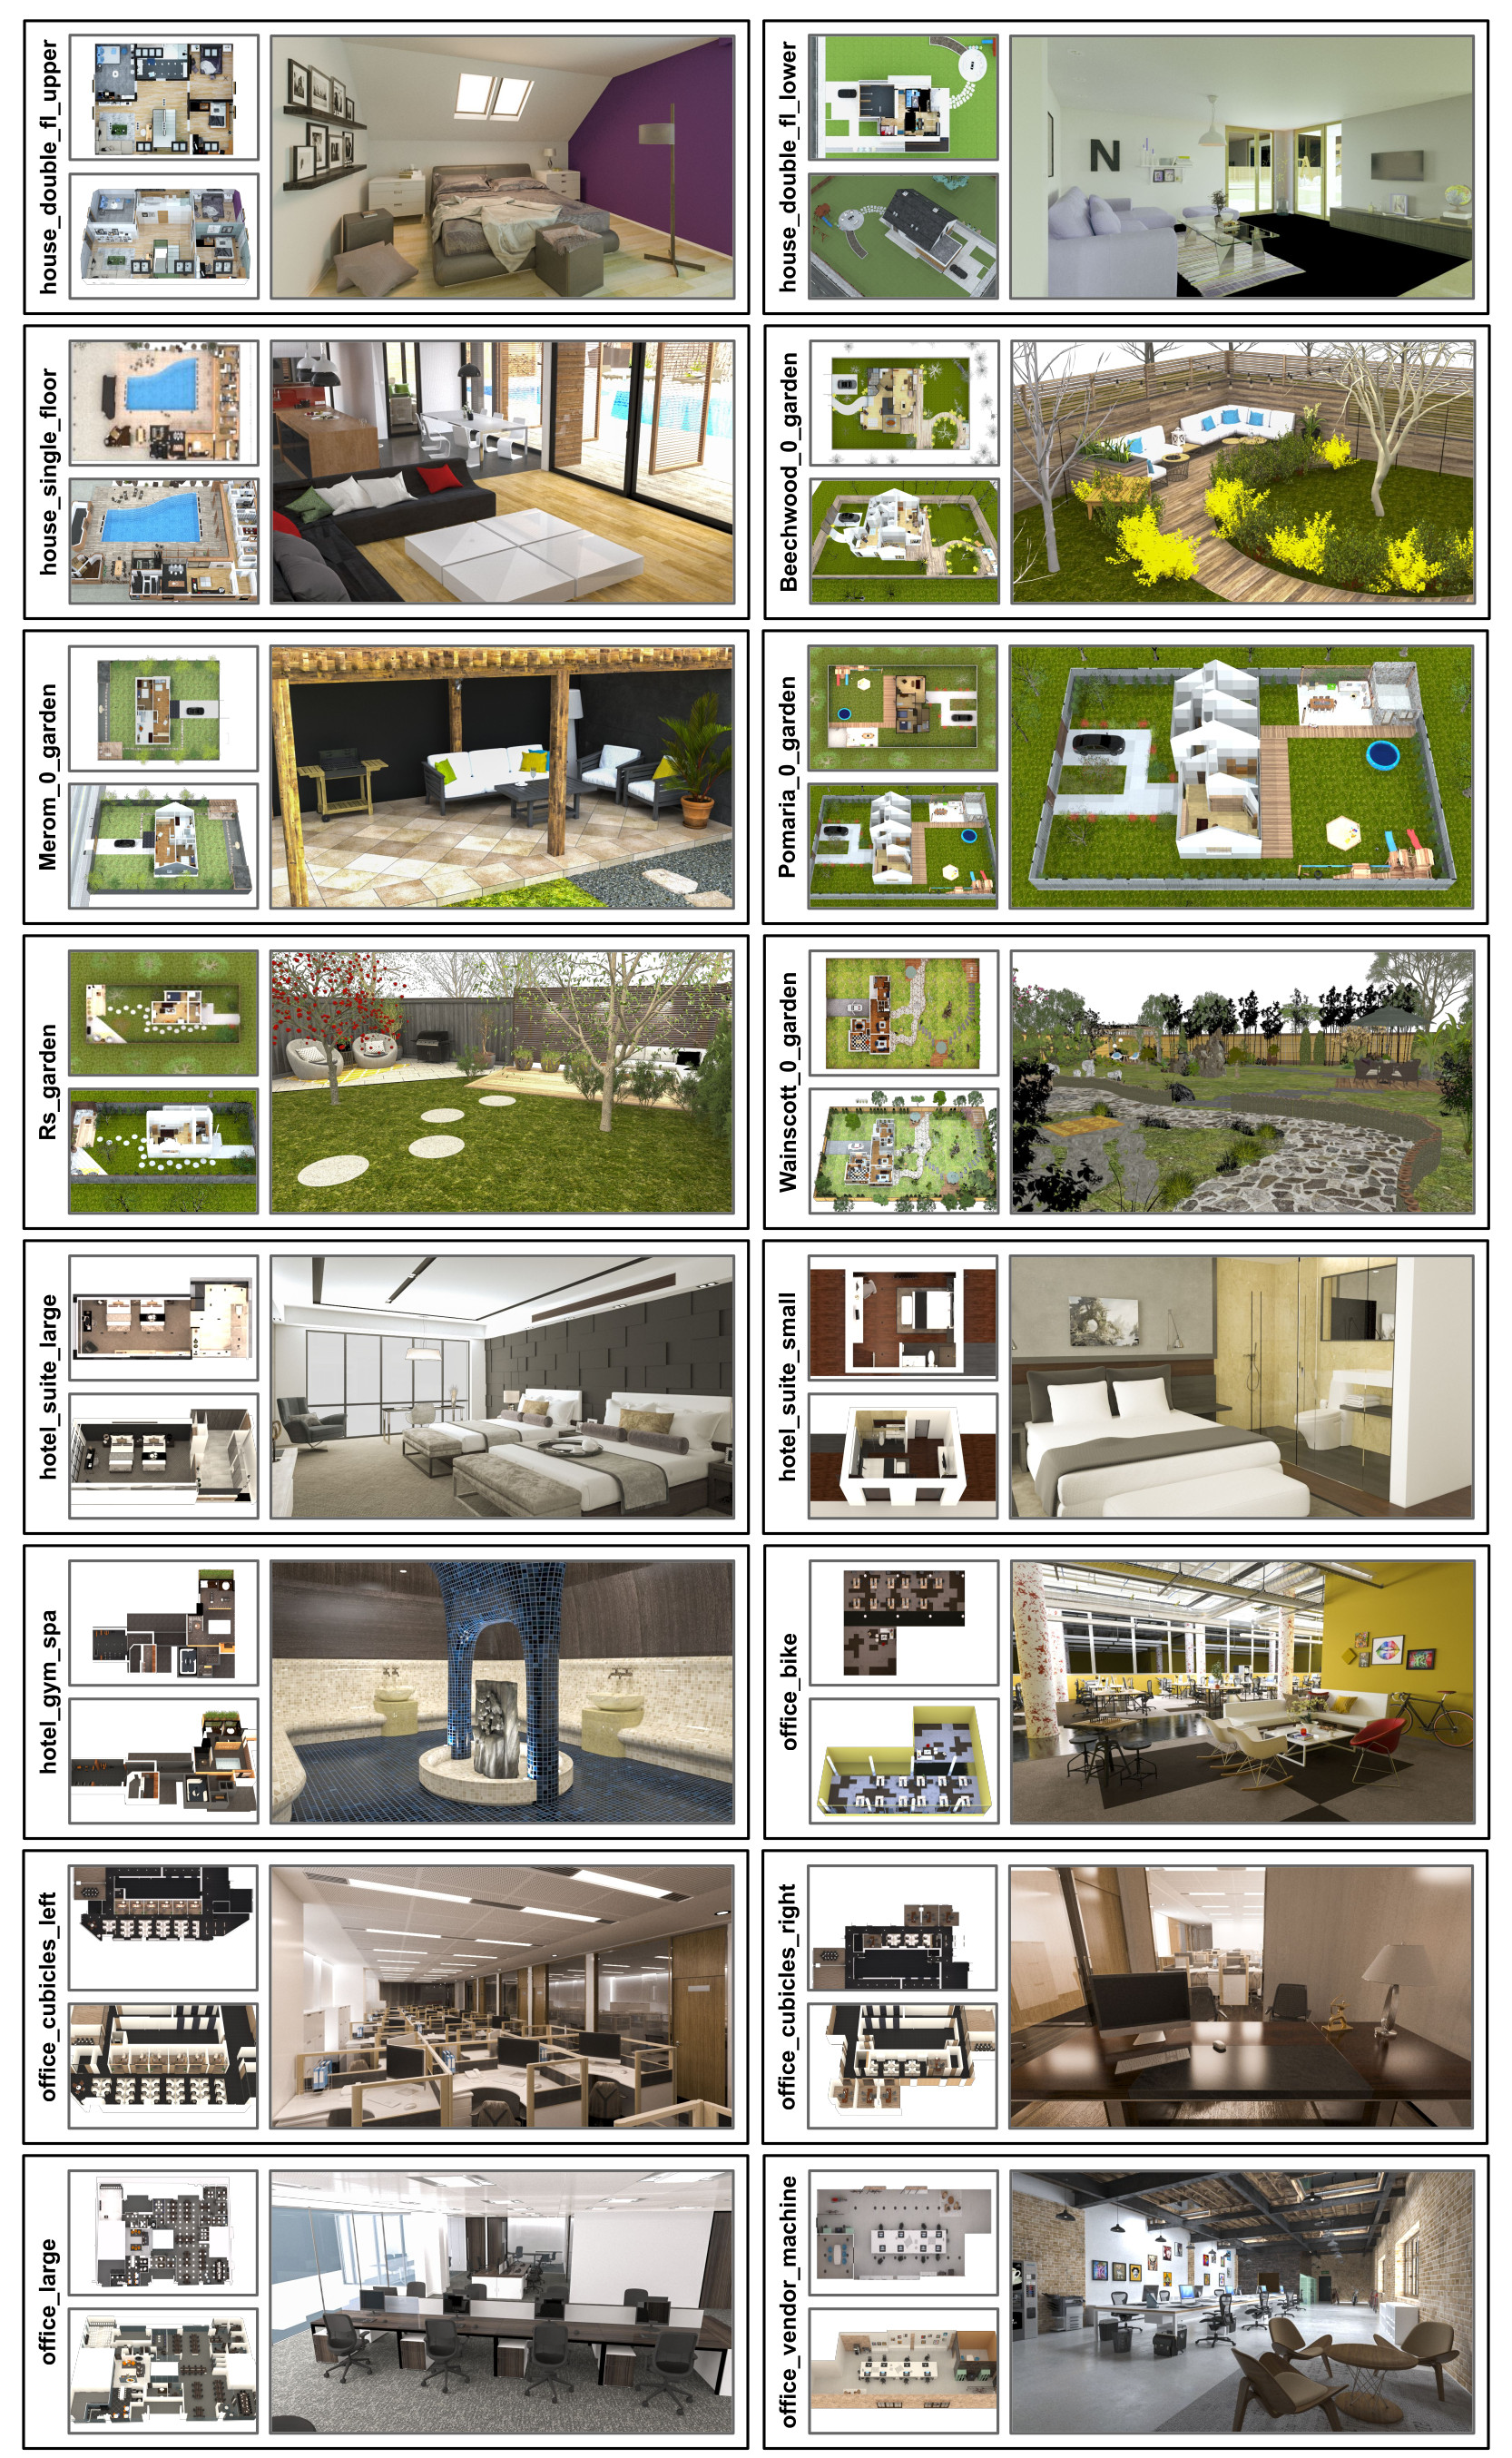
\includegraphics[width=\textwidth]{figures/models/scene_collage_p1.jpg}
    \caption{\revision{Part 1 of a scene collage showing views of all 50 scenes.}}
    %\label{fig:model_scene}
\end{figure}

\begin{figure}[th!]
    \centering
    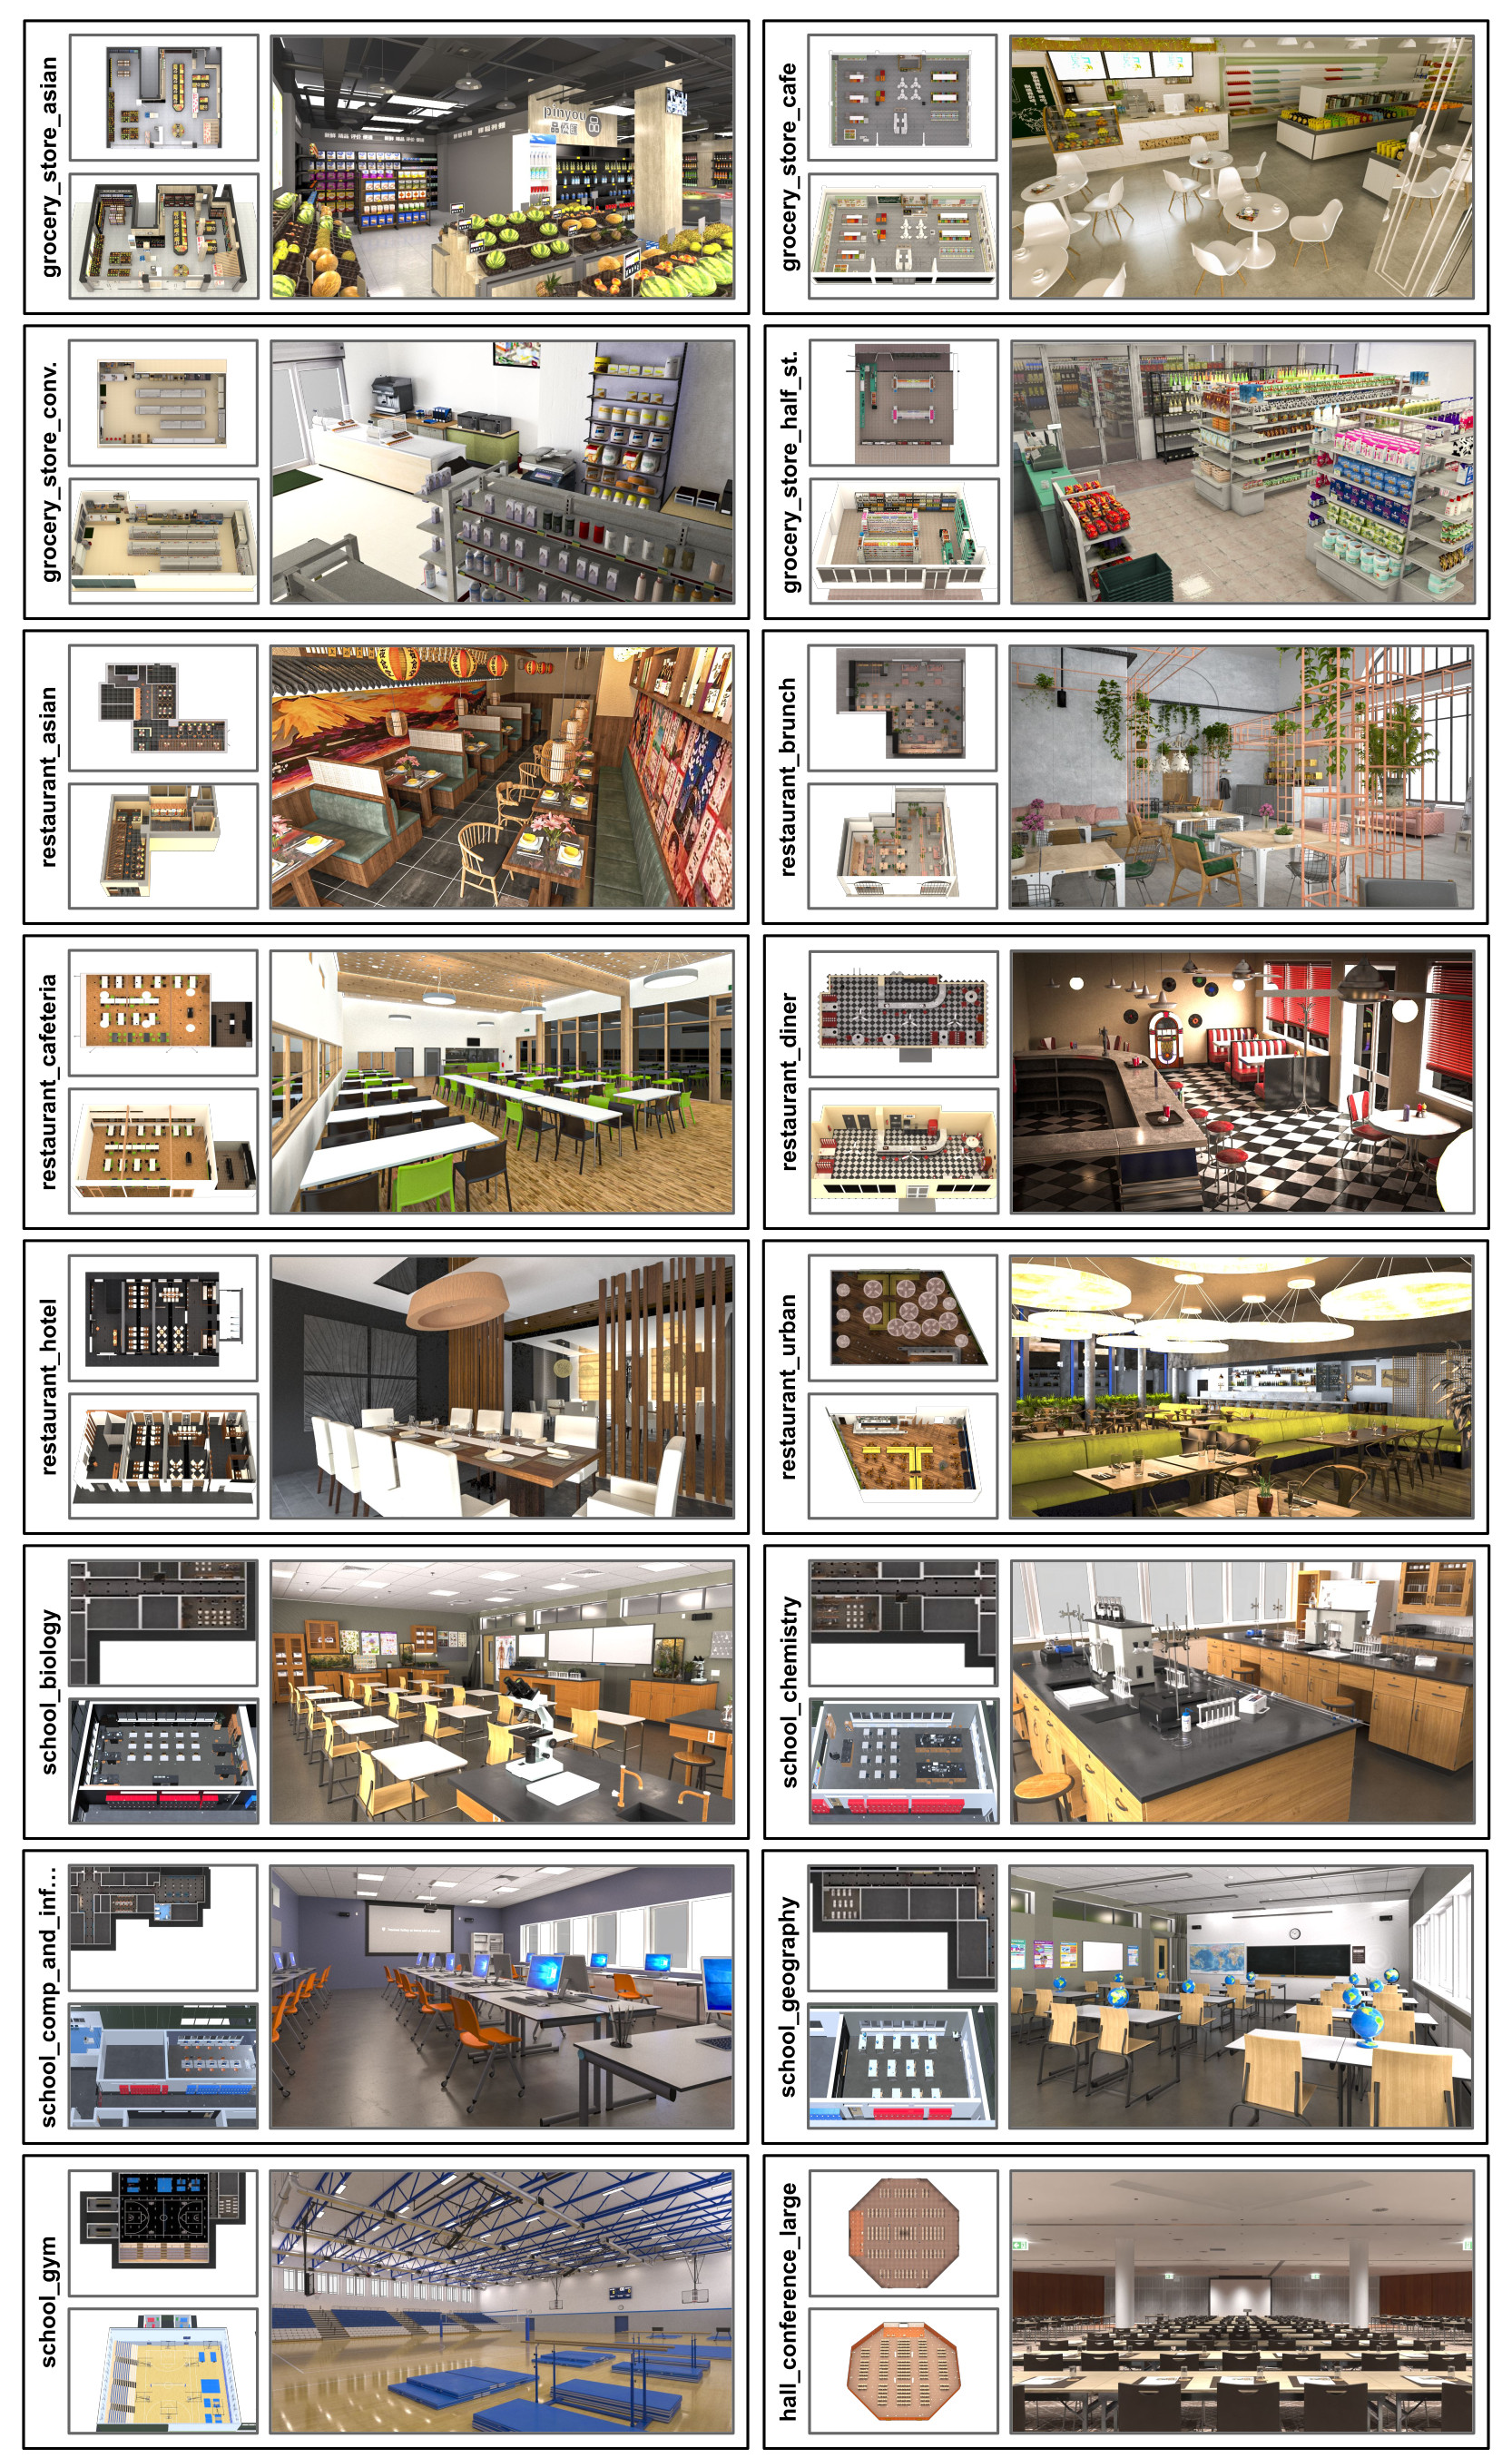
\includegraphics[width=\textwidth]{figures/models/scene_collage_p2.jpg}
    \caption{\revision{Part 2 of a scene collage showing views of all 50 scenes.}}
    %\label{fig:model_scene}
\end{figure}

\begin{figure}[th!]
    \centering
    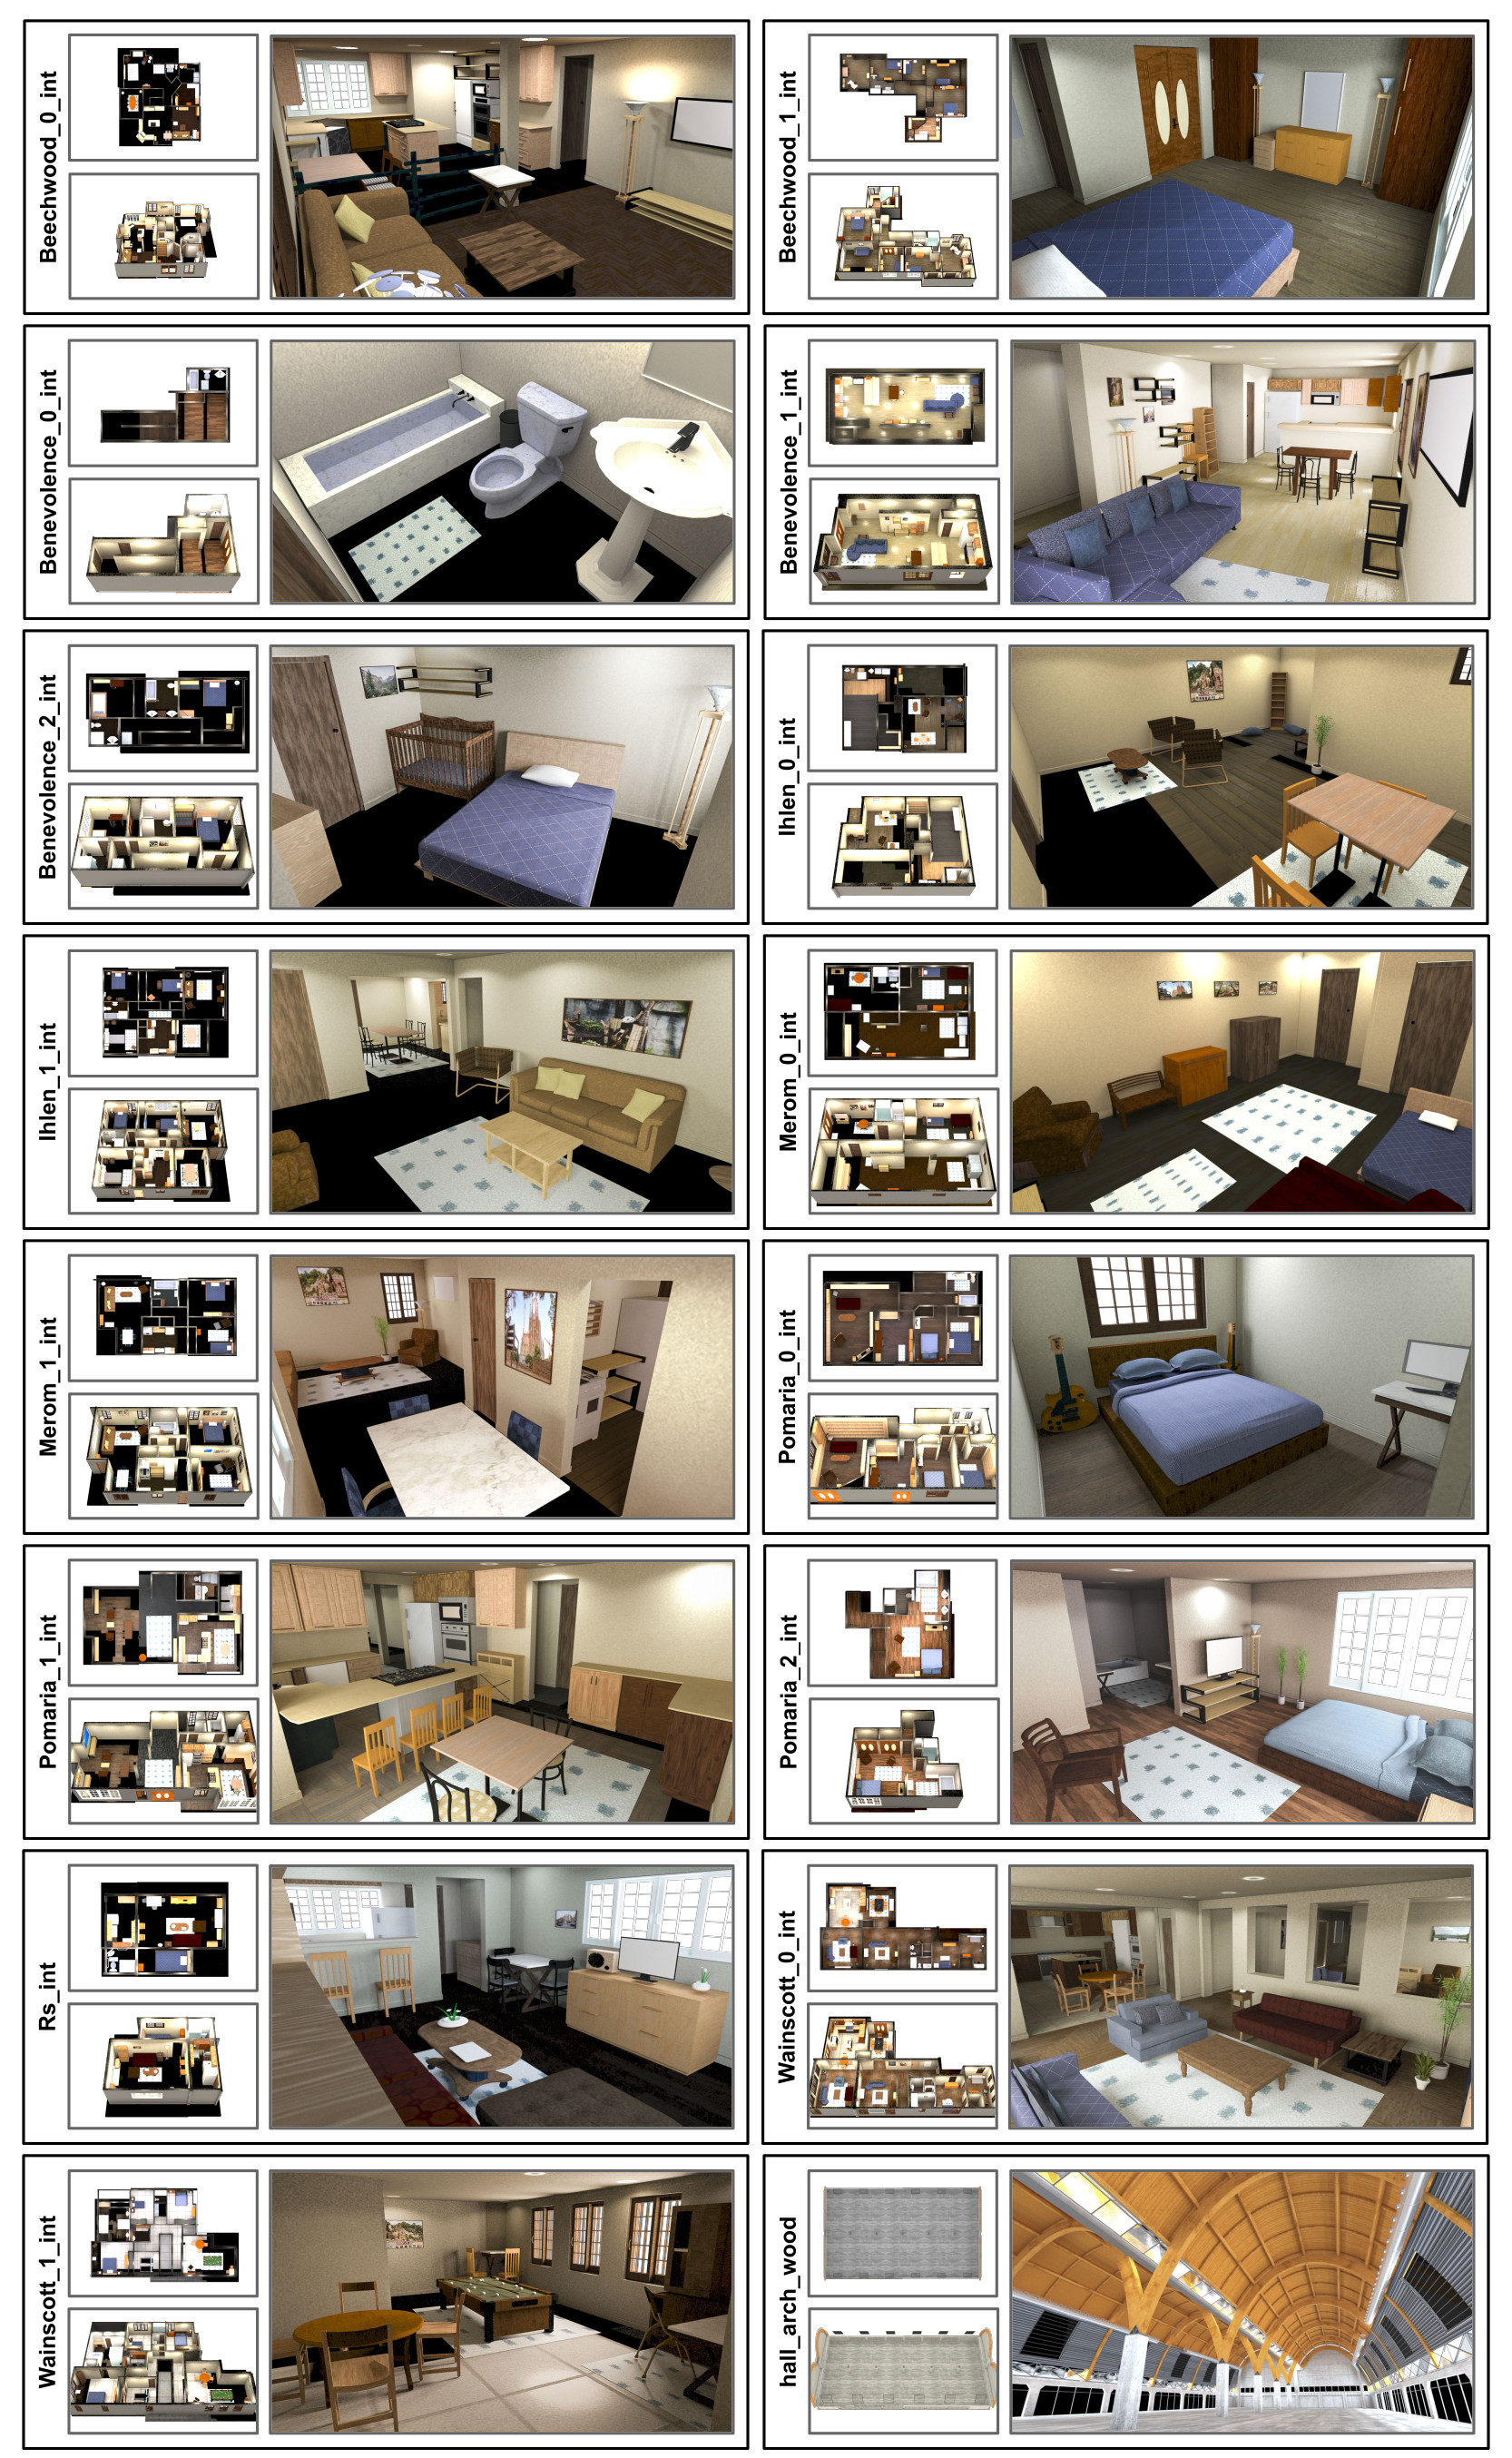
\includegraphics[width=\textwidth]{figures/models/scene_collage_p3.jpg}
    \caption{\revision{Part 3 of a scene collage showing views of all 50 scenes.}}
    %\label{fig:model_scene}
\end{figure}

\begin{figure}[th!]
    \centering
    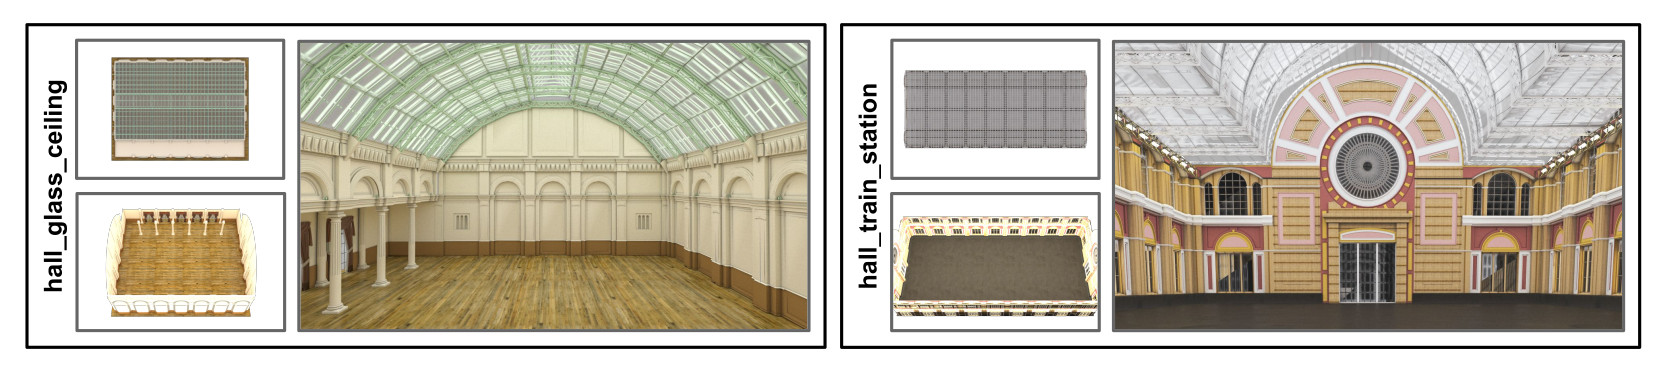
\includegraphics[width=\textwidth]{figures/models/scene_collage_p4.jpg}
    \caption{\revision{Part 4 of a scene collage showing views of all 50 scenes.}}
    %\label{fig:model_scene}
\end{figure}

\begin{figure}[th!]
 \centering
 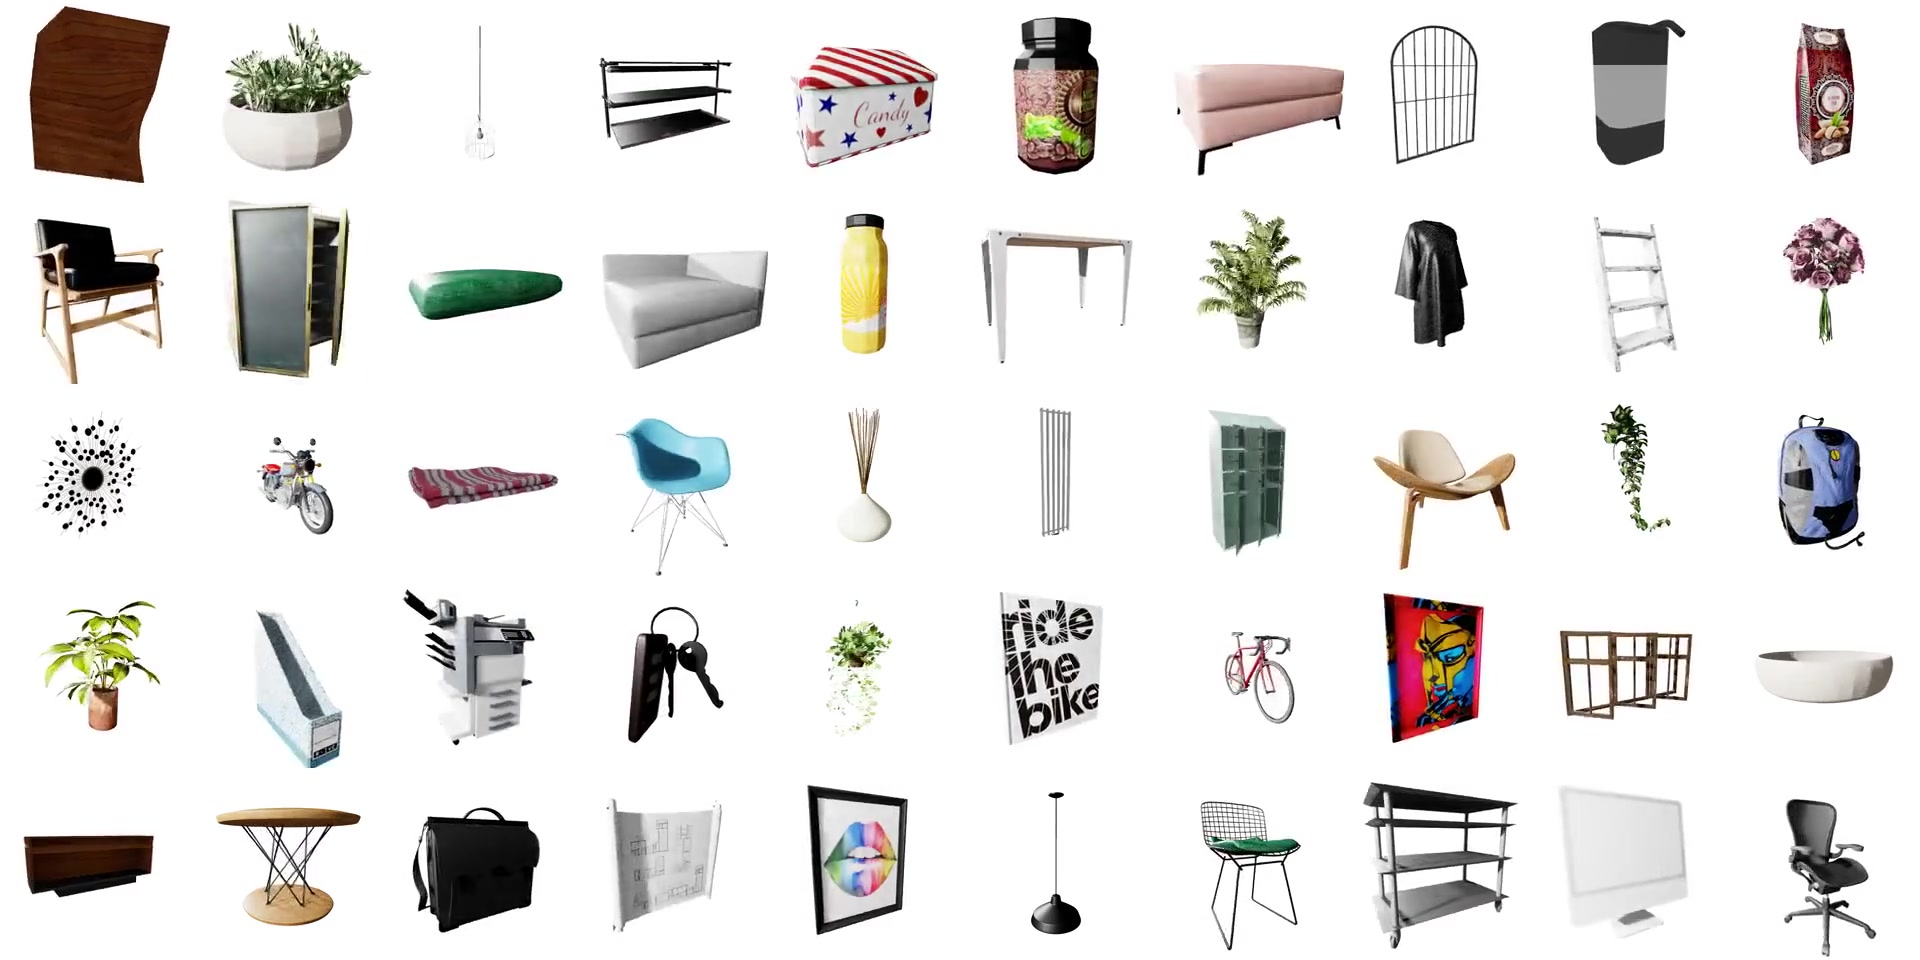
\includegraphics[width=0.9\textwidth]{figures/models/object_collage_3.jpg}
 \caption{\revision{A collage of objects included in the \dataset. These objects highlight key features of \simulator such as transparency, articulation, heat simulation, and lighting.}}
 \label{fig:model_object}
\end{figure}

\vspace{1.5cm}

{\scriptsize
\begin{longtable}{|m{.03\textwidth}|m{.16\textwidth}|m{.02\textwidth}|m{.02\textwidth}|m{.02\textwidth}|m{.27\textwidth}|m{.27\textwidth}|}
\hline
Scene Type
& Scene Name                            & Obj. Cnt.    & Syn. Cnt.    & Rm. Cnt.   & Room Types                                                                                                                                       & Example Activities                                                                                                                                                                                                                 \\ \hline
\multirow{15}{*}{\rotatebox[origin=c]{90}{\textbf{BEHAVIOR-100 Houses}}}
& Beechwood\_0\_int                     & 136          & 32           & 8          & \texttt{bathroom}, \texttt{corridor}, \texttt{dining\_room}, \texttt{entryway}, \texttt{kitchen}, \texttt{living\_room}, \texttt{private\_office}, \texttt{utility\_room}                                                & \texttt{clean a hot water dispenser}, \texttt{freeze lasagna}, \texttt{clean batting gloves}      \\ \cline{2-7} 
& Beechwood\_1\_int                     & 129          & 21           & 9          & \texttt{bathroom}, \texttt{bedroom}, \texttt{childs\_room}, \texttt{closet}, \texttt{corridor}, \texttt{playroom}, \texttt{television\_room }                                                                   & \texttt{clean your kitty litter box}, \texttt{store baby clothes}, \texttt{cleaning pet bed}      \\ \cline{2-7} 
& Benevolence\_0\_int                   & 21           & 10           & 4          & \texttt{bathroom}, \texttt{corridor}, \texttt{empty\_room}, \texttt{entryway}                                                                                                        & \texttt{laying clothes out}, \texttt{pack a pencil case}, \texttt{sweeping outside entrance}      \\ \cline{2-7} 
& Benevolence\_1\_int                   & 74           & 22           & 5          & \texttt{corridor}, \texttt{dining\_room}, \texttt{kitchen}, \texttt{living\_room}, \texttt{storage\_room}                                                                                     & \texttt{hanging blinds}, \texttt{sorting volunteer materials}, \texttt{wash baby bottles}      \\ \cline{2-7} 
& Benevolence\_2\_int                   & 63           & 23           & 5          & \texttt{bathroom}, \texttt{bedroom}, \texttt{corridor}                                                                                                                      & \texttt{clean walls}, \texttt{washing fabrics}, \texttt{folding clean laundry}      \\ \cline{2-7} 
& Ihlen\_0\_int                         & 68           & 21           & 7          & \texttt{bathroom}, \texttt{corridor}, \texttt{dining\_room}, \texttt{garage}, \texttt{living\_room}, \texttt{storage\_room}                                                                            & \texttt{de-clutter your garage}, \texttt{sorting household items}, \texttt{set up a home office in your garage}      \\ \cline{2-7} 
& Ihlen\_1\_int                         & 147          & 27           & 9          & \texttt{bathroom}, \texttt{bedroom}, \texttt{corridor}, \texttt{dining\_room}, \texttt{kitchen}, \texttt{living\_room}, \texttt{staircase}                                                                      & \texttt{clean jewels}, \texttt{clean green beans}, \texttt{hanging up curtains}      \\ \cline{2-7} 
& Merom\_0\_int                         & 82           & 27           & 6          & \texttt{bathroom}, \texttt{childs\_room}, \texttt{living\_room}, \texttt{playroom}, \texttt{storage\_room}, \texttt{utility\_room}                                                                     & \texttt{changing dog's water}, \texttt{wash a bra}, \texttt{wash a wool coat}      \\ \cline{2-7} 
& Merom\_1\_int                         & 123          & 28           & 8          & \texttt{bathroom}, \texttt{bedroom}, \texttt{childs\_room}, \texttt{corridor}, \texttt{dining\_room}, \texttt{kitchen}, \texttt{living\_room}, \texttt{staircase}                                                        & \texttt{store an uncooked turkey}, \texttt{drying table}, \texttt{clean flip flops}      \\ \cline{2-7} 
& Pomaria\_0\_int                       & 71           & 22           & 6          & \texttt{bathroom}, \texttt{bedroom}, \texttt{corridor}, \texttt{private\_office}, \texttt{television\_room }                                                                                  & \texttt{prepare sea salt soak}, \texttt{clean sheets}, \texttt{dispose of medication}      \\ \cline{2-7} 
& Pomaria\_1\_int                       & 89           & 24           & 6          & \texttt{bathroom}, \texttt{corridor}, \texttt{kitchen}, \texttt{living\_room}, \texttt{pantry\_room}, \texttt{utility\_room}                                                                           & \texttt{store brownies}, \texttt{clean a book}, \texttt{baking sugar cookies}      \\ \cline{2-7} 
& Pomaria\_2\_int                       & 42           & 18           & 3          & \texttt{bathroom}, \texttt{bedroom}, \texttt{corridor}                                                                                                                      & \texttt{replacing screens}, \texttt{clean baby toys}, \texttt{putting up posters}      \\ \cline{2-7} 
& Rs\_int                               & 72           & 32           & 5          & \texttt{bathroom}, \texttt{bedroom}, \texttt{entryway}, \texttt{kitchen}, \texttt{living\_room}                                                                                               & \texttt{dispose of a pizza box}, \texttt{putting food in fridge}, \texttt{putting out condiments}      \\ \cline{2-7} 
& Wainscott\_0\_int                     & 187          & 35           & 9          & \texttt{bathroom}, \texttt{bedroom}, \texttt{dining\_room}, \texttt{kitchen}, \texttt{living\_room}                                                                                           & \texttt{make microwave popcorn}, \texttt{make frozen lemonade}, \texttt{make cake mix}      \\ \cline{2-7} 
& Wainscott\_1\_int                     & 150          & 26           & 10         & \texttt{bathroom}, \texttt{bedroom}, \texttt{corridor}, exercise\_room, \texttt{playroom}, \texttt{private\_office}, \texttt{utility\_room}                                                            & \texttt{decorating for religious ceremony}, \texttt{stash snacks in your room}, \texttt{disinfect laundry}      \\ \hline
\multirow{5}{*}{\rotatebox[origin=c]{90}{{\textbf{BEHAVIOR-100 Houses+Garden}}}}
& Beechwood\_0\_garden                  & 335          & 45           & 9          & \texttt{bathroom}, \texttt{corridor}, \texttt{dining\_room}, \texttt{entryway}, \texttt{garden}, \texttt{kitchen}, \texttt{living\_room}, \texttt{private\_office}, \texttt{utility\_room}                                        & \texttt{tidy your garden}, \texttt{opening doors}, \texttt{wash goalkeeper gloves}      \\ \cline{2-7} 
& Merom\_0\_garden                      & 197          & 51           & 8          & \texttt{bathroom}, \texttt{childs\_room}, \texttt{garden}, \texttt{living\_room}, \texttt{playroom}, \texttt{sauna}, \texttt{storage\_room}, \texttt{utility\_room}                                                      & \texttt{clean your kitty litter box}, \texttt{clean a glass windshield}, \texttt{hang icicle lights}      \\ \cline{2-7} 
& Pomaria\_0\_garden                    & 260          & 49           & 7          & \texttt{bathroom}, \texttt{bedroom}, \texttt{corridor}, \texttt{garden}, \texttt{private\_office}, \texttt{television\_room }                                                                          & \texttt{putting up Christmas lights outside}, \texttt{prepare a hanging basket}, \texttt{clean a patio}      \\ \cline{2-7} 
& Rs\_garden                            & 185          & 47           & 6          & \texttt{bathroom}, \texttt{bedroom}, \texttt{entryway}, \texttt{garden}, \texttt{kitchen}, \texttt{living\_room}                                                                                       & \texttt{cleaning driveway}, \texttt{clean a longboard}, \texttt{roast nuts}      \\ \cline{2-7} 
& Wainscott\_0\_garden                  & 712          & 61           & 10         & \texttt{bathroom}, \texttt{bedroom}, \texttt{dining\_room}, \texttt{garden}, \texttt{kitchen}, \texttt{living\_room}                                                                                   & \texttt{clean an espresso machine}, \texttt{clearing food from table into fridge}, \texttt{painting porch}      \\ \hline
\multirow{3}{*}{\rotatebox[origin=c]{90}{\textbf{New Houses}}}
& house\_single\_floor                  & 1375         & 137          & 23         & \texttt{bathroom}, \texttt{bedroom}, \texttt{childs\_room}, \texttt{closet}, \texttt{corridor}, \texttt{dining\_room}, \texttt{empty\_room}, \texttt{entryway}, \texttt{garden}, \texttt{kitchen}, \texttt{living\_room}, \texttt{sauna}, \texttt{utility\_room}      & \texttt{turning out all lights before sleep}, \texttt{iron curtains}, \texttt{packing hobby equipment}      \\ \cline{2-7} 
& {\tiny house\_double\_floor\_lower}   & 304          & 79           & 6          & \texttt{bathroom}, \texttt{corridor}, \texttt{garage}, \texttt{garden}, \texttt{kitchen}, \texttt{living\_room}                                                                                        & \texttt{wash towels}, \texttt{clean a fish}, \texttt{clean brass}      \\ \cline{2-7} 
& {\tiny house\_double\_floor\_upper}   & 325          & 78           & 5          & \texttt{bathroom}, \texttt{bedroom}, \texttt{television\_room }                                                                                                             & \texttt{clean a saxophone}, \texttt{taking down curtains}, \texttt{clean walls}      \\ \hline
\multirow{4}{*}{\rotatebox[origin=c]{90}{\textbf{Grocery Stores}}}
& grocery\_store\_asian                 & 3402         & 79           & 2          & \texttt{bathroom}, \texttt{grocery\_store}                                                                                                                         & \texttt{buy alcohol}, \texttt{buy boxes for packing}, \texttt{buy a microwave oven}      \\ \cline{2-7} 
& grocery\_store\_cafe                  & 6994         & 71           & 4          & \texttt{bar} , \texttt{bathroom}, \texttt{dining\_room}, \texttt{grocery\_store}                                                                                                      & \texttt{defrost meat}, \texttt{clean reusable shopping bags}, \texttt{buy a good avocado}      \\ \cline{2-7} 
& {\tiny grocery\_store\_convenience}   & 1889         & 82           & 2          & \texttt{bathroom}, \texttt{grocery\_store}                                                                                                                         & \texttt{washing windows}, \texttt{picking up prescriptions}, \texttt{buy food for vegetarians}      \\ \cline{2-7} 
& {\tiny grocery\_store\_half\_stocked} & 3804         & 51           & 2          & \texttt{bathroom}, \texttt{grocery\_store}                                                                                                                         & \texttt{buying gardening supplies}, \texttt{buy basic garden tools}, \texttt{buy boxes for packing}      \\ \hline
\multirow{4}{*}{\rotatebox[origin=c]{90}{\textbf{Halls}}}
& hall\_arch\_wood                      & 78           & 11           & 2          & \texttt{bathroom}, \texttt{empty\_room}                                                                                                                         &    \texttt{clean walls}  \\ \cline{2-7} 
& hall\_train\_station                  & 141          & 15           & 2          & \texttt{bathroom}, \texttt{empty\_room}                                                                                                                            &  \texttt{clean cement}    \\ \cline{2-7} 
& hall\_glass\_ceiling                  & 116          & 20           & 2          & \texttt{bathroom}, \texttt{empty\_room}                                                                                                                            &  \texttt{preparing food for a fundraiser}   \\ \cline{2-7} 
& hall\_conference\_large               & 3372         & 26           & 2          & \texttt{bathroom}, \texttt{conference\_hall}                                                                                                                       &  \texttt{distributing event T-shirts}    \\ \hline
\multirow{3}{*}{\rotatebox[origin=c]{90}{\textbf{Hotels}}}
& hotel\_gym\_spa                       & 322          & 43           & 9          & \texttt{bathroom}, \texttt{corridor}, \texttt{gym} , \texttt{hammam} , \texttt{locker\_room} , \texttt{sauna}, \texttt{spa}                                                                                         & \texttt{turning on the hot tub}, \texttt{adding chemicals to hot tub}, \texttt{clean a sauna}      \\ \cline{2-7}
& hotel\_suite\_large                   & 218          & 51           & 2          & \texttt{bathroom}, \texttt{bedroom}                                                                                                                                & \texttt{clean vinyl shutters}, \texttt{cleaning computer}, \texttt{clean white marble}      \\ \cline{2-7} 
& hotel\_suite\_small                   & 48           & 28           & 2          & \texttt{bathroom}, \texttt{bedroom}                                                                                                                                & \texttt{clean cork mats}, \texttt{putting out clean towels}, \texttt{clean a shower}      \\ \hline
\multirow{5}{*}{\rotatebox[origin=c]{90}{\textbf{Offices}}}
& office\_bike                          & 479          & 49           & 3          & \texttt{bathroom}, \texttt{break\_room}, \texttt{shared\_office}                                                                                                            & \texttt{set up a webcam}, \texttt{set up two computer monitors}, \texttt{clean an office chair}      \\ \cline{2-7} 
& office\_cubicles\_left                & 787          & 44           & 12         & \texttt{bathroom}, \texttt{conference\_hall}, \texttt{copy\_room}, \texttt{corridor}, \texttt{lobby}, \texttt{meeting\_room}, \texttt{private\_office}, \texttt{shared\_office}                                          & \texttt{clean up your desk}, \texttt{clean a LED screen}, \texttt{laying out snacks at work}      \\ \cline{2-7} 
& office\_cubicles\_right               & 406          & 37           & 11         & \texttt{bathroom}, \texttt{conference\_hall}, \texttt{copy\_room}, \texttt{corridor}, \texttt{lobby}, \texttt{meeting\_room}, \texttt{private\_office}, \texttt{shared\_office}                                          & \texttt{making photocopies}, \texttt{clean a LED screen}, \texttt{clean a keyboard}      \\ \cline{2-7} 
& office\_large                         & 1151         & 46           & 24         & \texttt{bathroom}, \texttt{break\_room}, \texttt{conference\_hall}, \texttt{copy\_room}, \texttt{corridor}, \texttt{lobby}, \texttt{meeting\_room}, \texttt{phone\_room}, \texttt{private\_office}, \texttt{shared\_office}                & \texttt{emptying trash cans}, \texttt{putting meal in fridge at work}, \texttt{brewing coffee}      \\ \cline{2-7} 
& office\_vendor\_machine               & 225          & 45           & 4          & \texttt{bathroom}, \texttt{break\_room}, \texttt{meeting\_room}, \texttt{shared\_office}                                                                                             & \texttt{clean a computer monitor}, \texttt{make the workplace exciting}, \texttt{dispose of glass}      \\ \hline
\multirow{6}{*}{\rotatebox[origin=c]{90}{\textbf{Restaurants}}}
& restaurant\_asian                     & 1221         & 56           & 3          & \texttt{bathroom}, \texttt{dining\_room}, \texttt{kitchen}                                                                                                                  & \texttt{grill vegetables}, \texttt{cook tofu}, \texttt{clean clams}      \\ \cline{2-7} 
& restaurant\_brunch                    & 1096         & 70           & 4          & \texttt{bar} , \texttt{bathroom}, \texttt{dining\_room}, \texttt{kitchen}                                                                                                             & \texttt{stock a bar}, \texttt{cook squid}, \texttt{washing vegetables}      \\ \cline{2-7} 
& restaurant\_cafeteria                 & 292          & 45           & 3          & \texttt{bathroom}, \texttt{dining\_room}, \texttt{kitchen}                                                                                                                  & \texttt{clean a popcorn machine}, \texttt{store coffee beans or ground coffee}, \texttt{roast meat}      \\ \cline{2-7} 
& restaurant\_diner                     & 174          & 39           & 3          & \texttt{bar} , \texttt{bathroom}, \texttt{dining\_room}                                                                                                                      & \texttt{sweeping floors}, \texttt{installing smoke detectors}, \texttt{clean a lobster}      \\ \cline{2-7} 
& restaurant\_hotel                     & 1080         & 81           & 4          & \texttt{bathroom}, \texttt{dining\_room}, \texttt{kitchen}, \texttt{lobby}                                                                                                           & \texttt{clean eggs}, \texttt{setting table for coffee}, \texttt{clean a pizza stone}      \\ \cline{2-7}
& restaurant\_urban                     & 1368         & 90           & 4          & \texttt{bar} , \texttt{bathroom}, \texttt{dining\_room}, \texttt{kitchen}                                                                                                             & \texttt{cook pumpkin seeds}, \texttt{putting roast in oven}, \texttt{thaw frozen fish}      \\ \hline
\multirow{5}{*}{\rotatebox[origin=c]{90}{\textbf{Schools}}}
& school\_biology                       & 717          & 53           & 4          & \texttt{bathroom}, \texttt{biology\_lab} , \texttt{corridor}                                                                                                                 & \texttt{clean an eraser}, \texttt{turning sprinkler off}, \texttt{clean a glass pipe}      \\ \cline{2-7} 
& school\_chemistry                     & 890          & 69           & 4          & \texttt{bathroom}, \texttt{chemistry\_lab} , \texttt{corridor}                                                                                                               & \texttt{clean clear plastic}, \texttt{clean an eraser}, \texttt{clean a whiteboard}      \\ \cline{2-7} 
& {\tiny school\_comp\_lab\_infirmary}  & 828          & 61           & 6          & \texttt{bathroom}, \texttt{computer\_lab}, \texttt{corridor}, \texttt{infirmary}                                                                                                     & \texttt{clean a computer monitor}, \texttt{prepare an emergency school kit}, \texttt{clean a keyboard}      \\ \cline{2-7} 
& school\_geography                     & 556          & 42           & 5          & \texttt{bathroom}, \texttt{classroom}, \texttt{corridor}                                                                                                                    & \texttt{clean gold}, \texttt{clean a glass pipe}, \texttt{clean an eraser}      \\ \cline{2-7} 
& school\_gym                           & 853          & 36           & 7          & \texttt{bathroom}, \texttt{corridor}, \texttt{gym} , \texttt{locker\_room}                                                                                                             & \texttt{clean a dirty baseball}, \texttt{dispose of glass}, \texttt{wash towels}      \\ \hline

\caption{Statistics and information for each of 50 scenes in B1K: scene type, name, number of objects, unique synsets and rooms, room types, and example activities }
\label{tab:model_scene}
\end{longtable}
}




% Furthermore, the diversity of the activities in our new environments (such as cleaning in offices, or cooking in restaurants) requires certain types of rooms (e.g. public restrooms and commercial kitchens) to be present in the scenes, which is not typically the case for available models. To support these use cases, 5 public restroom models and 2 commercial kitchen models were separately acquired from Turbosquid, and attached to non-house scenes as necessary, with pairings being made based on visual compatibility. The seamless integration of these partial scenes into the larger scenes also allows the reuse of objects across the scenes while still representing the diversity of such environments. Another important requirement that arose from the survey results was that the participants consistently want robots to help with outdoor activities (e.g. gardening, shoveling snow, etc.), which cannot be simulated in the indoor-only \oldbenchmark scenes. To resolve this, the \dataset contains both entirely new houses that have gardens, as well as augmented versions of \oldbenchmark houses that have gardens attached. These gardens, diverse in terms of both size and features, were also separately acquired from TurboSquid, and were attached to the house scenes by professional architects that were contracted on Upwork. Exterior walls were also added to the previously indoor-only houses, representing a variety of architectural styles that are prevalent globally.


% To be imported into \simulator, scene and object models that were acquired from online marketplaces were processed by members of our team through a purpose-built annotation process in Autodesk 3ds Max, designed to correctly label each object's articulations, lights, and other features such as heating and toggling, as well as scene features such as room boundaries. Accurate labeling of canonical orientations and equally-granular categories (as well as whether certain objects should not be randomized) for each object, a critical requirement of the Object Randomization feature supported in \simulator, was also undertaken at this stage. The processed scene files were then run through our automated 3ds Max-to-\simulator pipeline, which exports the objects, their materials (including compatible features such as transparency and self-illumination), their joint configurations, and additional features as well as generating additional metadata (e.g. minimum-value bounding boxes) and checking for physics stability.
\section{Simulation}

\subsection{Extended Object States and Logical Predicates in \simulator}
\label{as:object_states}
\simulator extends the infrastructure of extended object states and logical predicates from iGibson 2.0~\cite{li2021ig2} to accommodate the diversity and realism of \benchmark.

\subsubsection{Extended object states associated with object category properties}
For computational efficiency purposes, not all extended object states need to be maintained and updated for every object. For example, \texttt{cookable} objects like apples need to keep track of their \texttt{Temperature}, but probably tables don't need to, at least for the purpose of simulating \benchmark activities. Hence, given the object category property annotation from \dataset (see Table~\ref{tab:supp_props}), \simulator selectively keeps track of a subset of the extended states for objects of each category. The mapping from the object category property to the required object states can be found in Table~\ref{table:obj_cat_prop}.
\begin{table}[!htbp]
\begin{center}
{%
\scriptsize
\renewcommand{\arraystretch}{1.2}
\begin{tabular}{ | m{3.5cm} | m{3.7cm} | } 
\hline
\textbf{Object category property} & \textbf{Required extended object states}\\ 
\hline
\texttt{cookable} & \texttt{MaxTemperature}, \texttt{Temperature}\\ 
\hline
\texttt{overcookable} & \texttt{MaxTemperature}, \texttt{Temperature}\\ 
\hline
\texttt{freezable} & \texttt{Temperature}\\ 
\hline
\texttt{flammable} & \texttt{Temperature}\\ 
\hline
\texttt{heatable} & \texttt{Temperature}\\ 
\hline
\texttt{metable} & \texttt{Temperature}\\ 
\hline
\texttt{soakable} & \texttt{SoakedLevel}\\ 
\hline
\texttt{toggleable} & \texttt{ToggledState}\\ 
\hline
\texttt{sliceable} & \texttt{SlicedState}\\ 
\hline
\texttt{breakable} & \texttt{BrokenState}\\ 
\hline
\texttt{heatSource} & \texttt{ToggledState}\\ 
\hline
\texttt{fireSource} & \texttt{ToggledState}\\ 
\hline
\texttt{coldSource} & \texttt{ToggledState}\\ 
\hline
\texttt{waterSource} & \texttt{ToggledState}\\ 
\hline
\end{tabular}
}
\vspace{3pt}
\caption{Extended object states associated with object category properties. Adapted from~\cite{li2021ig2}.}
\label{table:obj_cat_prop}
\end{center}
\end{table}

\subsubsection{Object model properties}
We also need to perform physical and semantic annotation for each object model so that they can be realistically simulated and support the evolution of extended object states. Some of the physical properties can be programmatically generated from the 3D assets, such as \texttt{Shape}, \texttt{KinematicStructure} and  \texttt{StableOrientations}, while others need to be annotated (included in \dataset), such as \texttt{Weight}. \texttt{Type} of an object model, which is also derived from the object category property annotation from \dataset (see Table~\ref{tab:supp_props}), determines how the object will be simulated in \simulator. For example, cloths and fluids will be simulated using underlying particle systems. Also, some of the object category property requires additional semantic annotation for each model of that category, e.g. for \texttt{waterSource} objects, \texttt{WaterSourceLink} is required to indicate the exact location to generate water. An exhaustive list of all the object model properties can be found in Table~\ref{table:obj_model_prob}.
\begin{table}[!htbp]
\begin{center}
%\resizebox{\textwidth}{!}
{%
\scriptsize
\renewcommand{\arraystretch}{1.2}
\begin{tabular}{ | m{2.5cm} | m{2.7cm} | m{7.5cm} | } 
\hline
\textbf{Object model property} & \textbf{Relevant object category property} & \textbf{Description} \\ 
\hline
\texttt{Shape} &  & Model of the 3D shape of each link of the object\\ 
\hline
\texttt{Weight} &  & Weight of the object \\ 
\hline
\texttt{CenterOfMass} &  & Mean position of the matter in the object\\ 
\hline
\texttt{MomentOfInertia} &  & Resistance of the object to change its angular velocity\\ 
\hline
\texttt{KinematicStructure} &  & Structure of links and joints connecting them in the form of URDF (non-articulated objects are composed of one link)\\ 
\hline
\texttt{StableOrientations} &  & A list of stable orientations assuming the object is placed on a flat surface, computed using a 3D geometry library\\ 
\hline
\texttt{HeatSourceLink} & \texttt{heatSource} & Virtual (non-colliding) fixed link that generates heat\\
\hline
\texttt{FireSourceLink} & \texttt{fireSource} & Virtual (non-colliding) fixed link that generates fire\\
\hline
\texttt{CleaningToolLink} & \texttt{cleaningTool} & Fixed link that needs to contact dirt particles for the tool to clean them\\ 
\hline
\texttt{WaterSourceLink} &  \texttt{waterSource} & Virtual (non-colliding) fixed link that generates water\\
\hline
\texttt{WaterSinkLink} &  \texttt{waterSource} & Virtual (non-colliding) fixed link that absorbs water\\ 
\hline
\texttt{TogglingLink} &  \texttt{toggleable} & Virtual (non-colliding) fixed link that changes the toggled state of the object when contacted\\ 
\hline
\texttt{SlicingLink} & \texttt{slicingTool} & Fixed link that changes the sliced state of another object if it contacts it with enough force\\ 
\hline
\texttt{RelevantJoints} & \texttt{openable} & List of joints that are relevant to indicate whether an object is open\\ 
\hline
\texttt{AttachmentKeypoints} & \texttt{assembleable} & List of keypoint locations that will be connected with those of other objects when they are close enough\\ 
\hline
\texttt{ClothKeypoints} & \texttt{foldable}, \texttt{unfoldable} & List of keypoint locations are used to determine if the object is folded (if they are close enough) or unfolded (if they are far enough)\\ 
\hline
\texttt{ContainerVolume} & \texttt{fillable} & Virtual (non-colliding) fixed link that represents the inner volume of a fillable container.\\ 
\hline
\texttt{Type} & \texttt{cloth}, \texttt{deformable}, \texttt{liquid}, \texttt{rope}, \texttt{physicalSubstance}, \texttt{visualSubstance}  & Type of the object, e.g. rigid body, fluid, physical/visual substance, cloth, deformable, which determines how it will be simulated in \simulator \\ 
\hline
\end{tabular}
}
\vspace{3pt}
\caption{Permanent object model properties. Adapted from~\cite{li2021ig2}.}
\label{table:obj_model_prob}
\end{center}
\end{table}

\subsubsection{Object states}
While the object properties mentioned above stay the same during simulation (i.e. an apple is always \texttt{cookable} and a sink always have the same \texttt{WaterSourceLink} defined in its local frame), the object states could change. The underlying physics engine handles the kinematic state changes, such as \texttt{Pose}, \texttt{AABB}, \texttt{JointStates}, \texttt{ParticlePositions} for fluids and cloths, etc. On top of these, \simulator handles the non-kinematic state changes that are essential for logical predicates (described in the next subsection). For example, \simulator update the \texttt{Temperature} of objects at every simulation step by checking if they are near/inside any \texttt{heatSource} or \texttt{coldSource}. An exhaustive list of all the object states can be found in Table~\ref{table:obj_states}.
\begin{table}[!htbp]
\begin{center}
%\resizebox{\textwidth}{!}
{\scriptsize%
\renewcommand{\arraystretch}{1.2}
\begin{tabular}{ | m{4cm} | m{9cm} | } 
\hline
\textbf{Object State} & \textbf{Description and Update Rules} \\ 
\hline
\texttt{Pose} & 6 DoF pose (position and orientation) of the object in world reference frame, updated by the underlying physics engine.\\ 
\hline
\texttt{AABB} & Axis-aligned bounding box (coordinates of two opposite corners) of the object in the world reference frame, updated by the underlying physics engine.\\ 
\hline
\texttt{JointStates} & State of all internal DoFs of the (articulated) object for the structure defined by \texttt{KinematicStructure}, updated by the underlying physics engine.\\ 
\hline
\texttt{ParticlePositions} & Positions of all the underlying particles for cloth and fluid, updated by the underlying physics engine.\\ 
\hline
\texttt{InContactObjs} & List of all objects in physical contact with the object, updated by the underlying physics engine.\\ 
\hline
\texttt{ConnectedObjs} & List of all objects that are connected to the object, either via a fixed joint for rigid bodies or via an attachment for cloth and deformables.\\ 
\hline
\texttt{InSamePositiveVerticalAxisObjs} & List of all objects in the positive vertical axis drawn from the object's center of mass, updated by shooting a ray upwards in the positive z-axis and gather the objects hit by the ray.\\ 
\hline
\texttt{InSameNegativeVerticalAxisObjs} & List of all objects in the negative vertical axis drawn from the object's center of mass, updated by shooting a ray downwards in the negative z-axis and gather the objects hit by the ray.\\ 
\hline
\texttt{InSameHorizontalPlaneObjs} & List of all objects in the horizontal plane drawn from the object's center of mass, updated by shooting a number of ray in the x-y plane and gather the objects hit by the rays.\\ 
\hline
\texttt{Temperature}, $T$ & Object's current temperature in $^\circ$C, updated by detecting if the object is affected by any heat source or heat sink.\\ 
\hline
\texttt{MaxTemperature}, $T_\textit{max}$ & Maximum temperature of the object reached historically during this simulation run, updated by keeping track of all the \texttt{Temperature} in the history.\\ 
\hline
\texttt{SoakedLevel}, $w$ & Amount of liquid absorbed by the object corresponding to the number of liquid particles contacted, updated by detecting if the object is in contact with any liquid particle. This is maintained for every type of \texttt{liquid} separately. \\ 
\hline
\texttt{CoveredLevel}, $c$ & Amount of \texttt{visualSubstance} that covers the object, updated by detecting if the particles of the \texttt{visualSubstance} are in contact with anything that can potentially remove them from the object, e.g. \texttt{cleaningTool}. This is maintained for every type of \texttt{visualSubstance} separately. \\ 
\hline
% \texttt{DustinessLevel}, $d$ & Fraction of the initial amount of dust particles that remain on the object's surface, updated by detecting if the particles are in contact with any \texttt{CleaningTool}.\\ 
% \hline
% \texttt{StainLevel}, $s$ & Fraction of the initial amount of stain particles that remain on the object's surface, updated by detecting if the particles are in contact with any \texttt{Soaked} \texttt{CleaningTool}.\\ 
% \hline
\texttt{ToggledState}, $\textit{TS}$ & Binary state indicating if the object is currently on or off, updated by detecting if the agent is in contact with the \texttt{TogglingLink}.\\ 
\hline
\texttt{SlicedState}, $\textit{SS}$ & Binary state indicating whether the object has been sliced (irreversible), updated by detecting if the object is in contact with any \texttt{SlicingTool} that exerts a force above a certain threshold $F_\mathit{sliced}$. We assume as default force threshold of $F_\mathit{sliced} = \SI{10}{\newton}$, a value that can be configured per object category and model.\\ 
\hline
\texttt{BrokenState}, $\textit{BS}$ & Binary state indicating if the object is broken, updated by detecting if the object has a contact force with any other object above a certain threshold $F_\mathit{broken}$, a value that can be configured per object category and model.\\ 
\hline
\end{tabular}
}
\vspace{3pt}
\caption{Object states maintained by \simulator. Adapted from~\cite{li2021ig2}.}
\label{table:obj_states}
\end{center}
\end{table}

\subsubsection{Logical predicates as checking functions}
For each logical predicate that is relevant for \benchmark activities, we define a checking function that maps a given physical state (kinematic and non-kinematic) into a binary logical state that \bddl operates on. For example, \texttt{OnTopOf} is based on the pose of two objects and their contact information whereas \texttt{Cooked} is based on the \texttt{Temperature}. The details of the checking functions for all the logical predicates can be found in Table~\ref{table:obj_pred_checking}.

\begin{table}[!htbp]
\begin{center}
%\resizebox{\textwidth}{!}
{\scriptsize%
\renewcommand{\arraystretch}{1.2}
\begin{tabular}{ | m{0.20\textwidth} | m{0.7\textwidth} | } 
\hline
\textbf{Predicate} & \textbf{Description} \\ 
\hline
\texttt{InsideOf($o_1$,$o_2$)} & Object $o_1$ is inside of object $o_2$ if we can find two orthogonal axes crossing at $o_1$ center of mass that intersect $o_2$ collision mesh in both directions.\\ 
\hline
\texttt{OnTopOf($o_1$,$o_2$)} & Object $o_1$ is on top of object $o_2$ if $o_2 \in \texttt{InSameNegativeVerticalAxisObjs}(o_1) \land o_2 \not\in \texttt{InSamePositiveVerticalAxisObjs}(o_1) \land \texttt{InContactWith}(o_1, o_2)$, where $\texttt{InSamePositive/NegativeVerticalAxisObjs}(o_1)$ is the list of objects in the same positive/negative vertical axis as $o_1$ and $\texttt{InContactWith}(o_1, o_2)$ is whether the two objects are in physical contact.\\ 
\hline
\texttt{NextTo($o_1$,$o_2$)} & Object $o_1$ is next to object $o_2$ if $o_2 \in \texttt{InSameHorizontalPlaneObjs}(o_1) \land l2(o_1, o_2) < t_\mathit{NextTo}$, where $\texttt{InSameHorizontalPlaneObjs}(o_1)$ is a list of objects in the same horizontal plane as $o_1$, $l2$ is the L2 distance between the closest points of the two objects, and $t_\mathit{NextTo}$ is a distance threshold that is proportional to the average size of the two objects. \\
\hline
\texttt{InContactWith($o_1$,$o_2$)} & Object $o_1$ is in contact with $o_2$ if their surfaces are in contact in at least one point, i.e., $o_2 \in \texttt{InContactObjs}(o_1)$. \\ 
\hline
\texttt{ConnectedWith($o_1$,$o_2$)} & Object $o_1$ is connected with $o_2$ if $o_2 \in \texttt{ConnectedObjs}(o_1)$. \\ 
\hline
\texttt{Under($o_1$,$o_2$)} & Object $o_1$ is under object $o_2$ if $o_2 \in \texttt{InSamePositiveVerticalAxisObjs}(o_1)$ $\land o_2 \not\in \texttt{InSameNegativeVerticalAxisObjs}(o_1)$.\\
\hline
\texttt{OnFloor($o_1$,$o_2$)} & Object $o_1$ is on the room floor $o_2$ if $\texttt{InContactWith}(o_1, o_2)$ and $o_2$ is of \texttt{Room} type. \\ 
\hline
\texttt{Open(o)} & Any joints (internal articulated degrees of freedom) of object $o$ are open. Only joints that are relevant to consider an object \texttt{Open} are used in the predicate computation, e.g. the door of a microwave but not the buttons and controls. To select the relevant joints, object models of categories that can be \texttt{Open} undergo an additional annotation that produces a \texttt{RelevantJoints} list. A joint is considered open if its joint state $q$ is 5\% over the lower limit, i.e. $q > 0.05(q_\mathit{UpperLimit} - q_\mathit{LowerLimit}) + q_\mathit{LowerLimit}$. \\
\hline
\texttt{Cooked(o)} & The temperature of object $o$ was over the cooked threshold, $T_\mathit{cooked}$, and under the burnt threshold, $T_\mathit{burnt}$, at least once in the history of the simulation episode, i.e., $T_\mathit{cooked} \leq T_o^\mathit{max} < T_\mathit{burnt}$. We annotate the cooked temperature $T_\mathit{cooked}$ for each object category that can be \texttt{Cooked}.\\
\hline
\texttt{Burnt(o)} & The temperature of object $o$ was over the burnt threshold, $T_\mathit{burnt}$, at least once in the history of the simulation episode, i.e., $T_o^\mathit{max} \geq T_\mathit{burnt}$. We annotate the burnt temperature $T_\mathit{burnt}$ for each object category that can be \texttt{Burnt}.\\
\hline
\texttt{OnFire(o)} & The temperature of object $o$ is above the on-fire threshold, $T_\mathit{onfire}$, i.e., $T_o \leq T_\mathit{onfire}$. We assume as default on-fire temperature $T_\mathit{onfire}=300^\circ C$, a value that can be adapted per object category and model.\\
\hline
\texttt{Frozen(o)} & The temperature of object $o$ is under the freezing threshold, $T_\mathit{frozen}$, i.e., $T_o \leq T_\mathit{frozen}$. We assume as default freezing temperature $T_\mathit{frozen}=0^\circ C$, a value that can be adapted per object category and model.\\
\hline
\texttt{Heated(o)} & The temperature of object $o$ is above the heated threshold, $T_\mathit{heated}$, i.e., $T_o \leq T_\mathit{heated}$. We assume as default heated temperature $T_\mathit{heated}=75^\circ C$, a value that can be adapted per object category and model.\\
\hline
\texttt{Boiled(l)} & The temperature of liquid $l$ is above the boiling point, $T_\mathit{boiled}$, i.e., $T_o \leq T_\mathit{boiled}$. We assume as default boiling point $T_\mathit{boiling}=100^\circ C$, a value that can be adapted per object category and model.\\
\hline
\texttt{Soaked(o, l)} & The soaked level $w$ of the liquid $l$ for the object $o$ is over a threshold, $w_\mathit{soaked}$, i.e., $w \geq w_\mathit{soaked}$. The default value for the threshold is $w_\mathit{soaked}=50$, (the object is soaked if it absorbs more than $50$ liquid particles), a value that can be adapted per object category and model and per liquid type.\\
\hline

\texttt{Filled(o, l)} & Object $o$ is filled by liquid $l$ if the number of particles of $l$ that is inside the \texttt{ContainerVolume} of $o$ is above a certain threshold percentage of the total volume. The default value for the threshold is $w_\mathit{filled}=0.5$. \\
\hline
\texttt{Covered(o, s)} & For \texttt{visualSubstance} $s$, check if the covered level $c$ of $s$ for the object $o$ is over a threshold, $c_\mathit{covered}$, i.e., $c \geq c_\mathit{covered}$; for \texttt{physicalSubstance} $s$, check if the number of particles of $s$ that are in contact with the object $o$ is over the same threshold. The default value for the threshold is $c_\mathit{covered}=50$ (50 substance particles), a value that can be adapted per object category and model, and per substance.\\
\hline
% \texttt{Dusty(o)} &  The  dustiness level $d$ of the object $o$ is over a threshold, $d_\mathit{dusty}$, i.e., $d > d_\mathit{dusty}$. The default value for the threshold is $d_\mathit{dusty}=0.5$, (half of the dust particles have been cleaned), a value that can be adapted per object category and model.\\
% \hline
% \texttt{Stained(o)} &   The  stain level $s$ of the object $o$ is over a threshold, $s_\mathit{stained}$, i.e., $s > s_\mathit{stained}$. The default value for the threshold is $s_\mathit{stained}=0.5$, (half of the stain particles have been cleaned), a value that can be adapted per object category and model.\\
% \hline
\texttt{ToggledOn(o)} & Object $o$ is toggled on or off. It is a direct query of the object's extended state $\mathit{TS}$, the toggled state.\\ 
\hline
\texttt{Sliced(o)} & Object $o$ is sliced or not. It is a direct access of the object's extended state $\mathit{SS}$, the sliced state.\\
\hline
\texttt{Broken(o)} & Object $o$ is broken or not. It is a direct access of the object's extended state $\mathit{BS}$, the broken state.\\
\hline
\texttt{Folded(o)} & Object $o$ is folded if its corresponding \texttt{ClothKeypoints} are sufficiently close to each other.\\
\hline
\texttt{Unfolded(o)} & Object $o$ is unfolded if its corresponding \texttt{ClothKeypoints} are sufficiently far from each other.\\
\hline
\texttt{Assembled(o)} & Object $o$ is assembled if all of its parts have been correctly connected: every pair of parts $p_i$ and $p_j$ are connected (or not) with each other (i.e. $\texttt{IsConnected}(p_i, p_j)$) in a specific way defined by each object model.\\
\hline
\texttt{Hung($o_1$,$o_2$)} & Object $o_1$ is hung onto object $o_2$ if they are connected, $\texttt{IsConnected}(o_1, o_2)$.\\
\hline
\texttt{Blended($o_1$ ... $o_n$)} & Objects $o_1$ to $o_n$ are blended if they are in contact with each other, i.e. $\texttt{InContactWith}(o_i, o_j)$ for all pairs.\\
\hline
\texttt{InFoVOfAgent(o)} & Object $o$ is in the field of view of the agent, i.e., at least one pixel of the image acquired by the agent's onboard sensors corresponds to the surface of $o$.\\
\hline
\texttt{InHandOfAgent(o)} & Object $o$ is grasped by the agent's hands (i.e. assistive grasping is activated on that object).\\
\hline
\texttt{InReachOfAgent(o)} & Object $o$ is within $d_\mathit{reach}=2$ meters away from the agent.\\
\hline
\texttt{InSameRoomAsAgent(o)} & Object $o$ is located in the same room as the agent.\\
\hline
\end{tabular}
}
\vspace{3pt}
\caption{\textbf{Logical Predicates:} Description of the checking functions. Adapted from~\cite{li2021ig2}.}
\label{table:obj_pred_checking}
\end{center}
\end{table}

\subsubsection{Logical predicates as sampling functions}
For each logical predicate that is relevant for \benchmark activities, we also define a generative function that samples a valid physical state given a binary logical state. This functionality is essential for infinite activity initialization. For example, if the initial conditions of the activity require a plate to be \texttt{OnTopOf} a dining table, there are an infinite number of exact poses of the plate that can satisfy this condition. Our generative functions will find a valid solution and physically put the plate on top of the table. Other examples include setting the \texttt{Temperature} of an object to make it \texttt{Frozen} or the joint configuration of an object to make it \texttt{Open}. The details of the sampling functions for all the logical predicates can be found in Table~\ref{table:obj_pred_checking}.

\begin{table}[!t]
\begin{center}
%\resizebox{\textwidth}{!}
{\scriptsize%
\renewcommand{\arraystretch}{1.2}
\begin{tabular}{ | m{0.20\textwidth} | m{0.7\textwidth} | } 
\hline
\textbf{Predicate} & \textbf{Sampling Mechanism} \\ 
\hline
\texttt{InsideOf($o_1$,$o_2$)} & Only \texttt{InsideOf($o_1$,$o_2$) = True} can be sampled. $o_1$ is randomly sampled within $o_2$ using a ray-casting mechanism adopted from~\cite{srivastava2021behavior}. $o_1$ is guaranteed to be supported fully by a surface and free of collisions with any other object except $o_2$.\\ 
\hline
\texttt{OnTopOf($o_1$,$o_2$)} & Only \texttt{OnTopOf($o_1$,$o_2$) = True} can be sampled. $o_1$ is randomly sampled on top of $o_2$ using a ray-casting mechanism adopted from~\cite{srivastava2021behavior}. $o_1$ is guaranteed to be supported fully by a surface and free of collisions with any other object except $o_2$.\\ 
\hline
% \texttt{NextTo($o_1$,$o_2$)} & Not supported at the moment. \\
% \hline
% \texttt{InContactWith($o_1$,$o_2$)} & Not supported at the moment. \\ 
% \hline
\texttt{ConnectedWith($o_1$,$o_2$)} & Create a rigid joint between the two objects if they are both rigid bodies, or an attachment between them otherwise.\\ 
\hline
\texttt{Under($o_1$,$o_2$)} & Only \texttt{Under($o_1$,$o_2$) = True} can be sampled. $o_1$ is randomly sampled on top of the floor region beneath $o_2$ using a ray-casting mechanism adopted from~\cite{srivastava2021behavior}. $o_1$ is guaranteed to be supported fully by a surface and free of collisions with any other object except the floor.\\
\hline
\texttt{OnFloor($o_1$,$o_2$)} & Only \texttt{OnFloor($o_1$,$o_2$) = True} can be sampled. $o_1$ is randomly sampled on top of $o_2$, which is the floor of a certain room, using the scene's room segmentation mask. $o_1$ is guaranteed to be supported fully by a surface and free of collisions with any other object except $o_2$.\\ 
\hline
\texttt{Open(o)} & To sample an object $o$ with the predicate \texttt{Open(o) = True}, a subset of the object's relevant joints (using the \texttt{RelevantJoints} model property) are selected, and each selected joint is moved to a uniformly random position between the openness threshold and the joint's upper limit. To sample an object $o$ with the predicate \texttt{Open(o) = False}, all of the object's relevant joints (using the \texttt{RelevantJoints} model property) are moved to a uniformly random position between the joint's lower limit and the openness threshold.\\
\hline
\texttt{Cooked(o)} & To sample an object $o$ with the predicate \texttt{Cooked(o) = True}, the object's \texttt{MaxTemperature} is updated to $\max(T_o^\mathit{max}, T_\mathit{cooked})$. Similarly, to sample an object $o$ with the predicate \texttt{Cooked(o) = False}, the object's \texttt{MaxTemperature} is updated to $\min(T_o^\mathit{max}, T_\mathit{cooked} - 1)$. \\
\hline
\texttt{Burnt(o)} & To sample an object $o$ with the predicate \texttt{Burnt(o) = True}, the object's \texttt{MaxTemperature} is updated to $\max(T_o^\mathit{max}, T_\mathit{burnt})$. Similarly, to sample an object $o$ with the predicate \texttt{Cooked(o) = False}, the object's \texttt{MaxTemperature} is updated to $\min(T_o^\mathit{max}, T_\mathit{burnt} - 1)$.\\
\hline
\texttt{OnFire(o)} & To sample an object $o$ with the predicate \texttt{OnFire(o) = True}, the object's \texttt{Temperature} is updated to a uniformly random temperature between $T_\mathit{onfire} + 10$ and $T_\mathit{onfire} + 50$. To sample an object $o$ with the predicate \texttt{OnFire(o) = False}, the object's \texttt{Temperature} is updated to $T_\mathit{onfire} - 1$. \\
\hline
\texttt{Frozen(o)} & To sample an object $o$ with the predicate \texttt{Frozen(o) = True}, the object's \texttt{Temperature} is updated to a uniformly random temperature between $T_\mathit{frozen} - 10$ and $T_\mathit{frozen} - 50$. To sample an object $o$ with the predicate \texttt{Frozen(o) = False}, the object's \texttt{Temperature} is updated to $T_\mathit{frozen} + 1$. \\
\hline
\texttt{Heated(o)} & To sample an object $o$ with the predicate \texttt{Heated(o) = True}, the object's \texttt{Temperature} is updated to a uniformly random temperature between $T_\mathit{heated} + 10$ and $T_\mathit{heated} + 50$. To sample an object $o$ with the predicate \texttt{Heated(o) = False}, the object's \texttt{Temperature} is updated to $T_\mathit{heated} - 1$. \\
\hline
\texttt{Boiled(l)} & To sample a liquid type $l$ with the predicate \texttt{Boiled(l) = True}, the \texttt{Temperature} of all particles of $l$ is updated to a uniformly random temperature between $T_\mathit{boiled} + 10$ and $T_\mathit{boiled} + 50$. To sample a liquid type $l$ with the predicate \texttt{Boiled(o) = False}, the \texttt{Temperature} of all particles of $l$ is updated to $T_\mathit{boiled} - 1$. \\
\hline
\texttt{Soaked(o, l)} & To sample an object $o$ and a liquid type $l$ with the predicate \texttt{Soaked(o, l) = True}, the object's \texttt{SoakedLevel} $w$ for $l$ is updated to match the \texttt{Soaked} threshold of $w_\mathit{soaked}$. To sample an object $o$ and a liquid type $l$ with the predicate \texttt{Soaked(o, l) = False}, the object's \texttt{SoakedLevel} $w$ is updated to 0.\\
\hline
\texttt{Filled(o, l)} & To sample an object $o$ and a liquid type $l$ with the predicate \texttt{Filled(o, l) = True}, an appropriate number of particles of $l$ are sampled inside the \texttt{ContainerVolume} of $o$ so that they fill up enough of its volume ($\geq w_\mathit{filled}=0.5$). To sample an object $o$ and a liquid type $l$ with the predicate \texttt{Filled(o, l) = False}, all particles of $l$ that are inside the \texttt{ContainerVolume} of $o$ (if any) are removed.\\
\hline
\texttt{Covered(o, s)} & To sample an object $o$ and a substance $s$ with \texttt{Covered(o, s) = True}, a fixed number of particles of $s$ are randomly placed on the surface of $o$ using a ray-casting mechanism adopted from~\cite{srivastava2021behavior}. To sample an object $o$  and a \texttt{visualSubstance} $s$ with \texttt{Covered(o, s) = False}, all particles of $s$ is removed from $o$ and the corresponding \texttt{CoveredLevel} is set to 0.\\
\hline
% \texttt{Dusty(o)} & To sample an object with \texttt{Dusty(o) = True}, a fixed number (currently 20) of dust particles are randomly placed on the surface of $o$ using the mechanism described in Pose Sampling Algorithm in Sec.~\ref{ss:kinematicsampling}. To sample an object with \texttt{Dusty(o) = False}, all dust particles on the object are removed.\\
% \hline
% \texttt{Stained(o)} & To sample an object with \texttt{Stained(o) = True}, a fixed number (currently 20) of stain particles are randomly placed on the surface of $o$ using the mechanism described in Pose Sampling ALgorithm in Sec.~\ref{ss:kinematicsampling}. To sample an object with \texttt{Stained(o) = False}, all stain particles on the object are removed.\\
% \hline
\texttt{ToggledOn(o)} & The \texttt{ToggledState} of the object is updated to match the required predicate value. \\ 
\hline
\texttt{Sliced(o)} & The \texttt{SlicedState} of the object is updated to match the required predicate value. Also, the whole object are replaced with the two halves, that will be placed at the same location and inherit the extended states from the whole object (e.g. \texttt{Temperature}).\\
\hline
\texttt{Broken(o)} & The \texttt{BrokenState} of the object is updated to match the required predicate value. Also, the whole object is broken down into pieces, that will be placed at the same location.\\
\hline
% \texttt{Folded(o)} & Not supported at the moment.\\
% \hline
% \texttt{Unfolded(o)} & Not supported at the moment.\\
% \hline
% \texttt{Assembled(o)} & Not supported at the moment.\\
% \hline
% \texttt{Hung($o_1$, $o_2$)} & Not supported at the moment.\\
% \hline
% \texttt{Blended($o_1$ ... $o_n$)} & Not supported at the moment. \\
% \hline
% \texttt{InFoVOfAgent(o)} & Not supported at the moment. \\
% \hline
% \texttt{InHandOfAgent(o)} & Not supported at the moment.\\
% \hline
% \texttt{InReachOfAgent(o)} & Not supported at the moment.\\
% \hline
% \texttt{InSameRoomAsAgent(o)} & Not supported at the moment.\\
% \hline
\end{tabular}
}
\vspace{3pt}
\caption{\textbf{Logical Predicates:} Description of the sampling functions. Adapted from~\cite{li2021ig2}.}
\label{table:obj_pred_sampling}
\end{center}
\end{table}

% \begin{figure}[t]
%     \centering
%     \includegraphics[width=0.95\textwidth]{figures/omnigibson/Omni_Transition_Map.png}
%     \caption{[In appendix] Transition maps visualization: two cooking recipes and two cleaning formulas. This shows the realism of B1K activity definition. }
%     \label{fig:activity_transition}
% \end{figure}

\subsection{AMT Visual Realism Study}
\label{amt_study_appx}

We conducted an Amazon Mechanical Turk (AMT) study to evaluate \simulator's relative visual realism compared to multiple other simulation environments. We selected 50 representative $1280 \times 720$ images from \simulator, AI2-Thor, ThreeDWorld, Habitat 2.0, and iGibson 2.0, and shuffled them randomly into 50 groups of 5 images, where each group contained a unique image from each simulation environment. For each group, participants were asked to rank the images in terms of visual realism, assigning the most realistic images of the group $1$, and subsequent images $2, ..., 5$. Image shuffling was randomized between participants. When presenting our results, we invert the aggregated mean and standard deviation across 60 participants, such that a score of a $5$ would represent the most visually realistic images.

%Below, we include all 50 images used from each simulation platform.
Our criteria for selecting the images are the following: (a) we only included photos taken from \textit{fully interactive} scenes for a fair comparison, and (b) rendering must come from within the simulation environment, without customized tuning (i.e. new users can expect this visual quality off-the-shelf with minimal adjustment).

\begin{figure}[t]
\centering
\captionsetup[subfigure]{aboveskip=1pt,belowskip=1pt}
\begin{subfigure}[t]{0.304\textwidth}{%
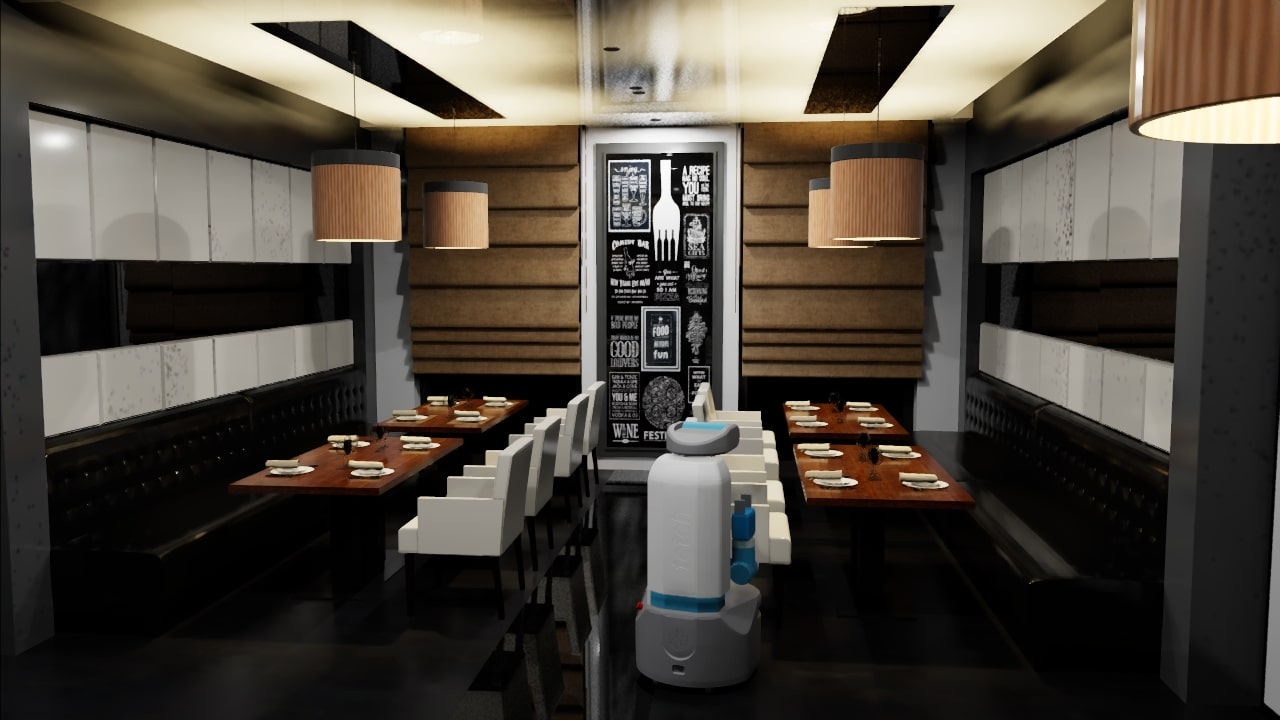
\includegraphics[width=\textwidth]{figures/omnigibson/robot_images/third_pov.jpg}}%
\caption*{\scriptsize3rd Person View}%
\end{subfigure}%
\hfill%
%\subfloat[][\scriptsize RGB]
\begin{subfigure}[t]{0.17\textwidth}{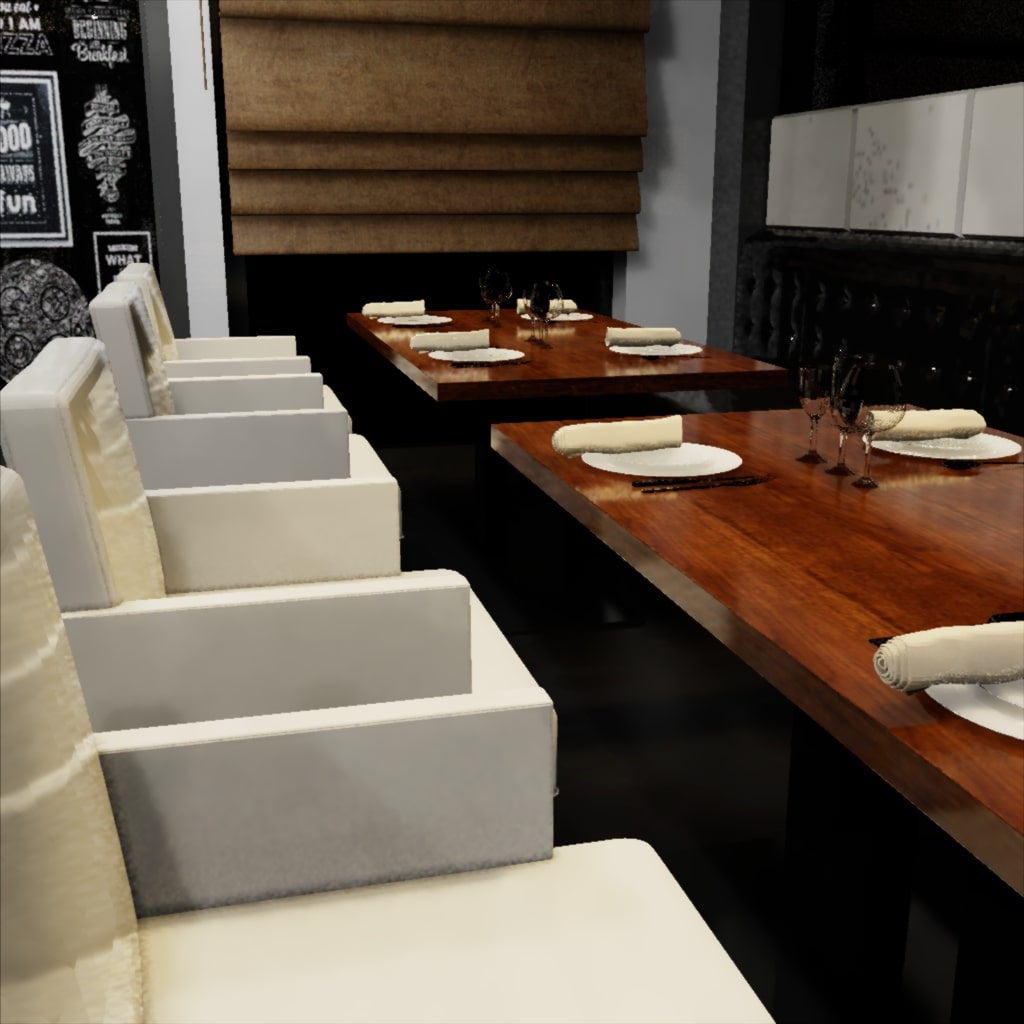
\includegraphics[width=\textwidth]{figures/omnigibson/robot_images/rgb.jpg}}%
\caption*{\scriptsize RGB}%
\end{subfigure}%
\hfill%
%\subfloat[][\scriptsize Depth]
\begin{subfigure}[t]{0.17\textwidth}{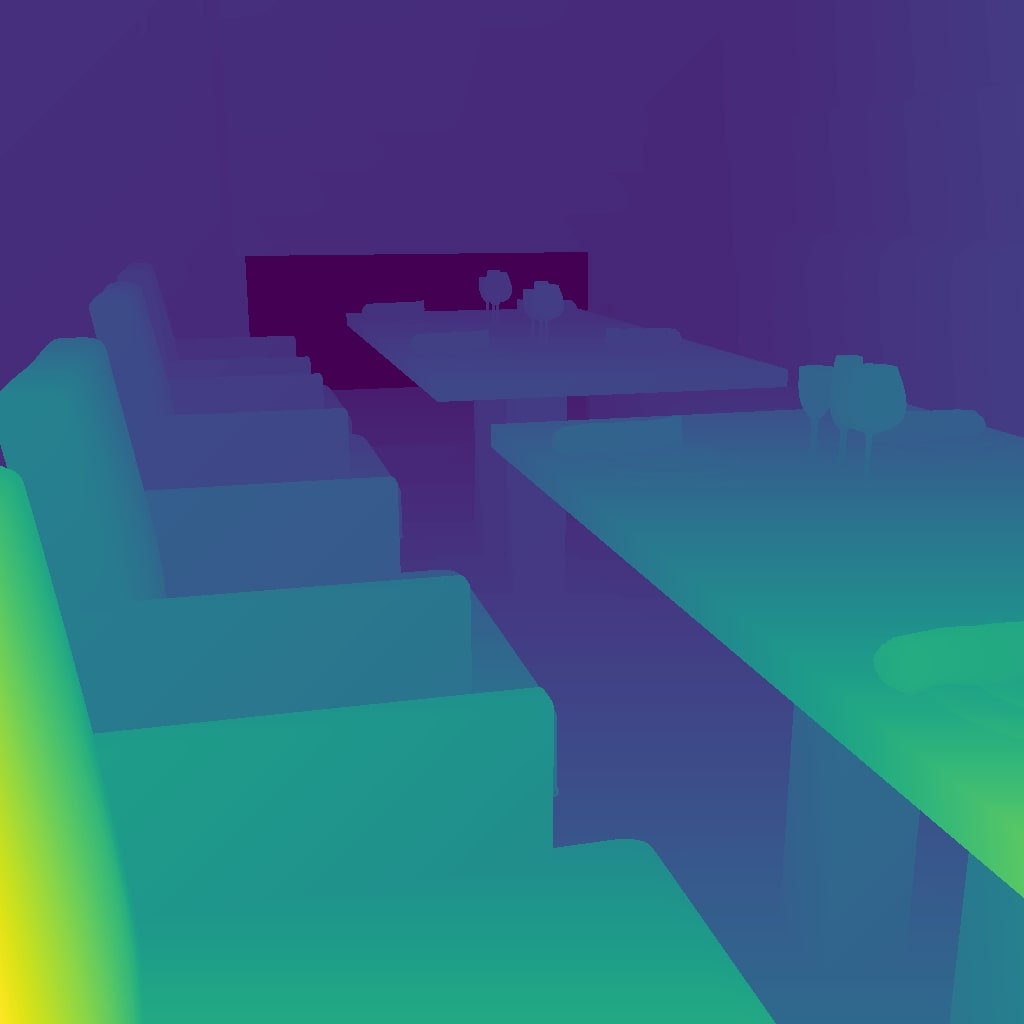
\includegraphics[width=\textwidth]{figures/omnigibson/robot_images/depth.jpg}}%
\caption*{\scriptsize Depth}%
\end{subfigure}%
\hfill%
%\subfloat[][\scriptsize Normals]
\begin{subfigure}[t]{0.17\textwidth}{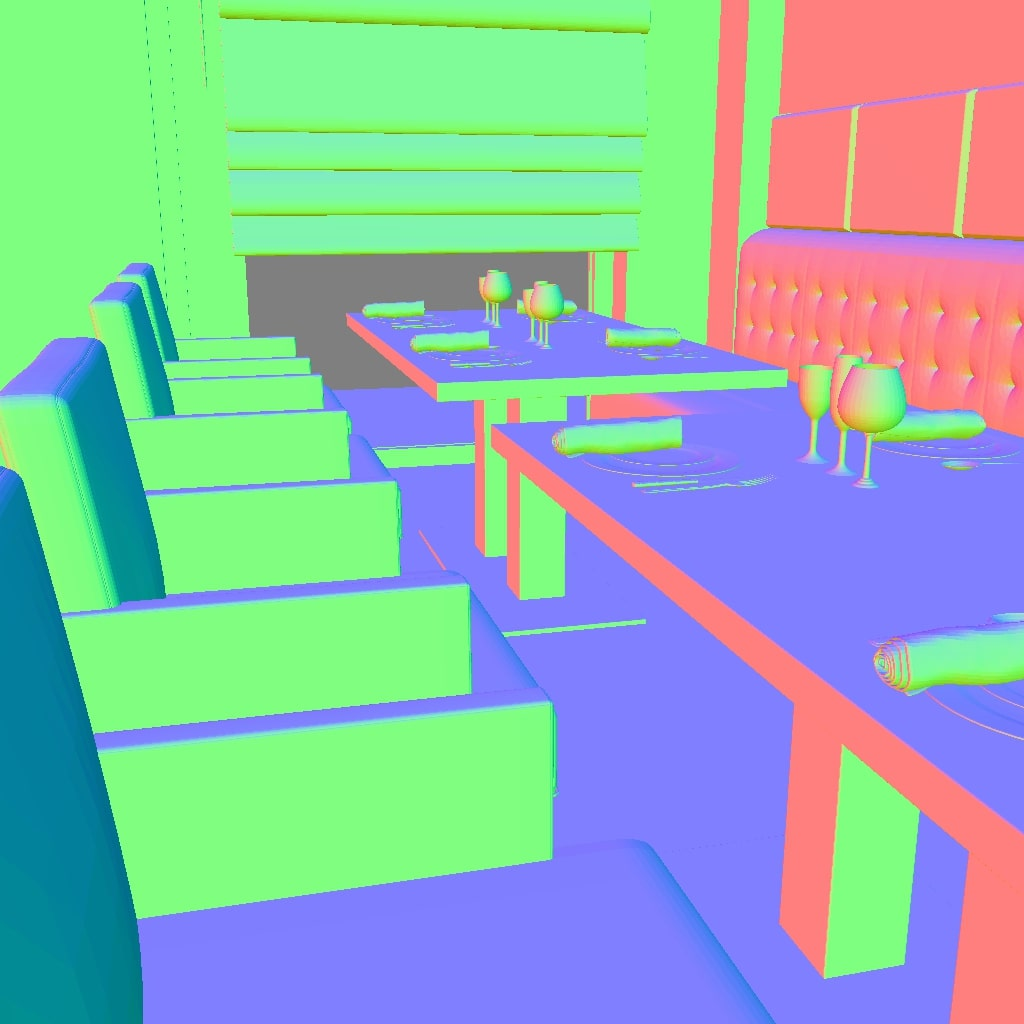
\includegraphics[width=\textwidth]{figures/omnigibson/robot_images/normal.jpg}}%
\caption*{\scriptsize Normals}%
\end{subfigure}%
\hfill%
% \subfloat[][\scriptsize Inst. Segm.]
\begin{subfigure}[t]{0.17\textwidth}{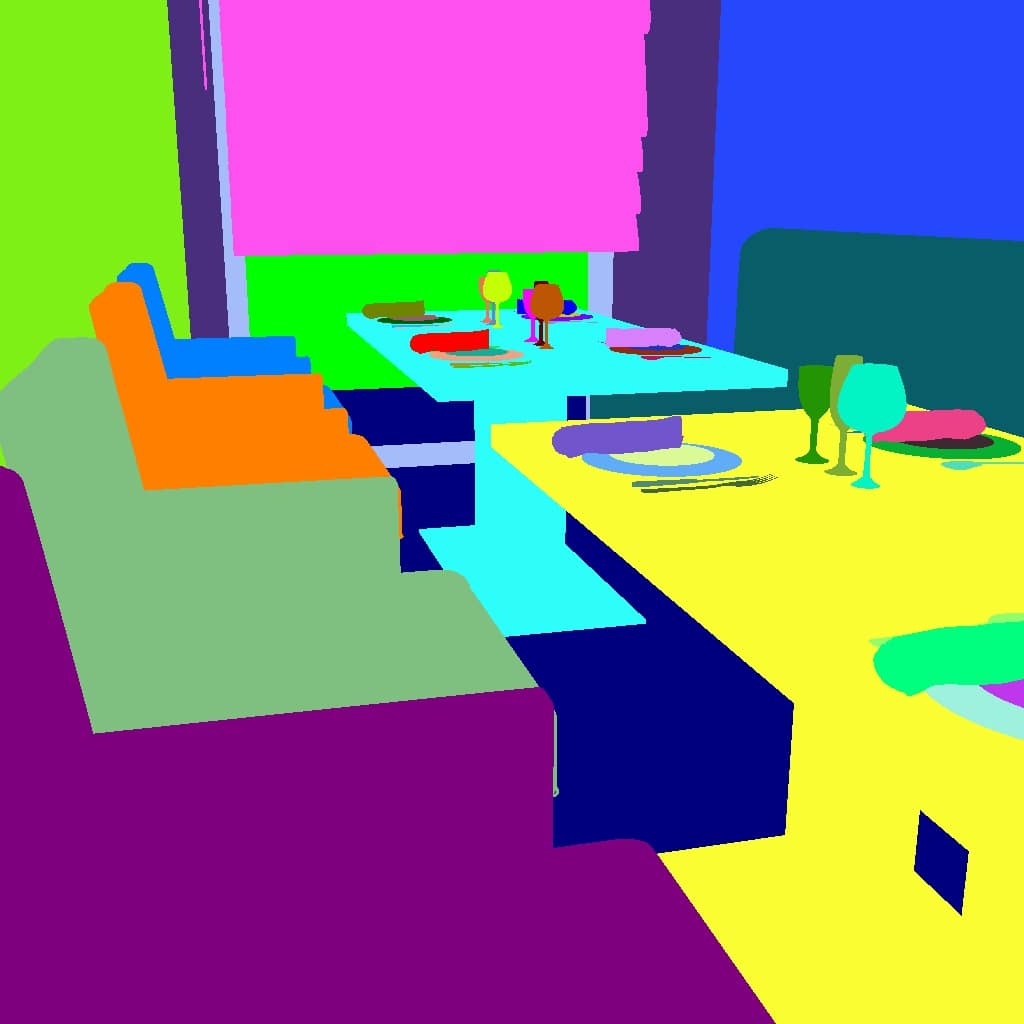
\includegraphics[width=\textwidth]{figures/omnigibson/robot_images/seg_instance.jpg}}%
\caption*{\scriptsize Inst. Segm.}%
\end{subfigure}%
\captionsetup[figure]{font=small,skip=-2pt}%
\caption{\textbf{Visual modalities provided by \simulator.} The robot observes the scene (left, 3rd person view) and obtains visual observations from its onboard sensors including RGB images, depth, normals, and instance segmentation. Rendered RGB images are highly realistic, and, combined with the diverse set of visual observations, can be used to train visual policies.}
\label{fig:sim_modalities}
\end{figure}

% 
\begin{figure}[t]
\captionsetup[subfloat]{labelformat=empty}
\captionsetup[subfloat]{justification=centering}
\centering

\subfloat[\simulator]{}
\hfill
\subfloat[][AI2-Thor]{}
\hfill
\subfloat[][ThreeDWorld]{}
\hfill
\subfloat[][Habitat 2.0]{}
\hfill
\subfloat[][iGibson 2.0]{}

\subfloat[][]{\includegraphics[width=.199\textwidth]{figures/omnigibson/amt_study/og/1.jpg}}
\hfill
\subfloat[][]{\includegraphics[width=.199\textwidth]{figures/omnigibson/amt_study/ai2/1.jpg}}
\hfill
\subfloat[][]{\includegraphics[width=.199\textwidth]{figures/omnigibson/amt_study/tdw/1.jpg}}
\hfill
\subfloat[][]{\includegraphics[width=.199\textwidth]{figures/omnigibson/amt_study/habitat/1.jpg}}
\hfill
\subfloat[][]{\includegraphics[width=.199\textwidth]{figures/omnigibson/amt_study/ig2/1.jpg}}

\vspace{-6pt}

\subfloat[][]{\includegraphics[width=.199\textwidth]{figures/omnigibson/amt_study/og/2.jpg}}
\hfill
\subfloat[][]{\includegraphics[width=.199\textwidth]{figures/omnigibson/amt_study/ai2/2.jpg}}
\hfill
\subfloat[][]{\includegraphics[width=.199\textwidth]{figures/omnigibson/amt_study/tdw/2.jpg}}
\hfill
\subfloat[][]{\includegraphics[width=.199\textwidth]{figures/omnigibson/amt_study/habitat/2.jpg}}
\hfill
\subfloat[][]{\includegraphics[width=.199\textwidth]{figures/omnigibson/amt_study/ig2/2.jpg}}

\vspace{-6pt}

\subfloat[][]{\includegraphics[width=.199\textwidth]{figures/omnigibson/amt_study/og/3.jpg}}
\hfill
\subfloat[][]{\includegraphics[width=.199\textwidth]{figures/omnigibson/amt_study/ai2/3.jpg}}
\hfill
\subfloat[][]{\includegraphics[width=.199\textwidth]{figures/omnigibson/amt_study/tdw/3.jpg}}
\hfill
\subfloat[][]{\includegraphics[width=.199\textwidth]{figures/omnigibson/amt_study/habitat/3.jpg}}
\hfill
\subfloat[][]{\includegraphics[width=.199\textwidth]{figures/omnigibson/amt_study/ig2/3.jpg}}

\vspace{-6pt}

\subfloat[][]{\includegraphics[width=.199\textwidth]{figures/omnigibson/amt_study/og/4.jpg}}
\hfill
\subfloat[][]{\includegraphics[width=.199\textwidth]{figures/omnigibson/amt_study/ai2/4.jpg}}
\hfill
\subfloat[][]{\includegraphics[width=.199\textwidth]{figures/omnigibson/amt_study/tdw/4.jpg}}
\hfill
\subfloat[][]{\includegraphics[width=.199\textwidth]{figures/omnigibson/amt_study/habitat/4.jpg}}
\hfill
\subfloat[][]{\includegraphics[width=.199\textwidth]{figures/omnigibson/amt_study/ig2/4.jpg}}

\vspace{-6pt}

\subfloat[][]{\includegraphics[width=.199\textwidth]{figures/omnigibson/amt_study/og/5.jpg}}
\hfill
\subfloat[][]{\includegraphics[width=.199\textwidth]{figures/omnigibson/amt_study/ai2/5.jpg}}
\hfill
\subfloat[][]{\includegraphics[width=.199\textwidth]{figures/omnigibson/amt_study/tdw/5.jpg}}
\hfill
\subfloat[][]{\includegraphics[width=.199\textwidth]{figures/omnigibson/amt_study/habitat/5.jpg}}
\hfill
\subfloat[][]{\includegraphics[width=.199\textwidth]{figures/omnigibson/amt_study/ig2/5.jpg}}

\vspace{-6pt}

\subfloat[][]{\includegraphics[width=.199\textwidth]{figures/omnigibson/amt_study/og/6.jpg}}
\hfill
\subfloat[][]{\includegraphics[width=.199\textwidth]{figures/omnigibson/amt_study/ai2/6.jpg}}
\hfill
\subfloat[][]{\includegraphics[width=.199\textwidth]{figures/omnigibson/amt_study/tdw/6.jpg}}
\hfill
\subfloat[][]{\includegraphics[width=.199\textwidth]{figures/omnigibson/amt_study/habitat/6.jpg}}
\hfill
\subfloat[][]{\includegraphics[width=.199\textwidth]{figures/omnigibson/amt_study/ig2/6.jpg}}

\vspace{-6pt}

\subfloat[][]{\includegraphics[width=.199\textwidth]{figures/omnigibson/amt_study/og/7.jpg}}
\hfill
\subfloat[][]{\includegraphics[width=.199\textwidth]{figures/omnigibson/amt_study/ai2/7.jpg}}
\hfill
\subfloat[][]{\includegraphics[width=.199\textwidth]{figures/omnigibson/amt_study/tdw/7.jpg}}
\hfill
\subfloat[][]{\includegraphics[width=.199\textwidth]{figures/omnigibson/amt_study/habitat/7.jpg}}
\hfill
\subfloat[][]{\includegraphics[width=.199\textwidth]{figures/omnigibson/amt_study/ig2/7.jpg}}

\vspace{-6pt}

\subfloat[][]{\includegraphics[width=.199\textwidth]{figures/omnigibson/amt_study/og/8.jpg}}
\hfill
\subfloat[][]{\includegraphics[width=.199\textwidth]{figures/omnigibson/amt_study/ai2/8.jpg}}
\hfill
\subfloat[][]{\includegraphics[width=.199\textwidth]{figures/omnigibson/amt_study/tdw/8.jpg}}
\hfill
\subfloat[][]{\includegraphics[width=.199\textwidth]{figures/omnigibson/amt_study/habitat/8.jpg}}
\hfill
\subfloat[][]{\includegraphics[width=.199\textwidth]{figures/omnigibson/amt_study/ig2/8.jpg}}

\vspace{-6pt}

\subfloat[][]{\includegraphics[width=.199\textwidth]{figures/omnigibson/amt_study/og/9.jpg}}
\hfill
\subfloat[][]{\includegraphics[width=.199\textwidth]{figures/omnigibson/amt_study/ai2/9.jpg}}
\hfill
\subfloat[][]{\includegraphics[width=.199\textwidth]{figures/omnigibson/amt_study/tdw/9.jpg}}
\hfill
\subfloat[][]{\includegraphics[width=.199\textwidth]{figures/omnigibson/amt_study/habitat/9.jpg}}
\hfill
\subfloat[][]{\includegraphics[width=.199\textwidth]{figures/omnigibson/amt_study/ig2/9.jpg}}

\vspace{-6pt}

\subfloat[][]{\includegraphics[width=.199\textwidth]{figures/omnigibson/amt_study/og/10.jpg}}
\hfill
\subfloat[][]{\includegraphics[width=.199\textwidth]{figures/omnigibson/amt_study/ai2/10.jpg}}
\hfill
\subfloat[][]{\includegraphics[width=.199\textwidth]{figures/omnigibson/amt_study/tdw/10.jpg}}
\hfill
\subfloat[][]{\includegraphics[width=.199\textwidth]{figures/omnigibson/amt_study/habitat/10.jpg}}
\hfill
\subfloat[][]{\includegraphics[width=.199\textwidth]{figures/omnigibson/amt_study/ig2/10.jpg}}

\vspace{-6pt}

\subfloat[][]{\includegraphics[width=.199\textwidth]{figures/omnigibson/amt_study/og/11.jpg}}
\hfill
\subfloat[][]{\includegraphics[width=.199\textwidth]{figures/omnigibson/amt_study/ai2/11.jpg}}
\hfill
\subfloat[][]{\includegraphics[width=.199\textwidth]{figures/omnigibson/amt_study/tdw/11.jpg}}
\hfill
\subfloat[][]{\includegraphics[width=.199\textwidth]{figures/omnigibson/amt_study/habitat/11.jpg}}
\hfill
\subfloat[][]{\includegraphics[width=.199\textwidth]{figures/omnigibson/amt_study/ig2/11.jpg}}

\vspace{-6pt}

\subfloat[][]{\includegraphics[width=.199\textwidth]{figures/omnigibson/amt_study/og/12.jpg}}
\hfill
\subfloat[][]{\includegraphics[width=.199\textwidth]{figures/omnigibson/amt_study/ai2/12.jpg}}
\hfill
\subfloat[][]{\includegraphics[width=.199\textwidth]{figures/omnigibson/amt_study/tdw/12.jpg}}
\hfill
\subfloat[][]{\includegraphics[width=.199\textwidth]{figures/omnigibson/amt_study/habitat/12.jpg}}
\hfill
\subfloat[][]{\includegraphics[width=.199\textwidth]{figures/omnigibson/amt_study/ig2/12.jpg}}

\vspace{-6pt}

\subfloat[][]{\includegraphics[width=.199\textwidth]{figures/omnigibson/amt_study/og/13.jpg}}
\hfill
\subfloat[][]{\includegraphics[width=.199\textwidth]{figures/omnigibson/amt_study/ai2/13.jpg}}
\hfill
\subfloat[][]{\includegraphics[width=.199\textwidth]{figures/omnigibson/amt_study/tdw/13.jpg}}
\hfill
\subfloat[][]{\includegraphics[width=.199\textwidth]{figures/omnigibson/amt_study/habitat/13.jpg}}
\hfill
\subfloat[][]{\includegraphics[width=.199\textwidth]{figures/omnigibson/amt_study/ig2/13.jpg}}

\end{figure}
% \vspace{-6pt}

\begin{figure}[t]
\captionsetup[subfloat]{labelformat=empty}
\captionsetup[subfloat]{justification=centering}
\centering
% \ContinuedFloat

\subfloat[][]{\includegraphics[width=.199\textwidth]{figures/omnigibson/amt_study/og/14.jpg}}
\hfill
\subfloat[][]{\includegraphics[width=.199\textwidth]{figures/omnigibson/amt_study/ai2/14.jpg}}
\hfill
\subfloat[][]{\includegraphics[width=.199\textwidth]{figures/omnigibson/amt_study/tdw/14.jpg}}
\hfill
\subfloat[][]{\includegraphics[width=.199\textwidth]{figures/omnigibson/amt_study/habitat/14.jpg}}
\hfill
\subfloat[][]{\includegraphics[width=.199\textwidth]{figures/omnigibson/amt_study/ig2/14.jpg}}

\vspace{-6pt}

\subfloat[][]{\includegraphics[width=.199\textwidth]{figures/omnigibson/amt_study/og/15.jpg}}
\hfill
\subfloat[][]{\includegraphics[width=.199\textwidth]{figures/omnigibson/amt_study/ai2/15.jpg}}
\hfill
\subfloat[][]{\includegraphics[width=.199\textwidth]{figures/omnigibson/amt_study/tdw/15.jpg}}
\hfill
\subfloat[][]{\includegraphics[width=.199\textwidth]{figures/omnigibson/amt_study/habitat/15.jpg}}
\hfill
\subfloat[][]{\includegraphics[width=.199\textwidth]{figures/omnigibson/amt_study/ig2/15.jpg}}

\vspace{-6pt}

\subfloat[][]{\includegraphics[width=.199\textwidth]{figures/omnigibson/amt_study/og/16.jpg}}
\hfill
\subfloat[][]{\includegraphics[width=.199\textwidth]{figures/omnigibson/amt_study/ai2/16.jpg}}
\hfill
\subfloat[][]{\includegraphics[width=.199\textwidth]{figures/omnigibson/amt_study/tdw/16.jpg}}
\hfill
\subfloat[][]{\includegraphics[width=.199\textwidth]{figures/omnigibson/amt_study/habitat/16.jpg}}
\hfill
\subfloat[][]{\includegraphics[width=.199\textwidth]{figures/omnigibson/amt_study/ig2/16.jpg}}

\vspace{-6pt}

\subfloat[][]{\includegraphics[width=.199\textwidth]{figures/omnigibson/amt_study/og/17.jpg}}
\hfill
\subfloat[][]{\includegraphics[width=.199\textwidth]{figures/omnigibson/amt_study/ai2/17.jpg}}
\hfill
\subfloat[][]{\includegraphics[width=.199\textwidth]{figures/omnigibson/amt_study/tdw/17.jpg}}
\hfill
\subfloat[][]{\includegraphics[width=.199\textwidth]{figures/omnigibson/amt_study/habitat/17.jpg}}
\hfill
\subfloat[][]{\includegraphics[width=.199\textwidth]{figures/omnigibson/amt_study/ig2/17.jpg}}

\vspace{-6pt}

\subfloat[][]{\includegraphics[width=.199\textwidth]{figures/omnigibson/amt_study/og/18.jpg}}
\hfill
\subfloat[][]{\includegraphics[width=.199\textwidth]{figures/omnigibson/amt_study/ai2/18.jpg}}
\hfill
\subfloat[][]{\includegraphics[width=.199\textwidth]{figures/omnigibson/amt_study/tdw/18.jpg}}
\hfill
\subfloat[][]{\includegraphics[width=.199\textwidth]{figures/omnigibson/amt_study/habitat/18.jpg}}
\hfill
\subfloat[][]{\includegraphics[width=.199\textwidth]{figures/omnigibson/amt_study/ig2/18.jpg}}

\vspace{-6pt}

\subfloat[][]{\includegraphics[width=.199\textwidth]{figures/omnigibson/amt_study/og/19.jpg}}
\hfill
\subfloat[][]{\includegraphics[width=.199\textwidth]{figures/omnigibson/amt_study/ai2/19.jpg}}
\hfill
\subfloat[][]{\includegraphics[width=.199\textwidth]{figures/omnigibson/amt_study/tdw/19.jpg}}
\hfill
\subfloat[][]{\includegraphics[width=.199\textwidth]{figures/omnigibson/amt_study/habitat/19.jpg}}
\hfill
\subfloat[][]{\includegraphics[width=.199\textwidth]{figures/omnigibson/amt_study/ig2/19.jpg}}

\vspace{-6pt}

\subfloat[][]{\includegraphics[width=.199\textwidth]{figures/omnigibson/amt_study/og/20.jpg}}
\hfill
\subfloat[][]{\includegraphics[width=.199\textwidth]{figures/omnigibson/amt_study/ai2/20.jpg}}
\hfill
\subfloat[][]{\includegraphics[width=.199\textwidth]{figures/omnigibson/amt_study/tdw/20.jpg}}
\hfill
\subfloat[][]{\includegraphics[width=.199\textwidth]{figures/omnigibson/amt_study/habitat/20.jpg}}
\hfill
\subfloat[][]{\includegraphics[width=.199\textwidth]{figures/omnigibson/amt_study/ig2/20.jpg}}

\vspace{-6pt}

\subfloat[][]{\includegraphics[width=.199\textwidth]{figures/omnigibson/amt_study/og/21.jpg}}
\hfill
\subfloat[][]{\includegraphics[width=.199\textwidth]{figures/omnigibson/amt_study/ai2/21.jpg}}
\hfill
\subfloat[][]{\includegraphics[width=.199\textwidth]{figures/omnigibson/amt_study/tdw/21.jpg}}
\hfill
\subfloat[][]{\includegraphics[width=.199\textwidth]{figures/omnigibson/amt_study/habitat/21.jpg}}
\hfill
\subfloat[][]{\includegraphics[width=.199\textwidth]{figures/omnigibson/amt_study/ig2/21.jpg}}

\vspace{-6pt}

\subfloat[][]{\includegraphics[width=.199\textwidth]{figures/omnigibson/amt_study/og/22.jpg}}
\hfill
\subfloat[][]{\includegraphics[width=.199\textwidth]{figures/omnigibson/amt_study/ai2/22.jpg}}
\hfill
\subfloat[][]{\includegraphics[width=.199\textwidth]{figures/omnigibson/amt_study/tdw/22.jpg}}
\hfill
\subfloat[][]{\includegraphics[width=.199\textwidth]{figures/omnigibson/amt_study/habitat/22.jpg}}
\hfill
\subfloat[][]{\includegraphics[width=.199\textwidth]{figures/omnigibson/amt_study/ig2/22.jpg}}

\vspace{-6pt}

\subfloat[][]{\includegraphics[width=.199\textwidth]{figures/omnigibson/amt_study/og/23.jpg}}
\hfill
\subfloat[][]{\includegraphics[width=.199\textwidth]{figures/omnigibson/amt_study/ai2/23.jpg}}
\hfill
\subfloat[][]{\includegraphics[width=.199\textwidth]{figures/omnigibson/amt_study/tdw/23.jpg}}
\hfill
\subfloat[][]{\includegraphics[width=.199\textwidth]{figures/omnigibson/amt_study/habitat/23.jpg}}
\hfill
\subfloat[][]{\includegraphics[width=.199\textwidth]{figures/omnigibson/amt_study/ig2/23.jpg}}

\vspace{-6pt}

\subfloat[][]{\includegraphics[width=.199\textwidth]{figures/omnigibson/amt_study/og/24.jpg}}
\hfill
\subfloat[][]{\includegraphics[width=.199\textwidth]{figures/omnigibson/amt_study/ai2/24.jpg}}
\hfill
\subfloat[][]{\includegraphics[width=.199\textwidth]{figures/omnigibson/amt_study/tdw/24.jpg}}
\hfill
\subfloat[][]{\includegraphics[width=.199\textwidth]{figures/omnigibson/amt_study/habitat/24.jpg}}
\hfill
\subfloat[][]{\includegraphics[width=.199\textwidth]{figures/omnigibson/amt_study/ig2/24.jpg}}

\vspace{-6pt}

\subfloat[][]{\includegraphics[width=.199\textwidth]{figures/omnigibson/amt_study/og/25.jpg}}
\hfill
\subfloat[][]{\includegraphics[width=.199\textwidth]{figures/omnigibson/amt_study/ai2/25.jpg}}
\hfill
\subfloat[][]{\includegraphics[width=.199\textwidth]{figures/omnigibson/amt_study/tdw/25.jpg}}
\hfill
\subfloat[][]{\includegraphics[width=.199\textwidth]{figures/omnigibson/amt_study/habitat/25.jpg}}
\hfill
\subfloat[][]{\includegraphics[width=.199\textwidth]{figures/omnigibson/amt_study/ig2/25.jpg}}

\vspace{-6pt}

\subfloat[][]{\includegraphics[width=.199\textwidth]{figures/omnigibson/amt_study/og/26.jpg}}
\hfill
\subfloat[][]{\includegraphics[width=.199\textwidth]{figures/omnigibson/amt_study/ai2/26.jpg}}
\hfill
\subfloat[][]{\includegraphics[width=.199\textwidth]{figures/omnigibson/amt_study/tdw/26.jpg}}
\hfill
\subfloat[][]{\includegraphics[width=.199\textwidth]{figures/omnigibson/amt_study/habitat/26.jpg}}
\hfill
\subfloat[][]{\includegraphics[width=.199\textwidth]{figures/omnigibson/amt_study/ig2/26.jpg}}

\end{figure}
% \vspace{-6pt}

\begin{figure}[t]
\captionsetup[subfloat]{labelformat=empty}
\captionsetup[subfloat]{justification=centering}
\centering

\subfloat[][]{\includegraphics[width=.199\textwidth]{figures/omnigibson/amt_study/og/27.jpg}}
\hfill
\subfloat[][]{\includegraphics[width=.199\textwidth]{figures/omnigibson/amt_study/ai2/27.jpg}}
\hfill
\subfloat[][]{\includegraphics[width=.199\textwidth]{figures/omnigibson/amt_study/tdw/27.jpg}}
\hfill
\subfloat[][]{\includegraphics[width=.199\textwidth]{figures/omnigibson/amt_study/habitat/27.jpg}}
\hfill
\subfloat[][]{\includegraphics[width=.199\textwidth]{figures/omnigibson/amt_study/ig2/27.jpg}}

\vspace{-6pt}

\subfloat[][]{\includegraphics[width=.199\textwidth]{figures/omnigibson/amt_study/og/28.jpg}}
\hfill
\subfloat[][]{\includegraphics[width=.199\textwidth]{figures/omnigibson/amt_study/ai2/28.jpg}}
\hfill
\subfloat[][]{\includegraphics[width=.199\textwidth]{figures/omnigibson/amt_study/tdw/28.jpg}}
\hfill
\subfloat[][]{\includegraphics[width=.199\textwidth]{figures/omnigibson/amt_study/habitat/28.jpg}}
\hfill
\subfloat[][]{\includegraphics[width=.199\textwidth]{figures/omnigibson/amt_study/ig2/28.jpg}}

\vspace{-6pt}

\subfloat[][]{\includegraphics[width=.199\textwidth]{figures/omnigibson/amt_study/og/29.jpg}}
\hfill
\subfloat[][]{\includegraphics[width=.199\textwidth]{figures/omnigibson/amt_study/ai2/29.jpg}}
\hfill
\subfloat[][]{\includegraphics[width=.199\textwidth]{figures/omnigibson/amt_study/tdw/29.jpg}}
\hfill
\subfloat[][]{\includegraphics[width=.199\textwidth]{figures/omnigibson/amt_study/habitat/29.jpg}}
\hfill
\subfloat[][]{\includegraphics[width=.199\textwidth]{figures/omnigibson/amt_study/ig2/29.jpg}}

\vspace{-6pt}

\subfloat[][]{\includegraphics[width=.199\textwidth]{figures/omnigibson/amt_study/og/30.jpg}}
\hfill
\subfloat[][]{\includegraphics[width=.199\textwidth]{figures/omnigibson/amt_study/ai2/30.jpg}}
\hfill
\subfloat[][]{\includegraphics[width=.199\textwidth]{figures/omnigibson/amt_study/tdw/30.jpg}}
\hfill
\subfloat[][]{\includegraphics[width=.199\textwidth]{figures/omnigibson/amt_study/habitat/30.jpg}}
\hfill
\subfloat[][]{\includegraphics[width=.199\textwidth]{figures/omnigibson/amt_study/ig2/30.jpg}}

\vspace{-6pt}

\subfloat[][]{\includegraphics[width=.199\textwidth]{figures/omnigibson/amt_study/og/31.jpg}}
\hfill
\subfloat[][]{\includegraphics[width=.199\textwidth]{figures/omnigibson/amt_study/ai2/31.jpg}}
\hfill
\subfloat[][]{\includegraphics[width=.199\textwidth]{figures/omnigibson/amt_study/tdw/31.jpg}}
\hfill
\subfloat[][]{\includegraphics[width=.199\textwidth]{figures/omnigibson/amt_study/habitat/31.jpg}}
\hfill
\subfloat[][]{\includegraphics[width=.199\textwidth]{figures/omnigibson/amt_study/ig2/31.jpg}}

\vspace{-6pt}

\subfloat[][]{\includegraphics[width=.199\textwidth]{figures/omnigibson/amt_study/og/32.jpg}}
\hfill
\subfloat[][]{\includegraphics[width=.199\textwidth]{figures/omnigibson/amt_study/ai2/32.jpg}}
\hfill
\subfloat[][]{\includegraphics[width=.199\textwidth]{figures/omnigibson/amt_study/tdw/32.jpg}}
\hfill
\subfloat[][]{\includegraphics[width=.199\textwidth]{figures/omnigibson/amt_study/habitat/32.jpg}}
\hfill
\subfloat[][]{\includegraphics[width=.199\textwidth]{figures/omnigibson/amt_study/ig2/32.jpg}}

\vspace{-6pt}

\subfloat[][]{\includegraphics[width=.199\textwidth]{figures/omnigibson/amt_study/og/33.jpg}}
\hfill
\subfloat[][]{\includegraphics[width=.199\textwidth]{figures/omnigibson/amt_study/ai2/33.jpg}}
\hfill
\subfloat[][]{\includegraphics[width=.199\textwidth]{figures/omnigibson/amt_study/tdw/33.jpg}}
\hfill
\subfloat[][]{\includegraphics[width=.199\textwidth]{figures/omnigibson/amt_study/habitat/33.jpg}}
\hfill
\subfloat[][]{\includegraphics[width=.199\textwidth]{figures/omnigibson/amt_study/ig2/33.jpg}}

\vspace{-6pt}

\subfloat[][]{\includegraphics[width=.199\textwidth]{figures/omnigibson/amt_study/og/34.jpg}}
\hfill
\subfloat[][]{\includegraphics[width=.199\textwidth]{figures/omnigibson/amt_study/ai2/34.jpg}}
\hfill
\subfloat[][]{\includegraphics[width=.199\textwidth]{figures/omnigibson/amt_study/tdw/34.jpg}}
\hfill
\subfloat[][]{\includegraphics[width=.199\textwidth]{figures/omnigibson/amt_study/habitat/34.jpg}}
\hfill
\subfloat[][]{\includegraphics[width=.199\textwidth]{figures/omnigibson/amt_study/ig2/34.jpg}}

\vspace{-6pt}

\subfloat[][]{\includegraphics[width=.199\textwidth]{figures/omnigibson/amt_study/og/35.jpg}}
\hfill
\subfloat[][]{\includegraphics[width=.199\textwidth]{figures/omnigibson/amt_study/ai2/35.jpg}}
\hfill
\subfloat[][]{\includegraphics[width=.199\textwidth]{figures/omnigibson/amt_study/tdw/35.jpg}}
\hfill
\subfloat[][]{\includegraphics[width=.199\textwidth]{figures/omnigibson/amt_study/habitat/35.jpg}}
\hfill
\subfloat[][]{\includegraphics[width=.199\textwidth]{figures/omnigibson/amt_study/ig2/35.jpg}}

\vspace{-6pt}

\subfloat[][]{\includegraphics[width=.199\textwidth]{figures/omnigibson/amt_study/og/36.jpg}}
\hfill
\subfloat[][]{\includegraphics[width=.199\textwidth]{figures/omnigibson/amt_study/ai2/36.jpg}}
\hfill
\subfloat[][]{\includegraphics[width=.199\textwidth]{figures/omnigibson/amt_study/tdw/36.jpg}}
\hfill
\subfloat[][]{\includegraphics[width=.199\textwidth]{figures/omnigibson/amt_study/habitat/36.jpg}}
\hfill
\subfloat[][]{\includegraphics[width=.199\textwidth]{figures/omnigibson/amt_study/ig2/36.jpg}}

\vspace{-6pt}

\subfloat[][]{\includegraphics[width=.199\textwidth]{figures/omnigibson/amt_study/og/37.jpg}}
\hfill
\subfloat[][]{\includegraphics[width=.199\textwidth]{figures/omnigibson/amt_study/ai2/37.jpg}}
\hfill
\subfloat[][]{\includegraphics[width=.199\textwidth]{figures/omnigibson/amt_study/tdw/37.jpg}}
\hfill
\subfloat[][]{\includegraphics[width=.199\textwidth]{figures/omnigibson/amt_study/habitat/37.jpg}}
\hfill
\subfloat[][]{\includegraphics[width=.199\textwidth]{figures/omnigibson/amt_study/ig2/37.jpg}}

\vspace{-6pt}

\subfloat[][]{\includegraphics[width=.199\textwidth]{figures/omnigibson/amt_study/og/38.jpg}}
\hfill
\subfloat[][]{\includegraphics[width=.199\textwidth]{figures/omnigibson/amt_study/ai2/38.jpg}}
\hfill
\subfloat[][]{\includegraphics[width=.199\textwidth]{figures/omnigibson/amt_study/tdw/38.jpg}}
\hfill
\subfloat[][]{\includegraphics[width=.199\textwidth]{figures/omnigibson/amt_study/habitat/38.jpg}}
\hfill
\subfloat[][]{\includegraphics[width=.199\textwidth]{figures/omnigibson/amt_study/ig2/38.jpg}}

\vspace{-6pt}

\subfloat[][]{\includegraphics[width=.199\textwidth]{figures/omnigibson/amt_study/og/39.jpg}}
\hfill
\subfloat[][]{\includegraphics[width=.199\textwidth]{figures/omnigibson/amt_study/ai2/39.jpg}}
\hfill
\subfloat[][]{\includegraphics[width=.199\textwidth]{figures/omnigibson/amt_study/tdw/39.jpg}}
\hfill
\subfloat[][]{\includegraphics[width=.199\textwidth]{figures/omnigibson/amt_study/habitat/39.jpg}}
\hfill
\subfloat[][]{\includegraphics[width=.199\textwidth]{figures/omnigibson/amt_study/ig2/39.jpg}}

\end{figure}
% \vspace{-6pt}

\begin{figure}[t]
\captionsetup[subfloat]{labelformat=empty}
\captionsetup[subfloat]{justification=centering}
\centering

\subfloat[][]{\includegraphics[width=.199\textwidth]{figures/omnigibson/amt_study/og/40.jpg}}
\hfill
\subfloat[][]{\includegraphics[width=.199\textwidth]{figures/omnigibson/amt_study/ai2/40.jpg}}
\hfill
\subfloat[][]{\includegraphics[width=.199\textwidth]{figures/omnigibson/amt_study/tdw/40.jpg}}
\hfill
\subfloat[][]{\includegraphics[width=.199\textwidth]{figures/omnigibson/amt_study/habitat/40.jpg}}
\hfill
\subfloat[][]{\includegraphics[width=.199\textwidth]{figures/omnigibson/amt_study/ig2/40.jpg}}

\vspace{-6pt}

\subfloat[][]{\includegraphics[width=.199\textwidth]{figures/omnigibson/amt_study/og/41.jpg}}
\hfill
\subfloat[][]{\includegraphics[width=.199\textwidth]{figures/omnigibson/amt_study/ai2/41.jpg}}
\hfill
\subfloat[][]{\includegraphics[width=.199\textwidth]{figures/omnigibson/amt_study/tdw/41.jpg}}
\hfill
\subfloat[][]{\includegraphics[width=.199\textwidth]{figures/omnigibson/amt_study/habitat/41.jpg}}
\hfill
\subfloat[][]{\includegraphics[width=.199\textwidth]{figures/omnigibson/amt_study/ig2/41.jpg}}

\vspace{-6pt}

\subfloat[][]{\includegraphics[width=.199\textwidth]{figures/omnigibson/amt_study/og/42.jpg}}
\hfill
\subfloat[][]{\includegraphics[width=.199\textwidth]{figures/omnigibson/amt_study/ai2/42.jpg}}
\hfill
\subfloat[][]{\includegraphics[width=.199\textwidth]{figures/omnigibson/amt_study/tdw/42.jpg}}
\hfill
\subfloat[][]{\includegraphics[width=.199\textwidth]{figures/omnigibson/amt_study/habitat/42.jpg}}
\hfill
\subfloat[][]{\includegraphics[width=.199\textwidth]{figures/omnigibson/amt_study/ig2/42.jpg}}

\vspace{-6pt}

\subfloat[][]{\includegraphics[width=.199\textwidth]{figures/omnigibson/amt_study/og/43.jpg}}
\hfill
\subfloat[][]{\includegraphics[width=.199\textwidth]{figures/omnigibson/amt_study/ai2/43.jpg}}
\hfill
\subfloat[][]{\includegraphics[width=.199\textwidth]{figures/omnigibson/amt_study/tdw/43.jpg}}
\hfill
\subfloat[][]{\includegraphics[width=.199\textwidth]{figures/omnigibson/amt_study/habitat/43.jpg}}
\hfill
\subfloat[][]{\includegraphics[width=.199\textwidth]{figures/omnigibson/amt_study/ig2/43.jpg}}

\vspace{-6pt}

\subfloat[][]{\includegraphics[width=.199\textwidth]{figures/omnigibson/amt_study/og/44.jpg}}
\hfill
\subfloat[][]{\includegraphics[width=.199\textwidth]{figures/omnigibson/amt_study/ai2/44.jpg}}
\hfill
\subfloat[][]{\includegraphics[width=.199\textwidth]{figures/omnigibson/amt_study/tdw/44.jpg}}
\hfill
\subfloat[][]{\includegraphics[width=.199\textwidth]{figures/omnigibson/amt_study/habitat/44.jpg}}
\hfill
\subfloat[][]{\includegraphics[width=.199\textwidth]{figures/omnigibson/amt_study/ig2/44.jpg}}

\vspace{-6pt}

\subfloat[][]{\includegraphics[width=.199\textwidth]{figures/omnigibson/amt_study/og/45.jpg}}
\hfill
\subfloat[][]{\includegraphics[width=.199\textwidth]{figures/omnigibson/amt_study/ai2/45.jpg}}
\hfill
\subfloat[][]{\includegraphics[width=.199\textwidth]{figures/omnigibson/amt_study/tdw/45.jpg}}
\hfill
\subfloat[][]{\includegraphics[width=.199\textwidth]{figures/omnigibson/amt_study/habitat/45.jpg}}
\hfill
\subfloat[][]{\includegraphics[width=.199\textwidth]{figures/omnigibson/amt_study/ig2/45.jpg}}

\vspace{-6pt}

\subfloat[][]{\includegraphics[width=.199\textwidth]{figures/omnigibson/amt_study/og/46.jpg}}
\hfill
\subfloat[][]{\includegraphics[width=.199\textwidth]{figures/omnigibson/amt_study/ai2/46.jpg}}
\hfill
\subfloat[][]{\includegraphics[width=.199\textwidth]{figures/omnigibson/amt_study/tdw/46.jpg}}
\hfill
\subfloat[][]{\includegraphics[width=.199\textwidth]{figures/omnigibson/amt_study/habitat/46.jpg}}
\hfill
\subfloat[][]{\includegraphics[width=.199\textwidth]{figures/omnigibson/amt_study/ig2/46.jpg}}

\vspace{-6pt}

\subfloat[][]{\includegraphics[width=.199\textwidth]{figures/omnigibson/amt_study/og/47.jpg}}
\hfill
\subfloat[][]{\includegraphics[width=.199\textwidth]{figures/omnigibson/amt_study/ai2/47.jpg}}
\hfill
\subfloat[][]{\includegraphics[width=.199\textwidth]{figures/omnigibson/amt_study/tdw/47.jpg}}
\hfill
\subfloat[][]{\includegraphics[width=.199\textwidth]{figures/omnigibson/amt_study/habitat/47.jpg}}
\hfill
\subfloat[][]{\includegraphics[width=.199\textwidth]{figures/omnigibson/amt_study/ig2/47.jpg}}

\vspace{-6pt}

\subfloat[][]{\includegraphics[width=.199\textwidth]{figures/omnigibson/amt_study/og/48.jpg}}
\hfill
\subfloat[][]{\includegraphics[width=.199\textwidth]{figures/omnigibson/amt_study/ai2/48.jpg}}
\hfill
\subfloat[][]{\includegraphics[width=.199\textwidth]{figures/omnigibson/amt_study/tdw/48.jpg}}
\hfill
\subfloat[][]{\includegraphics[width=.199\textwidth]{figures/omnigibson/amt_study/habitat/48.jpg}}
\hfill
\subfloat[][]{\includegraphics[width=.199\textwidth]{figures/omnigibson/amt_study/ig2/48.jpg}}

\vspace{-6pt}

\subfloat[][]{\includegraphics[width=.199\textwidth]{figures/omnigibson/amt_study/og/49.jpg}}
\hfill
\subfloat[][]{\includegraphics[width=.199\textwidth]{figures/omnigibson/amt_study/ai2/49.jpg}}
\hfill
\subfloat[][]{\includegraphics[width=.199\textwidth]{figures/omnigibson/amt_study/tdw/49.jpg}}
\hfill
\subfloat[][]{\includegraphics[width=.199\textwidth]{figures/omnigibson/amt_study/habitat/49.jpg}}
\hfill
\subfloat[][]{\includegraphics[width=.199\textwidth]{figures/omnigibson/amt_study/ig2/49.jpg}}

\vspace{-6pt}

\subfloat[][]{\includegraphics[width=.199\textwidth]{figures/omnigibson/amt_study/og/50.jpg}}
\hfill
\subfloat[][]{\includegraphics[width=.199\textwidth]{figures/omnigibson/amt_study/ai2/50.jpg}}
\hfill
\subfloat[][]{\includegraphics[width=.199\textwidth]{figures/omnigibson/amt_study/tdw/50.jpg}}
\hfill
\subfloat[][]{\includegraphics[width=.199\textwidth]{figures/omnigibson/amt_study/habitat/50.jpg}}
\hfill
\subfloat[][]{\includegraphics[width=.199\textwidth]{figures/omnigibson/amt_study/ig2/50.jpg}}



\vspace{15pt}
\caption{\textbf{Comparative Evaluation of Visual Realism:} We evaluate \simulator's visual realism against other simulation environments by running a survey with 50 human participants. We ask them to rank the realism of sampled images from each environment with a score of 5 (most realistic) to 1 (least realistic). We report the mean and standard deviation and show a sampled image from the study. We observe that the participants consider \simulator to be significantly more visually realistic than all other environments. See Appendix \ref{amt_study_appx} for more info.}
\label{fig:sim_render}
\end{figure}

\subsection{Visual Modalities}
\simulator provides diverse perceptual modules to capture realistic sensor modalities from an agent's perspective, including RGB, Depth, Semantic Segmentation, Normal, and Optical Flow images, in addition to non-visual modalities such as proprioception and LiDAR scans (Fig.~\ref{fig:sim_modalities}). \simulator also provides varying abstraction levels for agent action spaces, including low-level control, assistive manipulation, and primitive skill execution. Overall, these modules are intended to be useful to the broad embodied AI research community, with the goal of accelerating breakthroughs on \benchmark.

\subsection{Performance Benchmark}

\revision{
To evaluate the performance of \simulator under different conditions, we performed rigorous speed test in two representative scenes (\texttt{Rs\_int} and \texttt{house\_single\_floor}) with different number of objects on a single-GPU, single-process setup. We adopt the ``idle'' setup from \citet{li2021ig2} and \citet{szot2021habitat}: a robot is placed in the scene (except the last row "- Robot"), and stays still with zero velocity action. At each time step, the simulator runs the physics simulation, extended object state update, and transition machine update loop, and renders a $128\times128$ RGB image. We use action time step of $t_a = \frac{1}{60}\text{s}$ and physics time step of $t_s = \frac{1}{60}\text{s}$. Our benchmark runs on a Ubuntu machine with Intel(R) Core(TM) i7-10700K CPU @ 5.10GHz and one Nvidia GeForce RTX 3080 GPU in a single process setting. The results are summarized in Table~\ref{tab:benchmark}.
}

\revision{
\simulator runs at a comparable speed to previous works like iGibson 2.0~\cite{li2021ig2} under similar settings, but with much higher rendering quality thanks to ray-tracing. It maintains a reasonable speed even for a large scene with over 600 objects. \simulator is also highly configurable and provides flexible interface for users to balance between simulation fidelity and speed given their use cases and research interests. If the user isn't interested in fluid or cloth in their tasks, they can turn off these features to harvest performance speedup. Similarly, if the user is only interested in kinematics-only rearrangement tasks, or non-robotics embodied AI applications (e.g. a virtual camera), they can turn off object state update, or remove the robot, respectively. We are actively working on improving aspects that can provide simulation speedups, e.g. in areas like object sleeping, mesh simplification, more efficient object state update. Furthermore, since real-time ray-tracing and fluid/cloth simulation is still an active area of research, we expect the upcoming hardware and software advances from Nvidia will lead to significant performance improvements in these areas.
}

\begin{table}[t]
    \centering
    \begin{tabular}{l|cc}
    \toprule
    \multicolumn{1}{c|}{\multirow{2}{*}{Eval. Conditions}} & \multicolumn{2}{c}{Scene} \\
    \multicolumn{1}{c|}{} & \texttt{Rs\_int} (81 objs) & \texttt{house\_single\_floor} (621 objs) \\ \midrule
    Full Feature Set & $24$ & $11$ \\
    - Fluid and Cloth & $58$ & $26$ \\
    - Object State Update & $77$ & $55$ \\ 
    - Robot & $90$ & $60$ \\ \bottomrule
    \end{tabular}
    \caption{\revision{Benchmarking \simulator performance: simulation steps per second (SPS, higher better) in two representative scenes with 81 and 621 objects, under different evaluation conditions.}}
    \label{tab:benchmark}
\end{table}



% \begin{figure}[t]
%     \centering
%     \includegraphics[width=0.95\textwidth]{figures/omnigibson/Omni_Visual_Modalities.png}
%     \caption{[In appendix] Visualization of visual modalities provided by OmniGibson: RGB images, depth, semantic segmentation, instance segmentation, optical flow, and scene graphs.\fei{would be better from a robot perspective}}
%     \label{fig:sim_modalities}
% \end{figure}


\section{Baselines Details}
\label{sec:baseline_appendix}

In this section, we include additional information about the baselines evaluated and analyzed in the main paper: the visuomotor control baseline and two variants of the baselines using action primitives, with and without the history of observations.

\begin{figure}[t]
    \centering
    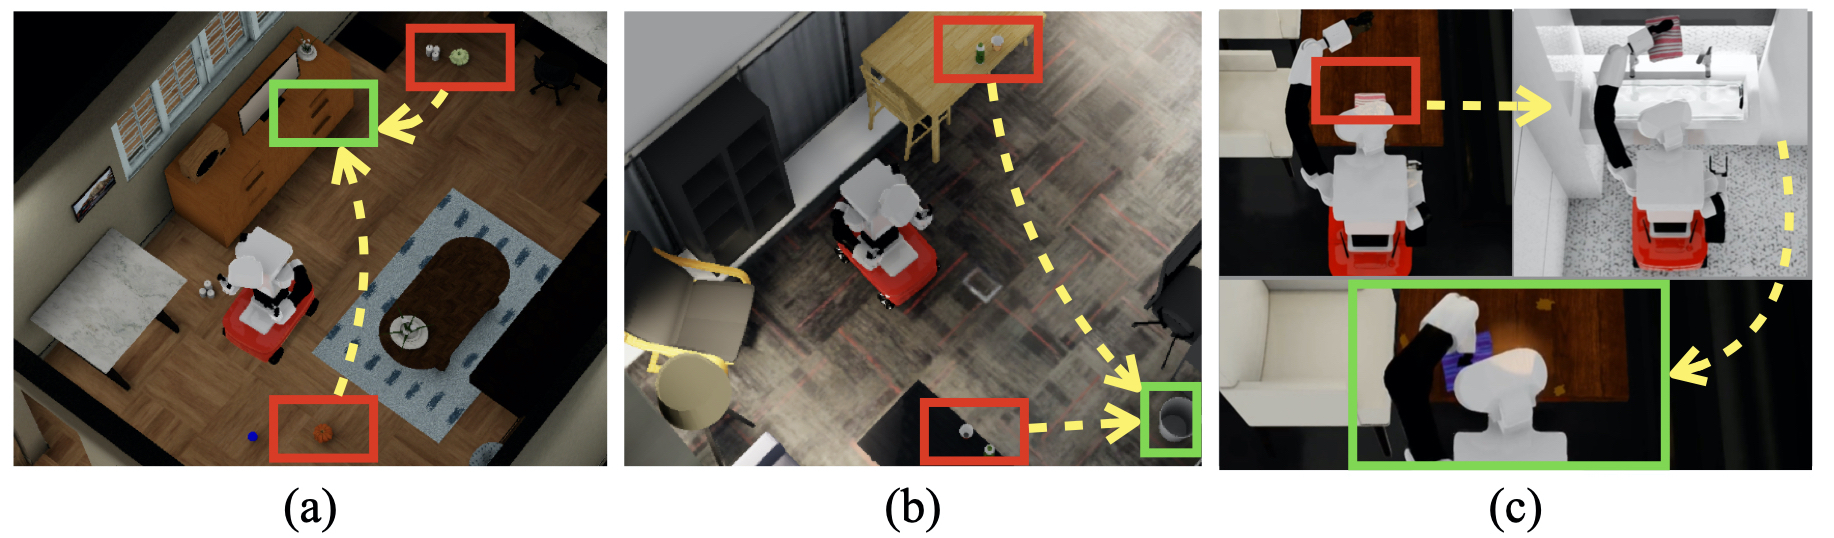
\includegraphics[width=0.95\textwidth]{figures/baseline_appendix/baseline-task.jpeg}
    \caption{\textbf{Activities used in our evaluation.} From left to right: (a). \texttt{StoreDecoration}, (b). \texttt{CollectTrash} and (c). \texttt{CleanTable}. The rectangles indicate relevant locations for the activities, e.g., locations with objects to grasp (\textit{red rectangles}) or to use/place them (\textit{green rectangles}). Even though these activities are some of the most simple in \benchmark, they are still very long-horizon, requiring hundreds of low-level commands or the correct concatenation of multiple action primitives.}
    \label{fig:baseline_task}
\end{figure}

\subsection{Network Architecture}
% \todo{Network details for VMC} 
For \rlprim and \rlprimhist that use PPO as the underlying RL algorithm, the architecture consists of a visual feature extractor that takes the egocentric visual observation as input and a state encoder neural network which takes whether the robot is grasping an object or not as input. The image input is normalized using a per-channel moving average. These two encodings are passed into an MLP module, which is then processed by a value head to predict the value for the given observations and an action head to produce a discrete action that corresponds to an action primitive executed on an object. The size of input images is $128\times 128\times 3$. The feature extractor is a sequential architecture of Conv-ReLU-MaxPooling-Flatten. MLP converts the feature into a $128$-dimensional vector. The details of \rlprim's network architecture is illustrated in Fig.~\ref{fig:appendix_ppo_vmc_arch}~(b). For \rlvmc that uses SAC as the underlying RL algorithm, we use the same feature extractor as \rlprim. \rlvmc consists of an actor network, a critic network, and a target critic network. All of them are MLPs with ReLU activation functions. Fig.~\ref{fig:appendix_ppo_vmc_arch}~(a) illustrates the details of \rlvmc's network architecture. \rlvmc has the continuous action space and outputs low-level control actions directly.

\subsection{Task settings}
Fig.~\ref{fig:baseline_task} depicts the three activities we consider in our experiments: 
\vspace{-2mm}
\begin{itemize}[leftmargin=2em]
    \item \texttt{StoreDecoration}: a tidying activity where the agent must pick up and store Halloween decorations into a cabinet operating articulated objects. Action space: \texttt{navigate}, \texttt{pick}, \texttt{place}, \texttt{push}. The goal is to store two pumpkins into a drawer (see Fig.~\ref{fig:baseline_task} (a)).
    \item \texttt{CollectTrash}: A collecting activity that requires the agent to gather empty bottles and cups and throw them into a trash bin. Action space: \texttt{navigate}, \texttt{pick}, \texttt{place}. The goal is to throw two bottles and two cups into a trash bin (see Fig.~\ref{fig:baseline_task} (b)).
    \item \texttt{CleanTable}: A cleaning activity that involves challenging cloth manipulation and fluids for table cleaning. Action space: \texttt{navigate}, \texttt{pick}, \texttt{dip}, \texttt{wipe}. The goal is to cleaning a table with a soaked cloth (see Fig.~\ref{fig:baseline_task} (c)). 
\end{itemize}
Each activity takes place in a different B1K scene, \texttt{Rs\_int}, \texttt{mockup\_apt}, and \texttt{restaurant\_hotel}. 
%\texttt{Rs\_int} is an enhanced version where YYY is a digital twin of a real mockup apartment, as we will see in Sec.~\ref{sec:sim2real}.

% \begin{figure*}[t]
% \centering
% \begin{minipage}[c]{\linewidth}
% \centering
%     \renewcommand\tabcolsep{0.5pt}
%     \begin{tabular}{ccc}
%         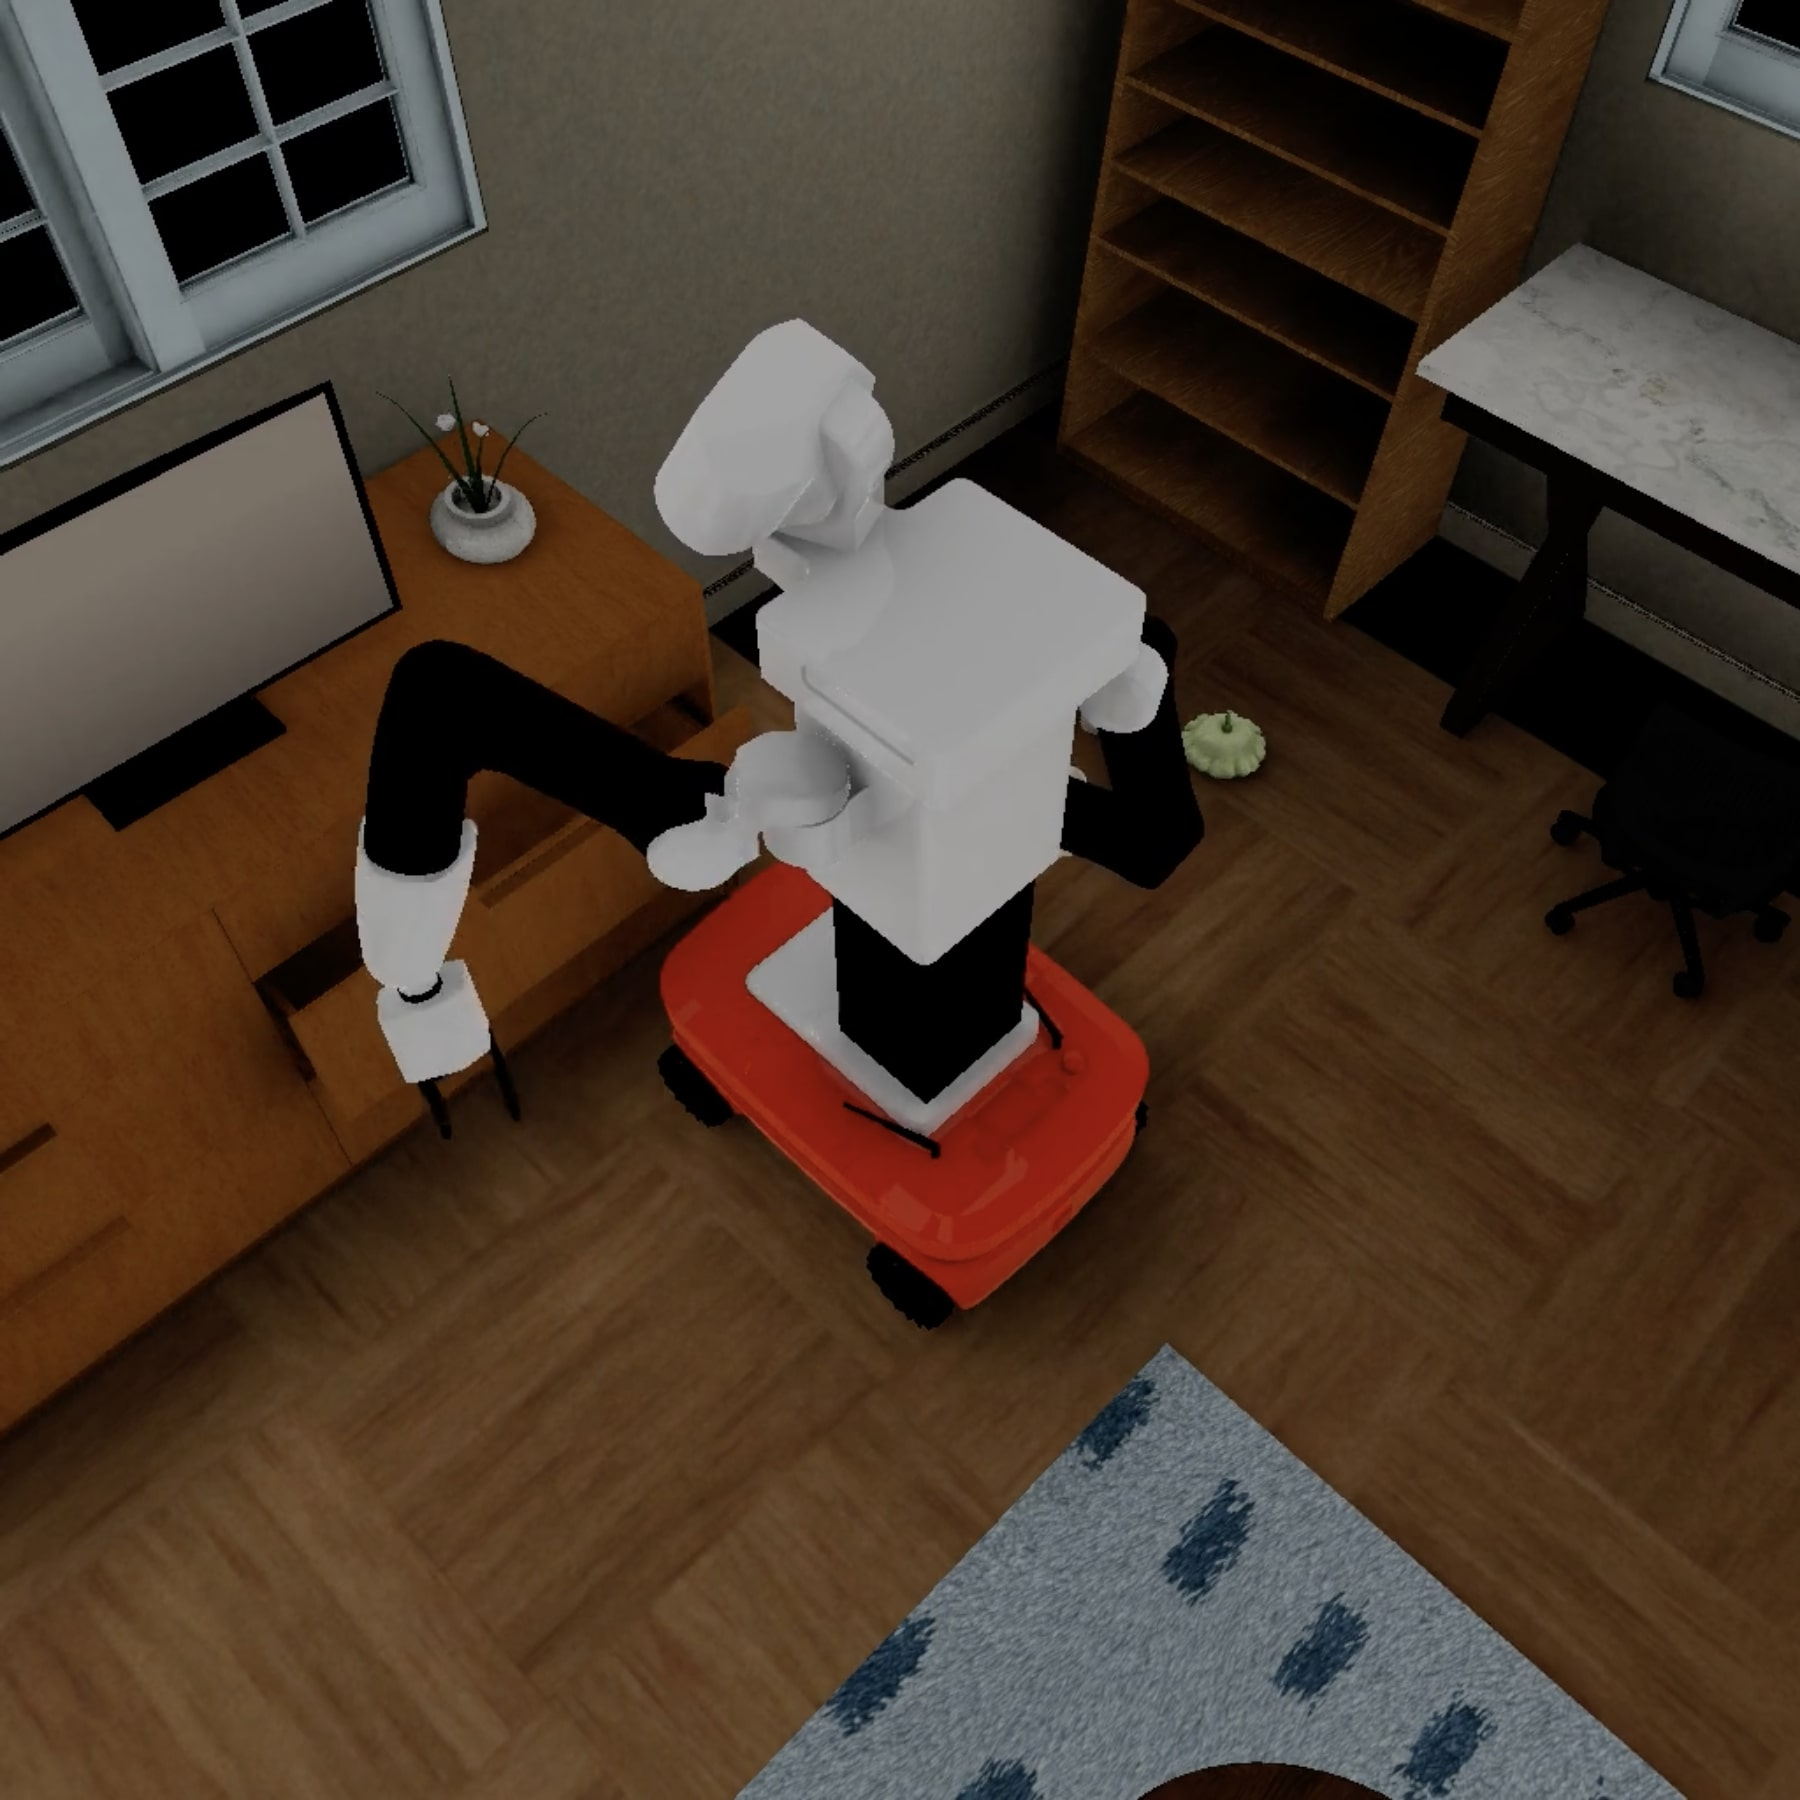
\includegraphics[width=0.3\linewidth]{figures/baseline_appendix/store_decoration_1.png}&
%         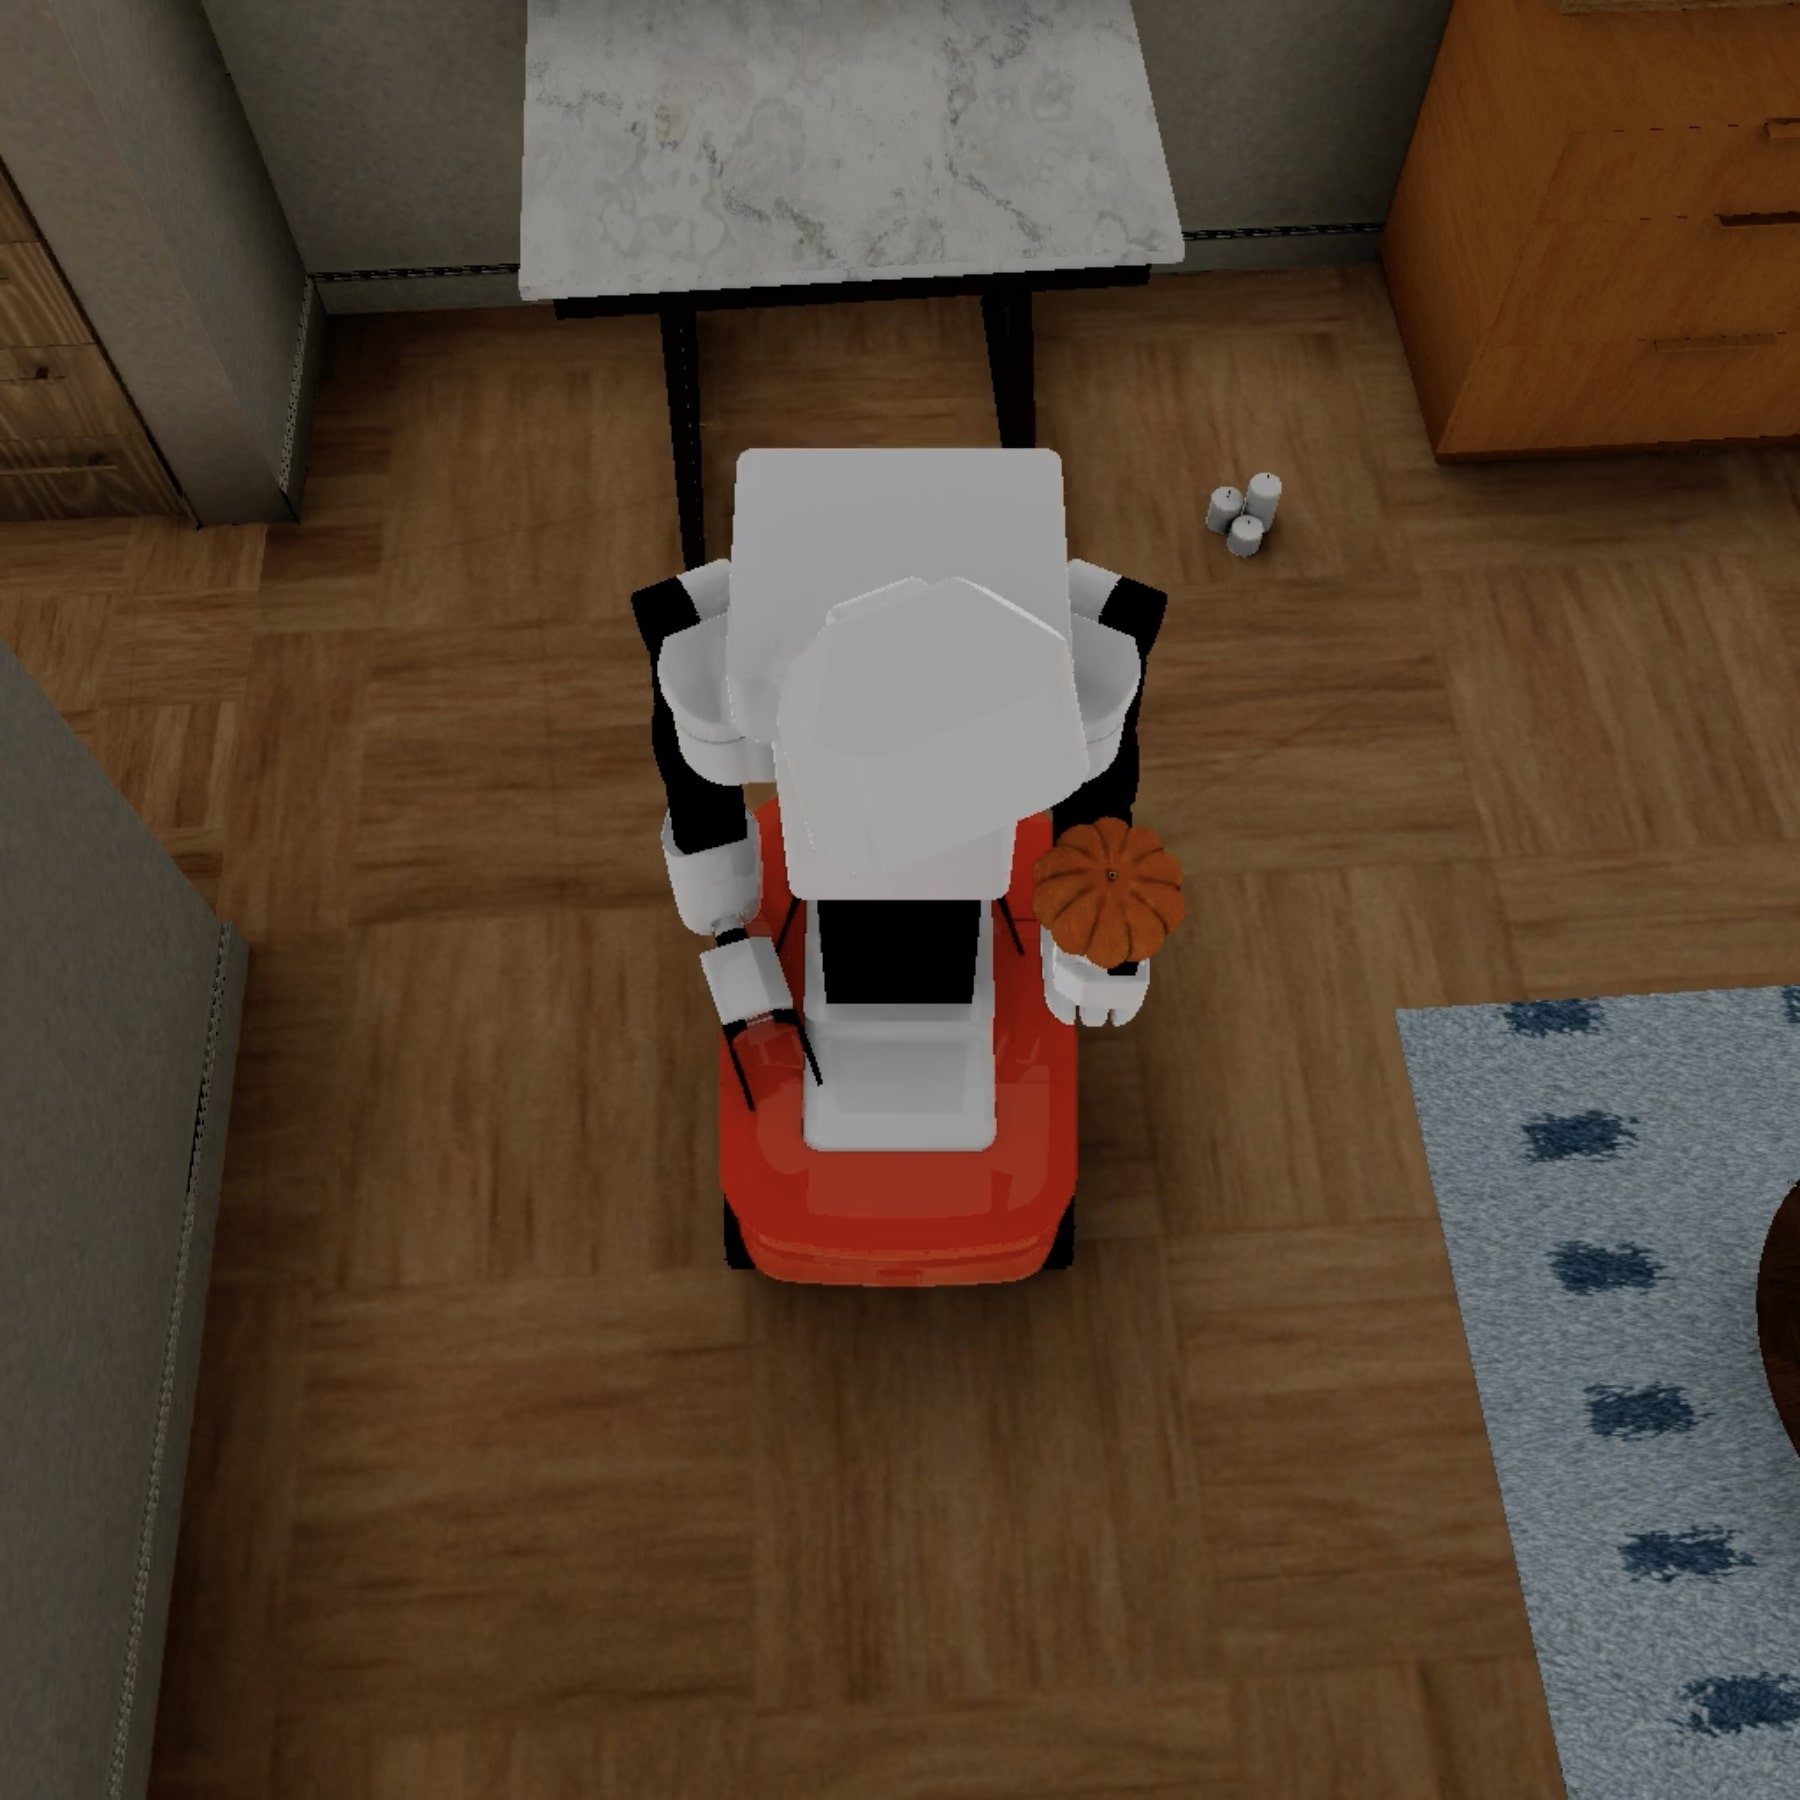
\includegraphics[width=0.3\linewidth]{figures/baseline_appendix/store_decoration_2.png}&
%         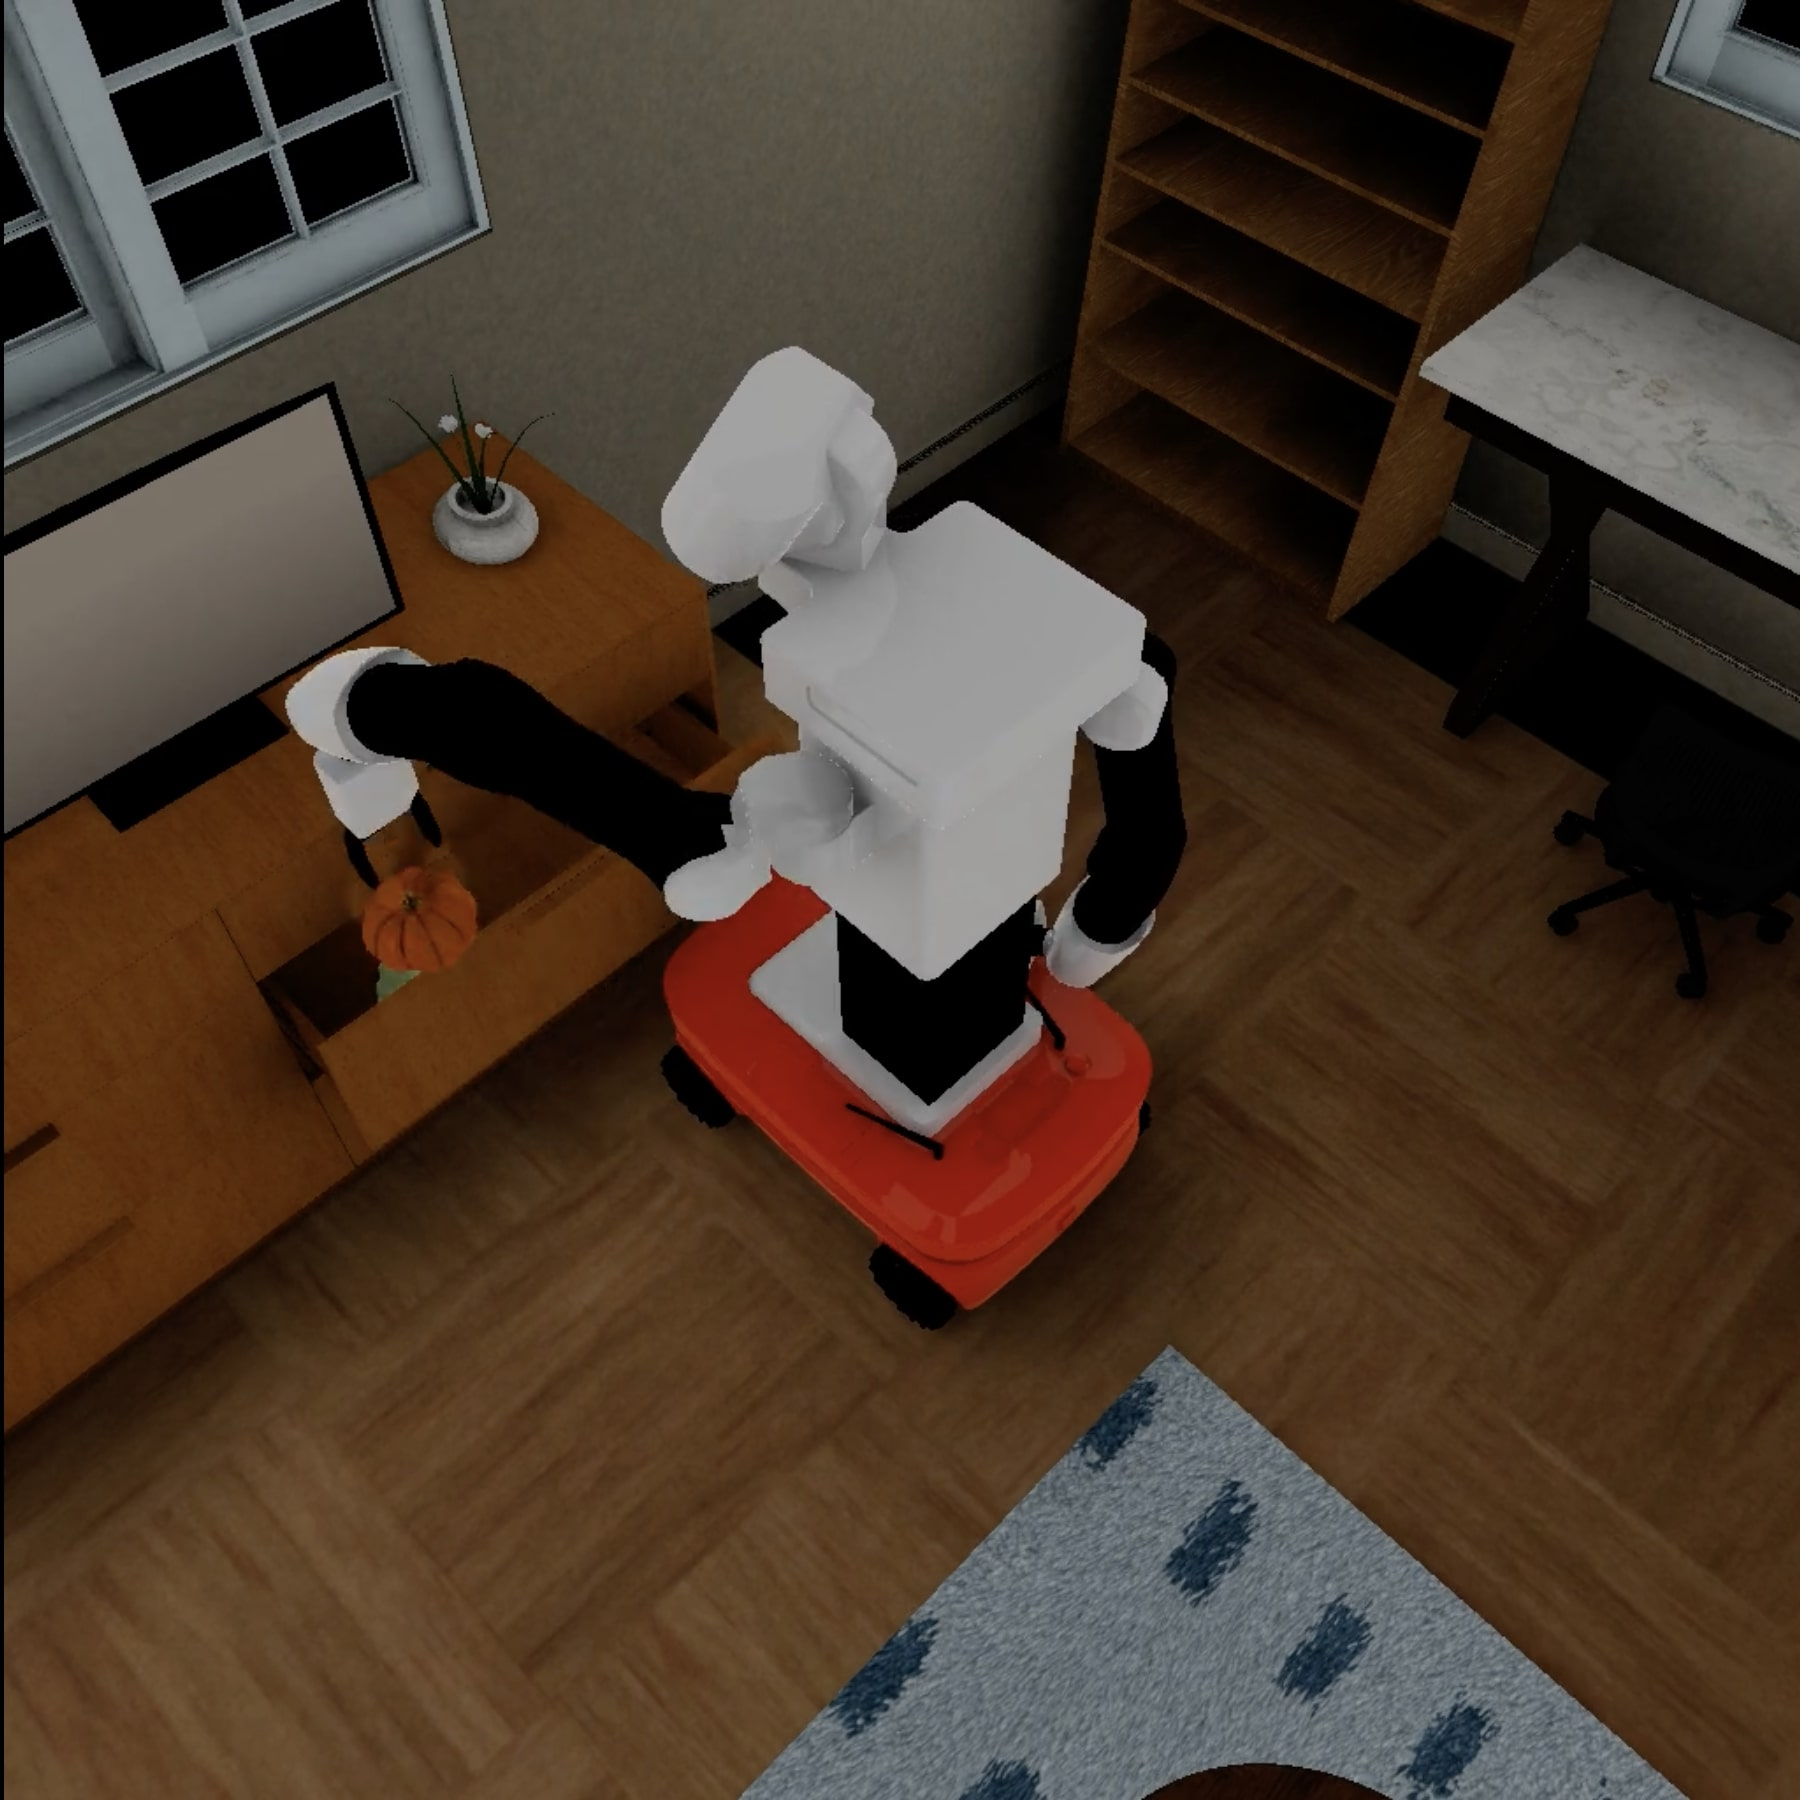
\includegraphics[width=0.3\linewidth]{figures/baseline_appendix/store_decoration_3.png}\\
%         & a) \texttt{StoreDecoration} & \\
%         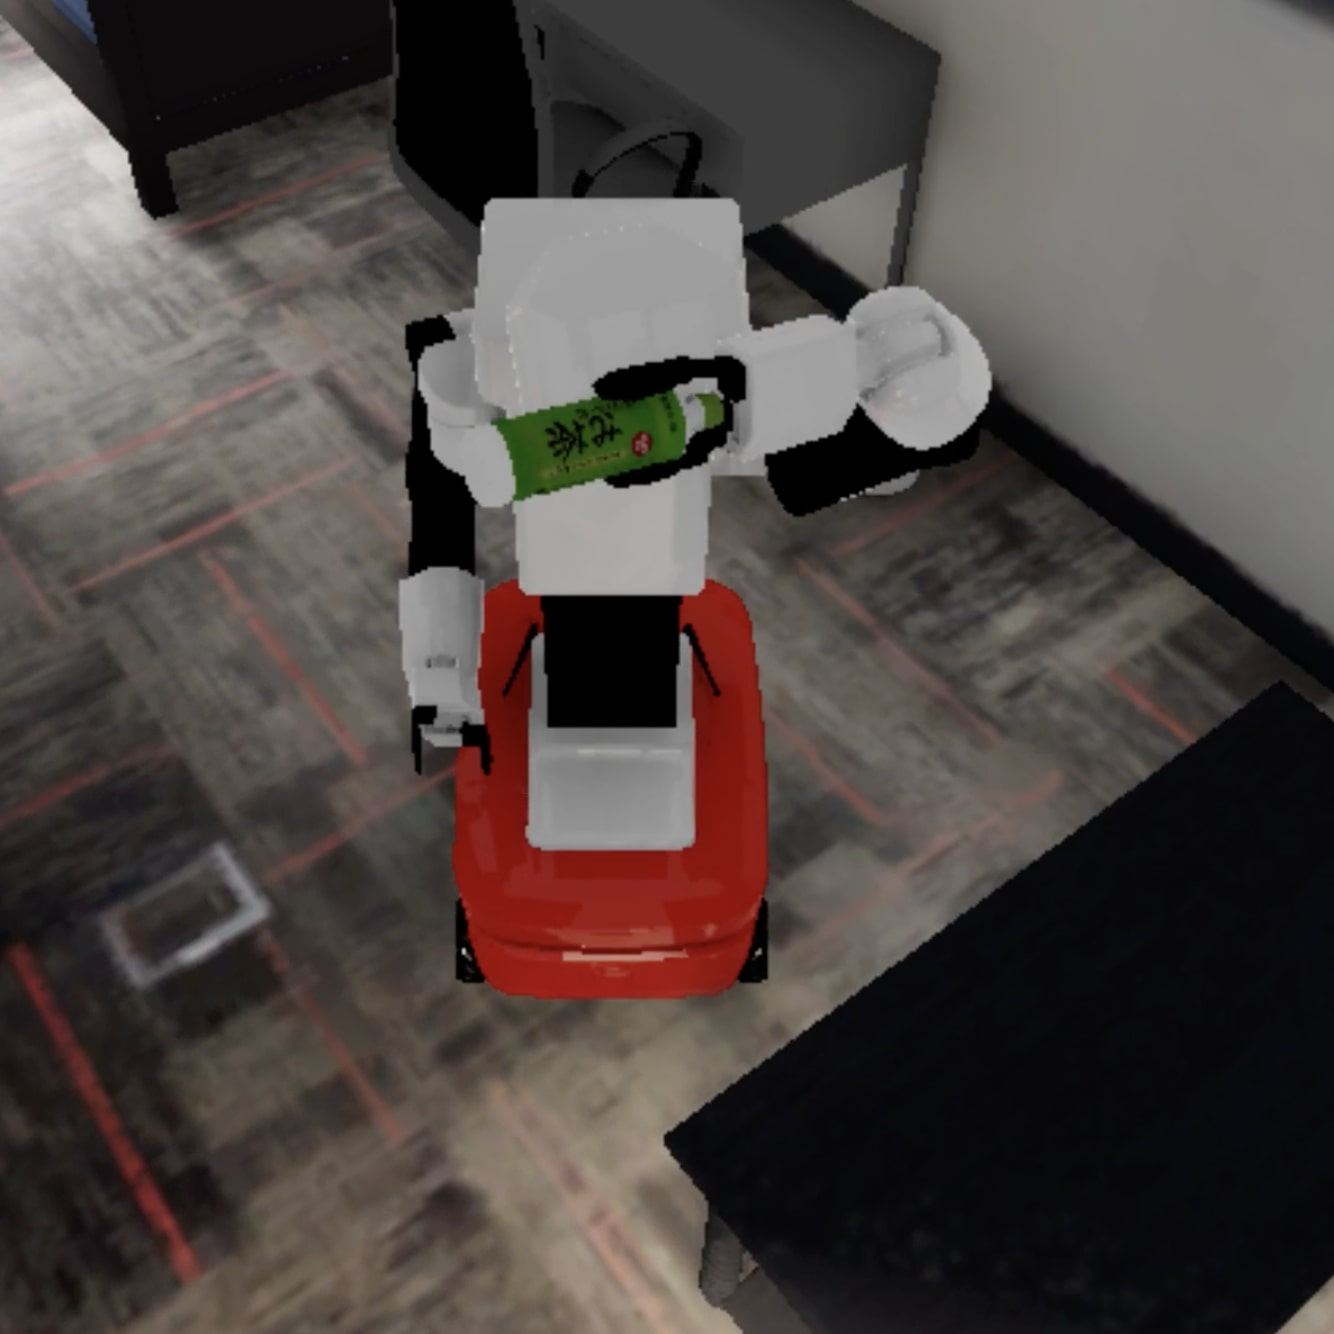
\includegraphics[width=0.3\linewidth]{figures/baseline_appendix/collect_trash_1.png}&
%         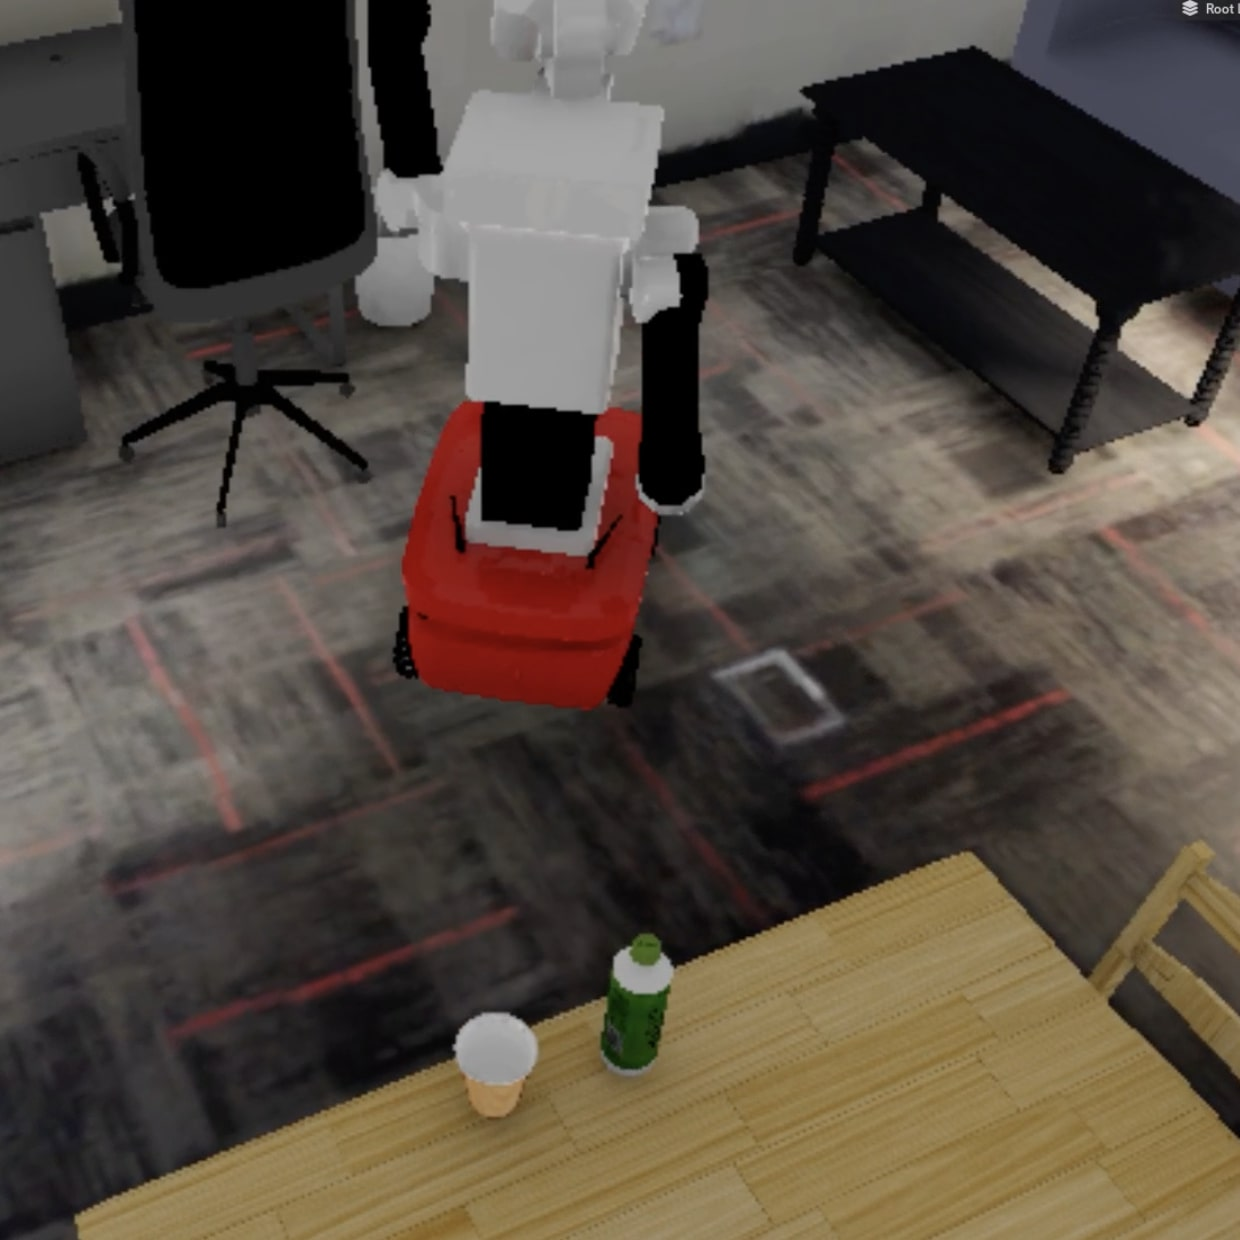
\includegraphics[width=0.3\linewidth]{figures/baseline_appendix/collect_trash_2.png}&
%         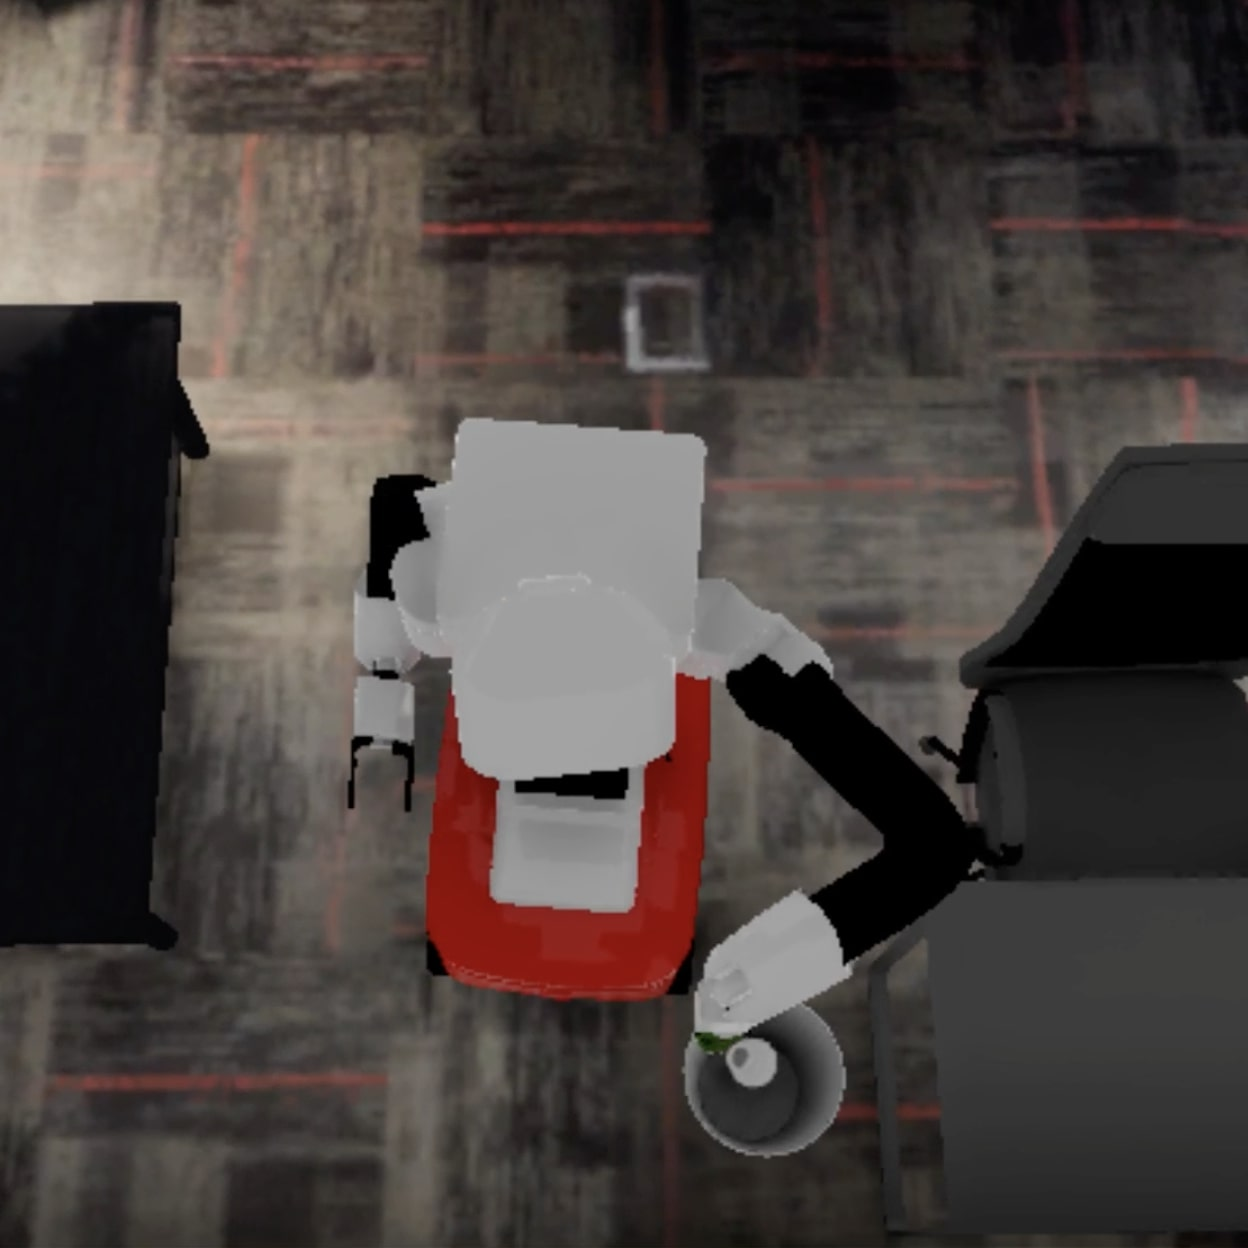
\includegraphics[width=0.3\linewidth]{figures/baseline_appendix/collect_trash_3.png}\\
%         & b) \texttt{CollectTrash} & \\
%         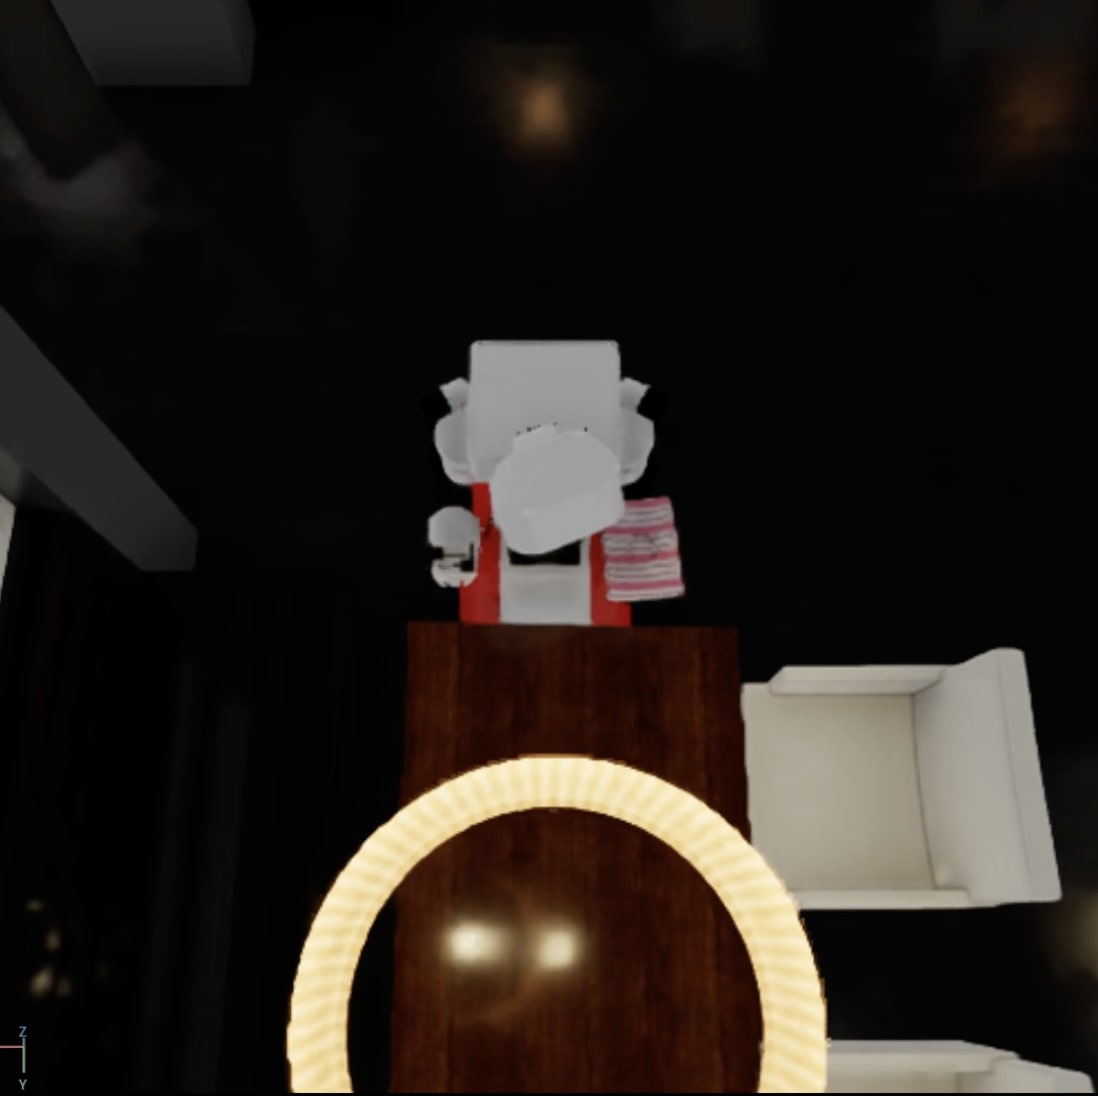
\includegraphics[width=0.3\linewidth]{figures/baseline_appendix/clean_table_1.png}&
%         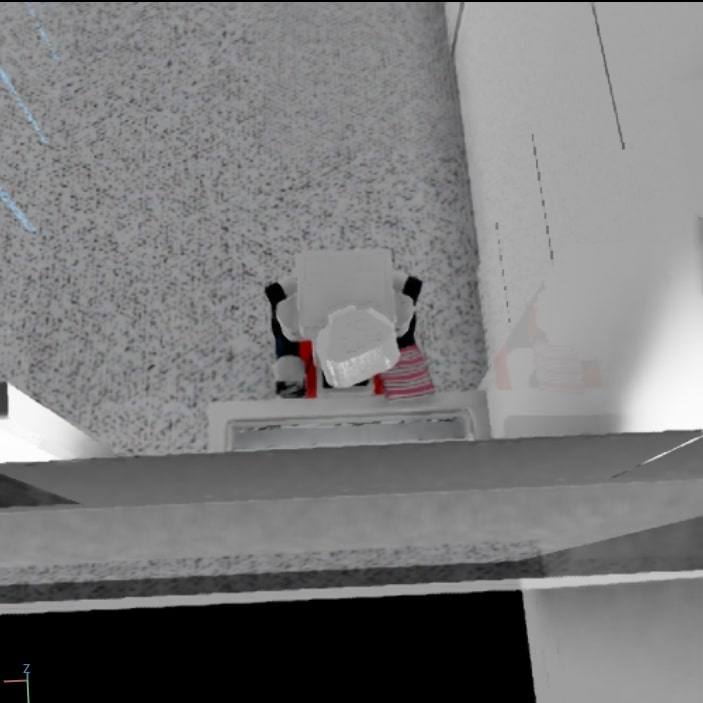
\includegraphics[width=0.3\linewidth]{figures/baseline_appendix/clean_table_2.png}&
%         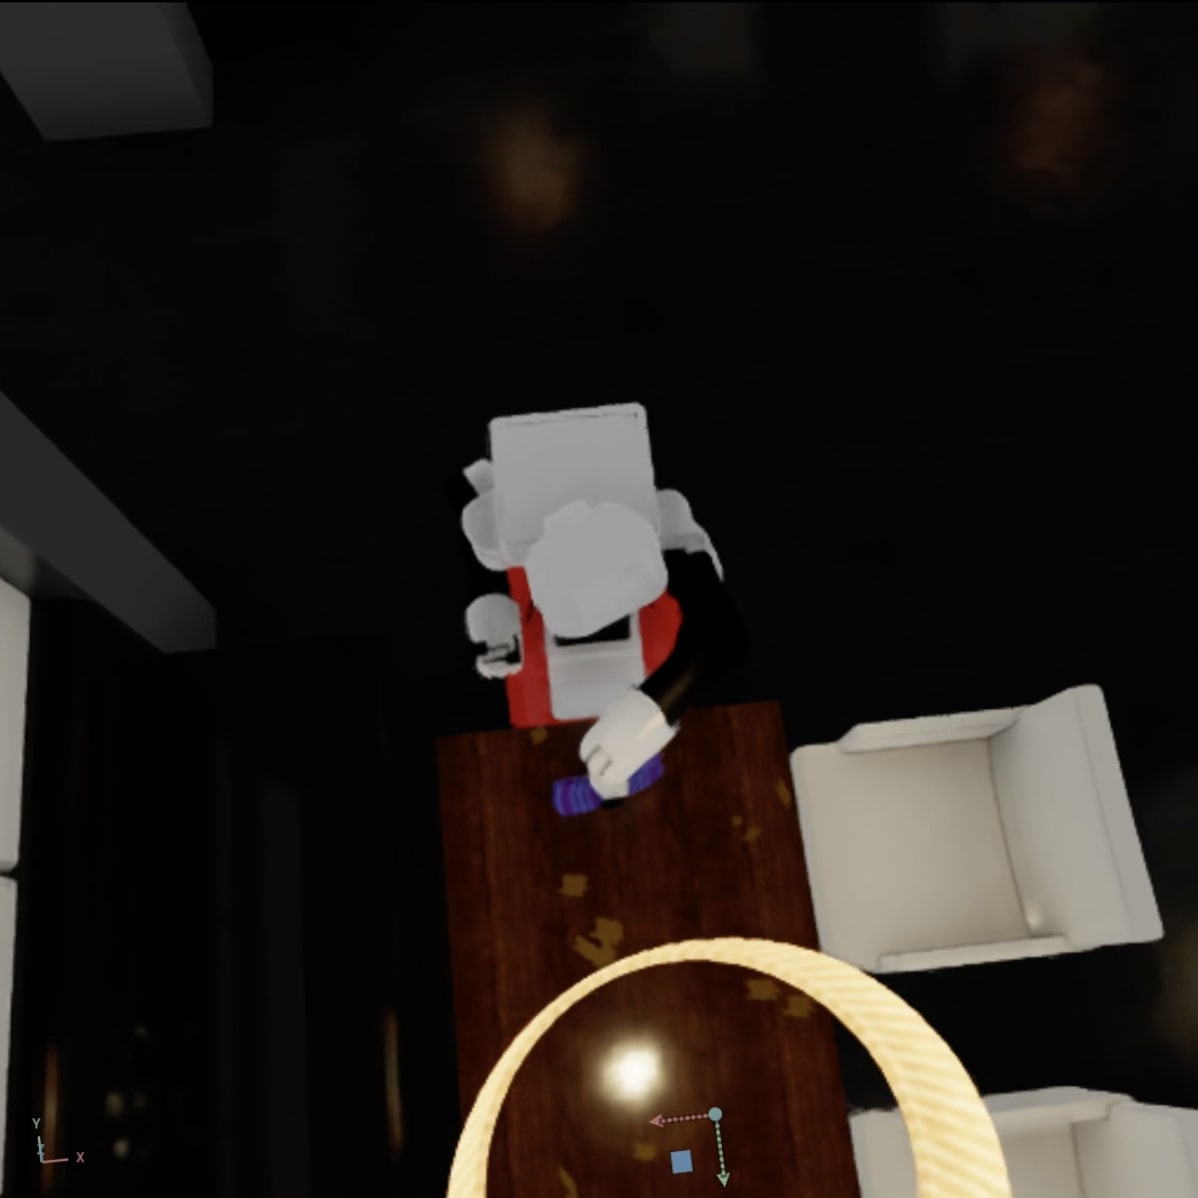
\includegraphics[width=0.3\linewidth]{figures/baseline_appendix/clean_table_3.png}\\
%         & c) \texttt{CleanTable} & \\
%     \end{tabular}
%     \caption{Overview of three tasks: \texttt{StoreDecoration}, \texttt{CollectTrash}, and \texttt{CleanTable}.}
%     \label{fig:appendix_task}
% \end{minipage}
% \end{figure*}


\subsection{Training details}

\paragraph{Learning objectives.} %\todo{Learning objectives for VMC} 
For \rlprim and \rlprimhist, we use an on-policy reinforcement learning algorithm Proximal Policy Optimization (PPO). $\theta$ is the policy parameter, $\hat{E}_t$ denotes the empirical expectation over timesteps. $r_{t}$ is the ratio of the probability under the new and old policies, respectively. $\hat{A}_t$ is the estimated advantage at time $t$. $\epsilon$ is the clipping hyperparameter. The objective function of PPO is shown in Equation~\ref{equ:ppo}:
\begin{equation}
    C^{CLIP}(\theta) = \hat{E}_t[\min r_t(\theta)\hat{A}_t, clip(r_t(\theta), 1-\epsilon, 1+\epsilon)\hat{A}_t].
    \label{equ:ppo}
\end{equation}
For \rlvmc, we use Soft Actor Critic (SAC) algorithm. The objective function is shown in Equation~\ref{equ:sac}:
\begin{equation}
    \pi^* = \arg\max_\pi E_{\tau\sim\pi}\left[\sum_{t=0}^\infty \gamma^t \left(R(s_t, a_t, s_{t+1})+\alpha H (\pi(\cdot|s_t)\right)\right],
    \label{equ:sac}
\end{equation}
where $\alpha$ is the coefficient that determines the weight of two terms and $H$ denotes the entropy.

\paragraph{Reward function.} %\todo{Reward for VMC, it should be the same as primitives baseline?} 
We use the success signal provided by the BDDL activity definition as the reward function for training the policy in all methods. For instance, in the \texttt{StoreDecorations} task, the BDDL task goal definition is \texttt{Forall(decoration)\{Inside(decoration, cabinet)\}}. The agent receive a positive signal if and only if one of the \texttt{decoration} is physically placed inside the \texttt{drawer} of the \texttt{cabinet}. This is a challenging sparse reward setting since the agent needs to plan multiple steps to reach the final goal without any intermediate subgoal rewards (e.g. \texttt{push} open the \texttt{drawer} must take place before \texttt{pick} and \texttt{place} the \texttt{decoration}, but no reward signal will be given to the \texttt{push} open action).% VMC uses the same reward function as other baselines.

\paragraph{Hyperparameters.} %\todo{Hyperparameters for VMC} 
The hyperparameters for SAC and PPO in the baselines are summarized in Table~\ref{tab:vmc_hyper_param} and Table~\ref{tab:ppo_hyper_param}. Both SAC and PPO are trained for 30,000 time steps. We train with seeds $0, 1, 2$ and evaluate with seed $0$.

\paragraph{Computation.}
\revision{For each run of our experiments, we use either a single Nvidia GeForce RTX 2080 Ti or a single Nvidia RTX A-6000 GPU, together with Intel Xeon CPU, and 40GB of RAM. During training, the GPU memory usage is around 9GB. Depending on which task, the total training iterations range between 10k to 25k, and the total wall-clock training time range between 3.75 to 7.5 hours.}

\begin{table}[t]
\centering
\begin{minipage}[t]{.41\linewidth}%
    \begin{tabular}{c|c}
    \toprule
        Learning Rate & $0.0003$ \\
        Buffer Size & $300$ \\
        Batch Size &  $64$ \\
        Discount ($\gamma$) & $0.99$ \\
        Soft Update Coefficient & $0.005$ \\
    \bottomrule
    \end{tabular}
    \caption{Hyperparameters of SAC for the \rlvmc baseline}
    \label{tab:vmc_hyper_param}
\end{minipage}
\hfill
\begin{minipage}[t]{.41\linewidth}%
    \begin{tabular}{c|c}
    \toprule
        Learning Rate & $0.0003$ \\
        Buffer Size & $300$ \\
        Batch Size &  $64$ \\
        Discount ($\gamma$) & $0.99$ \\
        GAE Parameter $\gamma_{gae}$ & $0.99$ \\
        Clipping Parameter $\epsilon$ & $0.2$ \\
        Entropy Coeff $c_1$ & $0.0$ \\
        VF Coeff $c_2$ & $0.5$ \\
    \bottomrule
    \end{tabular}
    \caption{Hyperparameters of PPO for the \rlprim and \rlprimhist baselines}
    \label{tab:ppo_hyper_param}
\end{minipage}
\end{table}

\subsection{Action Primitives} 
\benchmark activities are long-horizon which require hundreds if not thousands of environment steps (low-level robot control signals) to be completed.  A way to overcome this challenge (e.g., reinforcement learning) is to modify the original action space with a set of \textit{action primitives}, i.e., time-extended actions that correspond to multiple low-level commands and that achieve some expected outcome, such as grasping an object or navigating to a location. For our baselines, we defined six of these primitives, and implemented them using a sampling-based motion planner.

All the primitives are compositional: collision-free paths of the entire robot to navigate to a location, collision-free paths of the robot's arm to reach a \texttt{6D\_pose} with the end-effector, or a predefined arm joint configuration, trajectories where the end-effector follows a \texttt{line} in Cartesian space, possibly colliding/interacting with the environment, and sequences of actions to \texttt{open}/\texttt{close} the robot's gripper while holding the position.
All manipulation primitives start with a trajectory to move the arm from a tucked configuration (folded arm) to an untucked configuration to enable subsequent arm interaction, and end with the inverse motion, from untucked to tucked configuration, to allow subsequent collision-free navigation.
The action primitives take as parameter an object to apply the action on; we assume access to the 3D position of the objects to obtain the necessary parameters to query the motion planner. This procedure is replicated on the real robot, where we combine detections from YOLO~\cite{redmon2018yolov3} with information from the depth map of the RGB-D images to obtain the parameters (see Sec.~\ref{as:s2r}). For the navigation actions, we assume a set of known relevant locations to navigate to (next to the rectangles in Fig.~\ref{fig:baseline_task}) 

The primitives we used in our experiments can be seen in Fig.~\ref{fig:appendix_high_level_planner} and include:
\vspace{-2mm}
\begin{itemize}[leftmargin=2em]
\item[a)] \texttt{navigate}: Collision-free trajectory of the entire robot to a location.
\item[b)] \texttt{pick}: Composition of 1) a trajectory to a pre-grasp \texttt{6D\_pose} above the object to pick, 2) a \texttt{line} trajectory in Cartesian space down towards the object, interrupted when there is contact, 3) a \texttt{closing} action, 4) a first retracting trajectory following a \texttt{line} upwards, and 5) a second retracting trajectory to reach the untucked joint configuration. The primitive only executes if the robot is not currently picking another object.
\item[c)] \texttt{place}: Composition of 1) a trajectory to a pre-place \texttt{6D\_pose} above the object to place the grasped object on, 2) an \texttt{opening} action, 3) a second retracting trajectory to reach the untucked joint configuration. The primitive only executes if the robot is currently holding an object.
\item[d)] \texttt{push}: Composition of 1) a trajectory to a pre-push \texttt{6D\_pose} above the object to push-open, 2) a \texttt{line} trajectory in Cartesian space down towards the object, interrupted if there is contact, 3) a \texttt{line} trajectory in Cartesian space to push-open the object, e.g., towards the robot, 4) a first retracting trajectory following a \texttt{line} upwards, and 5) a second retracting trajectory to reach the untucked joint configuration. 
\item[e)] \texttt{dip}: Composition of 1) a trajectory to a pre-dip \texttt{6D\_pose} above the object to dip into, 2) a \texttt{line} trajectory in Cartesian space down towards the object to dip, 3) a \texttt{line} trajectory in Cartesian space upwards, and 4) a retracting trajectory to reach the initial joint configuration. The primitive only executes if the robot is currently holding an object.
\item[f)] \texttt{wipe}: Composition of 1) a trajectory to a pre-wipe \texttt{6D\_pose} above the object to wipe, 2) a \texttt{line} trajectory in Cartesian space down towards the object to be wiped, interrupted when there is contact, 3) a \texttt{line} trajectory in Cartesian space horizontally to wipe left-right, 4) a \texttt{line} trajectory in Cartesian space horizontally to wipe towards the robot, 4) a first retracting trajectory following a \texttt{line} upwards, and 5) a second retracting trajectory to reach the untucked joint configuration. The primitive only executes if the robot is currently holding an object.
\end{itemize}

% \begin{figure}[h!]
% \centering
%     \renewcommand\tabcolsep{0.5pt}
%     \begin{tabular}{ccc}        
%         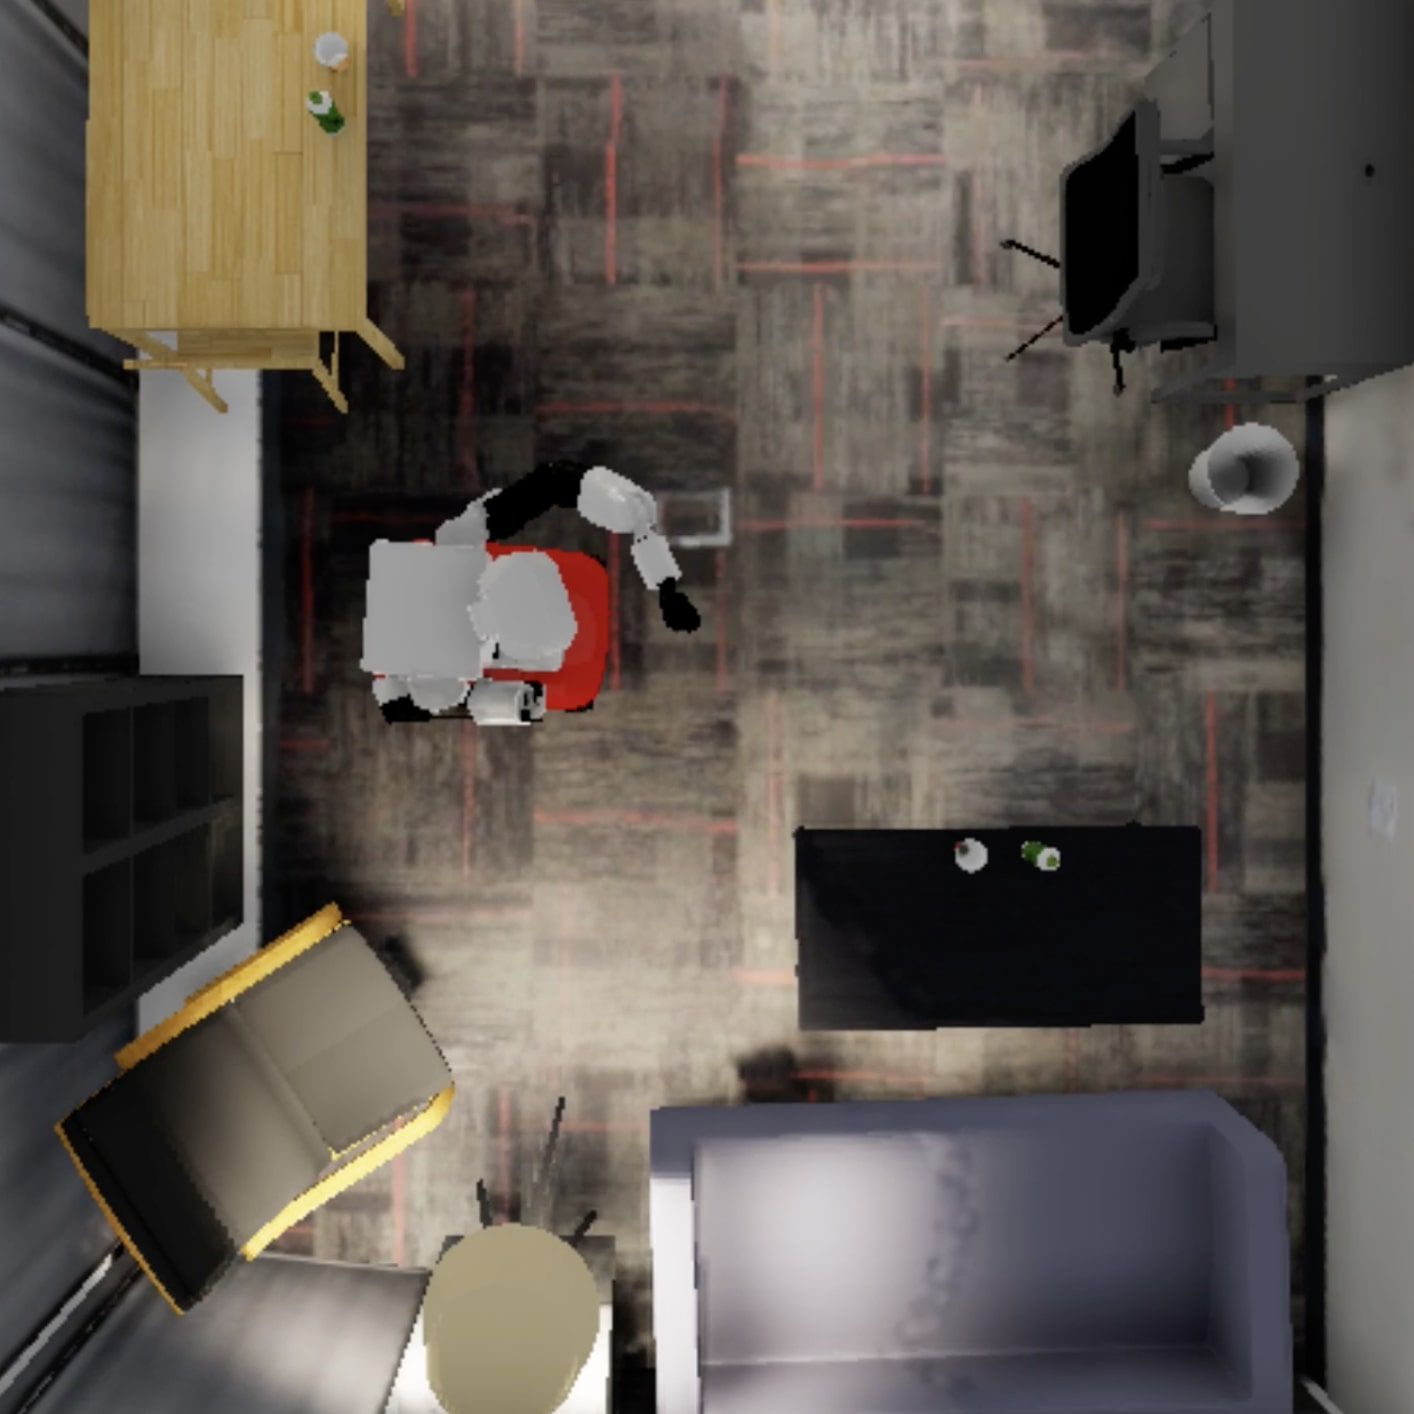
\includegraphics[trim=0 200 0 200,clip,width=0.3\linewidth]{figures/baseline_appendix/navigate_to_1}&
%         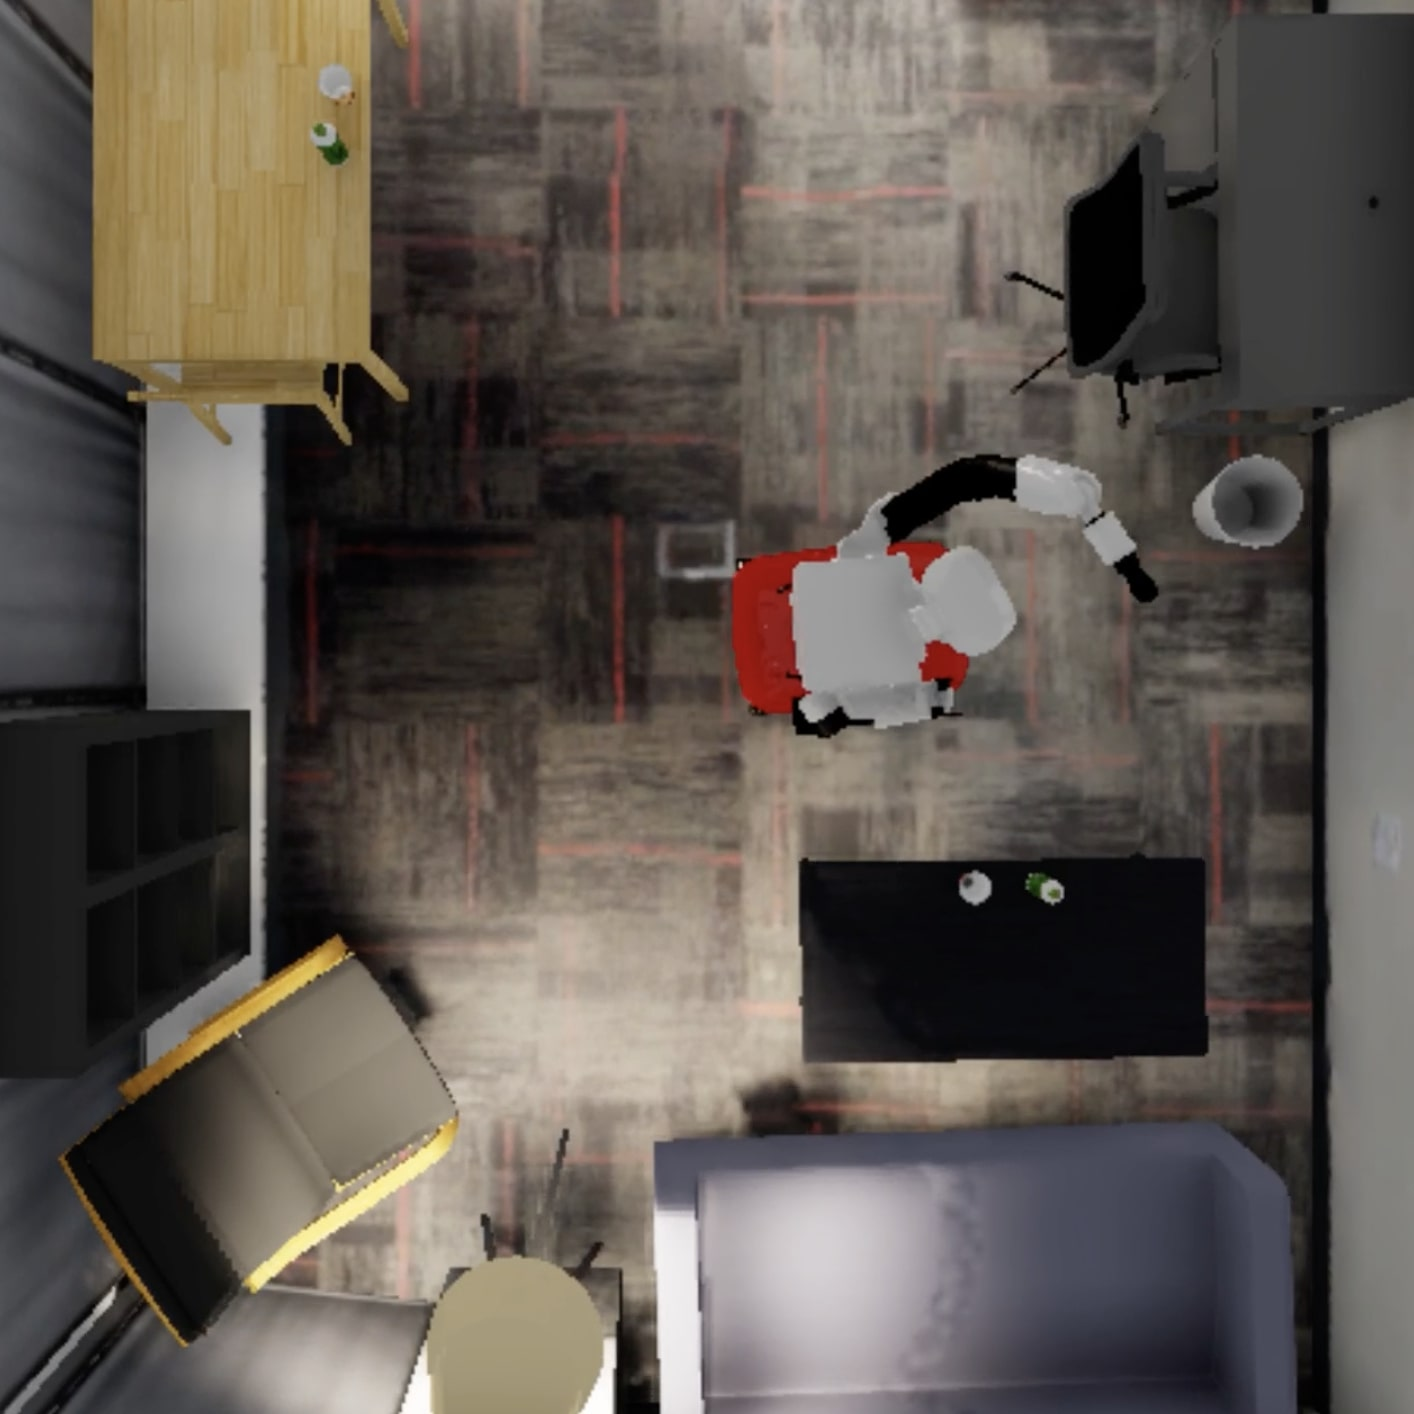
\includegraphics[trim=0 200 0 200,clip,width=0.3\linewidth]{figures/baseline_appendix/navigate_to_2}&
%         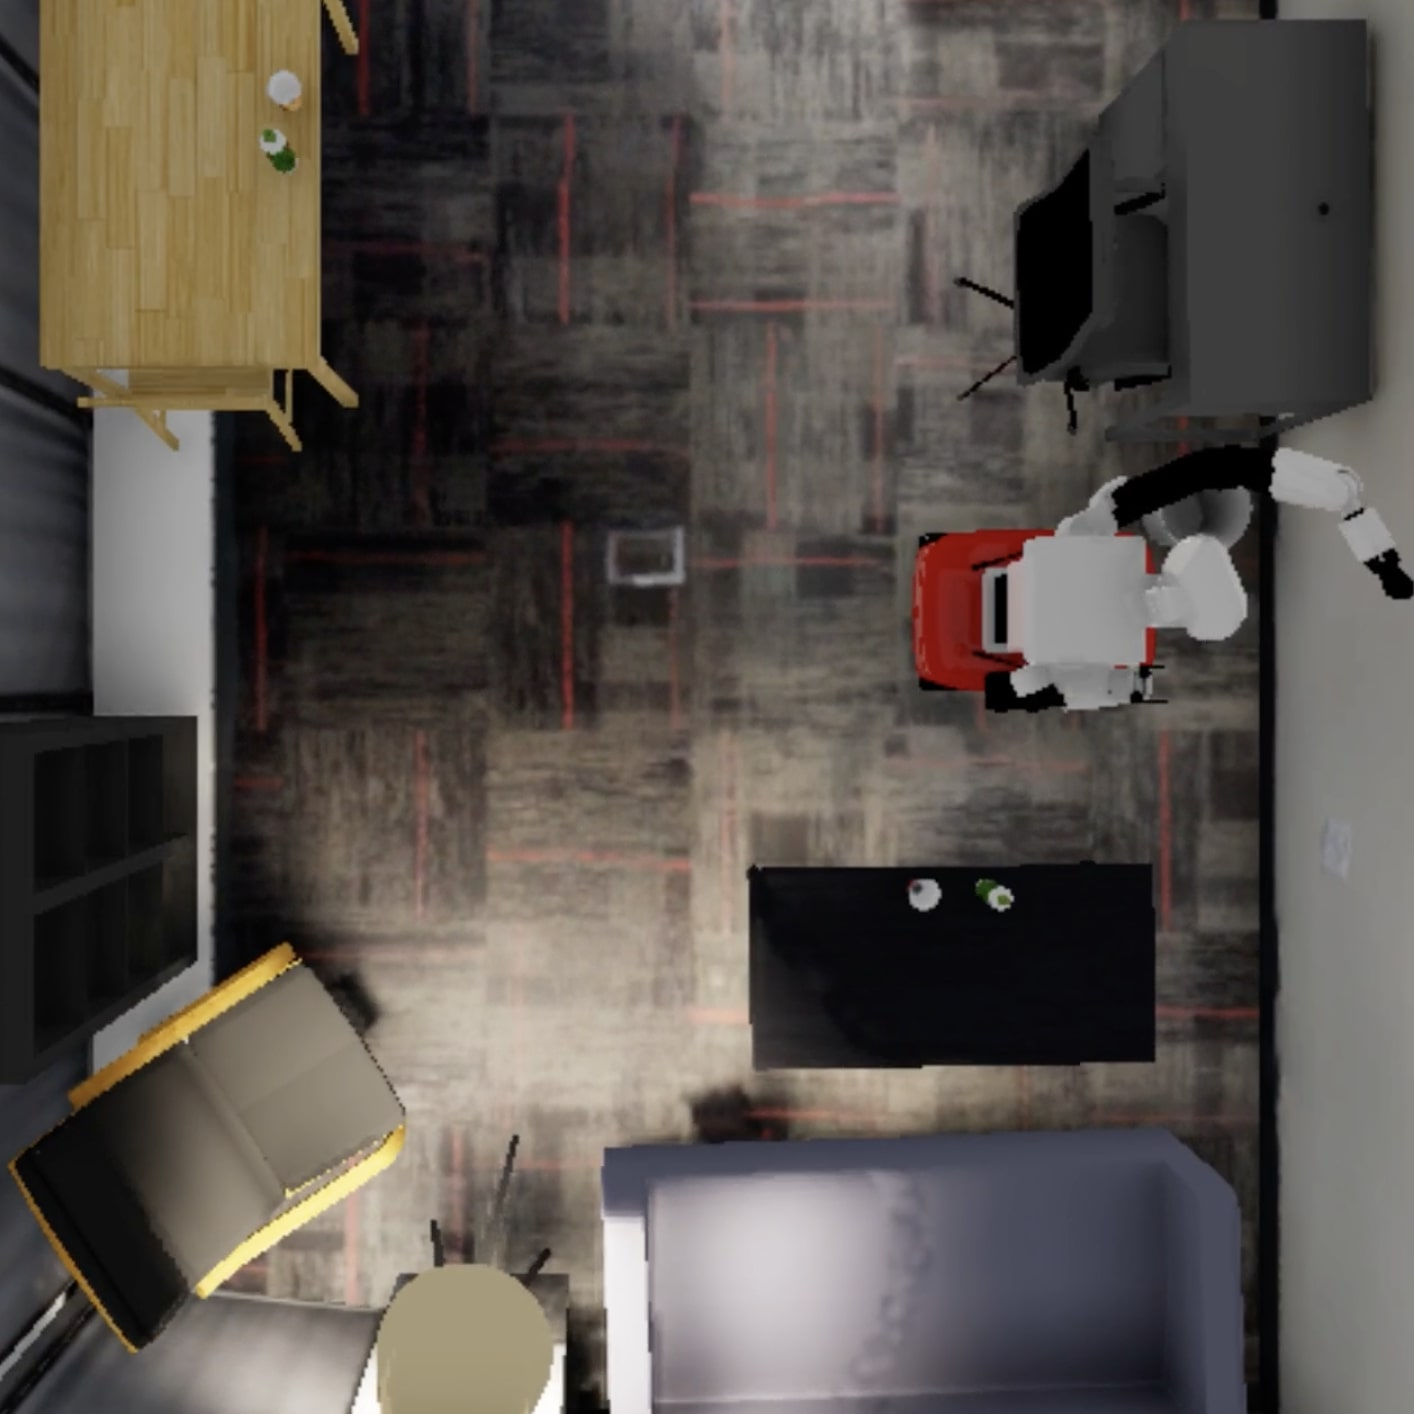
\includegraphics[trim=0 200 0 200,clip,width=0.3\linewidth]{figures/baseline_appendix/navigate_to_3}\\
%         & a) \texttt{navigate} & \\
%         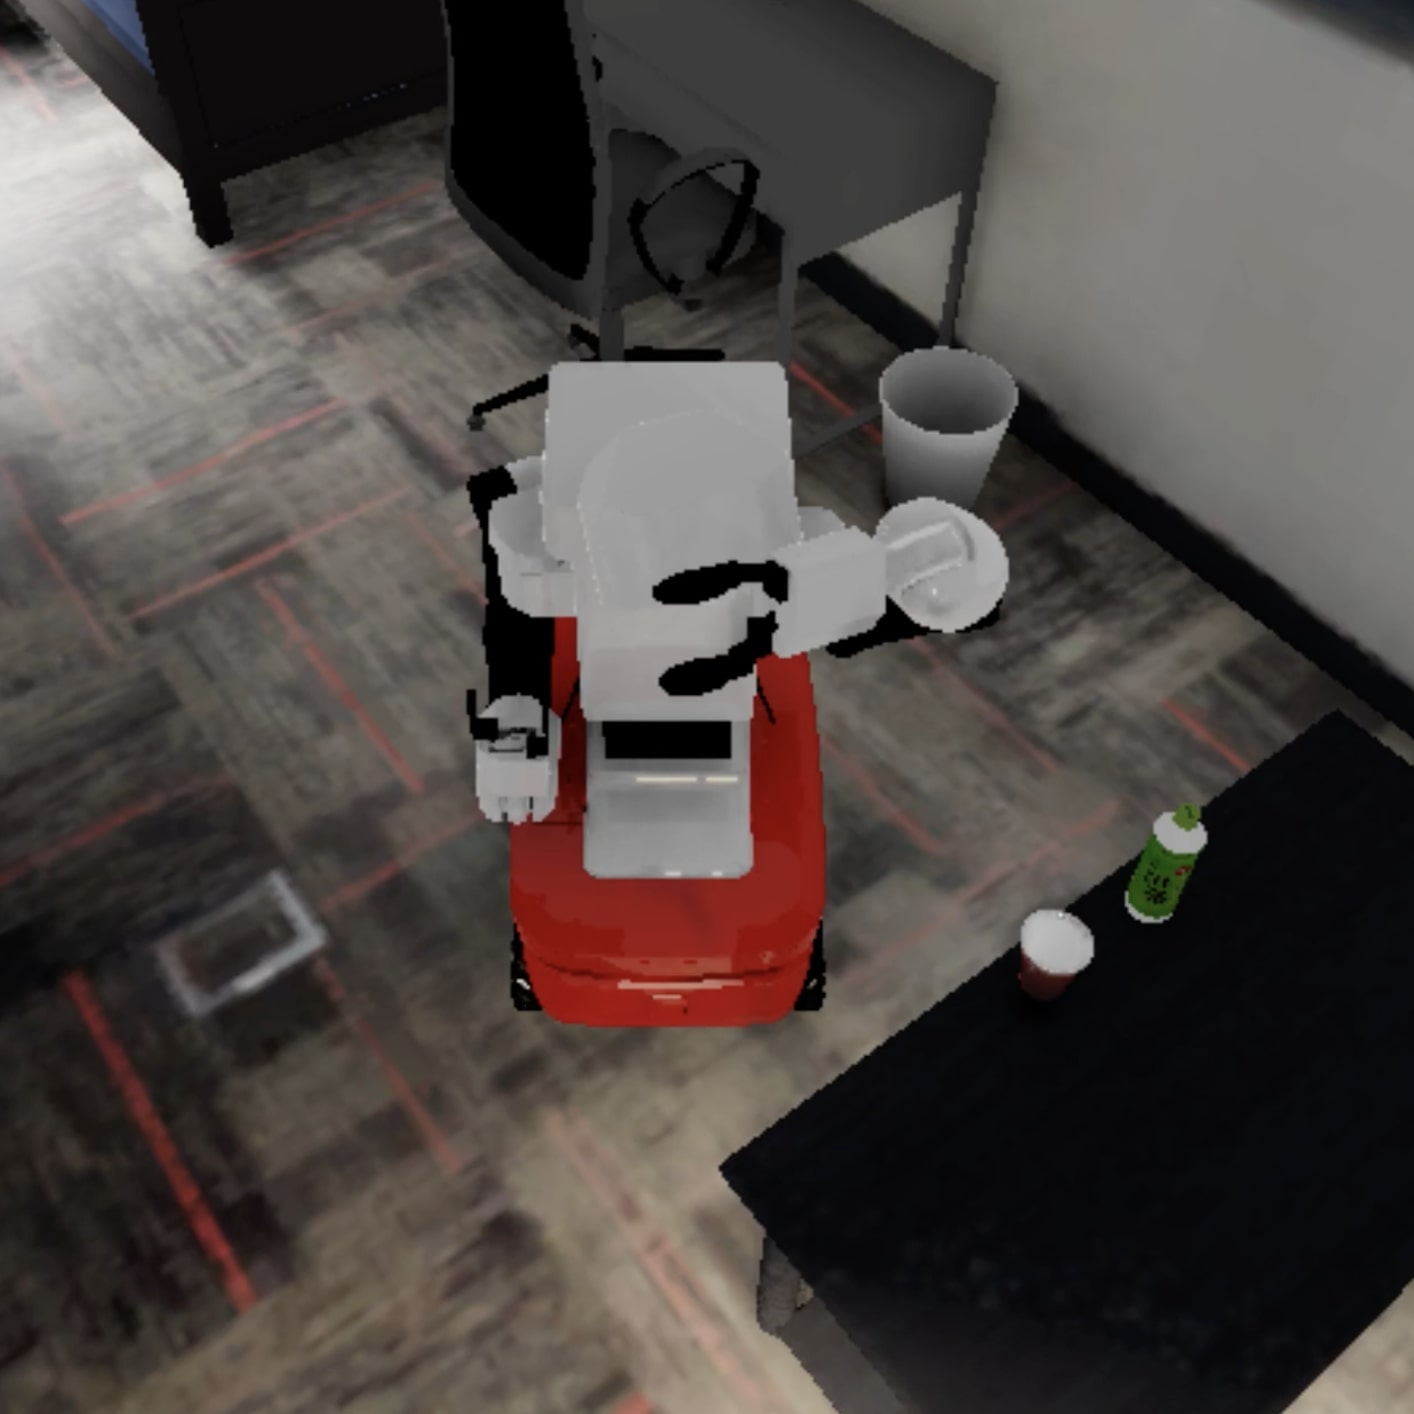
\includegraphics[trim=0 200 0 200,clip,width=0.3\linewidth]{figures/baseline_appendix/pick_1}&
%         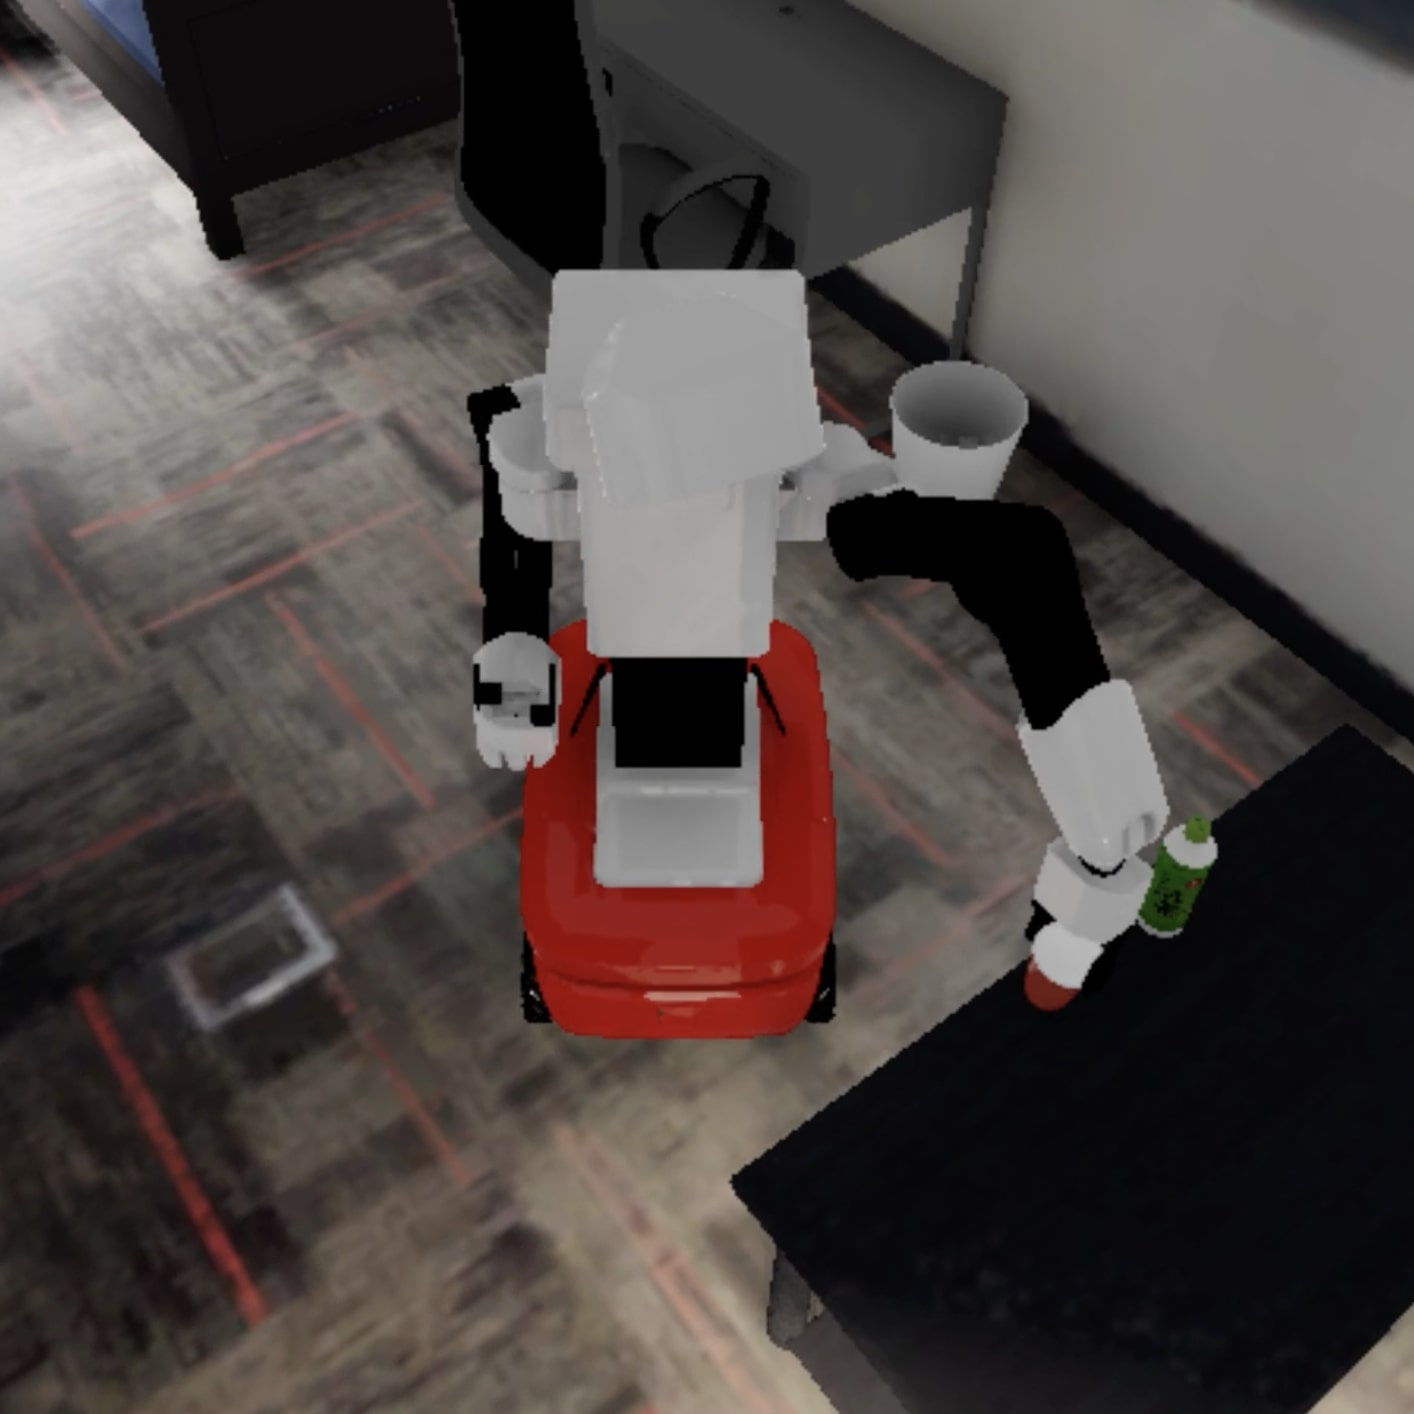
\includegraphics[trim=0 200 0 200,clip,width=0.3\linewidth]{figures/baseline_appendix/pick_2}&
%         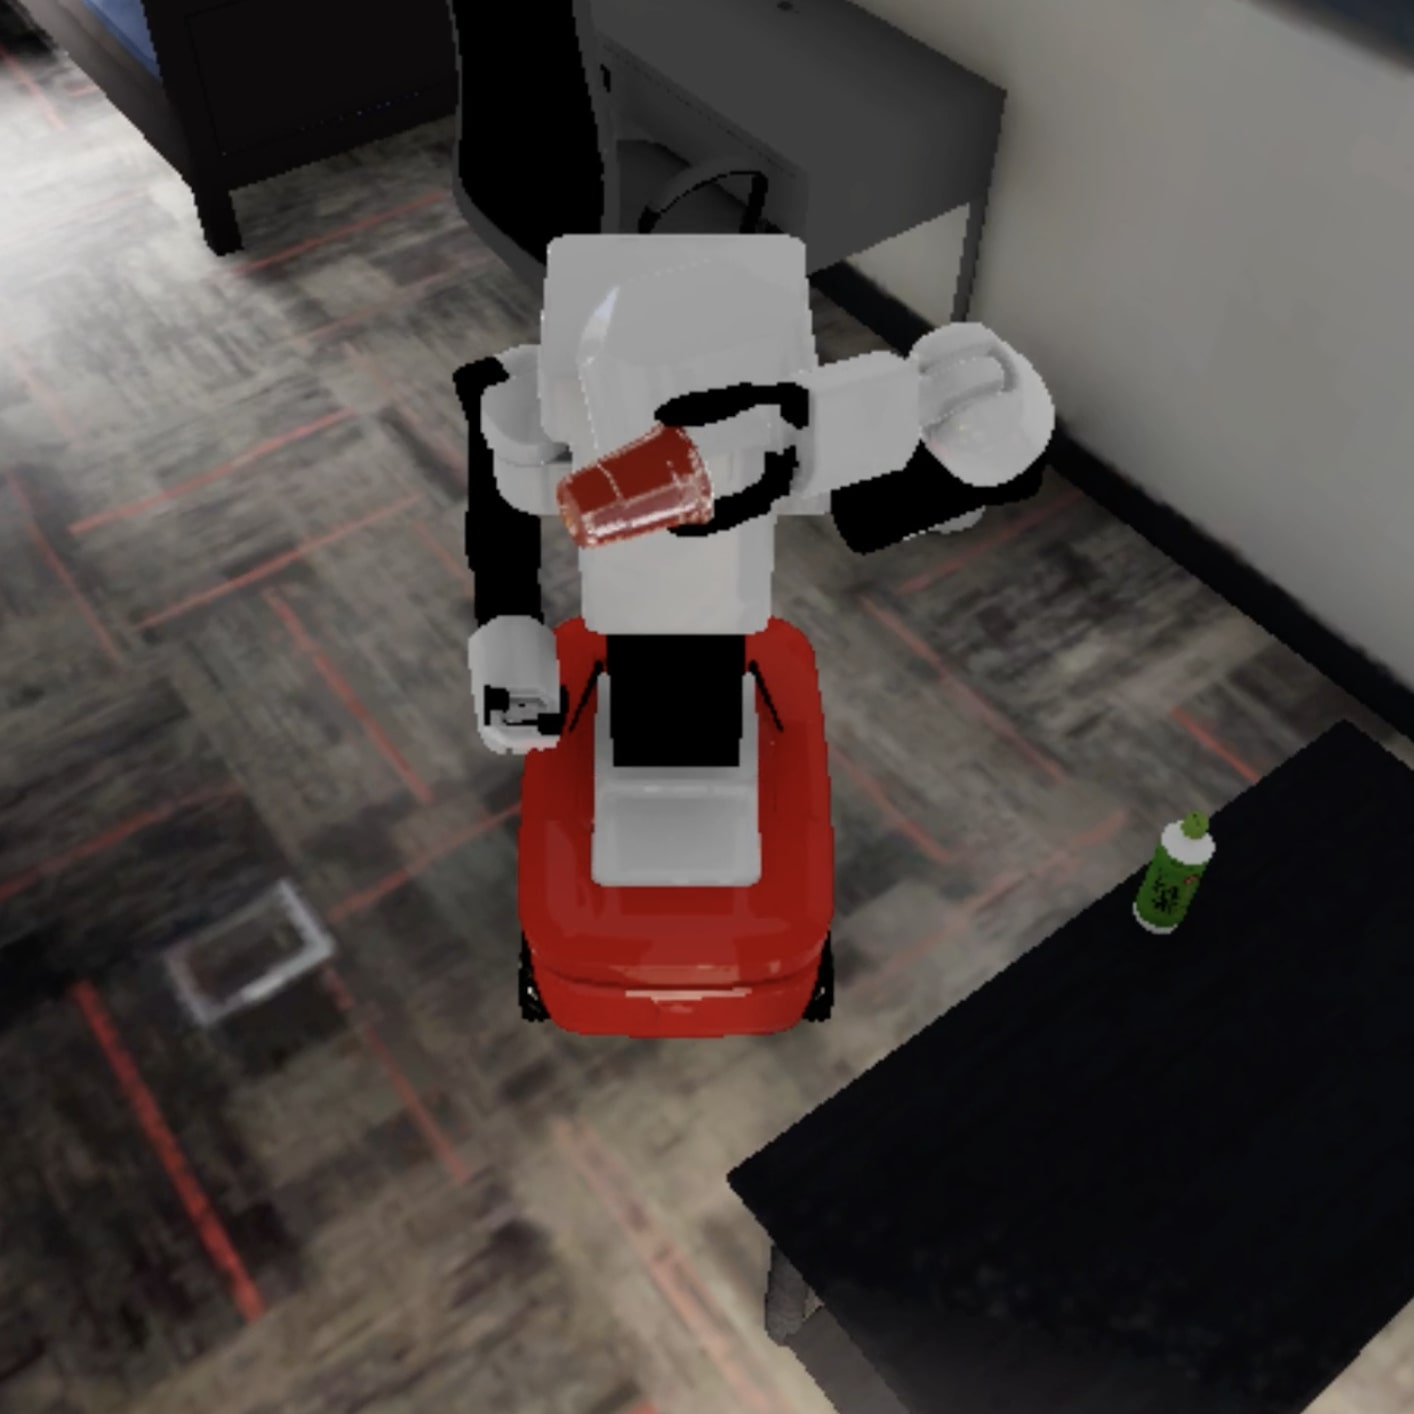
\includegraphics[trim=0 200 0 200,clip,width=0.3\linewidth]{figures/baseline_appendix/pick_3}\\
%         & b) \texttt{pick} & \\
%         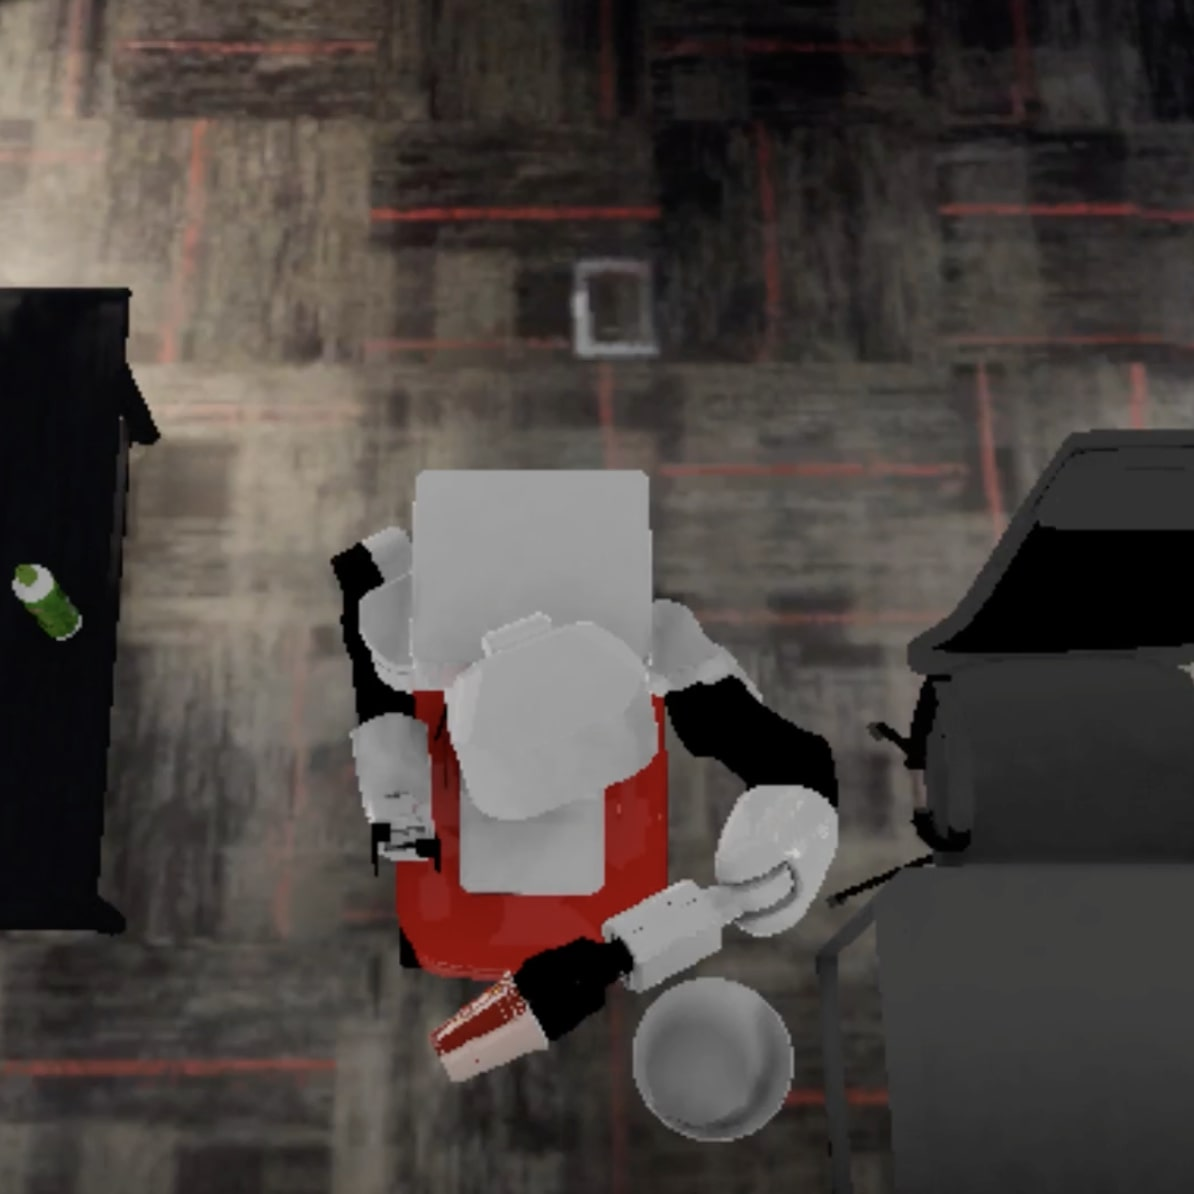
\includegraphics[trim=0 0 0 250,clip,width=0.3\linewidth]{figures/baseline_appendix/place_1}&
%         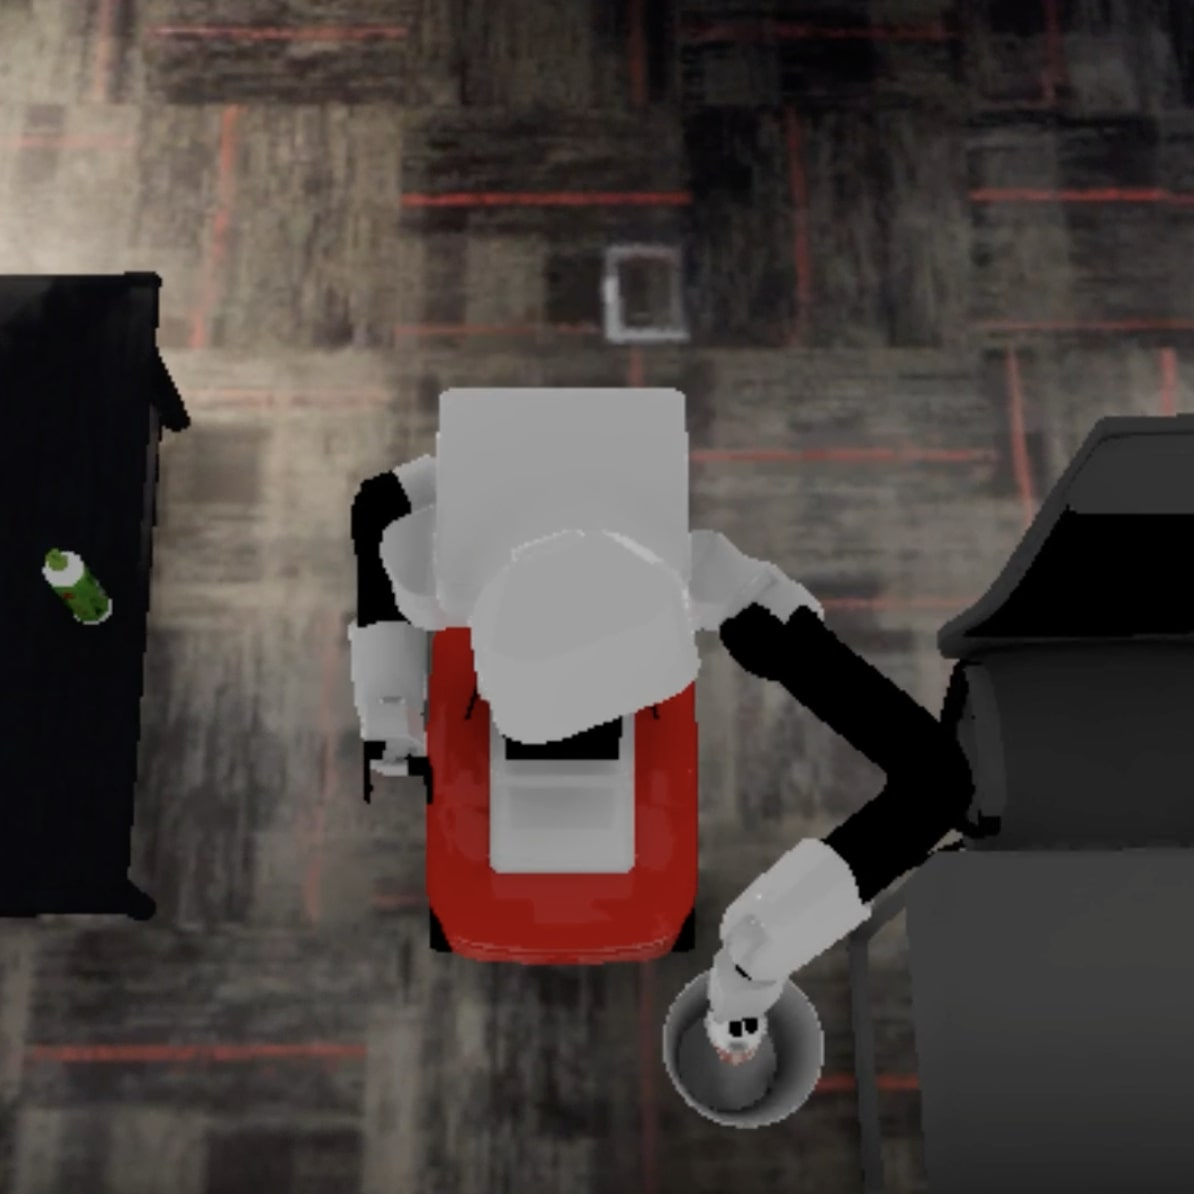
\includegraphics[trim=0 0 0 250,clip,width=0.3\linewidth]{figures/baseline_appendix/place_2}&
%         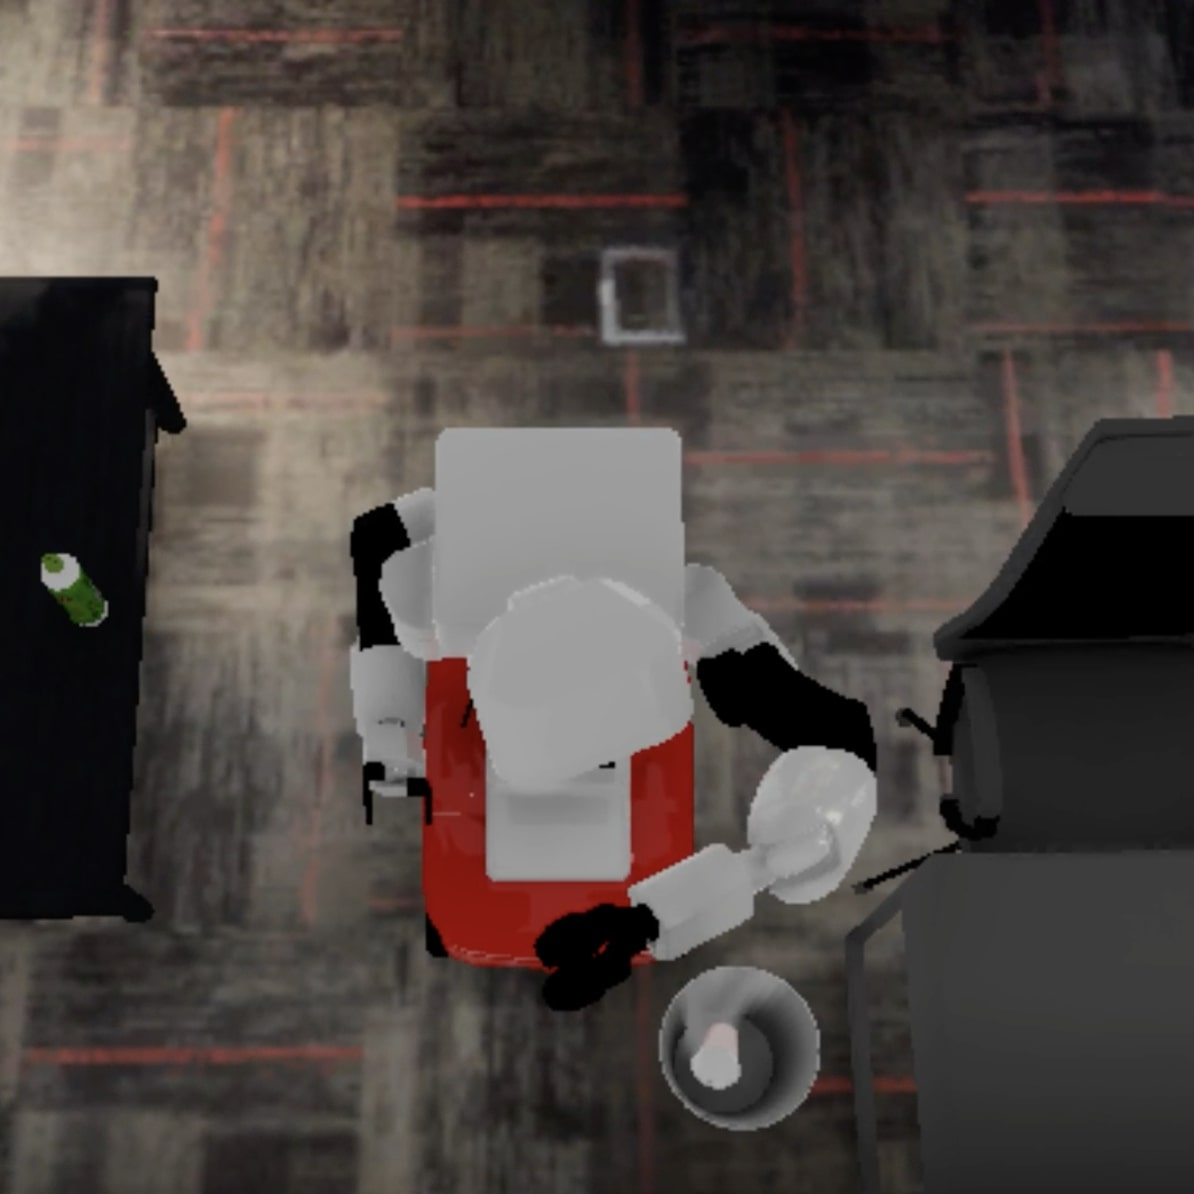
\includegraphics[trim=0 0 0 250,clip,width=0.3\linewidth]{figures/baseline_appendix/place_3}\\
%         & c) \texttt{place} & \\
%         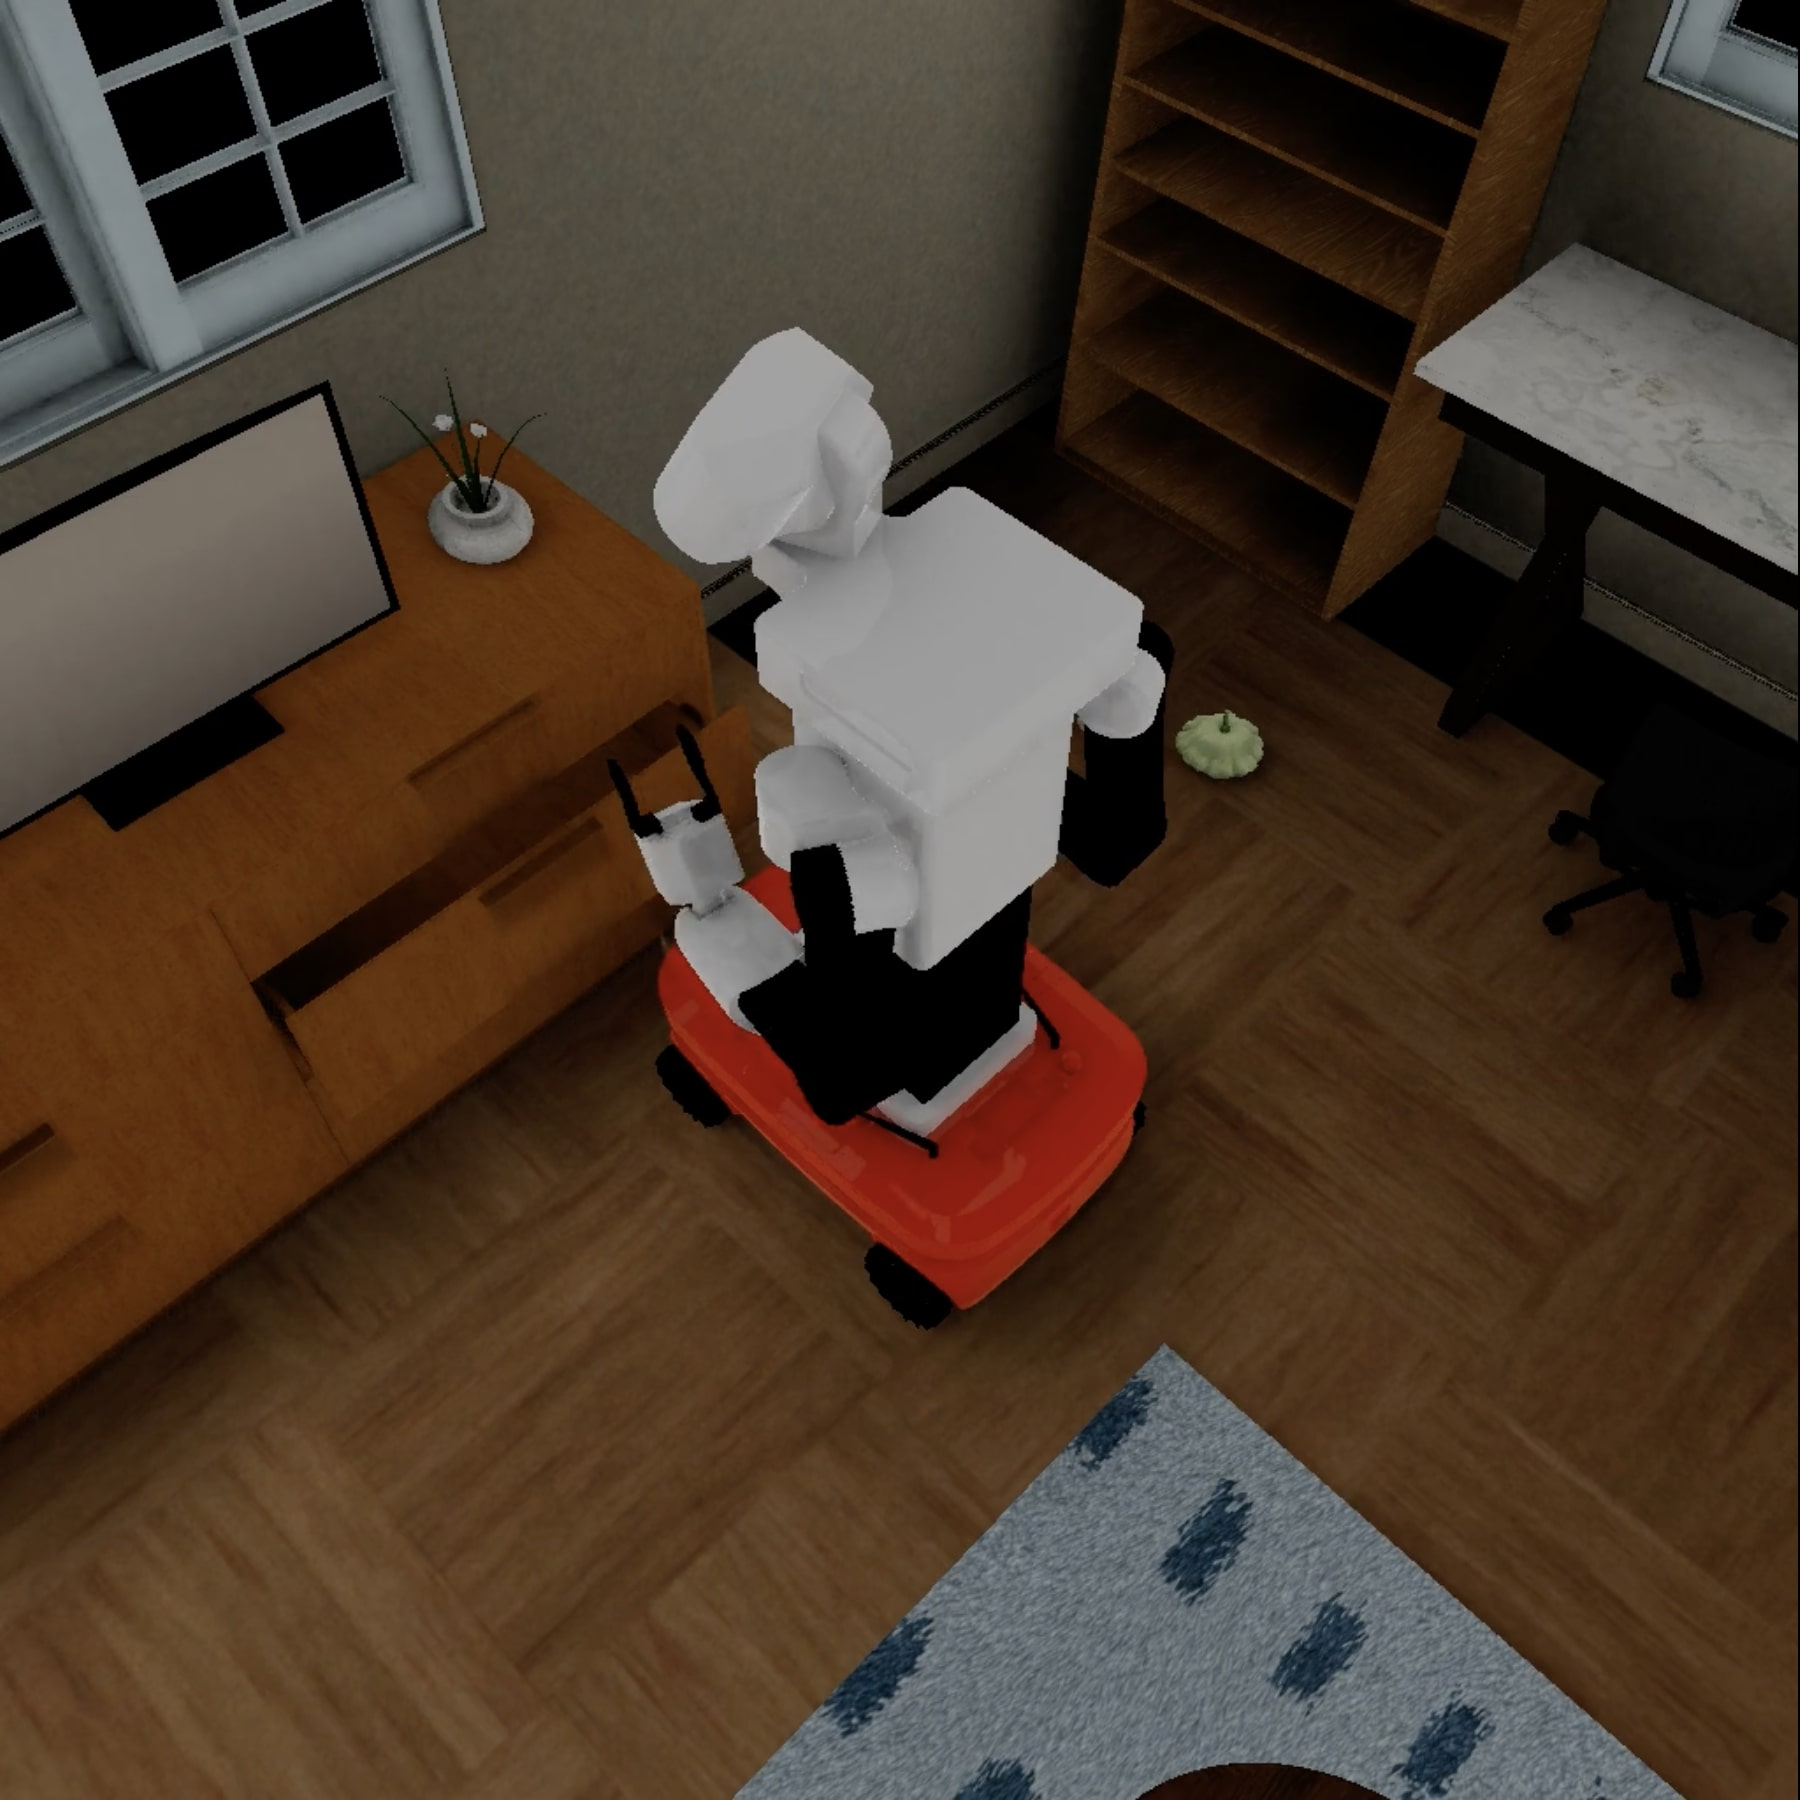
\includegraphics[trim=0 220 0 20,clip,width=0.3\linewidth]{figures/baseline_appendix/pull_1}&
%         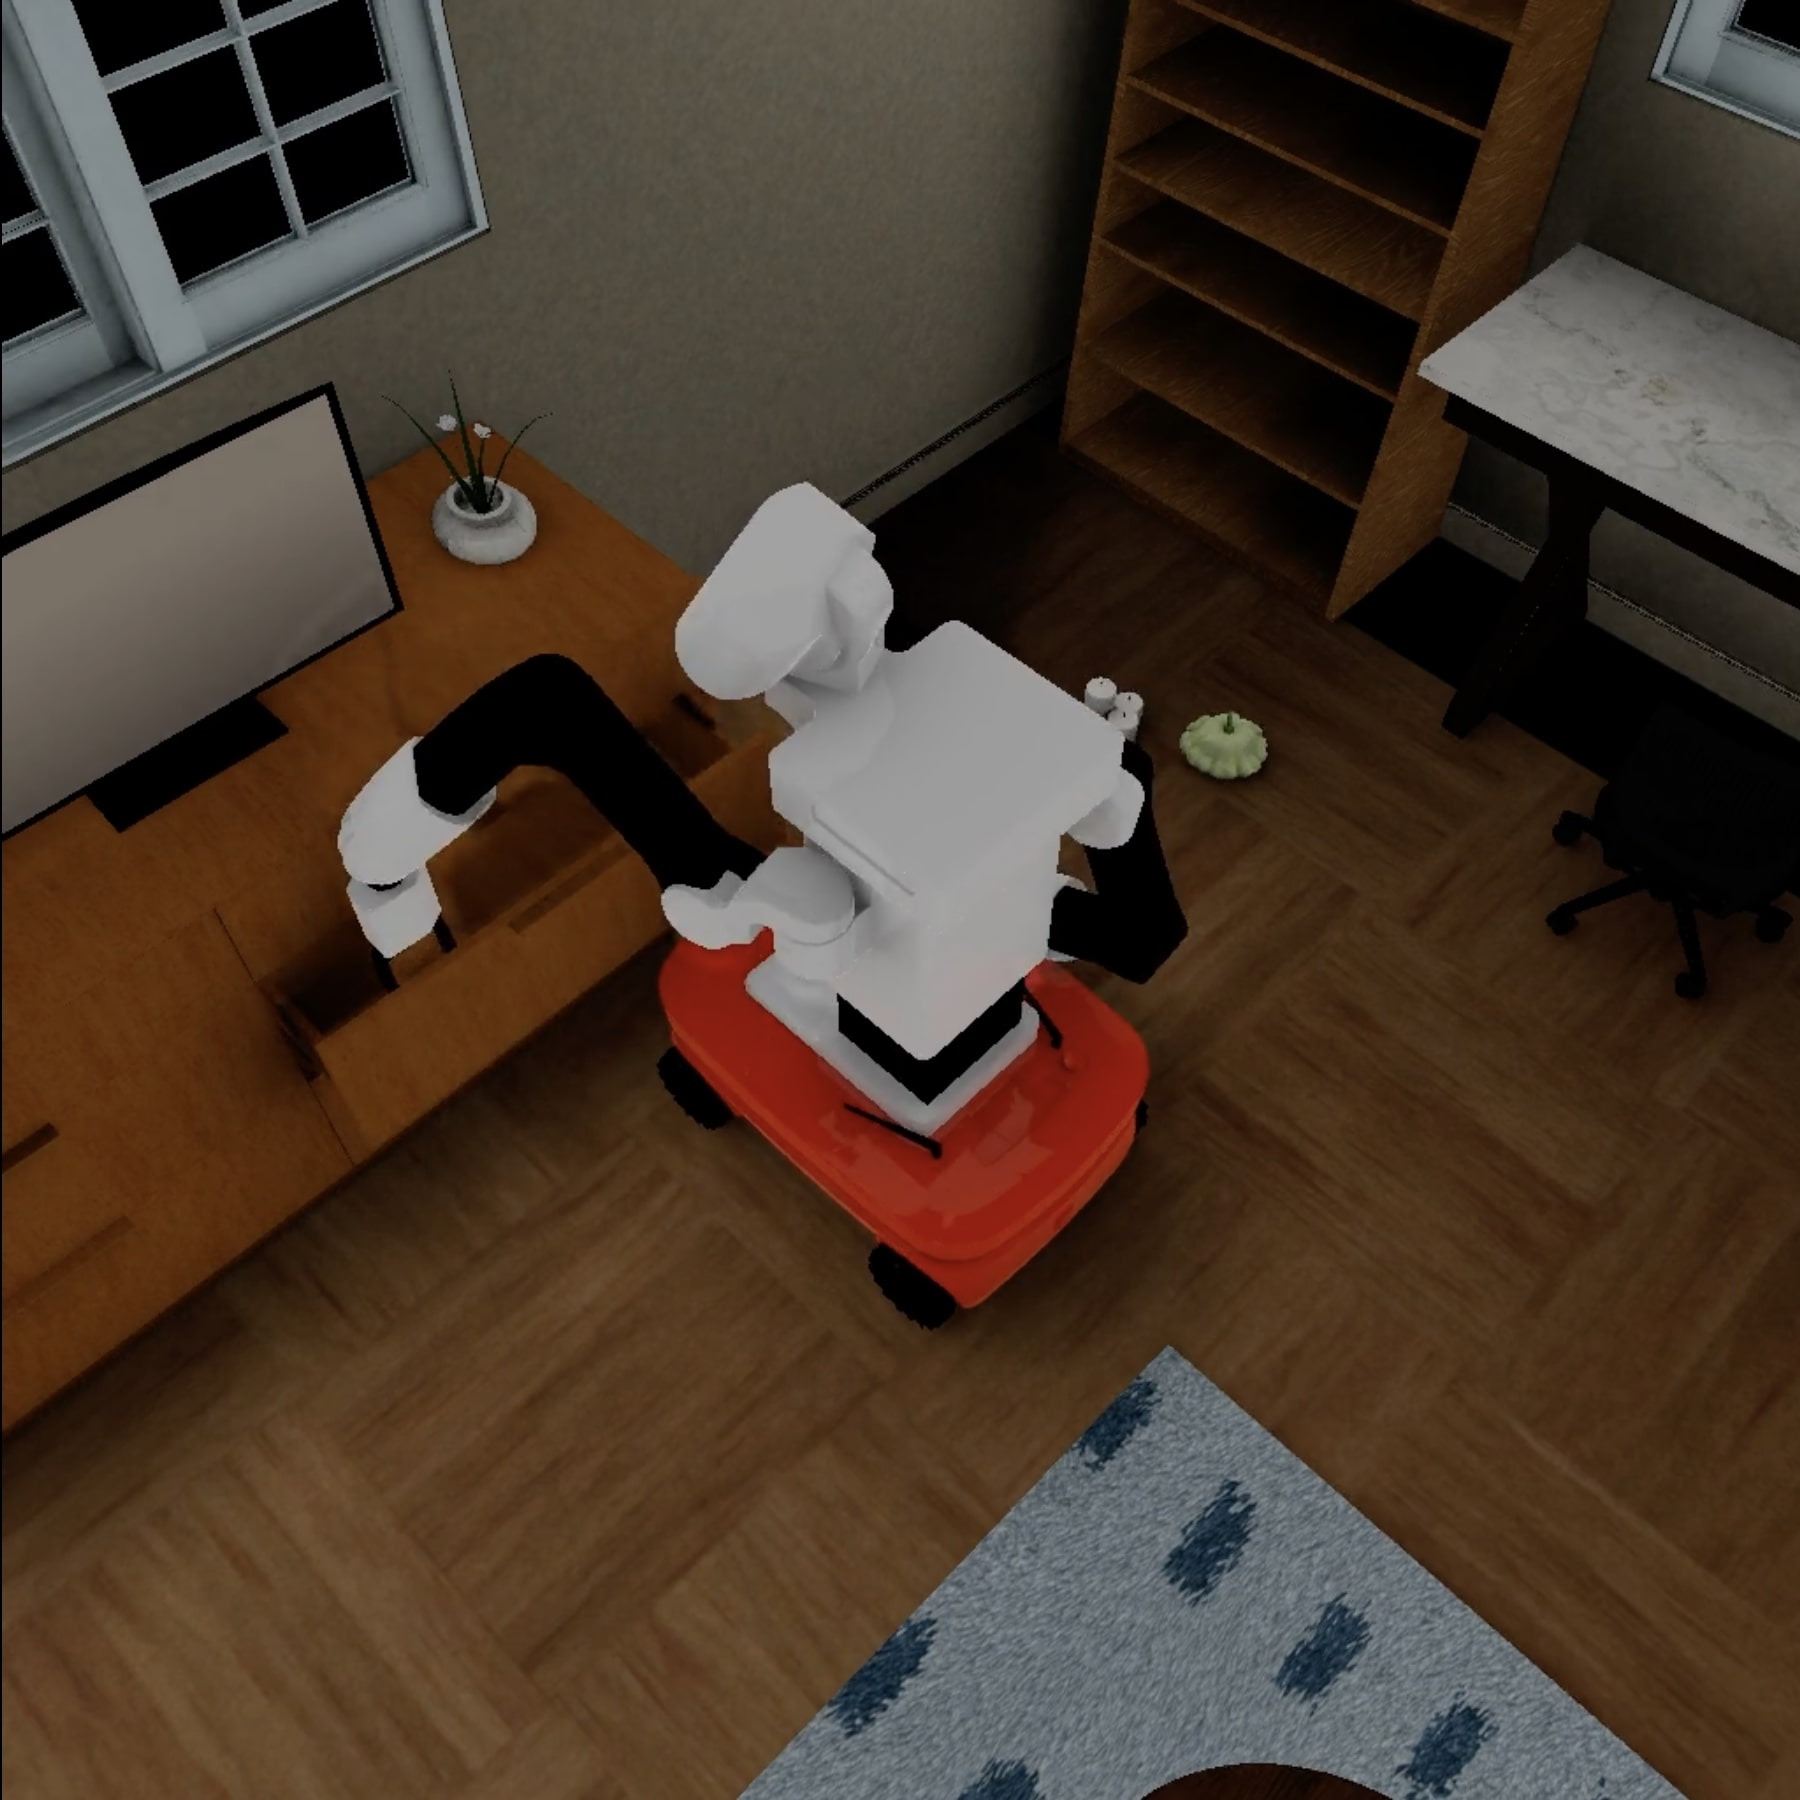
\includegraphics[trim=0 220 0 20,clip,width=0.3\linewidth]{figures/baseline_appendix/pull_2}&
%         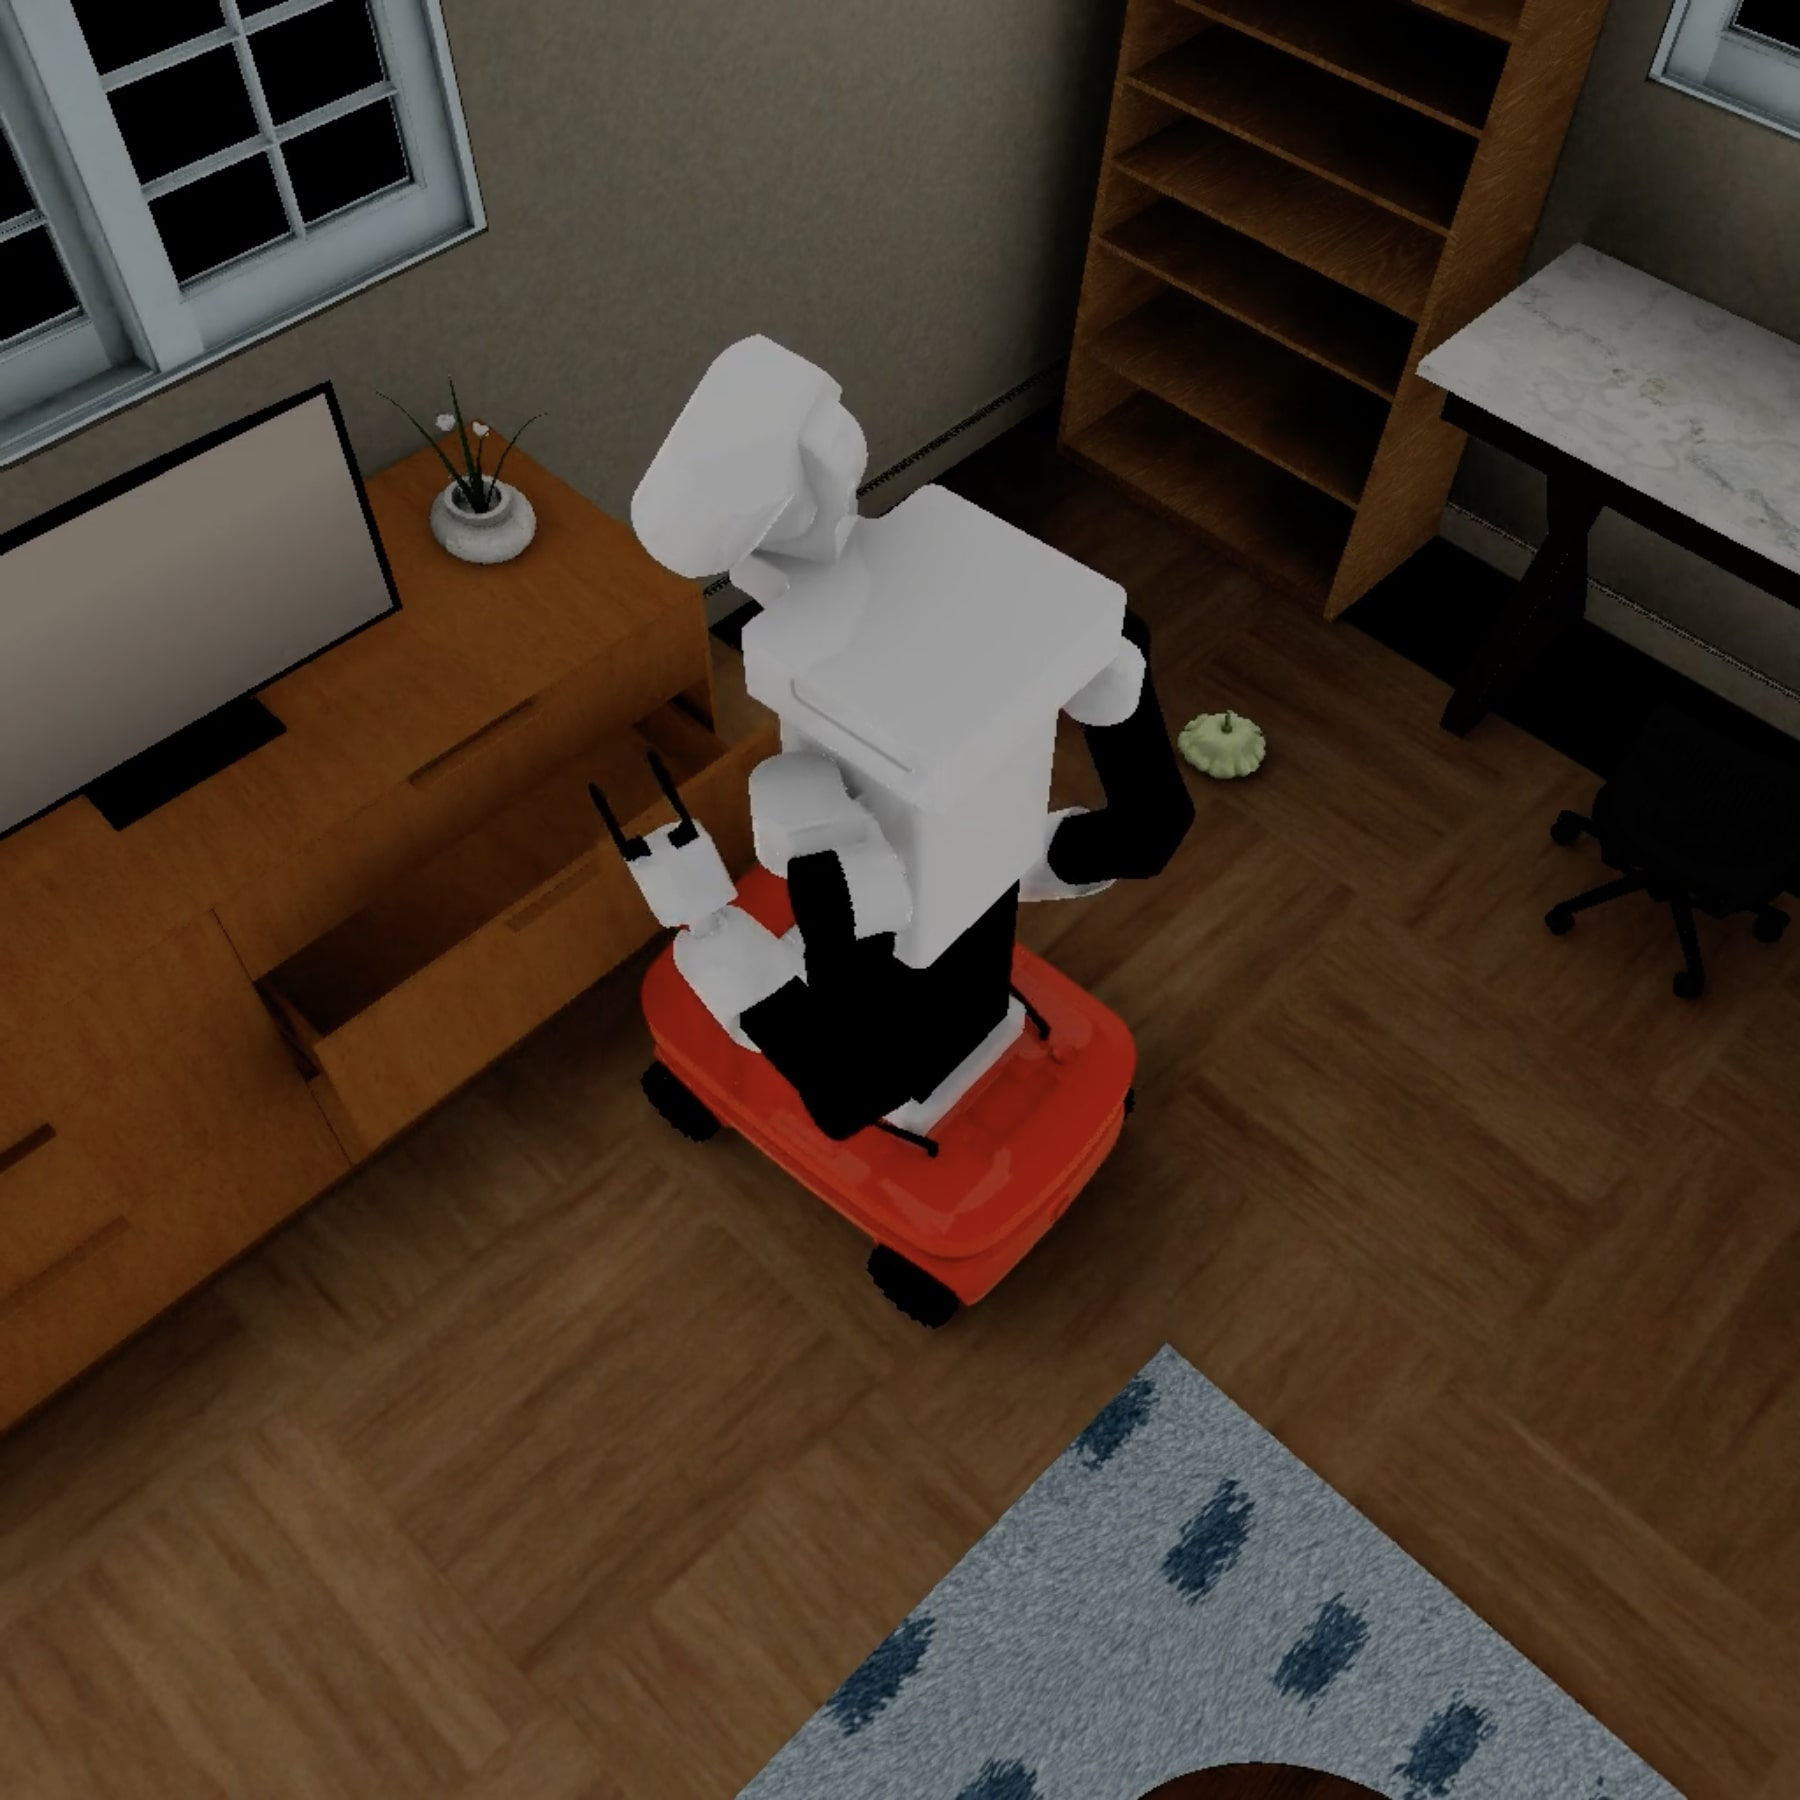
\includegraphics[trim=0 220 0 20,clip,width=0.3\linewidth]{figures/baseline_appendix/pull_3}\\
%         & d) \texttt{push} & \\
%         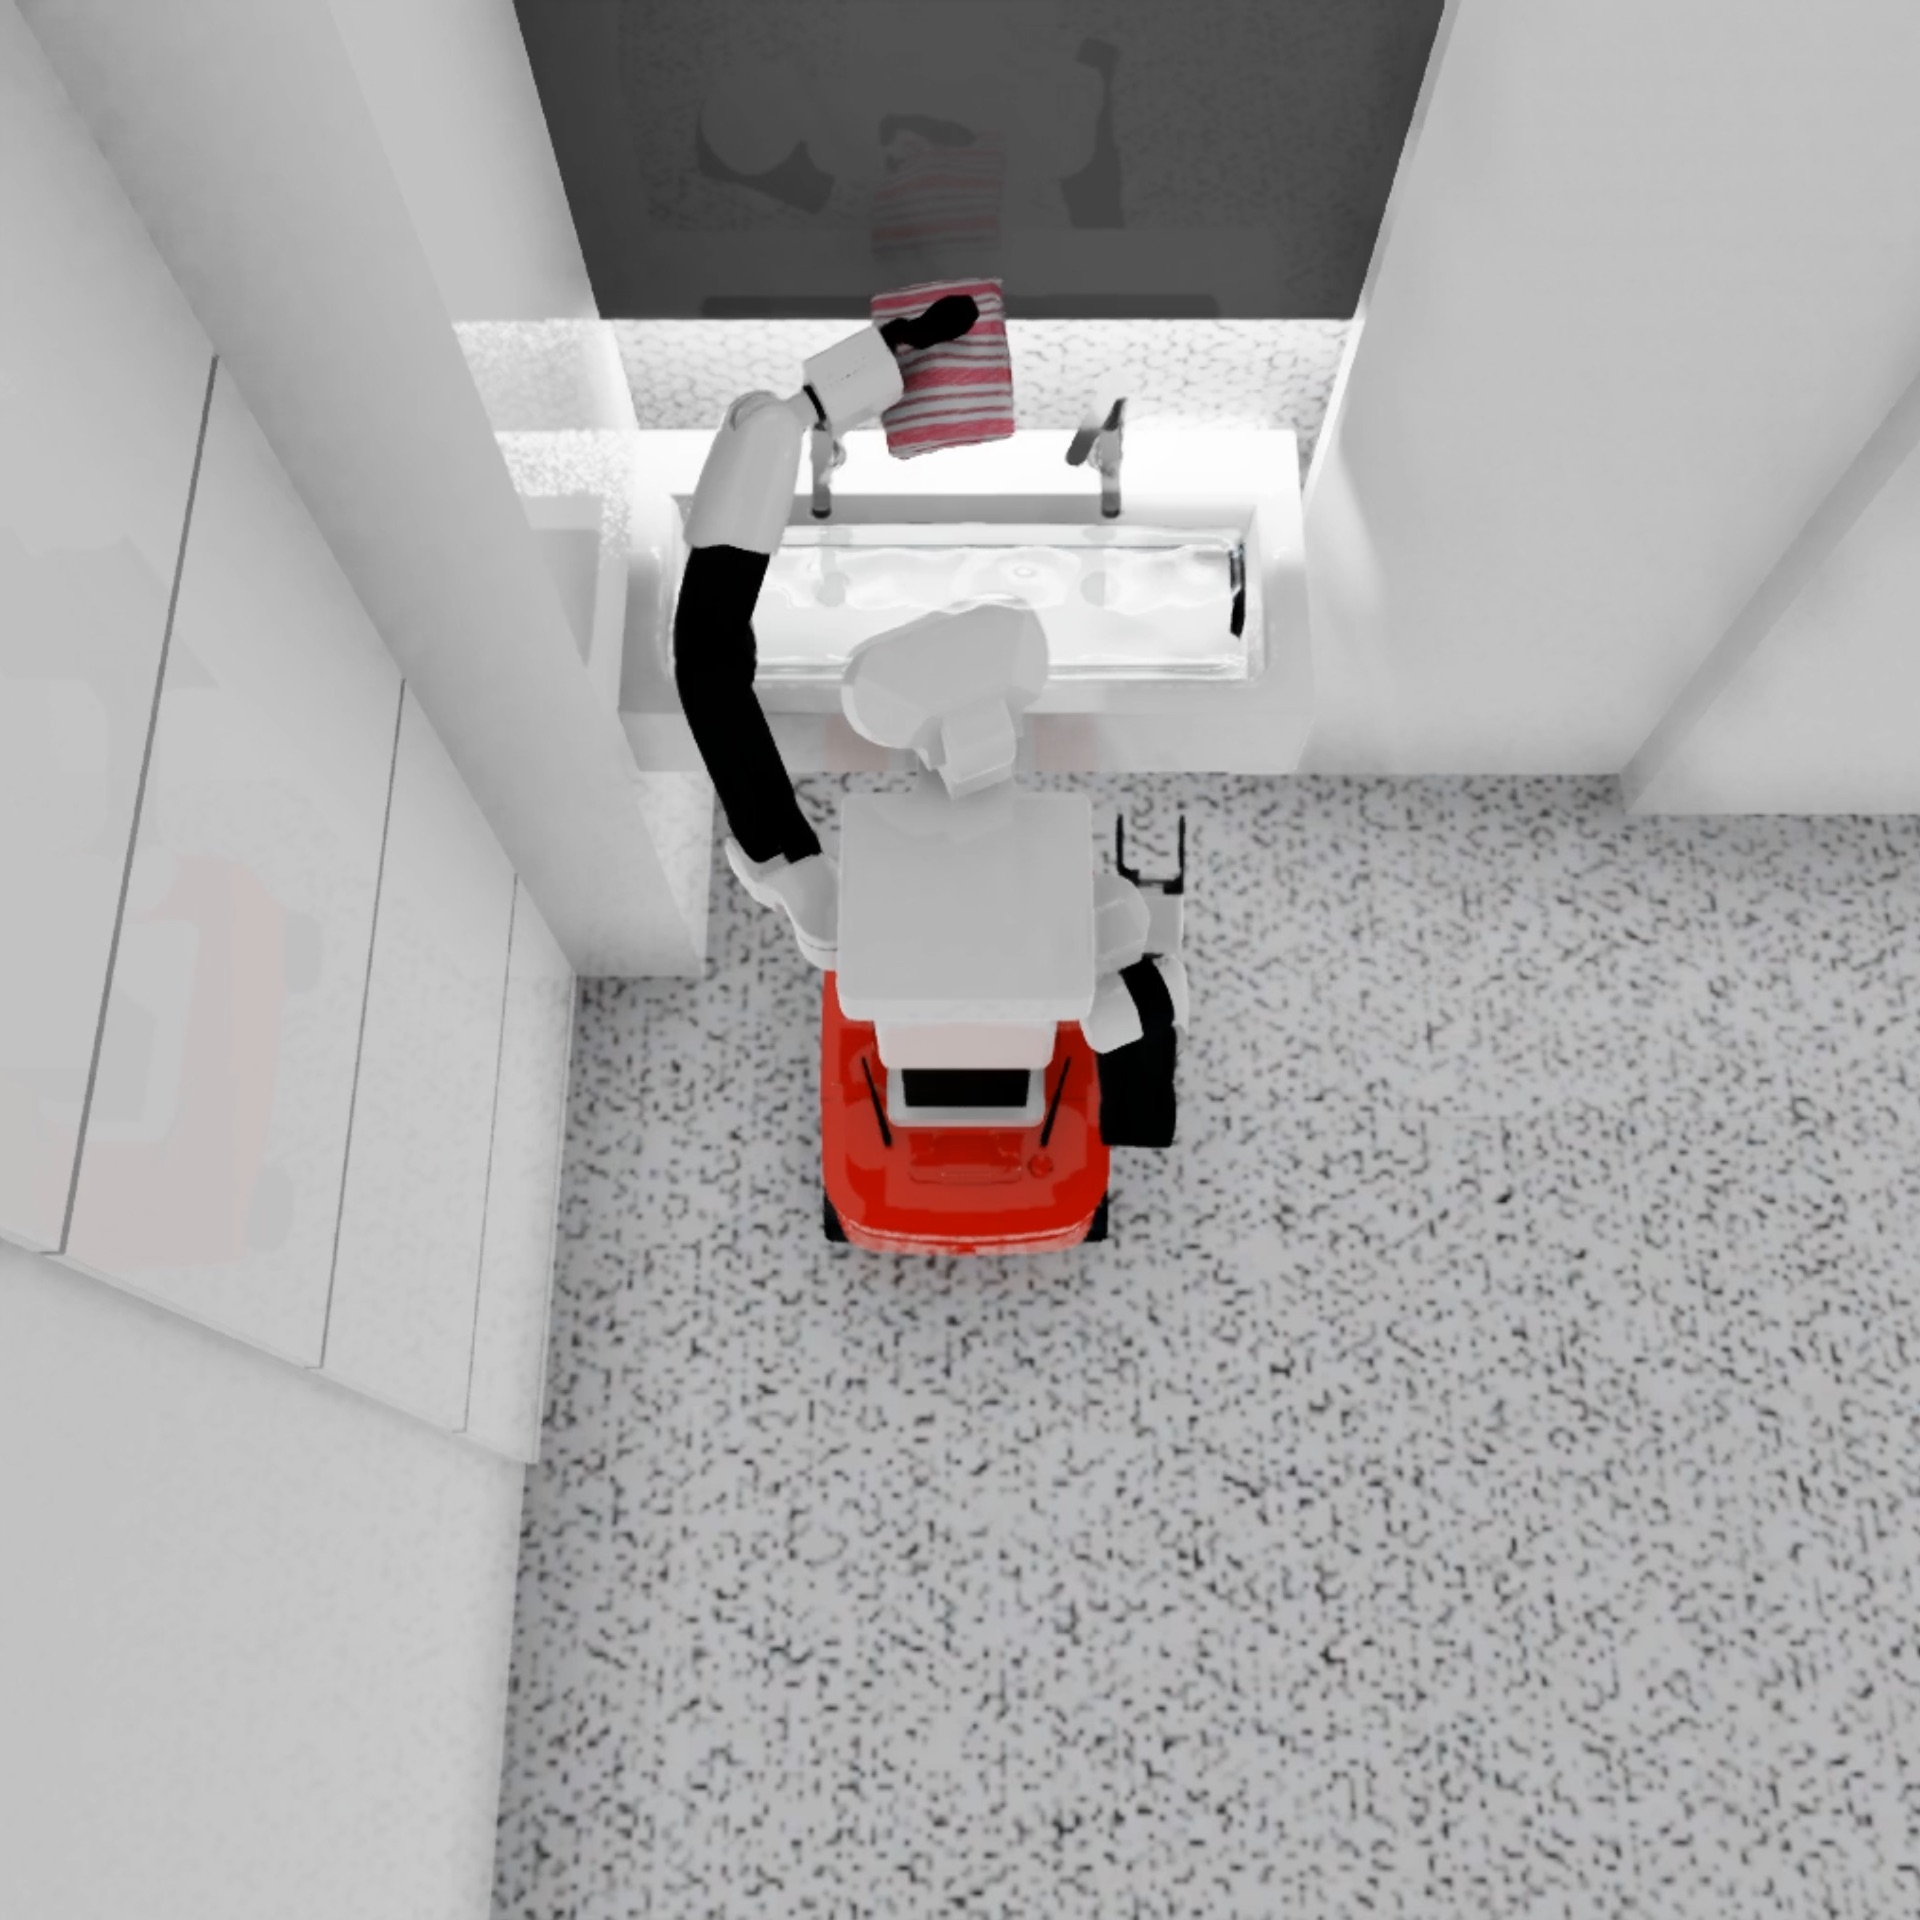
\includegraphics[trim=0 200 0 100,clip,width=0.3\linewidth]{figures/baseline_appendix/dip_1}&
%         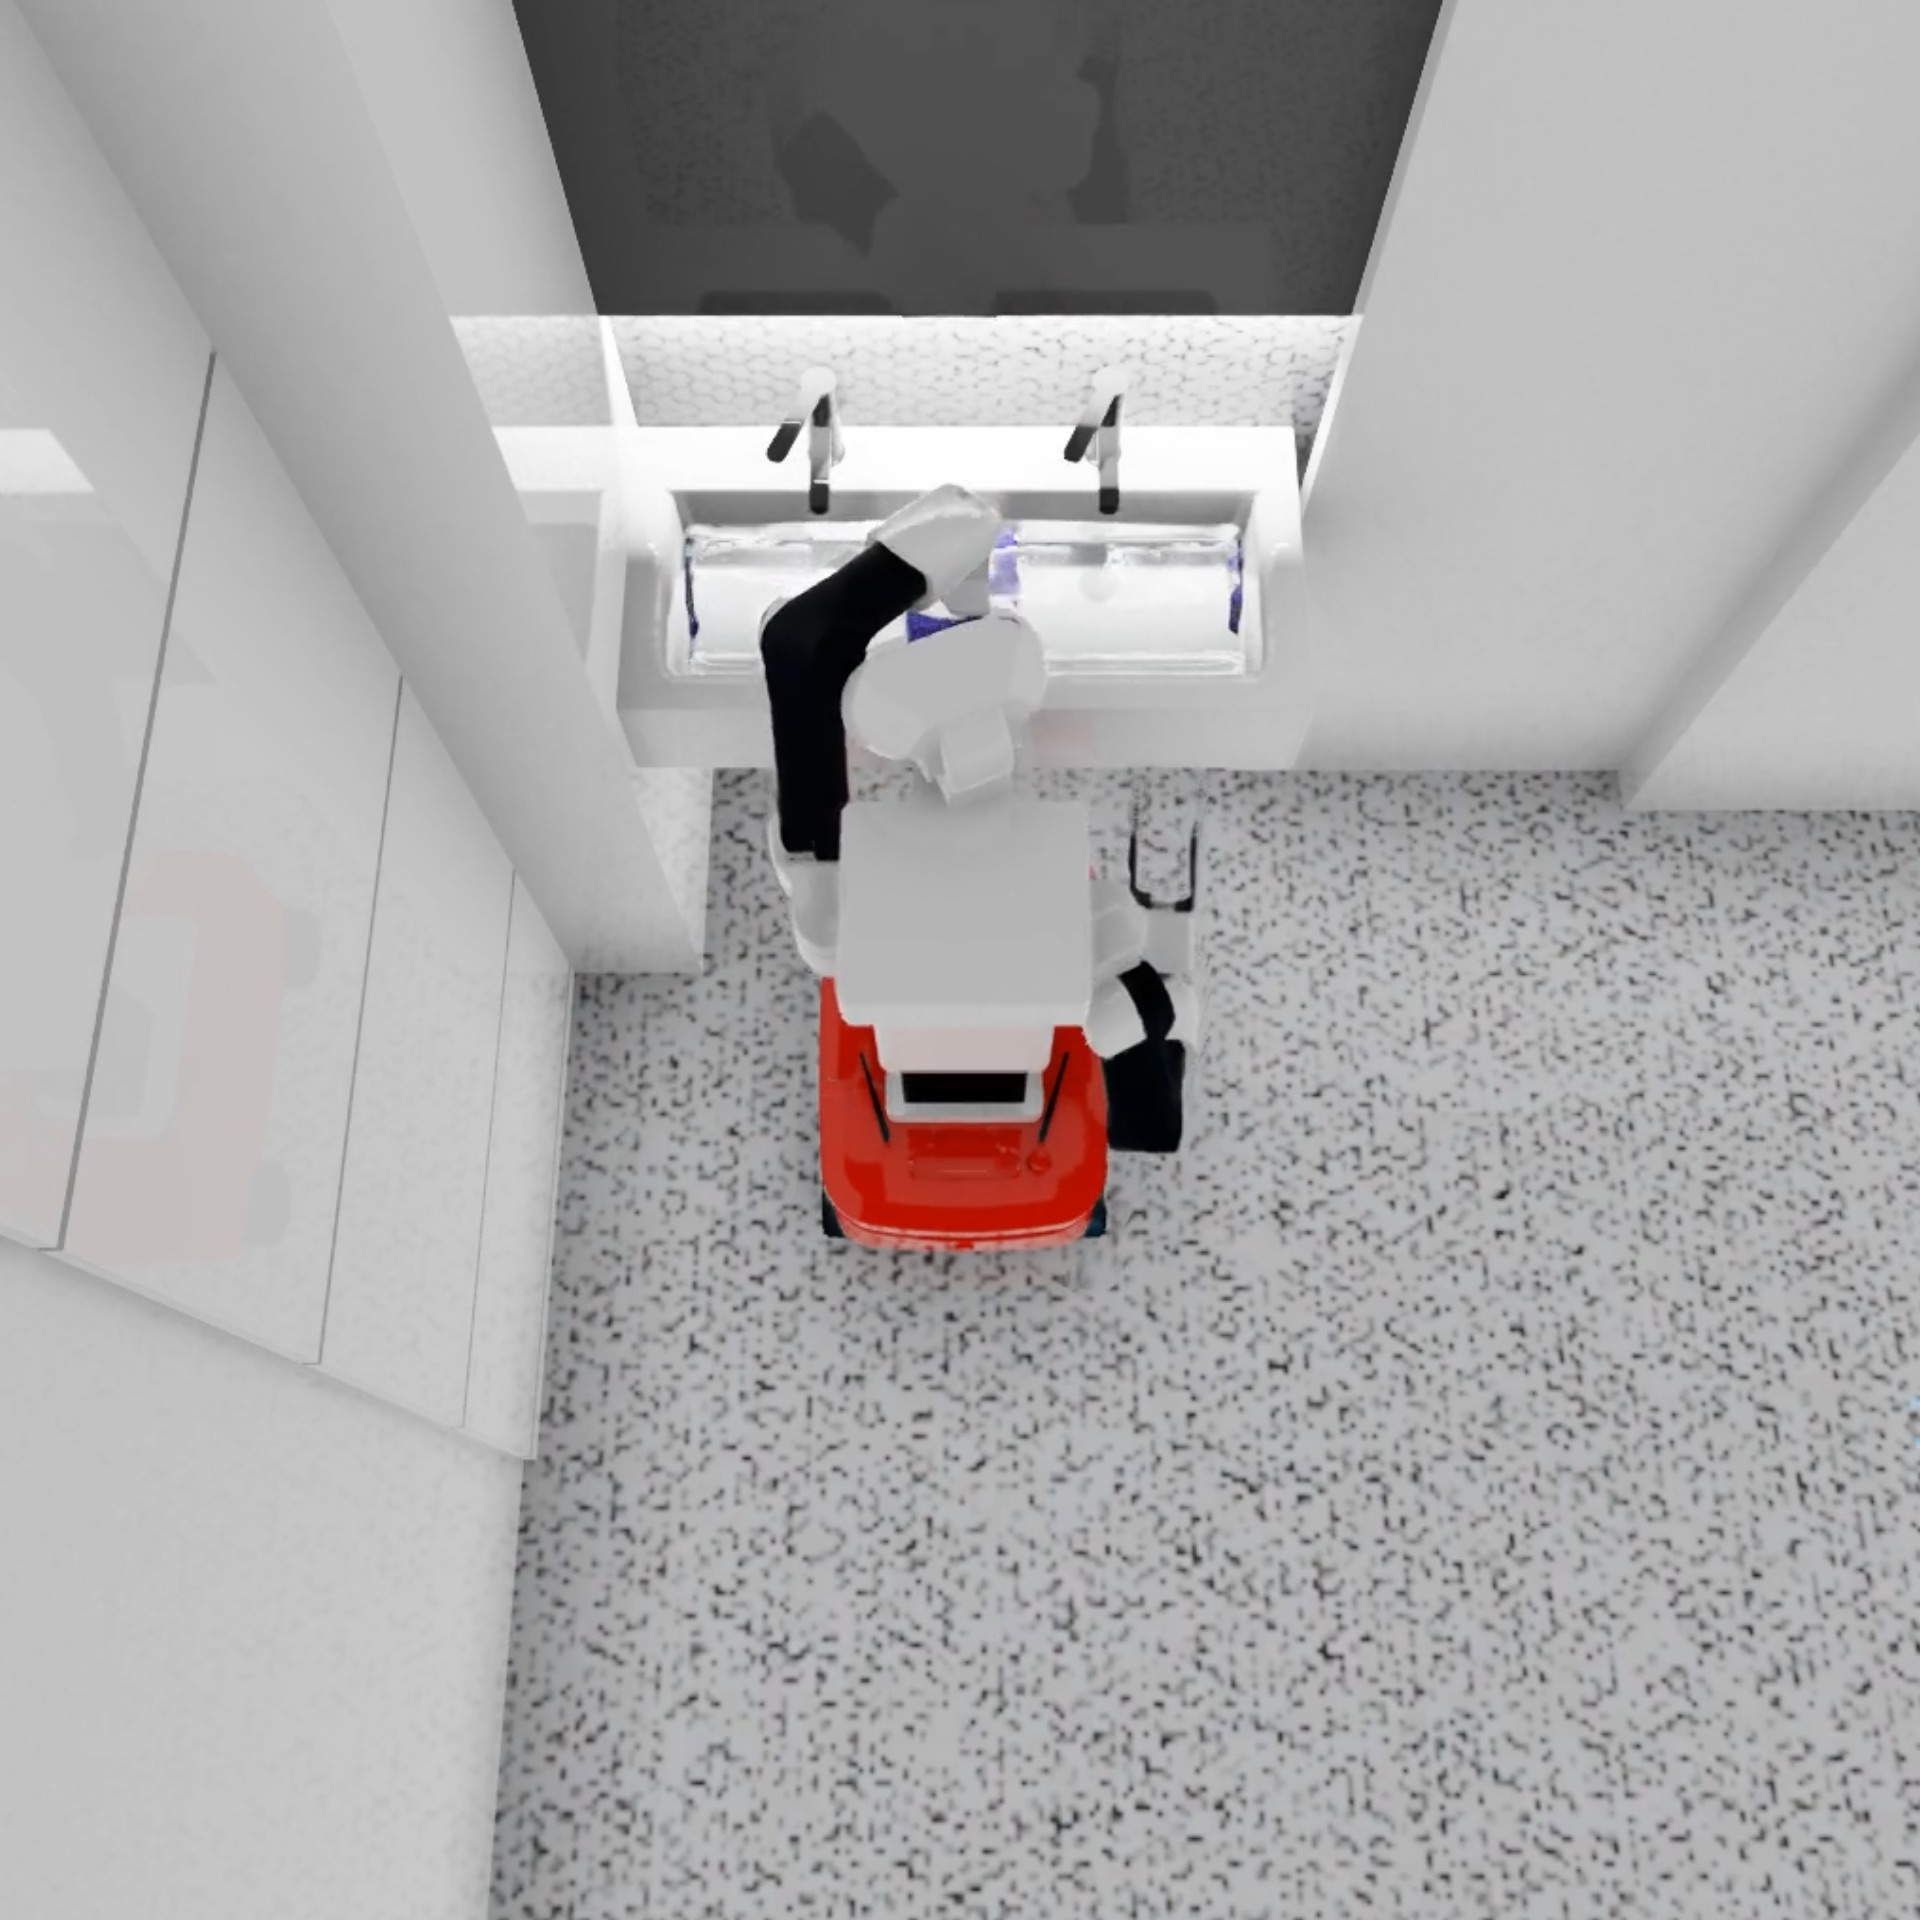
\includegraphics[trim=0 200 0 100,clip,width=0.3\linewidth]{figures/baseline_appendix/dip_2}&
%         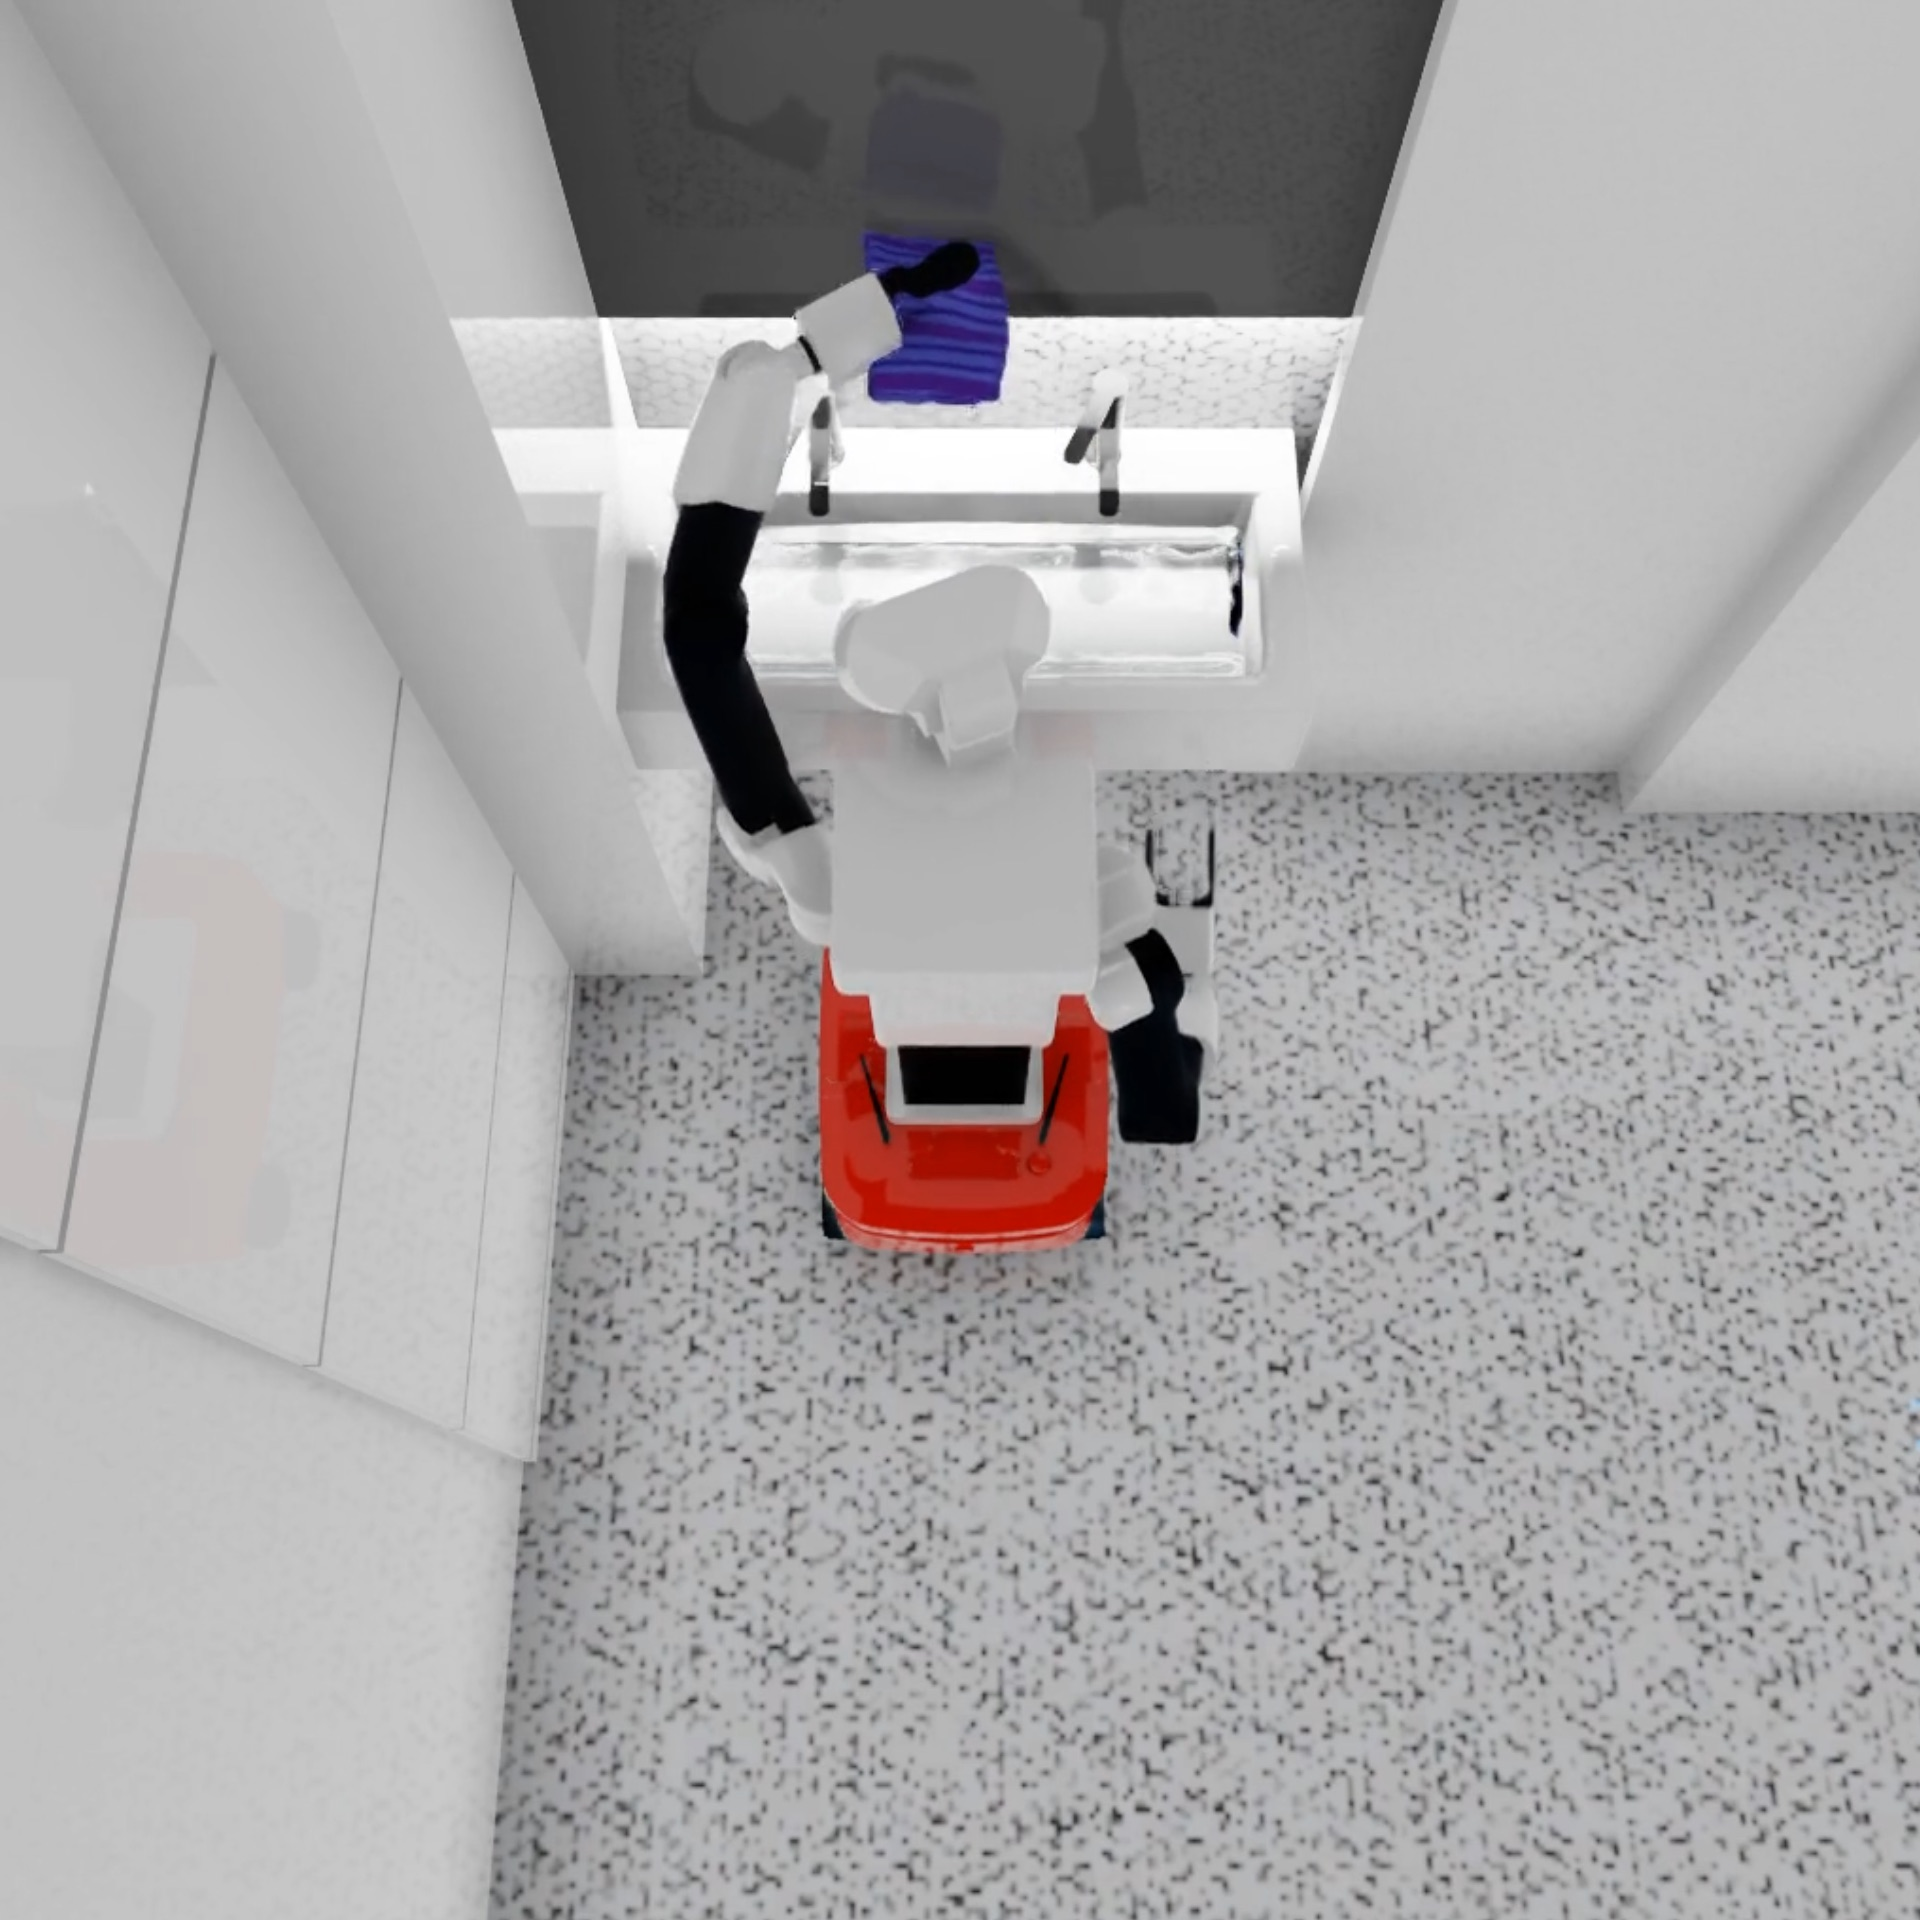
\includegraphics[trim=0 200 0 100,clip,width=0.3\linewidth]{figures/baseline_appendix/dip_3}\\
%         & e) \texttt{dip}  & \\
%         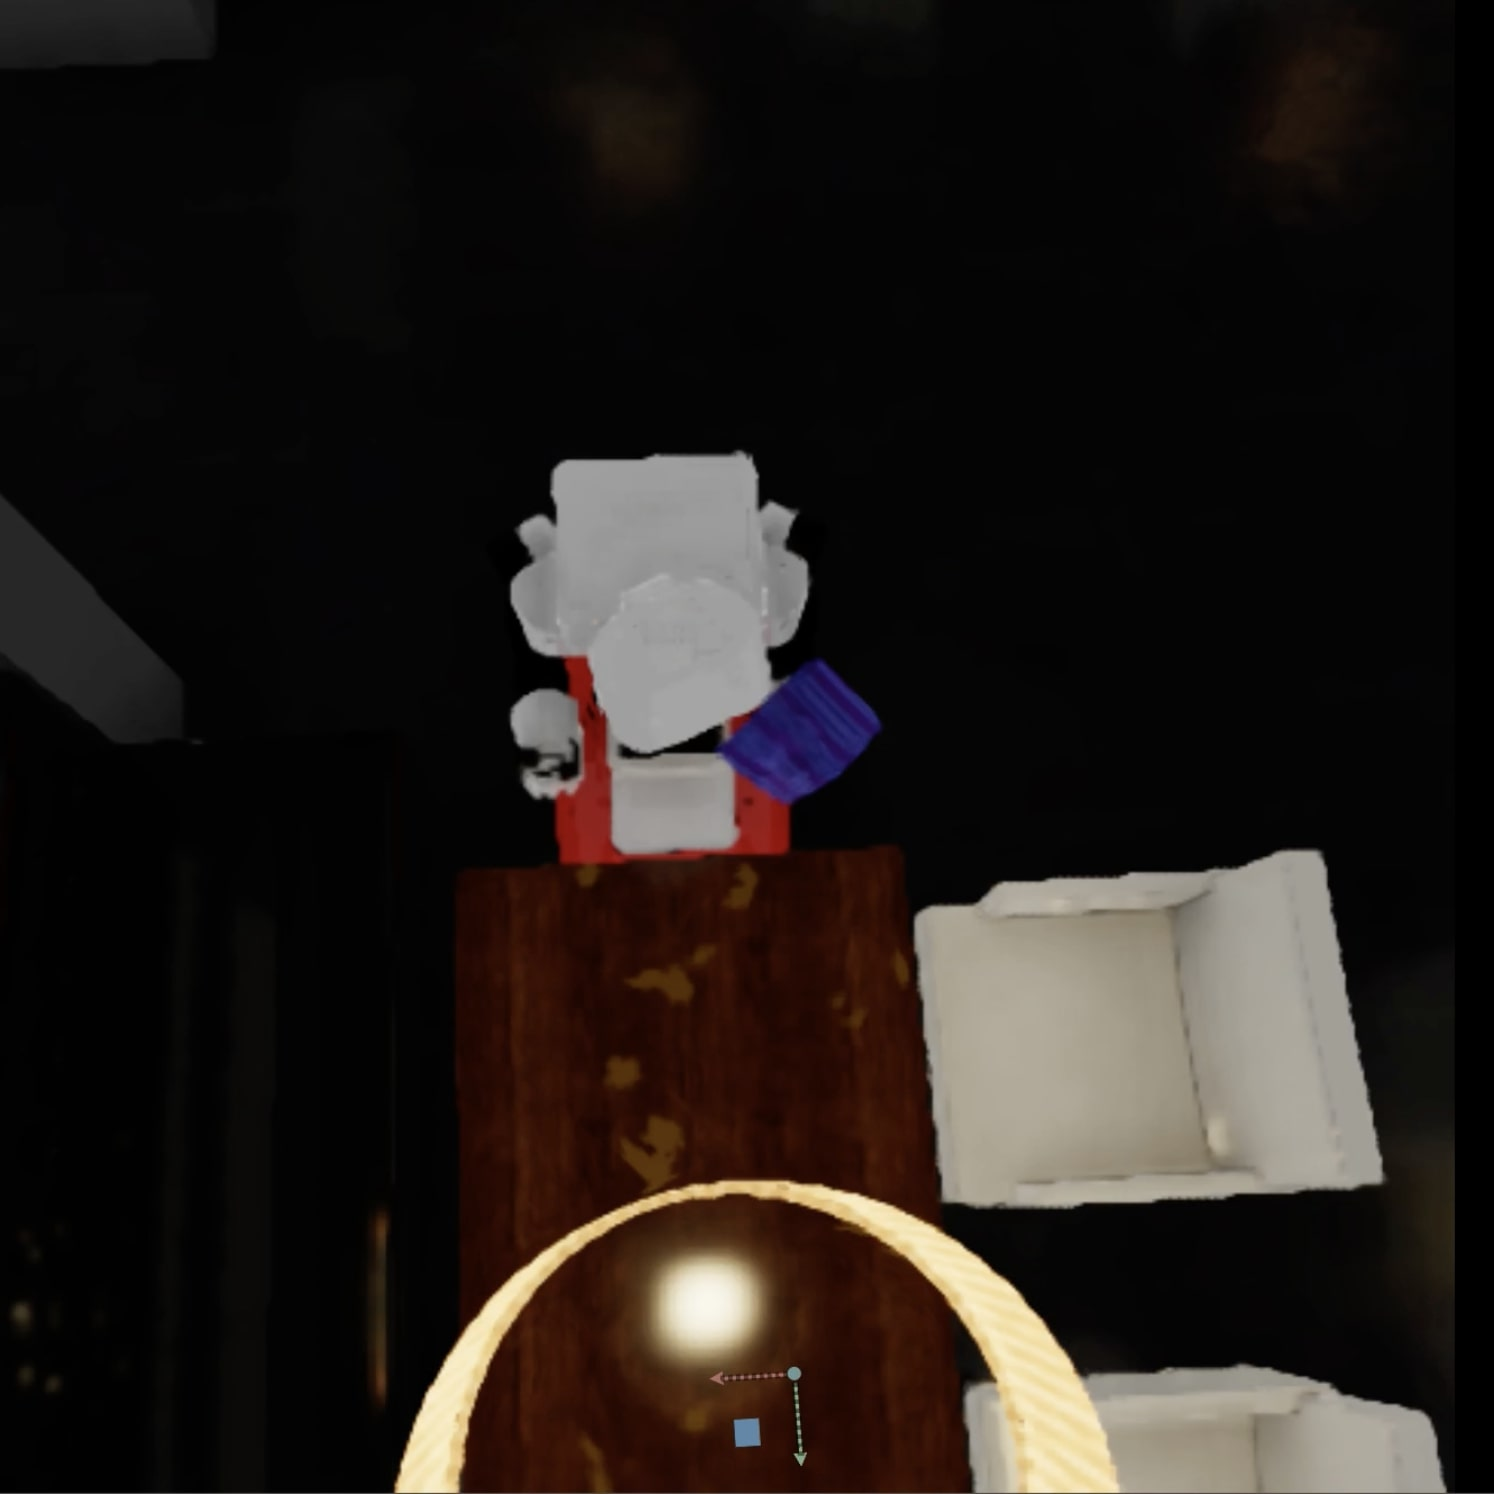
\includegraphics[trim=0 100 0 200,clip,width=0.3\linewidth]{figures/baseline_appendix/wipe_1}&
%         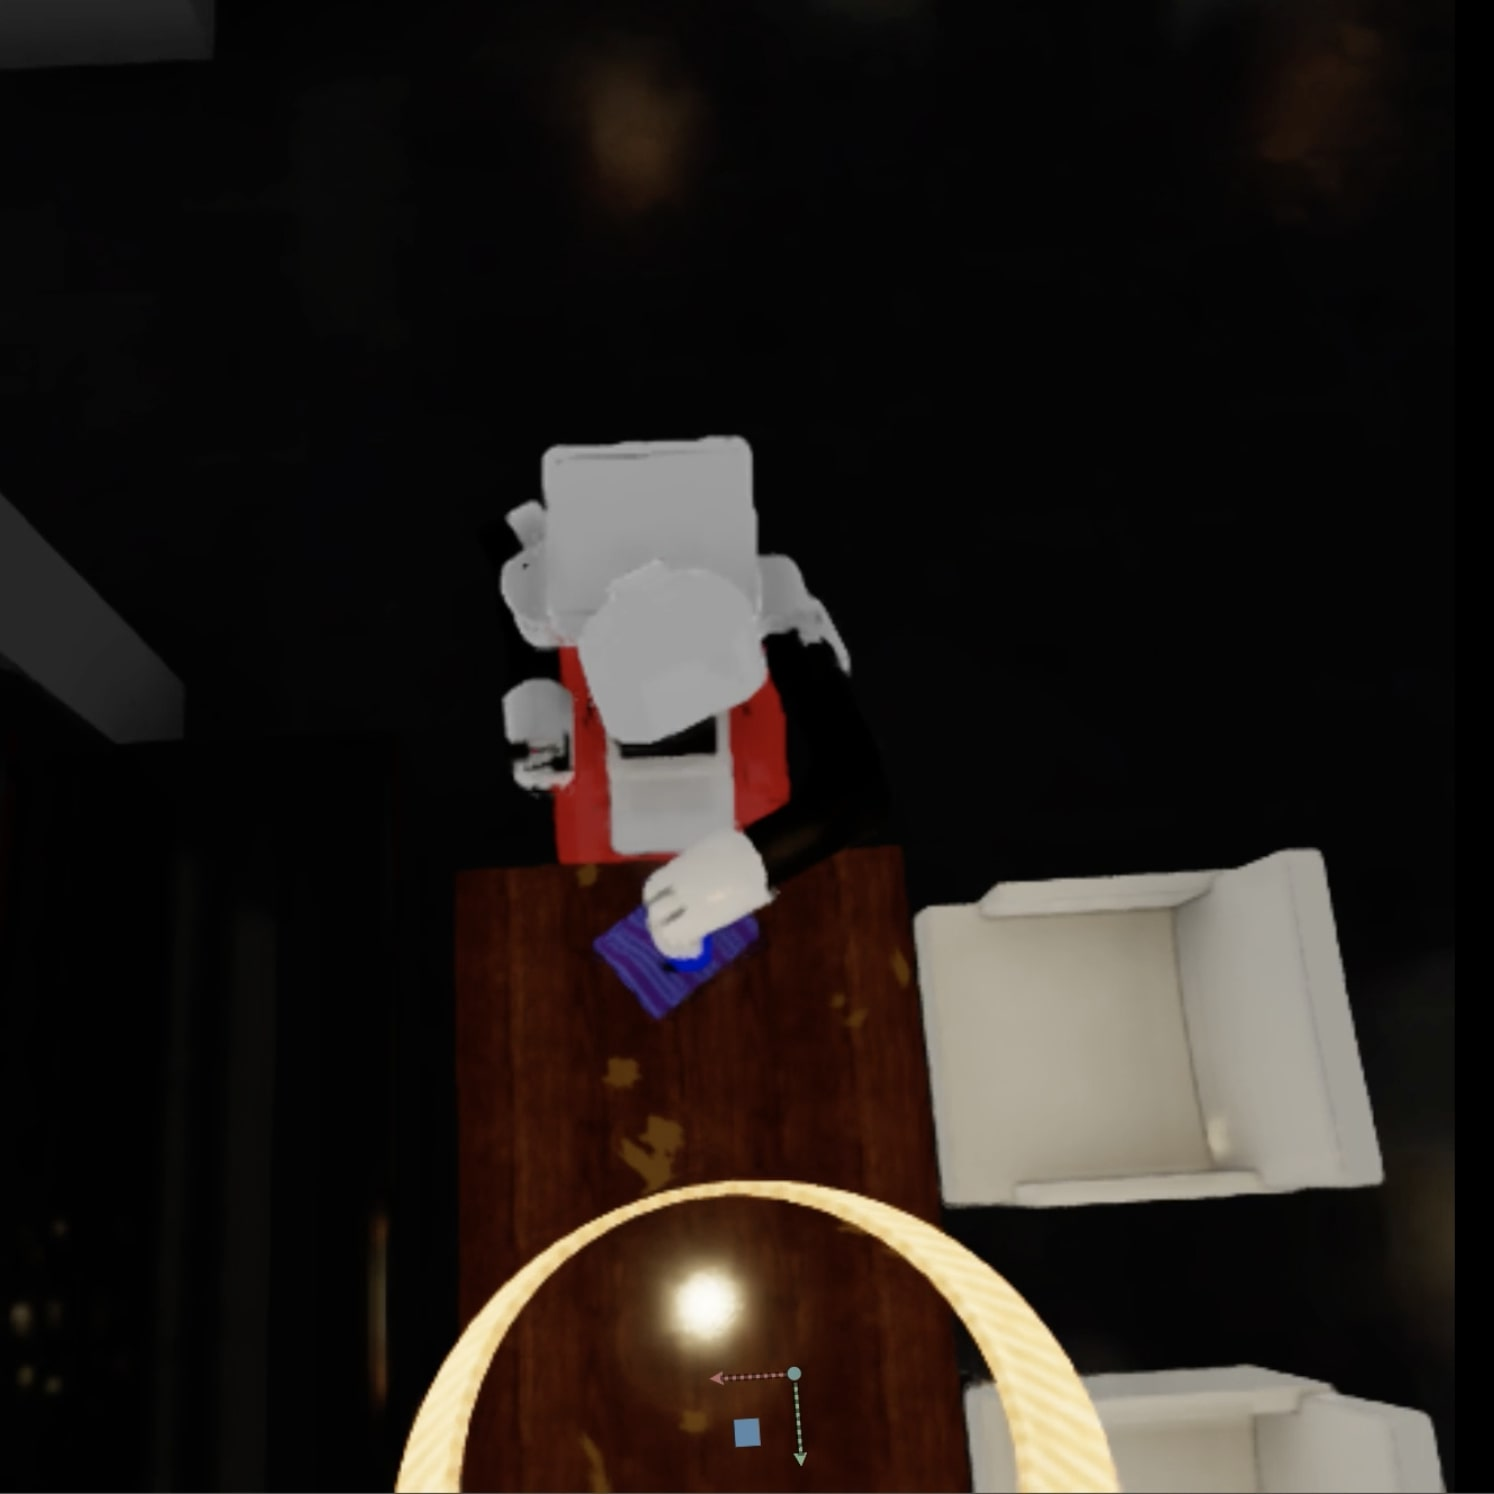
\includegraphics[trim=0 100 0 200,clip,width=0.3\linewidth]{figures/baseline_appendix/wipe_2}&
%         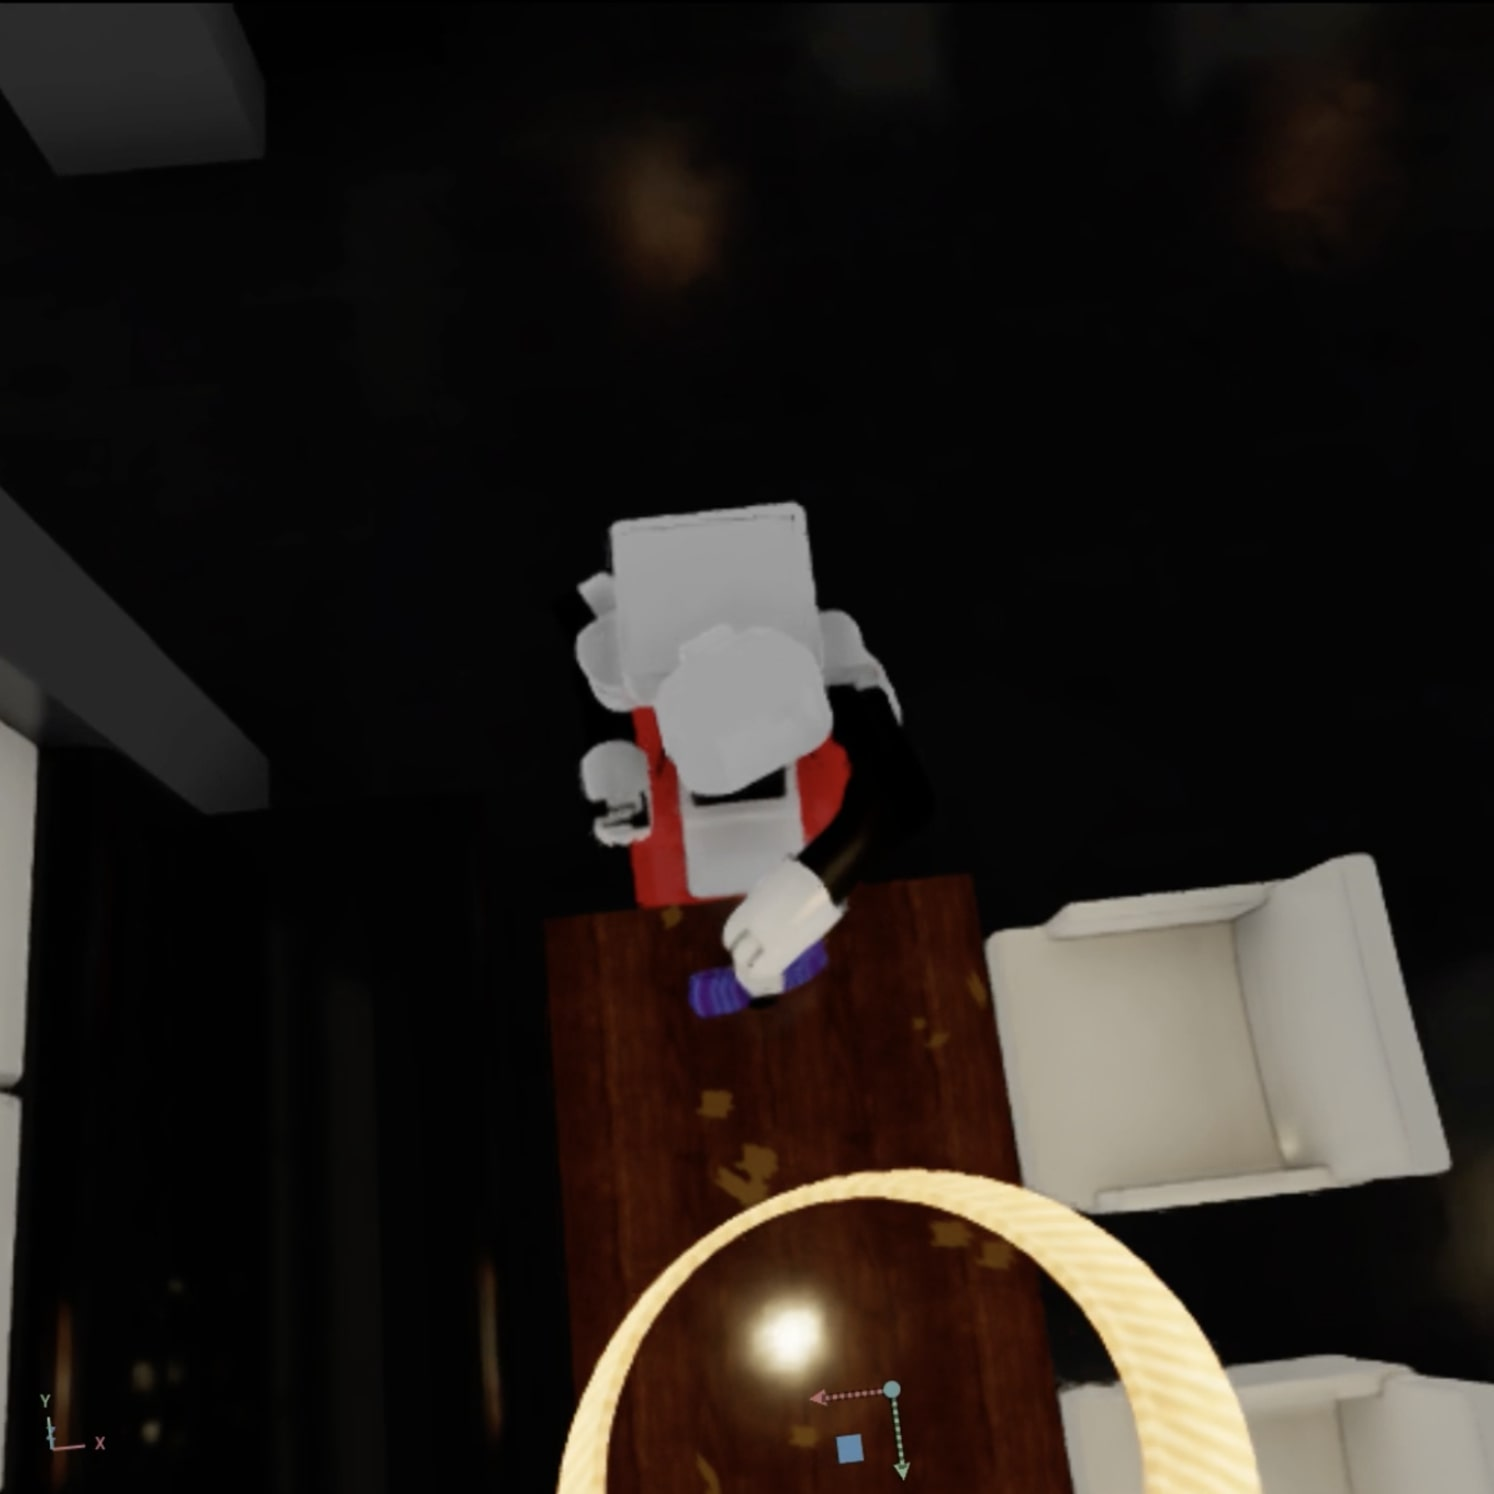
\includegraphics[trim=0 100 0 200,clip,width=0.3\linewidth]{figures/baseline_appendix/wipe_3}\\
%         & f) \texttt{wipe}  & \\
%     \end{tabular}
%     \caption{Overview of all the high level planner actions with the pre-conditions (right), post-conditions (left), and an intermediate state when executing the action.
%     % \roberto{consider taking the images of wipe with more lights, it is hard to see. and the robot is gone in the last image}
%     }
%     \label{fig:appendix_high_level_planner}
% \end{figure}

\begin{figure}[h!]
\centering
\begin{subfigure}[t]{0.8\textwidth}{\centering
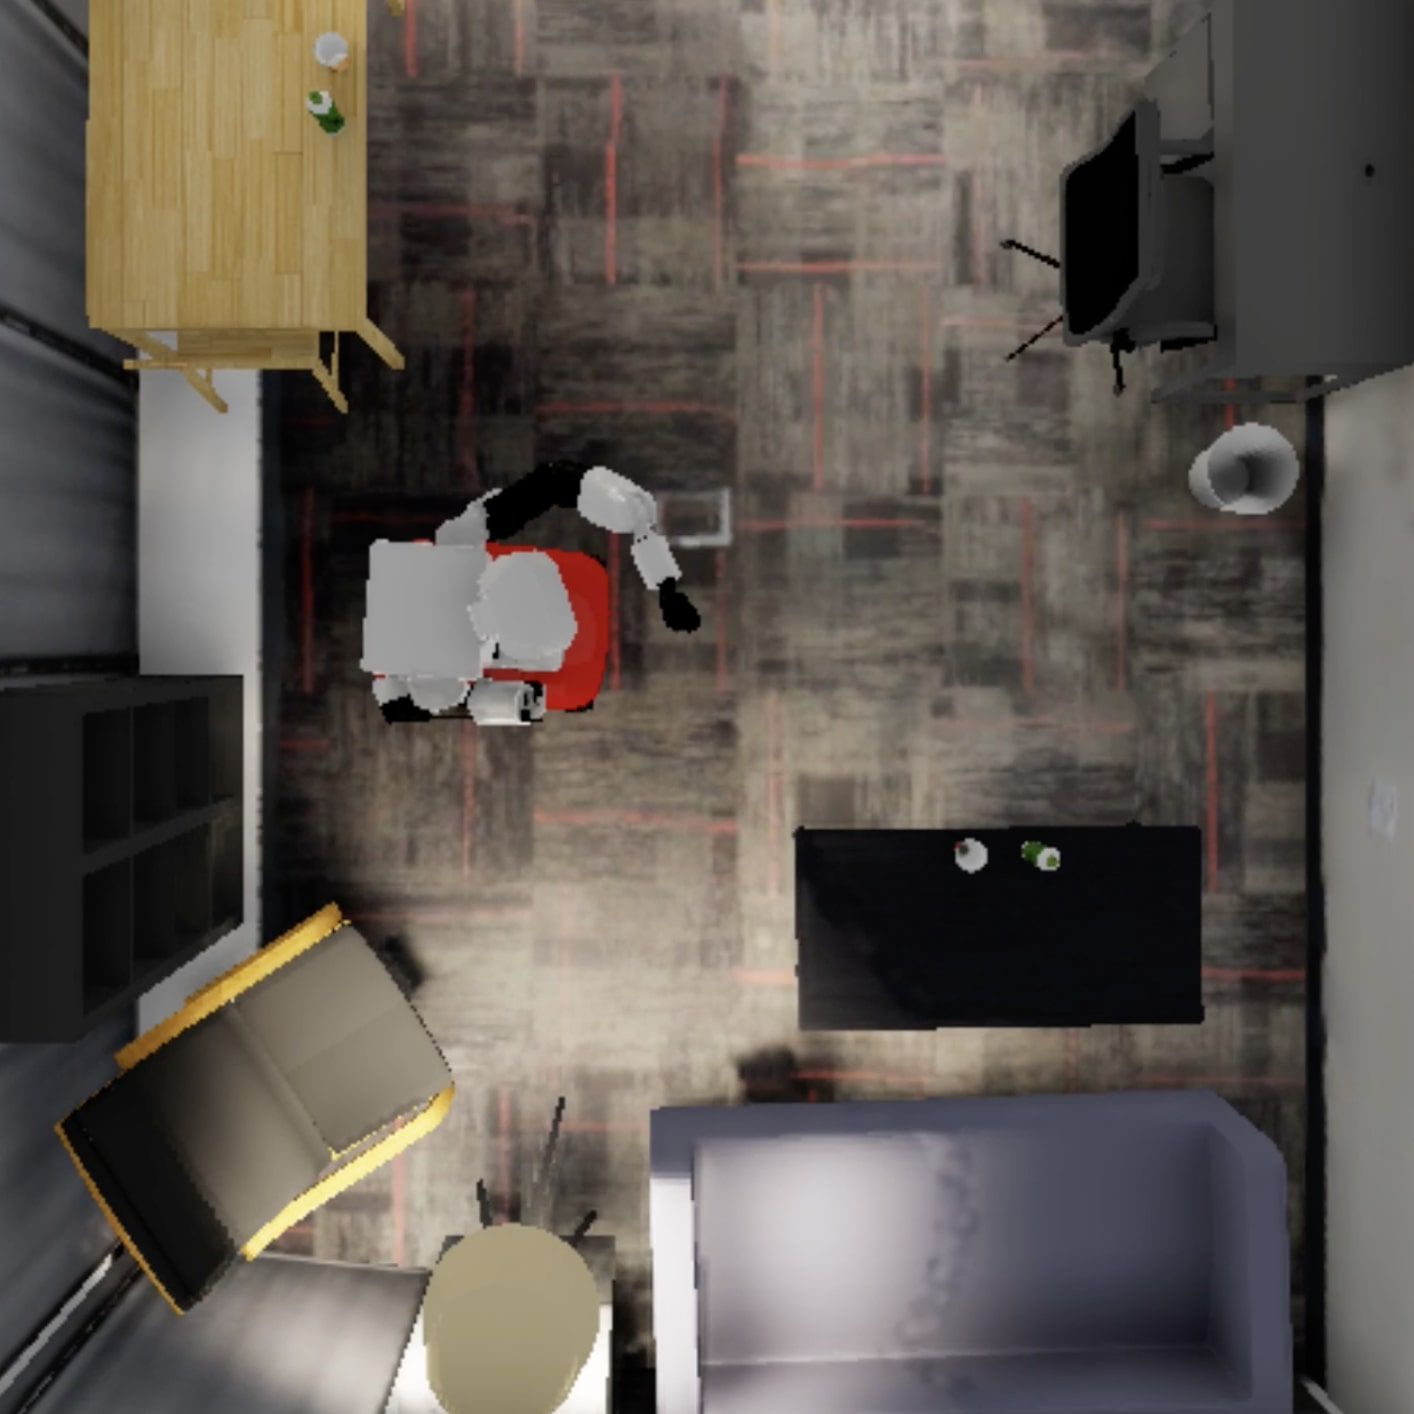
\includegraphics[trim=0 200 0 200,clip,width=0.33\linewidth]{figures/baseline_appendix/navigate_to_1}%
\hfill%
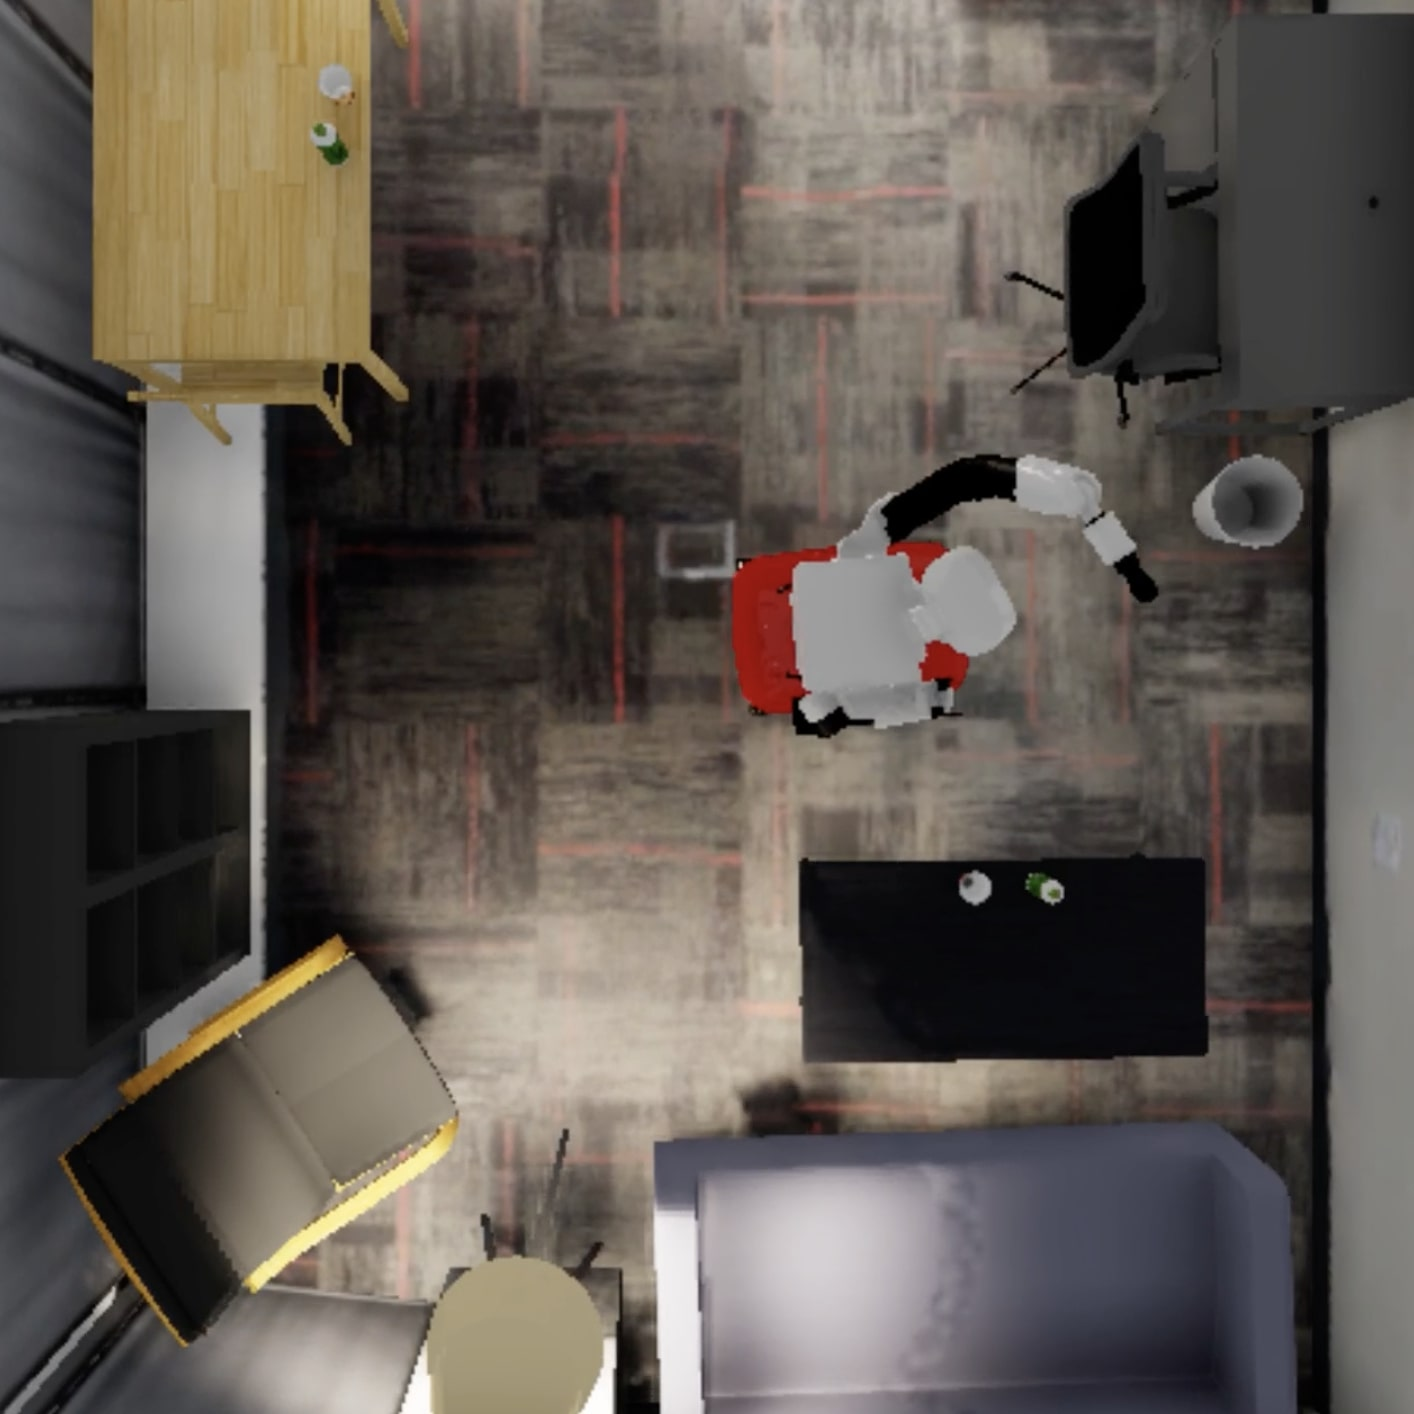
\includegraphics[trim=0 200 0 200,clip,width=0.33\linewidth]{figures/baseline_appendix/navigate_to_2}%
\hfill%
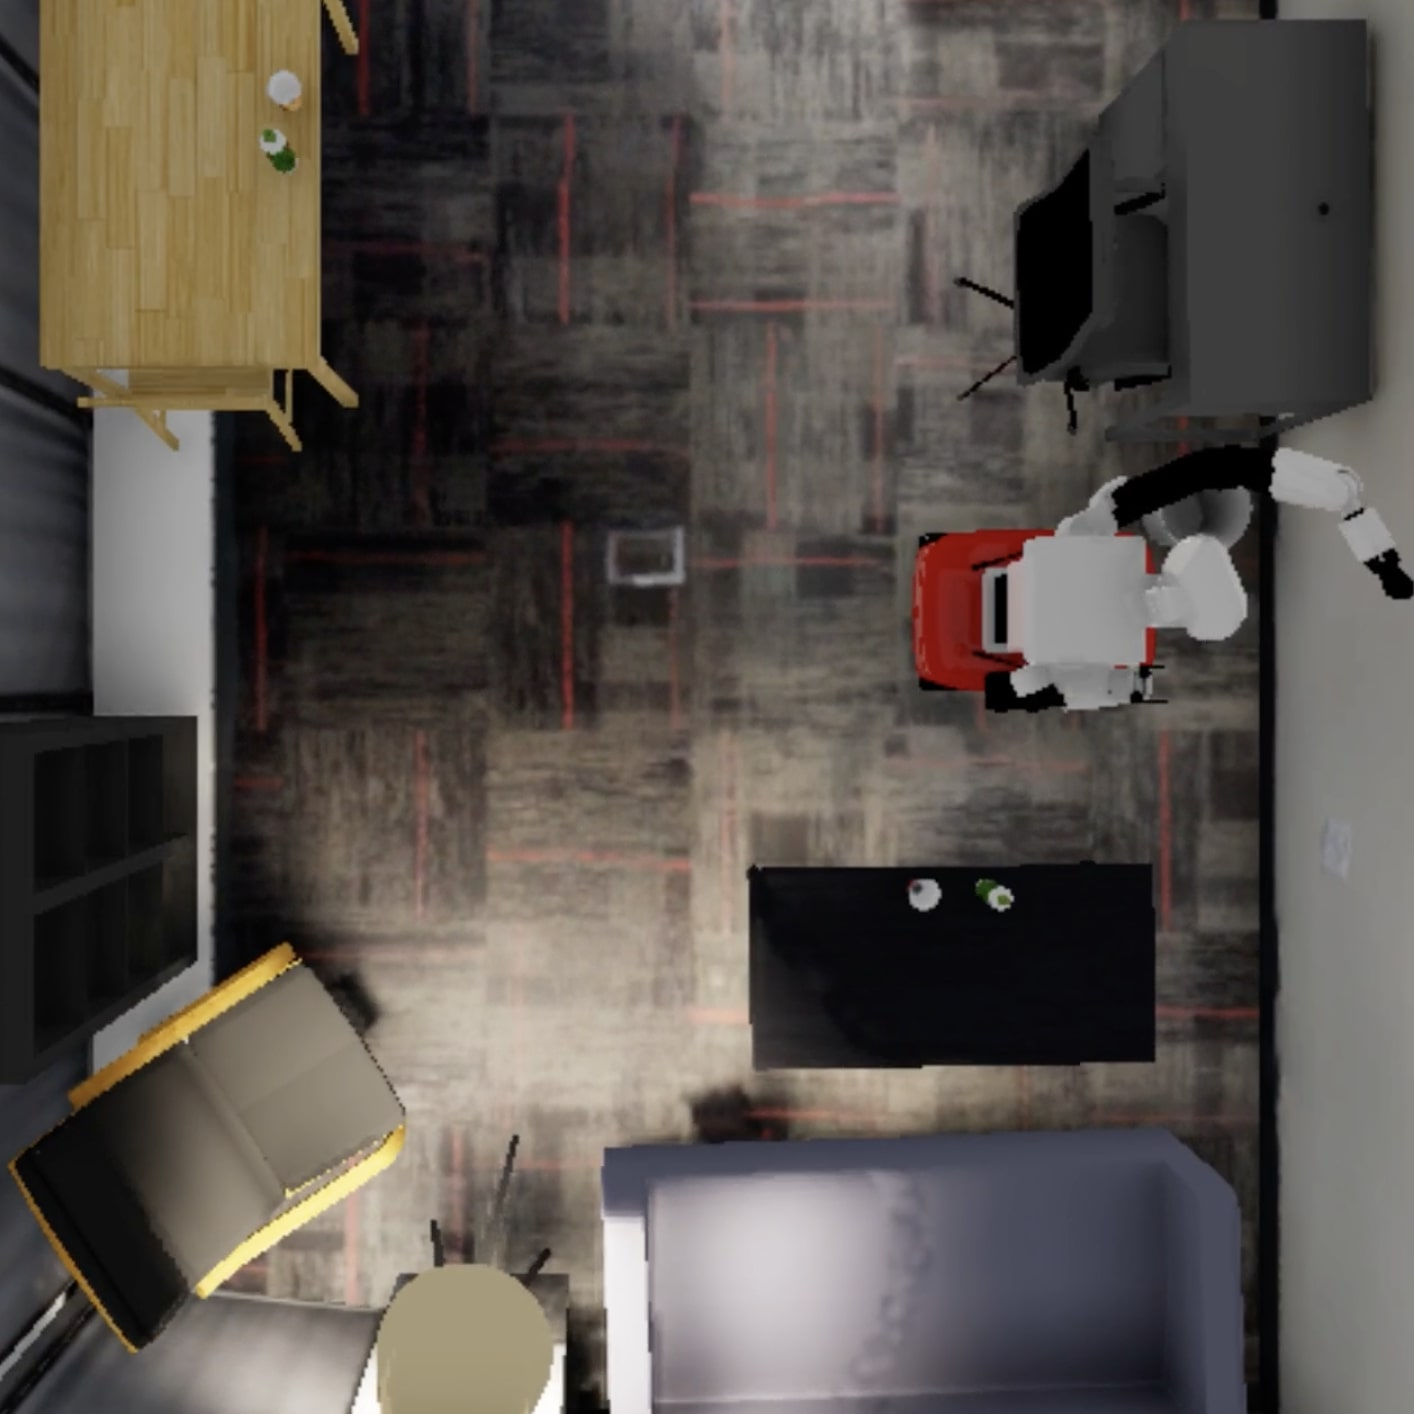
\includegraphics[trim=0 200 0 200,clip,width=0.33\linewidth]{figures/baseline_appendix/navigate_to_3}%
}
\vspace{-5pt}
\caption{\texttt{navigate}}
\vspace{10pt}
\end{subfigure}
\begin{subfigure}[t]{0.8\textwidth}{\centering
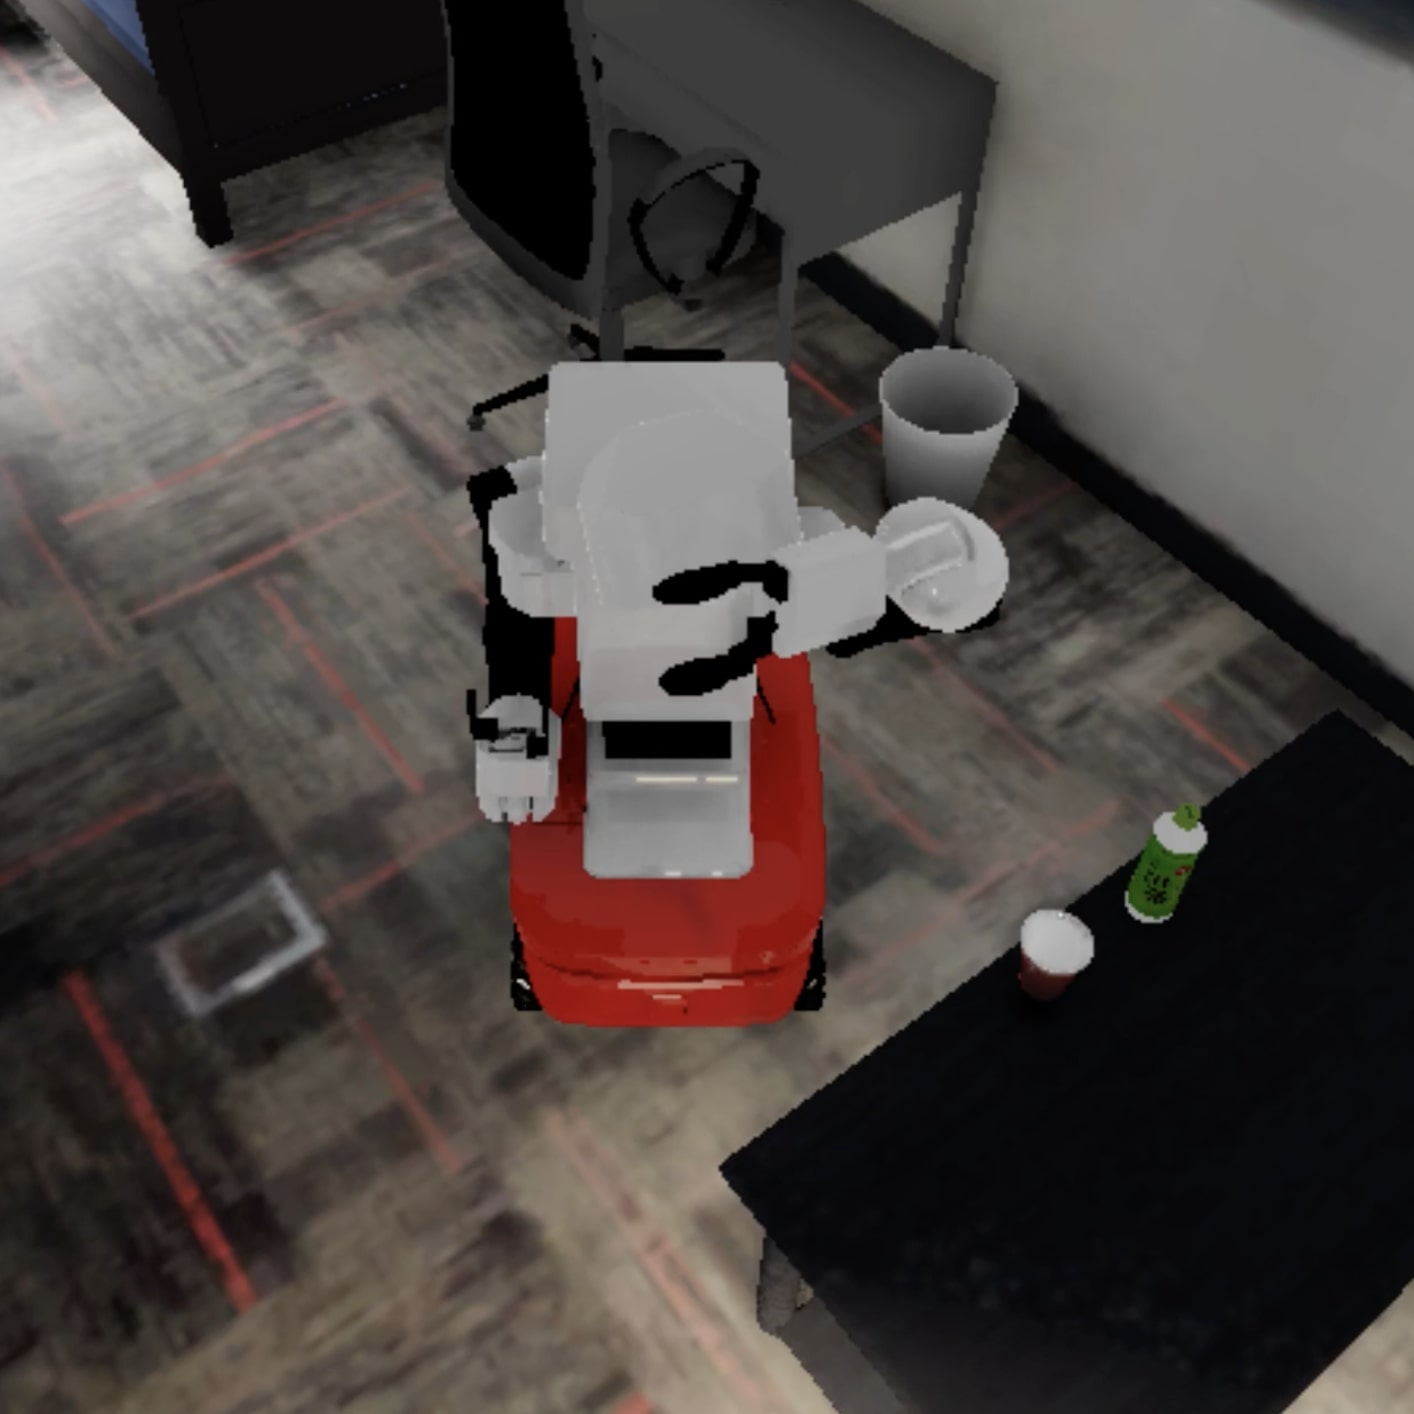
\includegraphics[trim=0 200 0 200,clip,width=0.33\linewidth]{figures/baseline_appendix/pick_1}%
\hfill%
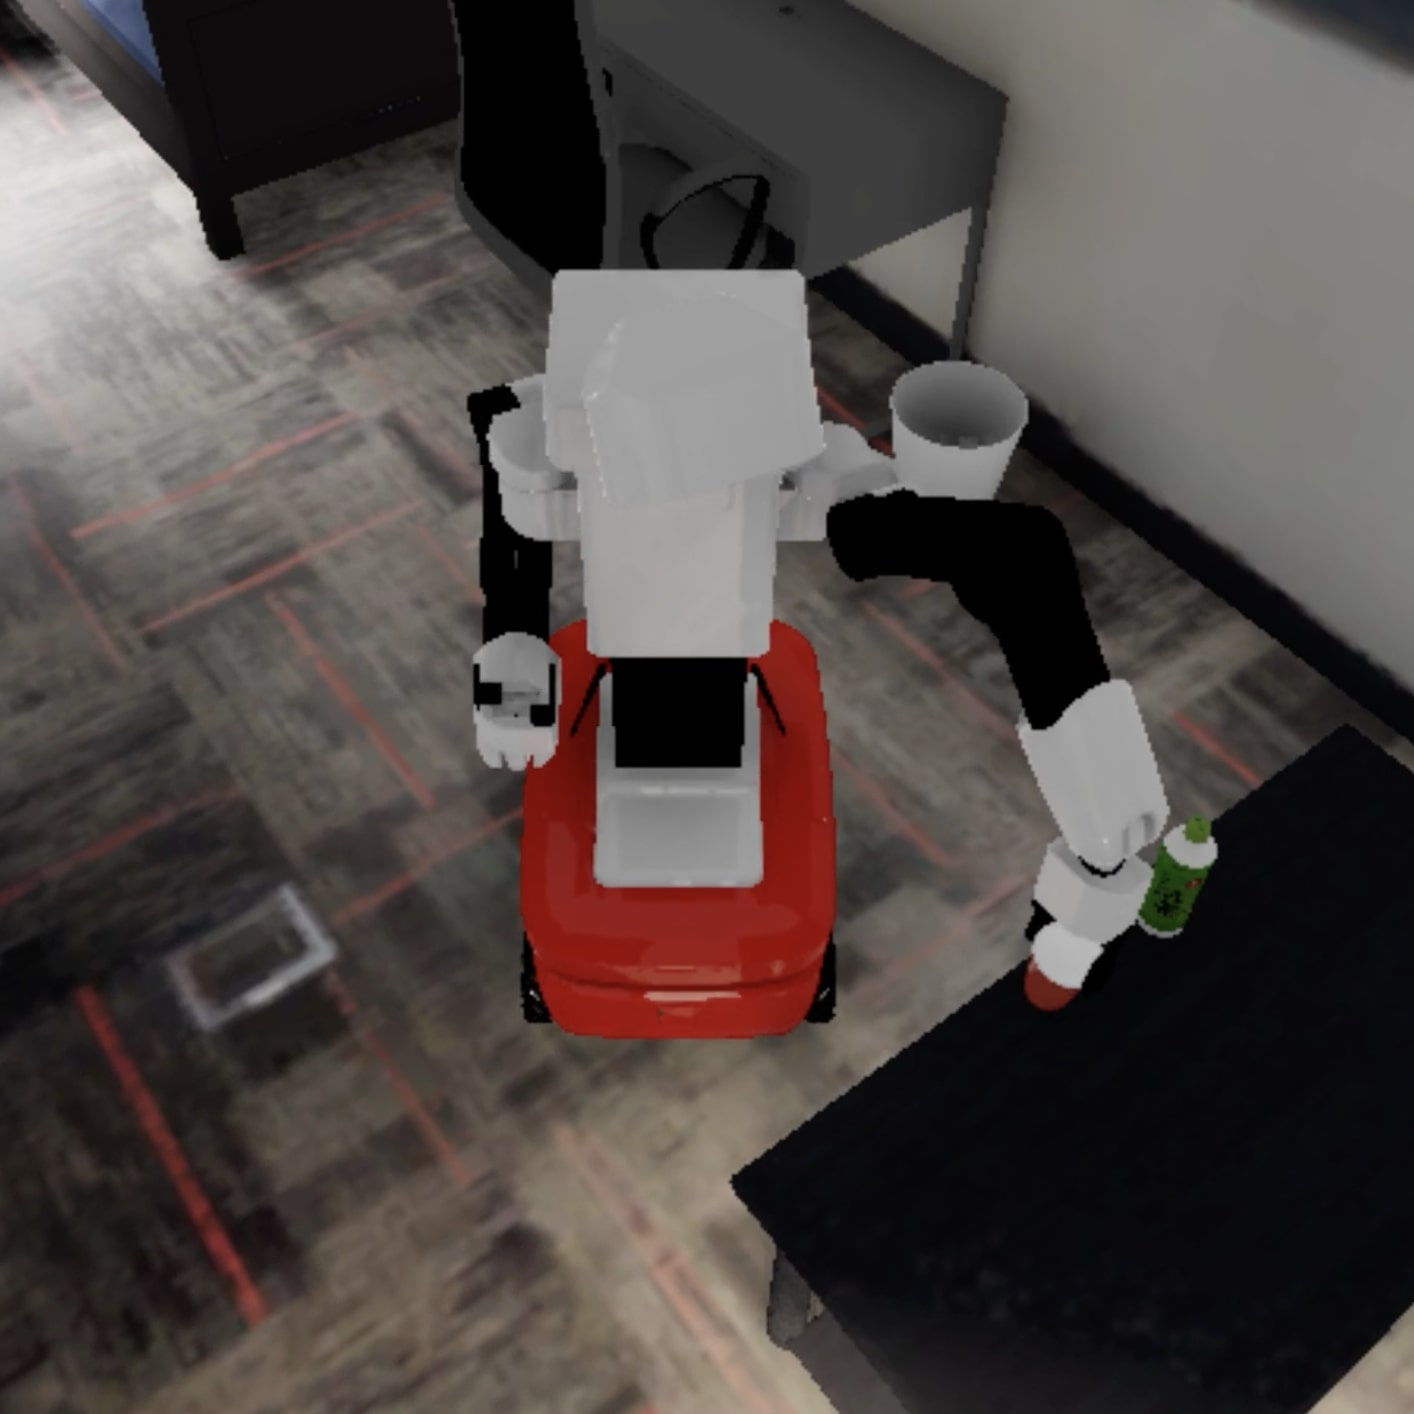
\includegraphics[trim=0 200 0 200,clip,width=0.33\linewidth]{figures/baseline_appendix/pick_2}%
\hfill%
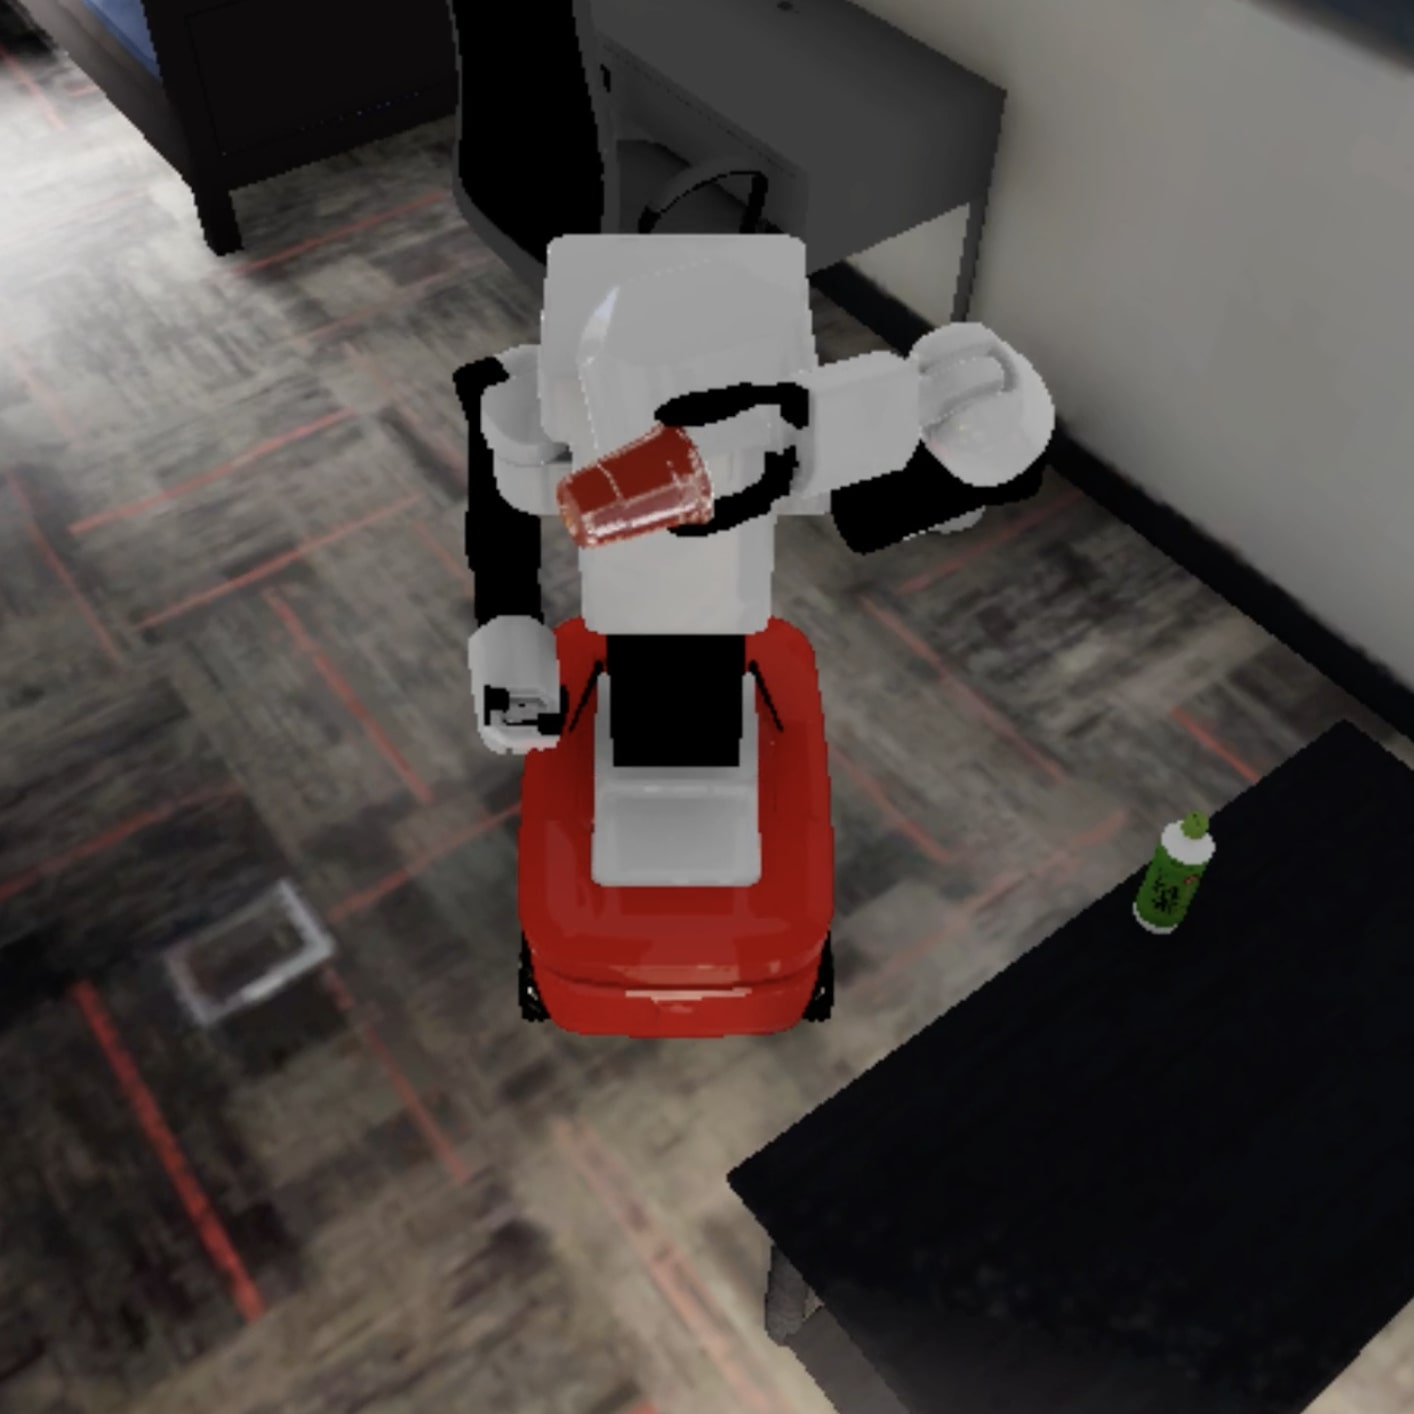
\includegraphics[trim=0 200 0 200,clip,width=0.33\linewidth]{figures/baseline_appendix/pick_3}
}%
\vspace{-5pt}%
\caption{\texttt{pick}}%
\vspace{10pt}%
\end{subfigure}
\begin{subfigure}[t]{0.8\textwidth}{\centering
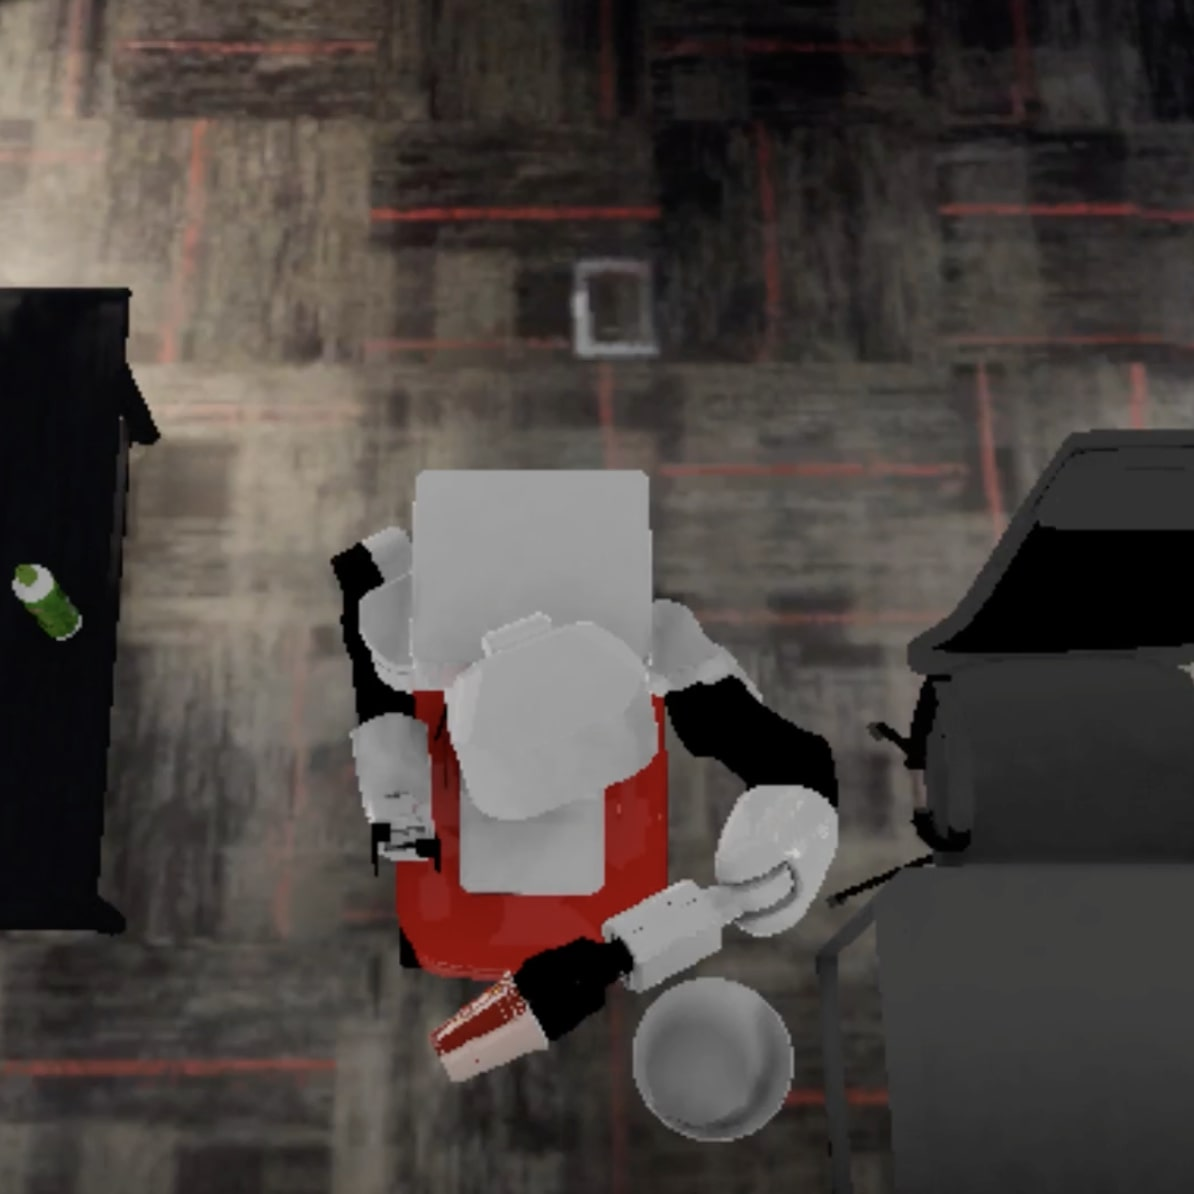
\includegraphics[trim=0 0 0 250,clip, width=0.33\linewidth]{figures/baseline_appendix/place_1}%
\hfill%
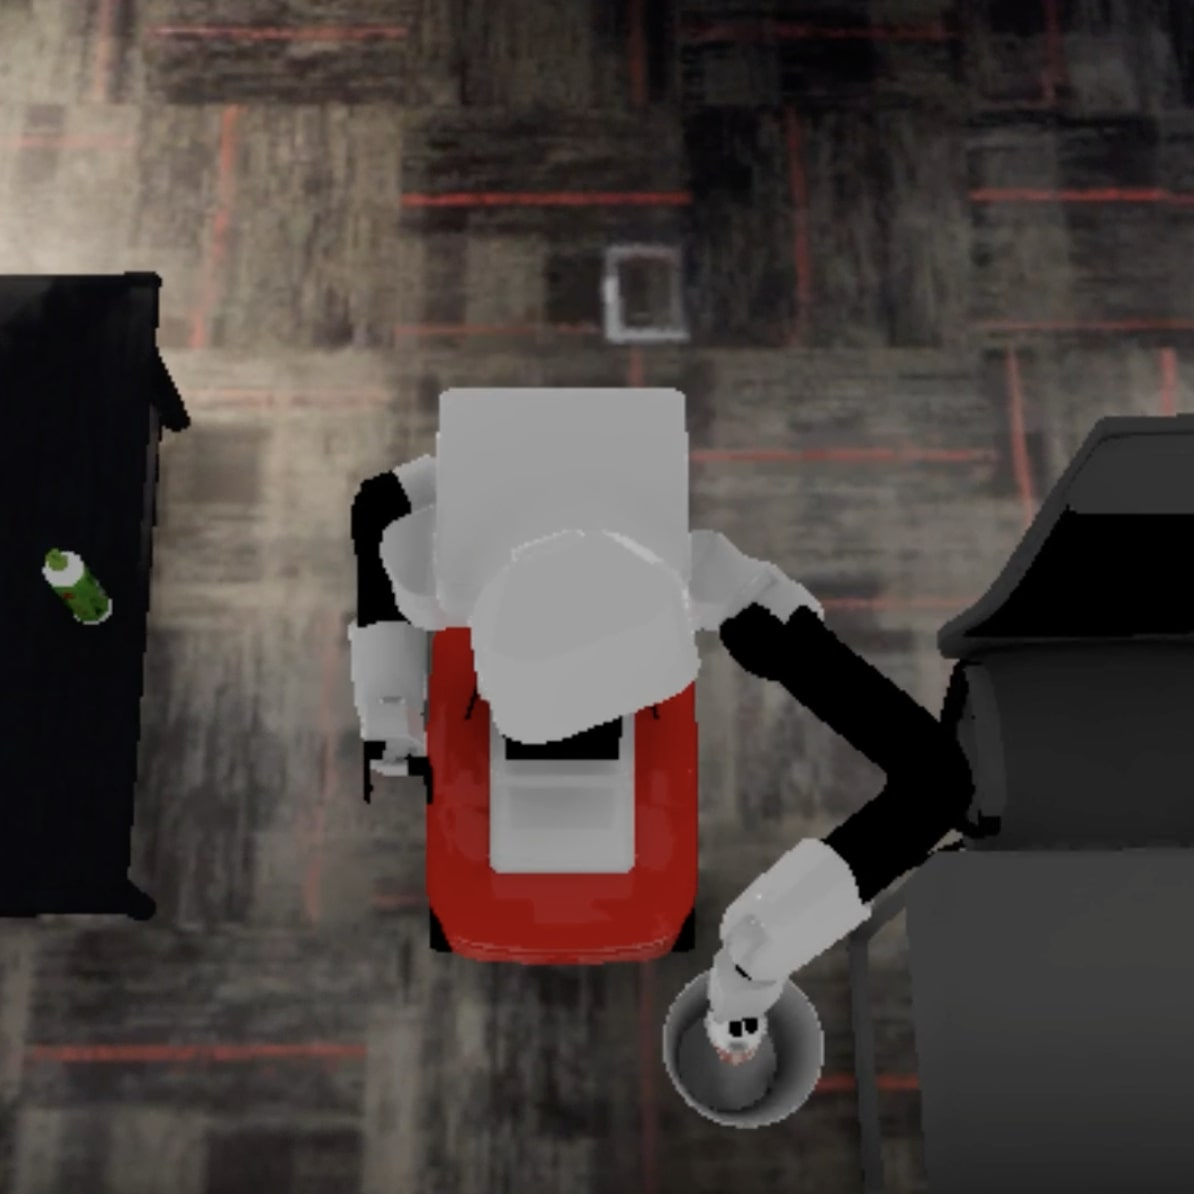
\includegraphics[trim=0 0 0 250,clip,width=0.33\linewidth]{figures/baseline_appendix/place_2}%
\hfill%
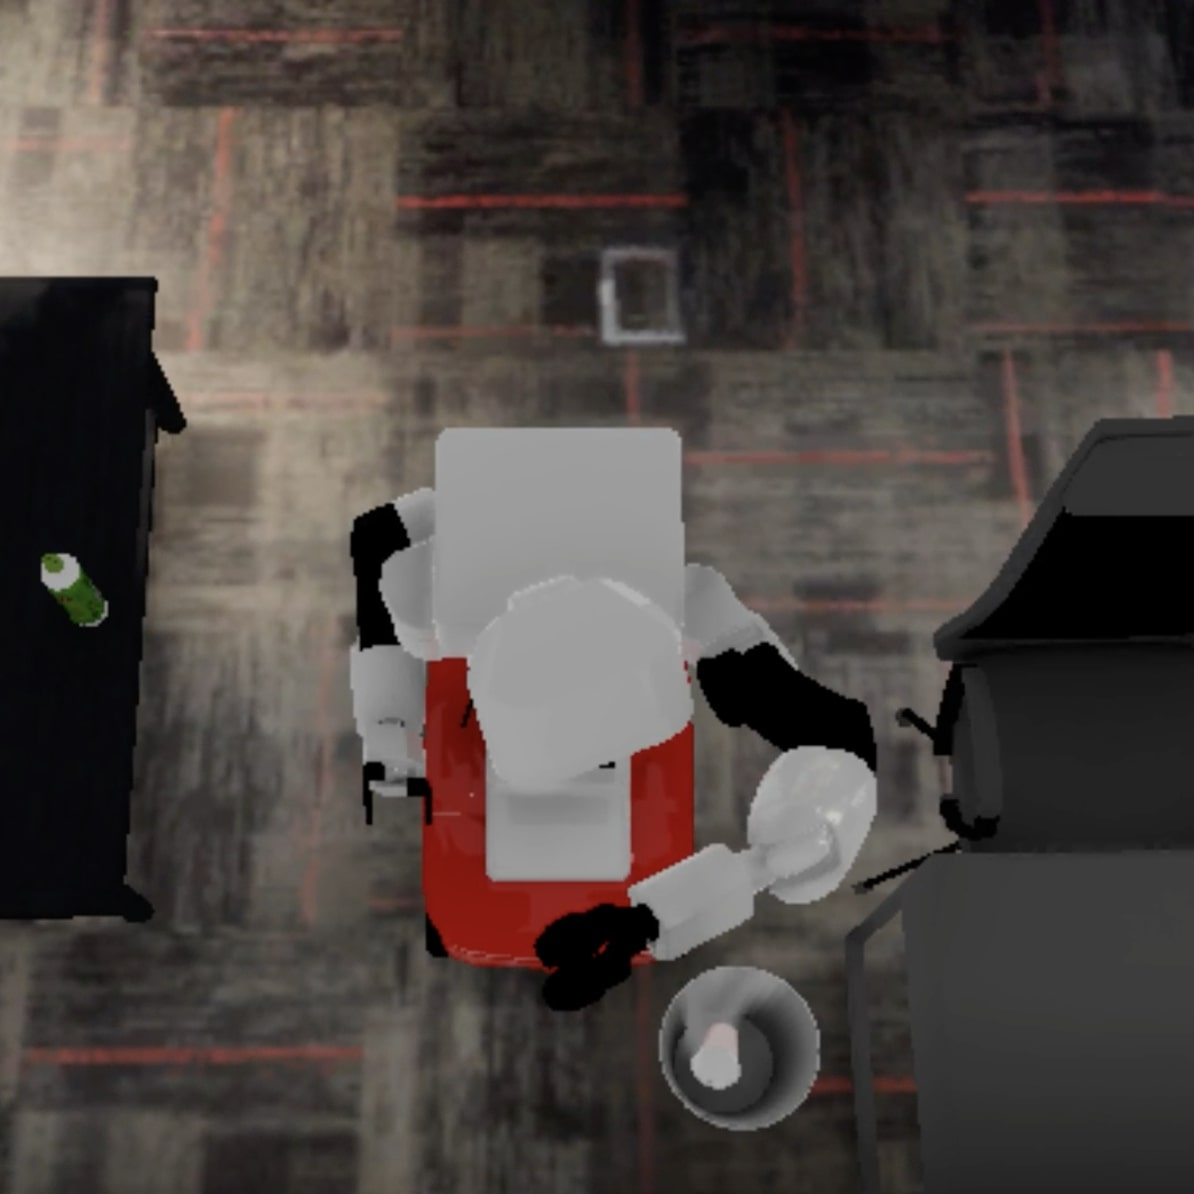
\includegraphics[trim=0 0 0 250,clip,width=0.33\linewidth]{figures/baseline_appendix/place_3}
}%
\vspace{-5pt}%
\caption{\texttt{place}}%
\vspace{10pt}%
\end{subfigure}
\begin{subfigure}[t]{0.8\textwidth}{\centering
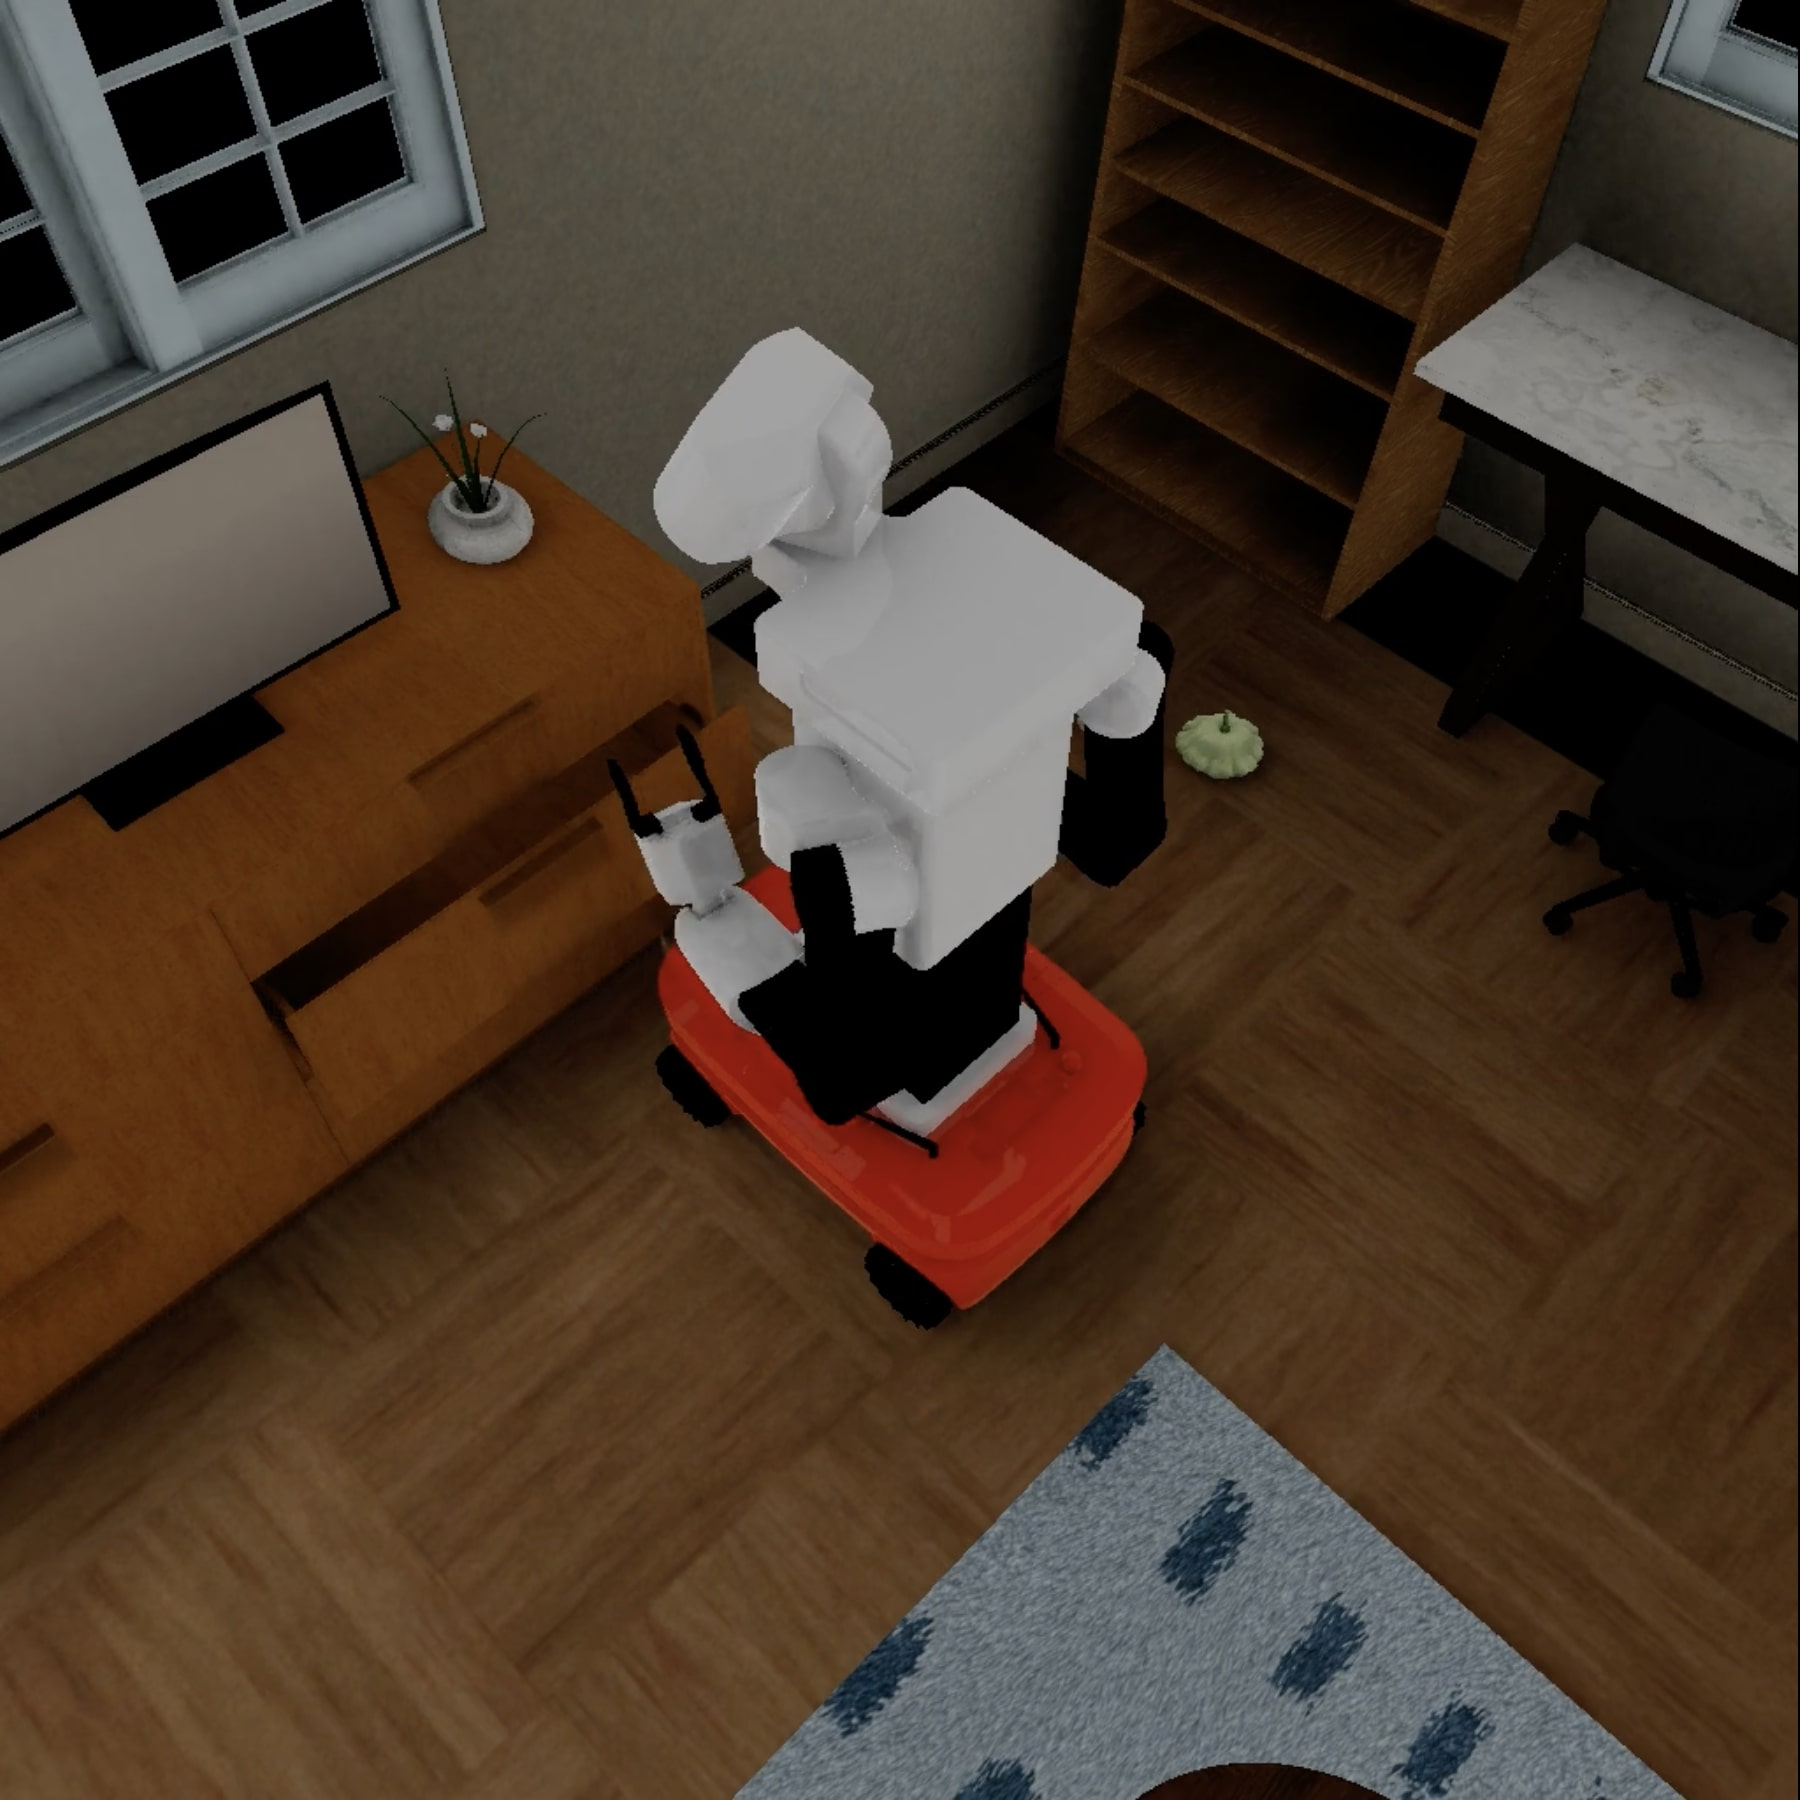
\includegraphics[trim=0 220 0 20,clip,width=0.33\linewidth]{figures/baseline_appendix/pull_1}%
\hfill%
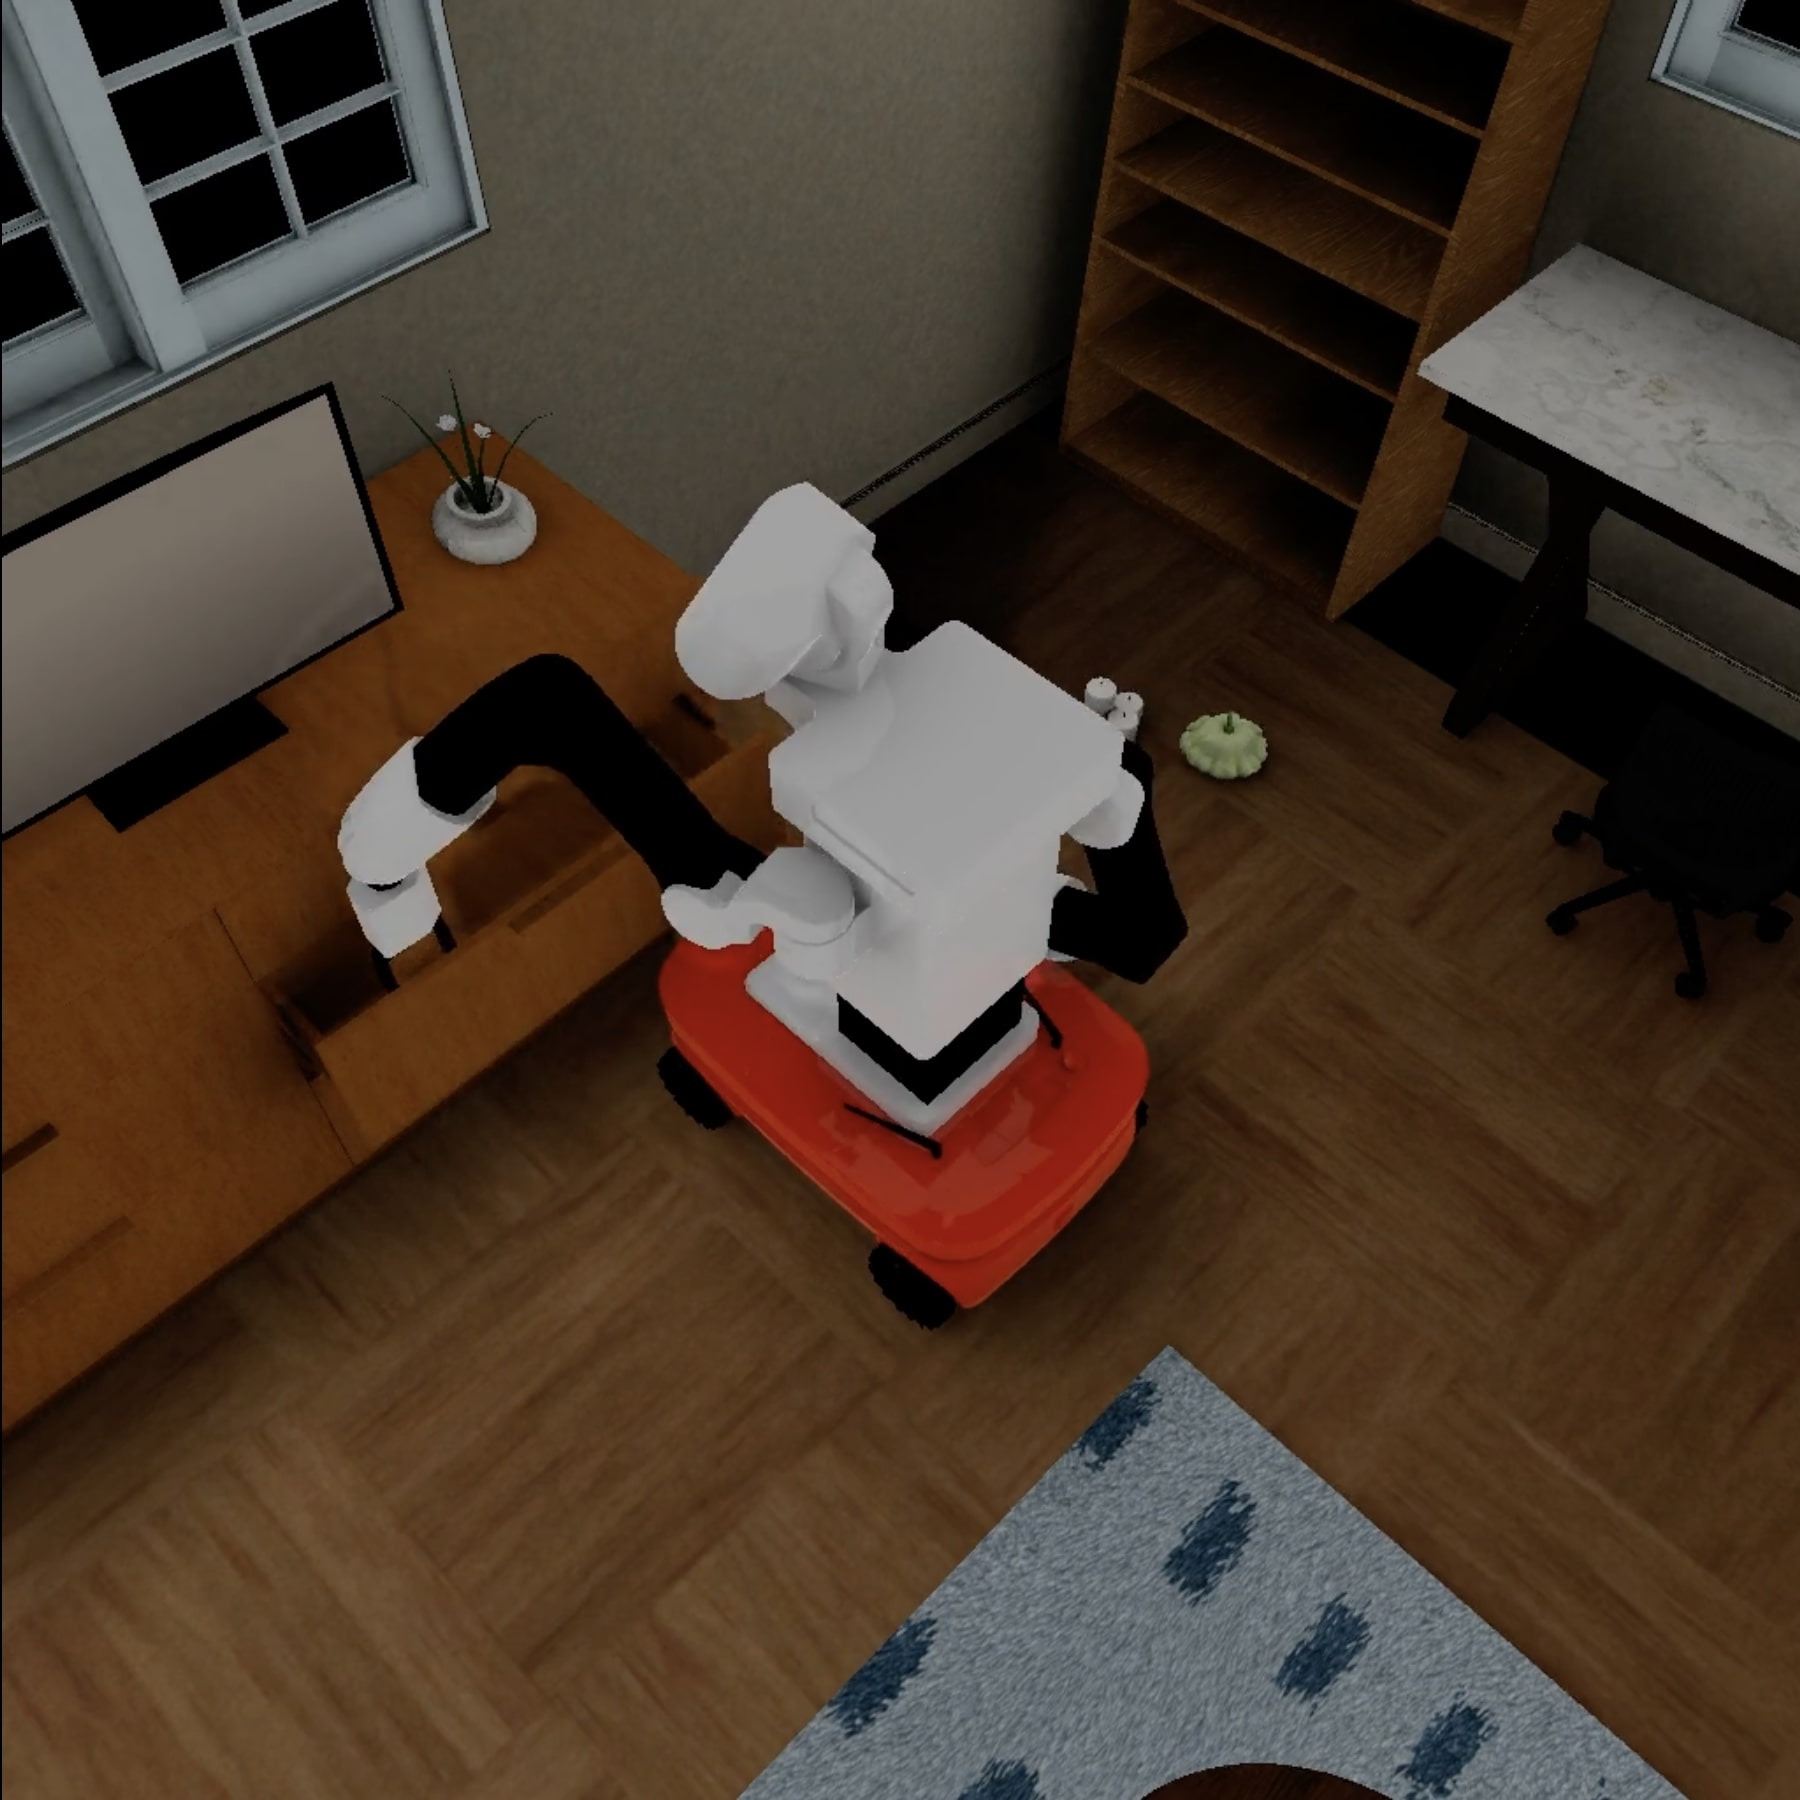
\includegraphics[trim=0 220 0 20,clip,width=0.33\linewidth]{figures/baseline_appendix/pull_2}%
\hfill%
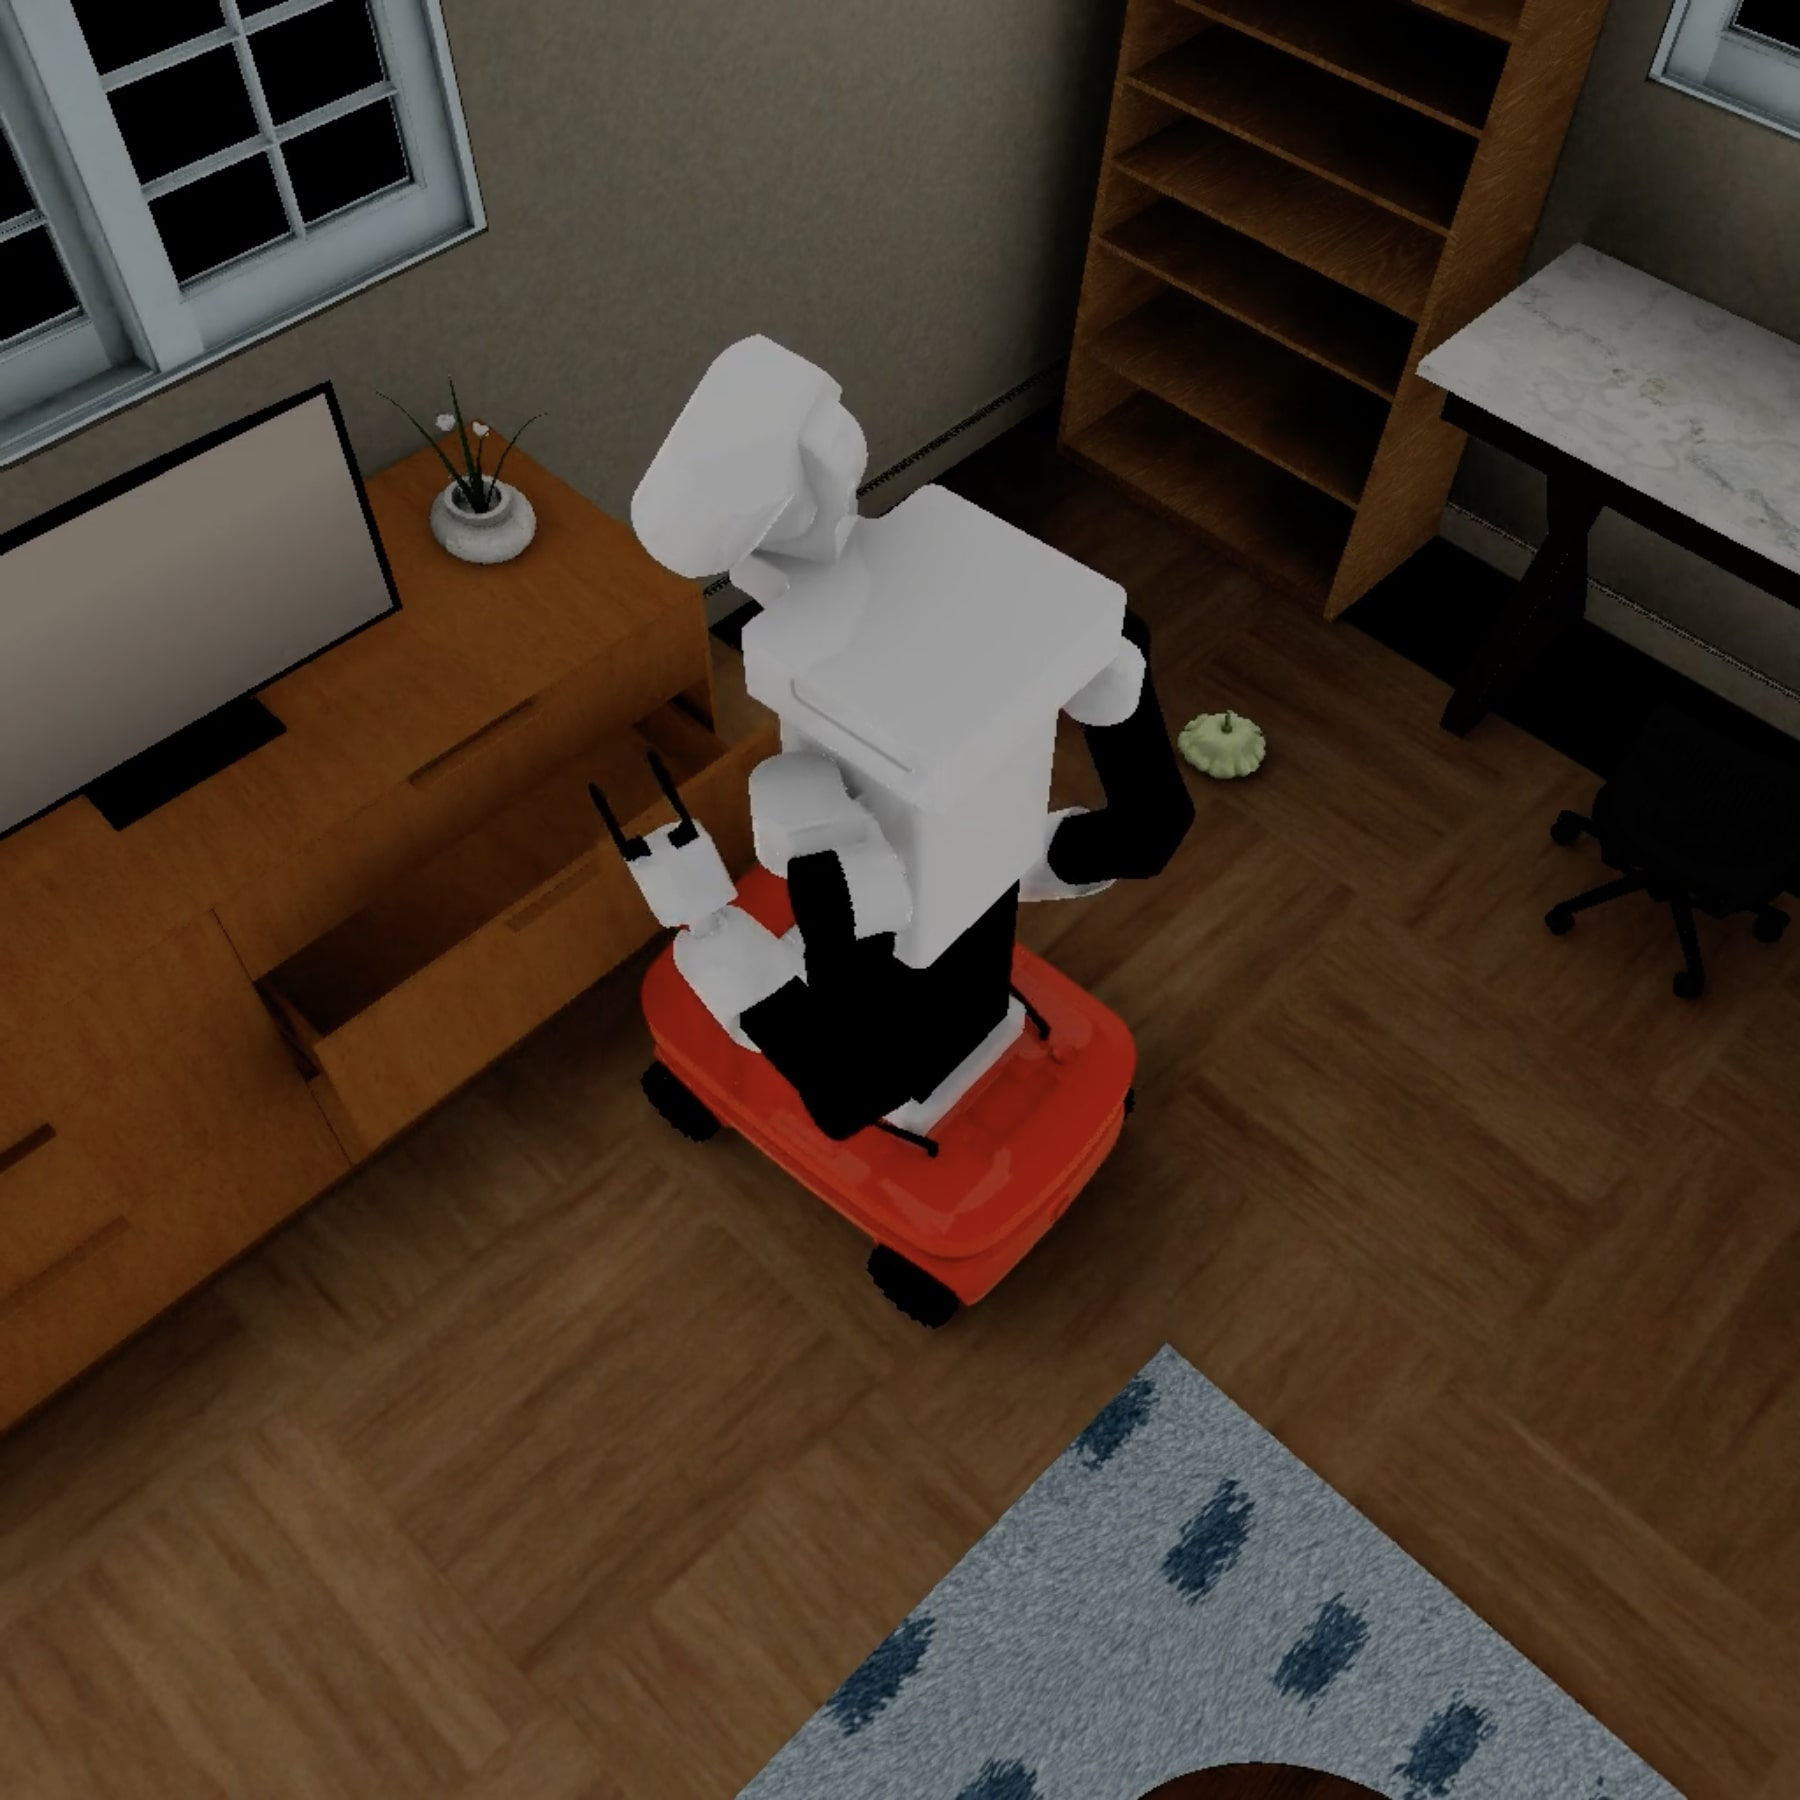
\includegraphics[trim=0 220 0 20,clip,width=0.33\linewidth]{figures/baseline_appendix/pull_3}
}%
\vspace{-5pt}
\caption{\texttt{push} (open)}
\vspace{10pt}
\end{subfigure}
\begin{subfigure}[t]{0.8\textwidth}{\centering
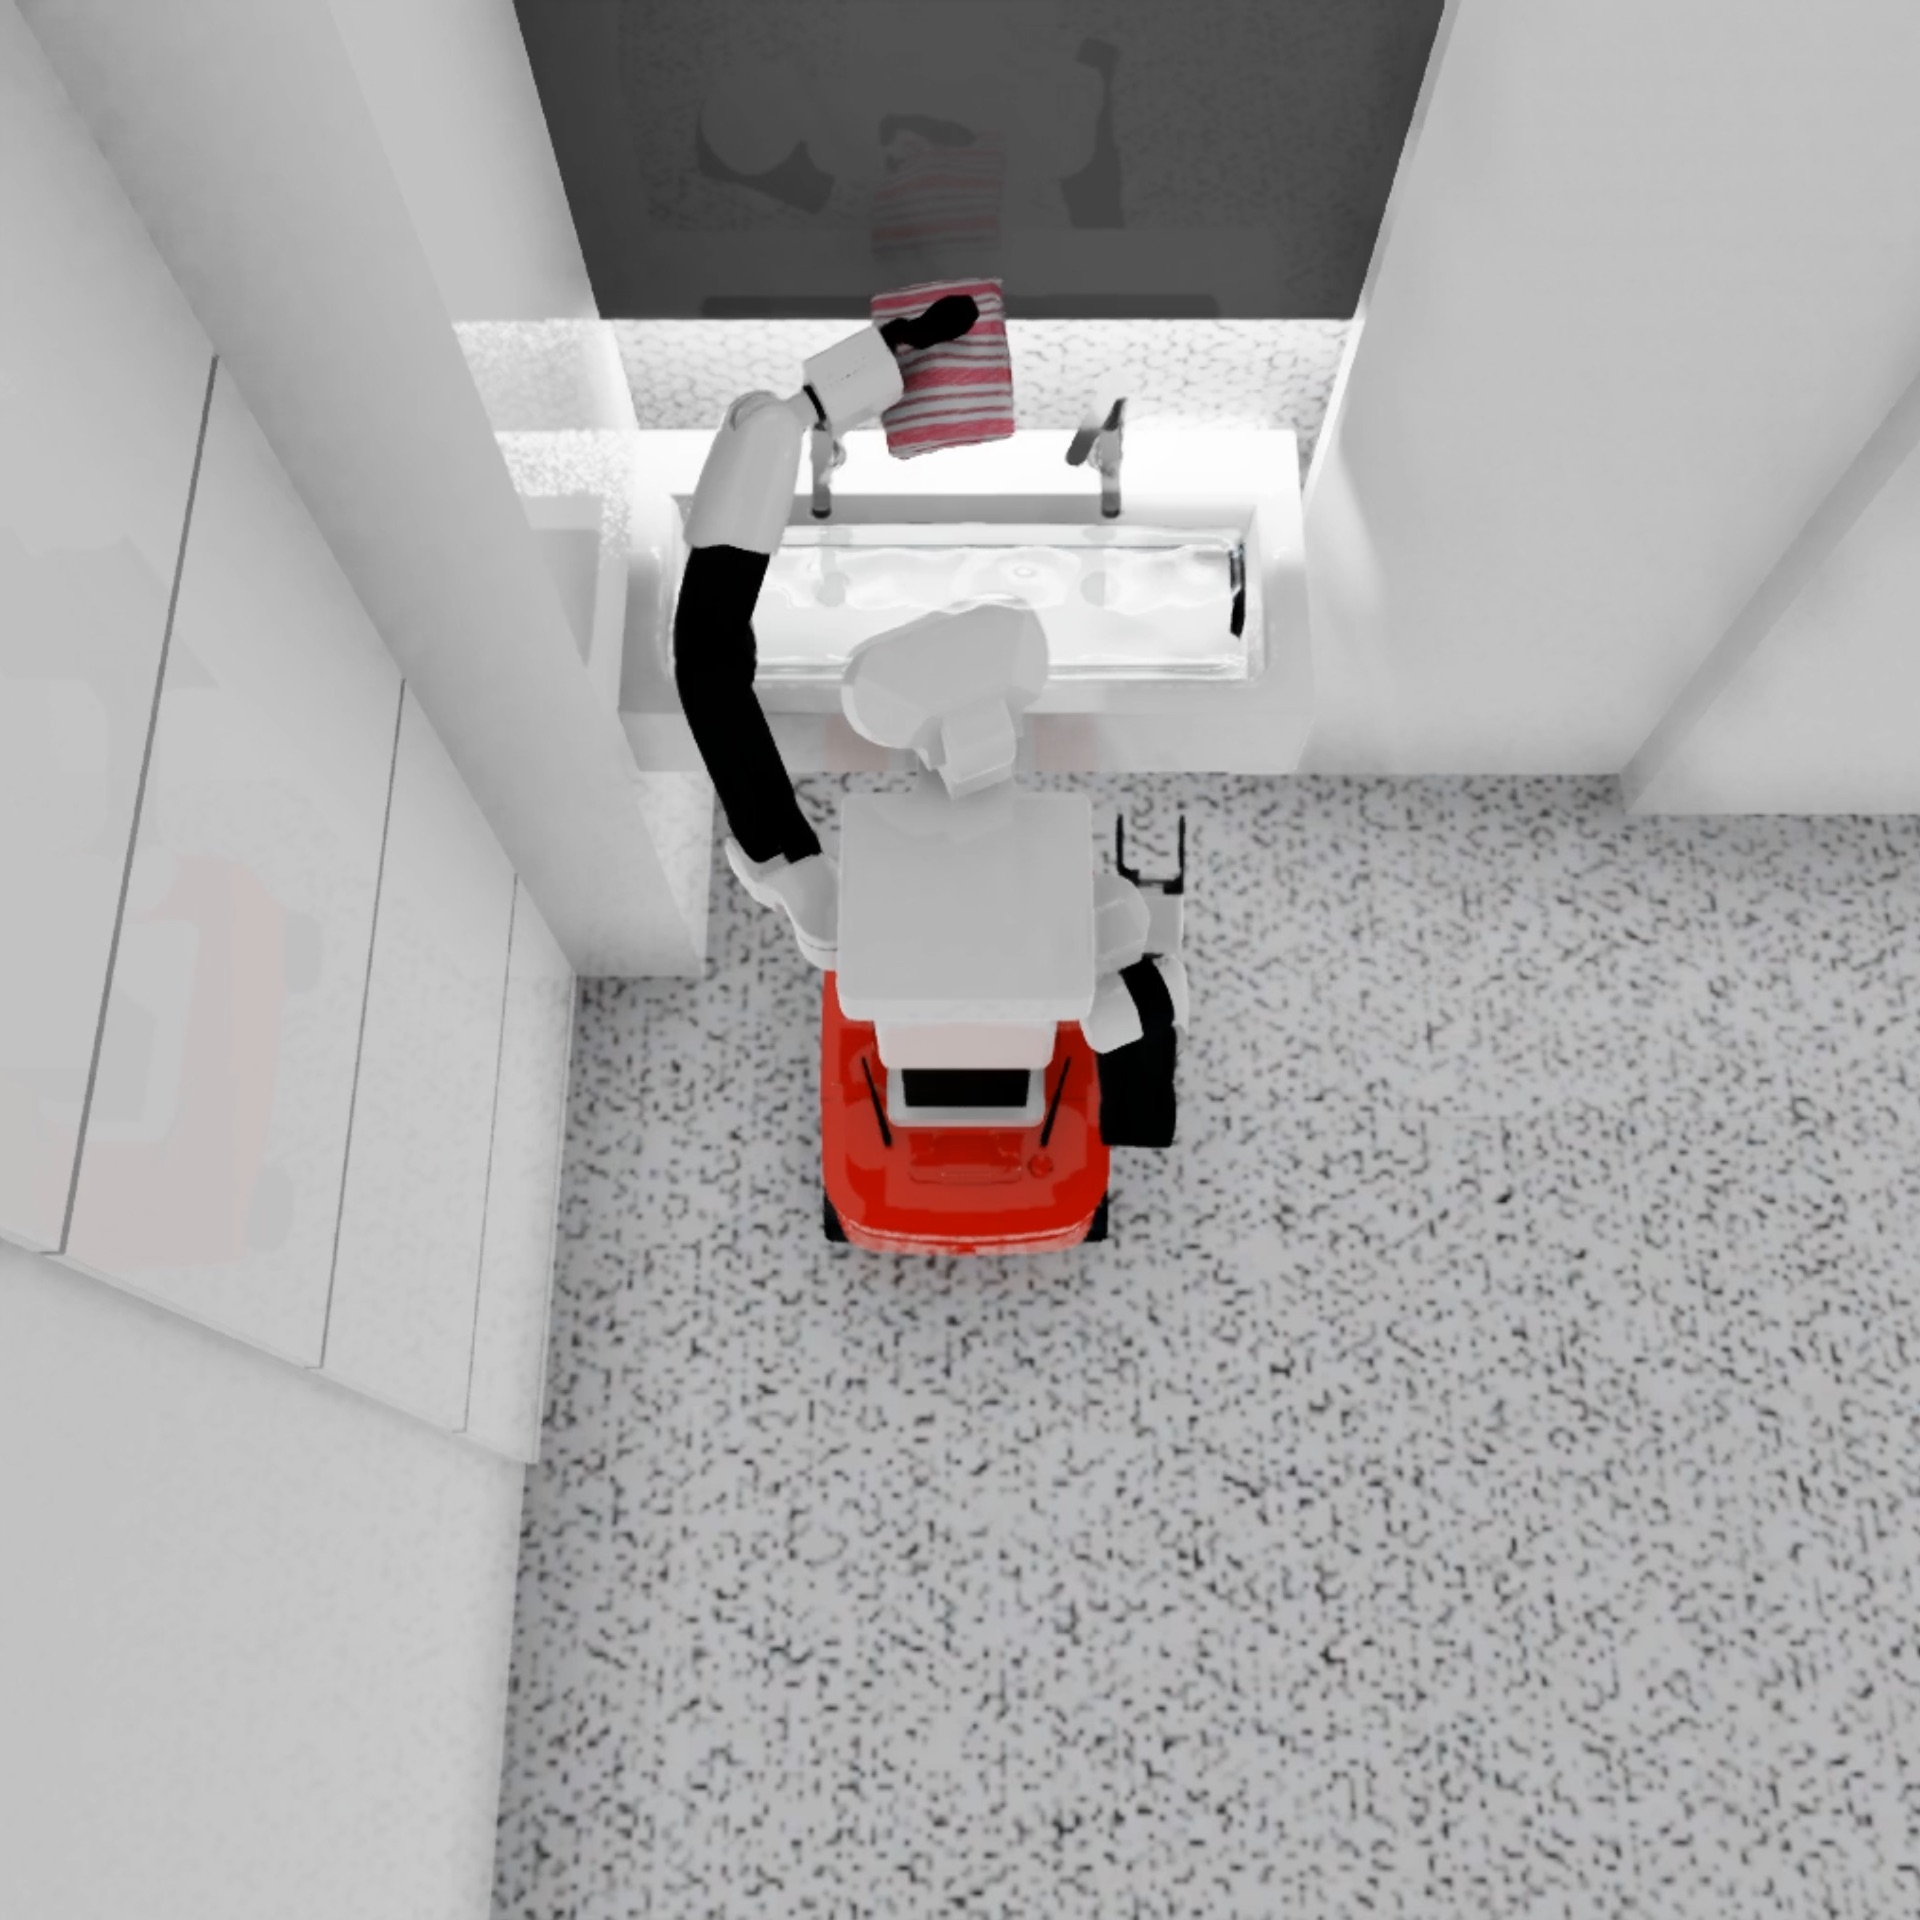
\includegraphics[trim=0 200 0 200,clip,width=0.33\linewidth]{figures/baseline_appendix/dip_1}%
\hfill%
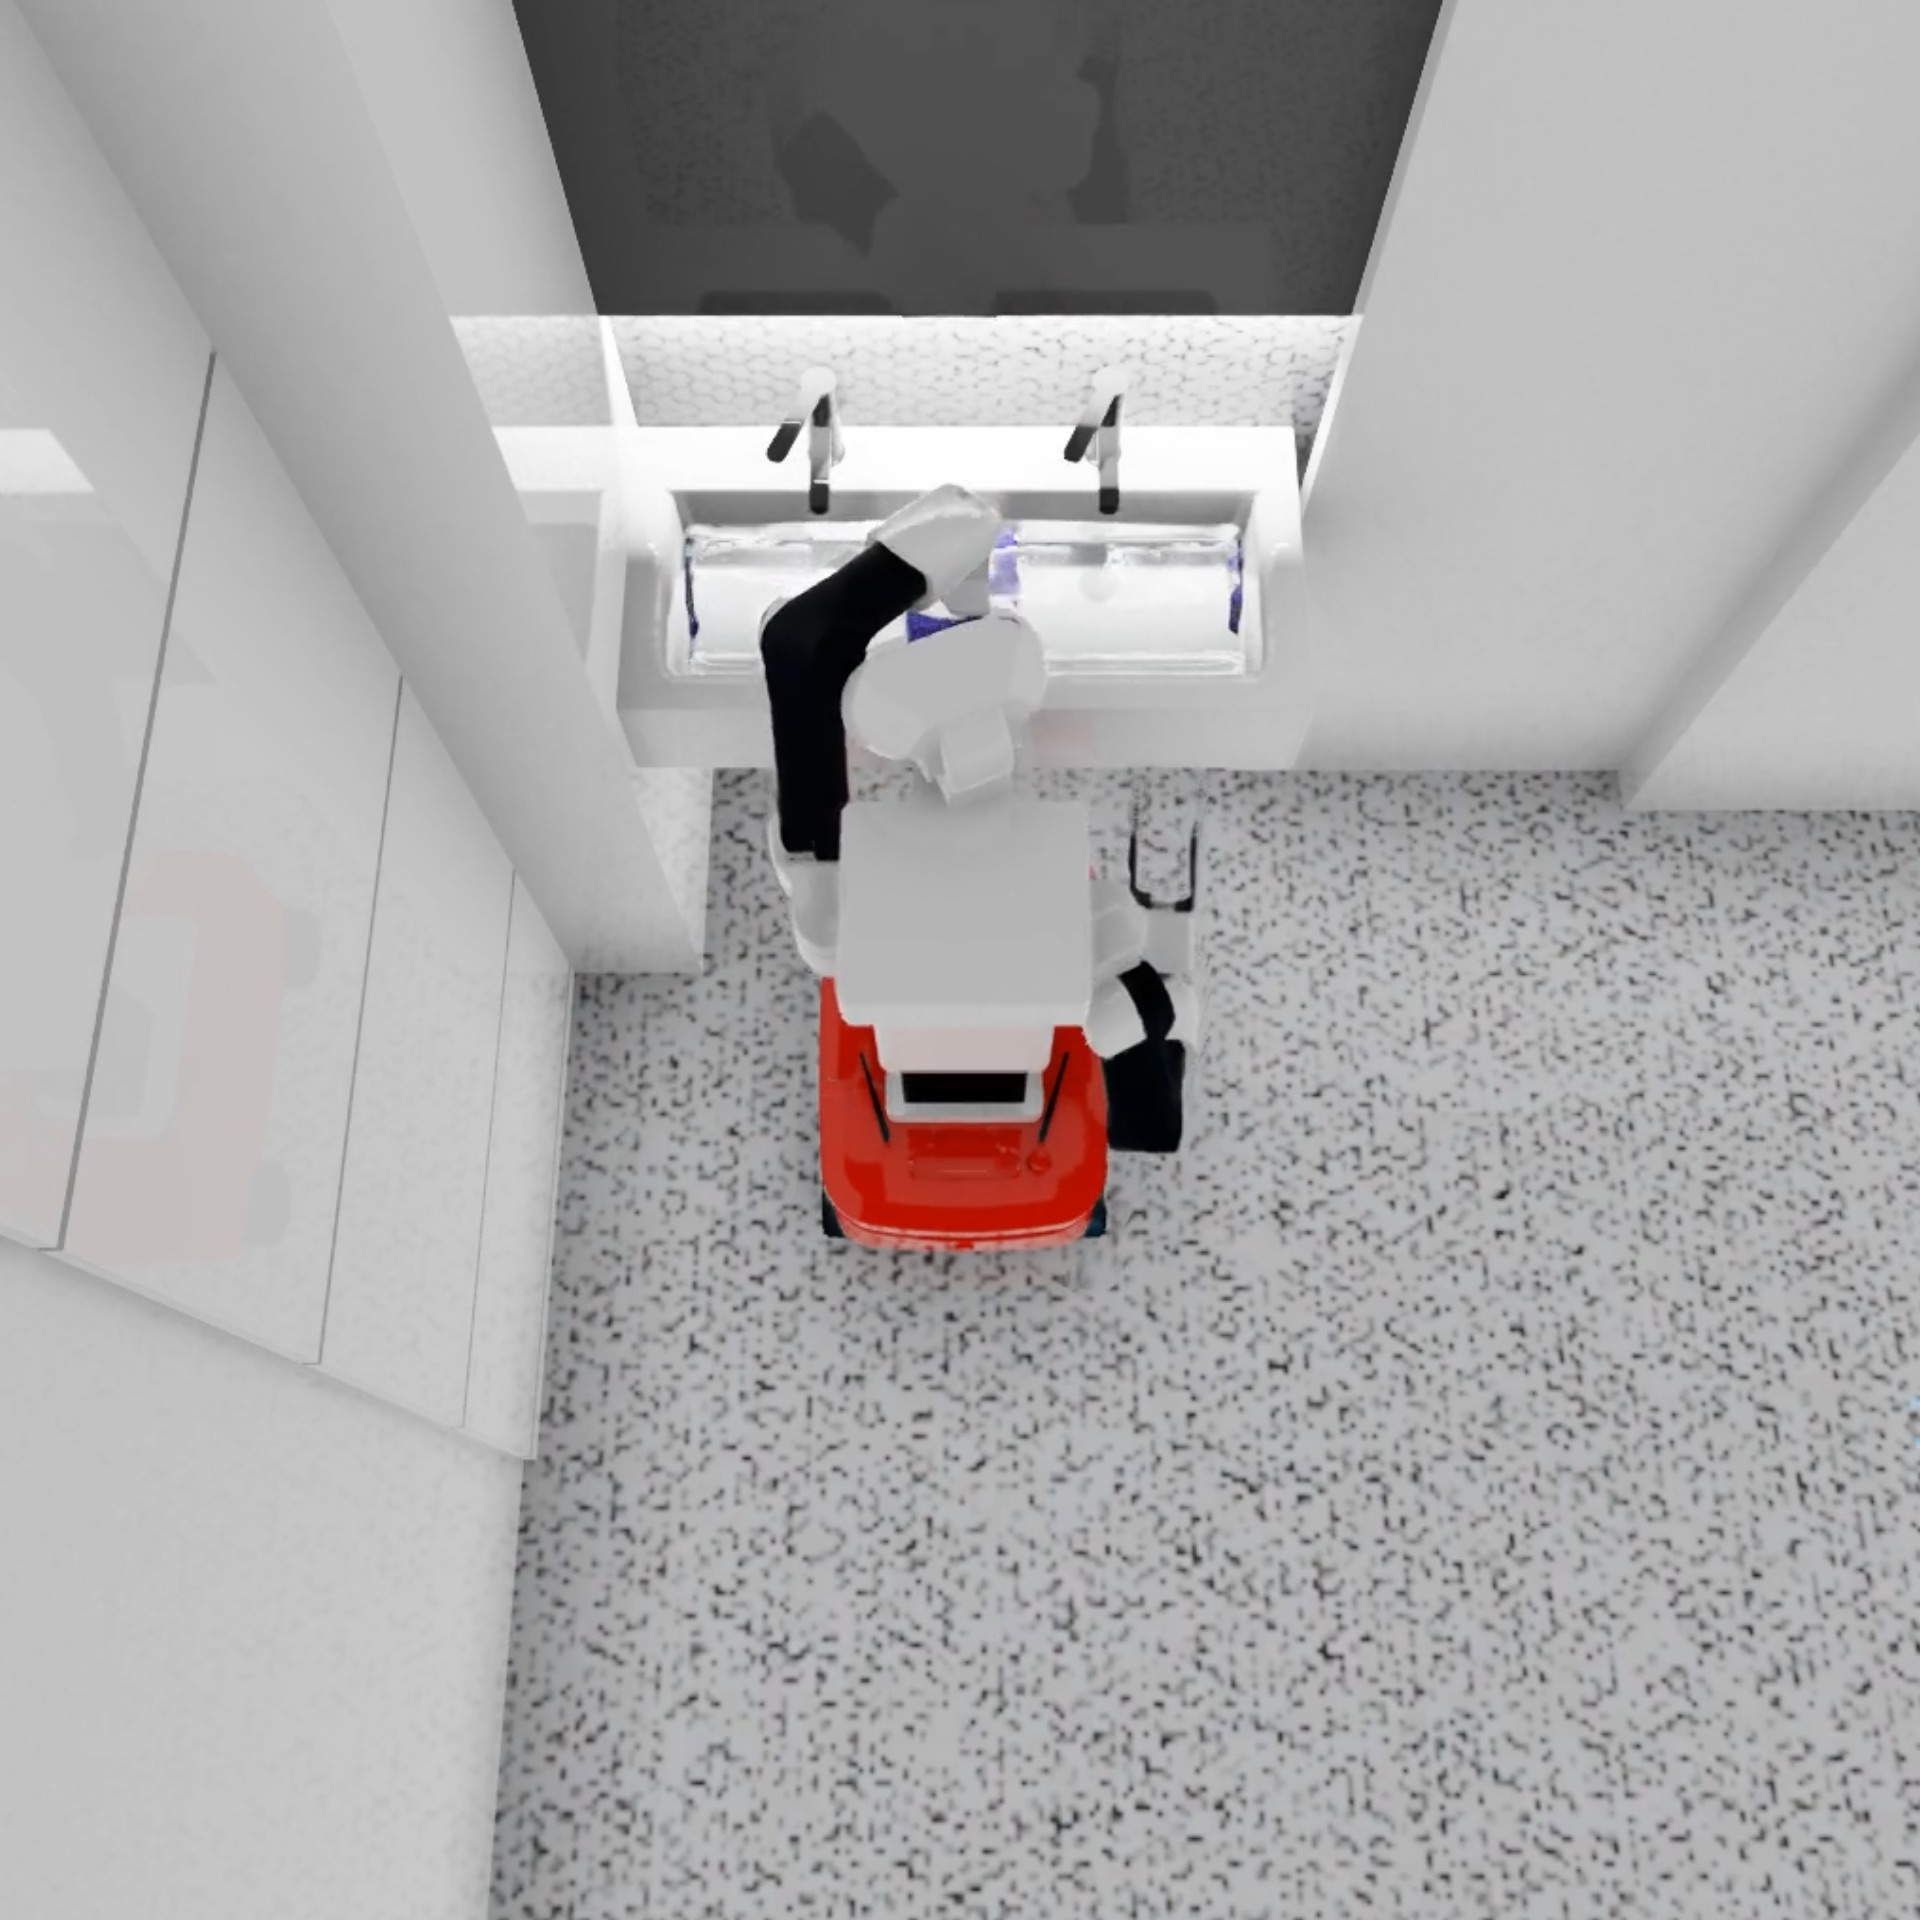
\includegraphics[trim=0 200 0 200,clip,width=0.33\linewidth]{figures/baseline_appendix/dip_2}%
\hfill%
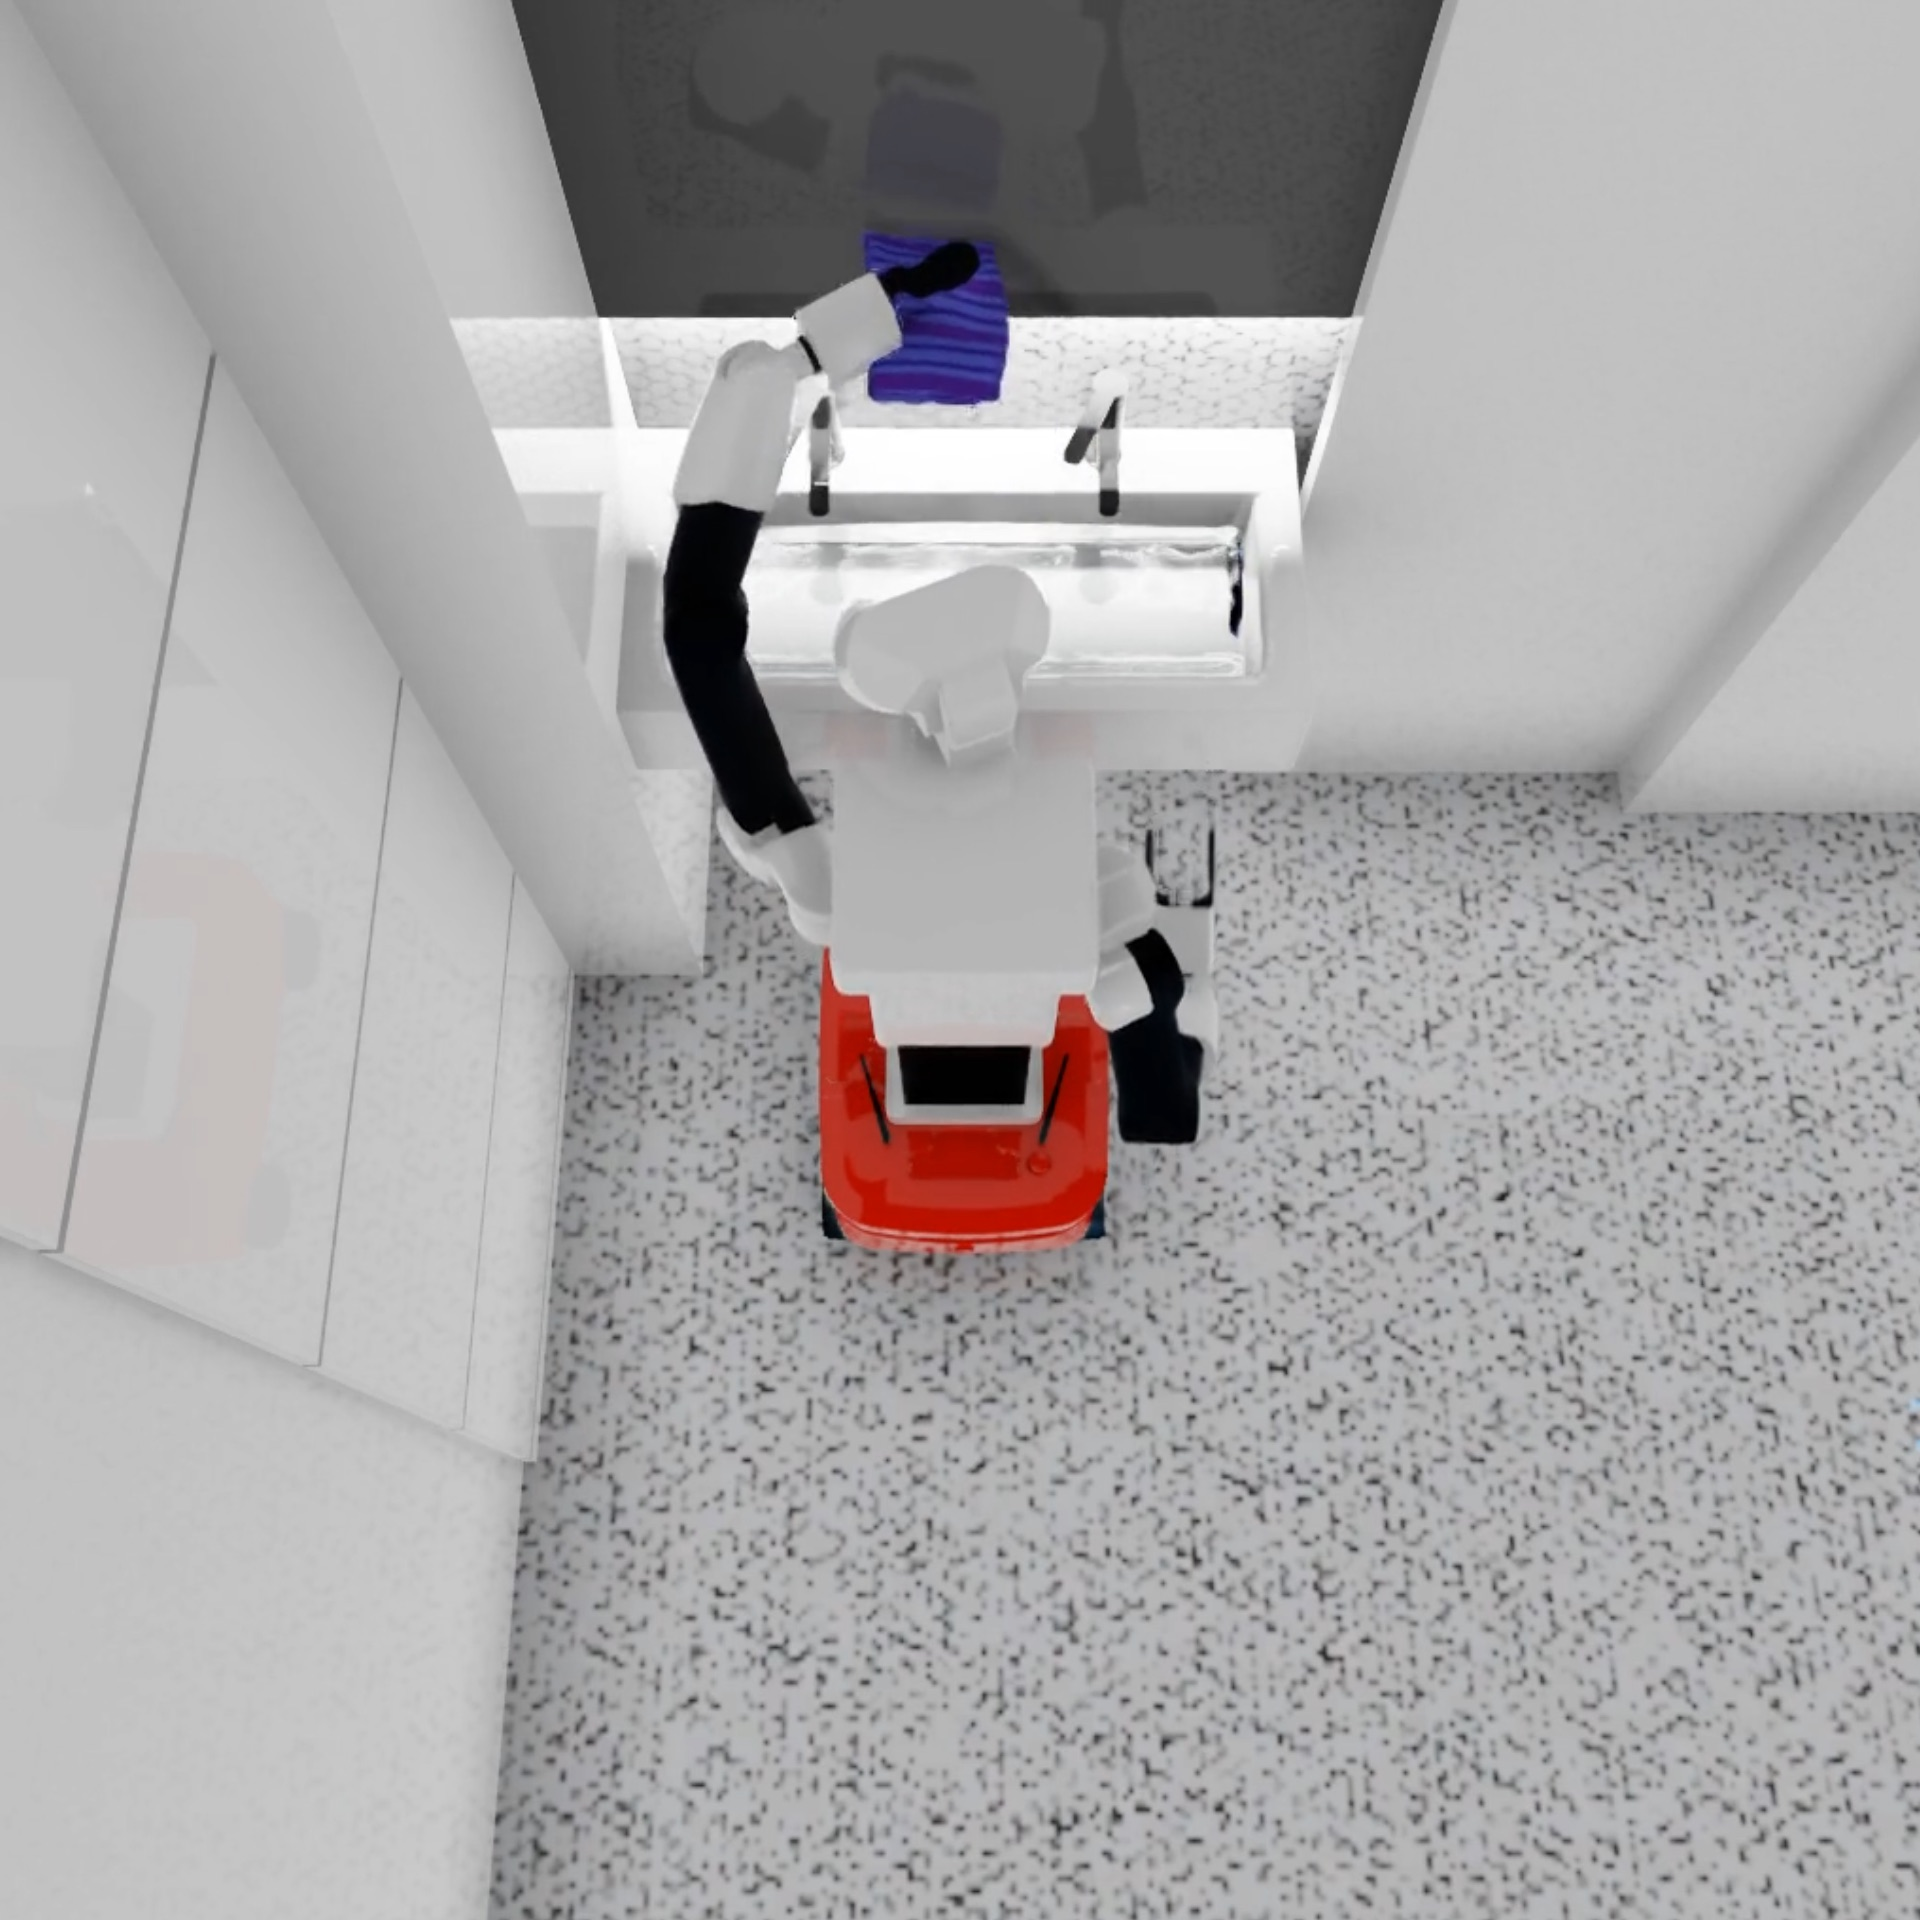
\includegraphics[trim=0 200 0 200,clip,width=0.33\linewidth]{figures/baseline_appendix/dip_3}
}%
\vspace{-5pt}%
\caption{\texttt{dip}}%
\vspace{10pt}%
\end{subfigure}
\begin{subfigure}[t]{0.8\textwidth}{\centering%
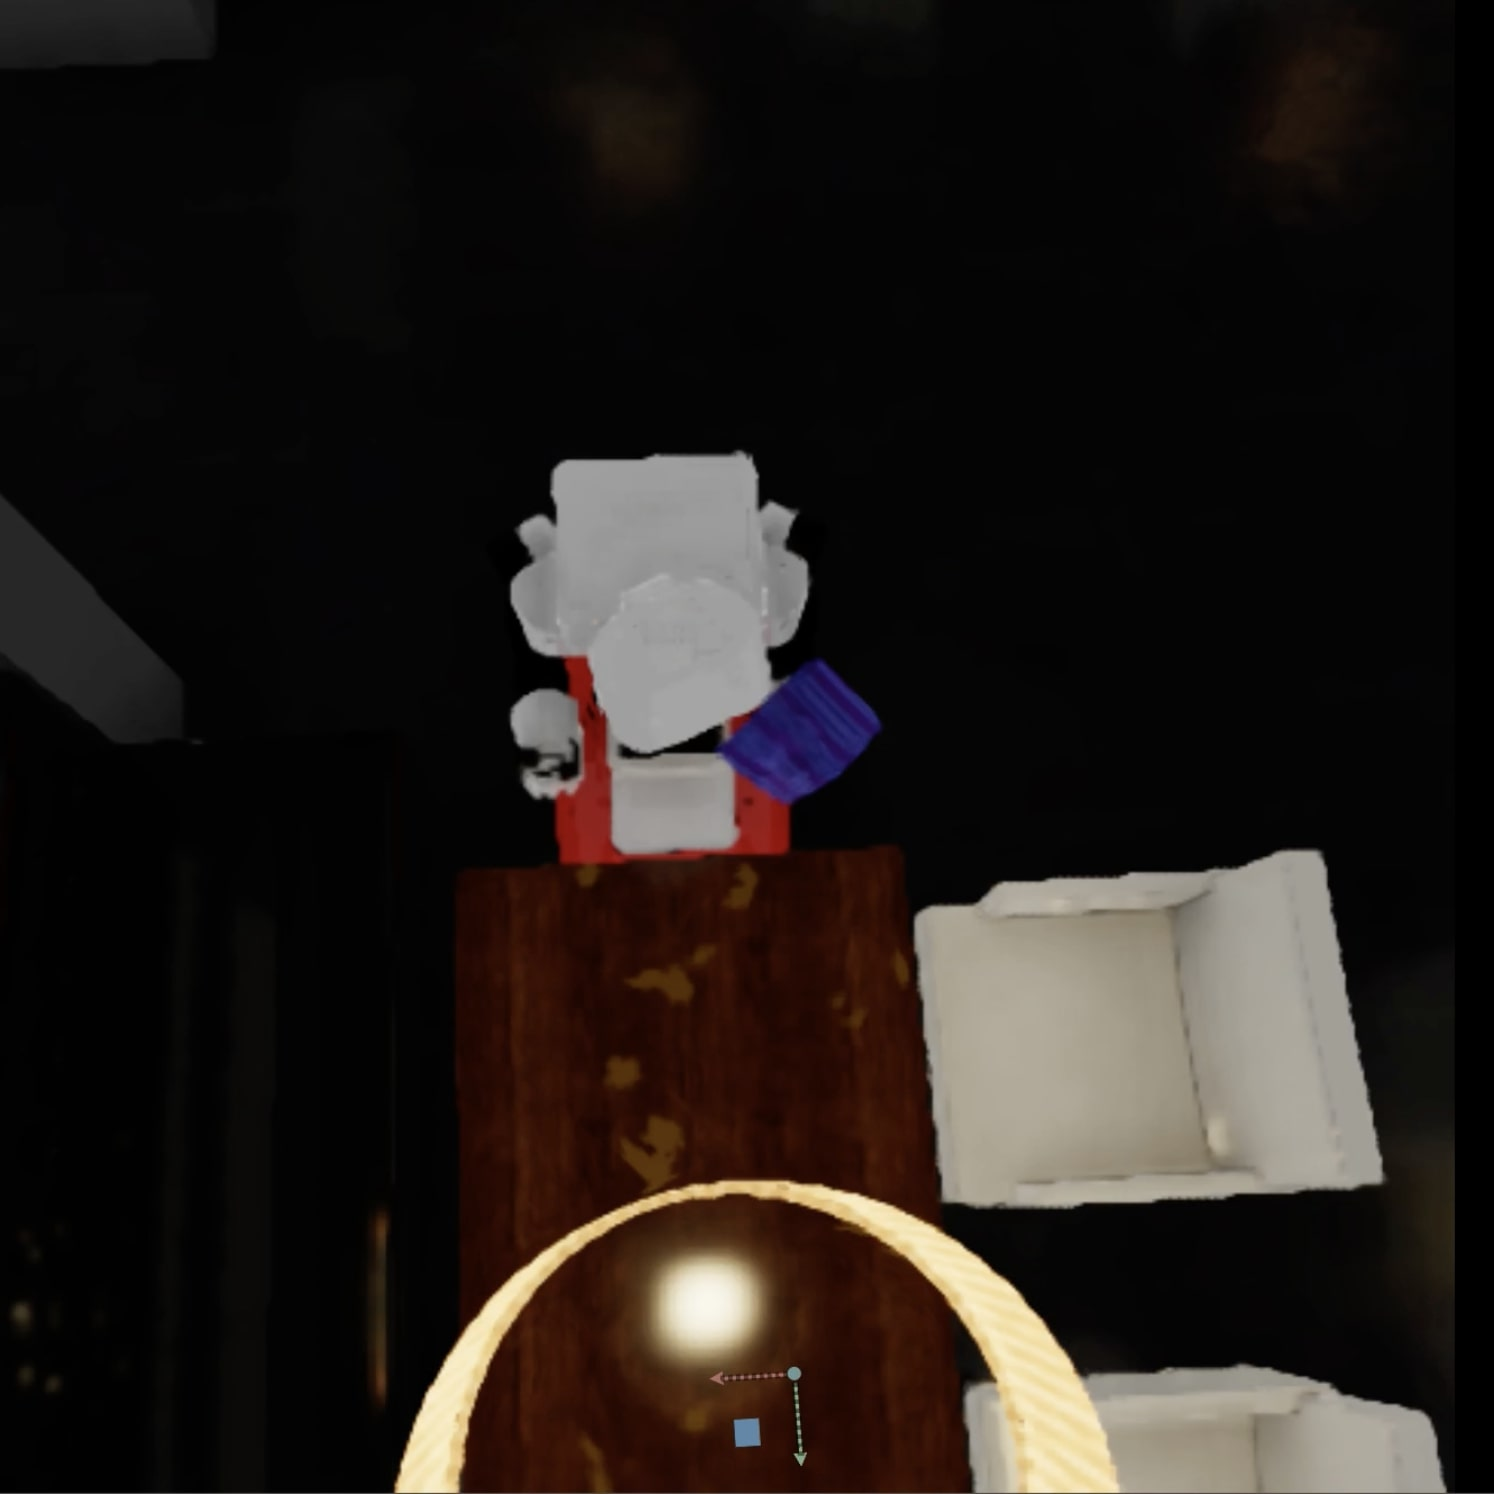
\includegraphics[trim=0 200 0 200,clip,width=0.33\linewidth]{figures/baseline_appendix/wipe_1}%
\hfill%
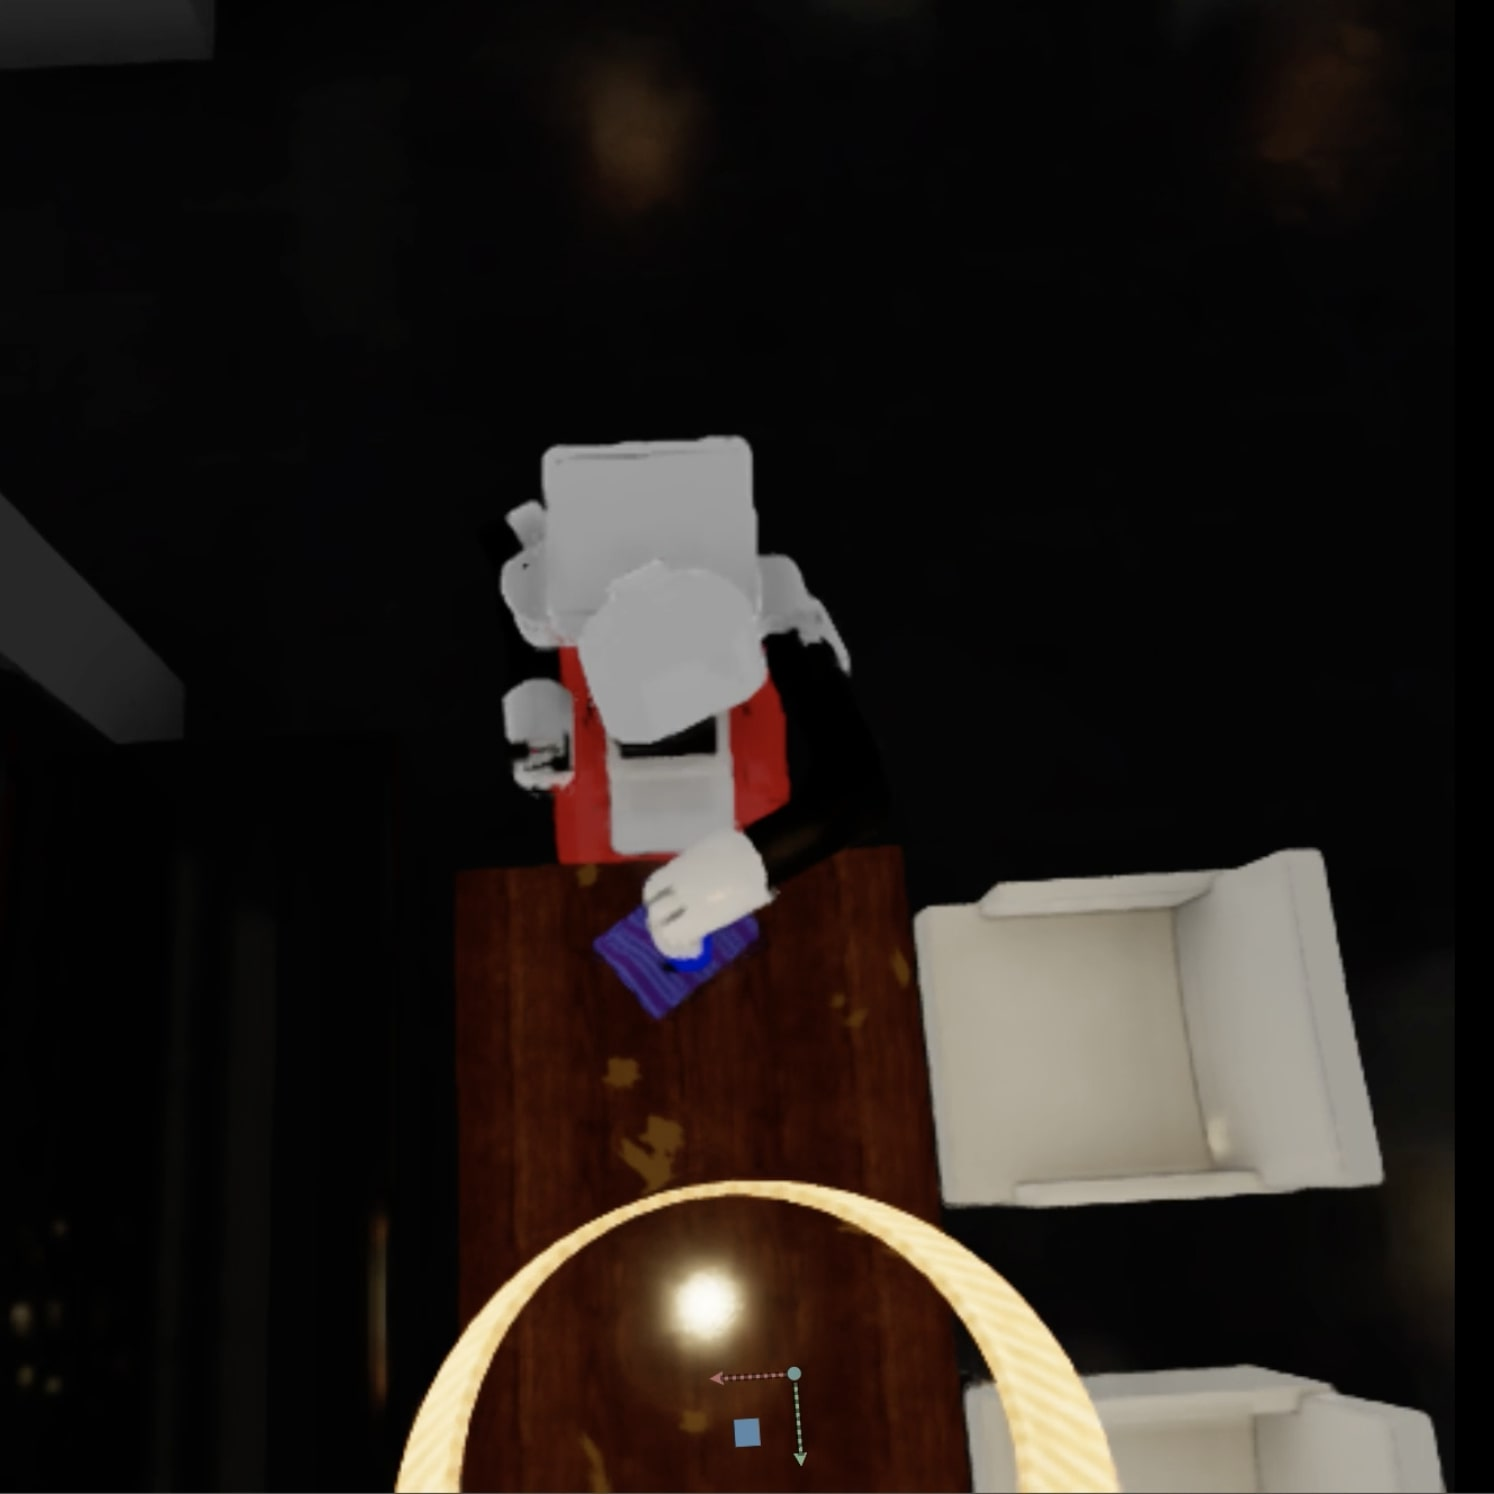
\includegraphics[trim=0 200 0 200,clip,width=0.33\linewidth]{figures/baseline_appendix/wipe_2}%
\hfill%
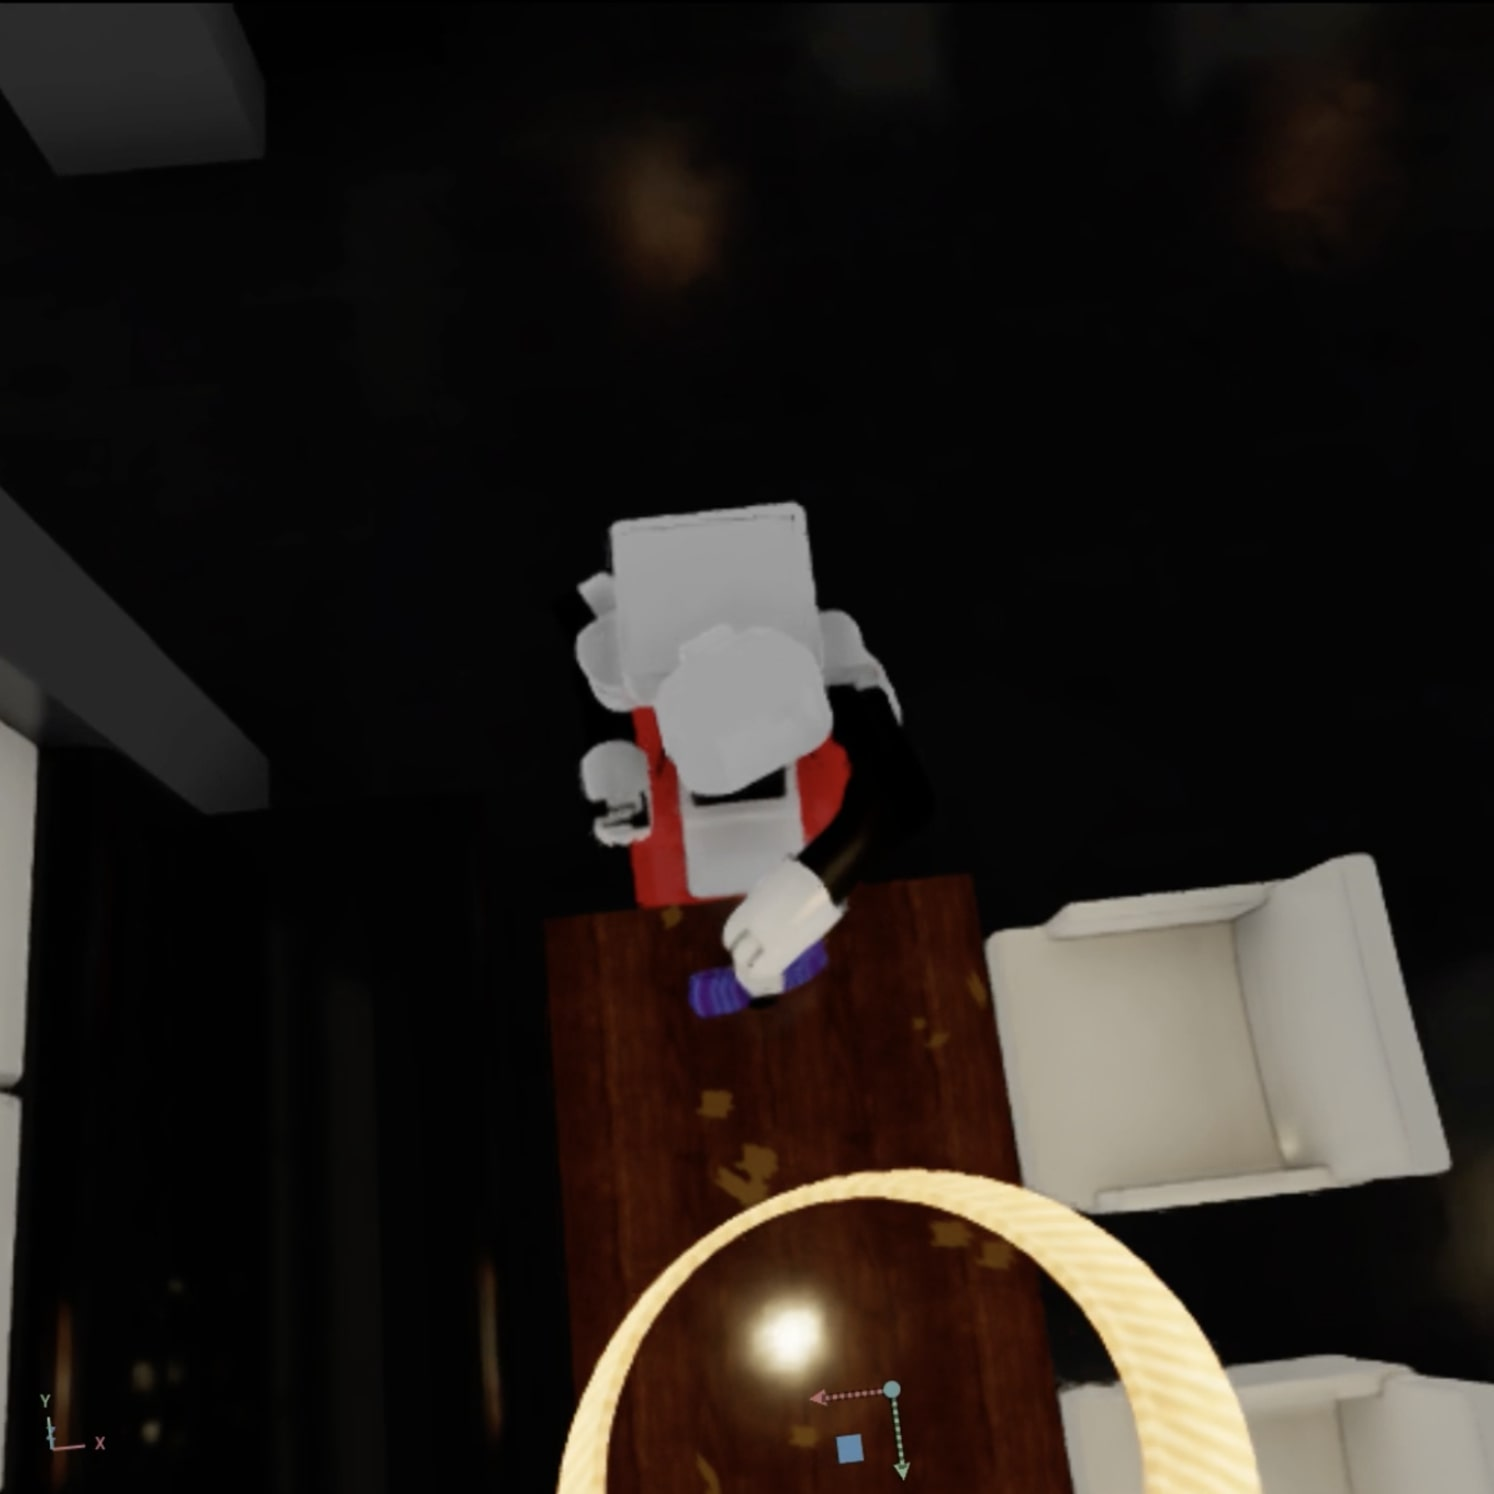
\includegraphics[trim=0 200 0 200,clip,width=0.33\linewidth]{figures/baseline_appendix/wipe_3}
}%
\vspace{-5pt}%
\caption{\texttt{wipe}}%
\vspace{10pt}%
\end{subfigure}
\caption{Overview of all the high-level action primitives with the pre-conditions (left), post-conditions (right), and intermediate states (middle) during execution.
% \roberto{consider taking the images of wipe with more lights, it is hard to see. and the robot is gone in the last image}
}
\label{fig:appendix_high_level_planner}
\end{figure}


\subsection{Additional Metrics: success score Q}
The success score Q \cite{srivastava2021behavior} for each task is reported in Table~\ref{tab:baseline_q_score}. We observe the same trend in Q as in the success rate. This is another indication of the effectiveness of our approach.
\begin{table}[h!]
    \centering
    \resizebox{\textwidth}{!}{\begin{tabular}{l|cc|ccc}
    \toprule
    \multicolumn{1}{c|}{\multirow{2}{*}{Method}} & \multicolumn{2}{c|}{Policy Features} & \multicolumn{3}{c}{Success score Q} \\
    \multicolumn{1}{c|}{} & Primitives & History & \texttt{StoreDecoration} & \texttt{CollectTrash} & \texttt{CleanTable} \\ \midrule
    \rlvmc & \textcolor{red}\faTimes & \textcolor{red}\faTimes & $0.0 \pm 0.0$ & $0.0 \pm 0.0$ & $0.0 \pm 0.0$ \\
    \rlprim & \textcolor{indiagreen}\faCheck & \textcolor{red}\faTimes & $0.50 \pm 0.05$ & $0.49 \pm 0.04$ & $0.77 \pm 0.08$ \\
    \rlprimhist & \textcolor{indiagreen}\faCheck & \textcolor{indiagreen}\faCheck & $0.59 \pm 0.03$ & $0.68 \pm 0.02$  & $0.88 \pm 0.02$ \\ \bottomrule
    \end{tabular}
    }
    \caption{Performance of three baseline methods, in terms of the success score Q.}
    \label{tab:baseline_q_score}
\end{table}


\begin{figure}
    \centering
    \begin{tabular}{cc}        
        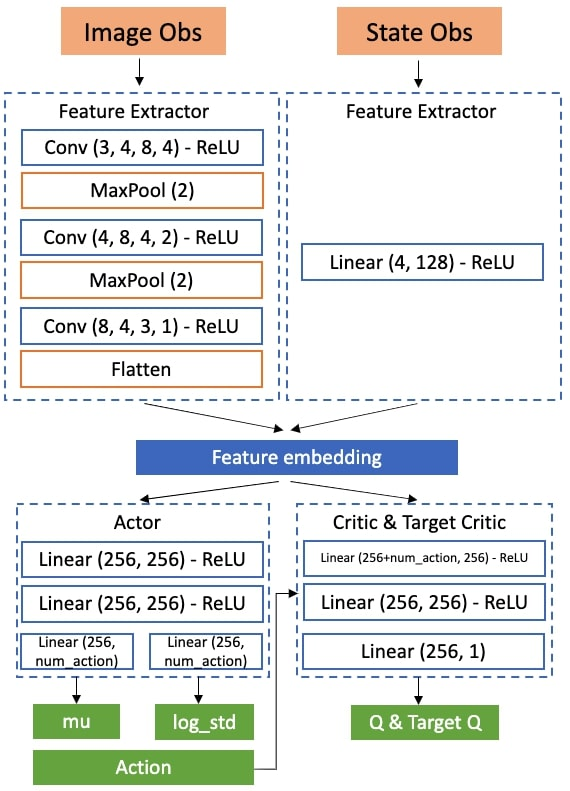
\includegraphics[width=0.45\linewidth]{figures/baseline_appendix/sac} &
        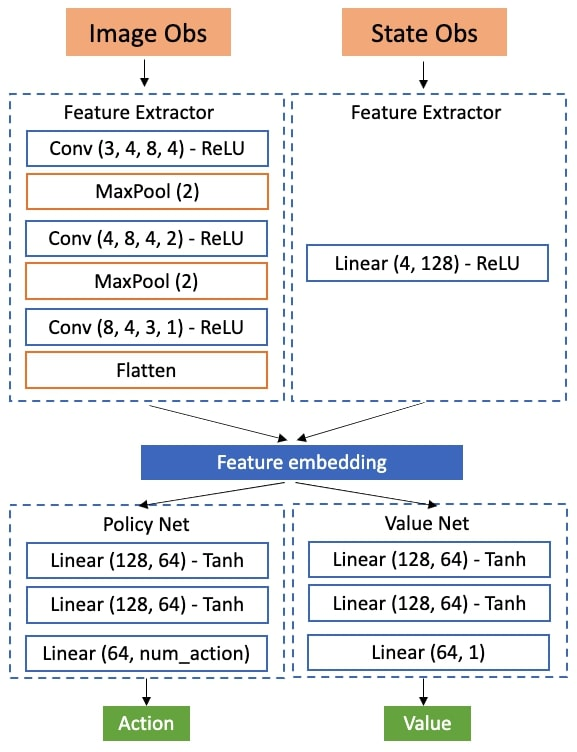
\includegraphics[width=0.45\linewidth]{figures/baseline_appendix/ppo} \\
        a) SAC Architecture & b) PPO Architecture \\
    \end{tabular}
    \caption{%\todo{VMC polict architecture} 
    Policy architecture of SAC (\rlvmc) and PPO (\rlprim and \rlprimhist). The policy maps egocentric visual observations and proprioceptive information into an action that controls the robot base, arm, and gripper. PPO outputs a discrete high-level action primitive while SAC outputs a continuous low-level joint control directly.%\roberto{make jpeg or even better, export the original as vectorgraphics/pdf}
    }
    \label{fig:appendix_ppo_vmc_arch}
\end{figure}



% \begin{figure*}[t]
% \centering
% \begin{minipage}[c]{\linewidth}
% \centering
%     \renewcommand\tabcolsep{0.5pt}
%     \begin{tabular}{ccc}
%         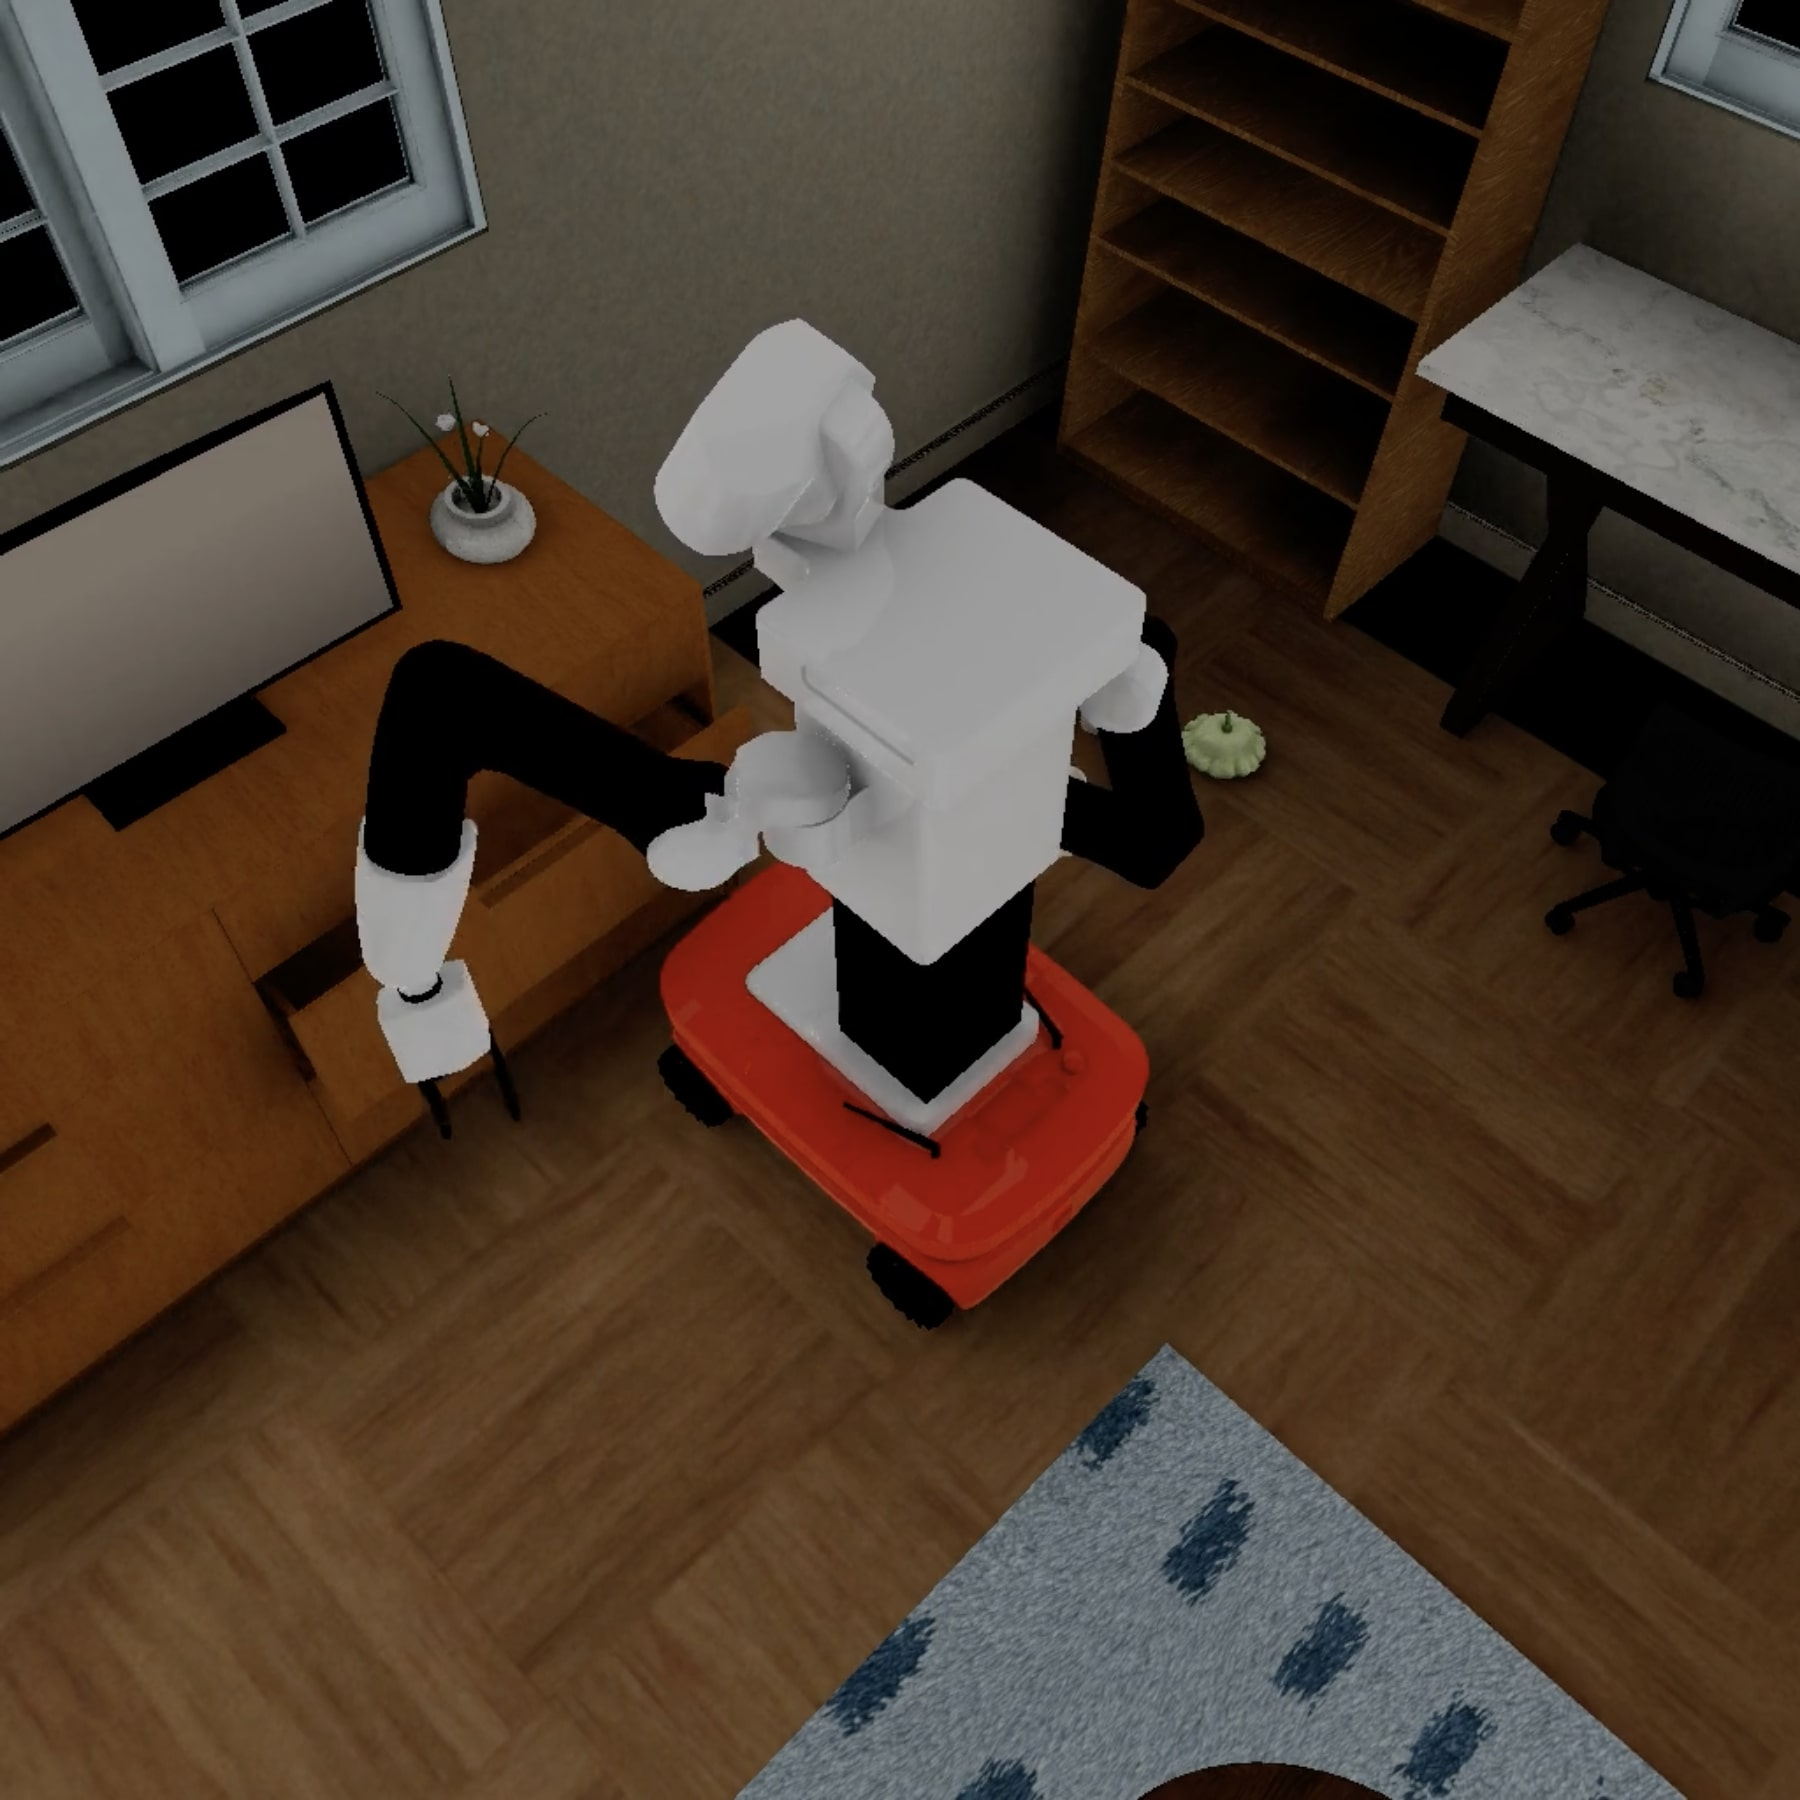
\includegraphics[width=0.3\linewidth]{figures/baseline_appendix/store_decoration_1.png}&
%         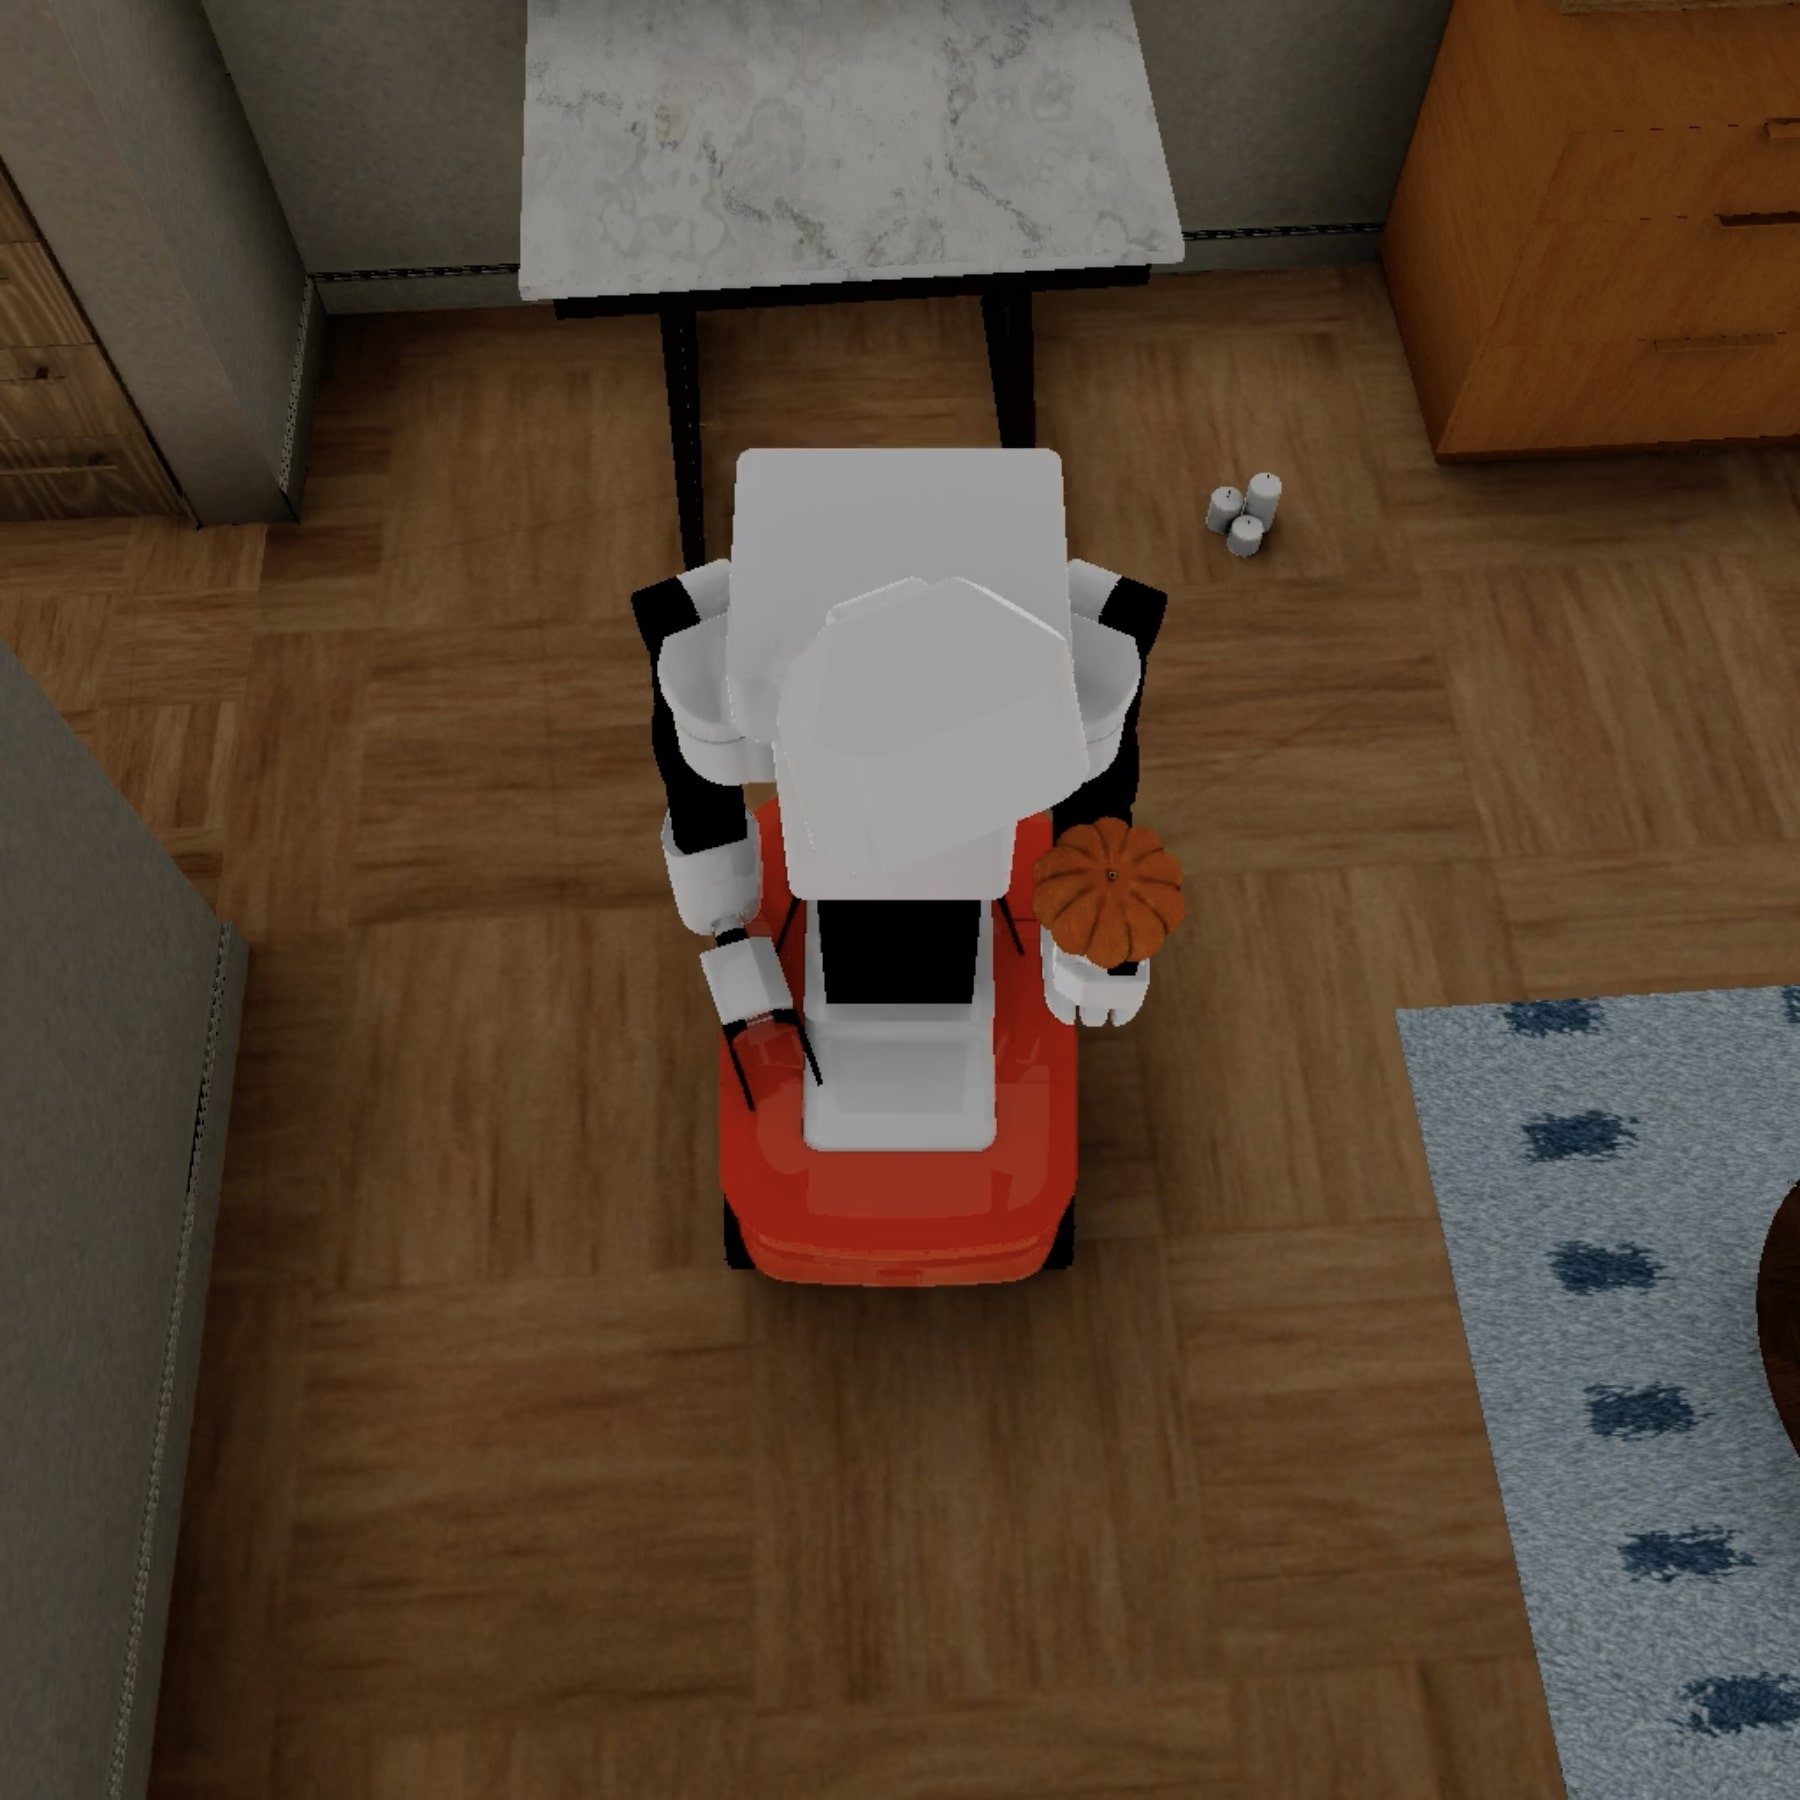
\includegraphics[width=0.3\linewidth]{figures/baseline_appendix/store_decoration_2.png}&
%         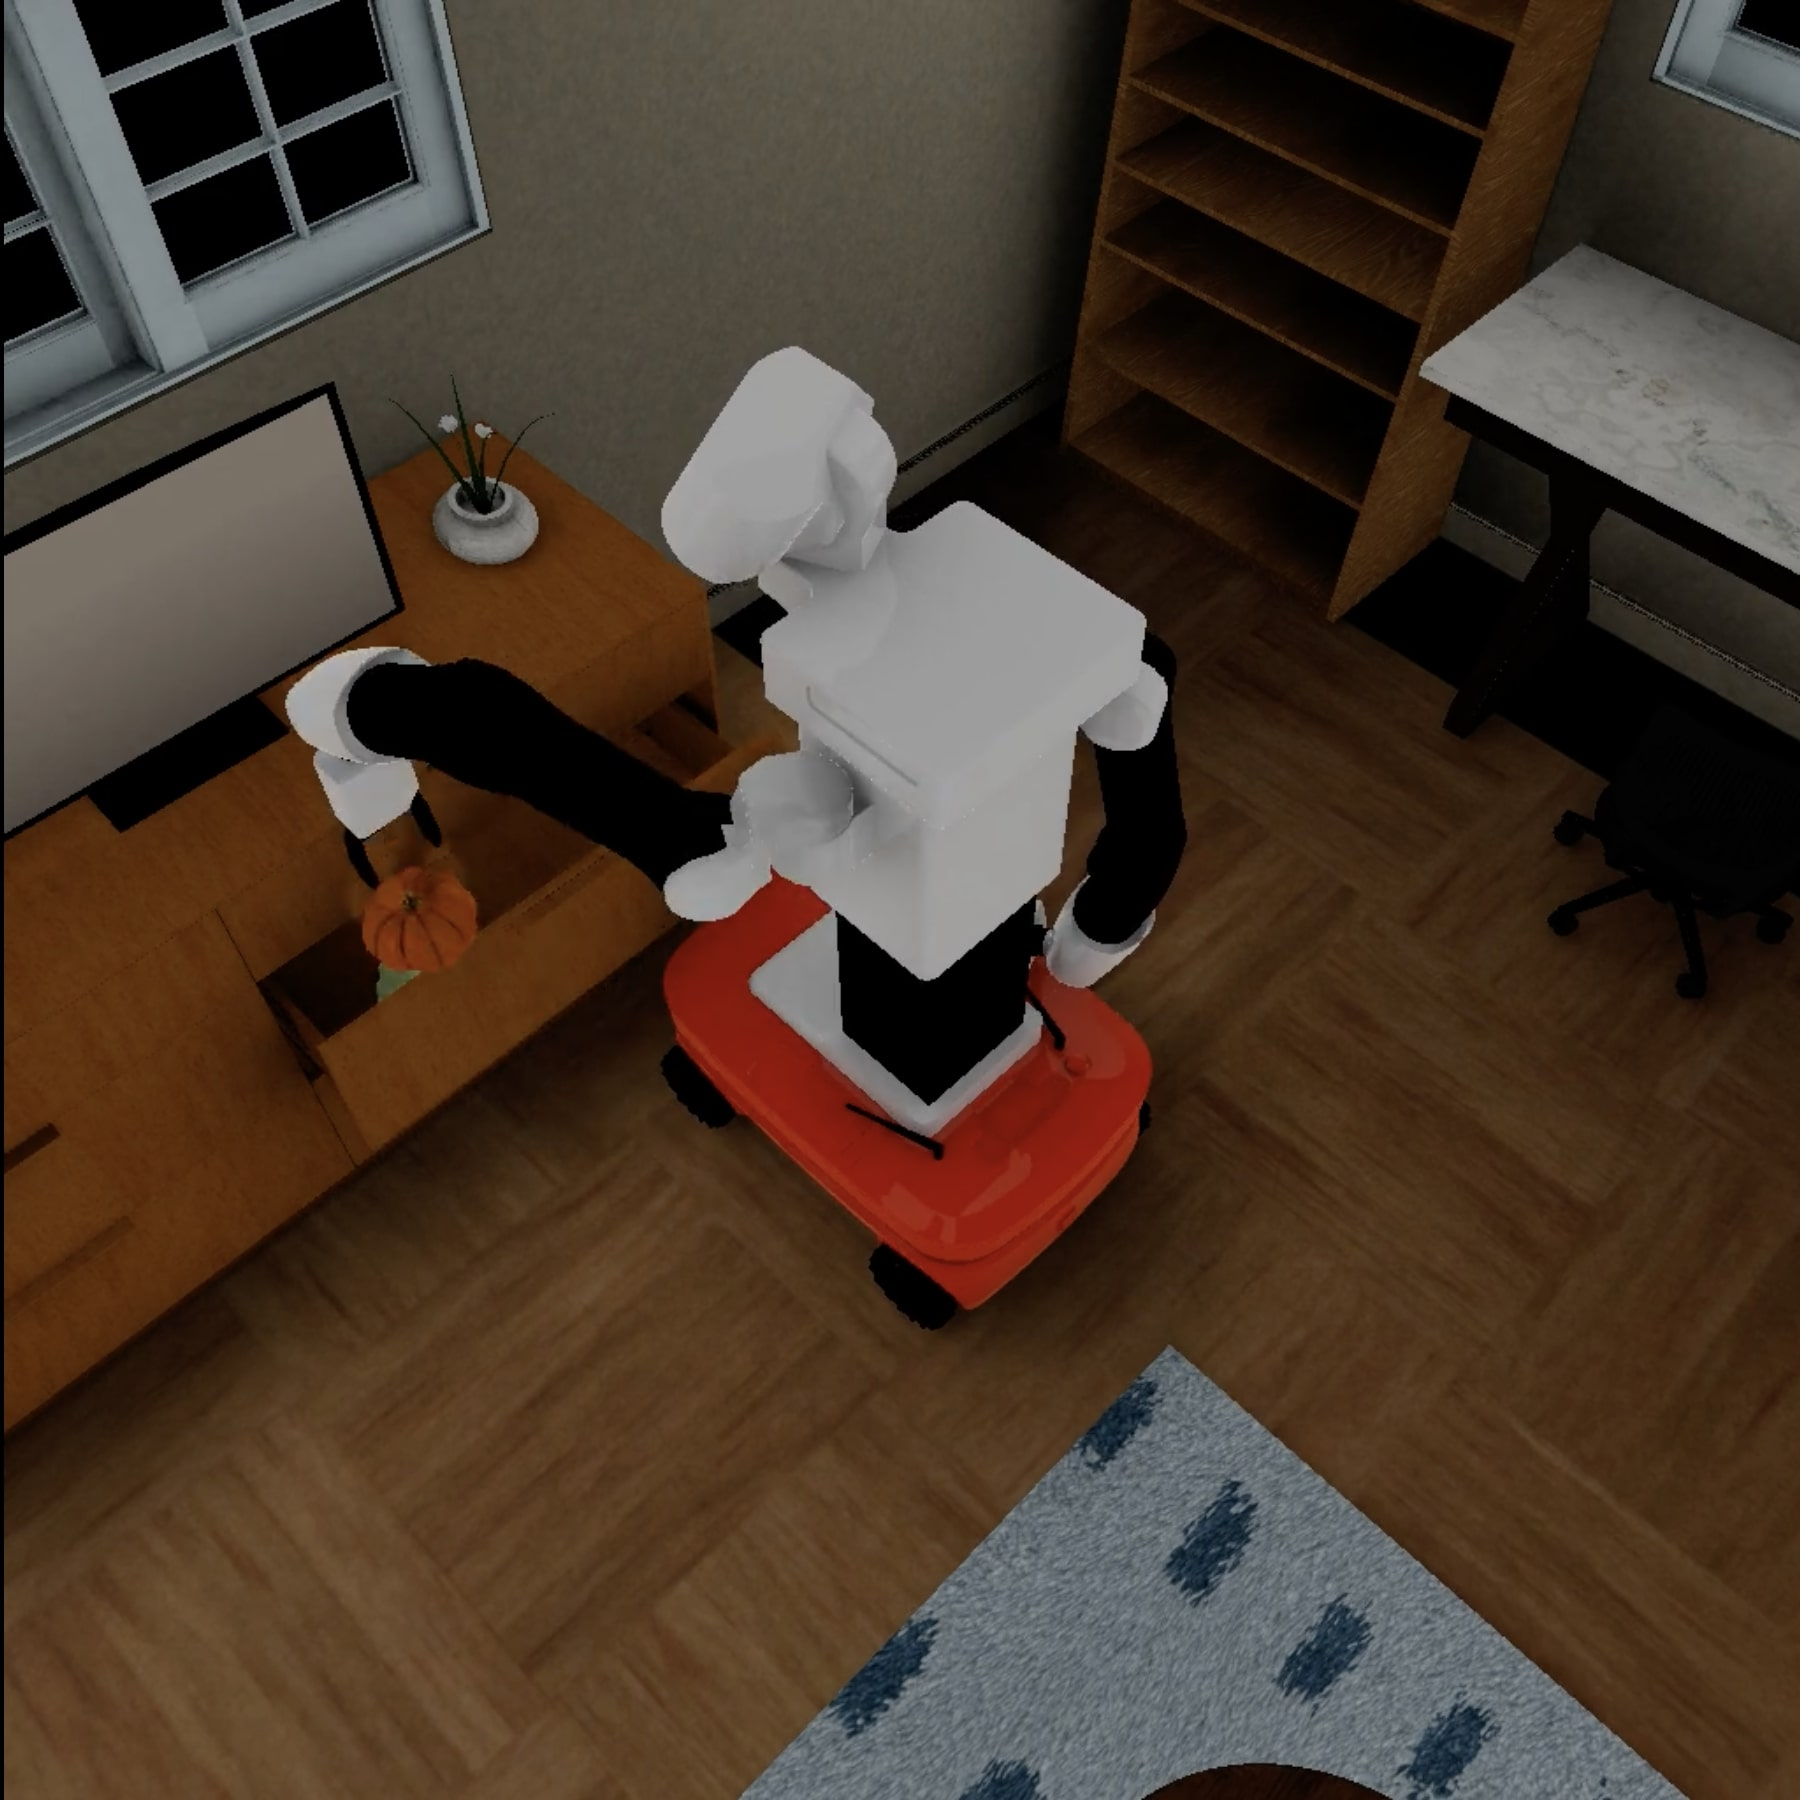
\includegraphics[width=0.3\linewidth]{figures/baseline_appendix/store_decoration_3.png}\\
%         & a) Store Decoration & \\
%         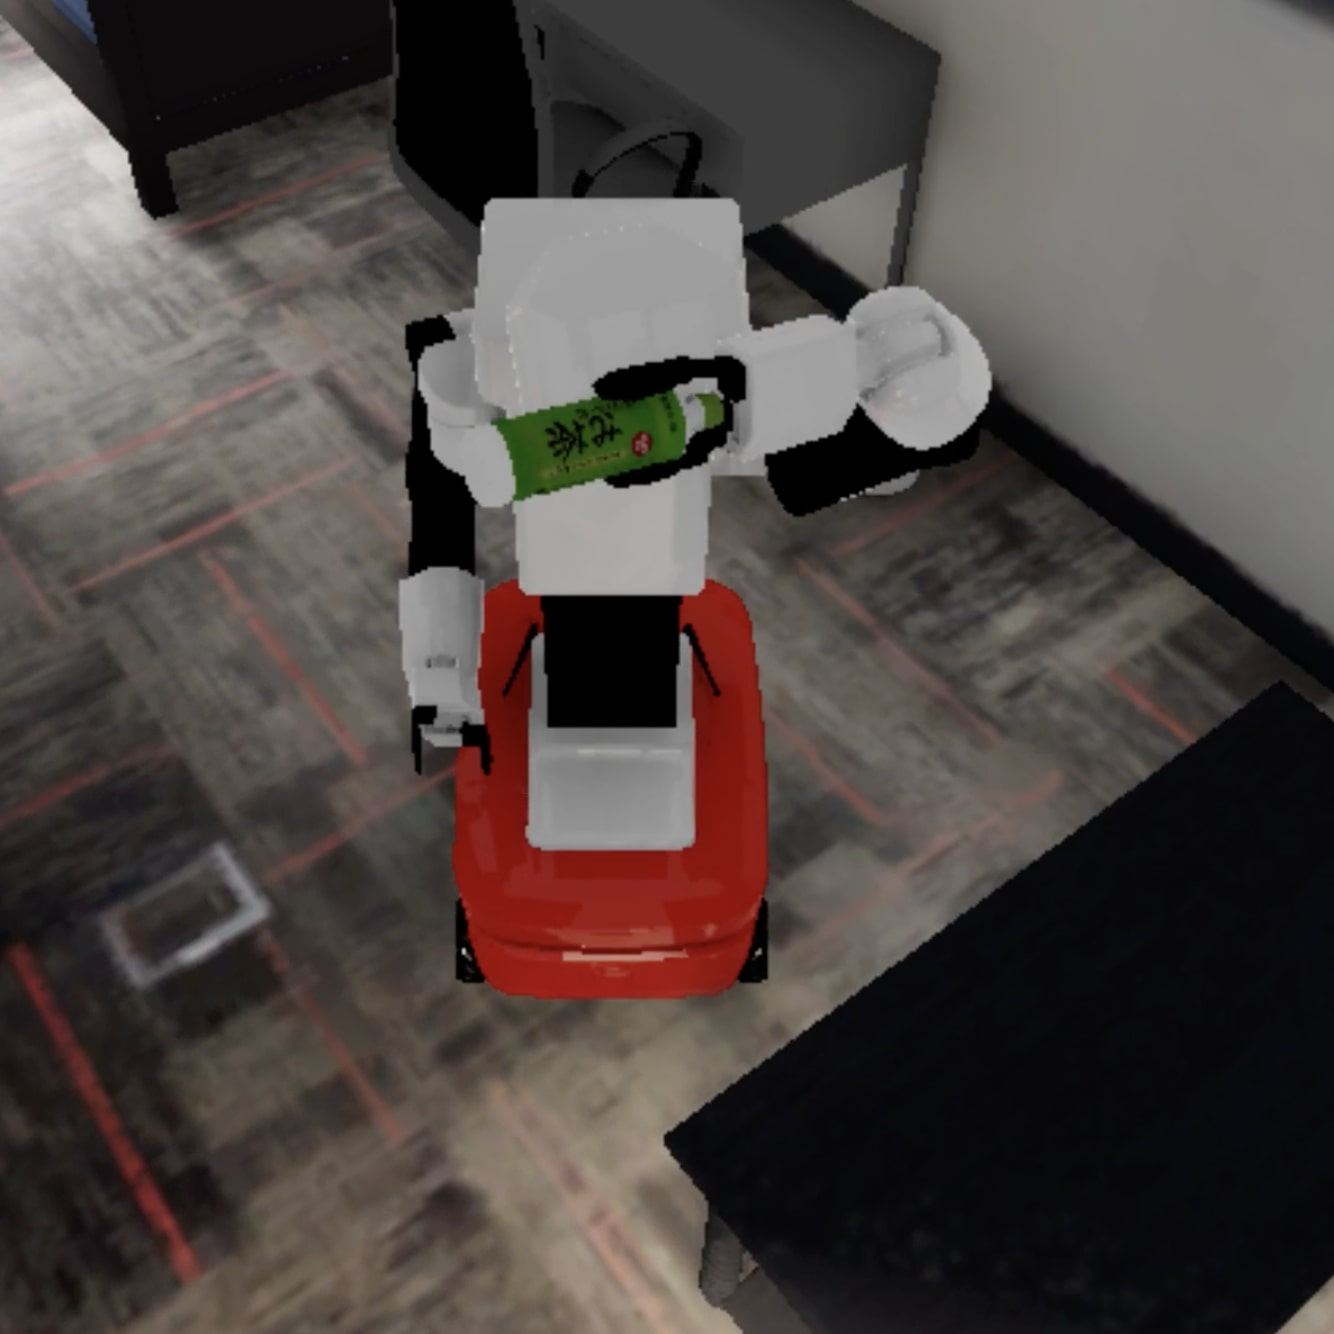
\includegraphics[width=0.3\linewidth]{figures/baseline_appendix/collect_trash_1.png}&
%         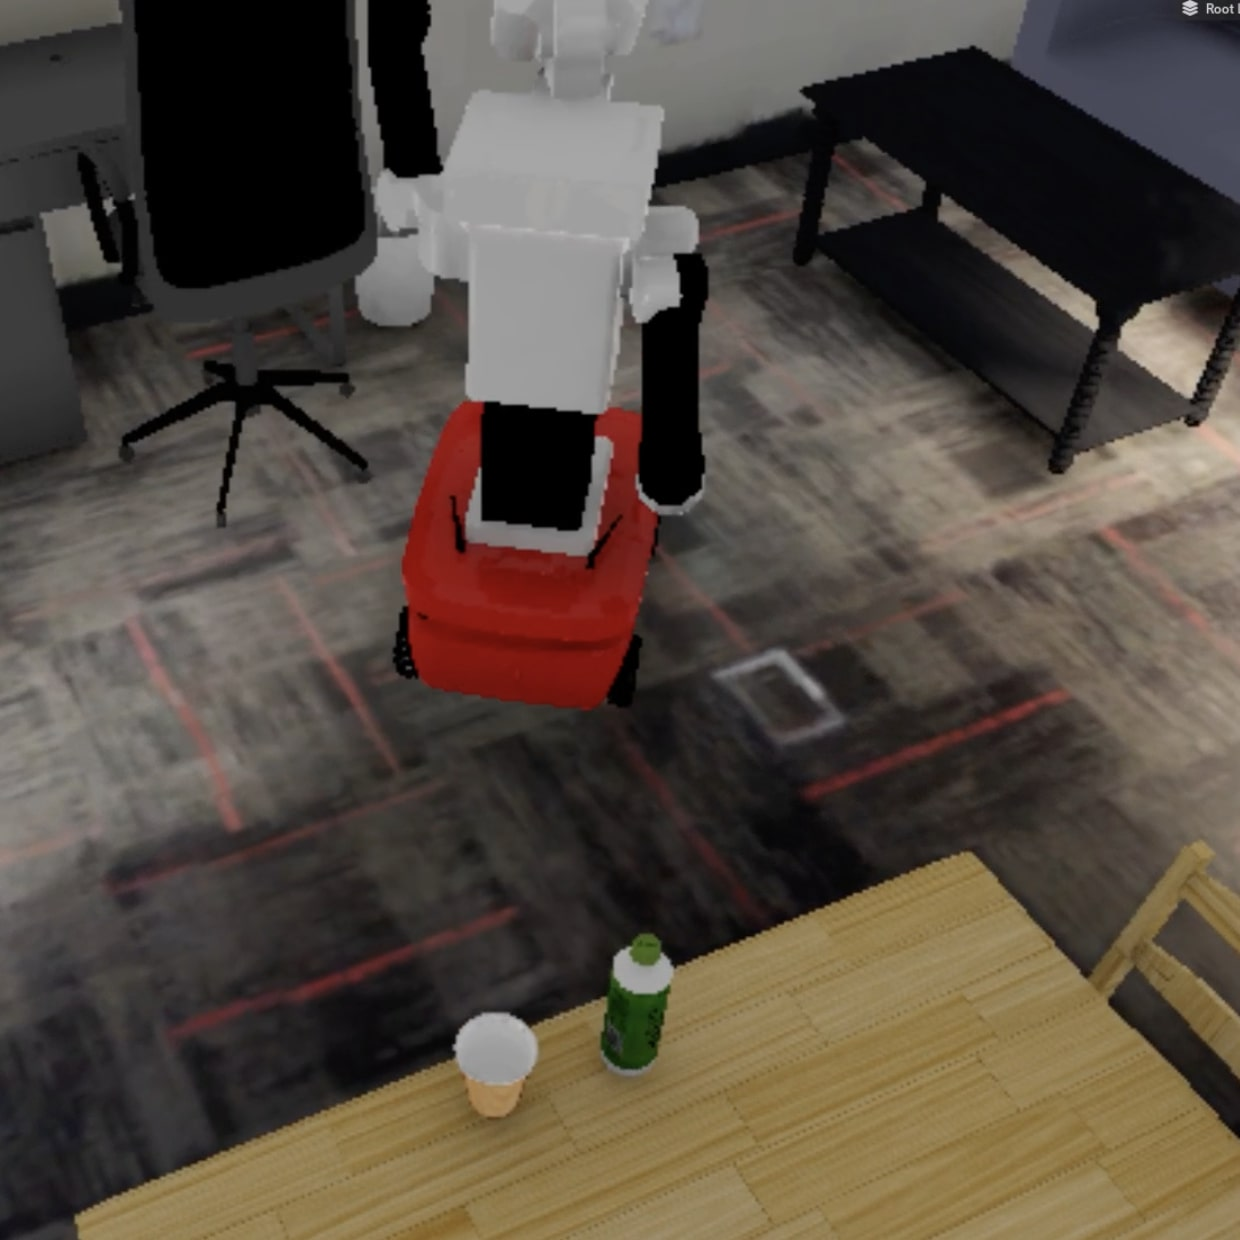
\includegraphics[width=0.3\linewidth]{figures/baseline_appendix/collect_trash_2.png}&
%         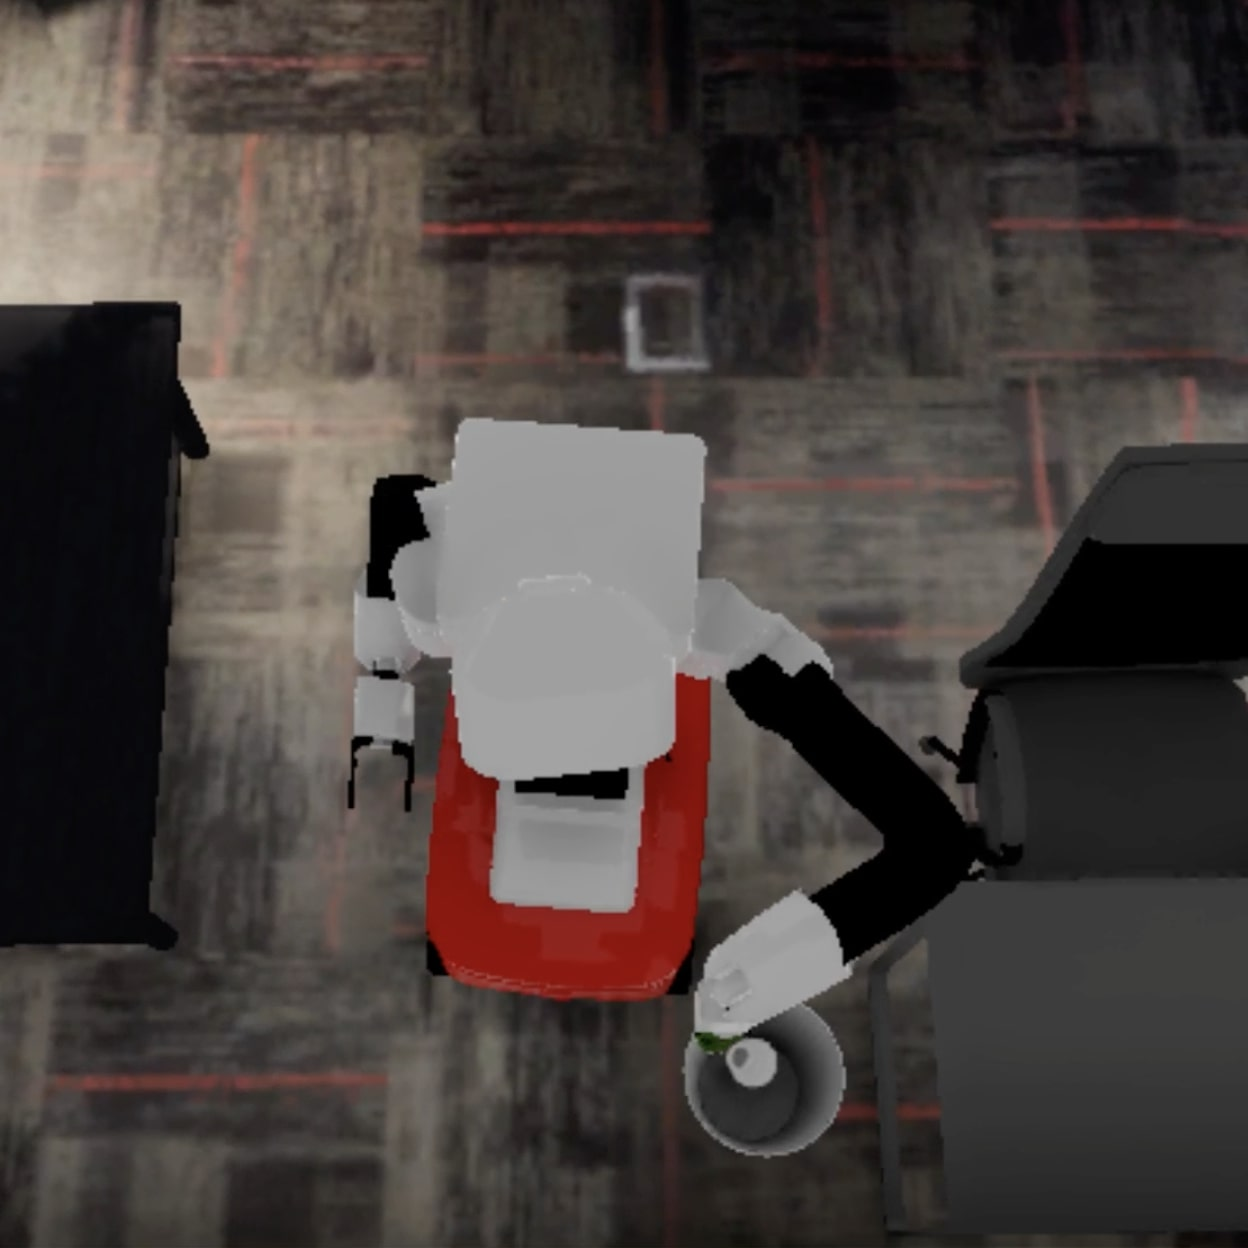
\includegraphics[width=0.3\linewidth]{figures/baseline_appendix/collect_trash_3.png}\\
%         & b) Collect Trash & \\
%         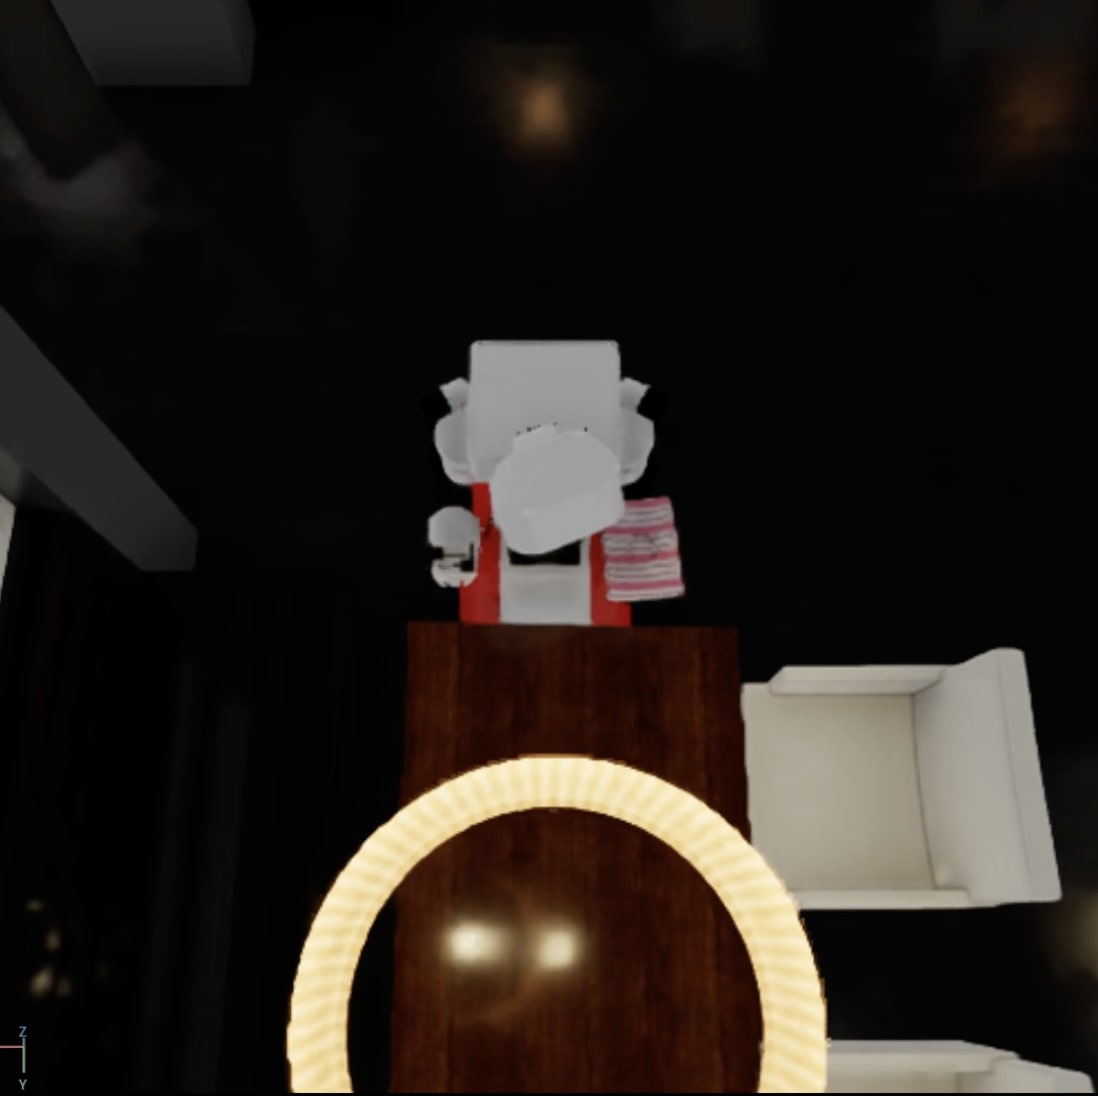
\includegraphics[width=0.3\linewidth]{figures/baseline_appendix/clean_table_1.png}&
%         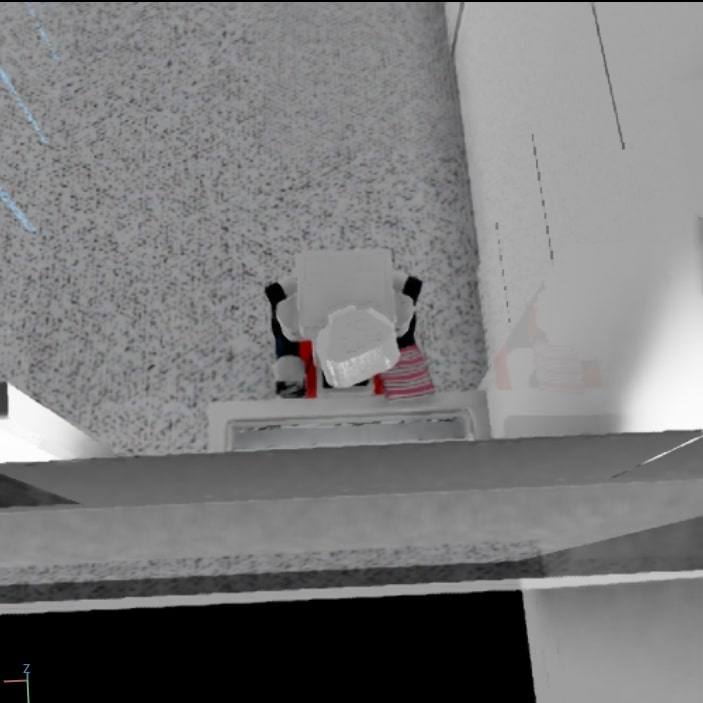
\includegraphics[width=0.3\linewidth]{figures/baseline_appendix/clean_table_2.png}&
%         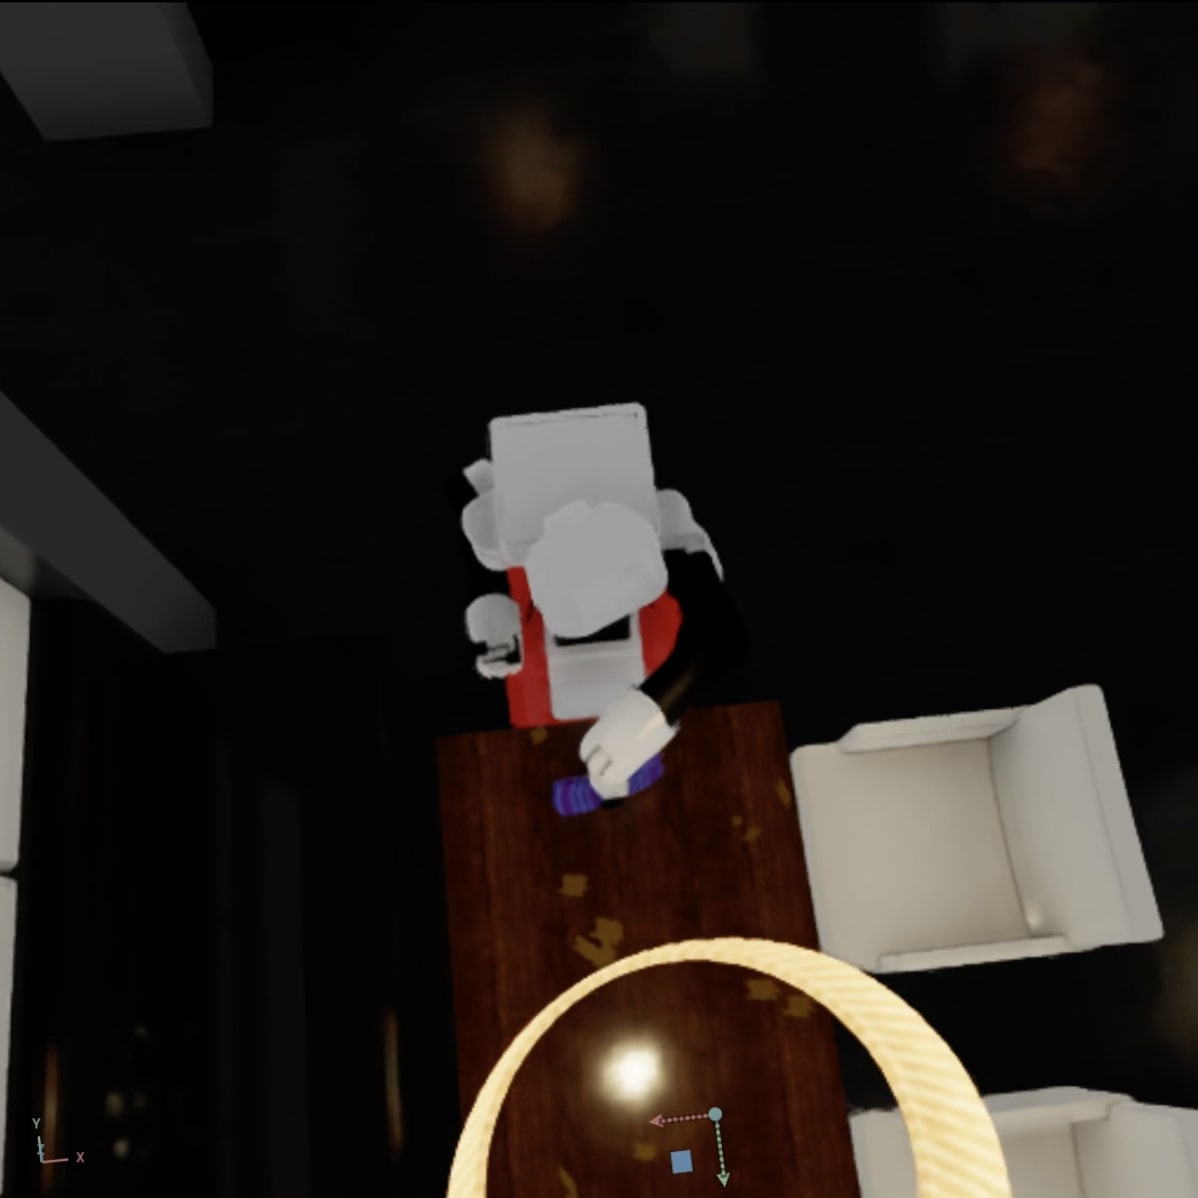
\includegraphics[width=0.3\linewidth]{figures/baseline_appendix/clean_table_3.png}\\
%         & c) Clean Table & \\
%     \end{tabular}
%     \caption{Overview of three tasks: \texttt{Store\_Decoration}, \texttt{Collect\_Trash}, and \texttt{Clean\_Table}.}
%     \label{fig:appendix_task}
% \end{minipage}
% \end{figure*}
\section{Details of the Real-World Setup}
\label{as:s2r}

\paragraph{Scene.} Our real-world experiments take place in a mockup studio-apartment in our lab that includes a bedroom, living room, and dining area. 
This real-world scene was modeled with a digital counterpart in simulation for \benchmark: the \texttt{mockup\_apt} scene. Fig.~\ref{fig:sim2real_setup} depicts both real and digital twin side-by-side. The digital model has been created by first, scanning the real-world apartment using a phone and commercial software~\cite{scaniverse}, then, replacing and projecting the texture of walls, floors, and ceilings, and finally, replacing the existing objects with 3D models from our \dataset. This process should minimize the effect caused by differences between the real world and the 3D model. The simulated and the real robot use the same 2D map of the scene for localization. In this way, 2D locations in the real world correspond to the same 2D locations in simulation. 

\paragraph{Robot platform.} We use in our experiments a Tiago++ model from PAL Robotics, with an omnidirectional base, two 7-degrees-of-freedom arms with parallel-yaw grippers, a 1-degree-of-freedom prismatic torso, two SICK LiDAR sensors (back and front of the base), and an ASUS Xtion RGB-D camera mounted on the robot's head, which can be controlled in yaw and pitch.
All sensors and actuators are connected through the Robot Operating System, ROS~\cite{quigley2009ros}. The code runs on a laptop with an Nvidia GTX 1070 that sends the commands to the onboard robot computer to be executed.

\paragraph{Action primitives on the real robot.} We implemented a version of the action primitives \texttt{navigate}, \texttt{pick} and \texttt{place} on the real robot similar to their implementation in \simulator. For navigation, we use a 2D sampling-based motion planner on the 2D map we use for localization and that has been created from the 3D model of the apartment. For manipulation in the real world, we need to obtain the parameters necessary to plan the manipulation primitives (\texttt{pick} and \texttt{place}) from the sensor signals. To do that, we first obtain detections from a YOLO v3~\cite{redmon2018yolov3} object detector on the RGB images from the robot's camera. If the robot attempts to execute an action primitive on an object that has not been detected, we return failure (\textit{Object Detection Failure} in our analysis). If the object to manipulate has been detected, we query the pixels in the depth map corresponding to the 21$\times$21 window at the center of the detection bounding box, and use this information to compute the centroid of the corresponding 3D points. This location will be used as an object location for grasping or placing. This information is enough to create a sequence of paths using a sampling-based motion planner (RRT~\cite{kuffner2000rrt}) similar to the ones used in simulation. The motion planner uses a voxel representation of the scene obtained from the depth sensor.

\paragraph{Experimental setup.} We randomized three parameters in our real robot experiments: the initial location of the robot (chosen from the three possible activity locations), the positions of the objects on the table, and the orientations of the objects (upright or lying down). The experiment runs cover uniformly these parameters. Additionally, for vision-based policies, we evaluated two lighting conditions: full lighting (including the ceiling) and only lamps.
Failures are defined as follows:
Motion planning failures occurred when the robot was unable to plan an end effector trajectory to complete the action primitive. This includes failures caused by navigation noise, where after navigating to the task location, the robot was too far away from the target object to execute the pick or place action. 
Grasping failures include errors that occurred during the execution of the grasp such as pushing the object off the table while attempting a grasp or losing the object because it slips out, as well as the robot dropping the object after grasping it.
Placing failures include the robot dropping the object in the wrong location. 
Object detection failures primarily resulted from our object detector, YOLO v3~\cite{redmon2018yolov3}, failing to detect the object to interact with; a second, less common, object detection failure corresponds to the depth camera returning invalid measurements for the detected object. 
Finally, we consider policy failures when the policy selects the same invalid action three times in a row, e.g., requesting to navigate to the bin when it is already in front of the bin. The main policy error corresponds to the policy repeatedly choosing the same action primitive. We observed empirically that, even though the policy selection presents some small randomness when the policy requests the same invalid action three times in a row, most subsequent calls will be also the same invalid action and we decide to terminate early.

% \subsection{Further Characterization of the Sim-Real Gap}

% We performed additional experiments to characterize the gap between simulation and the real world. In our experiments, we navigated the robot to different locations in the \texttt{mockup\_apt} scene and collect visual sensor signals: RGB images, depth maps, and lidar measurements. We then moved the robot in simulation to the same locations and collected virtual sensor signals. Some of the images are depicted in Fig.~\ref{fig:simrealsensors}. We observe that, thanks to our highly realistic models, \simulator provides high-fidelity sensor signals that approximate correctly the real-world ones. However, some of the sources of noise in the real sensors are not modeled currently in \simulator, contributing to creating a sim-real gap, e.g., the poor dynamic range of the RGB camera, or the ``shadow'' effects in depth maps due to the projected light mechanism in the depth maps. This analysis indicates possible avenues to close further the gap between simulation and the real world, e.g., by including models of these noise sources in \simulator or with sim2real solutions to transfer the policies (e.g., domain randomization) that can overcome these differences.

% \begin{figure}[h!]
%     \centering
%     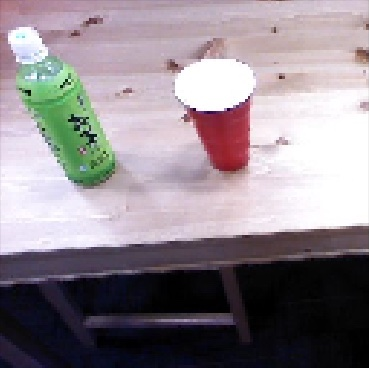
\includegraphics[width=0.31\linewidth]{figures/sim2real/rgb_kitchen_table.jpg}
%     \hfill
%     %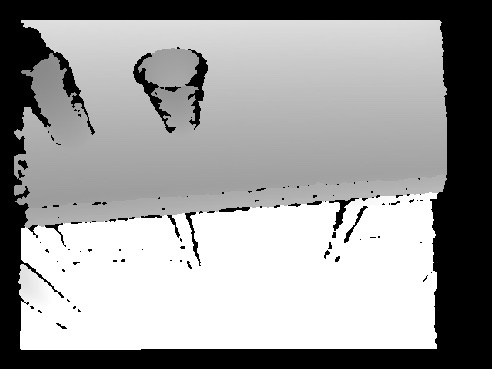
\includegraphics[width=0.31\linewidth]{figures/sim2real/d_kitchen_table.jpg}
%     %\hfill
%     %\includegraphics[width=0.31\linewidth]{example-image-c}
%     \\\vspace{3pt}
%     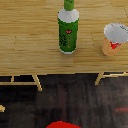
\includegraphics[width=0.31\linewidth]{figures/sim2real/sim_rgb_kitchen_table.jpg}
%     \hfill
%     %\includegraphics[width=0.31\linewidth]{example-image-b}
%     %\hfill
%     %\includegraphics[width=0.31\linewidth]{example-image-c}
%     \\\vspace{10pt}
%     \includegraphics[width=0.31\linewidth]{figures/sim2real/rgb_trash_bin.jpg}
%     \hfill
%     %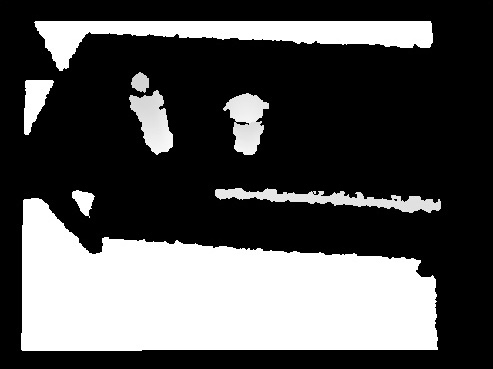
\includegraphics[width=0.31\linewidth]{figures/sim2real/d_coffee_table.jpg}
%     %\hfill
%     %\includegraphics[width=0.31\linewidth]{example-image-c}
%     \\\vspace{3pt}
%     \includegraphics[width=0.31\linewidth]{figures/sim2real/sim_rgb_trash_bin.jpg}
%     \hfill
%     %\includegraphics[width=0.31\linewidth]{example-image-b}
%     %\hfill
%     %\includegraphics[width=0.31\linewidth]{example-image-c}
% %    \caption{\textbf{Comparison between simulated and real sensor signals.} From left to right: RGB, Depth and Lidar signals in simulation (first and third rows) and from the real-world sensors (second and third rows) in two different locations of the \texttt{mockup\_apt} scene (location 1: first two rows, location 2: last two rows). Apart from some unmodeled sources of noise in the real-sensors, we observe a high realism in the signals generated in \simulator.}
%     \caption{\textbf{Comparison between simulated and real sensor signals.} RGB signals in simulation (first and third rows) and from the real-world sensors (second and third rows) in two different locations of the \texttt{mockup\_apt} scene (location 1: first two rows, location 2: last two rows). Apart from some unmodeled sources of noise in the real-sensors, we observe a high realism in the signals generated in \simulator.}
%     \label{fig:simrealsensors}
% \end{figure}

\subsection{Further Characterization of the Sim-Real Gap}

\revision{We performed additional experiments to characterize the gap between simulation and the real world. In our experiments, we moved the robot to different locations in the \texttt{mockup\_apt} scene and collected real sensor signals: RGB images, depth maps, and LiDAR measurements. We then moved the robot in simulation to the same locations and collected virtual sensor signals. Some of the images are depicted in Fig.~\ref{fig:simrealsensors}. We observe that, thanks to our highly realistic models, \simulator provides high-fidelity sensor signals that approximate the real-world ones. However, some of the sources of noise in the real sensors are not modeled currently in \simulator, contributing to a sim-real gap, e.g., the poor dynamic range of the RGB camera, or the ``shadow'' effects in depth maps due to the projected light mechanism. This analysis indicates possible avenues to further close the sensor gap between simulation and the real world, e.g., by including sensor noise models in \simulator or by leveraging sim-to-real techniques (e.g., domain randomization, system identification).}

\subsection{Additional Experiments}
\revision{
In addition to \rlprimhist, we also evaluated \rlvmc and \rlprimhist in the real world and observed a similar trend of performance in the real world as in simulation: \rlvmc < \rlprim < \rlprimhist. \rlvmc still achieves zero success because of sparse reward and exploration difficulty during training. \rlprim has worse performance than \rlprimhist: on average, the robot with \rlprimhist successfully places 0.64 cups/bottles, whereas the one with \rlprim places 0. Qualitatively, \rlprim tends to get stuck in a repetitive action loop because the agent is unaware of its action history. This preliminary result offers us some confidence that \simulator can be a reliable test bed for future sim-to-real robotics research.
}
\begin{figure}[h!]
    \centering
    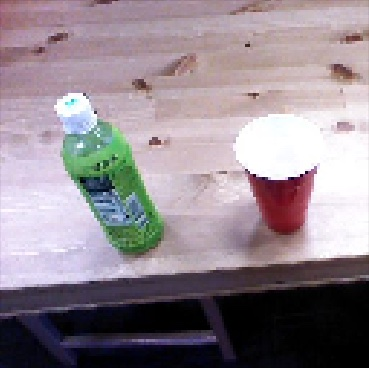
\includegraphics[width=0.31\linewidth]{figures/sim2real/rgb_real_kitchen_table.jpg}
    \hfill
    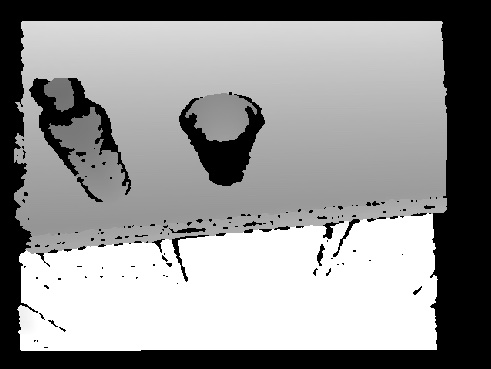
\includegraphics[width=0.31\linewidth]{figures/sim2real/depth_real_kitchen_table.jpg}
    \hfill
    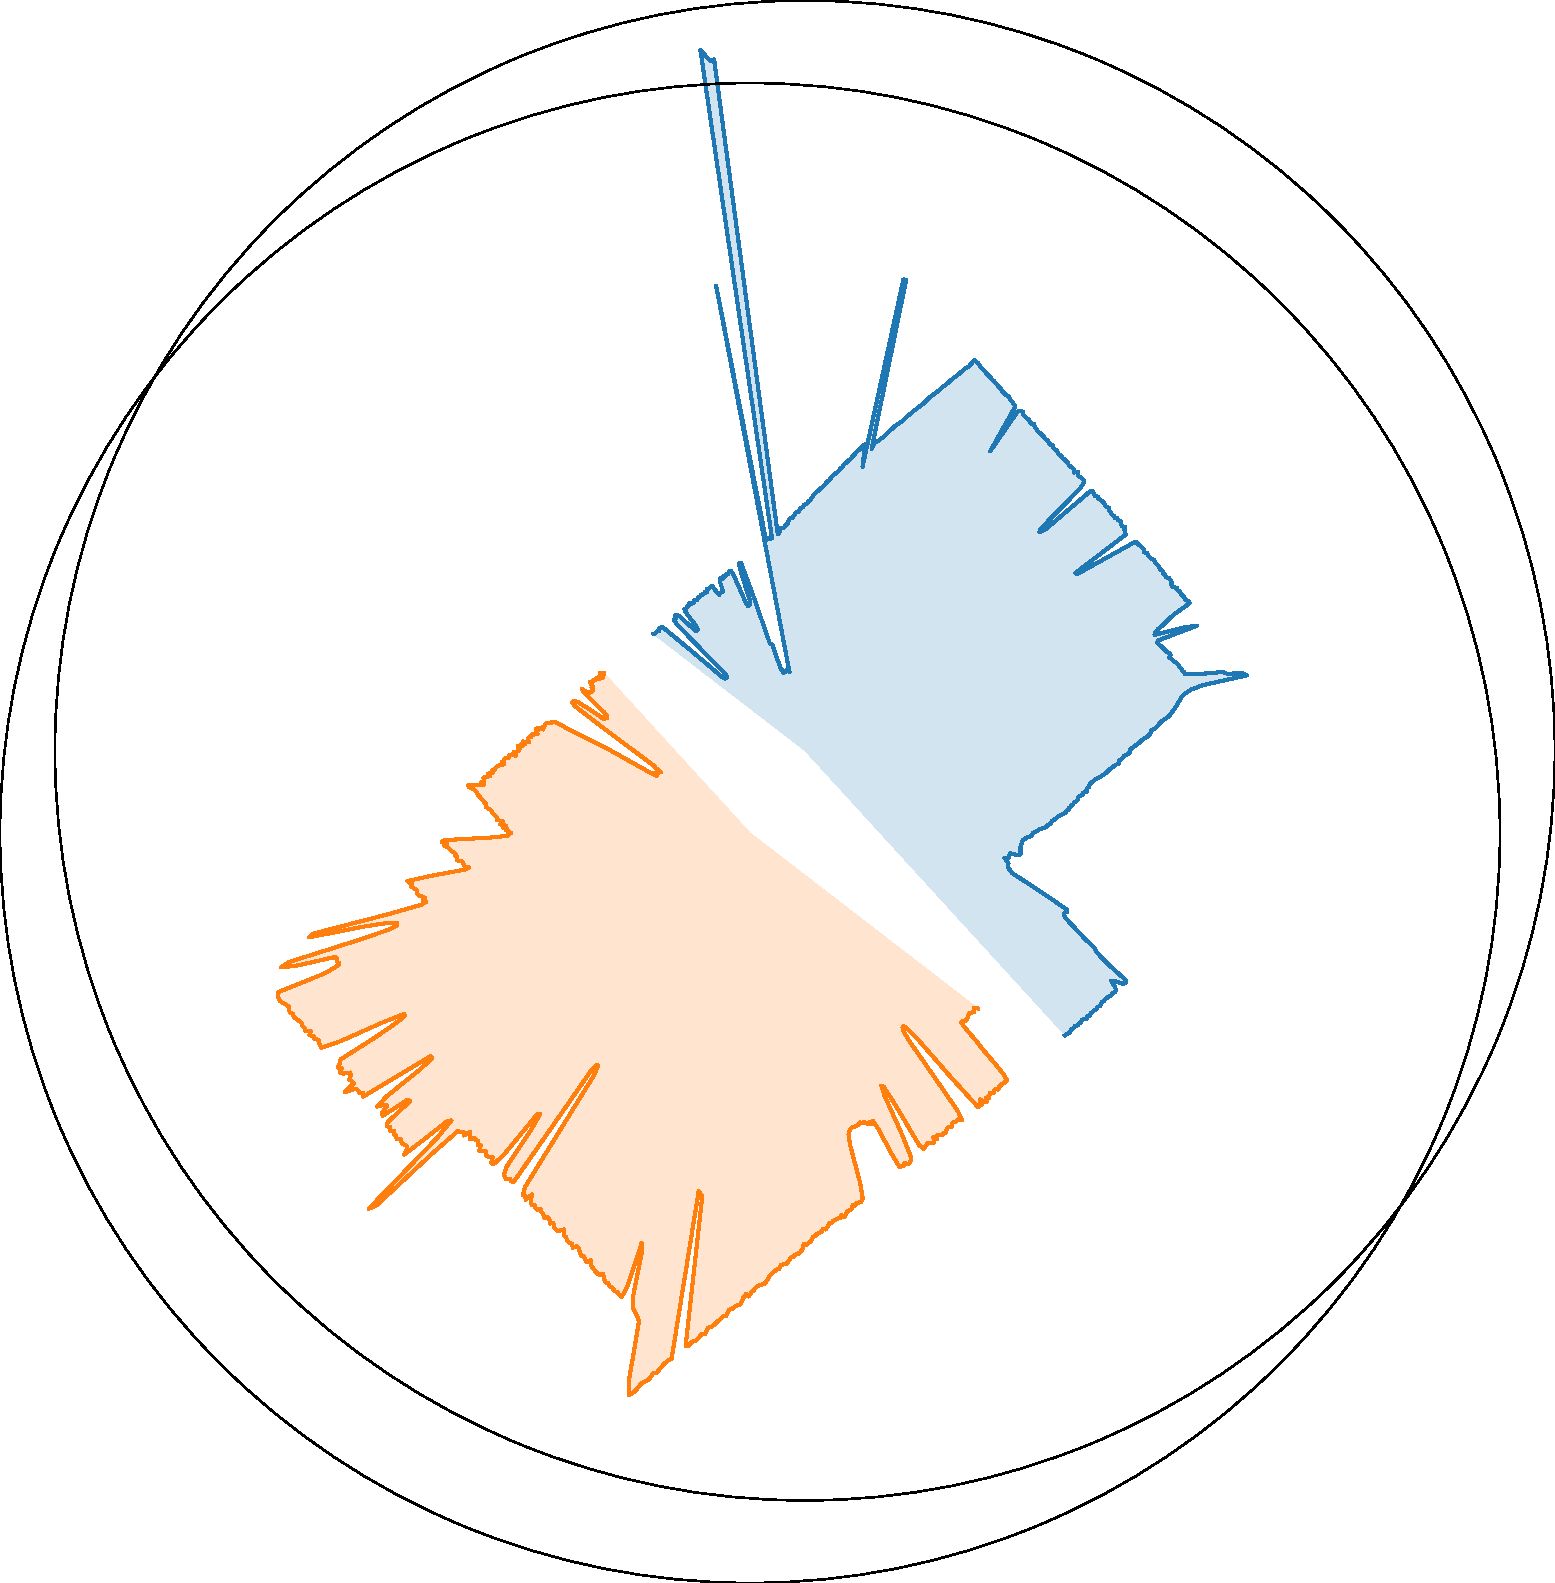
\includegraphics[width=0.31\linewidth]{figures/sim2real/lidar_real_kitchen_table}
    \\\vspace{3pt}
    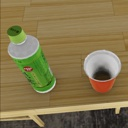
\includegraphics[width=0.31\linewidth]{figures/sim2real/rgb_sim_kitchen_table.jpg}
    \hfill
    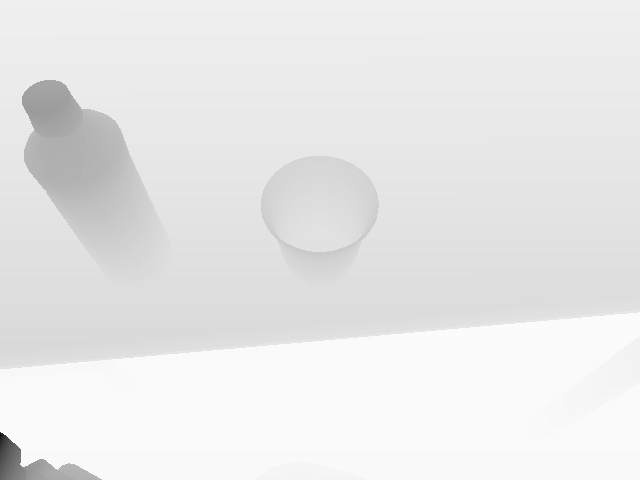
\includegraphics[width=0.31\linewidth]{figures/sim2real/depth_sim_kitchen_table.jpg}
    \hfill
    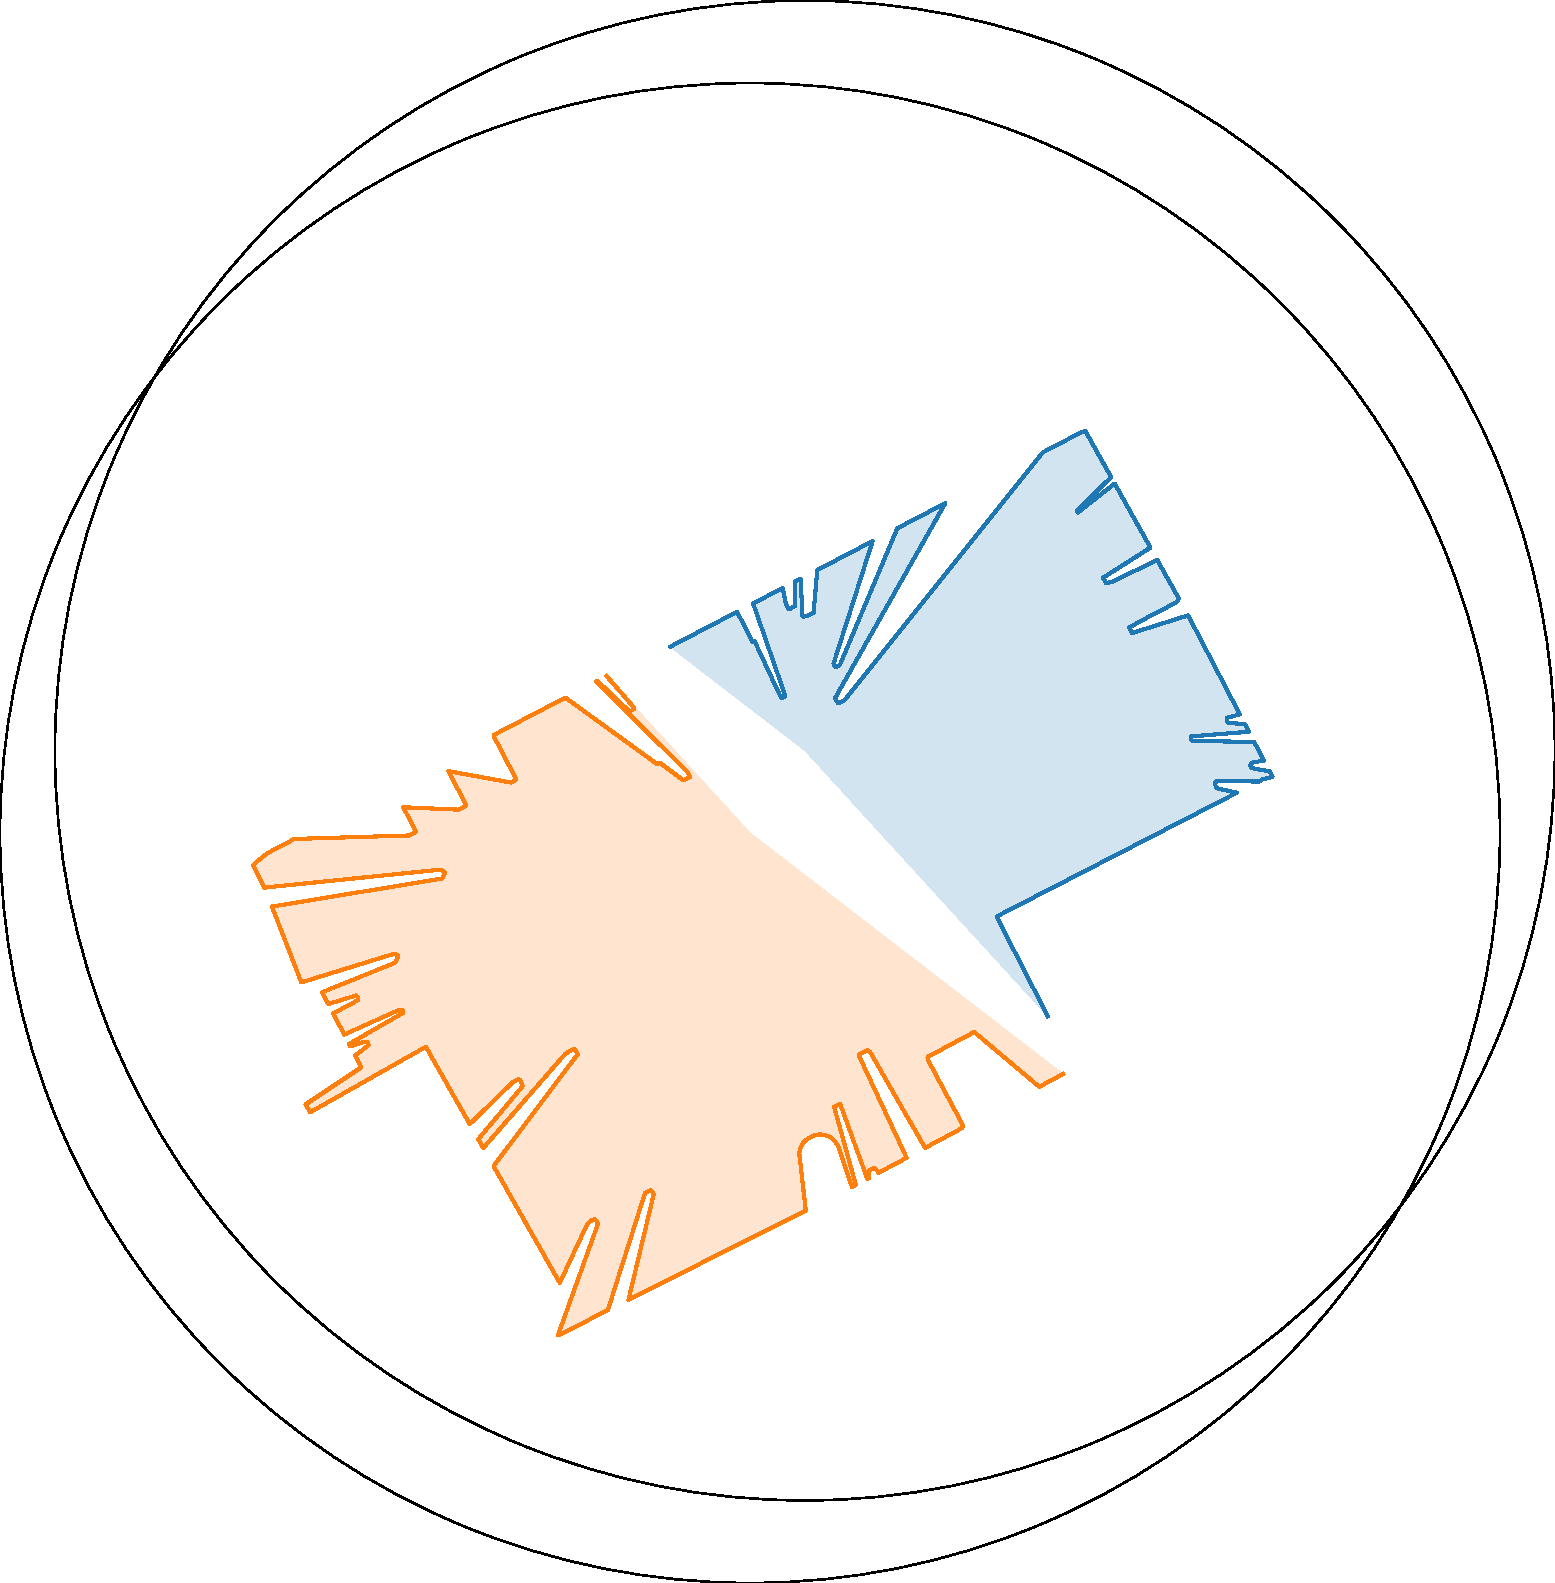
\includegraphics[width=0.31\linewidth]{figures/sim2real/lidar_sim_kitchen_table}
    \\\vspace{10pt}
    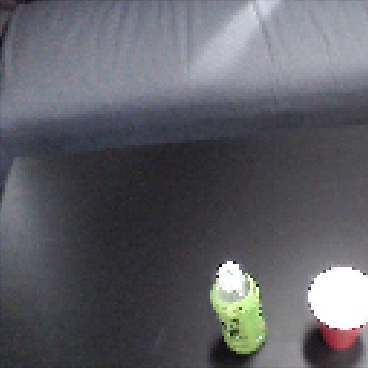
\includegraphics[width=0.31\linewidth]{figures/sim2real/rgb_real_coffee_table}
    \hfill
    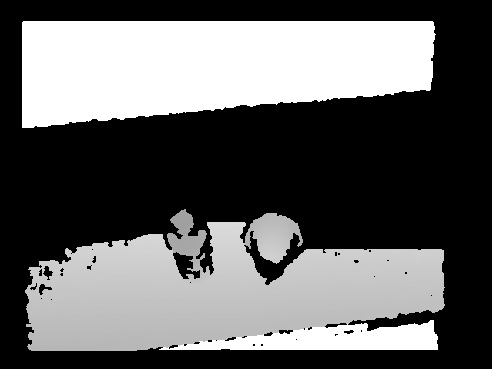
\includegraphics[width=0.31\linewidth]{figures/sim2real/depth_real_coffee_table}
    \hfill
    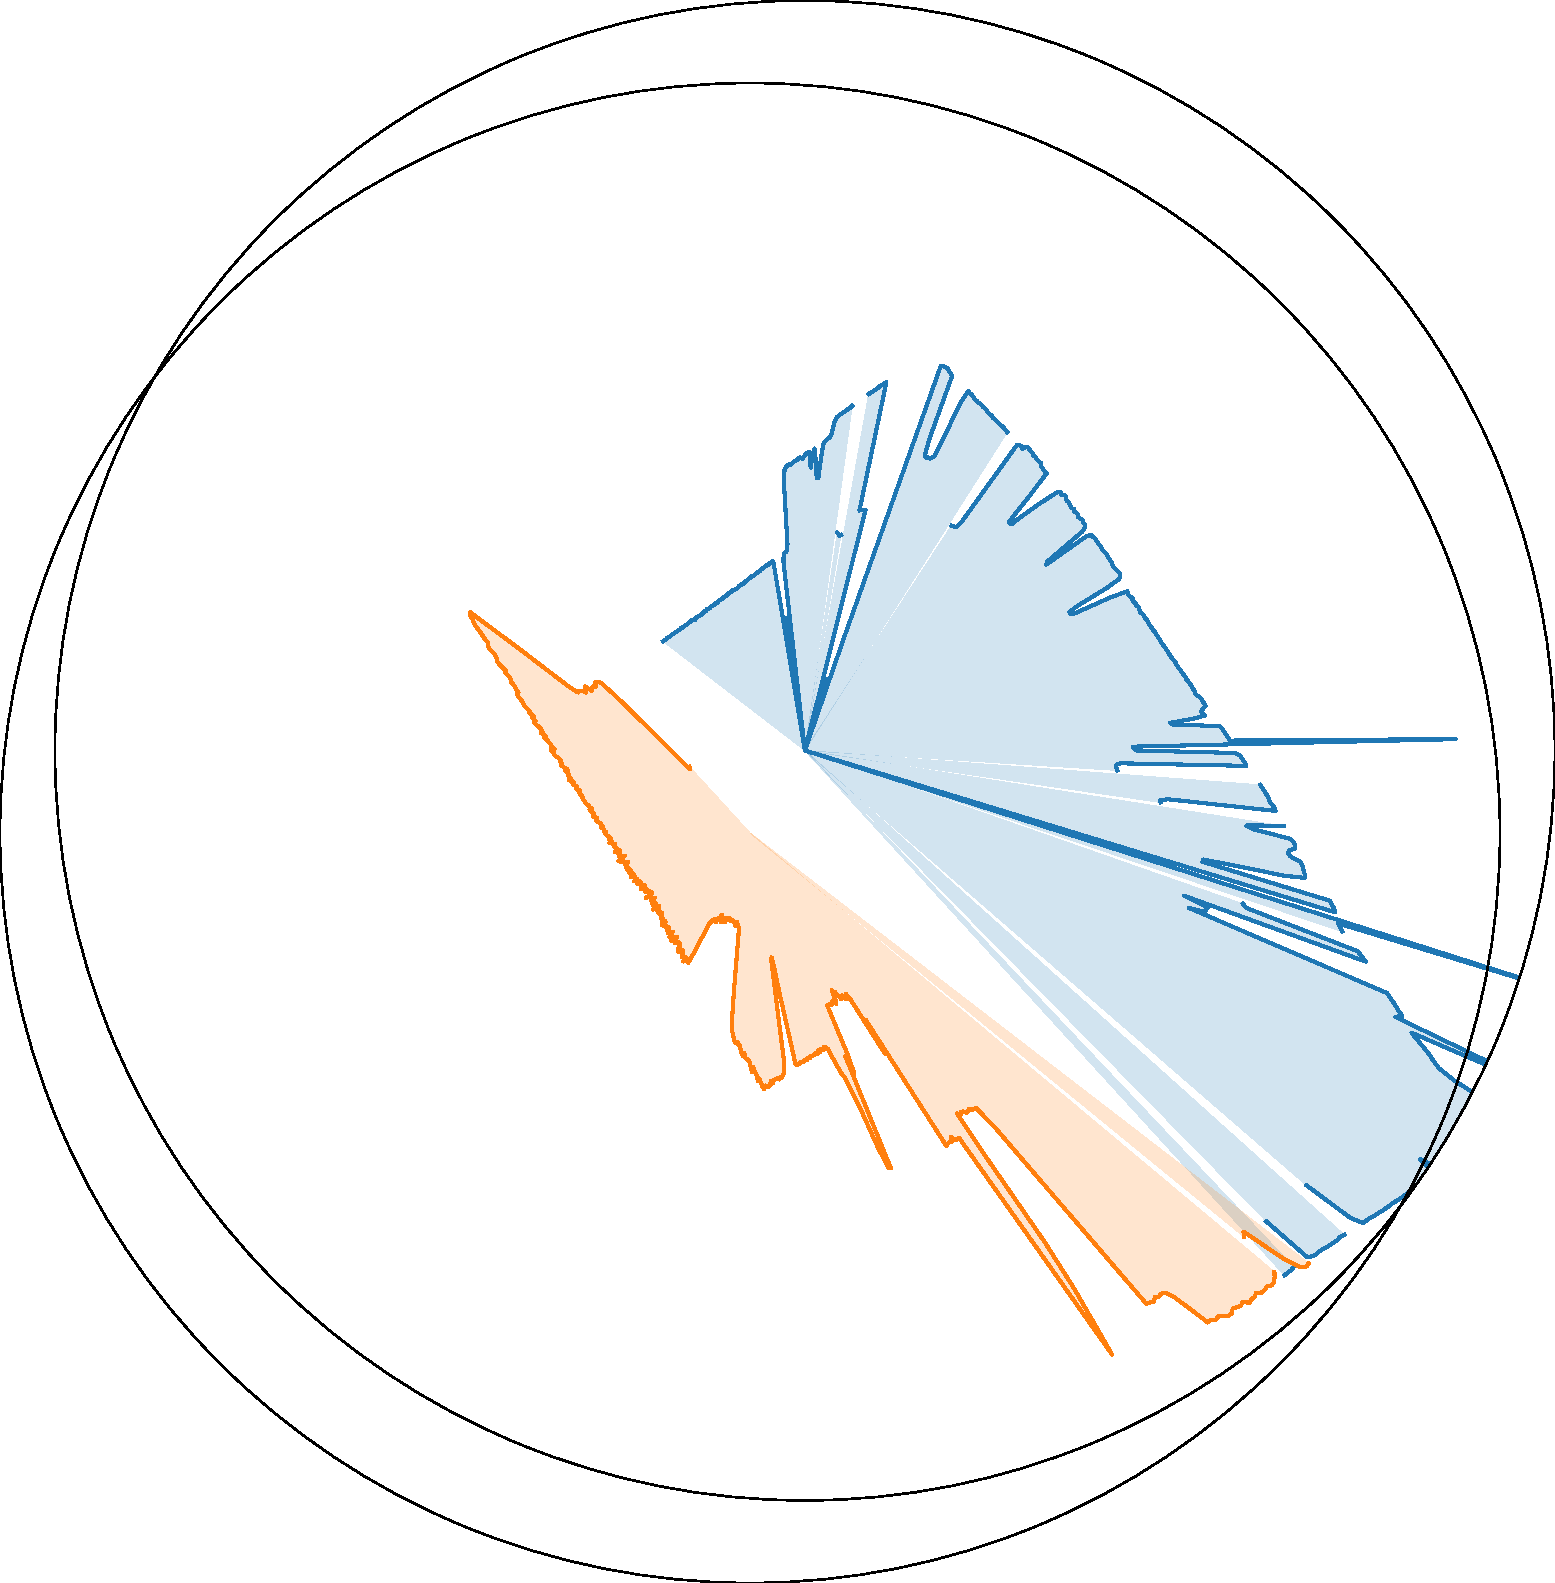
\includegraphics[width=0.31\linewidth]{figures/sim2real/lidar_real_coffee_table}
    \\\vspace{3pt}
    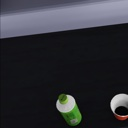
\includegraphics[width=0.31\linewidth]{figures/sim2real/rgb_sim_coffee_table.jpg}
    \hfill
    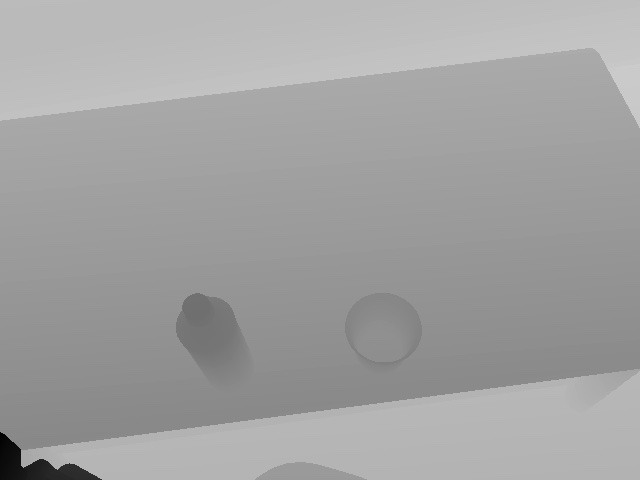
\includegraphics[width=0.31\linewidth]{figures/sim2real/depth_sim_coffee_table.jpg}
    \hfill
    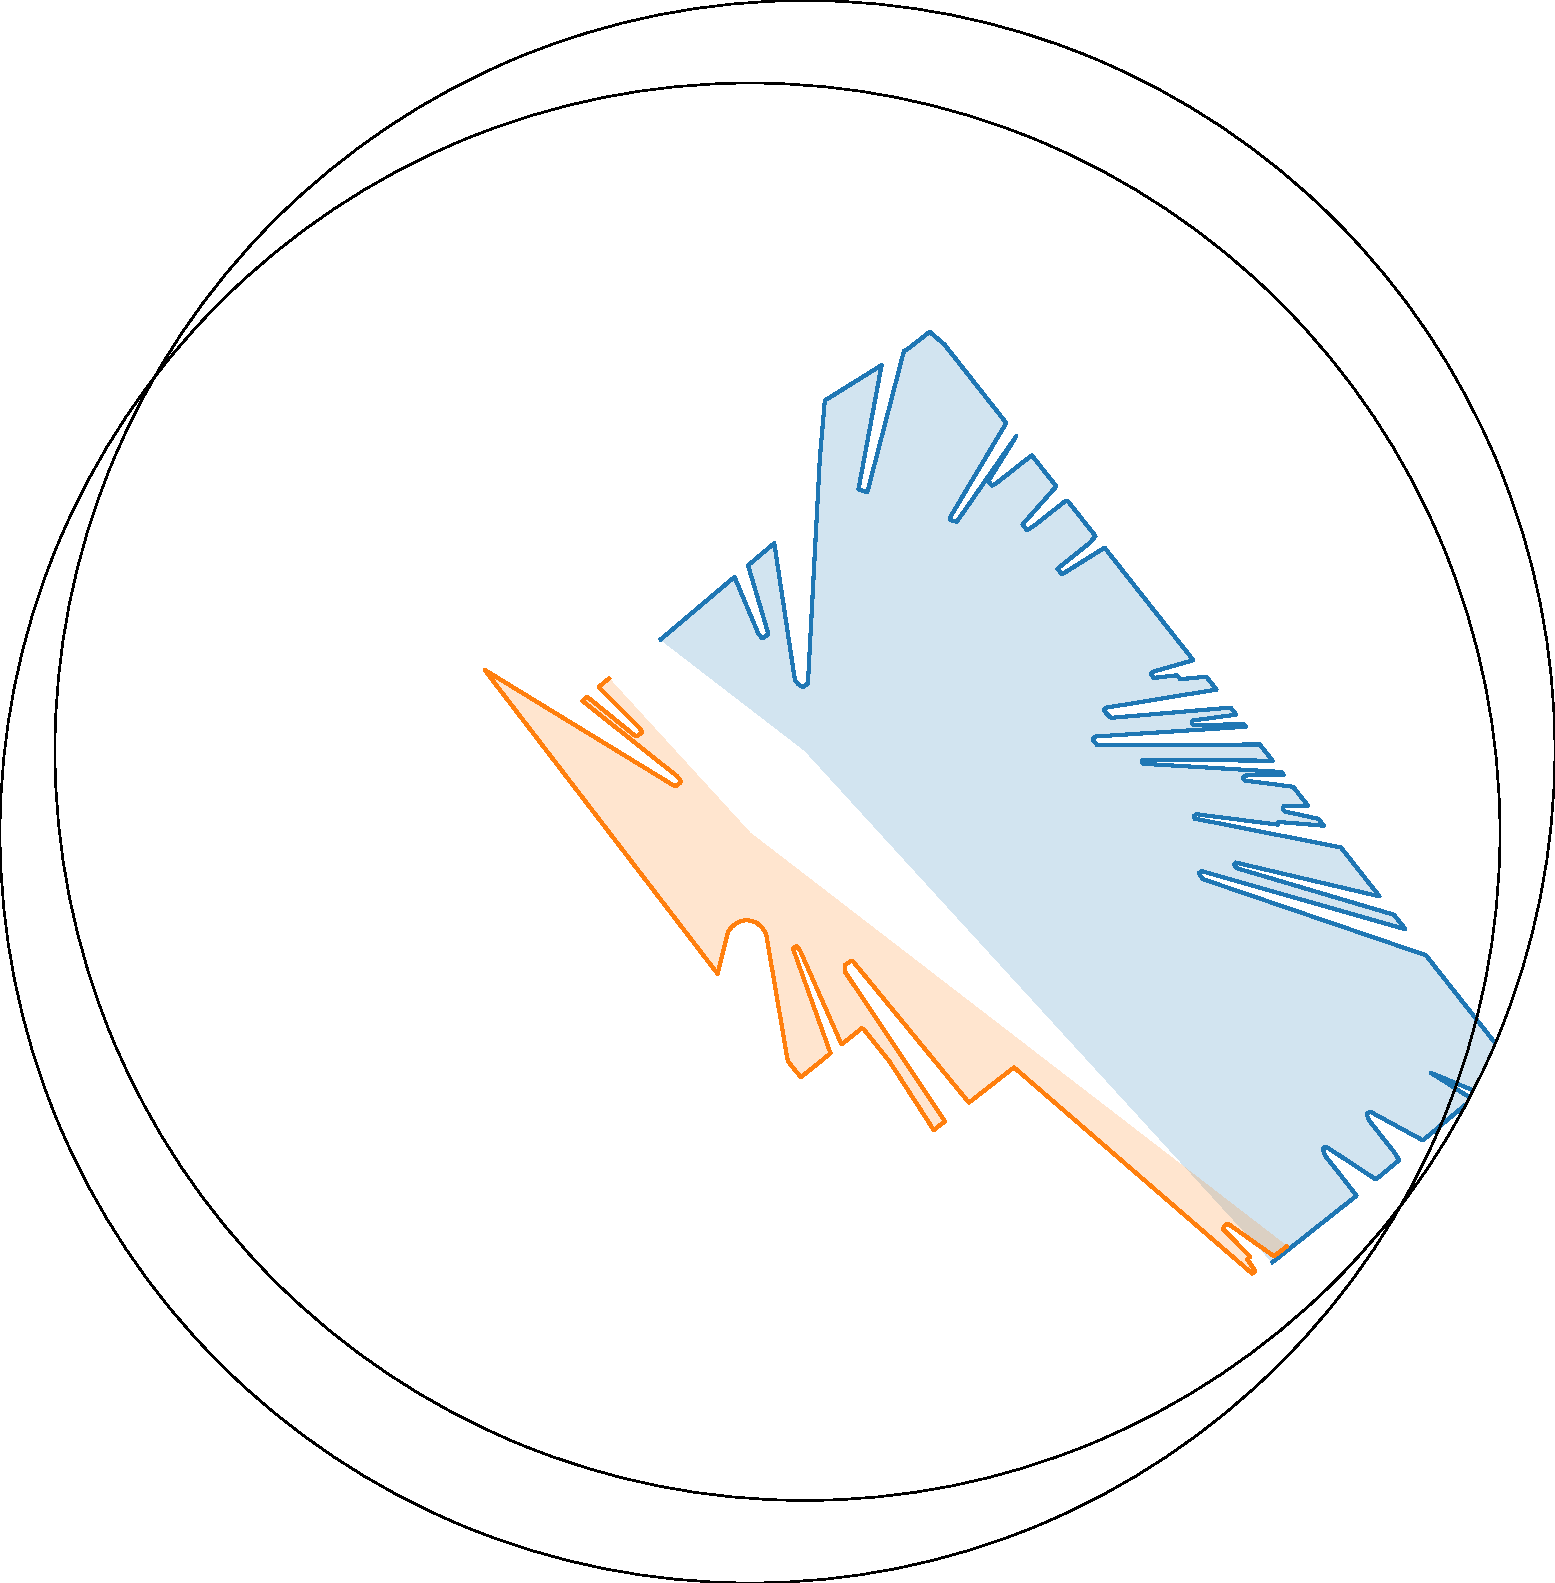
\includegraphics[width=0.31\linewidth]{figures/sim2real/lidar_sim_coffee_table}
    %    \caption{\textbf{Comparison between simulated and real sensor signals.} From left to right: RGB, Depth and Lidar signals in simulation (first and third rows) and from the real-world sensors (second and third rows) in two different locations of the \texttt{mockup\_apt} scene (location 1: first two rows, location 2: last two rows). Apart from some unmodeled sources of noise in the real-sensors, we observe a high realism in the signals generated in \simulator.}
    \caption{\revision{\textbf{Comparison between real and simulated sensor signals.} RGB, Depth and LiDAR signals from the real-world sensors (first and third rows) and from the simulated sensors (second and fourth rows) at two different locations of the \texttt{mockup\_apt} scene (location 1: first two rows, location 2: last two rows). We observed a smaller sensor sim-real gap for LiDAR than for RGB and Depth: RGB is heavily influenced by lighting conditions and camera settings while Depth has difficulty in capturing reflective surfaces.}}
    \label{fig:simrealsensors}
\end{figure}

\section{Ethical Statement}

\benchmark aims to drive embodied AI solutions that fulfill human need. A primary ethical consideration of \benchmark is therefore the method used to determine such need. To understand which activities would be useful for humans, we survey 1,461 respondents on Amazon Mechanical Turk and collected 50 responses for each activity, aiming for a clear consensus signal. Though this is a large group, the results are still biased by the fact that the researchers, annotators, and data providers only represent a small population relative to potential users of such technology. We plan to address these biases by making \dataset open-source and invite a wider community to contribute to its knowledge base. 

Furthermore, compared to the U.S. population, the demographic representation in our survey skews white, male, non-disability status, mid-five figure incomes, and 30-40 age range with more representation on the higher side than the lower side of that range\textemdash closer to the demographics of Mechanical Turk workers. This also biases the survey population toward certain responses, creating potential ethical limitations. 

Specifically this bias may affect the survey's representation of people who would be affected most by autonomous agents~\cite{mckinsey2019automation}. We therefore asked several explicit questions such as ``Do you do household work for a living?'', ``If you do household work for a living, would you benefit from assistance?'',  ``Do you pay for someone else to do household work for you?''. Future work involves using these questions to direct benchmark development. 




%\bibliographystyleA{unsrt}
%\bibliographyA{ref}

\newpage
\definecolor{main-color}{rgb}{0,0,0}
\definecolor{back-color}{rgb}{0.942, 0.942, 0.93}
\definecolor{string-color}{rgb}{0.3333, 0.5254, 0.345}
\definecolor{key-color}{rgb}{0.847, 0.1059, 0.3765}
\definecolor{pred-color}{rgb}{0.1176, 0.5333, 0.898}
\definecolor{term-color}{rgb}{0., 0.31, 0.251}

\lstdefinestyle{mystyle}
{
    language = C,
    basicstyle = {\tiny \ttfamily \color{main-color}},
    backgroundcolor = {\color{back-color}},
    stringstyle = {\color{string-color}},
    keywordstyle = [2]{\color{pred-color}},
    keywordstyle = [3]{\color{key-color}},
    keywordstyle = {\color{term-color}},
    otherkeywords = {?},
    morekeywords = [2]{ontop, inside, inroom},
    morekeywords = [3]{define, problem, domain, objects, init, goal, and, for_n_pairs, forall, :, exists, and},
}

\noindent\begin{minipage}[t]{0.85\textwidth}
\begin{lstlisting}[style = mystyle,
  caption={{\texttt{BakingSugarCookies}}}, label={lst:bddl3}]
(define (problem baking_sugar_cookies-0)
    (:domain omnigibson)

    (:objects
        flour.n.01_1 - flour.n.01
        granulated_sugar.n.01_1 - granulated_sugar.n.01
        raw_egg.n.01_1 - raw_egg.n.01
        vanilla.n.02_1 - vanilla.n.02
        melted__butter.n.01_1 - melted__butter.n.01
        sodium_carbonate.n.01_1 - sodium_carbonate.n.01
        baking_powder.n.01_1 - baking_powder.n.01
        electric_mixer.n.01_1 - electric_mixer.n.01
        mixing_bowl.n.01_1 - mixing_bowl.n.01
        sugar_cookie.n.01_1 sugar_cookie.n.01_2 sugar_cookie.n.01_3
        sugar_cookie.n.01_4 sugar_cookie.n.01_5 sugar_cookie.n.01_6 - sugar_cookie.n.01
        oven.n.01_1 - oven.n.01
        cookie_sheet.n.01_1 - cookie_sheet.n.01
        flour__sack.n.01_1 - flour__sack.n.01
        sugar__sack.n.01_1 - sugar__sack.n.01
        sodium_carbonate__jar.n.01_1 - sodium_carbonate__jar.n.01
        baking_powder__jar.n.01_1 - baking_powder__jar.n.01
        mason_jar.n.01_1 - mason_jar.n.01
        countertop.n.01_1 countertop.n.01_2 - countertop.n.01
        vanilla__bottle.n.01_1 - vanilla__bottle.n.01
        salt.n.02_1 - salt.n.02
        salt__shaker.n.01_1 - salt__shaker.n.01
        bowl.n.01_1 - bowl.n.01
        electric_refrigerator.n.01_1 - electric_refrigerator.n.01
        tablespoon.n.02_1 - tablespoon.n.02
        floor.n.01_1 - floor.n.01
        agent.n.01_1 - agent.n.01
    )
    
    (:init 
        (filled flour__sack.n.01_1 flour.n.01_1)
        (ontop flour__sack.n.01_1 countertop.n.01_1)
        (insource salt__shaker.n.01_1 salt.n.02_1)
        (ontop salt__shaker.n.01_1 countertop.n.01_1)
        (ontop tablespoon.n.02_1 countertop.n.01_1)
        (filled sugar__sack.n.01_1 granulated_sugar.n.01_1)
        (ontop sugar__sack.n.01_1 countertop.n.01_1)
        (inside raw_egg.n.01_1 bowl.n.01_1)
        (insource vanilla__bottle.n.01_1 vanilla.n.02_1)
        (ontop vanilla__bottle.n.01_1 countertop.n.01_1)
        (filled mason_jar.n.01_1 melted__butter.n.01_1)
        (ontop mason_jar.n.01_1 countertop.n.01_1)
        (filled sodium_carbonate__jar.n.01_1 sodium_carbonate.n.01_1)
        (ontop sodium_carbonate__jar.n.01_1 countertop.n.01_2)
        (filled baking_powder__jar.n.01_1 baking_powder.n.01_1)
        (ontop baking_powder__jar.n.01_1 countertop.n.01_2)
        (ontop electric_mixer.n.01_1 countertop.n.01_2)
        (attached mixing_bowl.n.01_1 electric_mixer.n.01_1)
        (inroom oven.n.01_1 kitchen)
        (inroom countertop.n.01_1 kitchen)
        (inroom countertop.n.01_2 kitchen)
        (inside bowl.n.01_1 electric_refrigerator.n.01_1)
        (inroom electric_refrigerator.n.01_1 kitchen)
        (ontop cookie_sheet.n.01_1 countertop.n.01_2)
        (inroom floor.n.01_1 kitchen) 
        (ontop agent.n.01_1 floor.n.01_1)
        (future sugar_cookie.n.01_4) 
        (future sugar_cookie.n.01_1) 
        (future sugar_cookie.n.01_2) 
        (future sugar_cookie.n.01_6) 
        (future sugar_cookie.n.01_3) 
        (future sugar_cookie.n.01_5) 
    )
    
    (:goal 
        (and 
            (real ?sugar_cookie.n.01_1) 
            (real ?sugar_cookie.n.01_2) 
            (real ?sugar_cookie.n.01_3) 
            (real ?sugar_cookie.n.01_4) 
            (real ?sugar_cookie.n.01_5) 
            (real ?sugar_cookie.n.01_6) 
            (forall 
                (?sugar_cookie.n.01 - sugar_cookie.n.01) 
                (and 
                    (cooked ?sugar_cookie.n.01) 
                    (ontop ?sugar_cookie.n.01 ?cookie_sheet.n.01_1)
                )
            )
        )
    )
)
\end{lstlisting}
\end{minipage}


\begin{minipage}[t]{.45\textwidth}
\begin{lstlisting}[style = mystyle, caption={{\texttt{CleanYourLaundryRoom}}}, label={lst:bddl4}]
(define 
  (problem clean_your_laundry_room_1)
  (:domain omnigibson)
    
  (:objects
    rag.n.01_1 - rag.n.01
    dryer.n.01_1 - dryer.n.01
    water.n.06_1 - water.n.06
    vinegar.n.01_1 - vinegar.n.01
    washer.n.03_1 - washer.n.03
    dust.n.01_1 - dust.n.01
    mold.n.05_1 - mold.n.05
    floor.n.01_1 - floor.n.01
    agent.n.01_1 - agent.n.01
  )
    
  (:init 
    (ontop rag.n.01_1 dryer.n.01_1) 
    (not 
      (covered water.n.06_1 rag.n.01_1)
    ) 
    (empty vinegar.n.01_1 washer.n.03_1) 
    (covered dust.n.01_1 dryer.n.01_1) 
    (covered mold.n.05_1 washer.n.03_1) 
    (onfloor agent.n.01_1 floor.n.01_1) 
    (filled water.n.06_1 bottle.n.01_1) 
    (onfloor bottle.n.01_1 floor.n.01_1)
    (inroom washer.n.03_1 laundry_room)
    (inroom floor.n.01_1 laundry_room)
  )
    
  (:goal 
    (and 
      (filled ?vinegar.n.01_1 ?washer.n.03_1) 
      (not 
        (covered ?dust.n.01_1 ?dryer.n.01_1)
      ) 
      (not 
        (covered ?mold.n.05_1 ?washer.n.03_1)
      )
    )
  )
)
\end{lstlisting}
\end{minipage}\hfill
\begin{minipage}[t]{.52\textwidth}
\begin{lstlisting}[style = mystyle, caption={{\texttt{CleanTheBottomOfAnIron}}}, label={lst:bddl5}]
(define (problem clean_the_bottom_of_an_iron-0)
    (:domain omnigibson)

    (:objects
        tarnish.n.02_1 - tarnish.n.02
        iron.n.04_1 - iron.n.04
        ironing_board.n.01_1 - ironing_board.n.01
        emery_paper.n.01_1 - emery_paper.n.01
        countertop.n.01_1 - countertop.n.01
        newspaper.n.03_1 - newspaper.n.03
        floor.n.01_1 - floor.n.01
        agent.n.01_1 - agent.n.01
    )
    
    (:init 
        (covered iron.n.04_1 tarnish.n.02_1)
        (toggled_on iron.n.04_1) 
        (ontop iron.n.04_1 ironing_board.n.01_1) 
        (ontop ironing_board.n.01_1 floor.n.01_1) 
        (ontop emery_paper.n.01_1 countertop.n.01_1)
        (ontop newspaper.n.03_1 ironing_board.n.01_1) 
        (inroom countertop.n.01_1 utility_room) 
        (inroom floor.n.01_1 utility_room) 
        (ontop agent.n.01_1 floor.n.01_1)
    )
    
    (:goal 
        (and
            (not 
                (covered ?iron.n.04_1 ?tarnish.n.02_1)
            )
        )
    )
)
\end{lstlisting}
\end{minipage}


\begin{minipage}[t]{.45\textwidth}
\begin{lstlisting}[style = mystyle, caption={{\texttt{PackingLunch}}}, label={lst:bddl1}]
(define 
  (problem packing_lunches_1)
  (:domain igibson)
    
  (:objects
    shelf.n.01_1 - shelf.n.01
    water.n.06_1 - water.n.06
    countertop.n.01_1 - countertop.n.01
    apple.n.01_1 - apple.n.01
    electric_refrigerator.n.01_1 - 
        electric_refrigerator.n.01
    hamburger.n.01_1 - hamburger.n.01
    basket.n.01_1 - basket.n.01
  )
    
  (:init 
    (ontop water.n.06_1 countertop.n.01_1)
    (inside apple.n.01_1 
        electric_refrigerator.n.01_1)
    (inside hamburger.n.01_1 
        electric_refrigerator.n.01_1)
    (ontop basket.n.01_1 countertop.n.01_1) 
    (inroom countertop.n.01_1 kitchen) 
    (inroom electric_refrigerator.n.01_1 
        kitchen) 
    (inroom shelf.n.01_1 kitchen)
  )
    
  (:goal 
    (and 
      (for_n_pairs
        (1)
        (?hamburger.n.01 - hamburger.n.01)
        (?basket.n.01 - basket.n.01)
        (inside ?hamburger.n.01 ?basket.n.01)
      )
      (for_n_pairs 
        (1) 
        (?basket.n.01 - basket.n.01) 
        (?water.n.06 - water.n.06) 
        (inside ?water.n.06 ?basket.n.01)
      ) 
      (for_n_pairs 
        (1) 
        (?basket.n.01 - basket.n.01) 
        (?apple.n.01 - apple.n.01) 
        (inside ?apple.n.01 ?basket.n.01)
      ) 
      (forall 
        (?basket.n.01 - basket.n.01) 
        (ontop ?basket.n.01 ?countertop.n.01_1) 
      )
    )
  )
)
\end{lstlisting}
\end{minipage}\hfill
\begin{minipage}[t]{.47\textwidth}
\begin{lstlisting}[style=mystyle, caption={{\texttt{ServingHorsDoeuvres}}}, label={lst:bddl2}]
(define 
  (problem serving_hors_d_oeuvres_1)
  (:domain igibson)

  (:objects
    tray.n.01_1 tray.n.01_2 - tray.n.01
    countertop.n.01_1 - countertop.n.01
    oven.n.01_1 - oven.n.01
    sausage.n.01_1 sausage.n.01_2 - sausage.n.01
    cherry.n.03_1 cherry.n.03_2 - cherry.n.03
    electric_refrigerator.n.01_1 - 
        electric_refrigerator.n.01
  )
    
  (:init 
    (ontop tray.n.01_1 countertop.n.01_1)
    (ontop tray.n.01_2 countertop.n.01_1)
    (inside sausage.n.01_1 oven.n.01_1)
    (inside sausage.n.01_2 oven.n.01_1)
    (inside cherry.n.03_1 
        electric_refrigerator.n.01_1)
    (inside cherry.n.03_2 
        electric_refrigerator.n.01_1)
    (inroom oven.n.01_1 kitchen)
    (inroom electric_refrigerator.n.01_1 
        kitchen)
    (inroom countertop.n.01_1 kitchen)
  )

  (:goal
    (and
      (exists
        (?tray.n.01 - tray.n.01)
        (and
          (forall
            (?sausage.n.01 - sausage.n.01)
            (ontop ?sausage.n.01 ?tray.n.01)
          )
          (forall
            (?cherry.n.03 - cherry.n.03)
            (not
              (ontop ?cherry.n.03 ?tray.n.01)
            )
          )
        )
      )
      (exists
        (?tray.n.01 - tray.n.01)
        (and
          (forall
            (?cherry.n.03 - cherry.n.03)
            (ontop ?cherry.n.03 ?tray.n.01)
          )
          (forall
            (?sausage.n.01 - sausage.n.01)
            (not
              (ontop ?sausage.n.01 ?tray.n.01)
            )
          )
        )
      )
    )
  )
)
\end{lstlisting}
\end{minipage}

\end{document}
